\documentclass[]{book}
\usepackage{lmodern}
\usepackage{amssymb,amsmath}
\usepackage{ifxetex,ifluatex}
\usepackage{fixltx2e} % provides \textsubscript
\ifnum 0\ifxetex 1\fi\ifluatex 1\fi=0 % if pdftex
  \usepackage[T1]{fontenc}
  \usepackage[utf8]{inputenc}
\else % if luatex or xelatex
  \ifxetex
    \usepackage{mathspec}
  \else
    \usepackage{fontspec}
  \fi
  \defaultfontfeatures{Ligatures=TeX,Scale=MatchLowercase}
\fi
% use upquote if available, for straight quotes in verbatim environments
\IfFileExists{upquote.sty}{\usepackage{upquote}}{}
% use microtype if available
\IfFileExists{microtype.sty}{%
\usepackage{microtype}
\UseMicrotypeSet[protrusion]{basicmath} % disable protrusion for tt fonts
}{}
\usepackage[margin=1in]{geometry}
\usepackage{hyperref}
\PassOptionsToPackage{usenames,dvipsnames}{color} % color is loaded by hyperref
\hypersetup{unicode=true,
            pdftitle={The Good Loser},
            pdfauthor={Peter Esaiasson, Sveinung Arnesen, and Hannah Werner},
            colorlinks=true,
            linkcolor=Maroon,
            citecolor=Blue,
            urlcolor=Blue,
            breaklinks=true}
\urlstyle{same}  % don't use monospace font for urls
\usepackage{natbib}
\bibliographystyle{apalike}
\usepackage{color}
\usepackage{fancyvrb}
\newcommand{\VerbBar}{|}
\newcommand{\VERB}{\Verb[commandchars=\\\{\}]}
\DefineVerbatimEnvironment{Highlighting}{Verbatim}{commandchars=\\\{\}}
% Add ',fontsize=\small' for more characters per line
\usepackage{framed}
\definecolor{shadecolor}{RGB}{248,248,248}
\newenvironment{Shaded}{\begin{snugshade}}{\end{snugshade}}
\newcommand{\KeywordTok}[1]{\textcolor[rgb]{0.13,0.29,0.53}{\textbf{#1}}}
\newcommand{\DataTypeTok}[1]{\textcolor[rgb]{0.13,0.29,0.53}{#1}}
\newcommand{\DecValTok}[1]{\textcolor[rgb]{0.00,0.00,0.81}{#1}}
\newcommand{\BaseNTok}[1]{\textcolor[rgb]{0.00,0.00,0.81}{#1}}
\newcommand{\FloatTok}[1]{\textcolor[rgb]{0.00,0.00,0.81}{#1}}
\newcommand{\ConstantTok}[1]{\textcolor[rgb]{0.00,0.00,0.00}{#1}}
\newcommand{\CharTok}[1]{\textcolor[rgb]{0.31,0.60,0.02}{#1}}
\newcommand{\SpecialCharTok}[1]{\textcolor[rgb]{0.00,0.00,0.00}{#1}}
\newcommand{\StringTok}[1]{\textcolor[rgb]{0.31,0.60,0.02}{#1}}
\newcommand{\VerbatimStringTok}[1]{\textcolor[rgb]{0.31,0.60,0.02}{#1}}
\newcommand{\SpecialStringTok}[1]{\textcolor[rgb]{0.31,0.60,0.02}{#1}}
\newcommand{\ImportTok}[1]{#1}
\newcommand{\CommentTok}[1]{\textcolor[rgb]{0.56,0.35,0.01}{\textit{#1}}}
\newcommand{\DocumentationTok}[1]{\textcolor[rgb]{0.56,0.35,0.01}{\textbf{\textit{#1}}}}
\newcommand{\AnnotationTok}[1]{\textcolor[rgb]{0.56,0.35,0.01}{\textbf{\textit{#1}}}}
\newcommand{\CommentVarTok}[1]{\textcolor[rgb]{0.56,0.35,0.01}{\textbf{\textit{#1}}}}
\newcommand{\OtherTok}[1]{\textcolor[rgb]{0.56,0.35,0.01}{#1}}
\newcommand{\FunctionTok}[1]{\textcolor[rgb]{0.00,0.00,0.00}{#1}}
\newcommand{\VariableTok}[1]{\textcolor[rgb]{0.00,0.00,0.00}{#1}}
\newcommand{\ControlFlowTok}[1]{\textcolor[rgb]{0.13,0.29,0.53}{\textbf{#1}}}
\newcommand{\OperatorTok}[1]{\textcolor[rgb]{0.81,0.36,0.00}{\textbf{#1}}}
\newcommand{\BuiltInTok}[1]{#1}
\newcommand{\ExtensionTok}[1]{#1}
\newcommand{\PreprocessorTok}[1]{\textcolor[rgb]{0.56,0.35,0.01}{\textit{#1}}}
\newcommand{\AttributeTok}[1]{\textcolor[rgb]{0.77,0.63,0.00}{#1}}
\newcommand{\RegionMarkerTok}[1]{#1}
\newcommand{\InformationTok}[1]{\textcolor[rgb]{0.56,0.35,0.01}{\textbf{\textit{#1}}}}
\newcommand{\WarningTok}[1]{\textcolor[rgb]{0.56,0.35,0.01}{\textbf{\textit{#1}}}}
\newcommand{\AlertTok}[1]{\textcolor[rgb]{0.94,0.16,0.16}{#1}}
\newcommand{\ErrorTok}[1]{\textcolor[rgb]{0.64,0.00,0.00}{\textbf{#1}}}
\newcommand{\NormalTok}[1]{#1}
\usepackage{longtable,booktabs}
\usepackage{graphicx,grffile}
\makeatletter
\def\maxwidth{\ifdim\Gin@nat@width>\linewidth\linewidth\else\Gin@nat@width\fi}
\def\maxheight{\ifdim\Gin@nat@height>\textheight\textheight\else\Gin@nat@height\fi}
\makeatother
% Scale images if necessary, so that they will not overflow the page
% margins by default, and it is still possible to overwrite the defaults
% using explicit options in \includegraphics[width, height, ...]{}
\setkeys{Gin}{width=\maxwidth,height=\maxheight,keepaspectratio}
\IfFileExists{parskip.sty}{%
\usepackage{parskip}
}{% else
\setlength{\parindent}{0pt}
\setlength{\parskip}{6pt plus 2pt minus 1pt}
}
\setlength{\emergencystretch}{3em}  % prevent overfull lines
\providecommand{\tightlist}{%
  \setlength{\itemsep}{0pt}\setlength{\parskip}{0pt}}
\setcounter{secnumdepth}{5}
% Redefines (sub)paragraphs to behave more like sections
\ifx\paragraph\undefined\else
\let\oldparagraph\paragraph
\renewcommand{\paragraph}[1]{\oldparagraph{#1}\mbox{}}
\fi
\ifx\subparagraph\undefined\else
\let\oldsubparagraph\subparagraph
\renewcommand{\subparagraph}[1]{\oldsubparagraph{#1}\mbox{}}
\fi

%%% Use protect on footnotes to avoid problems with footnotes in titles
\let\rmarkdownfootnote\footnote%
\def\footnote{\protect\rmarkdownfootnote}

%%% Change title format to be more compact
\usepackage{titling}

% Create subtitle command for use in maketitle
\newcommand{\subtitle}[1]{
  \posttitle{
    \begin{center}\large#1\end{center}
    }
}

\setlength{\droptitle}{-2em}

  \title{The Good Loser}
    \pretitle{\vspace{\droptitle}\centering\huge}
  \posttitle{\par}
  \subtitle{Results from Three Survey Experiments}
  \author{Peter Esaiasson, Sveinung Arnesen, and Hannah Werner}
    \preauthor{\centering\large\emph}
  \postauthor{\par}
      \predate{\centering\large\emph}
  \postdate{\par}
    \date{2019-05-13}

\usepackage{booktabs}

\begin{document}
\maketitle

{
\hypersetup{linkcolor=black}
\setcounter{tocdepth}{1}
\tableofcontents
}
\chapter{Preface}\label{preface}

This is the analysis report for the \emph{Good Loser Project} by
\href{https://www.gu.se/omuniversitetet/personal/?userId=xesape}{Peter
Esaiasson},
\href{http://www.uva.nl/profiel/w/e/h.i.werner/h.i.werner.html}{Hannah
Werner}, and \href{http://frosty-bose-c7f82c.netlify.com/}{Sveinung
Arnesen}. The study comprises three survey embedded experiments; one
video vignette experiment in Norway, one text vignette experiment in
Sweden, and one conjoint experiment in Norway. The study has been
presented at the Barcelona-Gothenburg-Bergen workshop on Experiments in
Political Science in 2018, and will be presented at the 2019 Conference
of the Midwestern Political Science Association in Chicago, USA.

About Study I -- Swedish vignette: TBA

About Study II -- Norwegian video vignette: TBA

The conjoint experiment described in PART III was fielded in Norway
during the fall of 2018 through the 13th wave of
\href{https://www.uib.no/medborger}{Norwegian Citizen Panel (NCP)}. The
NCP is a research-purpose internet panel with over 6000 active
participants. It is based on a probability sample of the general
Norwegian population above the age of 18 drawn from the Norwegian
National Registry. The survey is based on a online questionnaire with
postal recruitment. Panel members complete a questionnaire three times a
year of 15 minutes each. The NCP is a core component of The Digital
Social Science Core Facilities (DIGSSCORE), and was established in 2013
as a collaboration between several departments at the Faculty of Social
Sciences at the University of Bergen and NORCE -- Norwegian Research
Centre. We refer to the
\href{Data/ncp-wave13-documentation.pdf}{documentation report} for
further details on technical aspects of the survey, panel recruitment,
response rates of the 13th wave, and representativeness. For details
about the data collected in this project and the NCP at large, we refer
to the \href{Data/ncp-wave13-codebook.pdf}{codebook for the Waves 1-13}.

\part{STUDY I: SWEDISH
VIGNETTE}\label{part-study-i-swedish-vignette}

INFO ABOUT THE SURVEY HERE

\chapter{Create Data Set}\label{create-data-set}

\section{Load packages or install them if not already
installed}\label{load-packages-or-install-them-if-not-already-installed}

\begin{Shaded}
\begin{Highlighting}[]
\ControlFlowTok{if}\NormalTok{(}\OperatorTok{!}\KeywordTok{require}\NormalTok{(}\StringTok{"haven"}\NormalTok{))\{}\KeywordTok{install.packages}\NormalTok{(}\StringTok{"haven"}\NormalTok{);  }\KeywordTok{library}\NormalTok{(haven)\}}
\ControlFlowTok{if}\NormalTok{(}\OperatorTok{!}\KeywordTok{require}\NormalTok{(}\StringTok{"tidyverse"}\NormalTok{))\{}\KeywordTok{install.packages}\NormalTok{(}\StringTok{"tidyverse"}\NormalTok{);  }\KeywordTok{library}\NormalTok{(tidyverse)\}}
\end{Highlighting}
\end{Shaded}

\section{Load raw Swedish Citizen Panel
data}\label{load-raw-swedish-citizen-panel-data}

Load data using the haven package. Select variables of interest, and
create new data set in .sav and .csv formats

\begin{Shaded}
\begin{Highlighting}[]
\NormalTok{scp_raw <-}\StringTok{ }\KeywordTok{read_sav}\NormalTok{(}\StringTok{"Data/Studie3_Esaiasson_20180611.sav"}\NormalTok{) }\OperatorTok\StringTok{ }
\StringTok{  }\KeywordTok{mutate}\NormalTok{(}\DataTypeTok{idnummer =} \KeywordTok{as.numeric}\NormalTok{(idnummer))}

\NormalTok{d  <-}\StringTok{ }\NormalTok{scp_raw }\OperatorTok\StringTok{  }\KeywordTok{select}\NormalTok{(}
\NormalTok{                       Q64, }\CommentTok{#age}
\NormalTok{                       Q63, }\CommentTok{#gender}
\NormalTok{                       S3_1_}\DecValTok{1}\NormalTok{,}
\NormalTok{                       S3_2_}\DecValTok{1}\NormalTok{,}
\NormalTok{                       S3_4_1_}\DecValTok{1}\NormalTok{,}
\NormalTok{                       S3_4_1_}\DecValTok{2}\NormalTok{,}
\NormalTok{                       S3_5_}\DecValTok{1}\NormalTok{,}
\NormalTok{                       S3_6_1_}\DecValTok{1}\NormalTok{,}
\NormalTok{                       S3_6_1_}\DecValTok{2}\NormalTok{,}
\NormalTok{                       S3_7_1_}\DecValTok{1}\NormalTok{,}
\NormalTok{                       S3_7_1_}\DecValTok{2}\NormalTok{,}
\NormalTok{                       S3_8_1_}\DecValTok{1}\NormalTok{,}
\NormalTok{                       S3_8_1_}\DecValTok{2}\NormalTok{,}
\NormalTok{                       Studie3sel}
\NormalTok{)}

\CommentTok{#Create data file, .csv format}
  \KeywordTok{write.csv}\NormalTok{(d, }\StringTok{"Data/Goodloser-exp1.csv"}\NormalTok{) }
  \CommentTok{#Create data file, .sav format}
  \KeywordTok{write_sav}\NormalTok{(d, }\StringTok{"Data/Goodloser-exp1.sav"}\NormalTok{, }\DataTypeTok{compress =} \OtherTok{FALSE}\NormalTok{) }
\end{Highlighting}
\end{Shaded}

\chapter{Codebook}\label{codebook}

\begin{quote}
This chapter displays the codebook for the data set of the first Good
Loser experiment, automatically generated using the R package
``codebook''.
\end{quote}

\begin{Shaded}
\begin{Highlighting}[]
\ControlFlowTok{if}\NormalTok{(}\OperatorTok{!}\KeywordTok{require}\NormalTok{(}\StringTok{"codebook"}\NormalTok{))\{}\KeywordTok{install.packages}\NormalTok{(}\StringTok{"codebook"}\NormalTok{);  }\KeywordTok{library}\NormalTok{(codebook)\}}
\ControlFlowTok{if}\NormalTok{(}\OperatorTok{!}\KeywordTok{require}\NormalTok{(}\StringTok{"haven"}\NormalTok{))\{}\KeywordTok{install.packages}\NormalTok{(}\StringTok{"haven"}\NormalTok{);  }\KeywordTok{library}\NormalTok{(haven)\}}
\end{Highlighting}
\end{Shaded}

\begin{Shaded}
\begin{Highlighting}[]
\NormalTok{d <-}\StringTok{ }\KeywordTok{read_sav}\NormalTok{(}\StringTok{"C:}\CharTok{\textbackslash{}\textbackslash{}}\StringTok{Users/Sveinung/OneDrive/NORCE 2018-/goodloser/Conjoint/Bookdown-goodloser/Data/Goodloser-exp1.sav"}\NormalTok{)}

\KeywordTok{detect_missings}\NormalTok{(d, }\DataTypeTok{ninety_nine_problems =} \OtherTok{TRUE}\NormalTok{, }\DataTypeTok{negative_values_are_missing =} \OtherTok{TRUE}\NormalTok{)}
\end{Highlighting}
\end{Shaded}

\begin{verbatim}
## # A tibble: 1,019 x 14
##      Q64 Q63   S3_1_1 S3_2_1 S3_4_1_1 S3_4_1_2 S3_5_1 S3_6_1_1 S3_6_1_2
##    <dbl> <dbl> <dbl+> <dbl+> <dbl+lb> <dbl+lb> <dbl+> <dbl+lb> <dbl+lb>
##  1    52 2     1      5      1        NA       4      1        NA      
##  2    30 2     2      3      4        NA       4      5        NA      
##  3    64 2     1      4      5        NA       2      2        NA      
##  4    43 2     2      2      4        NA       4      7        NA      
##  5    74 1     2      7      4        NA       4      4        NA      
##  6    51 2     1      4      1        NA       1      4        NA      
##  7    58 1     2      7      7        NA       7      6        NA      
##  8    55 1     2      4      4        NA       4      6        NA      
##  9    68 2     2      3      3        NA       3      3        NA      
## 10    32 1     2      5      6        NA       6      5        NA      
## # ... with 1,009 more rows, and 5 more variables: S3_7_1_1 <dbl+lbl>,
## #   S3_7_1_2 <dbl+lbl>, S3_8_1_1 <dbl+lbl>, S3_8_1_2 <dbl+lbl>,
## #   Studie3sel <dbl+lbl>
\end{verbatim}

\begin{Shaded}
\begin{Highlighting}[]
\KeywordTok{codebook}\NormalTok{(d)}
\end{Highlighting}
\end{Shaded}

\begin{verbatim}
## Warning in codebook(d): The variables session, created, ended have to
## be defined for automatic survey repetition detection to work. Set to no
## repetition by default.
\end{verbatim}

\begin{Shaded}
\begin{Highlighting}[]
\NormalTok{knitr}\OperatorTok{::}\KeywordTok{asis_output}\NormalTok{(survey_overview)}
\end{Highlighting}
\end{Shaded}

\section{Items}\label{items}

\begin{Shaded}
\begin{Highlighting}[]
\NormalTok{knitr}\OperatorTok{::}\KeywordTok{asis_output}\NormalTok{(}\KeywordTok{paste0}\NormalTok{(scales_items, }\DataTypeTok{sep =} \StringTok{"}\CharTok{\textbackslash{}n\textbackslash{}n\textbackslash{}n}\StringTok{"}\NormalTok{, }\DataTypeTok{collapse =} \StringTok{"}\CharTok{\textbackslash{}n\textbackslash{}n\textbackslash{}n}\StringTok{"}\NormalTok{))}
\end{Highlighting}
\end{Shaded}

\subsection{Q64}\label{Q64}

Ålder

\subsubsection{Distribution}\label{Q64_distribution}

\begin{Shaded}
\begin{Highlighting}[]
\NormalTok{show_missings <-}\StringTok{ }\OtherTok{FALSE}
\ControlFlowTok{if}\NormalTok{ (}\KeywordTok{has_label}\NormalTok{(item)) \{}
\NormalTok{  missings <-}\StringTok{ }\NormalTok{item[}\KeywordTok{is.na}\NormalTok{(haven}\OperatorTok{::}\KeywordTok{zap_missing}\NormalTok{(item))]}
  \KeywordTok{attributes}\NormalTok{(missings) <-}\StringTok{ }\KeywordTok{attributes}\NormalTok{(item)}
  \ControlFlowTok{if}\NormalTok{ (}\OperatorTok{!}\KeywordTok{is.null}\NormalTok{(}\KeywordTok{attributes}\NormalTok{(item)}\OperatorTok{$}\NormalTok{labels)) \{}
    \KeywordTok{attributes}\NormalTok{(missings)}\OperatorTok{$}\NormalTok{labels <-}\StringTok{ }\KeywordTok{attributes}\NormalTok{(missings)}\OperatorTok{$}\NormalTok{labels[}\KeywordTok{is.na}\NormalTok{(}\KeywordTok{attributes}\NormalTok{(missings)}\OperatorTok{$}\NormalTok{labels)]}
    \KeywordTok{attributes}\NormalTok{(item)}\OperatorTok{$}\NormalTok{labels <-}\StringTok{ }\KeywordTok{attributes}\NormalTok{(item)}\OperatorTok{$}\NormalTok{labels[}\OperatorTok{!}\KeywordTok{is.na}\NormalTok{(}\KeywordTok{attributes}\NormalTok{(item)}\OperatorTok{$}\NormalTok{labels)]}
\NormalTok{  \}}
  \ControlFlowTok{if}\NormalTok{ (}\KeywordTok{is.numeric}\NormalTok{(item)) \{}
\NormalTok{    show_missings <-}\StringTok{ }\KeywordTok{length}\NormalTok{(}\KeywordTok{unique}\NormalTok{(haven}\OperatorTok{::}\KeywordTok{na_tag}\NormalTok{(missings))) }\OperatorTok{>}\StringTok{ }\DecValTok{1}
\NormalTok{    item <-}\StringTok{ }\NormalTok{haven}\OperatorTok{::}\KeywordTok{zap_missing}\NormalTok{(item)}
\NormalTok{  \}}
  \ControlFlowTok{if}\NormalTok{ (}\KeywordTok{length}\NormalTok{(item_attributes}\OperatorTok{$}\NormalTok{labels) }\OperatorTok{==}\StringTok{ }\DecValTok{0} \OperatorTok{&&}\StringTok{ }\KeywordTok{is.numeric}\NormalTok{(item)) \{}
\NormalTok{    item <-}\StringTok{ }\NormalTok{haven}\OperatorTok{::}\KeywordTok{zap_labels}\NormalTok{(item)}
\NormalTok{  \}}
\NormalTok{\}}
\NormalTok{item_nomiss <-}\StringTok{ }\NormalTok{item[}\OperatorTok{!}\KeywordTok{is.na}\NormalTok{(item)]}

\CommentTok{# unnest mc_multiple and so on}
\ControlFlowTok{if}\NormalTok{ (}
  \KeywordTok{is.character}\NormalTok{(item_nomiss) }\OperatorTok{&&}
\StringTok{  }\NormalTok{stringr}\OperatorTok{::}\KeywordTok{str_detect}\NormalTok{(item_nomiss, stringr}\OperatorTok{::}\KeywordTok{fixed}\NormalTok{(}\StringTok{", "}\NormalTok{)) }\OperatorTok{&&}
\StringTok{  }\NormalTok{(}\KeywordTok{exists}\NormalTok{(}\StringTok{"type"}\NormalTok{, item_info) }\OperatorTok{&&}\StringTok{ }
\StringTok{    }\NormalTok{stringr}\OperatorTok{::}\KeywordTok{str_detect}\NormalTok{(item_info}\OperatorTok{$}\NormalTok{type, }\DataTypeTok{pattern =}\NormalTok{ stringr}\OperatorTok{::}\KeywordTok{fixed}\NormalTok{(}\StringTok{"multiple"}\NormalTok{)))}
\NormalTok{  ) \{}
\NormalTok{  item_nomiss <-}\StringTok{ }\KeywordTok{unlist}\NormalTok{(stringr}\OperatorTok{::}\KeywordTok{str_split}\NormalTok{(item_nomiss, }\DataTypeTok{pattern =}\NormalTok{ stringr}\OperatorTok{::}\KeywordTok{fixed}\NormalTok{(}\StringTok{", "}\NormalTok{)))}
\NormalTok{\}}
\KeywordTok{attributes}\NormalTok{(item_nomiss) <-}\StringTok{ }\KeywordTok{attributes}\NormalTok{(item)}

\NormalTok{old_height <-}\StringTok{ }\NormalTok{knitr}\OperatorTok{::}\NormalTok{opts_chunk}\OperatorTok{$}\KeywordTok{get}\NormalTok{(}\StringTok{"fig.height"}\NormalTok{)}
\NormalTok{non_missing_choices <-}\StringTok{ }\NormalTok{item_attributes[[}\StringTok{"labels"}\NormalTok{]]}
\NormalTok{many_labels <-}\StringTok{ }\KeywordTok{length}\NormalTok{(non_missing_choices) }\OperatorTok{>}\StringTok{ }\DecValTok{7}
\NormalTok{go_vertical <-}\StringTok{ }\OperatorTok{!}\KeywordTok{is.numeric}\NormalTok{(item_nomiss) }\OperatorTok{||}\StringTok{ }\NormalTok{many_labels}
\ControlFlowTok{if}\NormalTok{ ( go_vertical ) \{}
  \CommentTok{# numeric items are plotted horizontally (because that's what usually expected)}
  \CommentTok{# categorical items are plotted vertically because we can use the screen real estate better this way}

    \ControlFlowTok{if}\NormalTok{ (}\KeywordTok{is.null}\NormalTok{(choices) }\OperatorTok{||}\StringTok{ }
\StringTok{        }\NormalTok{dplyr}\OperatorTok{::}\KeywordTok{n_distinct}\NormalTok{(item_nomiss) }\OperatorTok{>}\StringTok{ }\KeywordTok{length}\NormalTok{(non_missing_choices)) \{}
\NormalTok{        non_missing_choices <-}\StringTok{ }\KeywordTok{unique}\NormalTok{(item_nomiss)}
        \KeywordTok{names}\NormalTok{(non_missing_choices) <-}\StringTok{ }\NormalTok{non_missing_choices}
\NormalTok{    \}}
\NormalTok{  choice_multiplier <-}\StringTok{ }\NormalTok{old_height}\OperatorTok{/}\FloatTok{6.5}
\NormalTok{    new_height <-}\StringTok{ }\DecValTok{2} \OperatorTok{+}\StringTok{ }\NormalTok{choice_multiplier }\OperatorTok{*}\StringTok{ }\KeywordTok{length}\NormalTok{(non_missing_choices)}
\NormalTok{    new_height <-}\StringTok{ }\KeywordTok{ifelse}\NormalTok{(new_height }\OperatorTok{>}\StringTok{ }\DecValTok{20}\NormalTok{, }\DecValTok{20}\NormalTok{, new_height)}
\NormalTok{    new_height <-}\StringTok{ }\KeywordTok{ifelse}\NormalTok{(new_height }\OperatorTok{<}\StringTok{ }\DecValTok{1}\NormalTok{, }\DecValTok{1}\NormalTok{, new_height)}
\NormalTok{    knitr}\OperatorTok{::}\NormalTok{opts_chunk}\OperatorTok{$}\KeywordTok{set}\NormalTok{(}\DataTypeTok{fig.height =}\NormalTok{ new_height)}
\NormalTok{\}}

\NormalTok{wrap_at <-}\StringTok{ }\NormalTok{knitr}\OperatorTok{::}\NormalTok{opts_chunk}\OperatorTok{$}\KeywordTok{get}\NormalTok{(}\StringTok{"fig.width"}\NormalTok{) }\OperatorTok{*}\StringTok{ }\DecValTok{10}
\end{Highlighting}
\end{Shaded}

\begin{Shaded}
\begin{Highlighting}[]
\CommentTok{# todo: if there are free-text choices mingled in with the pre-defined ones, don't show}
\CommentTok{# todo: show rare items if they are pre-defined}
\CommentTok{# todo: bin rare responses into "other category"}
\ControlFlowTok{if}\NormalTok{ (}\OperatorTok{!}\KeywordTok{length}\NormalTok{(item_nomiss)) \{}
  \KeywordTok{cat}\NormalTok{(}\StringTok{"No non-missing values to show."}\NormalTok{)}
\NormalTok{\} }\ControlFlowTok{else} \ControlFlowTok{if}\NormalTok{ (}\KeywordTok{is.numeric}\NormalTok{(item_nomiss) }\OperatorTok{||}\StringTok{ }\NormalTok{dplyr}\OperatorTok{::}\KeywordTok{n_distinct}\NormalTok{(item_nomiss) }\OperatorTok{<}\StringTok{ }\DecValTok{20}\NormalTok{) \{}
  \KeywordTok{plot_labelled}\NormalTok{(item_nomiss, item_name, wrap_at, go_vertical)}
\NormalTok{\} }\ControlFlowTok{else}\NormalTok{ \{}
    \KeywordTok{cat}\NormalTok{(dplyr}\OperatorTok{::}\KeywordTok{n_distinct}\NormalTok{(item_nomiss), }\StringTok{" unique, categorical values, so not shown."}\NormalTok{)}
\NormalTok{\}}
\end{Highlighting}
\end{Shaded}

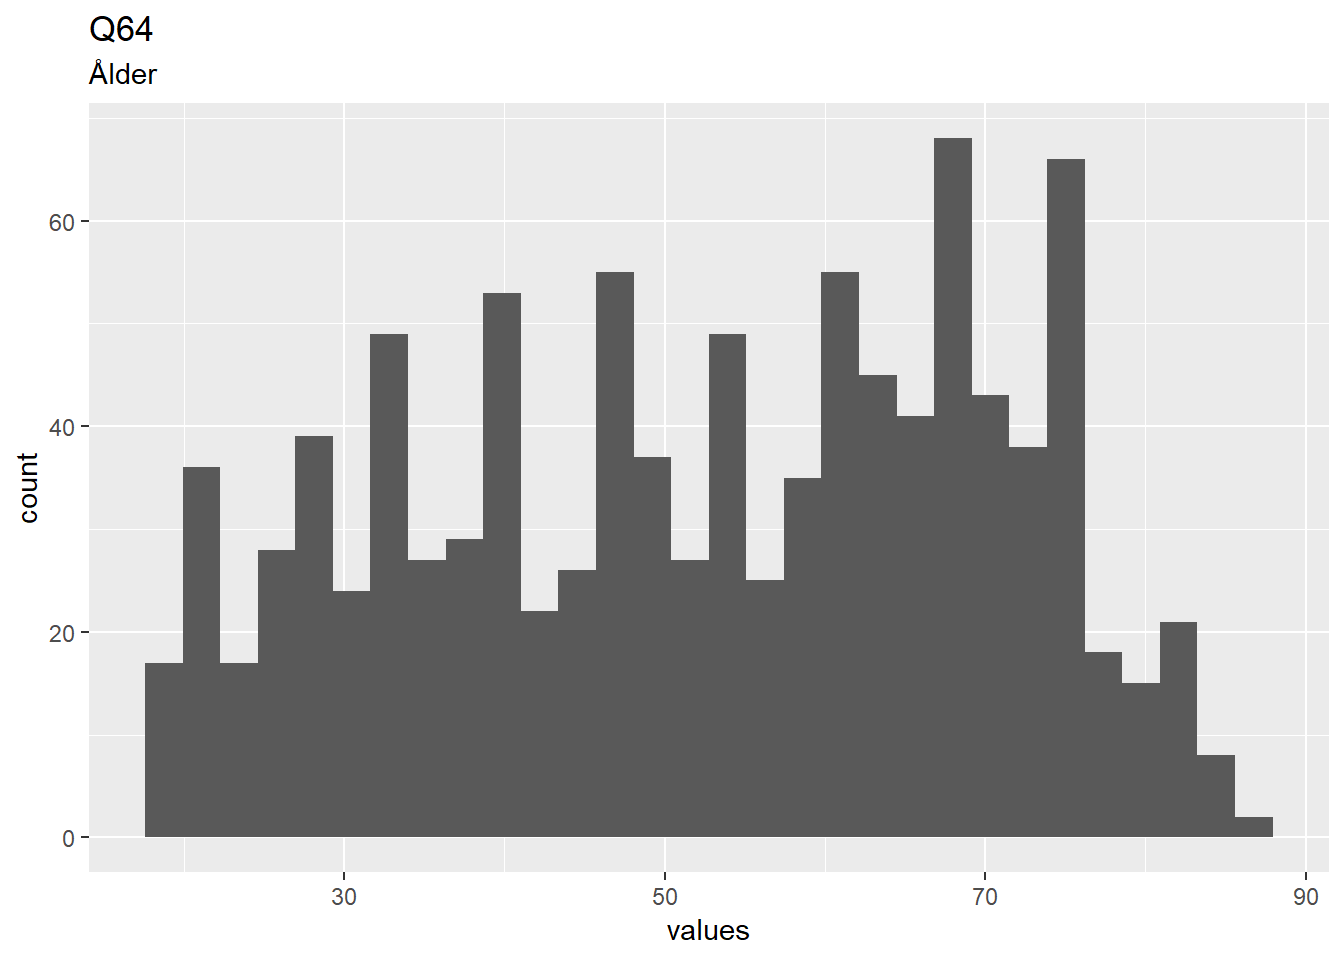
\includegraphics{Goodloser-appendix_files/figure-latex/Q64_distribution-1.pdf}

\begin{Shaded}
\begin{Highlighting}[]
\NormalTok{knitr}\OperatorTok{::}\NormalTok{opts_chunk}\OperatorTok{$}\KeywordTok{set}\NormalTok{(}\DataTypeTok{fig.height =}\NormalTok{ old_height)}
\end{Highlighting}
\end{Shaded}

4 missings.

\subsubsection{Summary statistics}\label{Q64_summary}

\begin{Shaded}
\begin{Highlighting}[]
\KeywordTok{attributes}\NormalTok{(item) <-}\StringTok{ }\NormalTok{item_attributes}
\NormalTok{df =}\StringTok{ }\KeywordTok{data.frame}\NormalTok{(item, }\DataTypeTok{stringsAsFactors =} \OtherTok{FALSE}\NormalTok{)}
\KeywordTok{names}\NormalTok{(df) =}\StringTok{ }\NormalTok{html_item_name}
\KeywordTok{escaped_table}\NormalTok{(}\KeywordTok{codebook_table}\NormalTok{(df))}
\end{Highlighting}
\end{Shaded}

name

label

data\_type

missing

complete

n

mean

sd

p0

p25

p50

p75

p100

hist

format.spss

display\_width

Q64

Ålder

numeric

4

1015

1019

52.46

17.74

18

38

54

68

86

▅▅▅▆▆▇▆▂

F8.0

10

\begin{Shaded}
\begin{Highlighting}[]
\ControlFlowTok{if}\NormalTok{ (show_missings) \{}
  \KeywordTok{plot_labelled}\NormalTok{(missings, item_name, wrap_at)}
\NormalTok{\}}
\end{Highlighting}
\end{Shaded}

\begin{Shaded}
\begin{Highlighting}[]
\ControlFlowTok{if}\NormalTok{ (}\OperatorTok{!}\KeywordTok{is.null}\NormalTok{(item_info)) \{}
  \CommentTok{# don't show choices again, if they're basically same thing as value labels}
  \ControlFlowTok{if}\NormalTok{ (}\OperatorTok{!}\KeywordTok{is.null}\NormalTok{(choices) }\OperatorTok{&&}\StringTok{ }\OperatorTok{!}\KeywordTok{is.null}\NormalTok{(item_info}\OperatorTok{$}\NormalTok{choices) }\OperatorTok{&&}\StringTok{ }
\StringTok{    }\KeywordTok{all}\NormalTok{(}\KeywordTok{names}\NormalTok{(}\KeywordTok{na.omit}\NormalTok{(choices)) }\OperatorTok{==}\StringTok{ }\NormalTok{item_info}\OperatorTok{$}\NormalTok{choices) }\OperatorTok{&&}
\StringTok{    }\KeywordTok{all}\NormalTok{(}\KeywordTok{na.omit}\NormalTok{(choices) }\OperatorTok{==}\StringTok{ }\KeywordTok{names}\NormalTok{(item_info}\OperatorTok{$}\NormalTok{choices))) \{}
\NormalTok{    item_info}\OperatorTok{$}\NormalTok{choices <-}\StringTok{ }\OtherTok{NULL}
\NormalTok{  \}}
\NormalTok{  item_info}\OperatorTok{$}\NormalTok{label_parsed <-}\StringTok{ }
\StringTok{    }\NormalTok{item_info}\OperatorTok{$}\NormalTok{choice_list <-}\StringTok{ }\NormalTok{item_info}\OperatorTok{$}\NormalTok{study_id <-}\StringTok{ }\NormalTok{item_info}\OperatorTok{$}\NormalTok{id <-}\StringTok{ }\OtherTok{NULL}
\NormalTok{  pander}\OperatorTok{::}\KeywordTok{pander}\NormalTok{(item_info)}
\NormalTok{\}}
\end{Highlighting}
\end{Shaded}

\begin{Shaded}
\begin{Highlighting}[]
\ControlFlowTok{if}\NormalTok{ (}\OperatorTok{!}\KeywordTok{is.null}\NormalTok{(choices) }\OperatorTok{&&}\StringTok{ }\KeywordTok{length}\NormalTok{(choices) }\OperatorTok{&&}\StringTok{ }\KeywordTok{length}\NormalTok{(choices) }\OperatorTok{<}\StringTok{ }\DecValTok{30}\NormalTok{) \{}
\NormalTok{    pander}\OperatorTok{::}\KeywordTok{pander}\NormalTok{(}\KeywordTok{as.list}\NormalTok{(choices))}
\NormalTok{\}}
\end{Highlighting}
\end{Shaded}

\subsection{Q63}\label{Q63}

Kön

\subsubsection{Distribution}\label{Q63_distribution}

\begin{Shaded}
\begin{Highlighting}[]
\NormalTok{show_missings <-}\StringTok{ }\OtherTok{FALSE}
\ControlFlowTok{if}\NormalTok{ (}\KeywordTok{has_label}\NormalTok{(item)) \{}
\NormalTok{  missings <-}\StringTok{ }\NormalTok{item[}\KeywordTok{is.na}\NormalTok{(haven}\OperatorTok{::}\KeywordTok{zap_missing}\NormalTok{(item))]}
  \KeywordTok{attributes}\NormalTok{(missings) <-}\StringTok{ }\KeywordTok{attributes}\NormalTok{(item)}
  \ControlFlowTok{if}\NormalTok{ (}\OperatorTok{!}\KeywordTok{is.null}\NormalTok{(}\KeywordTok{attributes}\NormalTok{(item)}\OperatorTok{$}\NormalTok{labels)) \{}
    \KeywordTok{attributes}\NormalTok{(missings)}\OperatorTok{$}\NormalTok{labels <-}\StringTok{ }\KeywordTok{attributes}\NormalTok{(missings)}\OperatorTok{$}\NormalTok{labels[}\KeywordTok{is.na}\NormalTok{(}\KeywordTok{attributes}\NormalTok{(missings)}\OperatorTok{$}\NormalTok{labels)]}
    \KeywordTok{attributes}\NormalTok{(item)}\OperatorTok{$}\NormalTok{labels <-}\StringTok{ }\KeywordTok{attributes}\NormalTok{(item)}\OperatorTok{$}\NormalTok{labels[}\OperatorTok{!}\KeywordTok{is.na}\NormalTok{(}\KeywordTok{attributes}\NormalTok{(item)}\OperatorTok{$}\NormalTok{labels)]}
\NormalTok{  \}}
  \ControlFlowTok{if}\NormalTok{ (}\KeywordTok{is.numeric}\NormalTok{(item)) \{}
\NormalTok{    show_missings <-}\StringTok{ }\KeywordTok{length}\NormalTok{(}\KeywordTok{unique}\NormalTok{(haven}\OperatorTok{::}\KeywordTok{na_tag}\NormalTok{(missings))) }\OperatorTok{>}\StringTok{ }\DecValTok{1}
\NormalTok{    item <-}\StringTok{ }\NormalTok{haven}\OperatorTok{::}\KeywordTok{zap_missing}\NormalTok{(item)}
\NormalTok{  \}}
  \ControlFlowTok{if}\NormalTok{ (}\KeywordTok{length}\NormalTok{(item_attributes}\OperatorTok{$}\NormalTok{labels) }\OperatorTok{==}\StringTok{ }\DecValTok{0} \OperatorTok{&&}\StringTok{ }\KeywordTok{is.numeric}\NormalTok{(item)) \{}
\NormalTok{    item <-}\StringTok{ }\NormalTok{haven}\OperatorTok{::}\KeywordTok{zap_labels}\NormalTok{(item)}
\NormalTok{  \}}
\NormalTok{\}}
\NormalTok{item_nomiss <-}\StringTok{ }\NormalTok{item[}\OperatorTok{!}\KeywordTok{is.na}\NormalTok{(item)]}

\CommentTok{# unnest mc_multiple and so on}
\ControlFlowTok{if}\NormalTok{ (}
  \KeywordTok{is.character}\NormalTok{(item_nomiss) }\OperatorTok{&&}
\StringTok{  }\NormalTok{stringr}\OperatorTok{::}\KeywordTok{str_detect}\NormalTok{(item_nomiss, stringr}\OperatorTok{::}\KeywordTok{fixed}\NormalTok{(}\StringTok{", "}\NormalTok{)) }\OperatorTok{&&}
\StringTok{  }\NormalTok{(}\KeywordTok{exists}\NormalTok{(}\StringTok{"type"}\NormalTok{, item_info) }\OperatorTok{&&}\StringTok{ }
\StringTok{    }\NormalTok{stringr}\OperatorTok{::}\KeywordTok{str_detect}\NormalTok{(item_info}\OperatorTok{$}\NormalTok{type, }\DataTypeTok{pattern =}\NormalTok{ stringr}\OperatorTok{::}\KeywordTok{fixed}\NormalTok{(}\StringTok{"multiple"}\NormalTok{)))}
\NormalTok{  ) \{}
\NormalTok{  item_nomiss <-}\StringTok{ }\KeywordTok{unlist}\NormalTok{(stringr}\OperatorTok{::}\KeywordTok{str_split}\NormalTok{(item_nomiss, }\DataTypeTok{pattern =}\NormalTok{ stringr}\OperatorTok{::}\KeywordTok{fixed}\NormalTok{(}\StringTok{", "}\NormalTok{)))}
\NormalTok{\}}
\KeywordTok{attributes}\NormalTok{(item_nomiss) <-}\StringTok{ }\KeywordTok{attributes}\NormalTok{(item)}

\NormalTok{old_height <-}\StringTok{ }\NormalTok{knitr}\OperatorTok{::}\NormalTok{opts_chunk}\OperatorTok{$}\KeywordTok{get}\NormalTok{(}\StringTok{"fig.height"}\NormalTok{)}
\NormalTok{non_missing_choices <-}\StringTok{ }\NormalTok{item_attributes[[}\StringTok{"labels"}\NormalTok{]]}
\NormalTok{many_labels <-}\StringTok{ }\KeywordTok{length}\NormalTok{(non_missing_choices) }\OperatorTok{>}\StringTok{ }\DecValTok{7}
\NormalTok{go_vertical <-}\StringTok{ }\OperatorTok{!}\KeywordTok{is.numeric}\NormalTok{(item_nomiss) }\OperatorTok{||}\StringTok{ }\NormalTok{many_labels}
\ControlFlowTok{if}\NormalTok{ ( go_vertical ) \{}
  \CommentTok{# numeric items are plotted horizontally (because that's what usually expected)}
  \CommentTok{# categorical items are plotted vertically because we can use the screen real estate better this way}

    \ControlFlowTok{if}\NormalTok{ (}\KeywordTok{is.null}\NormalTok{(choices) }\OperatorTok{||}\StringTok{ }
\StringTok{        }\NormalTok{dplyr}\OperatorTok{::}\KeywordTok{n_distinct}\NormalTok{(item_nomiss) }\OperatorTok{>}\StringTok{ }\KeywordTok{length}\NormalTok{(non_missing_choices)) \{}
\NormalTok{        non_missing_choices <-}\StringTok{ }\KeywordTok{unique}\NormalTok{(item_nomiss)}
        \KeywordTok{names}\NormalTok{(non_missing_choices) <-}\StringTok{ }\NormalTok{non_missing_choices}
\NormalTok{    \}}
\NormalTok{  choice_multiplier <-}\StringTok{ }\NormalTok{old_height}\OperatorTok{/}\FloatTok{6.5}
\NormalTok{    new_height <-}\StringTok{ }\DecValTok{2} \OperatorTok{+}\StringTok{ }\NormalTok{choice_multiplier }\OperatorTok{*}\StringTok{ }\KeywordTok{length}\NormalTok{(non_missing_choices)}
\NormalTok{    new_height <-}\StringTok{ }\KeywordTok{ifelse}\NormalTok{(new_height }\OperatorTok{>}\StringTok{ }\DecValTok{20}\NormalTok{, }\DecValTok{20}\NormalTok{, new_height)}
\NormalTok{    new_height <-}\StringTok{ }\KeywordTok{ifelse}\NormalTok{(new_height }\OperatorTok{<}\StringTok{ }\DecValTok{1}\NormalTok{, }\DecValTok{1}\NormalTok{, new_height)}
\NormalTok{    knitr}\OperatorTok{::}\NormalTok{opts_chunk}\OperatorTok{$}\KeywordTok{set}\NormalTok{(}\DataTypeTok{fig.height =}\NormalTok{ new_height)}
\NormalTok{\}}

\NormalTok{wrap_at <-}\StringTok{ }\NormalTok{knitr}\OperatorTok{::}\NormalTok{opts_chunk}\OperatorTok{$}\KeywordTok{get}\NormalTok{(}\StringTok{"fig.width"}\NormalTok{) }\OperatorTok{*}\StringTok{ }\DecValTok{10}
\end{Highlighting}
\end{Shaded}

\begin{Shaded}
\begin{Highlighting}[]
\CommentTok{# todo: if there are free-text choices mingled in with the pre-defined ones, don't show}
\CommentTok{# todo: show rare items if they are pre-defined}
\CommentTok{# todo: bin rare responses into "other category"}
\ControlFlowTok{if}\NormalTok{ (}\OperatorTok{!}\KeywordTok{length}\NormalTok{(item_nomiss)) \{}
  \KeywordTok{cat}\NormalTok{(}\StringTok{"No non-missing values to show."}\NormalTok{)}
\NormalTok{\} }\ControlFlowTok{else} \ControlFlowTok{if}\NormalTok{ (}\KeywordTok{is.numeric}\NormalTok{(item_nomiss) }\OperatorTok{||}\StringTok{ }\NormalTok{dplyr}\OperatorTok{::}\KeywordTok{n_distinct}\NormalTok{(item_nomiss) }\OperatorTok{<}\StringTok{ }\DecValTok{20}\NormalTok{) \{}
  \KeywordTok{plot_labelled}\NormalTok{(item_nomiss, item_name, wrap_at, go_vertical)}
\NormalTok{\} }\ControlFlowTok{else}\NormalTok{ \{}
    \KeywordTok{cat}\NormalTok{(dplyr}\OperatorTok{::}\KeywordTok{n_distinct}\NormalTok{(item_nomiss), }\StringTok{" unique, categorical values, so not shown."}\NormalTok{)}
\NormalTok{\}}
\end{Highlighting}
\end{Shaded}

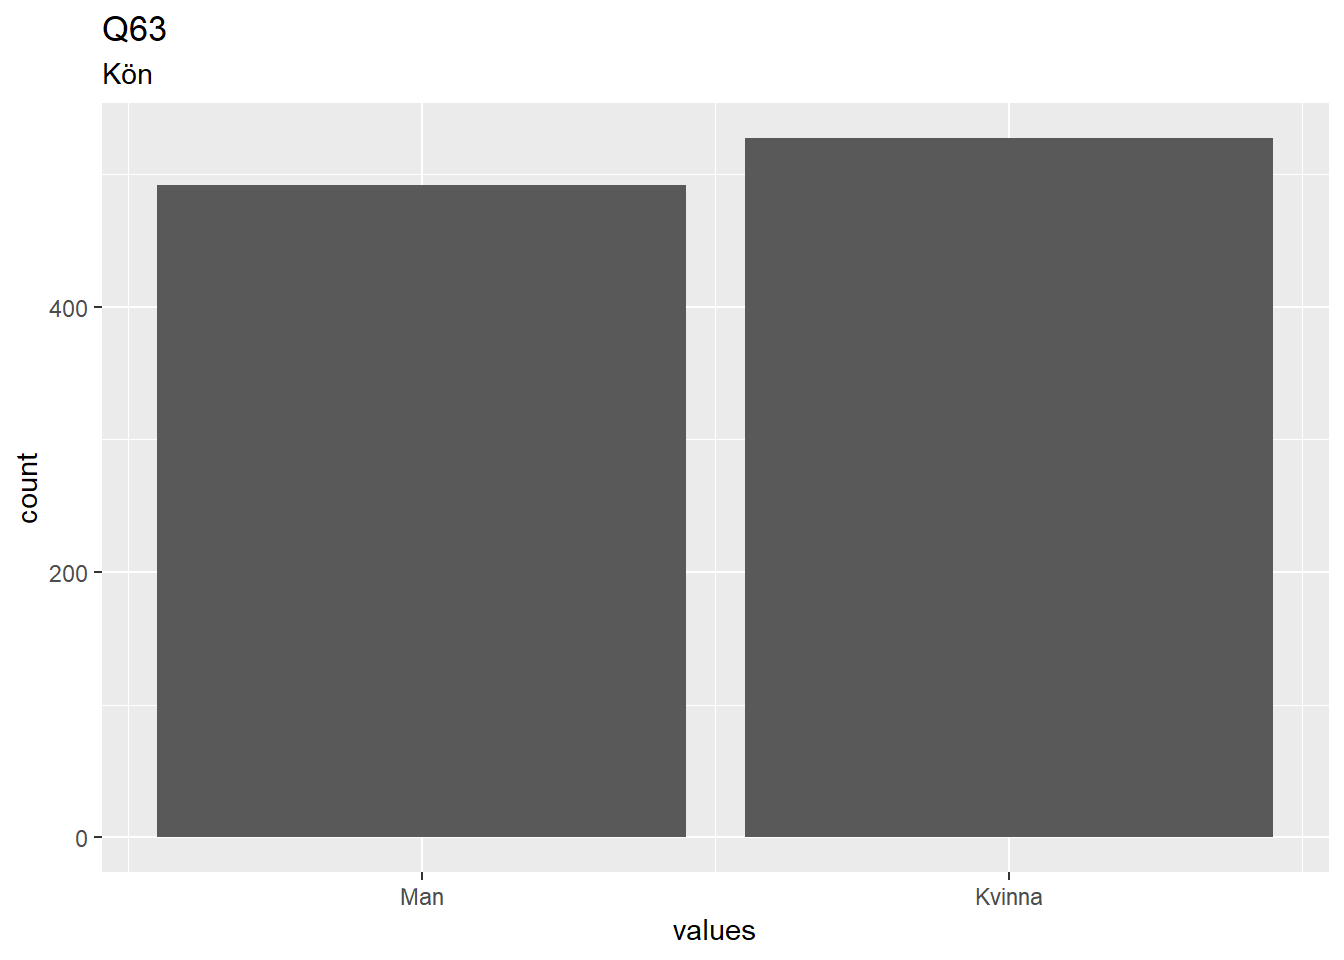
\includegraphics{Goodloser-appendix_files/figure-latex/Q63_distribution-1.pdf}

\begin{Shaded}
\begin{Highlighting}[]
\NormalTok{knitr}\OperatorTok{::}\NormalTok{opts_chunk}\OperatorTok{$}\KeywordTok{set}\NormalTok{(}\DataTypeTok{fig.height =}\NormalTok{ old_height)}
\end{Highlighting}
\end{Shaded}

0 missings.

\subsubsection{Summary statistics}\label{Q63_summary}

\begin{Shaded}
\begin{Highlighting}[]
\KeywordTok{attributes}\NormalTok{(item) <-}\StringTok{ }\NormalTok{item_attributes}
\NormalTok{df =}\StringTok{ }\KeywordTok{data.frame}\NormalTok{(item, }\DataTypeTok{stringsAsFactors =} \OtherTok{FALSE}\NormalTok{)}
\KeywordTok{names}\NormalTok{(df) =}\StringTok{ }\NormalTok{html_item_name}
\KeywordTok{escaped_table}\NormalTok{(}\KeywordTok{codebook_table}\NormalTok{(df))}
\end{Highlighting}
\end{Shaded}

name

label

data\_type

value\_labels

missing

complete

n

mean

sd

p0

p25

p50

p75

p100

hist

format.spss

display\_width

Q63

Kön

numeric

\begin{enumerate}
\def\labelenumi{\arabic{enumi}.}
\tightlist
\item
  Man,2. Kvinna

  0

  1019

  1019

  1.52

  0.5

  1

  1

  2

  2

  2

  ▇▁▁▁▁▁▁▇

  F1.0

  12
\end{enumerate}

\begin{Shaded}
\begin{Highlighting}[]
\ControlFlowTok{if}\NormalTok{ (show_missings) \{}
  \KeywordTok{plot_labelled}\NormalTok{(missings, item_name, wrap_at)}
\NormalTok{\}}
\end{Highlighting}
\end{Shaded}

\begin{Shaded}
\begin{Highlighting}[]
\ControlFlowTok{if}\NormalTok{ (}\OperatorTok{!}\KeywordTok{is.null}\NormalTok{(item_info)) \{}
  \CommentTok{# don't show choices again, if they're basically same thing as value labels}
  \ControlFlowTok{if}\NormalTok{ (}\OperatorTok{!}\KeywordTok{is.null}\NormalTok{(choices) }\OperatorTok{&&}\StringTok{ }\OperatorTok{!}\KeywordTok{is.null}\NormalTok{(item_info}\OperatorTok{$}\NormalTok{choices) }\OperatorTok{&&}\StringTok{ }
\StringTok{    }\KeywordTok{all}\NormalTok{(}\KeywordTok{names}\NormalTok{(}\KeywordTok{na.omit}\NormalTok{(choices)) }\OperatorTok{==}\StringTok{ }\NormalTok{item_info}\OperatorTok{$}\NormalTok{choices) }\OperatorTok{&&}
\StringTok{    }\KeywordTok{all}\NormalTok{(}\KeywordTok{na.omit}\NormalTok{(choices) }\OperatorTok{==}\StringTok{ }\KeywordTok{names}\NormalTok{(item_info}\OperatorTok{$}\NormalTok{choices))) \{}
\NormalTok{    item_info}\OperatorTok{$}\NormalTok{choices <-}\StringTok{ }\OtherTok{NULL}
\NormalTok{  \}}
\NormalTok{  item_info}\OperatorTok{$}\NormalTok{label_parsed <-}\StringTok{ }
\StringTok{    }\NormalTok{item_info}\OperatorTok{$}\NormalTok{choice_list <-}\StringTok{ }\NormalTok{item_info}\OperatorTok{$}\NormalTok{study_id <-}\StringTok{ }\NormalTok{item_info}\OperatorTok{$}\NormalTok{id <-}\StringTok{ }\OtherTok{NULL}
\NormalTok{  pander}\OperatorTok{::}\KeywordTok{pander}\NormalTok{(item_info)}
\NormalTok{\}}
\end{Highlighting}
\end{Shaded}

\subsubsection{Value labels}\label{Q63_labels}

\begin{Shaded}
\begin{Highlighting}[]
\ControlFlowTok{if}\NormalTok{ (}\OperatorTok{!}\KeywordTok{is.null}\NormalTok{(choices) }\OperatorTok{&&}\StringTok{ }\KeywordTok{length}\NormalTok{(choices) }\OperatorTok{&&}\StringTok{ }\KeywordTok{length}\NormalTok{(choices) }\OperatorTok{<}\StringTok{ }\DecValTok{30}\NormalTok{) \{}
\NormalTok{    pander}\OperatorTok{::}\KeywordTok{pander}\NormalTok{(}\KeywordTok{as.list}\NormalTok{(choices))}
\NormalTok{\}}
\end{Highlighting}
\end{Shaded}

\begin{itemize}
\tightlist
\item
  \textbf{Man}: \emph{1}
\item
  \textbf{Kvinna}: \emph{2}
\end{itemize}

\subsection{S3\_1\_1}\label{S3_1_1}

I debatten diskuteras ibland att kommunerna skall kunna förbjuda tiggeri
inom sina gränser. Vad tycker du själv om att förbjuda tiggeri i
kommunen där du bor?

\subsubsection{Distribution}\label{S3_1_1_distribution}

\begin{Shaded}
\begin{Highlighting}[]
\NormalTok{show_missings <-}\StringTok{ }\OtherTok{FALSE}
\ControlFlowTok{if}\NormalTok{ (}\KeywordTok{has_label}\NormalTok{(item)) \{}
\NormalTok{  missings <-}\StringTok{ }\NormalTok{item[}\KeywordTok{is.na}\NormalTok{(haven}\OperatorTok{::}\KeywordTok{zap_missing}\NormalTok{(item))]}
  \KeywordTok{attributes}\NormalTok{(missings) <-}\StringTok{ }\KeywordTok{attributes}\NormalTok{(item)}
  \ControlFlowTok{if}\NormalTok{ (}\OperatorTok{!}\KeywordTok{is.null}\NormalTok{(}\KeywordTok{attributes}\NormalTok{(item)}\OperatorTok{$}\NormalTok{labels)) \{}
    \KeywordTok{attributes}\NormalTok{(missings)}\OperatorTok{$}\NormalTok{labels <-}\StringTok{ }\KeywordTok{attributes}\NormalTok{(missings)}\OperatorTok{$}\NormalTok{labels[}\KeywordTok{is.na}\NormalTok{(}\KeywordTok{attributes}\NormalTok{(missings)}\OperatorTok{$}\NormalTok{labels)]}
    \KeywordTok{attributes}\NormalTok{(item)}\OperatorTok{$}\NormalTok{labels <-}\StringTok{ }\KeywordTok{attributes}\NormalTok{(item)}\OperatorTok{$}\NormalTok{labels[}\OperatorTok{!}\KeywordTok{is.na}\NormalTok{(}\KeywordTok{attributes}\NormalTok{(item)}\OperatorTok{$}\NormalTok{labels)]}
\NormalTok{  \}}
  \ControlFlowTok{if}\NormalTok{ (}\KeywordTok{is.numeric}\NormalTok{(item)) \{}
\NormalTok{    show_missings <-}\StringTok{ }\KeywordTok{length}\NormalTok{(}\KeywordTok{unique}\NormalTok{(haven}\OperatorTok{::}\KeywordTok{na_tag}\NormalTok{(missings))) }\OperatorTok{>}\StringTok{ }\DecValTok{1}
\NormalTok{    item <-}\StringTok{ }\NormalTok{haven}\OperatorTok{::}\KeywordTok{zap_missing}\NormalTok{(item)}
\NormalTok{  \}}
  \ControlFlowTok{if}\NormalTok{ (}\KeywordTok{length}\NormalTok{(item_attributes}\OperatorTok{$}\NormalTok{labels) }\OperatorTok{==}\StringTok{ }\DecValTok{0} \OperatorTok{&&}\StringTok{ }\KeywordTok{is.numeric}\NormalTok{(item)) \{}
\NormalTok{    item <-}\StringTok{ }\NormalTok{haven}\OperatorTok{::}\KeywordTok{zap_labels}\NormalTok{(item)}
\NormalTok{  \}}
\NormalTok{\}}
\NormalTok{item_nomiss <-}\StringTok{ }\NormalTok{item[}\OperatorTok{!}\KeywordTok{is.na}\NormalTok{(item)]}

\CommentTok{# unnest mc_multiple and so on}
\ControlFlowTok{if}\NormalTok{ (}
  \KeywordTok{is.character}\NormalTok{(item_nomiss) }\OperatorTok{&&}
\StringTok{  }\NormalTok{stringr}\OperatorTok{::}\KeywordTok{str_detect}\NormalTok{(item_nomiss, stringr}\OperatorTok{::}\KeywordTok{fixed}\NormalTok{(}\StringTok{", "}\NormalTok{)) }\OperatorTok{&&}
\StringTok{  }\NormalTok{(}\KeywordTok{exists}\NormalTok{(}\StringTok{"type"}\NormalTok{, item_info) }\OperatorTok{&&}\StringTok{ }
\StringTok{    }\NormalTok{stringr}\OperatorTok{::}\KeywordTok{str_detect}\NormalTok{(item_info}\OperatorTok{$}\NormalTok{type, }\DataTypeTok{pattern =}\NormalTok{ stringr}\OperatorTok{::}\KeywordTok{fixed}\NormalTok{(}\StringTok{"multiple"}\NormalTok{)))}
\NormalTok{  ) \{}
\NormalTok{  item_nomiss <-}\StringTok{ }\KeywordTok{unlist}\NormalTok{(stringr}\OperatorTok{::}\KeywordTok{str_split}\NormalTok{(item_nomiss, }\DataTypeTok{pattern =}\NormalTok{ stringr}\OperatorTok{::}\KeywordTok{fixed}\NormalTok{(}\StringTok{", "}\NormalTok{)))}
\NormalTok{\}}
\KeywordTok{attributes}\NormalTok{(item_nomiss) <-}\StringTok{ }\KeywordTok{attributes}\NormalTok{(item)}

\NormalTok{old_height <-}\StringTok{ }\NormalTok{knitr}\OperatorTok{::}\NormalTok{opts_chunk}\OperatorTok{$}\KeywordTok{get}\NormalTok{(}\StringTok{"fig.height"}\NormalTok{)}
\NormalTok{non_missing_choices <-}\StringTok{ }\NormalTok{item_attributes[[}\StringTok{"labels"}\NormalTok{]]}
\NormalTok{many_labels <-}\StringTok{ }\KeywordTok{length}\NormalTok{(non_missing_choices) }\OperatorTok{>}\StringTok{ }\DecValTok{7}
\NormalTok{go_vertical <-}\StringTok{ }\OperatorTok{!}\KeywordTok{is.numeric}\NormalTok{(item_nomiss) }\OperatorTok{||}\StringTok{ }\NormalTok{many_labels}
\ControlFlowTok{if}\NormalTok{ ( go_vertical ) \{}
  \CommentTok{# numeric items are plotted horizontally (because that's what usually expected)}
  \CommentTok{# categorical items are plotted vertically because we can use the screen real estate better this way}

    \ControlFlowTok{if}\NormalTok{ (}\KeywordTok{is.null}\NormalTok{(choices) }\OperatorTok{||}\StringTok{ }
\StringTok{        }\NormalTok{dplyr}\OperatorTok{::}\KeywordTok{n_distinct}\NormalTok{(item_nomiss) }\OperatorTok{>}\StringTok{ }\KeywordTok{length}\NormalTok{(non_missing_choices)) \{}
\NormalTok{        non_missing_choices <-}\StringTok{ }\KeywordTok{unique}\NormalTok{(item_nomiss)}
        \KeywordTok{names}\NormalTok{(non_missing_choices) <-}\StringTok{ }\NormalTok{non_missing_choices}
\NormalTok{    \}}
\NormalTok{  choice_multiplier <-}\StringTok{ }\NormalTok{old_height}\OperatorTok{/}\FloatTok{6.5}
\NormalTok{    new_height <-}\StringTok{ }\DecValTok{2} \OperatorTok{+}\StringTok{ }\NormalTok{choice_multiplier }\OperatorTok{*}\StringTok{ }\KeywordTok{length}\NormalTok{(non_missing_choices)}
\NormalTok{    new_height <-}\StringTok{ }\KeywordTok{ifelse}\NormalTok{(new_height }\OperatorTok{>}\StringTok{ }\DecValTok{20}\NormalTok{, }\DecValTok{20}\NormalTok{, new_height)}
\NormalTok{    new_height <-}\StringTok{ }\KeywordTok{ifelse}\NormalTok{(new_height }\OperatorTok{<}\StringTok{ }\DecValTok{1}\NormalTok{, }\DecValTok{1}\NormalTok{, new_height)}
\NormalTok{    knitr}\OperatorTok{::}\NormalTok{opts_chunk}\OperatorTok{$}\KeywordTok{set}\NormalTok{(}\DataTypeTok{fig.height =}\NormalTok{ new_height)}
\NormalTok{\}}

\NormalTok{wrap_at <-}\StringTok{ }\NormalTok{knitr}\OperatorTok{::}\NormalTok{opts_chunk}\OperatorTok{$}\KeywordTok{get}\NormalTok{(}\StringTok{"fig.width"}\NormalTok{) }\OperatorTok{*}\StringTok{ }\DecValTok{10}
\end{Highlighting}
\end{Shaded}

\begin{Shaded}
\begin{Highlighting}[]
\CommentTok{# todo: if there are free-text choices mingled in with the pre-defined ones, don't show}
\CommentTok{# todo: show rare items if they are pre-defined}
\CommentTok{# todo: bin rare responses into "other category"}
\ControlFlowTok{if}\NormalTok{ (}\OperatorTok{!}\KeywordTok{length}\NormalTok{(item_nomiss)) \{}
  \KeywordTok{cat}\NormalTok{(}\StringTok{"No non-missing values to show."}\NormalTok{)}
\NormalTok{\} }\ControlFlowTok{else} \ControlFlowTok{if}\NormalTok{ (}\KeywordTok{is.numeric}\NormalTok{(item_nomiss) }\OperatorTok{||}\StringTok{ }\NormalTok{dplyr}\OperatorTok{::}\KeywordTok{n_distinct}\NormalTok{(item_nomiss) }\OperatorTok{<}\StringTok{ }\DecValTok{20}\NormalTok{) \{}
  \KeywordTok{plot_labelled}\NormalTok{(item_nomiss, item_name, wrap_at, go_vertical)}
\NormalTok{\} }\ControlFlowTok{else}\NormalTok{ \{}
    \KeywordTok{cat}\NormalTok{(dplyr}\OperatorTok{::}\KeywordTok{n_distinct}\NormalTok{(item_nomiss), }\StringTok{" unique, categorical values, so not shown."}\NormalTok{)}
\NormalTok{\}}
\end{Highlighting}
\end{Shaded}

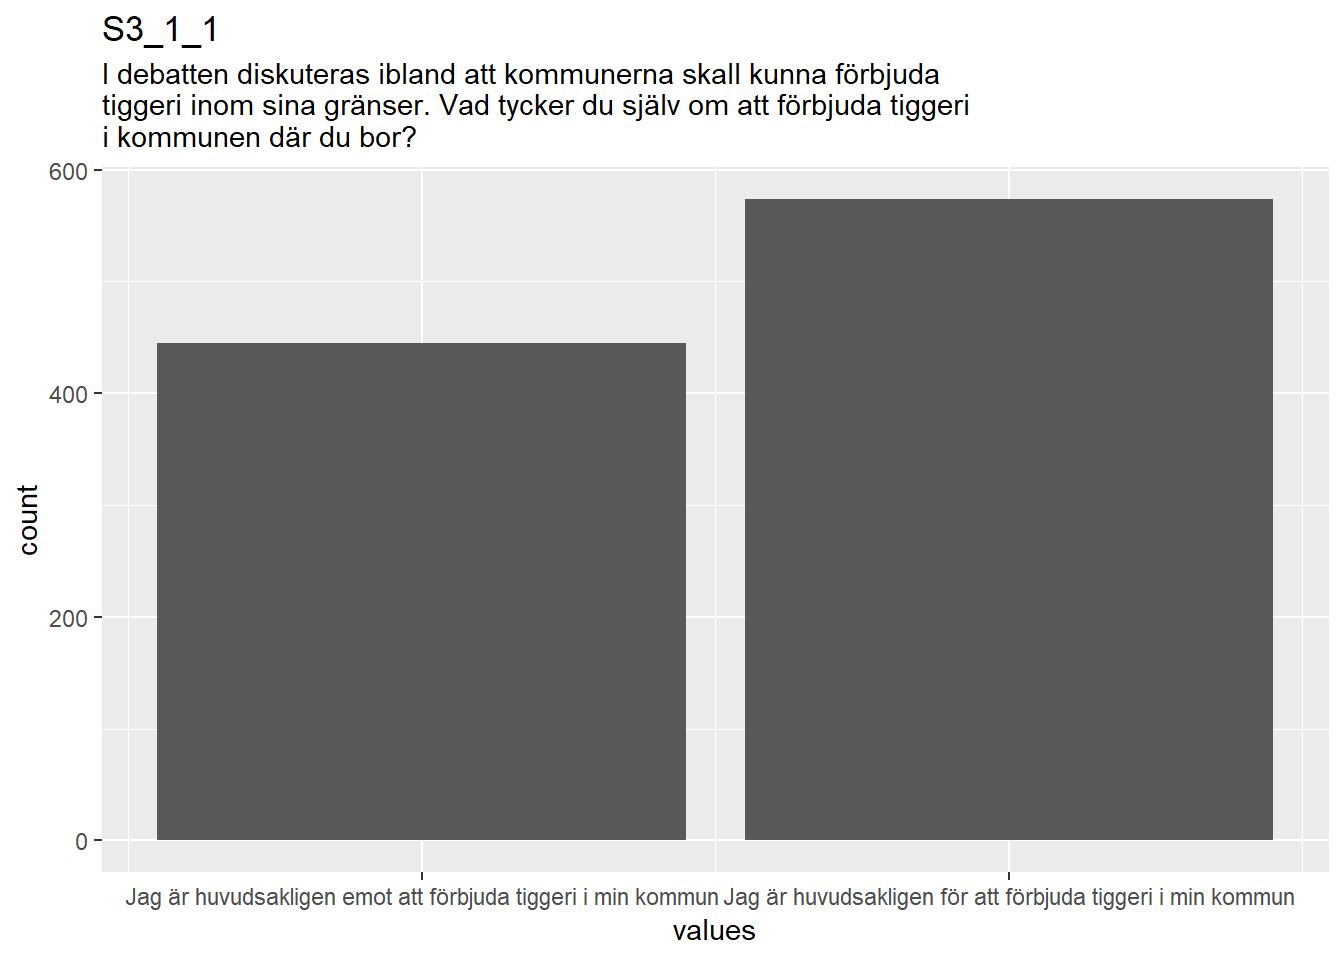
\includegraphics{Goodloser-appendix_files/figure-latex/S3_1_1_distribution-1.pdf}

\begin{Shaded}
\begin{Highlighting}[]
\NormalTok{knitr}\OperatorTok{::}\NormalTok{opts_chunk}\OperatorTok{$}\KeywordTok{set}\NormalTok{(}\DataTypeTok{fig.height =}\NormalTok{ old_height)}
\end{Highlighting}
\end{Shaded}

0 missings.

\subsubsection{Summary statistics}\label{S3_1_1_summary}

\begin{Shaded}
\begin{Highlighting}[]
\KeywordTok{attributes}\NormalTok{(item) <-}\StringTok{ }\NormalTok{item_attributes}
\NormalTok{df =}\StringTok{ }\KeywordTok{data.frame}\NormalTok{(item, }\DataTypeTok{stringsAsFactors =} \OtherTok{FALSE}\NormalTok{)}
\KeywordTok{names}\NormalTok{(df) =}\StringTok{ }\NormalTok{html_item_name}
\KeywordTok{escaped_table}\NormalTok{(}\KeywordTok{codebook_table}\NormalTok{(df))}
\end{Highlighting}
\end{Shaded}

name

label

data\_type

value\_labels

missing

complete

n

mean

sd

p0

p25

p50

p75

p100

hist

format.spss

display\_width

S3\_1\_1

I debatten diskuteras ibland att kommunerna skall kunna förbjuda tiggeri
inom sina gränser. Vad tycker du själv om att förbjuda tiggeri i
kommunen där du bor?

numeric

\begin{enumerate}
\def\labelenumi{\arabic{enumi}.}
\tightlist
\item
  Jag är huvudsakligen emot att förbjuda tiggeri i min kommun,2. Jag är
  huvudsakligen för att förbjuda tiggeri i min kommun

  0

  1019

  1019

  1.56

  0.5

  1

  1

  2

  2

  2

  ▆▁▁▁▁▁▁▇

  F1.0

  12
\end{enumerate}

\begin{Shaded}
\begin{Highlighting}[]
\ControlFlowTok{if}\NormalTok{ (show_missings) \{}
  \KeywordTok{plot_labelled}\NormalTok{(missings, item_name, wrap_at)}
\NormalTok{\}}
\end{Highlighting}
\end{Shaded}

\begin{Shaded}
\begin{Highlighting}[]
\ControlFlowTok{if}\NormalTok{ (}\OperatorTok{!}\KeywordTok{is.null}\NormalTok{(item_info)) \{}
  \CommentTok{# don't show choices again, if they're basically same thing as value labels}
  \ControlFlowTok{if}\NormalTok{ (}\OperatorTok{!}\KeywordTok{is.null}\NormalTok{(choices) }\OperatorTok{&&}\StringTok{ }\OperatorTok{!}\KeywordTok{is.null}\NormalTok{(item_info}\OperatorTok{$}\NormalTok{choices) }\OperatorTok{&&}\StringTok{ }
\StringTok{    }\KeywordTok{all}\NormalTok{(}\KeywordTok{names}\NormalTok{(}\KeywordTok{na.omit}\NormalTok{(choices)) }\OperatorTok{==}\StringTok{ }\NormalTok{item_info}\OperatorTok{$}\NormalTok{choices) }\OperatorTok{&&}
\StringTok{    }\KeywordTok{all}\NormalTok{(}\KeywordTok{na.omit}\NormalTok{(choices) }\OperatorTok{==}\StringTok{ }\KeywordTok{names}\NormalTok{(item_info}\OperatorTok{$}\NormalTok{choices))) \{}
\NormalTok{    item_info}\OperatorTok{$}\NormalTok{choices <-}\StringTok{ }\OtherTok{NULL}
\NormalTok{  \}}
\NormalTok{  item_info}\OperatorTok{$}\NormalTok{label_parsed <-}\StringTok{ }
\StringTok{    }\NormalTok{item_info}\OperatorTok{$}\NormalTok{choice_list <-}\StringTok{ }\NormalTok{item_info}\OperatorTok{$}\NormalTok{study_id <-}\StringTok{ }\NormalTok{item_info}\OperatorTok{$}\NormalTok{id <-}\StringTok{ }\OtherTok{NULL}
\NormalTok{  pander}\OperatorTok{::}\KeywordTok{pander}\NormalTok{(item_info)}
\NormalTok{\}}
\end{Highlighting}
\end{Shaded}

\subsubsection{Value labels}\label{S3_1_1_labels}

\begin{Shaded}
\begin{Highlighting}[]
\ControlFlowTok{if}\NormalTok{ (}\OperatorTok{!}\KeywordTok{is.null}\NormalTok{(choices) }\OperatorTok{&&}\StringTok{ }\KeywordTok{length}\NormalTok{(choices) }\OperatorTok{&&}\StringTok{ }\KeywordTok{length}\NormalTok{(choices) }\OperatorTok{<}\StringTok{ }\DecValTok{30}\NormalTok{) \{}
\NormalTok{    pander}\OperatorTok{::}\KeywordTok{pander}\NormalTok{(}\KeywordTok{as.list}\NormalTok{(choices))}
\NormalTok{\}}
\end{Highlighting}
\end{Shaded}

\begin{itemize}
\tightlist
\item
  \textbf{Jag är huvudsakligen emot att förbjuda tiggeri i min kommun}:
  \emph{1}
\item
  \textbf{Jag är huvudsakligen för att förbjuda tiggeri i min kommun}:
  \emph{2}
\end{itemize}

\subsection{S3\_2\_1}\label{S3_2_1}

Hur viktig är frågan för dig personligen?

\subsubsection{Distribution}\label{S3_2_1_distribution}

\begin{Shaded}
\begin{Highlighting}[]
\NormalTok{show_missings <-}\StringTok{ }\OtherTok{FALSE}
\ControlFlowTok{if}\NormalTok{ (}\KeywordTok{has_label}\NormalTok{(item)) \{}
\NormalTok{  missings <-}\StringTok{ }\NormalTok{item[}\KeywordTok{is.na}\NormalTok{(haven}\OperatorTok{::}\KeywordTok{zap_missing}\NormalTok{(item))]}
  \KeywordTok{attributes}\NormalTok{(missings) <-}\StringTok{ }\KeywordTok{attributes}\NormalTok{(item)}
  \ControlFlowTok{if}\NormalTok{ (}\OperatorTok{!}\KeywordTok{is.null}\NormalTok{(}\KeywordTok{attributes}\NormalTok{(item)}\OperatorTok{$}\NormalTok{labels)) \{}
    \KeywordTok{attributes}\NormalTok{(missings)}\OperatorTok{$}\NormalTok{labels <-}\StringTok{ }\KeywordTok{attributes}\NormalTok{(missings)}\OperatorTok{$}\NormalTok{labels[}\KeywordTok{is.na}\NormalTok{(}\KeywordTok{attributes}\NormalTok{(missings)}\OperatorTok{$}\NormalTok{labels)]}
    \KeywordTok{attributes}\NormalTok{(item)}\OperatorTok{$}\NormalTok{labels <-}\StringTok{ }\KeywordTok{attributes}\NormalTok{(item)}\OperatorTok{$}\NormalTok{labels[}\OperatorTok{!}\KeywordTok{is.na}\NormalTok{(}\KeywordTok{attributes}\NormalTok{(item)}\OperatorTok{$}\NormalTok{labels)]}
\NormalTok{  \}}
  \ControlFlowTok{if}\NormalTok{ (}\KeywordTok{is.numeric}\NormalTok{(item)) \{}
\NormalTok{    show_missings <-}\StringTok{ }\KeywordTok{length}\NormalTok{(}\KeywordTok{unique}\NormalTok{(haven}\OperatorTok{::}\KeywordTok{na_tag}\NormalTok{(missings))) }\OperatorTok{>}\StringTok{ }\DecValTok{1}
\NormalTok{    item <-}\StringTok{ }\NormalTok{haven}\OperatorTok{::}\KeywordTok{zap_missing}\NormalTok{(item)}
\NormalTok{  \}}
  \ControlFlowTok{if}\NormalTok{ (}\KeywordTok{length}\NormalTok{(item_attributes}\OperatorTok{$}\NormalTok{labels) }\OperatorTok{==}\StringTok{ }\DecValTok{0} \OperatorTok{&&}\StringTok{ }\KeywordTok{is.numeric}\NormalTok{(item)) \{}
\NormalTok{    item <-}\StringTok{ }\NormalTok{haven}\OperatorTok{::}\KeywordTok{zap_labels}\NormalTok{(item)}
\NormalTok{  \}}
\NormalTok{\}}
\NormalTok{item_nomiss <-}\StringTok{ }\NormalTok{item[}\OperatorTok{!}\KeywordTok{is.na}\NormalTok{(item)]}

\CommentTok{# unnest mc_multiple and so on}
\ControlFlowTok{if}\NormalTok{ (}
  \KeywordTok{is.character}\NormalTok{(item_nomiss) }\OperatorTok{&&}
\StringTok{  }\NormalTok{stringr}\OperatorTok{::}\KeywordTok{str_detect}\NormalTok{(item_nomiss, stringr}\OperatorTok{::}\KeywordTok{fixed}\NormalTok{(}\StringTok{", "}\NormalTok{)) }\OperatorTok{&&}
\StringTok{  }\NormalTok{(}\KeywordTok{exists}\NormalTok{(}\StringTok{"type"}\NormalTok{, item_info) }\OperatorTok{&&}\StringTok{ }
\StringTok{    }\NormalTok{stringr}\OperatorTok{::}\KeywordTok{str_detect}\NormalTok{(item_info}\OperatorTok{$}\NormalTok{type, }\DataTypeTok{pattern =}\NormalTok{ stringr}\OperatorTok{::}\KeywordTok{fixed}\NormalTok{(}\StringTok{"multiple"}\NormalTok{)))}
\NormalTok{  ) \{}
\NormalTok{  item_nomiss <-}\StringTok{ }\KeywordTok{unlist}\NormalTok{(stringr}\OperatorTok{::}\KeywordTok{str_split}\NormalTok{(item_nomiss, }\DataTypeTok{pattern =}\NormalTok{ stringr}\OperatorTok{::}\KeywordTok{fixed}\NormalTok{(}\StringTok{", "}\NormalTok{)))}
\NormalTok{\}}
\KeywordTok{attributes}\NormalTok{(item_nomiss) <-}\StringTok{ }\KeywordTok{attributes}\NormalTok{(item)}

\NormalTok{old_height <-}\StringTok{ }\NormalTok{knitr}\OperatorTok{::}\NormalTok{opts_chunk}\OperatorTok{$}\KeywordTok{get}\NormalTok{(}\StringTok{"fig.height"}\NormalTok{)}
\NormalTok{non_missing_choices <-}\StringTok{ }\NormalTok{item_attributes[[}\StringTok{"labels"}\NormalTok{]]}
\NormalTok{many_labels <-}\StringTok{ }\KeywordTok{length}\NormalTok{(non_missing_choices) }\OperatorTok{>}\StringTok{ }\DecValTok{7}
\NormalTok{go_vertical <-}\StringTok{ }\OperatorTok{!}\KeywordTok{is.numeric}\NormalTok{(item_nomiss) }\OperatorTok{||}\StringTok{ }\NormalTok{many_labels}
\ControlFlowTok{if}\NormalTok{ ( go_vertical ) \{}
  \CommentTok{# numeric items are plotted horizontally (because that's what usually expected)}
  \CommentTok{# categorical items are plotted vertically because we can use the screen real estate better this way}

    \ControlFlowTok{if}\NormalTok{ (}\KeywordTok{is.null}\NormalTok{(choices) }\OperatorTok{||}\StringTok{ }
\StringTok{        }\NormalTok{dplyr}\OperatorTok{::}\KeywordTok{n_distinct}\NormalTok{(item_nomiss) }\OperatorTok{>}\StringTok{ }\KeywordTok{length}\NormalTok{(non_missing_choices)) \{}
\NormalTok{        non_missing_choices <-}\StringTok{ }\KeywordTok{unique}\NormalTok{(item_nomiss)}
        \KeywordTok{names}\NormalTok{(non_missing_choices) <-}\StringTok{ }\NormalTok{non_missing_choices}
\NormalTok{    \}}
\NormalTok{  choice_multiplier <-}\StringTok{ }\NormalTok{old_height}\OperatorTok{/}\FloatTok{6.5}
\NormalTok{    new_height <-}\StringTok{ }\DecValTok{2} \OperatorTok{+}\StringTok{ }\NormalTok{choice_multiplier }\OperatorTok{*}\StringTok{ }\KeywordTok{length}\NormalTok{(non_missing_choices)}
\NormalTok{    new_height <-}\StringTok{ }\KeywordTok{ifelse}\NormalTok{(new_height }\OperatorTok{>}\StringTok{ }\DecValTok{20}\NormalTok{, }\DecValTok{20}\NormalTok{, new_height)}
\NormalTok{    new_height <-}\StringTok{ }\KeywordTok{ifelse}\NormalTok{(new_height }\OperatorTok{<}\StringTok{ }\DecValTok{1}\NormalTok{, }\DecValTok{1}\NormalTok{, new_height)}
\NormalTok{    knitr}\OperatorTok{::}\NormalTok{opts_chunk}\OperatorTok{$}\KeywordTok{set}\NormalTok{(}\DataTypeTok{fig.height =}\NormalTok{ new_height)}
\NormalTok{\}}

\NormalTok{wrap_at <-}\StringTok{ }\NormalTok{knitr}\OperatorTok{::}\NormalTok{opts_chunk}\OperatorTok{$}\KeywordTok{get}\NormalTok{(}\StringTok{"fig.width"}\NormalTok{) }\OperatorTok{*}\StringTok{ }\DecValTok{10}
\end{Highlighting}
\end{Shaded}

\begin{Shaded}
\begin{Highlighting}[]
\CommentTok{# todo: if there are free-text choices mingled in with the pre-defined ones, don't show}
\CommentTok{# todo: show rare items if they are pre-defined}
\CommentTok{# todo: bin rare responses into "other category"}
\ControlFlowTok{if}\NormalTok{ (}\OperatorTok{!}\KeywordTok{length}\NormalTok{(item_nomiss)) \{}
  \KeywordTok{cat}\NormalTok{(}\StringTok{"No non-missing values to show."}\NormalTok{)}
\NormalTok{\} }\ControlFlowTok{else} \ControlFlowTok{if}\NormalTok{ (}\KeywordTok{is.numeric}\NormalTok{(item_nomiss) }\OperatorTok{||}\StringTok{ }\NormalTok{dplyr}\OperatorTok{::}\KeywordTok{n_distinct}\NormalTok{(item_nomiss) }\OperatorTok{<}\StringTok{ }\DecValTok{20}\NormalTok{) \{}
  \KeywordTok{plot_labelled}\NormalTok{(item_nomiss, item_name, wrap_at, go_vertical)}
\NormalTok{\} }\ControlFlowTok{else}\NormalTok{ \{}
    \KeywordTok{cat}\NormalTok{(dplyr}\OperatorTok{::}\KeywordTok{n_distinct}\NormalTok{(item_nomiss), }\StringTok{" unique, categorical values, so not shown."}\NormalTok{)}
\NormalTok{\}}
\end{Highlighting}
\end{Shaded}

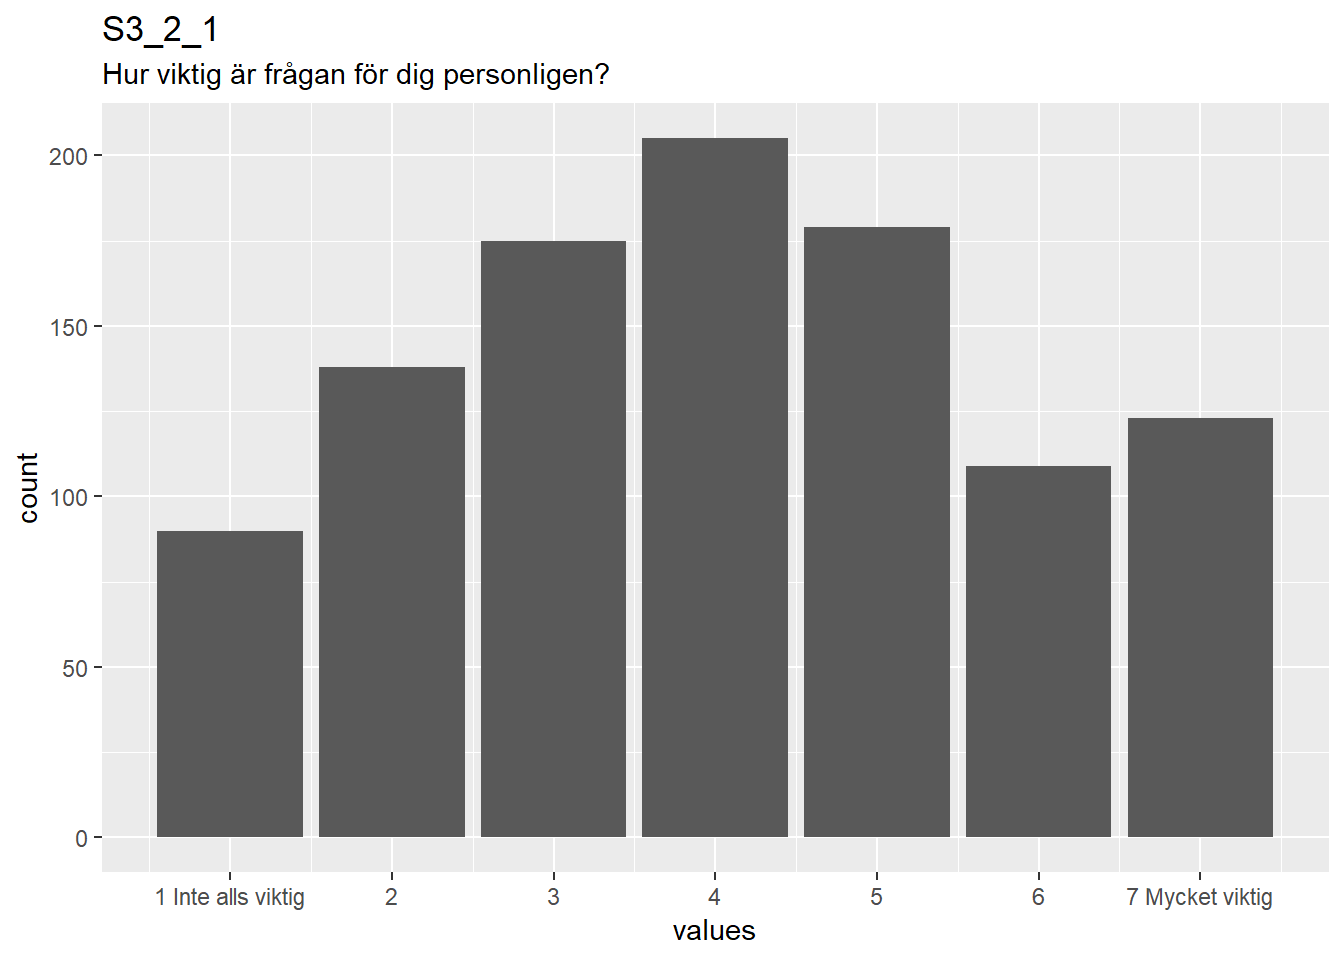
\includegraphics{Goodloser-appendix_files/figure-latex/S3_2_1_distribution-1.pdf}

\begin{Shaded}
\begin{Highlighting}[]
\NormalTok{knitr}\OperatorTok{::}\NormalTok{opts_chunk}\OperatorTok{$}\KeywordTok{set}\NormalTok{(}\DataTypeTok{fig.height =}\NormalTok{ old_height)}
\end{Highlighting}
\end{Shaded}

0 missings.

\subsubsection{Summary statistics}\label{S3_2_1_summary}

\begin{Shaded}
\begin{Highlighting}[]
\KeywordTok{attributes}\NormalTok{(item) <-}\StringTok{ }\NormalTok{item_attributes}
\NormalTok{df =}\StringTok{ }\KeywordTok{data.frame}\NormalTok{(item, }\DataTypeTok{stringsAsFactors =} \OtherTok{FALSE}\NormalTok{)}
\KeywordTok{names}\NormalTok{(df) =}\StringTok{ }\NormalTok{html_item_name}
\KeywordTok{escaped_table}\NormalTok{(}\KeywordTok{codebook_table}\NormalTok{(df))}
\end{Highlighting}
\end{Shaded}

name

label

data\_type

value\_labels

missing

complete

n

mean

sd

p0

p25

p50

p75

p100

hist

format.spss

display\_width

S3\_2\_1

Hur viktig är frågan för dig personligen?

numeric

\begin{enumerate}
\def\labelenumi{\arabic{enumi}.}
\tightlist
\item
  1 Inte alls viktig,2. 2,3. 3,4. 4,5. 5,6. 6,7. 7 Mycket viktig

  0

  1019

  1019

  4.04

  1.79

  1

  3

  4

  5

  7

  ▃▆▇▇▁▇▅▅

  F1.0

  12
\end{enumerate}

\begin{Shaded}
\begin{Highlighting}[]
\ControlFlowTok{if}\NormalTok{ (show_missings) \{}
  \KeywordTok{plot_labelled}\NormalTok{(missings, item_name, wrap_at)}
\NormalTok{\}}
\end{Highlighting}
\end{Shaded}

\begin{Shaded}
\begin{Highlighting}[]
\ControlFlowTok{if}\NormalTok{ (}\OperatorTok{!}\KeywordTok{is.null}\NormalTok{(item_info)) \{}
  \CommentTok{# don't show choices again, if they're basically same thing as value labels}
  \ControlFlowTok{if}\NormalTok{ (}\OperatorTok{!}\KeywordTok{is.null}\NormalTok{(choices) }\OperatorTok{&&}\StringTok{ }\OperatorTok{!}\KeywordTok{is.null}\NormalTok{(item_info}\OperatorTok{$}\NormalTok{choices) }\OperatorTok{&&}\StringTok{ }
\StringTok{    }\KeywordTok{all}\NormalTok{(}\KeywordTok{names}\NormalTok{(}\KeywordTok{na.omit}\NormalTok{(choices)) }\OperatorTok{==}\StringTok{ }\NormalTok{item_info}\OperatorTok{$}\NormalTok{choices) }\OperatorTok{&&}
\StringTok{    }\KeywordTok{all}\NormalTok{(}\KeywordTok{na.omit}\NormalTok{(choices) }\OperatorTok{==}\StringTok{ }\KeywordTok{names}\NormalTok{(item_info}\OperatorTok{$}\NormalTok{choices))) \{}
\NormalTok{    item_info}\OperatorTok{$}\NormalTok{choices <-}\StringTok{ }\OtherTok{NULL}
\NormalTok{  \}}
\NormalTok{  item_info}\OperatorTok{$}\NormalTok{label_parsed <-}\StringTok{ }
\StringTok{    }\NormalTok{item_info}\OperatorTok{$}\NormalTok{choice_list <-}\StringTok{ }\NormalTok{item_info}\OperatorTok{$}\NormalTok{study_id <-}\StringTok{ }\NormalTok{item_info}\OperatorTok{$}\NormalTok{id <-}\StringTok{ }\OtherTok{NULL}
\NormalTok{  pander}\OperatorTok{::}\KeywordTok{pander}\NormalTok{(item_info)}
\NormalTok{\}}
\end{Highlighting}
\end{Shaded}

\subsubsection{Value labels}\label{S3_2_1_labels}

\begin{Shaded}
\begin{Highlighting}[]
\ControlFlowTok{if}\NormalTok{ (}\OperatorTok{!}\KeywordTok{is.null}\NormalTok{(choices) }\OperatorTok{&&}\StringTok{ }\KeywordTok{length}\NormalTok{(choices) }\OperatorTok{&&}\StringTok{ }\KeywordTok{length}\NormalTok{(choices) }\OperatorTok{<}\StringTok{ }\DecValTok{30}\NormalTok{) \{}
\NormalTok{    pander}\OperatorTok{::}\KeywordTok{pander}\NormalTok{(}\KeywordTok{as.list}\NormalTok{(choices))}
\NormalTok{\}}
\end{Highlighting}
\end{Shaded}

\begin{itemize}
\tightlist
\item
  \textbf{1 Inte alls viktig}: \emph{1}
\item
  \textbf{2}: \emph{2}
\item
  \textbf{3}: \emph{3}
\item
  \textbf{4}: \emph{4}
\item
  \textbf{5}: \emph{5}
\item
  \textbf{6}: \emph{6}
\item
  \textbf{7 Mycket viktig}: \emph{7}
\end{itemize}

\subsection{S3\_4\_1\_1}\label{S3_4_1_1}

Hur rättvist tycker du att det gick till när det fattades beslut om att
förbjuda tiggeri?

\subsubsection{Distribution}\label{S3_4_1_1_distribution}

\begin{Shaded}
\begin{Highlighting}[]
\NormalTok{show_missings <-}\StringTok{ }\OtherTok{FALSE}
\ControlFlowTok{if}\NormalTok{ (}\KeywordTok{has_label}\NormalTok{(item)) \{}
\NormalTok{  missings <-}\StringTok{ }\NormalTok{item[}\KeywordTok{is.na}\NormalTok{(haven}\OperatorTok{::}\KeywordTok{zap_missing}\NormalTok{(item))]}
  \KeywordTok{attributes}\NormalTok{(missings) <-}\StringTok{ }\KeywordTok{attributes}\NormalTok{(item)}
  \ControlFlowTok{if}\NormalTok{ (}\OperatorTok{!}\KeywordTok{is.null}\NormalTok{(}\KeywordTok{attributes}\NormalTok{(item)}\OperatorTok{$}\NormalTok{labels)) \{}
    \KeywordTok{attributes}\NormalTok{(missings)}\OperatorTok{$}\NormalTok{labels <-}\StringTok{ }\KeywordTok{attributes}\NormalTok{(missings)}\OperatorTok{$}\NormalTok{labels[}\KeywordTok{is.na}\NormalTok{(}\KeywordTok{attributes}\NormalTok{(missings)}\OperatorTok{$}\NormalTok{labels)]}
    \KeywordTok{attributes}\NormalTok{(item)}\OperatorTok{$}\NormalTok{labels <-}\StringTok{ }\KeywordTok{attributes}\NormalTok{(item)}\OperatorTok{$}\NormalTok{labels[}\OperatorTok{!}\KeywordTok{is.na}\NormalTok{(}\KeywordTok{attributes}\NormalTok{(item)}\OperatorTok{$}\NormalTok{labels)]}
\NormalTok{  \}}
  \ControlFlowTok{if}\NormalTok{ (}\KeywordTok{is.numeric}\NormalTok{(item)) \{}
\NormalTok{    show_missings <-}\StringTok{ }\KeywordTok{length}\NormalTok{(}\KeywordTok{unique}\NormalTok{(haven}\OperatorTok{::}\KeywordTok{na_tag}\NormalTok{(missings))) }\OperatorTok{>}\StringTok{ }\DecValTok{1}
\NormalTok{    item <-}\StringTok{ }\NormalTok{haven}\OperatorTok{::}\KeywordTok{zap_missing}\NormalTok{(item)}
\NormalTok{  \}}
  \ControlFlowTok{if}\NormalTok{ (}\KeywordTok{length}\NormalTok{(item_attributes}\OperatorTok{$}\NormalTok{labels) }\OperatorTok{==}\StringTok{ }\DecValTok{0} \OperatorTok{&&}\StringTok{ }\KeywordTok{is.numeric}\NormalTok{(item)) \{}
\NormalTok{    item <-}\StringTok{ }\NormalTok{haven}\OperatorTok{::}\KeywordTok{zap_labels}\NormalTok{(item)}
\NormalTok{  \}}
\NormalTok{\}}
\NormalTok{item_nomiss <-}\StringTok{ }\NormalTok{item[}\OperatorTok{!}\KeywordTok{is.na}\NormalTok{(item)]}

\CommentTok{# unnest mc_multiple and so on}
\ControlFlowTok{if}\NormalTok{ (}
  \KeywordTok{is.character}\NormalTok{(item_nomiss) }\OperatorTok{&&}
\StringTok{  }\NormalTok{stringr}\OperatorTok{::}\KeywordTok{str_detect}\NormalTok{(item_nomiss, stringr}\OperatorTok{::}\KeywordTok{fixed}\NormalTok{(}\StringTok{", "}\NormalTok{)) }\OperatorTok{&&}
\StringTok{  }\NormalTok{(}\KeywordTok{exists}\NormalTok{(}\StringTok{"type"}\NormalTok{, item_info) }\OperatorTok{&&}\StringTok{ }
\StringTok{    }\NormalTok{stringr}\OperatorTok{::}\KeywordTok{str_detect}\NormalTok{(item_info}\OperatorTok{$}\NormalTok{type, }\DataTypeTok{pattern =}\NormalTok{ stringr}\OperatorTok{::}\KeywordTok{fixed}\NormalTok{(}\StringTok{"multiple"}\NormalTok{)))}
\NormalTok{  ) \{}
\NormalTok{  item_nomiss <-}\StringTok{ }\KeywordTok{unlist}\NormalTok{(stringr}\OperatorTok{::}\KeywordTok{str_split}\NormalTok{(item_nomiss, }\DataTypeTok{pattern =}\NormalTok{ stringr}\OperatorTok{::}\KeywordTok{fixed}\NormalTok{(}\StringTok{", "}\NormalTok{)))}
\NormalTok{\}}
\KeywordTok{attributes}\NormalTok{(item_nomiss) <-}\StringTok{ }\KeywordTok{attributes}\NormalTok{(item)}

\NormalTok{old_height <-}\StringTok{ }\NormalTok{knitr}\OperatorTok{::}\NormalTok{opts_chunk}\OperatorTok{$}\KeywordTok{get}\NormalTok{(}\StringTok{"fig.height"}\NormalTok{)}
\NormalTok{non_missing_choices <-}\StringTok{ }\NormalTok{item_attributes[[}\StringTok{"labels"}\NormalTok{]]}
\NormalTok{many_labels <-}\StringTok{ }\KeywordTok{length}\NormalTok{(non_missing_choices) }\OperatorTok{>}\StringTok{ }\DecValTok{7}
\NormalTok{go_vertical <-}\StringTok{ }\OperatorTok{!}\KeywordTok{is.numeric}\NormalTok{(item_nomiss) }\OperatorTok{||}\StringTok{ }\NormalTok{many_labels}
\ControlFlowTok{if}\NormalTok{ ( go_vertical ) \{}
  \CommentTok{# numeric items are plotted horizontally (because that's what usually expected)}
  \CommentTok{# categorical items are plotted vertically because we can use the screen real estate better this way}

    \ControlFlowTok{if}\NormalTok{ (}\KeywordTok{is.null}\NormalTok{(choices) }\OperatorTok{||}\StringTok{ }
\StringTok{        }\NormalTok{dplyr}\OperatorTok{::}\KeywordTok{n_distinct}\NormalTok{(item_nomiss) }\OperatorTok{>}\StringTok{ }\KeywordTok{length}\NormalTok{(non_missing_choices)) \{}
\NormalTok{        non_missing_choices <-}\StringTok{ }\KeywordTok{unique}\NormalTok{(item_nomiss)}
        \KeywordTok{names}\NormalTok{(non_missing_choices) <-}\StringTok{ }\NormalTok{non_missing_choices}
\NormalTok{    \}}
\NormalTok{  choice_multiplier <-}\StringTok{ }\NormalTok{old_height}\OperatorTok{/}\FloatTok{6.5}
\NormalTok{    new_height <-}\StringTok{ }\DecValTok{2} \OperatorTok{+}\StringTok{ }\NormalTok{choice_multiplier }\OperatorTok{*}\StringTok{ }\KeywordTok{length}\NormalTok{(non_missing_choices)}
\NormalTok{    new_height <-}\StringTok{ }\KeywordTok{ifelse}\NormalTok{(new_height }\OperatorTok{>}\StringTok{ }\DecValTok{20}\NormalTok{, }\DecValTok{20}\NormalTok{, new_height)}
\NormalTok{    new_height <-}\StringTok{ }\KeywordTok{ifelse}\NormalTok{(new_height }\OperatorTok{<}\StringTok{ }\DecValTok{1}\NormalTok{, }\DecValTok{1}\NormalTok{, new_height)}
\NormalTok{    knitr}\OperatorTok{::}\NormalTok{opts_chunk}\OperatorTok{$}\KeywordTok{set}\NormalTok{(}\DataTypeTok{fig.height =}\NormalTok{ new_height)}
\NormalTok{\}}

\NormalTok{wrap_at <-}\StringTok{ }\NormalTok{knitr}\OperatorTok{::}\NormalTok{opts_chunk}\OperatorTok{$}\KeywordTok{get}\NormalTok{(}\StringTok{"fig.width"}\NormalTok{) }\OperatorTok{*}\StringTok{ }\DecValTok{10}
\end{Highlighting}
\end{Shaded}

\begin{Shaded}
\begin{Highlighting}[]
\CommentTok{# todo: if there are free-text choices mingled in with the pre-defined ones, don't show}
\CommentTok{# todo: show rare items if they are pre-defined}
\CommentTok{# todo: bin rare responses into "other category"}
\ControlFlowTok{if}\NormalTok{ (}\OperatorTok{!}\KeywordTok{length}\NormalTok{(item_nomiss)) \{}
  \KeywordTok{cat}\NormalTok{(}\StringTok{"No non-missing values to show."}\NormalTok{)}
\NormalTok{\} }\ControlFlowTok{else} \ControlFlowTok{if}\NormalTok{ (}\KeywordTok{is.numeric}\NormalTok{(item_nomiss) }\OperatorTok{||}\StringTok{ }\NormalTok{dplyr}\OperatorTok{::}\KeywordTok{n_distinct}\NormalTok{(item_nomiss) }\OperatorTok{<}\StringTok{ }\DecValTok{20}\NormalTok{) \{}
  \KeywordTok{plot_labelled}\NormalTok{(item_nomiss, item_name, wrap_at, go_vertical)}
\NormalTok{\} }\ControlFlowTok{else}\NormalTok{ \{}
    \KeywordTok{cat}\NormalTok{(dplyr}\OperatorTok{::}\KeywordTok{n_distinct}\NormalTok{(item_nomiss), }\StringTok{" unique, categorical values, so not shown."}\NormalTok{)}
\NormalTok{\}}
\end{Highlighting}
\end{Shaded}

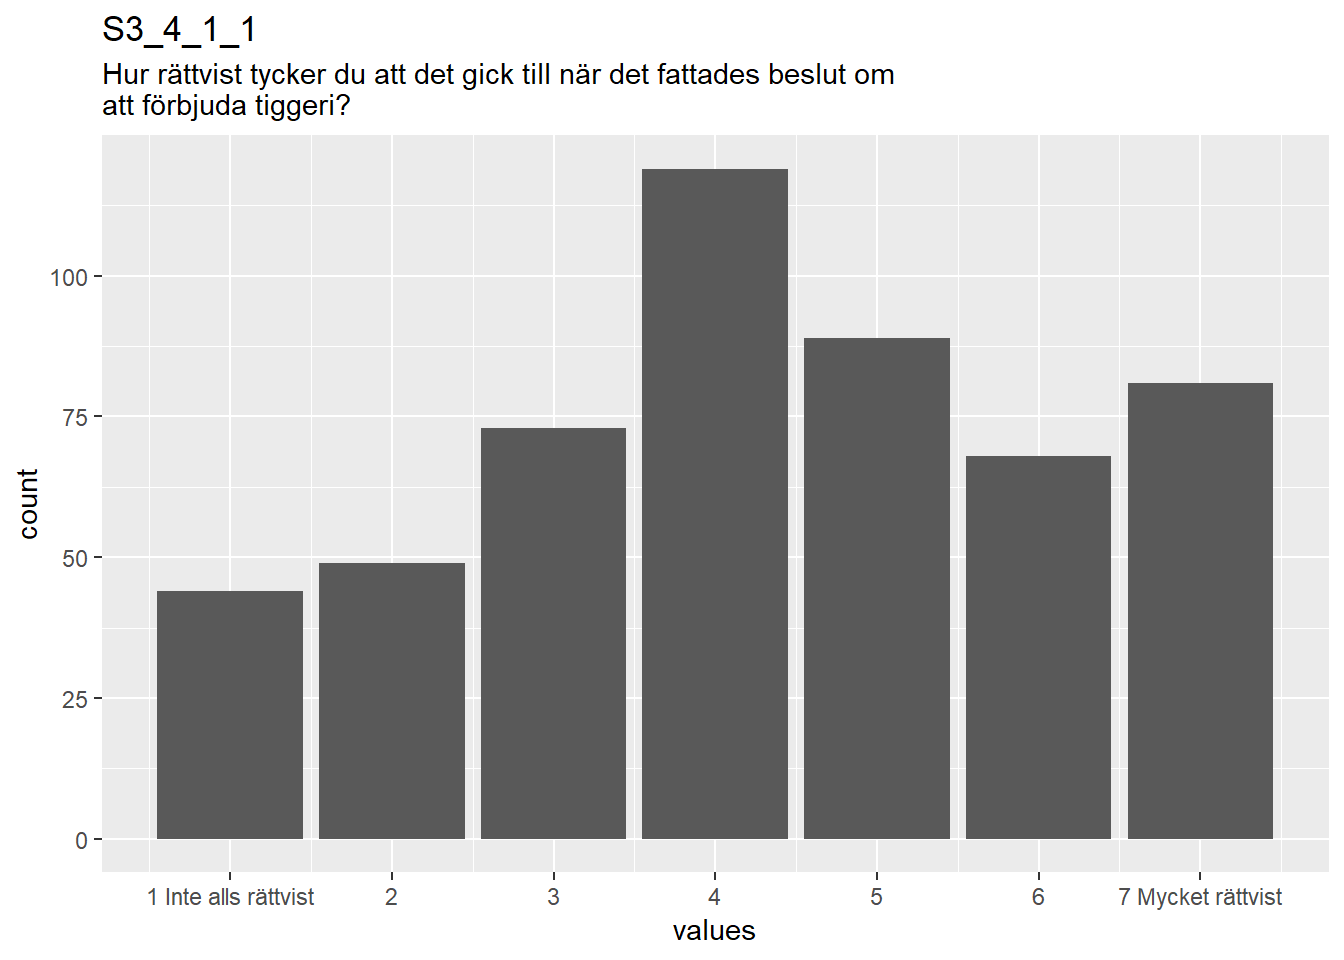
\includegraphics{Goodloser-appendix_files/figure-latex/S3_4_1_1_distribution-1.pdf}

\begin{Shaded}
\begin{Highlighting}[]
\NormalTok{knitr}\OperatorTok{::}\NormalTok{opts_chunk}\OperatorTok{$}\KeywordTok{set}\NormalTok{(}\DataTypeTok{fig.height =}\NormalTok{ old_height)}
\end{Highlighting}
\end{Shaded}

496 missings.

\subsubsection{Summary statistics}\label{S3_4_1_1_summary}

\begin{Shaded}
\begin{Highlighting}[]
\KeywordTok{attributes}\NormalTok{(item) <-}\StringTok{ }\NormalTok{item_attributes}
\NormalTok{df =}\StringTok{ }\KeywordTok{data.frame}\NormalTok{(item, }\DataTypeTok{stringsAsFactors =} \OtherTok{FALSE}\NormalTok{)}
\KeywordTok{names}\NormalTok{(df) =}\StringTok{ }\NormalTok{html_item_name}
\KeywordTok{escaped_table}\NormalTok{(}\KeywordTok{codebook_table}\NormalTok{(df))}
\end{Highlighting}
\end{Shaded}

name

label

data\_type

value\_labels

missing

complete

n

mean

sd

p0

p25

p50

p75

p100

hist

format.spss

display\_width

S3\_4\_1\_1

Hur rättvist tycker du att det gick till när det fattades beslut om att
förbjuda tiggeri?

numeric

\begin{enumerate}
\def\labelenumi{\arabic{enumi}.}
\tightlist
\item
  1 Inte alls rättvist,2. 2,3. 3,4. 4,5. 5,6. 6,7. 7 Mycket rättvist

  496

  523

  1019

  4.32

  1.81

  1

  3

  4

  6

  7

  ▃▃▅▇▁▆▅▆

  F1.0

  12
\end{enumerate}

\begin{Shaded}
\begin{Highlighting}[]
\ControlFlowTok{if}\NormalTok{ (show_missings) \{}
  \KeywordTok{plot_labelled}\NormalTok{(missings, item_name, wrap_at)}
\NormalTok{\}}
\end{Highlighting}
\end{Shaded}

\begin{Shaded}
\begin{Highlighting}[]
\ControlFlowTok{if}\NormalTok{ (}\OperatorTok{!}\KeywordTok{is.null}\NormalTok{(item_info)) \{}
  \CommentTok{# don't show choices again, if they're basically same thing as value labels}
  \ControlFlowTok{if}\NormalTok{ (}\OperatorTok{!}\KeywordTok{is.null}\NormalTok{(choices) }\OperatorTok{&&}\StringTok{ }\OperatorTok{!}\KeywordTok{is.null}\NormalTok{(item_info}\OperatorTok{$}\NormalTok{choices) }\OperatorTok{&&}\StringTok{ }
\StringTok{    }\KeywordTok{all}\NormalTok{(}\KeywordTok{names}\NormalTok{(}\KeywordTok{na.omit}\NormalTok{(choices)) }\OperatorTok{==}\StringTok{ }\NormalTok{item_info}\OperatorTok{$}\NormalTok{choices) }\OperatorTok{&&}
\StringTok{    }\KeywordTok{all}\NormalTok{(}\KeywordTok{na.omit}\NormalTok{(choices) }\OperatorTok{==}\StringTok{ }\KeywordTok{names}\NormalTok{(item_info}\OperatorTok{$}\NormalTok{choices))) \{}
\NormalTok{    item_info}\OperatorTok{$}\NormalTok{choices <-}\StringTok{ }\OtherTok{NULL}
\NormalTok{  \}}
\NormalTok{  item_info}\OperatorTok{$}\NormalTok{label_parsed <-}\StringTok{ }
\StringTok{    }\NormalTok{item_info}\OperatorTok{$}\NormalTok{choice_list <-}\StringTok{ }\NormalTok{item_info}\OperatorTok{$}\NormalTok{study_id <-}\StringTok{ }\NormalTok{item_info}\OperatorTok{$}\NormalTok{id <-}\StringTok{ }\OtherTok{NULL}
\NormalTok{  pander}\OperatorTok{::}\KeywordTok{pander}\NormalTok{(item_info)}
\NormalTok{\}}
\end{Highlighting}
\end{Shaded}

\subsubsection{Value labels}\label{S3_4_1_1_labels}

\begin{Shaded}
\begin{Highlighting}[]
\ControlFlowTok{if}\NormalTok{ (}\OperatorTok{!}\KeywordTok{is.null}\NormalTok{(choices) }\OperatorTok{&&}\StringTok{ }\KeywordTok{length}\NormalTok{(choices) }\OperatorTok{&&}\StringTok{ }\KeywordTok{length}\NormalTok{(choices) }\OperatorTok{<}\StringTok{ }\DecValTok{30}\NormalTok{) \{}
\NormalTok{    pander}\OperatorTok{::}\KeywordTok{pander}\NormalTok{(}\KeywordTok{as.list}\NormalTok{(choices))}
\NormalTok{\}}
\end{Highlighting}
\end{Shaded}

\begin{itemize}
\tightlist
\item
  \textbf{1 Inte alls rättvist}: \emph{1}
\item
  \textbf{2}: \emph{2}
\item
  \textbf{3}: \emph{3}
\item
  \textbf{4}: \emph{4}
\item
  \textbf{5}: \emph{5}
\item
  \textbf{6}: \emph{6}
\item
  \textbf{7 Mycket rättvist}: \emph{7}
\end{itemize}

\subsection{S3\_4\_1\_2}\label{S3_4_1_2}

Hur rättvist tycker du att det gick till när det fattades beslut om att
inte förbjuda tiggeri?

\subsubsection{Distribution}\label{S3_4_1_2_distribution}

\begin{Shaded}
\begin{Highlighting}[]
\NormalTok{show_missings <-}\StringTok{ }\OtherTok{FALSE}
\ControlFlowTok{if}\NormalTok{ (}\KeywordTok{has_label}\NormalTok{(item)) \{}
\NormalTok{  missings <-}\StringTok{ }\NormalTok{item[}\KeywordTok{is.na}\NormalTok{(haven}\OperatorTok{::}\KeywordTok{zap_missing}\NormalTok{(item))]}
  \KeywordTok{attributes}\NormalTok{(missings) <-}\StringTok{ }\KeywordTok{attributes}\NormalTok{(item)}
  \ControlFlowTok{if}\NormalTok{ (}\OperatorTok{!}\KeywordTok{is.null}\NormalTok{(}\KeywordTok{attributes}\NormalTok{(item)}\OperatorTok{$}\NormalTok{labels)) \{}
    \KeywordTok{attributes}\NormalTok{(missings)}\OperatorTok{$}\NormalTok{labels <-}\StringTok{ }\KeywordTok{attributes}\NormalTok{(missings)}\OperatorTok{$}\NormalTok{labels[}\KeywordTok{is.na}\NormalTok{(}\KeywordTok{attributes}\NormalTok{(missings)}\OperatorTok{$}\NormalTok{labels)]}
    \KeywordTok{attributes}\NormalTok{(item)}\OperatorTok{$}\NormalTok{labels <-}\StringTok{ }\KeywordTok{attributes}\NormalTok{(item)}\OperatorTok{$}\NormalTok{labels[}\OperatorTok{!}\KeywordTok{is.na}\NormalTok{(}\KeywordTok{attributes}\NormalTok{(item)}\OperatorTok{$}\NormalTok{labels)]}
\NormalTok{  \}}
  \ControlFlowTok{if}\NormalTok{ (}\KeywordTok{is.numeric}\NormalTok{(item)) \{}
\NormalTok{    show_missings <-}\StringTok{ }\KeywordTok{length}\NormalTok{(}\KeywordTok{unique}\NormalTok{(haven}\OperatorTok{::}\KeywordTok{na_tag}\NormalTok{(missings))) }\OperatorTok{>}\StringTok{ }\DecValTok{1}
\NormalTok{    item <-}\StringTok{ }\NormalTok{haven}\OperatorTok{::}\KeywordTok{zap_missing}\NormalTok{(item)}
\NormalTok{  \}}
  \ControlFlowTok{if}\NormalTok{ (}\KeywordTok{length}\NormalTok{(item_attributes}\OperatorTok{$}\NormalTok{labels) }\OperatorTok{==}\StringTok{ }\DecValTok{0} \OperatorTok{&&}\StringTok{ }\KeywordTok{is.numeric}\NormalTok{(item)) \{}
\NormalTok{    item <-}\StringTok{ }\NormalTok{haven}\OperatorTok{::}\KeywordTok{zap_labels}\NormalTok{(item)}
\NormalTok{  \}}
\NormalTok{\}}
\NormalTok{item_nomiss <-}\StringTok{ }\NormalTok{item[}\OperatorTok{!}\KeywordTok{is.na}\NormalTok{(item)]}

\CommentTok{# unnest mc_multiple and so on}
\ControlFlowTok{if}\NormalTok{ (}
  \KeywordTok{is.character}\NormalTok{(item_nomiss) }\OperatorTok{&&}
\StringTok{  }\NormalTok{stringr}\OperatorTok{::}\KeywordTok{str_detect}\NormalTok{(item_nomiss, stringr}\OperatorTok{::}\KeywordTok{fixed}\NormalTok{(}\StringTok{", "}\NormalTok{)) }\OperatorTok{&&}
\StringTok{  }\NormalTok{(}\KeywordTok{exists}\NormalTok{(}\StringTok{"type"}\NormalTok{, item_info) }\OperatorTok{&&}\StringTok{ }
\StringTok{    }\NormalTok{stringr}\OperatorTok{::}\KeywordTok{str_detect}\NormalTok{(item_info}\OperatorTok{$}\NormalTok{type, }\DataTypeTok{pattern =}\NormalTok{ stringr}\OperatorTok{::}\KeywordTok{fixed}\NormalTok{(}\StringTok{"multiple"}\NormalTok{)))}
\NormalTok{  ) \{}
\NormalTok{  item_nomiss <-}\StringTok{ }\KeywordTok{unlist}\NormalTok{(stringr}\OperatorTok{::}\KeywordTok{str_split}\NormalTok{(item_nomiss, }\DataTypeTok{pattern =}\NormalTok{ stringr}\OperatorTok{::}\KeywordTok{fixed}\NormalTok{(}\StringTok{", "}\NormalTok{)))}
\NormalTok{\}}
\KeywordTok{attributes}\NormalTok{(item_nomiss) <-}\StringTok{ }\KeywordTok{attributes}\NormalTok{(item)}

\NormalTok{old_height <-}\StringTok{ }\NormalTok{knitr}\OperatorTok{::}\NormalTok{opts_chunk}\OperatorTok{$}\KeywordTok{get}\NormalTok{(}\StringTok{"fig.height"}\NormalTok{)}
\NormalTok{non_missing_choices <-}\StringTok{ }\NormalTok{item_attributes[[}\StringTok{"labels"}\NormalTok{]]}
\NormalTok{many_labels <-}\StringTok{ }\KeywordTok{length}\NormalTok{(non_missing_choices) }\OperatorTok{>}\StringTok{ }\DecValTok{7}
\NormalTok{go_vertical <-}\StringTok{ }\OperatorTok{!}\KeywordTok{is.numeric}\NormalTok{(item_nomiss) }\OperatorTok{||}\StringTok{ }\NormalTok{many_labels}
\ControlFlowTok{if}\NormalTok{ ( go_vertical ) \{}
  \CommentTok{# numeric items are plotted horizontally (because that's what usually expected)}
  \CommentTok{# categorical items are plotted vertically because we can use the screen real estate better this way}

    \ControlFlowTok{if}\NormalTok{ (}\KeywordTok{is.null}\NormalTok{(choices) }\OperatorTok{||}\StringTok{ }
\StringTok{        }\NormalTok{dplyr}\OperatorTok{::}\KeywordTok{n_distinct}\NormalTok{(item_nomiss) }\OperatorTok{>}\StringTok{ }\KeywordTok{length}\NormalTok{(non_missing_choices)) \{}
\NormalTok{        non_missing_choices <-}\StringTok{ }\KeywordTok{unique}\NormalTok{(item_nomiss)}
        \KeywordTok{names}\NormalTok{(non_missing_choices) <-}\StringTok{ }\NormalTok{non_missing_choices}
\NormalTok{    \}}
\NormalTok{  choice_multiplier <-}\StringTok{ }\NormalTok{old_height}\OperatorTok{/}\FloatTok{6.5}
\NormalTok{    new_height <-}\StringTok{ }\DecValTok{2} \OperatorTok{+}\StringTok{ }\NormalTok{choice_multiplier }\OperatorTok{*}\StringTok{ }\KeywordTok{length}\NormalTok{(non_missing_choices)}
\NormalTok{    new_height <-}\StringTok{ }\KeywordTok{ifelse}\NormalTok{(new_height }\OperatorTok{>}\StringTok{ }\DecValTok{20}\NormalTok{, }\DecValTok{20}\NormalTok{, new_height)}
\NormalTok{    new_height <-}\StringTok{ }\KeywordTok{ifelse}\NormalTok{(new_height }\OperatorTok{<}\StringTok{ }\DecValTok{1}\NormalTok{, }\DecValTok{1}\NormalTok{, new_height)}
\NormalTok{    knitr}\OperatorTok{::}\NormalTok{opts_chunk}\OperatorTok{$}\KeywordTok{set}\NormalTok{(}\DataTypeTok{fig.height =}\NormalTok{ new_height)}
\NormalTok{\}}

\NormalTok{wrap_at <-}\StringTok{ }\NormalTok{knitr}\OperatorTok{::}\NormalTok{opts_chunk}\OperatorTok{$}\KeywordTok{get}\NormalTok{(}\StringTok{"fig.width"}\NormalTok{) }\OperatorTok{*}\StringTok{ }\DecValTok{10}
\end{Highlighting}
\end{Shaded}

\begin{Shaded}
\begin{Highlighting}[]
\CommentTok{# todo: if there are free-text choices mingled in with the pre-defined ones, don't show}
\CommentTok{# todo: show rare items if they are pre-defined}
\CommentTok{# todo: bin rare responses into "other category"}
\ControlFlowTok{if}\NormalTok{ (}\OperatorTok{!}\KeywordTok{length}\NormalTok{(item_nomiss)) \{}
  \KeywordTok{cat}\NormalTok{(}\StringTok{"No non-missing values to show."}\NormalTok{)}
\NormalTok{\} }\ControlFlowTok{else} \ControlFlowTok{if}\NormalTok{ (}\KeywordTok{is.numeric}\NormalTok{(item_nomiss) }\OperatorTok{||}\StringTok{ }\NormalTok{dplyr}\OperatorTok{::}\KeywordTok{n_distinct}\NormalTok{(item_nomiss) }\OperatorTok{<}\StringTok{ }\DecValTok{20}\NormalTok{) \{}
  \KeywordTok{plot_labelled}\NormalTok{(item_nomiss, item_name, wrap_at, go_vertical)}
\NormalTok{\} }\ControlFlowTok{else}\NormalTok{ \{}
    \KeywordTok{cat}\NormalTok{(dplyr}\OperatorTok{::}\KeywordTok{n_distinct}\NormalTok{(item_nomiss), }\StringTok{" unique, categorical values, so not shown."}\NormalTok{)}
\NormalTok{\}}
\end{Highlighting}
\end{Shaded}

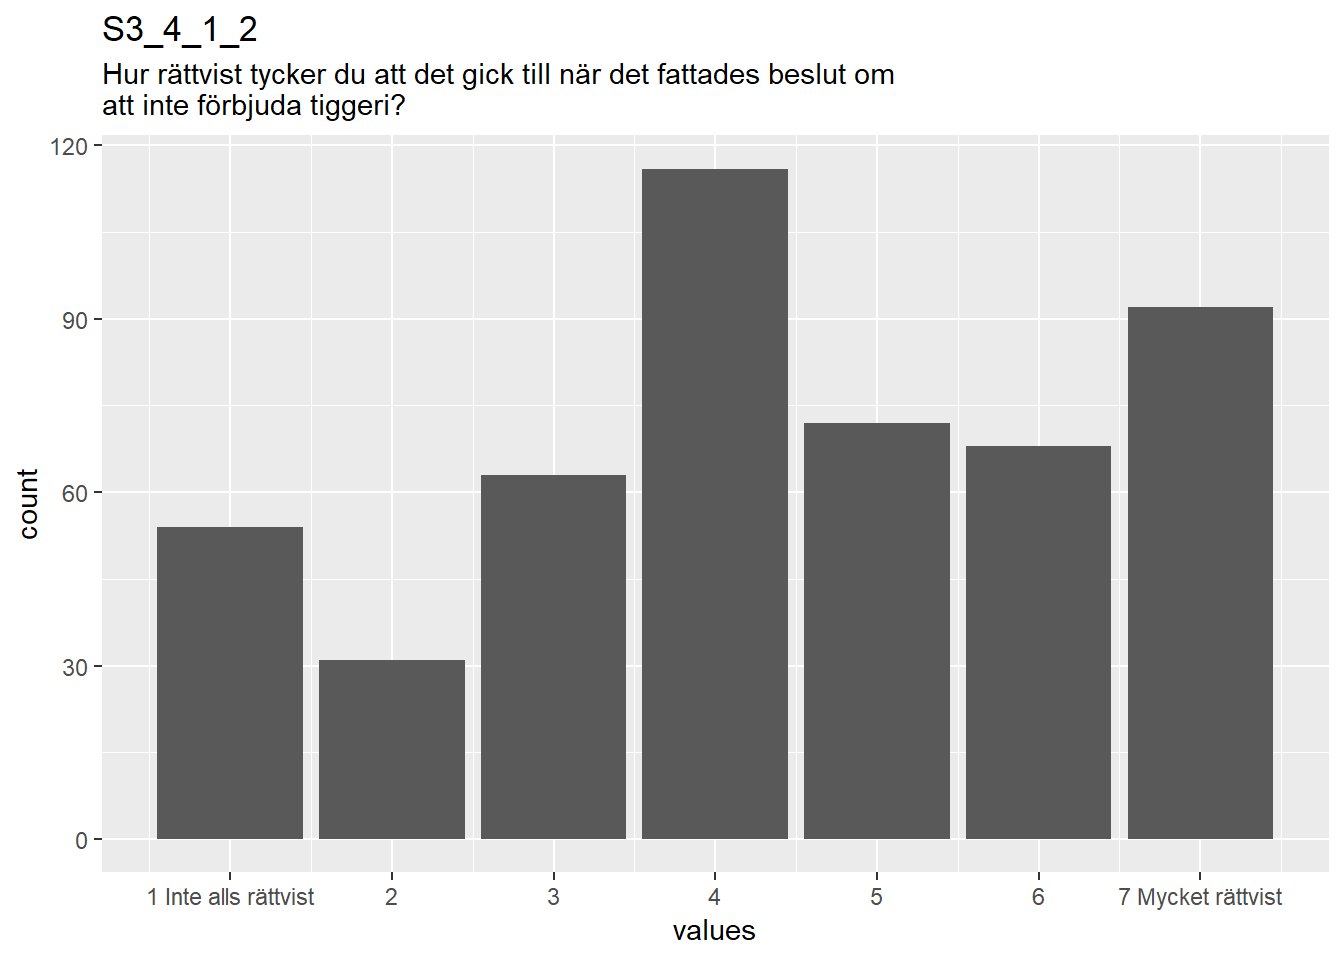
\includegraphics{Goodloser-appendix_files/figure-latex/S3_4_1_2_distribution-1.pdf}

\begin{Shaded}
\begin{Highlighting}[]
\NormalTok{knitr}\OperatorTok{::}\NormalTok{opts_chunk}\OperatorTok{$}\KeywordTok{set}\NormalTok{(}\DataTypeTok{fig.height =}\NormalTok{ old_height)}
\end{Highlighting}
\end{Shaded}

523 missings.

\subsubsection{Summary statistics}\label{S3_4_1_2_summary}

\begin{Shaded}
\begin{Highlighting}[]
\KeywordTok{attributes}\NormalTok{(item) <-}\StringTok{ }\NormalTok{item_attributes}
\NormalTok{df =}\StringTok{ }\KeywordTok{data.frame}\NormalTok{(item, }\DataTypeTok{stringsAsFactors =} \OtherTok{FALSE}\NormalTok{)}
\KeywordTok{names}\NormalTok{(df) =}\StringTok{ }\NormalTok{html_item_name}
\KeywordTok{escaped_table}\NormalTok{(}\KeywordTok{codebook_table}\NormalTok{(df))}
\end{Highlighting}
\end{Shaded}

name

label

data\_type

value\_labels

missing

complete

n

mean

sd

p0

p25

p50

p75

p100

hist

format.spss

S3\_4\_1\_2

Hur rättvist tycker du att det gick till när det fattades beslut om att
inte förbjuda tiggeri?

numeric

\begin{enumerate}
\def\labelenumi{\arabic{enumi}.}
\tightlist
\item
  1 Inte alls rättvist,2. 2,3. 3,4. 4,5. 5,6. 6,7. 7 Mycket rättvist

  523

  496

  1019

  4.4

  1.89

  1

  3

  4

  6

  7

  ▃▂▅▇▁▅▅▆

  F1.0
\end{enumerate}

\begin{Shaded}
\begin{Highlighting}[]
\ControlFlowTok{if}\NormalTok{ (show_missings) \{}
  \KeywordTok{plot_labelled}\NormalTok{(missings, item_name, wrap_at)}
\NormalTok{\}}
\end{Highlighting}
\end{Shaded}

\begin{Shaded}
\begin{Highlighting}[]
\ControlFlowTok{if}\NormalTok{ (}\OperatorTok{!}\KeywordTok{is.null}\NormalTok{(item_info)) \{}
  \CommentTok{# don't show choices again, if they're basically same thing as value labels}
  \ControlFlowTok{if}\NormalTok{ (}\OperatorTok{!}\KeywordTok{is.null}\NormalTok{(choices) }\OperatorTok{&&}\StringTok{ }\OperatorTok{!}\KeywordTok{is.null}\NormalTok{(item_info}\OperatorTok{$}\NormalTok{choices) }\OperatorTok{&&}\StringTok{ }
\StringTok{    }\KeywordTok{all}\NormalTok{(}\KeywordTok{names}\NormalTok{(}\KeywordTok{na.omit}\NormalTok{(choices)) }\OperatorTok{==}\StringTok{ }\NormalTok{item_info}\OperatorTok{$}\NormalTok{choices) }\OperatorTok{&&}
\StringTok{    }\KeywordTok{all}\NormalTok{(}\KeywordTok{na.omit}\NormalTok{(choices) }\OperatorTok{==}\StringTok{ }\KeywordTok{names}\NormalTok{(item_info}\OperatorTok{$}\NormalTok{choices))) \{}
\NormalTok{    item_info}\OperatorTok{$}\NormalTok{choices <-}\StringTok{ }\OtherTok{NULL}
\NormalTok{  \}}
\NormalTok{  item_info}\OperatorTok{$}\NormalTok{label_parsed <-}\StringTok{ }
\StringTok{    }\NormalTok{item_info}\OperatorTok{$}\NormalTok{choice_list <-}\StringTok{ }\NormalTok{item_info}\OperatorTok{$}\NormalTok{study_id <-}\StringTok{ }\NormalTok{item_info}\OperatorTok{$}\NormalTok{id <-}\StringTok{ }\OtherTok{NULL}
\NormalTok{  pander}\OperatorTok{::}\KeywordTok{pander}\NormalTok{(item_info)}
\NormalTok{\}}
\end{Highlighting}
\end{Shaded}

\subsubsection{Value labels}\label{S3_4_1_2_labels}

\begin{Shaded}
\begin{Highlighting}[]
\ControlFlowTok{if}\NormalTok{ (}\OperatorTok{!}\KeywordTok{is.null}\NormalTok{(choices) }\OperatorTok{&&}\StringTok{ }\KeywordTok{length}\NormalTok{(choices) }\OperatorTok{&&}\StringTok{ }\KeywordTok{length}\NormalTok{(choices) }\OperatorTok{<}\StringTok{ }\DecValTok{30}\NormalTok{) \{}
\NormalTok{    pander}\OperatorTok{::}\KeywordTok{pander}\NormalTok{(}\KeywordTok{as.list}\NormalTok{(choices))}
\NormalTok{\}}
\end{Highlighting}
\end{Shaded}

\begin{itemize}
\tightlist
\item
  \textbf{1 Inte alls rättvist}: \emph{1}
\item
  \textbf{2}: \emph{2}
\item
  \textbf{3}: \emph{3}
\item
  \textbf{4}: \emph{4}
\item
  \textbf{5}: \emph{5}
\item
  \textbf{6}: \emph{6}
\item
  \textbf{7 Mycket rättvist}: \emph{7}
\end{itemize}

\subsection{S3\_5\_1}\label{S3_5_1}

Och hur schysst tycker du att beslutsproceduren var?

\subsubsection{Distribution}\label{S3_5_1_distribution}

\begin{Shaded}
\begin{Highlighting}[]
\NormalTok{show_missings <-}\StringTok{ }\OtherTok{FALSE}
\ControlFlowTok{if}\NormalTok{ (}\KeywordTok{has_label}\NormalTok{(item)) \{}
\NormalTok{  missings <-}\StringTok{ }\NormalTok{item[}\KeywordTok{is.na}\NormalTok{(haven}\OperatorTok{::}\KeywordTok{zap_missing}\NormalTok{(item))]}
  \KeywordTok{attributes}\NormalTok{(missings) <-}\StringTok{ }\KeywordTok{attributes}\NormalTok{(item)}
  \ControlFlowTok{if}\NormalTok{ (}\OperatorTok{!}\KeywordTok{is.null}\NormalTok{(}\KeywordTok{attributes}\NormalTok{(item)}\OperatorTok{$}\NormalTok{labels)) \{}
    \KeywordTok{attributes}\NormalTok{(missings)}\OperatorTok{$}\NormalTok{labels <-}\StringTok{ }\KeywordTok{attributes}\NormalTok{(missings)}\OperatorTok{$}\NormalTok{labels[}\KeywordTok{is.na}\NormalTok{(}\KeywordTok{attributes}\NormalTok{(missings)}\OperatorTok{$}\NormalTok{labels)]}
    \KeywordTok{attributes}\NormalTok{(item)}\OperatorTok{$}\NormalTok{labels <-}\StringTok{ }\KeywordTok{attributes}\NormalTok{(item)}\OperatorTok{$}\NormalTok{labels[}\OperatorTok{!}\KeywordTok{is.na}\NormalTok{(}\KeywordTok{attributes}\NormalTok{(item)}\OperatorTok{$}\NormalTok{labels)]}
\NormalTok{  \}}
  \ControlFlowTok{if}\NormalTok{ (}\KeywordTok{is.numeric}\NormalTok{(item)) \{}
\NormalTok{    show_missings <-}\StringTok{ }\KeywordTok{length}\NormalTok{(}\KeywordTok{unique}\NormalTok{(haven}\OperatorTok{::}\KeywordTok{na_tag}\NormalTok{(missings))) }\OperatorTok{>}\StringTok{ }\DecValTok{1}
\NormalTok{    item <-}\StringTok{ }\NormalTok{haven}\OperatorTok{::}\KeywordTok{zap_missing}\NormalTok{(item)}
\NormalTok{  \}}
  \ControlFlowTok{if}\NormalTok{ (}\KeywordTok{length}\NormalTok{(item_attributes}\OperatorTok{$}\NormalTok{labels) }\OperatorTok{==}\StringTok{ }\DecValTok{0} \OperatorTok{&&}\StringTok{ }\KeywordTok{is.numeric}\NormalTok{(item)) \{}
\NormalTok{    item <-}\StringTok{ }\NormalTok{haven}\OperatorTok{::}\KeywordTok{zap_labels}\NormalTok{(item)}
\NormalTok{  \}}
\NormalTok{\}}
\NormalTok{item_nomiss <-}\StringTok{ }\NormalTok{item[}\OperatorTok{!}\KeywordTok{is.na}\NormalTok{(item)]}

\CommentTok{# unnest mc_multiple and so on}
\ControlFlowTok{if}\NormalTok{ (}
  \KeywordTok{is.character}\NormalTok{(item_nomiss) }\OperatorTok{&&}
\StringTok{  }\NormalTok{stringr}\OperatorTok{::}\KeywordTok{str_detect}\NormalTok{(item_nomiss, stringr}\OperatorTok{::}\KeywordTok{fixed}\NormalTok{(}\StringTok{", "}\NormalTok{)) }\OperatorTok{&&}
\StringTok{  }\NormalTok{(}\KeywordTok{exists}\NormalTok{(}\StringTok{"type"}\NormalTok{, item_info) }\OperatorTok{&&}\StringTok{ }
\StringTok{    }\NormalTok{stringr}\OperatorTok{::}\KeywordTok{str_detect}\NormalTok{(item_info}\OperatorTok{$}\NormalTok{type, }\DataTypeTok{pattern =}\NormalTok{ stringr}\OperatorTok{::}\KeywordTok{fixed}\NormalTok{(}\StringTok{"multiple"}\NormalTok{)))}
\NormalTok{  ) \{}
\NormalTok{  item_nomiss <-}\StringTok{ }\KeywordTok{unlist}\NormalTok{(stringr}\OperatorTok{::}\KeywordTok{str_split}\NormalTok{(item_nomiss, }\DataTypeTok{pattern =}\NormalTok{ stringr}\OperatorTok{::}\KeywordTok{fixed}\NormalTok{(}\StringTok{", "}\NormalTok{)))}
\NormalTok{\}}
\KeywordTok{attributes}\NormalTok{(item_nomiss) <-}\StringTok{ }\KeywordTok{attributes}\NormalTok{(item)}

\NormalTok{old_height <-}\StringTok{ }\NormalTok{knitr}\OperatorTok{::}\NormalTok{opts_chunk}\OperatorTok{$}\KeywordTok{get}\NormalTok{(}\StringTok{"fig.height"}\NormalTok{)}
\NormalTok{non_missing_choices <-}\StringTok{ }\NormalTok{item_attributes[[}\StringTok{"labels"}\NormalTok{]]}
\NormalTok{many_labels <-}\StringTok{ }\KeywordTok{length}\NormalTok{(non_missing_choices) }\OperatorTok{>}\StringTok{ }\DecValTok{7}
\NormalTok{go_vertical <-}\StringTok{ }\OperatorTok{!}\KeywordTok{is.numeric}\NormalTok{(item_nomiss) }\OperatorTok{||}\StringTok{ }\NormalTok{many_labels}
\ControlFlowTok{if}\NormalTok{ ( go_vertical ) \{}
  \CommentTok{# numeric items are plotted horizontally (because that's what usually expected)}
  \CommentTok{# categorical items are plotted vertically because we can use the screen real estate better this way}

    \ControlFlowTok{if}\NormalTok{ (}\KeywordTok{is.null}\NormalTok{(choices) }\OperatorTok{||}\StringTok{ }
\StringTok{        }\NormalTok{dplyr}\OperatorTok{::}\KeywordTok{n_distinct}\NormalTok{(item_nomiss) }\OperatorTok{>}\StringTok{ }\KeywordTok{length}\NormalTok{(non_missing_choices)) \{}
\NormalTok{        non_missing_choices <-}\StringTok{ }\KeywordTok{unique}\NormalTok{(item_nomiss)}
        \KeywordTok{names}\NormalTok{(non_missing_choices) <-}\StringTok{ }\NormalTok{non_missing_choices}
\NormalTok{    \}}
\NormalTok{  choice_multiplier <-}\StringTok{ }\NormalTok{old_height}\OperatorTok{/}\FloatTok{6.5}
\NormalTok{    new_height <-}\StringTok{ }\DecValTok{2} \OperatorTok{+}\StringTok{ }\NormalTok{choice_multiplier }\OperatorTok{*}\StringTok{ }\KeywordTok{length}\NormalTok{(non_missing_choices)}
\NormalTok{    new_height <-}\StringTok{ }\KeywordTok{ifelse}\NormalTok{(new_height }\OperatorTok{>}\StringTok{ }\DecValTok{20}\NormalTok{, }\DecValTok{20}\NormalTok{, new_height)}
\NormalTok{    new_height <-}\StringTok{ }\KeywordTok{ifelse}\NormalTok{(new_height }\OperatorTok{<}\StringTok{ }\DecValTok{1}\NormalTok{, }\DecValTok{1}\NormalTok{, new_height)}
\NormalTok{    knitr}\OperatorTok{::}\NormalTok{opts_chunk}\OperatorTok{$}\KeywordTok{set}\NormalTok{(}\DataTypeTok{fig.height =}\NormalTok{ new_height)}
\NormalTok{\}}

\NormalTok{wrap_at <-}\StringTok{ }\NormalTok{knitr}\OperatorTok{::}\NormalTok{opts_chunk}\OperatorTok{$}\KeywordTok{get}\NormalTok{(}\StringTok{"fig.width"}\NormalTok{) }\OperatorTok{*}\StringTok{ }\DecValTok{10}
\end{Highlighting}
\end{Shaded}

\begin{Shaded}
\begin{Highlighting}[]
\CommentTok{# todo: if there are free-text choices mingled in with the pre-defined ones, don't show}
\CommentTok{# todo: show rare items if they are pre-defined}
\CommentTok{# todo: bin rare responses into "other category"}
\ControlFlowTok{if}\NormalTok{ (}\OperatorTok{!}\KeywordTok{length}\NormalTok{(item_nomiss)) \{}
  \KeywordTok{cat}\NormalTok{(}\StringTok{"No non-missing values to show."}\NormalTok{)}
\NormalTok{\} }\ControlFlowTok{else} \ControlFlowTok{if}\NormalTok{ (}\KeywordTok{is.numeric}\NormalTok{(item_nomiss) }\OperatorTok{||}\StringTok{ }\NormalTok{dplyr}\OperatorTok{::}\KeywordTok{n_distinct}\NormalTok{(item_nomiss) }\OperatorTok{<}\StringTok{ }\DecValTok{20}\NormalTok{) \{}
  \KeywordTok{plot_labelled}\NormalTok{(item_nomiss, item_name, wrap_at, go_vertical)}
\NormalTok{\} }\ControlFlowTok{else}\NormalTok{ \{}
    \KeywordTok{cat}\NormalTok{(dplyr}\OperatorTok{::}\KeywordTok{n_distinct}\NormalTok{(item_nomiss), }\StringTok{" unique, categorical values, so not shown."}\NormalTok{)}
\NormalTok{\}}
\end{Highlighting}
\end{Shaded}

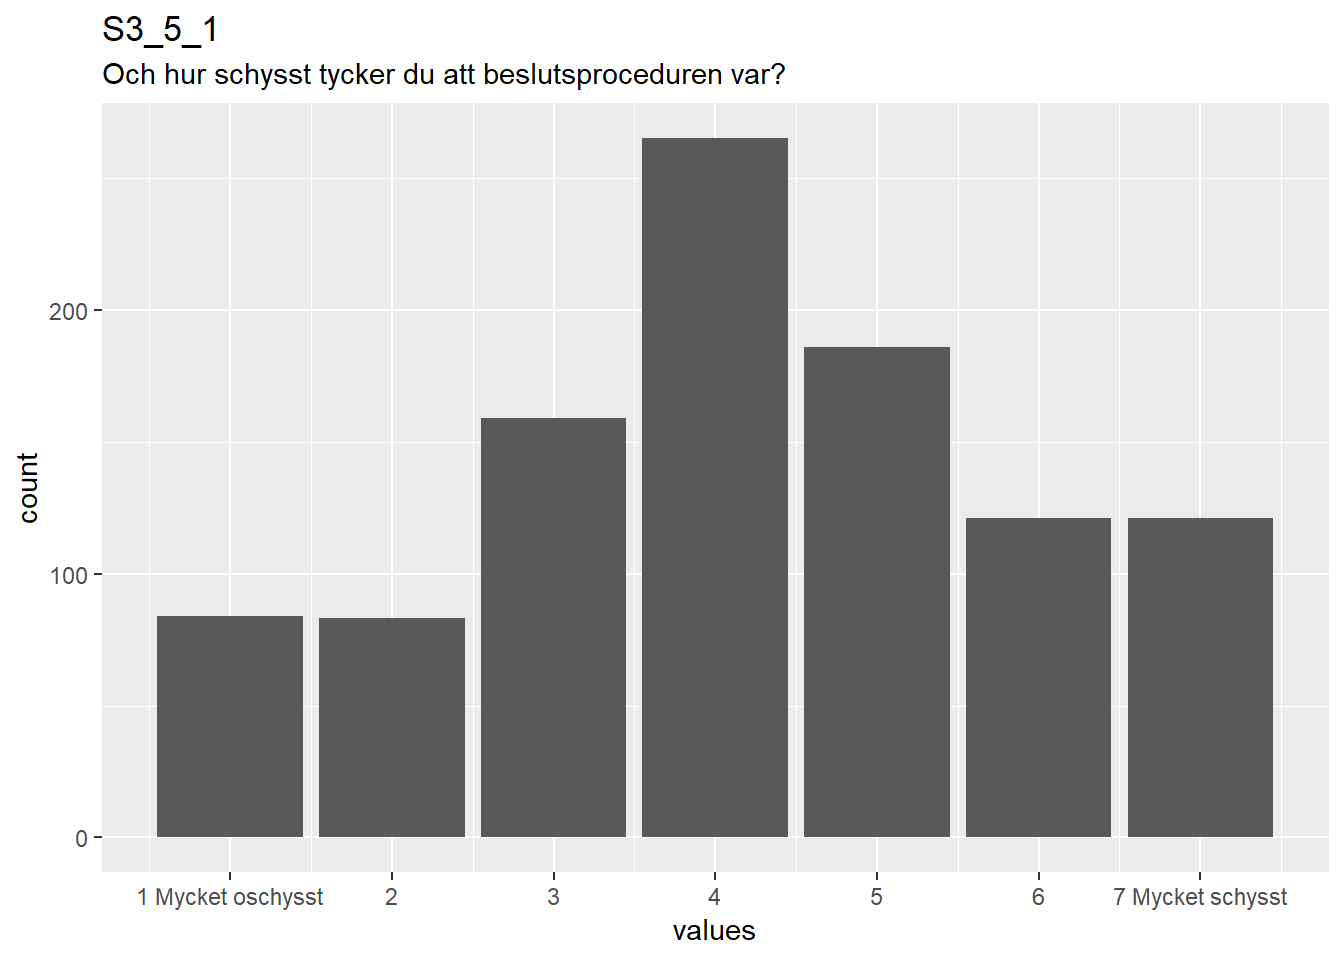
\includegraphics{Goodloser-appendix_files/figure-latex/S3_5_1_distribution-1.pdf}

\begin{Shaded}
\begin{Highlighting}[]
\NormalTok{knitr}\OperatorTok{::}\NormalTok{opts_chunk}\OperatorTok{$}\KeywordTok{set}\NormalTok{(}\DataTypeTok{fig.height =}\NormalTok{ old_height)}
\end{Highlighting}
\end{Shaded}

0 missings.

\subsubsection{Summary statistics}\label{S3_5_1_summary}

\begin{Shaded}
\begin{Highlighting}[]
\KeywordTok{attributes}\NormalTok{(item) <-}\StringTok{ }\NormalTok{item_attributes}
\NormalTok{df =}\StringTok{ }\KeywordTok{data.frame}\NormalTok{(item, }\DataTypeTok{stringsAsFactors =} \OtherTok{FALSE}\NormalTok{)}
\KeywordTok{names}\NormalTok{(df) =}\StringTok{ }\NormalTok{html_item_name}
\KeywordTok{escaped_table}\NormalTok{(}\KeywordTok{codebook_table}\NormalTok{(df))}
\end{Highlighting}
\end{Shaded}

name

label

data\_type

value\_labels

missing

complete

n

mean

sd

p0

p25

p50

p75

p100

hist

format.spss

display\_width

S3\_5\_1

Och hur schysst tycker du att beslutsproceduren var?

numeric

\begin{enumerate}
\def\labelenumi{\arabic{enumi}.}
\tightlist
\item
  1 Mycket oschysst,2. 2,3. 3,4. 4,5. 5,6. 6,7. 7 Mycket schysst

  0

  1019

  1019

  4.21

  1.71

  1

  3

  4

  5

  7

  ▂▂▅▇▁▆▃▃

  F1.0

  12
\end{enumerate}

\begin{Shaded}
\begin{Highlighting}[]
\ControlFlowTok{if}\NormalTok{ (show_missings) \{}
  \KeywordTok{plot_labelled}\NormalTok{(missings, item_name, wrap_at)}
\NormalTok{\}}
\end{Highlighting}
\end{Shaded}

\begin{Shaded}
\begin{Highlighting}[]
\ControlFlowTok{if}\NormalTok{ (}\OperatorTok{!}\KeywordTok{is.null}\NormalTok{(item_info)) \{}
  \CommentTok{# don't show choices again, if they're basically same thing as value labels}
  \ControlFlowTok{if}\NormalTok{ (}\OperatorTok{!}\KeywordTok{is.null}\NormalTok{(choices) }\OperatorTok{&&}\StringTok{ }\OperatorTok{!}\KeywordTok{is.null}\NormalTok{(item_info}\OperatorTok{$}\NormalTok{choices) }\OperatorTok{&&}\StringTok{ }
\StringTok{    }\KeywordTok{all}\NormalTok{(}\KeywordTok{names}\NormalTok{(}\KeywordTok{na.omit}\NormalTok{(choices)) }\OperatorTok{==}\StringTok{ }\NormalTok{item_info}\OperatorTok{$}\NormalTok{choices) }\OperatorTok{&&}
\StringTok{    }\KeywordTok{all}\NormalTok{(}\KeywordTok{na.omit}\NormalTok{(choices) }\OperatorTok{==}\StringTok{ }\KeywordTok{names}\NormalTok{(item_info}\OperatorTok{$}\NormalTok{choices))) \{}
\NormalTok{    item_info}\OperatorTok{$}\NormalTok{choices <-}\StringTok{ }\OtherTok{NULL}
\NormalTok{  \}}
\NormalTok{  item_info}\OperatorTok{$}\NormalTok{label_parsed <-}\StringTok{ }
\StringTok{    }\NormalTok{item_info}\OperatorTok{$}\NormalTok{choice_list <-}\StringTok{ }\NormalTok{item_info}\OperatorTok{$}\NormalTok{study_id <-}\StringTok{ }\NormalTok{item_info}\OperatorTok{$}\NormalTok{id <-}\StringTok{ }\OtherTok{NULL}
\NormalTok{  pander}\OperatorTok{::}\KeywordTok{pander}\NormalTok{(item_info)}
\NormalTok{\}}
\end{Highlighting}
\end{Shaded}

\subsubsection{Value labels}\label{S3_5_1_labels}

\begin{Shaded}
\begin{Highlighting}[]
\ControlFlowTok{if}\NormalTok{ (}\OperatorTok{!}\KeywordTok{is.null}\NormalTok{(choices) }\OperatorTok{&&}\StringTok{ }\KeywordTok{length}\NormalTok{(choices) }\OperatorTok{&&}\StringTok{ }\KeywordTok{length}\NormalTok{(choices) }\OperatorTok{<}\StringTok{ }\DecValTok{30}\NormalTok{) \{}
\NormalTok{    pander}\OperatorTok{::}\KeywordTok{pander}\NormalTok{(}\KeywordTok{as.list}\NormalTok{(choices))}
\NormalTok{\}}
\end{Highlighting}
\end{Shaded}

\begin{itemize}
\tightlist
\item
  \textbf{1 Mycket oschysst}: \emph{1}
\item
  \textbf{2}: \emph{2}
\item
  \textbf{3}: \emph{3}
\item
  \textbf{4}: \emph{4}
\item
  \textbf{5}: \emph{5}
\item
  \textbf{6}: \emph{6}
\item
  \textbf{7 Mycket schysst}: \emph{7}
\end{itemize}

\subsection{S3\_6\_1\_1}\label{S3_6_1_1}

Och om du tänker på själva beslutet att förbjuda tiggeri. Vad tycker Du
allmänt sett om beslutet?

\subsubsection{Distribution}\label{S3_6_1_1_distribution}

\begin{Shaded}
\begin{Highlighting}[]
\NormalTok{show_missings <-}\StringTok{ }\OtherTok{FALSE}
\ControlFlowTok{if}\NormalTok{ (}\KeywordTok{has_label}\NormalTok{(item)) \{}
\NormalTok{  missings <-}\StringTok{ }\NormalTok{item[}\KeywordTok{is.na}\NormalTok{(haven}\OperatorTok{::}\KeywordTok{zap_missing}\NormalTok{(item))]}
  \KeywordTok{attributes}\NormalTok{(missings) <-}\StringTok{ }\KeywordTok{attributes}\NormalTok{(item)}
  \ControlFlowTok{if}\NormalTok{ (}\OperatorTok{!}\KeywordTok{is.null}\NormalTok{(}\KeywordTok{attributes}\NormalTok{(item)}\OperatorTok{$}\NormalTok{labels)) \{}
    \KeywordTok{attributes}\NormalTok{(missings)}\OperatorTok{$}\NormalTok{labels <-}\StringTok{ }\KeywordTok{attributes}\NormalTok{(missings)}\OperatorTok{$}\NormalTok{labels[}\KeywordTok{is.na}\NormalTok{(}\KeywordTok{attributes}\NormalTok{(missings)}\OperatorTok{$}\NormalTok{labels)]}
    \KeywordTok{attributes}\NormalTok{(item)}\OperatorTok{$}\NormalTok{labels <-}\StringTok{ }\KeywordTok{attributes}\NormalTok{(item)}\OperatorTok{$}\NormalTok{labels[}\OperatorTok{!}\KeywordTok{is.na}\NormalTok{(}\KeywordTok{attributes}\NormalTok{(item)}\OperatorTok{$}\NormalTok{labels)]}
\NormalTok{  \}}
  \ControlFlowTok{if}\NormalTok{ (}\KeywordTok{is.numeric}\NormalTok{(item)) \{}
\NormalTok{    show_missings <-}\StringTok{ }\KeywordTok{length}\NormalTok{(}\KeywordTok{unique}\NormalTok{(haven}\OperatorTok{::}\KeywordTok{na_tag}\NormalTok{(missings))) }\OperatorTok{>}\StringTok{ }\DecValTok{1}
\NormalTok{    item <-}\StringTok{ }\NormalTok{haven}\OperatorTok{::}\KeywordTok{zap_missing}\NormalTok{(item)}
\NormalTok{  \}}
  \ControlFlowTok{if}\NormalTok{ (}\KeywordTok{length}\NormalTok{(item_attributes}\OperatorTok{$}\NormalTok{labels) }\OperatorTok{==}\StringTok{ }\DecValTok{0} \OperatorTok{&&}\StringTok{ }\KeywordTok{is.numeric}\NormalTok{(item)) \{}
\NormalTok{    item <-}\StringTok{ }\NormalTok{haven}\OperatorTok{::}\KeywordTok{zap_labels}\NormalTok{(item)}
\NormalTok{  \}}
\NormalTok{\}}
\NormalTok{item_nomiss <-}\StringTok{ }\NormalTok{item[}\OperatorTok{!}\KeywordTok{is.na}\NormalTok{(item)]}

\CommentTok{# unnest mc_multiple and so on}
\ControlFlowTok{if}\NormalTok{ (}
  \KeywordTok{is.character}\NormalTok{(item_nomiss) }\OperatorTok{&&}
\StringTok{  }\NormalTok{stringr}\OperatorTok{::}\KeywordTok{str_detect}\NormalTok{(item_nomiss, stringr}\OperatorTok{::}\KeywordTok{fixed}\NormalTok{(}\StringTok{", "}\NormalTok{)) }\OperatorTok{&&}
\StringTok{  }\NormalTok{(}\KeywordTok{exists}\NormalTok{(}\StringTok{"type"}\NormalTok{, item_info) }\OperatorTok{&&}\StringTok{ }
\StringTok{    }\NormalTok{stringr}\OperatorTok{::}\KeywordTok{str_detect}\NormalTok{(item_info}\OperatorTok{$}\NormalTok{type, }\DataTypeTok{pattern =}\NormalTok{ stringr}\OperatorTok{::}\KeywordTok{fixed}\NormalTok{(}\StringTok{"multiple"}\NormalTok{)))}
\NormalTok{  ) \{}
\NormalTok{  item_nomiss <-}\StringTok{ }\KeywordTok{unlist}\NormalTok{(stringr}\OperatorTok{::}\KeywordTok{str_split}\NormalTok{(item_nomiss, }\DataTypeTok{pattern =}\NormalTok{ stringr}\OperatorTok{::}\KeywordTok{fixed}\NormalTok{(}\StringTok{", "}\NormalTok{)))}
\NormalTok{\}}
\KeywordTok{attributes}\NormalTok{(item_nomiss) <-}\StringTok{ }\KeywordTok{attributes}\NormalTok{(item)}

\NormalTok{old_height <-}\StringTok{ }\NormalTok{knitr}\OperatorTok{::}\NormalTok{opts_chunk}\OperatorTok{$}\KeywordTok{get}\NormalTok{(}\StringTok{"fig.height"}\NormalTok{)}
\NormalTok{non_missing_choices <-}\StringTok{ }\NormalTok{item_attributes[[}\StringTok{"labels"}\NormalTok{]]}
\NormalTok{many_labels <-}\StringTok{ }\KeywordTok{length}\NormalTok{(non_missing_choices) }\OperatorTok{>}\StringTok{ }\DecValTok{7}
\NormalTok{go_vertical <-}\StringTok{ }\OperatorTok{!}\KeywordTok{is.numeric}\NormalTok{(item_nomiss) }\OperatorTok{||}\StringTok{ }\NormalTok{many_labels}
\ControlFlowTok{if}\NormalTok{ ( go_vertical ) \{}
  \CommentTok{# numeric items are plotted horizontally (because that's what usually expected)}
  \CommentTok{# categorical items are plotted vertically because we can use the screen real estate better this way}

    \ControlFlowTok{if}\NormalTok{ (}\KeywordTok{is.null}\NormalTok{(choices) }\OperatorTok{||}\StringTok{ }
\StringTok{        }\NormalTok{dplyr}\OperatorTok{::}\KeywordTok{n_distinct}\NormalTok{(item_nomiss) }\OperatorTok{>}\StringTok{ }\KeywordTok{length}\NormalTok{(non_missing_choices)) \{}
\NormalTok{        non_missing_choices <-}\StringTok{ }\KeywordTok{unique}\NormalTok{(item_nomiss)}
        \KeywordTok{names}\NormalTok{(non_missing_choices) <-}\StringTok{ }\NormalTok{non_missing_choices}
\NormalTok{    \}}
\NormalTok{  choice_multiplier <-}\StringTok{ }\NormalTok{old_height}\OperatorTok{/}\FloatTok{6.5}
\NormalTok{    new_height <-}\StringTok{ }\DecValTok{2} \OperatorTok{+}\StringTok{ }\NormalTok{choice_multiplier }\OperatorTok{*}\StringTok{ }\KeywordTok{length}\NormalTok{(non_missing_choices)}
\NormalTok{    new_height <-}\StringTok{ }\KeywordTok{ifelse}\NormalTok{(new_height }\OperatorTok{>}\StringTok{ }\DecValTok{20}\NormalTok{, }\DecValTok{20}\NormalTok{, new_height)}
\NormalTok{    new_height <-}\StringTok{ }\KeywordTok{ifelse}\NormalTok{(new_height }\OperatorTok{<}\StringTok{ }\DecValTok{1}\NormalTok{, }\DecValTok{1}\NormalTok{, new_height)}
\NormalTok{    knitr}\OperatorTok{::}\NormalTok{opts_chunk}\OperatorTok{$}\KeywordTok{set}\NormalTok{(}\DataTypeTok{fig.height =}\NormalTok{ new_height)}
\NormalTok{\}}

\NormalTok{wrap_at <-}\StringTok{ }\NormalTok{knitr}\OperatorTok{::}\NormalTok{opts_chunk}\OperatorTok{$}\KeywordTok{get}\NormalTok{(}\StringTok{"fig.width"}\NormalTok{) }\OperatorTok{*}\StringTok{ }\DecValTok{10}
\end{Highlighting}
\end{Shaded}

\begin{Shaded}
\begin{Highlighting}[]
\CommentTok{# todo: if there are free-text choices mingled in with the pre-defined ones, don't show}
\CommentTok{# todo: show rare items if they are pre-defined}
\CommentTok{# todo: bin rare responses into "other category"}
\ControlFlowTok{if}\NormalTok{ (}\OperatorTok{!}\KeywordTok{length}\NormalTok{(item_nomiss)) \{}
  \KeywordTok{cat}\NormalTok{(}\StringTok{"No non-missing values to show."}\NormalTok{)}
\NormalTok{\} }\ControlFlowTok{else} \ControlFlowTok{if}\NormalTok{ (}\KeywordTok{is.numeric}\NormalTok{(item_nomiss) }\OperatorTok{||}\StringTok{ }\NormalTok{dplyr}\OperatorTok{::}\KeywordTok{n_distinct}\NormalTok{(item_nomiss) }\OperatorTok{<}\StringTok{ }\DecValTok{20}\NormalTok{) \{}
  \KeywordTok{plot_labelled}\NormalTok{(item_nomiss, item_name, wrap_at, go_vertical)}
\NormalTok{\} }\ControlFlowTok{else}\NormalTok{ \{}
    \KeywordTok{cat}\NormalTok{(dplyr}\OperatorTok{::}\KeywordTok{n_distinct}\NormalTok{(item_nomiss), }\StringTok{" unique, categorical values, so not shown."}\NormalTok{)}
\NormalTok{\}}
\end{Highlighting}
\end{Shaded}

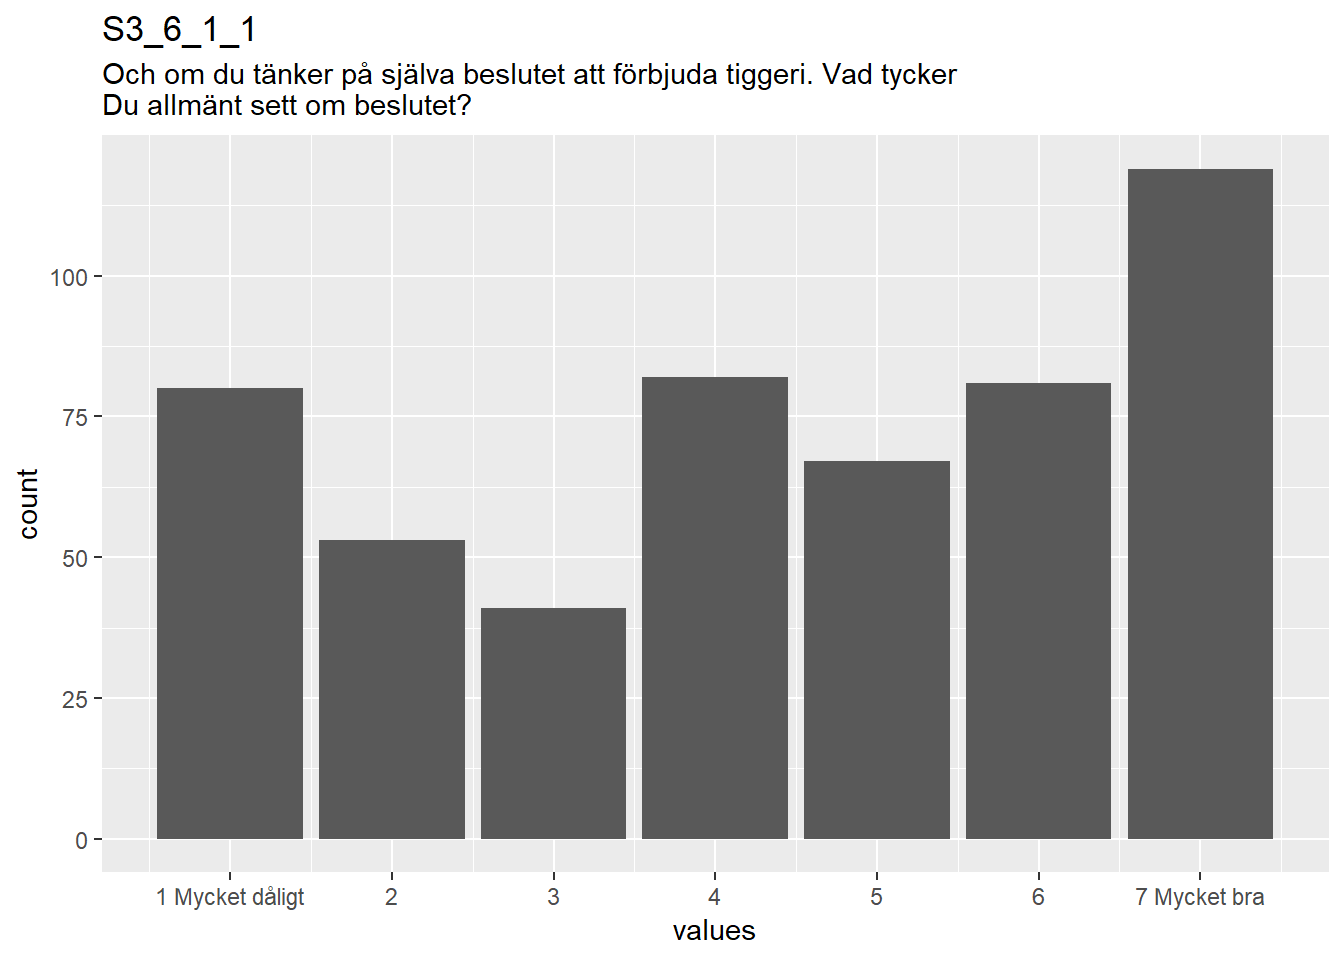
\includegraphics{Goodloser-appendix_files/figure-latex/S3_6_1_1_distribution-1.pdf}

\begin{Shaded}
\begin{Highlighting}[]
\NormalTok{knitr}\OperatorTok{::}\NormalTok{opts_chunk}\OperatorTok{$}\KeywordTok{set}\NormalTok{(}\DataTypeTok{fig.height =}\NormalTok{ old_height)}
\end{Highlighting}
\end{Shaded}

496 missings.

\subsubsection{Summary statistics}\label{S3_6_1_1_summary}

\begin{Shaded}
\begin{Highlighting}[]
\KeywordTok{attributes}\NormalTok{(item) <-}\StringTok{ }\NormalTok{item_attributes}
\NormalTok{df =}\StringTok{ }\KeywordTok{data.frame}\NormalTok{(item, }\DataTypeTok{stringsAsFactors =} \OtherTok{FALSE}\NormalTok{)}
\KeywordTok{names}\NormalTok{(df) =}\StringTok{ }\NormalTok{html_item_name}
\KeywordTok{escaped_table}\NormalTok{(}\KeywordTok{codebook_table}\NormalTok{(df))}
\end{Highlighting}
\end{Shaded}

name

label

data\_type

value\_labels

missing

complete

n

mean

sd

p0

p25

p50

p75

p100

hist

format.spss

display\_width

S3\_6\_1\_1

Och om du tänker på själva beslutet att förbjuda tiggeri. Vad tycker Du
allmänt sett om beslutet?

numeric

\begin{enumerate}
\def\labelenumi{\arabic{enumi}.}
\tightlist
\item
  1 Mycket dåligt,2. 2,3. 3,4. 4,5. 5,6. 6,7. 7 Mycket bra

  496

  523

  1019

  4.38

  2.13

  1

  2

  5

  6

  7

  ▆▃▃▆▁▅▆▇

  F1.0

  12
\end{enumerate}

\begin{Shaded}
\begin{Highlighting}[]
\ControlFlowTok{if}\NormalTok{ (show_missings) \{}
  \KeywordTok{plot_labelled}\NormalTok{(missings, item_name, wrap_at)}
\NormalTok{\}}
\end{Highlighting}
\end{Shaded}

\begin{Shaded}
\begin{Highlighting}[]
\ControlFlowTok{if}\NormalTok{ (}\OperatorTok{!}\KeywordTok{is.null}\NormalTok{(item_info)) \{}
  \CommentTok{# don't show choices again, if they're basically same thing as value labels}
  \ControlFlowTok{if}\NormalTok{ (}\OperatorTok{!}\KeywordTok{is.null}\NormalTok{(choices) }\OperatorTok{&&}\StringTok{ }\OperatorTok{!}\KeywordTok{is.null}\NormalTok{(item_info}\OperatorTok{$}\NormalTok{choices) }\OperatorTok{&&}\StringTok{ }
\StringTok{    }\KeywordTok{all}\NormalTok{(}\KeywordTok{names}\NormalTok{(}\KeywordTok{na.omit}\NormalTok{(choices)) }\OperatorTok{==}\StringTok{ }\NormalTok{item_info}\OperatorTok{$}\NormalTok{choices) }\OperatorTok{&&}
\StringTok{    }\KeywordTok{all}\NormalTok{(}\KeywordTok{na.omit}\NormalTok{(choices) }\OperatorTok{==}\StringTok{ }\KeywordTok{names}\NormalTok{(item_info}\OperatorTok{$}\NormalTok{choices))) \{}
\NormalTok{    item_info}\OperatorTok{$}\NormalTok{choices <-}\StringTok{ }\OtherTok{NULL}
\NormalTok{  \}}
\NormalTok{  item_info}\OperatorTok{$}\NormalTok{label_parsed <-}\StringTok{ }
\StringTok{    }\NormalTok{item_info}\OperatorTok{$}\NormalTok{choice_list <-}\StringTok{ }\NormalTok{item_info}\OperatorTok{$}\NormalTok{study_id <-}\StringTok{ }\NormalTok{item_info}\OperatorTok{$}\NormalTok{id <-}\StringTok{ }\OtherTok{NULL}
\NormalTok{  pander}\OperatorTok{::}\KeywordTok{pander}\NormalTok{(item_info)}
\NormalTok{\}}
\end{Highlighting}
\end{Shaded}

\subsubsection{Value labels}\label{S3_6_1_1_labels}

\begin{Shaded}
\begin{Highlighting}[]
\ControlFlowTok{if}\NormalTok{ (}\OperatorTok{!}\KeywordTok{is.null}\NormalTok{(choices) }\OperatorTok{&&}\StringTok{ }\KeywordTok{length}\NormalTok{(choices) }\OperatorTok{&&}\StringTok{ }\KeywordTok{length}\NormalTok{(choices) }\OperatorTok{<}\StringTok{ }\DecValTok{30}\NormalTok{) \{}
\NormalTok{    pander}\OperatorTok{::}\KeywordTok{pander}\NormalTok{(}\KeywordTok{as.list}\NormalTok{(choices))}
\NormalTok{\}}
\end{Highlighting}
\end{Shaded}

\begin{itemize}
\tightlist
\item
  \textbf{1 Mycket dåligt}: \emph{1}
\item
  \textbf{2}: \emph{2}
\item
  \textbf{3}: \emph{3}
\item
  \textbf{4}: \emph{4}
\item
  \textbf{5}: \emph{5}
\item
  \textbf{6}: \emph{6}
\item
  \textbf{7 Mycket bra}: \emph{7}
\end{itemize}

\subsection{S3\_6\_1\_2}\label{S3_6_1_2}

Och om du tänker på själva beslutet att inte förbjuda tiggeri. Vad
tycker Du allmänt sett om beslutet?

\subsubsection{Distribution}\label{S3_6_1_2_distribution}

\begin{Shaded}
\begin{Highlighting}[]
\NormalTok{show_missings <-}\StringTok{ }\OtherTok{FALSE}
\ControlFlowTok{if}\NormalTok{ (}\KeywordTok{has_label}\NormalTok{(item)) \{}
\NormalTok{  missings <-}\StringTok{ }\NormalTok{item[}\KeywordTok{is.na}\NormalTok{(haven}\OperatorTok{::}\KeywordTok{zap_missing}\NormalTok{(item))]}
  \KeywordTok{attributes}\NormalTok{(missings) <-}\StringTok{ }\KeywordTok{attributes}\NormalTok{(item)}
  \ControlFlowTok{if}\NormalTok{ (}\OperatorTok{!}\KeywordTok{is.null}\NormalTok{(}\KeywordTok{attributes}\NormalTok{(item)}\OperatorTok{$}\NormalTok{labels)) \{}
    \KeywordTok{attributes}\NormalTok{(missings)}\OperatorTok{$}\NormalTok{labels <-}\StringTok{ }\KeywordTok{attributes}\NormalTok{(missings)}\OperatorTok{$}\NormalTok{labels[}\KeywordTok{is.na}\NormalTok{(}\KeywordTok{attributes}\NormalTok{(missings)}\OperatorTok{$}\NormalTok{labels)]}
    \KeywordTok{attributes}\NormalTok{(item)}\OperatorTok{$}\NormalTok{labels <-}\StringTok{ }\KeywordTok{attributes}\NormalTok{(item)}\OperatorTok{$}\NormalTok{labels[}\OperatorTok{!}\KeywordTok{is.na}\NormalTok{(}\KeywordTok{attributes}\NormalTok{(item)}\OperatorTok{$}\NormalTok{labels)]}
\NormalTok{  \}}
  \ControlFlowTok{if}\NormalTok{ (}\KeywordTok{is.numeric}\NormalTok{(item)) \{}
\NormalTok{    show_missings <-}\StringTok{ }\KeywordTok{length}\NormalTok{(}\KeywordTok{unique}\NormalTok{(haven}\OperatorTok{::}\KeywordTok{na_tag}\NormalTok{(missings))) }\OperatorTok{>}\StringTok{ }\DecValTok{1}
\NormalTok{    item <-}\StringTok{ }\NormalTok{haven}\OperatorTok{::}\KeywordTok{zap_missing}\NormalTok{(item)}
\NormalTok{  \}}
  \ControlFlowTok{if}\NormalTok{ (}\KeywordTok{length}\NormalTok{(item_attributes}\OperatorTok{$}\NormalTok{labels) }\OperatorTok{==}\StringTok{ }\DecValTok{0} \OperatorTok{&&}\StringTok{ }\KeywordTok{is.numeric}\NormalTok{(item)) \{}
\NormalTok{    item <-}\StringTok{ }\NormalTok{haven}\OperatorTok{::}\KeywordTok{zap_labels}\NormalTok{(item)}
\NormalTok{  \}}
\NormalTok{\}}
\NormalTok{item_nomiss <-}\StringTok{ }\NormalTok{item[}\OperatorTok{!}\KeywordTok{is.na}\NormalTok{(item)]}

\CommentTok{# unnest mc_multiple and so on}
\ControlFlowTok{if}\NormalTok{ (}
  \KeywordTok{is.character}\NormalTok{(item_nomiss) }\OperatorTok{&&}
\StringTok{  }\NormalTok{stringr}\OperatorTok{::}\KeywordTok{str_detect}\NormalTok{(item_nomiss, stringr}\OperatorTok{::}\KeywordTok{fixed}\NormalTok{(}\StringTok{", "}\NormalTok{)) }\OperatorTok{&&}
\StringTok{  }\NormalTok{(}\KeywordTok{exists}\NormalTok{(}\StringTok{"type"}\NormalTok{, item_info) }\OperatorTok{&&}\StringTok{ }
\StringTok{    }\NormalTok{stringr}\OperatorTok{::}\KeywordTok{str_detect}\NormalTok{(item_info}\OperatorTok{$}\NormalTok{type, }\DataTypeTok{pattern =}\NormalTok{ stringr}\OperatorTok{::}\KeywordTok{fixed}\NormalTok{(}\StringTok{"multiple"}\NormalTok{)))}
\NormalTok{  ) \{}
\NormalTok{  item_nomiss <-}\StringTok{ }\KeywordTok{unlist}\NormalTok{(stringr}\OperatorTok{::}\KeywordTok{str_split}\NormalTok{(item_nomiss, }\DataTypeTok{pattern =}\NormalTok{ stringr}\OperatorTok{::}\KeywordTok{fixed}\NormalTok{(}\StringTok{", "}\NormalTok{)))}
\NormalTok{\}}
\KeywordTok{attributes}\NormalTok{(item_nomiss) <-}\StringTok{ }\KeywordTok{attributes}\NormalTok{(item)}

\NormalTok{old_height <-}\StringTok{ }\NormalTok{knitr}\OperatorTok{::}\NormalTok{opts_chunk}\OperatorTok{$}\KeywordTok{get}\NormalTok{(}\StringTok{"fig.height"}\NormalTok{)}
\NormalTok{non_missing_choices <-}\StringTok{ }\NormalTok{item_attributes[[}\StringTok{"labels"}\NormalTok{]]}
\NormalTok{many_labels <-}\StringTok{ }\KeywordTok{length}\NormalTok{(non_missing_choices) }\OperatorTok{>}\StringTok{ }\DecValTok{7}
\NormalTok{go_vertical <-}\StringTok{ }\OperatorTok{!}\KeywordTok{is.numeric}\NormalTok{(item_nomiss) }\OperatorTok{||}\StringTok{ }\NormalTok{many_labels}
\ControlFlowTok{if}\NormalTok{ ( go_vertical ) \{}
  \CommentTok{# numeric items are plotted horizontally (because that's what usually expected)}
  \CommentTok{# categorical items are plotted vertically because we can use the screen real estate better this way}

    \ControlFlowTok{if}\NormalTok{ (}\KeywordTok{is.null}\NormalTok{(choices) }\OperatorTok{||}\StringTok{ }
\StringTok{        }\NormalTok{dplyr}\OperatorTok{::}\KeywordTok{n_distinct}\NormalTok{(item_nomiss) }\OperatorTok{>}\StringTok{ }\KeywordTok{length}\NormalTok{(non_missing_choices)) \{}
\NormalTok{        non_missing_choices <-}\StringTok{ }\KeywordTok{unique}\NormalTok{(item_nomiss)}
        \KeywordTok{names}\NormalTok{(non_missing_choices) <-}\StringTok{ }\NormalTok{non_missing_choices}
\NormalTok{    \}}
\NormalTok{  choice_multiplier <-}\StringTok{ }\NormalTok{old_height}\OperatorTok{/}\FloatTok{6.5}
\NormalTok{    new_height <-}\StringTok{ }\DecValTok{2} \OperatorTok{+}\StringTok{ }\NormalTok{choice_multiplier }\OperatorTok{*}\StringTok{ }\KeywordTok{length}\NormalTok{(non_missing_choices)}
\NormalTok{    new_height <-}\StringTok{ }\KeywordTok{ifelse}\NormalTok{(new_height }\OperatorTok{>}\StringTok{ }\DecValTok{20}\NormalTok{, }\DecValTok{20}\NormalTok{, new_height)}
\NormalTok{    new_height <-}\StringTok{ }\KeywordTok{ifelse}\NormalTok{(new_height }\OperatorTok{<}\StringTok{ }\DecValTok{1}\NormalTok{, }\DecValTok{1}\NormalTok{, new_height)}
\NormalTok{    knitr}\OperatorTok{::}\NormalTok{opts_chunk}\OperatorTok{$}\KeywordTok{set}\NormalTok{(}\DataTypeTok{fig.height =}\NormalTok{ new_height)}
\NormalTok{\}}

\NormalTok{wrap_at <-}\StringTok{ }\NormalTok{knitr}\OperatorTok{::}\NormalTok{opts_chunk}\OperatorTok{$}\KeywordTok{get}\NormalTok{(}\StringTok{"fig.width"}\NormalTok{) }\OperatorTok{*}\StringTok{ }\DecValTok{10}
\end{Highlighting}
\end{Shaded}

\begin{Shaded}
\begin{Highlighting}[]
\CommentTok{# todo: if there are free-text choices mingled in with the pre-defined ones, don't show}
\CommentTok{# todo: show rare items if they are pre-defined}
\CommentTok{# todo: bin rare responses into "other category"}
\ControlFlowTok{if}\NormalTok{ (}\OperatorTok{!}\KeywordTok{length}\NormalTok{(item_nomiss)) \{}
  \KeywordTok{cat}\NormalTok{(}\StringTok{"No non-missing values to show."}\NormalTok{)}
\NormalTok{\} }\ControlFlowTok{else} \ControlFlowTok{if}\NormalTok{ (}\KeywordTok{is.numeric}\NormalTok{(item_nomiss) }\OperatorTok{||}\StringTok{ }\NormalTok{dplyr}\OperatorTok{::}\KeywordTok{n_distinct}\NormalTok{(item_nomiss) }\OperatorTok{<}\StringTok{ }\DecValTok{20}\NormalTok{) \{}
  \KeywordTok{plot_labelled}\NormalTok{(item_nomiss, item_name, wrap_at, go_vertical)}
\NormalTok{\} }\ControlFlowTok{else}\NormalTok{ \{}
    \KeywordTok{cat}\NormalTok{(dplyr}\OperatorTok{::}\KeywordTok{n_distinct}\NormalTok{(item_nomiss), }\StringTok{" unique, categorical values, so not shown."}\NormalTok{)}
\NormalTok{\}}
\end{Highlighting}
\end{Shaded}

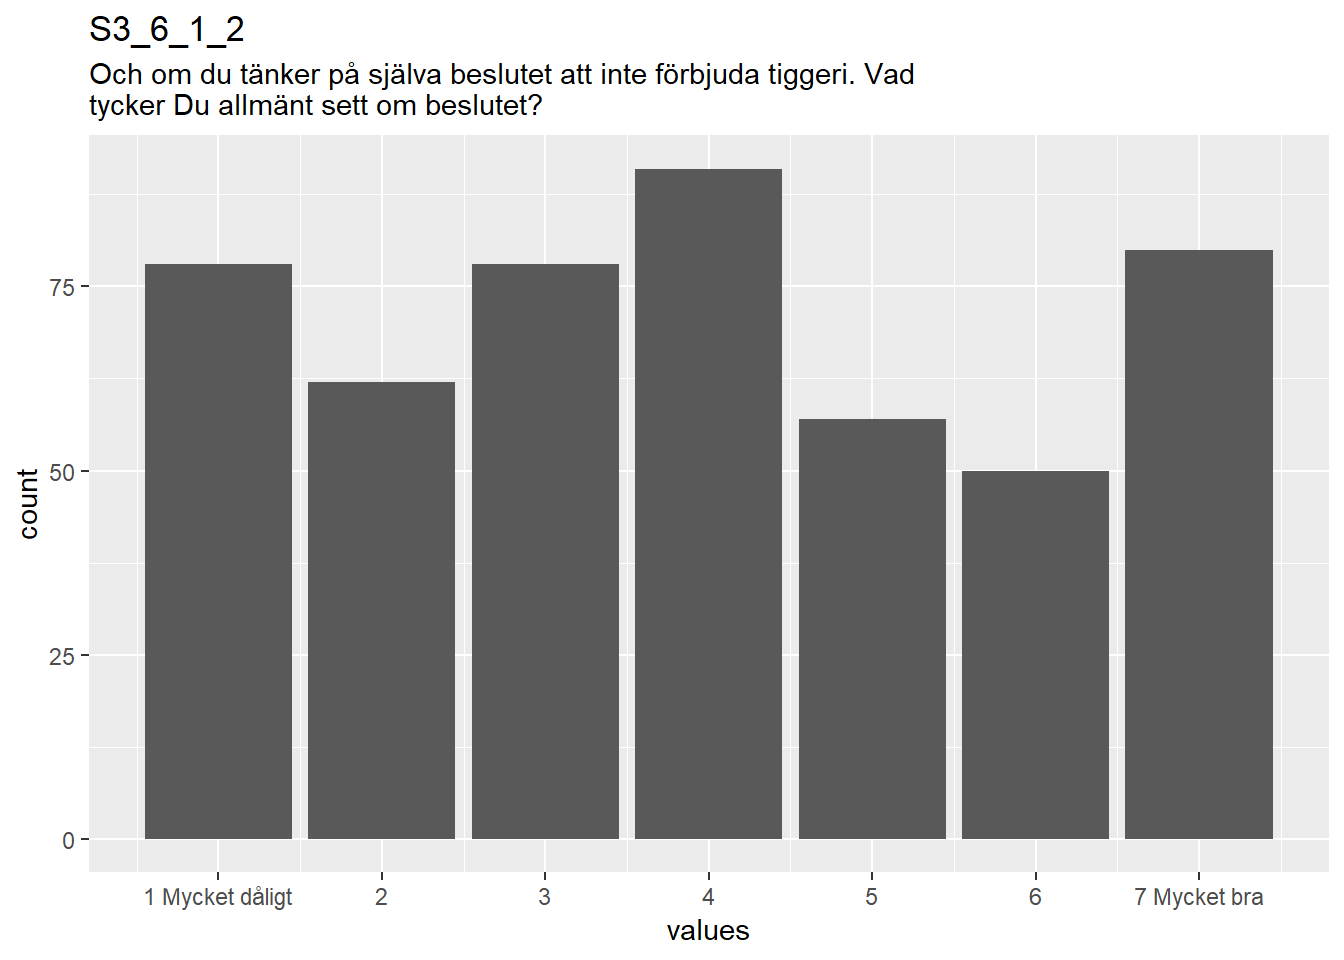
\includegraphics{Goodloser-appendix_files/figure-latex/S3_6_1_2_distribution-1.pdf}

\begin{Shaded}
\begin{Highlighting}[]
\NormalTok{knitr}\OperatorTok{::}\NormalTok{opts_chunk}\OperatorTok{$}\KeywordTok{set}\NormalTok{(}\DataTypeTok{fig.height =}\NormalTok{ old_height)}
\end{Highlighting}
\end{Shaded}

523 missings.

\subsubsection{Summary statistics}\label{S3_6_1_2_summary}

\begin{Shaded}
\begin{Highlighting}[]
\KeywordTok{attributes}\NormalTok{(item) <-}\StringTok{ }\NormalTok{item_attributes}
\NormalTok{df =}\StringTok{ }\KeywordTok{data.frame}\NormalTok{(item, }\DataTypeTok{stringsAsFactors =} \OtherTok{FALSE}\NormalTok{)}
\KeywordTok{names}\NormalTok{(df) =}\StringTok{ }\NormalTok{html_item_name}
\KeywordTok{escaped_table}\NormalTok{(}\KeywordTok{codebook_table}\NormalTok{(df))}
\end{Highlighting}
\end{Shaded}

name

label

data\_type

value\_labels

missing

complete

n

mean

sd

p0

p25

p50

p75

p100

hist

format.spss

S3\_6\_1\_2

Och om du tänker på själva beslutet att inte förbjuda tiggeri. Vad
tycker Du allmänt sett om beslutet?

numeric

\begin{enumerate}
\def\labelenumi{\arabic{enumi}.}
\tightlist
\item
  1 Mycket dåligt,2. 2,3. 3,4. 4,5. 5,6. 6,7. 7 Mycket bra

  523

  496

  1019

  3.92

  2.01

  1

  2

  4

  6

  7

  ▇▆▇▇▁▅▅▇

  F1.0
\end{enumerate}

\begin{Shaded}
\begin{Highlighting}[]
\ControlFlowTok{if}\NormalTok{ (show_missings) \{}
  \KeywordTok{plot_labelled}\NormalTok{(missings, item_name, wrap_at)}
\NormalTok{\}}
\end{Highlighting}
\end{Shaded}

\begin{Shaded}
\begin{Highlighting}[]
\ControlFlowTok{if}\NormalTok{ (}\OperatorTok{!}\KeywordTok{is.null}\NormalTok{(item_info)) \{}
  \CommentTok{# don't show choices again, if they're basically same thing as value labels}
  \ControlFlowTok{if}\NormalTok{ (}\OperatorTok{!}\KeywordTok{is.null}\NormalTok{(choices) }\OperatorTok{&&}\StringTok{ }\OperatorTok{!}\KeywordTok{is.null}\NormalTok{(item_info}\OperatorTok{$}\NormalTok{choices) }\OperatorTok{&&}\StringTok{ }
\StringTok{    }\KeywordTok{all}\NormalTok{(}\KeywordTok{names}\NormalTok{(}\KeywordTok{na.omit}\NormalTok{(choices)) }\OperatorTok{==}\StringTok{ }\NormalTok{item_info}\OperatorTok{$}\NormalTok{choices) }\OperatorTok{&&}
\StringTok{    }\KeywordTok{all}\NormalTok{(}\KeywordTok{na.omit}\NormalTok{(choices) }\OperatorTok{==}\StringTok{ }\KeywordTok{names}\NormalTok{(item_info}\OperatorTok{$}\NormalTok{choices))) \{}
\NormalTok{    item_info}\OperatorTok{$}\NormalTok{choices <-}\StringTok{ }\OtherTok{NULL}
\NormalTok{  \}}
\NormalTok{  item_info}\OperatorTok{$}\NormalTok{label_parsed <-}\StringTok{ }
\StringTok{    }\NormalTok{item_info}\OperatorTok{$}\NormalTok{choice_list <-}\StringTok{ }\NormalTok{item_info}\OperatorTok{$}\NormalTok{study_id <-}\StringTok{ }\NormalTok{item_info}\OperatorTok{$}\NormalTok{id <-}\StringTok{ }\OtherTok{NULL}
\NormalTok{  pander}\OperatorTok{::}\KeywordTok{pander}\NormalTok{(item_info)}
\NormalTok{\}}
\end{Highlighting}
\end{Shaded}

\subsubsection{Value labels}\label{S3_6_1_2_labels}

\begin{Shaded}
\begin{Highlighting}[]
\ControlFlowTok{if}\NormalTok{ (}\OperatorTok{!}\KeywordTok{is.null}\NormalTok{(choices) }\OperatorTok{&&}\StringTok{ }\KeywordTok{length}\NormalTok{(choices) }\OperatorTok{&&}\StringTok{ }\KeywordTok{length}\NormalTok{(choices) }\OperatorTok{<}\StringTok{ }\DecValTok{30}\NormalTok{) \{}
\NormalTok{    pander}\OperatorTok{::}\KeywordTok{pander}\NormalTok{(}\KeywordTok{as.list}\NormalTok{(choices))}
\NormalTok{\}}
\end{Highlighting}
\end{Shaded}

\begin{itemize}
\tightlist
\item
  \textbf{1 Mycket dåligt}: \emph{1}
\item
  \textbf{2}: \emph{2}
\item
  \textbf{3}: \emph{3}
\item
  \textbf{4}: \emph{4}
\item
  \textbf{5}: \emph{5}
\item
  \textbf{6}: \emph{6}
\item
  \textbf{7 Mycket bra}: \emph{7}
\end{itemize}

\subsection{S3\_7\_1\_1}\label{S3_7_1_1}

Hur villig är du att acceptera och följa beslutet att förbjuda tiggeri?

\subsubsection{Distribution}\label{S3_7_1_1_distribution}

\begin{Shaded}
\begin{Highlighting}[]
\NormalTok{show_missings <-}\StringTok{ }\OtherTok{FALSE}
\ControlFlowTok{if}\NormalTok{ (}\KeywordTok{has_label}\NormalTok{(item)) \{}
\NormalTok{  missings <-}\StringTok{ }\NormalTok{item[}\KeywordTok{is.na}\NormalTok{(haven}\OperatorTok{::}\KeywordTok{zap_missing}\NormalTok{(item))]}
  \KeywordTok{attributes}\NormalTok{(missings) <-}\StringTok{ }\KeywordTok{attributes}\NormalTok{(item)}
  \ControlFlowTok{if}\NormalTok{ (}\OperatorTok{!}\KeywordTok{is.null}\NormalTok{(}\KeywordTok{attributes}\NormalTok{(item)}\OperatorTok{$}\NormalTok{labels)) \{}
    \KeywordTok{attributes}\NormalTok{(missings)}\OperatorTok{$}\NormalTok{labels <-}\StringTok{ }\KeywordTok{attributes}\NormalTok{(missings)}\OperatorTok{$}\NormalTok{labels[}\KeywordTok{is.na}\NormalTok{(}\KeywordTok{attributes}\NormalTok{(missings)}\OperatorTok{$}\NormalTok{labels)]}
    \KeywordTok{attributes}\NormalTok{(item)}\OperatorTok{$}\NormalTok{labels <-}\StringTok{ }\KeywordTok{attributes}\NormalTok{(item)}\OperatorTok{$}\NormalTok{labels[}\OperatorTok{!}\KeywordTok{is.na}\NormalTok{(}\KeywordTok{attributes}\NormalTok{(item)}\OperatorTok{$}\NormalTok{labels)]}
\NormalTok{  \}}
  \ControlFlowTok{if}\NormalTok{ (}\KeywordTok{is.numeric}\NormalTok{(item)) \{}
\NormalTok{    show_missings <-}\StringTok{ }\KeywordTok{length}\NormalTok{(}\KeywordTok{unique}\NormalTok{(haven}\OperatorTok{::}\KeywordTok{na_tag}\NormalTok{(missings))) }\OperatorTok{>}\StringTok{ }\DecValTok{1}
\NormalTok{    item <-}\StringTok{ }\NormalTok{haven}\OperatorTok{::}\KeywordTok{zap_missing}\NormalTok{(item)}
\NormalTok{  \}}
  \ControlFlowTok{if}\NormalTok{ (}\KeywordTok{length}\NormalTok{(item_attributes}\OperatorTok{$}\NormalTok{labels) }\OperatorTok{==}\StringTok{ }\DecValTok{0} \OperatorTok{&&}\StringTok{ }\KeywordTok{is.numeric}\NormalTok{(item)) \{}
\NormalTok{    item <-}\StringTok{ }\NormalTok{haven}\OperatorTok{::}\KeywordTok{zap_labels}\NormalTok{(item)}
\NormalTok{  \}}
\NormalTok{\}}
\NormalTok{item_nomiss <-}\StringTok{ }\NormalTok{item[}\OperatorTok{!}\KeywordTok{is.na}\NormalTok{(item)]}

\CommentTok{# unnest mc_multiple and so on}
\ControlFlowTok{if}\NormalTok{ (}
  \KeywordTok{is.character}\NormalTok{(item_nomiss) }\OperatorTok{&&}
\StringTok{  }\NormalTok{stringr}\OperatorTok{::}\KeywordTok{str_detect}\NormalTok{(item_nomiss, stringr}\OperatorTok{::}\KeywordTok{fixed}\NormalTok{(}\StringTok{", "}\NormalTok{)) }\OperatorTok{&&}
\StringTok{  }\NormalTok{(}\KeywordTok{exists}\NormalTok{(}\StringTok{"type"}\NormalTok{, item_info) }\OperatorTok{&&}\StringTok{ }
\StringTok{    }\NormalTok{stringr}\OperatorTok{::}\KeywordTok{str_detect}\NormalTok{(item_info}\OperatorTok{$}\NormalTok{type, }\DataTypeTok{pattern =}\NormalTok{ stringr}\OperatorTok{::}\KeywordTok{fixed}\NormalTok{(}\StringTok{"multiple"}\NormalTok{)))}
\NormalTok{  ) \{}
\NormalTok{  item_nomiss <-}\StringTok{ }\KeywordTok{unlist}\NormalTok{(stringr}\OperatorTok{::}\KeywordTok{str_split}\NormalTok{(item_nomiss, }\DataTypeTok{pattern =}\NormalTok{ stringr}\OperatorTok{::}\KeywordTok{fixed}\NormalTok{(}\StringTok{", "}\NormalTok{)))}
\NormalTok{\}}
\KeywordTok{attributes}\NormalTok{(item_nomiss) <-}\StringTok{ }\KeywordTok{attributes}\NormalTok{(item)}

\NormalTok{old_height <-}\StringTok{ }\NormalTok{knitr}\OperatorTok{::}\NormalTok{opts_chunk}\OperatorTok{$}\KeywordTok{get}\NormalTok{(}\StringTok{"fig.height"}\NormalTok{)}
\NormalTok{non_missing_choices <-}\StringTok{ }\NormalTok{item_attributes[[}\StringTok{"labels"}\NormalTok{]]}
\NormalTok{many_labels <-}\StringTok{ }\KeywordTok{length}\NormalTok{(non_missing_choices) }\OperatorTok{>}\StringTok{ }\DecValTok{7}
\NormalTok{go_vertical <-}\StringTok{ }\OperatorTok{!}\KeywordTok{is.numeric}\NormalTok{(item_nomiss) }\OperatorTok{||}\StringTok{ }\NormalTok{many_labels}
\ControlFlowTok{if}\NormalTok{ ( go_vertical ) \{}
  \CommentTok{# numeric items are plotted horizontally (because that's what usually expected)}
  \CommentTok{# categorical items are plotted vertically because we can use the screen real estate better this way}

    \ControlFlowTok{if}\NormalTok{ (}\KeywordTok{is.null}\NormalTok{(choices) }\OperatorTok{||}\StringTok{ }
\StringTok{        }\NormalTok{dplyr}\OperatorTok{::}\KeywordTok{n_distinct}\NormalTok{(item_nomiss) }\OperatorTok{>}\StringTok{ }\KeywordTok{length}\NormalTok{(non_missing_choices)) \{}
\NormalTok{        non_missing_choices <-}\StringTok{ }\KeywordTok{unique}\NormalTok{(item_nomiss)}
        \KeywordTok{names}\NormalTok{(non_missing_choices) <-}\StringTok{ }\NormalTok{non_missing_choices}
\NormalTok{    \}}
\NormalTok{  choice_multiplier <-}\StringTok{ }\NormalTok{old_height}\OperatorTok{/}\FloatTok{6.5}
\NormalTok{    new_height <-}\StringTok{ }\DecValTok{2} \OperatorTok{+}\StringTok{ }\NormalTok{choice_multiplier }\OperatorTok{*}\StringTok{ }\KeywordTok{length}\NormalTok{(non_missing_choices)}
\NormalTok{    new_height <-}\StringTok{ }\KeywordTok{ifelse}\NormalTok{(new_height }\OperatorTok{>}\StringTok{ }\DecValTok{20}\NormalTok{, }\DecValTok{20}\NormalTok{, new_height)}
\NormalTok{    new_height <-}\StringTok{ }\KeywordTok{ifelse}\NormalTok{(new_height }\OperatorTok{<}\StringTok{ }\DecValTok{1}\NormalTok{, }\DecValTok{1}\NormalTok{, new_height)}
\NormalTok{    knitr}\OperatorTok{::}\NormalTok{opts_chunk}\OperatorTok{$}\KeywordTok{set}\NormalTok{(}\DataTypeTok{fig.height =}\NormalTok{ new_height)}
\NormalTok{\}}

\NormalTok{wrap_at <-}\StringTok{ }\NormalTok{knitr}\OperatorTok{::}\NormalTok{opts_chunk}\OperatorTok{$}\KeywordTok{get}\NormalTok{(}\StringTok{"fig.width"}\NormalTok{) }\OperatorTok{*}\StringTok{ }\DecValTok{10}
\end{Highlighting}
\end{Shaded}

\begin{Shaded}
\begin{Highlighting}[]
\CommentTok{# todo: if there are free-text choices mingled in with the pre-defined ones, don't show}
\CommentTok{# todo: show rare items if they are pre-defined}
\CommentTok{# todo: bin rare responses into "other category"}
\ControlFlowTok{if}\NormalTok{ (}\OperatorTok{!}\KeywordTok{length}\NormalTok{(item_nomiss)) \{}
  \KeywordTok{cat}\NormalTok{(}\StringTok{"No non-missing values to show."}\NormalTok{)}
\NormalTok{\} }\ControlFlowTok{else} \ControlFlowTok{if}\NormalTok{ (}\KeywordTok{is.numeric}\NormalTok{(item_nomiss) }\OperatorTok{||}\StringTok{ }\NormalTok{dplyr}\OperatorTok{::}\KeywordTok{n_distinct}\NormalTok{(item_nomiss) }\OperatorTok{<}\StringTok{ }\DecValTok{20}\NormalTok{) \{}
  \KeywordTok{plot_labelled}\NormalTok{(item_nomiss, item_name, wrap_at, go_vertical)}
\NormalTok{\} }\ControlFlowTok{else}\NormalTok{ \{}
    \KeywordTok{cat}\NormalTok{(dplyr}\OperatorTok{::}\KeywordTok{n_distinct}\NormalTok{(item_nomiss), }\StringTok{" unique, categorical values, so not shown."}\NormalTok{)}
\NormalTok{\}}
\end{Highlighting}
\end{Shaded}

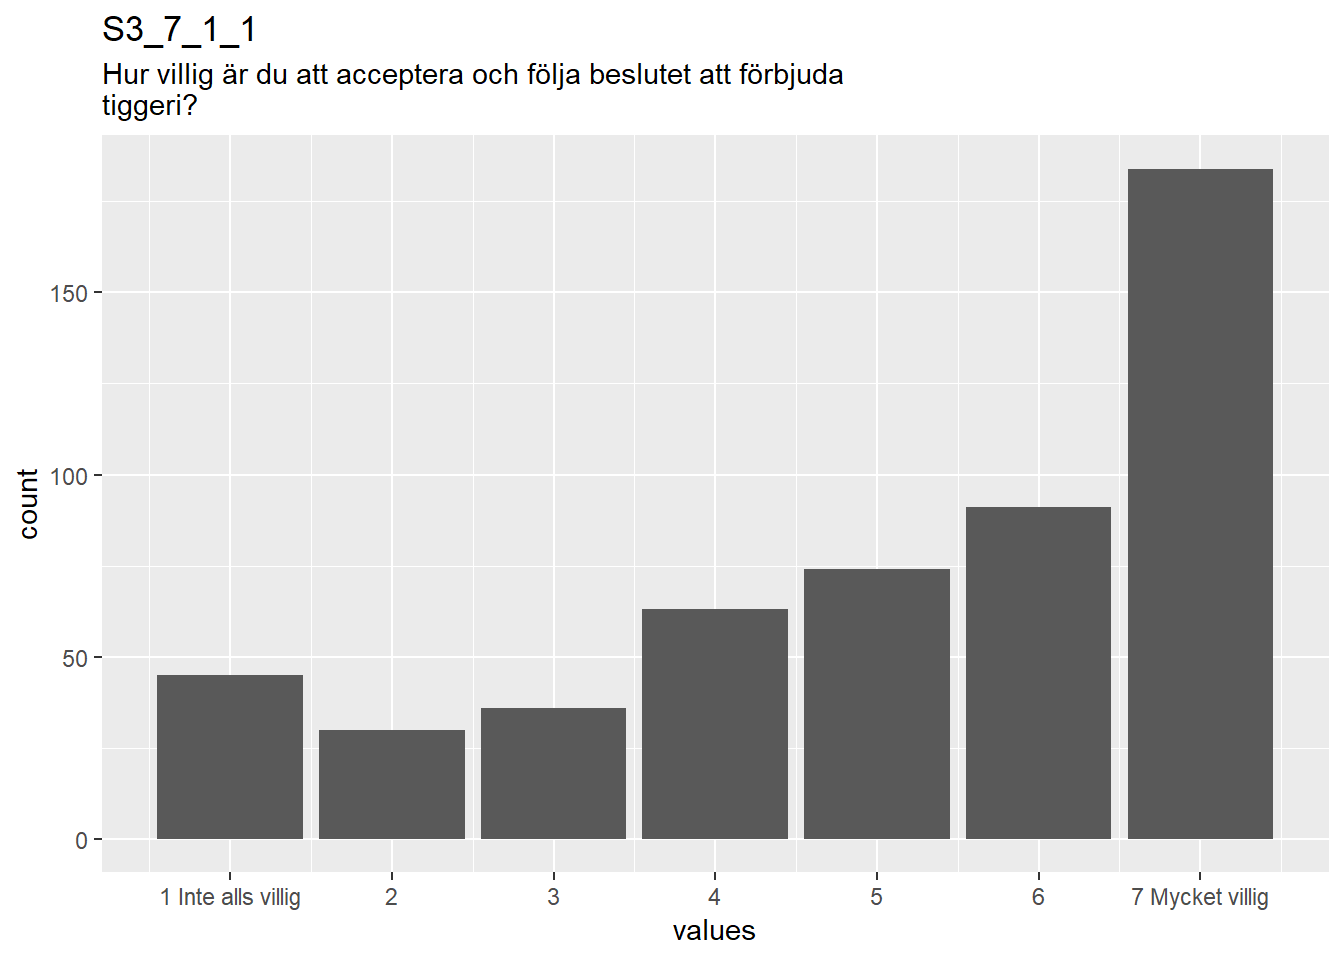
\includegraphics{Goodloser-appendix_files/figure-latex/S3_7_1_1_distribution-1.pdf}

\begin{Shaded}
\begin{Highlighting}[]
\NormalTok{knitr}\OperatorTok{::}\NormalTok{opts_chunk}\OperatorTok{$}\KeywordTok{set}\NormalTok{(}\DataTypeTok{fig.height =}\NormalTok{ old_height)}
\end{Highlighting}
\end{Shaded}

496 missings.

\subsubsection{Summary statistics}\label{S3_7_1_1_summary}

\begin{Shaded}
\begin{Highlighting}[]
\KeywordTok{attributes}\NormalTok{(item) <-}\StringTok{ }\NormalTok{item_attributes}
\NormalTok{df =}\StringTok{ }\KeywordTok{data.frame}\NormalTok{(item, }\DataTypeTok{stringsAsFactors =} \OtherTok{FALSE}\NormalTok{)}
\KeywordTok{names}\NormalTok{(df) =}\StringTok{ }\NormalTok{html_item_name}
\KeywordTok{escaped_table}\NormalTok{(}\KeywordTok{codebook_table}\NormalTok{(df))}
\end{Highlighting}
\end{Shaded}

name

label

data\_type

value\_labels

missing

complete

n

mean

sd

p0

p25

p50

p75

p100

hist

format.spss

display\_width

S3\_7\_1\_1

Hur villig är du att acceptera och följa beslutet att förbjuda tiggeri?

numeric

\begin{enumerate}
\def\labelenumi{\arabic{enumi}.}
\tightlist
\item
  1 Inte alls villig,2. 2,3. 3,4. 4,5. 5,6. 6,7. 7 Mycket villig

  496

  523

  1019

  5.1

  1.97

  1

  4

  6

  7

  7

  ▂▁▂▃▁▃▃▇

  F1.0

  12
\end{enumerate}

\begin{Shaded}
\begin{Highlighting}[]
\ControlFlowTok{if}\NormalTok{ (show_missings) \{}
  \KeywordTok{plot_labelled}\NormalTok{(missings, item_name, wrap_at)}
\NormalTok{\}}
\end{Highlighting}
\end{Shaded}

\begin{Shaded}
\begin{Highlighting}[]
\ControlFlowTok{if}\NormalTok{ (}\OperatorTok{!}\KeywordTok{is.null}\NormalTok{(item_info)) \{}
  \CommentTok{# don't show choices again, if they're basically same thing as value labels}
  \ControlFlowTok{if}\NormalTok{ (}\OperatorTok{!}\KeywordTok{is.null}\NormalTok{(choices) }\OperatorTok{&&}\StringTok{ }\OperatorTok{!}\KeywordTok{is.null}\NormalTok{(item_info}\OperatorTok{$}\NormalTok{choices) }\OperatorTok{&&}\StringTok{ }
\StringTok{    }\KeywordTok{all}\NormalTok{(}\KeywordTok{names}\NormalTok{(}\KeywordTok{na.omit}\NormalTok{(choices)) }\OperatorTok{==}\StringTok{ }\NormalTok{item_info}\OperatorTok{$}\NormalTok{choices) }\OperatorTok{&&}
\StringTok{    }\KeywordTok{all}\NormalTok{(}\KeywordTok{na.omit}\NormalTok{(choices) }\OperatorTok{==}\StringTok{ }\KeywordTok{names}\NormalTok{(item_info}\OperatorTok{$}\NormalTok{choices))) \{}
\NormalTok{    item_info}\OperatorTok{$}\NormalTok{choices <-}\StringTok{ }\OtherTok{NULL}
\NormalTok{  \}}
\NormalTok{  item_info}\OperatorTok{$}\NormalTok{label_parsed <-}\StringTok{ }
\StringTok{    }\NormalTok{item_info}\OperatorTok{$}\NormalTok{choice_list <-}\StringTok{ }\NormalTok{item_info}\OperatorTok{$}\NormalTok{study_id <-}\StringTok{ }\NormalTok{item_info}\OperatorTok{$}\NormalTok{id <-}\StringTok{ }\OtherTok{NULL}
\NormalTok{  pander}\OperatorTok{::}\KeywordTok{pander}\NormalTok{(item_info)}
\NormalTok{\}}
\end{Highlighting}
\end{Shaded}

\subsubsection{Value labels}\label{S3_7_1_1_labels}

\begin{Shaded}
\begin{Highlighting}[]
\ControlFlowTok{if}\NormalTok{ (}\OperatorTok{!}\KeywordTok{is.null}\NormalTok{(choices) }\OperatorTok{&&}\StringTok{ }\KeywordTok{length}\NormalTok{(choices) }\OperatorTok{&&}\StringTok{ }\KeywordTok{length}\NormalTok{(choices) }\OperatorTok{<}\StringTok{ }\DecValTok{30}\NormalTok{) \{}
\NormalTok{    pander}\OperatorTok{::}\KeywordTok{pander}\NormalTok{(}\KeywordTok{as.list}\NormalTok{(choices))}
\NormalTok{\}}
\end{Highlighting}
\end{Shaded}

\begin{itemize}
\tightlist
\item
  \textbf{1 Inte alls villig}: \emph{1}
\item
  \textbf{2}: \emph{2}
\item
  \textbf{3}: \emph{3}
\item
  \textbf{4}: \emph{4}
\item
  \textbf{5}: \emph{5}
\item
  \textbf{6}: \emph{6}
\item
  \textbf{7 Mycket villig}: \emph{7}
\end{itemize}

\subsection{S3\_7\_1\_2}\label{S3_7_1_2}

Hur villig är du att acceptera och följa beslutet att inte förbjuda
tiggeri?

\subsubsection{Distribution}\label{S3_7_1_2_distribution}

\begin{Shaded}
\begin{Highlighting}[]
\NormalTok{show_missings <-}\StringTok{ }\OtherTok{FALSE}
\ControlFlowTok{if}\NormalTok{ (}\KeywordTok{has_label}\NormalTok{(item)) \{}
\NormalTok{  missings <-}\StringTok{ }\NormalTok{item[}\KeywordTok{is.na}\NormalTok{(haven}\OperatorTok{::}\KeywordTok{zap_missing}\NormalTok{(item))]}
  \KeywordTok{attributes}\NormalTok{(missings) <-}\StringTok{ }\KeywordTok{attributes}\NormalTok{(item)}
  \ControlFlowTok{if}\NormalTok{ (}\OperatorTok{!}\KeywordTok{is.null}\NormalTok{(}\KeywordTok{attributes}\NormalTok{(item)}\OperatorTok{$}\NormalTok{labels)) \{}
    \KeywordTok{attributes}\NormalTok{(missings)}\OperatorTok{$}\NormalTok{labels <-}\StringTok{ }\KeywordTok{attributes}\NormalTok{(missings)}\OperatorTok{$}\NormalTok{labels[}\KeywordTok{is.na}\NormalTok{(}\KeywordTok{attributes}\NormalTok{(missings)}\OperatorTok{$}\NormalTok{labels)]}
    \KeywordTok{attributes}\NormalTok{(item)}\OperatorTok{$}\NormalTok{labels <-}\StringTok{ }\KeywordTok{attributes}\NormalTok{(item)}\OperatorTok{$}\NormalTok{labels[}\OperatorTok{!}\KeywordTok{is.na}\NormalTok{(}\KeywordTok{attributes}\NormalTok{(item)}\OperatorTok{$}\NormalTok{labels)]}
\NormalTok{  \}}
  \ControlFlowTok{if}\NormalTok{ (}\KeywordTok{is.numeric}\NormalTok{(item)) \{}
\NormalTok{    show_missings <-}\StringTok{ }\KeywordTok{length}\NormalTok{(}\KeywordTok{unique}\NormalTok{(haven}\OperatorTok{::}\KeywordTok{na_tag}\NormalTok{(missings))) }\OperatorTok{>}\StringTok{ }\DecValTok{1}
\NormalTok{    item <-}\StringTok{ }\NormalTok{haven}\OperatorTok{::}\KeywordTok{zap_missing}\NormalTok{(item)}
\NormalTok{  \}}
  \ControlFlowTok{if}\NormalTok{ (}\KeywordTok{length}\NormalTok{(item_attributes}\OperatorTok{$}\NormalTok{labels) }\OperatorTok{==}\StringTok{ }\DecValTok{0} \OperatorTok{&&}\StringTok{ }\KeywordTok{is.numeric}\NormalTok{(item)) \{}
\NormalTok{    item <-}\StringTok{ }\NormalTok{haven}\OperatorTok{::}\KeywordTok{zap_labels}\NormalTok{(item)}
\NormalTok{  \}}
\NormalTok{\}}
\NormalTok{item_nomiss <-}\StringTok{ }\NormalTok{item[}\OperatorTok{!}\KeywordTok{is.na}\NormalTok{(item)]}

\CommentTok{# unnest mc_multiple and so on}
\ControlFlowTok{if}\NormalTok{ (}
  \KeywordTok{is.character}\NormalTok{(item_nomiss) }\OperatorTok{&&}
\StringTok{  }\NormalTok{stringr}\OperatorTok{::}\KeywordTok{str_detect}\NormalTok{(item_nomiss, stringr}\OperatorTok{::}\KeywordTok{fixed}\NormalTok{(}\StringTok{", "}\NormalTok{)) }\OperatorTok{&&}
\StringTok{  }\NormalTok{(}\KeywordTok{exists}\NormalTok{(}\StringTok{"type"}\NormalTok{, item_info) }\OperatorTok{&&}\StringTok{ }
\StringTok{    }\NormalTok{stringr}\OperatorTok{::}\KeywordTok{str_detect}\NormalTok{(item_info}\OperatorTok{$}\NormalTok{type, }\DataTypeTok{pattern =}\NormalTok{ stringr}\OperatorTok{::}\KeywordTok{fixed}\NormalTok{(}\StringTok{"multiple"}\NormalTok{)))}
\NormalTok{  ) \{}
\NormalTok{  item_nomiss <-}\StringTok{ }\KeywordTok{unlist}\NormalTok{(stringr}\OperatorTok{::}\KeywordTok{str_split}\NormalTok{(item_nomiss, }\DataTypeTok{pattern =}\NormalTok{ stringr}\OperatorTok{::}\KeywordTok{fixed}\NormalTok{(}\StringTok{", "}\NormalTok{)))}
\NormalTok{\}}
\KeywordTok{attributes}\NormalTok{(item_nomiss) <-}\StringTok{ }\KeywordTok{attributes}\NormalTok{(item)}

\NormalTok{old_height <-}\StringTok{ }\NormalTok{knitr}\OperatorTok{::}\NormalTok{opts_chunk}\OperatorTok{$}\KeywordTok{get}\NormalTok{(}\StringTok{"fig.height"}\NormalTok{)}
\NormalTok{non_missing_choices <-}\StringTok{ }\NormalTok{item_attributes[[}\StringTok{"labels"}\NormalTok{]]}
\NormalTok{many_labels <-}\StringTok{ }\KeywordTok{length}\NormalTok{(non_missing_choices) }\OperatorTok{>}\StringTok{ }\DecValTok{7}
\NormalTok{go_vertical <-}\StringTok{ }\OperatorTok{!}\KeywordTok{is.numeric}\NormalTok{(item_nomiss) }\OperatorTok{||}\StringTok{ }\NormalTok{many_labels}
\ControlFlowTok{if}\NormalTok{ ( go_vertical ) \{}
  \CommentTok{# numeric items are plotted horizontally (because that's what usually expected)}
  \CommentTok{# categorical items are plotted vertically because we can use the screen real estate better this way}

    \ControlFlowTok{if}\NormalTok{ (}\KeywordTok{is.null}\NormalTok{(choices) }\OperatorTok{||}\StringTok{ }
\StringTok{        }\NormalTok{dplyr}\OperatorTok{::}\KeywordTok{n_distinct}\NormalTok{(item_nomiss) }\OperatorTok{>}\StringTok{ }\KeywordTok{length}\NormalTok{(non_missing_choices)) \{}
\NormalTok{        non_missing_choices <-}\StringTok{ }\KeywordTok{unique}\NormalTok{(item_nomiss)}
        \KeywordTok{names}\NormalTok{(non_missing_choices) <-}\StringTok{ }\NormalTok{non_missing_choices}
\NormalTok{    \}}
\NormalTok{  choice_multiplier <-}\StringTok{ }\NormalTok{old_height}\OperatorTok{/}\FloatTok{6.5}
\NormalTok{    new_height <-}\StringTok{ }\DecValTok{2} \OperatorTok{+}\StringTok{ }\NormalTok{choice_multiplier }\OperatorTok{*}\StringTok{ }\KeywordTok{length}\NormalTok{(non_missing_choices)}
\NormalTok{    new_height <-}\StringTok{ }\KeywordTok{ifelse}\NormalTok{(new_height }\OperatorTok{>}\StringTok{ }\DecValTok{20}\NormalTok{, }\DecValTok{20}\NormalTok{, new_height)}
\NormalTok{    new_height <-}\StringTok{ }\KeywordTok{ifelse}\NormalTok{(new_height }\OperatorTok{<}\StringTok{ }\DecValTok{1}\NormalTok{, }\DecValTok{1}\NormalTok{, new_height)}
\NormalTok{    knitr}\OperatorTok{::}\NormalTok{opts_chunk}\OperatorTok{$}\KeywordTok{set}\NormalTok{(}\DataTypeTok{fig.height =}\NormalTok{ new_height)}
\NormalTok{\}}

\NormalTok{wrap_at <-}\StringTok{ }\NormalTok{knitr}\OperatorTok{::}\NormalTok{opts_chunk}\OperatorTok{$}\KeywordTok{get}\NormalTok{(}\StringTok{"fig.width"}\NormalTok{) }\OperatorTok{*}\StringTok{ }\DecValTok{10}
\end{Highlighting}
\end{Shaded}

\begin{Shaded}
\begin{Highlighting}[]
\CommentTok{# todo: if there are free-text choices mingled in with the pre-defined ones, don't show}
\CommentTok{# todo: show rare items if they are pre-defined}
\CommentTok{# todo: bin rare responses into "other category"}
\ControlFlowTok{if}\NormalTok{ (}\OperatorTok{!}\KeywordTok{length}\NormalTok{(item_nomiss)) \{}
  \KeywordTok{cat}\NormalTok{(}\StringTok{"No non-missing values to show."}\NormalTok{)}
\NormalTok{\} }\ControlFlowTok{else} \ControlFlowTok{if}\NormalTok{ (}\KeywordTok{is.numeric}\NormalTok{(item_nomiss) }\OperatorTok{||}\StringTok{ }\NormalTok{dplyr}\OperatorTok{::}\KeywordTok{n_distinct}\NormalTok{(item_nomiss) }\OperatorTok{<}\StringTok{ }\DecValTok{20}\NormalTok{) \{}
  \KeywordTok{plot_labelled}\NormalTok{(item_nomiss, item_name, wrap_at, go_vertical)}
\NormalTok{\} }\ControlFlowTok{else}\NormalTok{ \{}
    \KeywordTok{cat}\NormalTok{(dplyr}\OperatorTok{::}\KeywordTok{n_distinct}\NormalTok{(item_nomiss), }\StringTok{" unique, categorical values, so not shown."}\NormalTok{)}
\NormalTok{\}}
\end{Highlighting}
\end{Shaded}

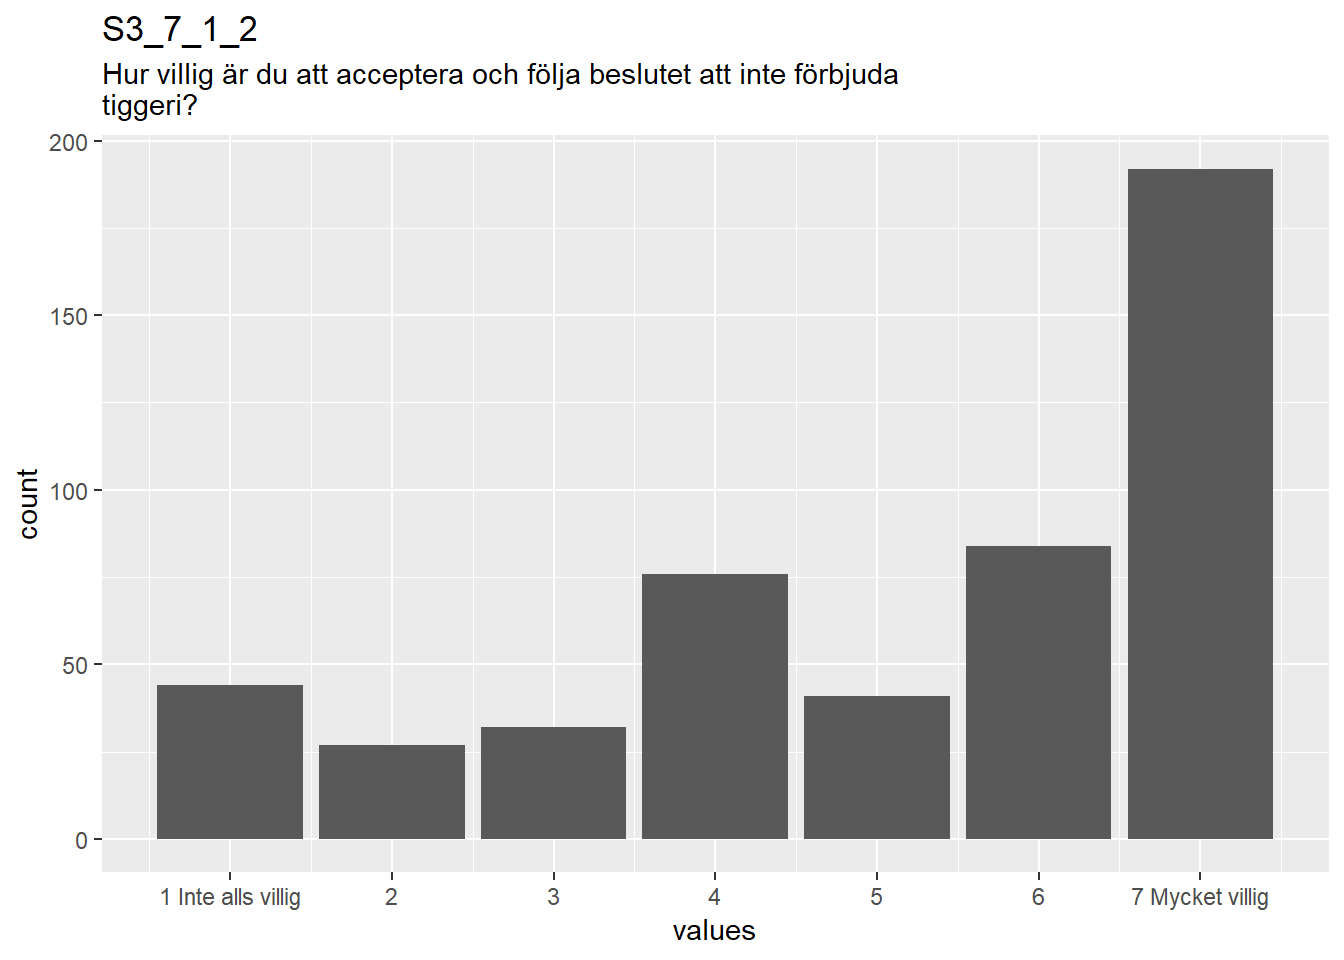
\includegraphics{Goodloser-appendix_files/figure-latex/S3_7_1_2_distribution-1.pdf}

\begin{Shaded}
\begin{Highlighting}[]
\NormalTok{knitr}\OperatorTok{::}\NormalTok{opts_chunk}\OperatorTok{$}\KeywordTok{set}\NormalTok{(}\DataTypeTok{fig.height =}\NormalTok{ old_height)}
\end{Highlighting}
\end{Shaded}

523 missings.

\subsubsection{Summary statistics}\label{S3_7_1_2_summary}

\begin{Shaded}
\begin{Highlighting}[]
\KeywordTok{attributes}\NormalTok{(item) <-}\StringTok{ }\NormalTok{item_attributes}
\NormalTok{df =}\StringTok{ }\KeywordTok{data.frame}\NormalTok{(item, }\DataTypeTok{stringsAsFactors =} \OtherTok{FALSE}\NormalTok{)}
\KeywordTok{names}\NormalTok{(df) =}\StringTok{ }\NormalTok{html_item_name}
\KeywordTok{escaped_table}\NormalTok{(}\KeywordTok{codebook_table}\NormalTok{(df))}
\end{Highlighting}
\end{Shaded}

name

label

data\_type

value\_labels

missing

complete

n

mean

sd

p0

p25

p50

p75

p100

hist

format.spss

S3\_7\_1\_2

Hur villig är du att acceptera och följa beslutet att inte förbjuda
tiggeri?

numeric

\begin{enumerate}
\def\labelenumi{\arabic{enumi}.}
\tightlist
\item
  1 Inte alls villig,2. 2,3. 3,4. 4,5. 5,6. 6,7. 7 Mycket villig

  523

  496

  1019

  5.14

  2.01

  1

  4

  6

  7

  7

  ▂▁▁▃▁▂▃▇

  F1.0
\end{enumerate}

\begin{Shaded}
\begin{Highlighting}[]
\ControlFlowTok{if}\NormalTok{ (show_missings) \{}
  \KeywordTok{plot_labelled}\NormalTok{(missings, item_name, wrap_at)}
\NormalTok{\}}
\end{Highlighting}
\end{Shaded}

\begin{Shaded}
\begin{Highlighting}[]
\ControlFlowTok{if}\NormalTok{ (}\OperatorTok{!}\KeywordTok{is.null}\NormalTok{(item_info)) \{}
  \CommentTok{# don't show choices again, if they're basically same thing as value labels}
  \ControlFlowTok{if}\NormalTok{ (}\OperatorTok{!}\KeywordTok{is.null}\NormalTok{(choices) }\OperatorTok{&&}\StringTok{ }\OperatorTok{!}\KeywordTok{is.null}\NormalTok{(item_info}\OperatorTok{$}\NormalTok{choices) }\OperatorTok{&&}\StringTok{ }
\StringTok{    }\KeywordTok{all}\NormalTok{(}\KeywordTok{names}\NormalTok{(}\KeywordTok{na.omit}\NormalTok{(choices)) }\OperatorTok{==}\StringTok{ }\NormalTok{item_info}\OperatorTok{$}\NormalTok{choices) }\OperatorTok{&&}
\StringTok{    }\KeywordTok{all}\NormalTok{(}\KeywordTok{na.omit}\NormalTok{(choices) }\OperatorTok{==}\StringTok{ }\KeywordTok{names}\NormalTok{(item_info}\OperatorTok{$}\NormalTok{choices))) \{}
\NormalTok{    item_info}\OperatorTok{$}\NormalTok{choices <-}\StringTok{ }\OtherTok{NULL}
\NormalTok{  \}}
\NormalTok{  item_info}\OperatorTok{$}\NormalTok{label_parsed <-}\StringTok{ }
\StringTok{    }\NormalTok{item_info}\OperatorTok{$}\NormalTok{choice_list <-}\StringTok{ }\NormalTok{item_info}\OperatorTok{$}\NormalTok{study_id <-}\StringTok{ }\NormalTok{item_info}\OperatorTok{$}\NormalTok{id <-}\StringTok{ }\OtherTok{NULL}
\NormalTok{  pander}\OperatorTok{::}\KeywordTok{pander}\NormalTok{(item_info)}
\NormalTok{\}}
\end{Highlighting}
\end{Shaded}

\subsubsection{Value labels}\label{S3_7_1_2_labels}

\begin{Shaded}
\begin{Highlighting}[]
\ControlFlowTok{if}\NormalTok{ (}\OperatorTok{!}\KeywordTok{is.null}\NormalTok{(choices) }\OperatorTok{&&}\StringTok{ }\KeywordTok{length}\NormalTok{(choices) }\OperatorTok{&&}\StringTok{ }\KeywordTok{length}\NormalTok{(choices) }\OperatorTok{<}\StringTok{ }\DecValTok{30}\NormalTok{) \{}
\NormalTok{    pander}\OperatorTok{::}\KeywordTok{pander}\NormalTok{(}\KeywordTok{as.list}\NormalTok{(choices))}
\NormalTok{\}}
\end{Highlighting}
\end{Shaded}

\begin{itemize}
\tightlist
\item
  \textbf{1 Inte alls villig}: \emph{1}
\item
  \textbf{2}: \emph{2}
\item
  \textbf{3}: \emph{3}
\item
  \textbf{4}: \emph{4}
\item
  \textbf{5}: \emph{5}
\item
  \textbf{6}: \emph{6}
\item
  \textbf{7 Mycket villig}: \emph{7}
\end{itemize}

\subsection{S3\_8\_1\_1}\label{S3_8_1_1}

När det gäller att följa eller motarbeta beslutet att förbjuda tiggeri,
var på skalan skulle du placera dig?

\subsubsection{Distribution}\label{S3_8_1_1_distribution}

\begin{Shaded}
\begin{Highlighting}[]
\NormalTok{show_missings <-}\StringTok{ }\OtherTok{FALSE}
\ControlFlowTok{if}\NormalTok{ (}\KeywordTok{has_label}\NormalTok{(item)) \{}
\NormalTok{  missings <-}\StringTok{ }\NormalTok{item[}\KeywordTok{is.na}\NormalTok{(haven}\OperatorTok{::}\KeywordTok{zap_missing}\NormalTok{(item))]}
  \KeywordTok{attributes}\NormalTok{(missings) <-}\StringTok{ }\KeywordTok{attributes}\NormalTok{(item)}
  \ControlFlowTok{if}\NormalTok{ (}\OperatorTok{!}\KeywordTok{is.null}\NormalTok{(}\KeywordTok{attributes}\NormalTok{(item)}\OperatorTok{$}\NormalTok{labels)) \{}
    \KeywordTok{attributes}\NormalTok{(missings)}\OperatorTok{$}\NormalTok{labels <-}\StringTok{ }\KeywordTok{attributes}\NormalTok{(missings)}\OperatorTok{$}\NormalTok{labels[}\KeywordTok{is.na}\NormalTok{(}\KeywordTok{attributes}\NormalTok{(missings)}\OperatorTok{$}\NormalTok{labels)]}
    \KeywordTok{attributes}\NormalTok{(item)}\OperatorTok{$}\NormalTok{labels <-}\StringTok{ }\KeywordTok{attributes}\NormalTok{(item)}\OperatorTok{$}\NormalTok{labels[}\OperatorTok{!}\KeywordTok{is.na}\NormalTok{(}\KeywordTok{attributes}\NormalTok{(item)}\OperatorTok{$}\NormalTok{labels)]}
\NormalTok{  \}}
  \ControlFlowTok{if}\NormalTok{ (}\KeywordTok{is.numeric}\NormalTok{(item)) \{}
\NormalTok{    show_missings <-}\StringTok{ }\KeywordTok{length}\NormalTok{(}\KeywordTok{unique}\NormalTok{(haven}\OperatorTok{::}\KeywordTok{na_tag}\NormalTok{(missings))) }\OperatorTok{>}\StringTok{ }\DecValTok{1}
\NormalTok{    item <-}\StringTok{ }\NormalTok{haven}\OperatorTok{::}\KeywordTok{zap_missing}\NormalTok{(item)}
\NormalTok{  \}}
  \ControlFlowTok{if}\NormalTok{ (}\KeywordTok{length}\NormalTok{(item_attributes}\OperatorTok{$}\NormalTok{labels) }\OperatorTok{==}\StringTok{ }\DecValTok{0} \OperatorTok{&&}\StringTok{ }\KeywordTok{is.numeric}\NormalTok{(item)) \{}
\NormalTok{    item <-}\StringTok{ }\NormalTok{haven}\OperatorTok{::}\KeywordTok{zap_labels}\NormalTok{(item)}
\NormalTok{  \}}
\NormalTok{\}}
\NormalTok{item_nomiss <-}\StringTok{ }\NormalTok{item[}\OperatorTok{!}\KeywordTok{is.na}\NormalTok{(item)]}

\CommentTok{# unnest mc_multiple and so on}
\ControlFlowTok{if}\NormalTok{ (}
  \KeywordTok{is.character}\NormalTok{(item_nomiss) }\OperatorTok{&&}
\StringTok{  }\NormalTok{stringr}\OperatorTok{::}\KeywordTok{str_detect}\NormalTok{(item_nomiss, stringr}\OperatorTok{::}\KeywordTok{fixed}\NormalTok{(}\StringTok{", "}\NormalTok{)) }\OperatorTok{&&}
\StringTok{  }\NormalTok{(}\KeywordTok{exists}\NormalTok{(}\StringTok{"type"}\NormalTok{, item_info) }\OperatorTok{&&}\StringTok{ }
\StringTok{    }\NormalTok{stringr}\OperatorTok{::}\KeywordTok{str_detect}\NormalTok{(item_info}\OperatorTok{$}\NormalTok{type, }\DataTypeTok{pattern =}\NormalTok{ stringr}\OperatorTok{::}\KeywordTok{fixed}\NormalTok{(}\StringTok{"multiple"}\NormalTok{)))}
\NormalTok{  ) \{}
\NormalTok{  item_nomiss <-}\StringTok{ }\KeywordTok{unlist}\NormalTok{(stringr}\OperatorTok{::}\KeywordTok{str_split}\NormalTok{(item_nomiss, }\DataTypeTok{pattern =}\NormalTok{ stringr}\OperatorTok{::}\KeywordTok{fixed}\NormalTok{(}\StringTok{", "}\NormalTok{)))}
\NormalTok{\}}
\KeywordTok{attributes}\NormalTok{(item_nomiss) <-}\StringTok{ }\KeywordTok{attributes}\NormalTok{(item)}

\NormalTok{old_height <-}\StringTok{ }\NormalTok{knitr}\OperatorTok{::}\NormalTok{opts_chunk}\OperatorTok{$}\KeywordTok{get}\NormalTok{(}\StringTok{"fig.height"}\NormalTok{)}
\NormalTok{non_missing_choices <-}\StringTok{ }\NormalTok{item_attributes[[}\StringTok{"labels"}\NormalTok{]]}
\NormalTok{many_labels <-}\StringTok{ }\KeywordTok{length}\NormalTok{(non_missing_choices) }\OperatorTok{>}\StringTok{ }\DecValTok{7}
\NormalTok{go_vertical <-}\StringTok{ }\OperatorTok{!}\KeywordTok{is.numeric}\NormalTok{(item_nomiss) }\OperatorTok{||}\StringTok{ }\NormalTok{many_labels}
\ControlFlowTok{if}\NormalTok{ ( go_vertical ) \{}
  \CommentTok{# numeric items are plotted horizontally (because that's what usually expected)}
  \CommentTok{# categorical items are plotted vertically because we can use the screen real estate better this way}

    \ControlFlowTok{if}\NormalTok{ (}\KeywordTok{is.null}\NormalTok{(choices) }\OperatorTok{||}\StringTok{ }
\StringTok{        }\NormalTok{dplyr}\OperatorTok{::}\KeywordTok{n_distinct}\NormalTok{(item_nomiss) }\OperatorTok{>}\StringTok{ }\KeywordTok{length}\NormalTok{(non_missing_choices)) \{}
\NormalTok{        non_missing_choices <-}\StringTok{ }\KeywordTok{unique}\NormalTok{(item_nomiss)}
        \KeywordTok{names}\NormalTok{(non_missing_choices) <-}\StringTok{ }\NormalTok{non_missing_choices}
\NormalTok{    \}}
\NormalTok{  choice_multiplier <-}\StringTok{ }\NormalTok{old_height}\OperatorTok{/}\FloatTok{6.5}
\NormalTok{    new_height <-}\StringTok{ }\DecValTok{2} \OperatorTok{+}\StringTok{ }\NormalTok{choice_multiplier }\OperatorTok{*}\StringTok{ }\KeywordTok{length}\NormalTok{(non_missing_choices)}
\NormalTok{    new_height <-}\StringTok{ }\KeywordTok{ifelse}\NormalTok{(new_height }\OperatorTok{>}\StringTok{ }\DecValTok{20}\NormalTok{, }\DecValTok{20}\NormalTok{, new_height)}
\NormalTok{    new_height <-}\StringTok{ }\KeywordTok{ifelse}\NormalTok{(new_height }\OperatorTok{<}\StringTok{ }\DecValTok{1}\NormalTok{, }\DecValTok{1}\NormalTok{, new_height)}
\NormalTok{    knitr}\OperatorTok{::}\NormalTok{opts_chunk}\OperatorTok{$}\KeywordTok{set}\NormalTok{(}\DataTypeTok{fig.height =}\NormalTok{ new_height)}
\NormalTok{\}}

\NormalTok{wrap_at <-}\StringTok{ }\NormalTok{knitr}\OperatorTok{::}\NormalTok{opts_chunk}\OperatorTok{$}\KeywordTok{get}\NormalTok{(}\StringTok{"fig.width"}\NormalTok{) }\OperatorTok{*}\StringTok{ }\DecValTok{10}
\end{Highlighting}
\end{Shaded}

\begin{Shaded}
\begin{Highlighting}[]
\CommentTok{# todo: if there are free-text choices mingled in with the pre-defined ones, don't show}
\CommentTok{# todo: show rare items if they are pre-defined}
\CommentTok{# todo: bin rare responses into "other category"}
\ControlFlowTok{if}\NormalTok{ (}\OperatorTok{!}\KeywordTok{length}\NormalTok{(item_nomiss)) \{}
  \KeywordTok{cat}\NormalTok{(}\StringTok{"No non-missing values to show."}\NormalTok{)}
\NormalTok{\} }\ControlFlowTok{else} \ControlFlowTok{if}\NormalTok{ (}\KeywordTok{is.numeric}\NormalTok{(item_nomiss) }\OperatorTok{||}\StringTok{ }\NormalTok{dplyr}\OperatorTok{::}\KeywordTok{n_distinct}\NormalTok{(item_nomiss) }\OperatorTok{<}\StringTok{ }\DecValTok{20}\NormalTok{) \{}
  \KeywordTok{plot_labelled}\NormalTok{(item_nomiss, item_name, wrap_at, go_vertical)}
\NormalTok{\} }\ControlFlowTok{else}\NormalTok{ \{}
    \KeywordTok{cat}\NormalTok{(dplyr}\OperatorTok{::}\KeywordTok{n_distinct}\NormalTok{(item_nomiss), }\StringTok{" unique, categorical values, so not shown."}\NormalTok{)}
\NormalTok{\}}
\end{Highlighting}
\end{Shaded}

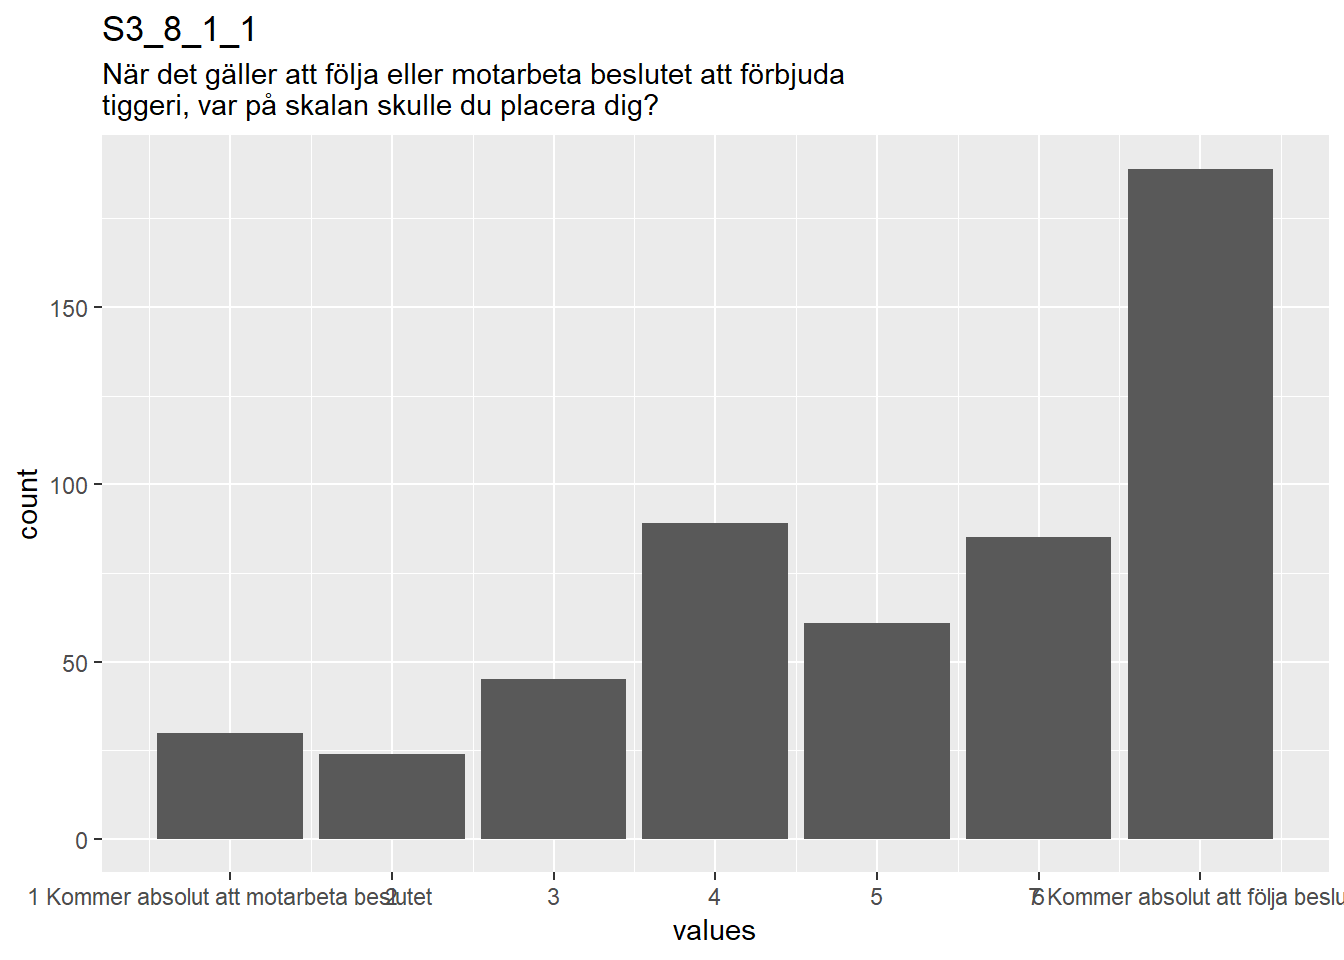
\includegraphics{Goodloser-appendix_files/figure-latex/S3_8_1_1_distribution-1.pdf}

\begin{Shaded}
\begin{Highlighting}[]
\NormalTok{knitr}\OperatorTok{::}\NormalTok{opts_chunk}\OperatorTok{$}\KeywordTok{set}\NormalTok{(}\DataTypeTok{fig.height =}\NormalTok{ old_height)}
\end{Highlighting}
\end{Shaded}

496 missings.

\subsubsection{Summary statistics}\label{S3_8_1_1_summary}

\begin{Shaded}
\begin{Highlighting}[]
\KeywordTok{attributes}\NormalTok{(item) <-}\StringTok{ }\NormalTok{item_attributes}
\NormalTok{df =}\StringTok{ }\KeywordTok{data.frame}\NormalTok{(item, }\DataTypeTok{stringsAsFactors =} \OtherTok{FALSE}\NormalTok{)}
\KeywordTok{names}\NormalTok{(df) =}\StringTok{ }\NormalTok{html_item_name}
\KeywordTok{escaped_table}\NormalTok{(}\KeywordTok{codebook_table}\NormalTok{(df))}
\end{Highlighting}
\end{Shaded}

name

label

data\_type

value\_labels

missing

complete

n

mean

sd

p0

p25

p50

p75

p100

hist

format.spss

display\_width

S3\_8\_1\_1

När det gäller att följa eller motarbeta beslutet att förbjuda tiggeri,
var på skalan skulle du placera dig?

numeric

\begin{enumerate}
\def\labelenumi{\arabic{enumi}.}
\tightlist
\item
  1 Kommer absolut att motarbeta beslutet,2. 2,3. 3,4. 4,5. 5,6. 6,7. 7
  Kommer absolut att följa beslutet

  496

  523

  1019

  5.18

  1.85

  1

  4

  6

  7

  7

  ▁▁▂▃▁▂▃▇

  F1.0

  12
\end{enumerate}

\begin{Shaded}
\begin{Highlighting}[]
\ControlFlowTok{if}\NormalTok{ (show_missings) \{}
  \KeywordTok{plot_labelled}\NormalTok{(missings, item_name, wrap_at)}
\NormalTok{\}}
\end{Highlighting}
\end{Shaded}

\begin{Shaded}
\begin{Highlighting}[]
\ControlFlowTok{if}\NormalTok{ (}\OperatorTok{!}\KeywordTok{is.null}\NormalTok{(item_info)) \{}
  \CommentTok{# don't show choices again, if they're basically same thing as value labels}
  \ControlFlowTok{if}\NormalTok{ (}\OperatorTok{!}\KeywordTok{is.null}\NormalTok{(choices) }\OperatorTok{&&}\StringTok{ }\OperatorTok{!}\KeywordTok{is.null}\NormalTok{(item_info}\OperatorTok{$}\NormalTok{choices) }\OperatorTok{&&}\StringTok{ }
\StringTok{    }\KeywordTok{all}\NormalTok{(}\KeywordTok{names}\NormalTok{(}\KeywordTok{na.omit}\NormalTok{(choices)) }\OperatorTok{==}\StringTok{ }\NormalTok{item_info}\OperatorTok{$}\NormalTok{choices) }\OperatorTok{&&}
\StringTok{    }\KeywordTok{all}\NormalTok{(}\KeywordTok{na.omit}\NormalTok{(choices) }\OperatorTok{==}\StringTok{ }\KeywordTok{names}\NormalTok{(item_info}\OperatorTok{$}\NormalTok{choices))) \{}
\NormalTok{    item_info}\OperatorTok{$}\NormalTok{choices <-}\StringTok{ }\OtherTok{NULL}
\NormalTok{  \}}
\NormalTok{  item_info}\OperatorTok{$}\NormalTok{label_parsed <-}\StringTok{ }
\StringTok{    }\NormalTok{item_info}\OperatorTok{$}\NormalTok{choice_list <-}\StringTok{ }\NormalTok{item_info}\OperatorTok{$}\NormalTok{study_id <-}\StringTok{ }\NormalTok{item_info}\OperatorTok{$}\NormalTok{id <-}\StringTok{ }\OtherTok{NULL}
\NormalTok{  pander}\OperatorTok{::}\KeywordTok{pander}\NormalTok{(item_info)}
\NormalTok{\}}
\end{Highlighting}
\end{Shaded}

\subsubsection{Value labels}\label{S3_8_1_1_labels}

\begin{Shaded}
\begin{Highlighting}[]
\ControlFlowTok{if}\NormalTok{ (}\OperatorTok{!}\KeywordTok{is.null}\NormalTok{(choices) }\OperatorTok{&&}\StringTok{ }\KeywordTok{length}\NormalTok{(choices) }\OperatorTok{&&}\StringTok{ }\KeywordTok{length}\NormalTok{(choices) }\OperatorTok{<}\StringTok{ }\DecValTok{30}\NormalTok{) \{}
\NormalTok{    pander}\OperatorTok{::}\KeywordTok{pander}\NormalTok{(}\KeywordTok{as.list}\NormalTok{(choices))}
\NormalTok{\}}
\end{Highlighting}
\end{Shaded}

\begin{itemize}
\tightlist
\item
  \textbf{1 Kommer absolut att motarbeta beslutet}: \emph{1}
\item
  \textbf{2}: \emph{2}
\item
  \textbf{3}: \emph{3}
\item
  \textbf{4}: \emph{4}
\item
  \textbf{5}: \emph{5}
\item
  \textbf{6}: \emph{6}
\item
  \textbf{7 Kommer absolut att följa beslutet}: \emph{7}
\end{itemize}

\subsection{S3\_8\_1\_2}\label{S3_8_1_2}

När det gäller att följa eller motarbeta beslutet att inte förbjuda
tiggeri, var på skalan skulle du placera dig?

\subsubsection{Distribution}\label{S3_8_1_2_distribution}

\begin{Shaded}
\begin{Highlighting}[]
\NormalTok{show_missings <-}\StringTok{ }\OtherTok{FALSE}
\ControlFlowTok{if}\NormalTok{ (}\KeywordTok{has_label}\NormalTok{(item)) \{}
\NormalTok{  missings <-}\StringTok{ }\NormalTok{item[}\KeywordTok{is.na}\NormalTok{(haven}\OperatorTok{::}\KeywordTok{zap_missing}\NormalTok{(item))]}
  \KeywordTok{attributes}\NormalTok{(missings) <-}\StringTok{ }\KeywordTok{attributes}\NormalTok{(item)}
  \ControlFlowTok{if}\NormalTok{ (}\OperatorTok{!}\KeywordTok{is.null}\NormalTok{(}\KeywordTok{attributes}\NormalTok{(item)}\OperatorTok{$}\NormalTok{labels)) \{}
    \KeywordTok{attributes}\NormalTok{(missings)}\OperatorTok{$}\NormalTok{labels <-}\StringTok{ }\KeywordTok{attributes}\NormalTok{(missings)}\OperatorTok{$}\NormalTok{labels[}\KeywordTok{is.na}\NormalTok{(}\KeywordTok{attributes}\NormalTok{(missings)}\OperatorTok{$}\NormalTok{labels)]}
    \KeywordTok{attributes}\NormalTok{(item)}\OperatorTok{$}\NormalTok{labels <-}\StringTok{ }\KeywordTok{attributes}\NormalTok{(item)}\OperatorTok{$}\NormalTok{labels[}\OperatorTok{!}\KeywordTok{is.na}\NormalTok{(}\KeywordTok{attributes}\NormalTok{(item)}\OperatorTok{$}\NormalTok{labels)]}
\NormalTok{  \}}
  \ControlFlowTok{if}\NormalTok{ (}\KeywordTok{is.numeric}\NormalTok{(item)) \{}
\NormalTok{    show_missings <-}\StringTok{ }\KeywordTok{length}\NormalTok{(}\KeywordTok{unique}\NormalTok{(haven}\OperatorTok{::}\KeywordTok{na_tag}\NormalTok{(missings))) }\OperatorTok{>}\StringTok{ }\DecValTok{1}
\NormalTok{    item <-}\StringTok{ }\NormalTok{haven}\OperatorTok{::}\KeywordTok{zap_missing}\NormalTok{(item)}
\NormalTok{  \}}
  \ControlFlowTok{if}\NormalTok{ (}\KeywordTok{length}\NormalTok{(item_attributes}\OperatorTok{$}\NormalTok{labels) }\OperatorTok{==}\StringTok{ }\DecValTok{0} \OperatorTok{&&}\StringTok{ }\KeywordTok{is.numeric}\NormalTok{(item)) \{}
\NormalTok{    item <-}\StringTok{ }\NormalTok{haven}\OperatorTok{::}\KeywordTok{zap_labels}\NormalTok{(item)}
\NormalTok{  \}}
\NormalTok{\}}
\NormalTok{item_nomiss <-}\StringTok{ }\NormalTok{item[}\OperatorTok{!}\KeywordTok{is.na}\NormalTok{(item)]}

\CommentTok{# unnest mc_multiple and so on}
\ControlFlowTok{if}\NormalTok{ (}
  \KeywordTok{is.character}\NormalTok{(item_nomiss) }\OperatorTok{&&}
\StringTok{  }\NormalTok{stringr}\OperatorTok{::}\KeywordTok{str_detect}\NormalTok{(item_nomiss, stringr}\OperatorTok{::}\KeywordTok{fixed}\NormalTok{(}\StringTok{", "}\NormalTok{)) }\OperatorTok{&&}
\StringTok{  }\NormalTok{(}\KeywordTok{exists}\NormalTok{(}\StringTok{"type"}\NormalTok{, item_info) }\OperatorTok{&&}\StringTok{ }
\StringTok{    }\NormalTok{stringr}\OperatorTok{::}\KeywordTok{str_detect}\NormalTok{(item_info}\OperatorTok{$}\NormalTok{type, }\DataTypeTok{pattern =}\NormalTok{ stringr}\OperatorTok{::}\KeywordTok{fixed}\NormalTok{(}\StringTok{"multiple"}\NormalTok{)))}
\NormalTok{  ) \{}
\NormalTok{  item_nomiss <-}\StringTok{ }\KeywordTok{unlist}\NormalTok{(stringr}\OperatorTok{::}\KeywordTok{str_split}\NormalTok{(item_nomiss, }\DataTypeTok{pattern =}\NormalTok{ stringr}\OperatorTok{::}\KeywordTok{fixed}\NormalTok{(}\StringTok{", "}\NormalTok{)))}
\NormalTok{\}}
\KeywordTok{attributes}\NormalTok{(item_nomiss) <-}\StringTok{ }\KeywordTok{attributes}\NormalTok{(item)}

\NormalTok{old_height <-}\StringTok{ }\NormalTok{knitr}\OperatorTok{::}\NormalTok{opts_chunk}\OperatorTok{$}\KeywordTok{get}\NormalTok{(}\StringTok{"fig.height"}\NormalTok{)}
\NormalTok{non_missing_choices <-}\StringTok{ }\NormalTok{item_attributes[[}\StringTok{"labels"}\NormalTok{]]}
\NormalTok{many_labels <-}\StringTok{ }\KeywordTok{length}\NormalTok{(non_missing_choices) }\OperatorTok{>}\StringTok{ }\DecValTok{7}
\NormalTok{go_vertical <-}\StringTok{ }\OperatorTok{!}\KeywordTok{is.numeric}\NormalTok{(item_nomiss) }\OperatorTok{||}\StringTok{ }\NormalTok{many_labels}
\ControlFlowTok{if}\NormalTok{ ( go_vertical ) \{}
  \CommentTok{# numeric items are plotted horizontally (because that's what usually expected)}
  \CommentTok{# categorical items are plotted vertically because we can use the screen real estate better this way}

    \ControlFlowTok{if}\NormalTok{ (}\KeywordTok{is.null}\NormalTok{(choices) }\OperatorTok{||}\StringTok{ }
\StringTok{        }\NormalTok{dplyr}\OperatorTok{::}\KeywordTok{n_distinct}\NormalTok{(item_nomiss) }\OperatorTok{>}\StringTok{ }\KeywordTok{length}\NormalTok{(non_missing_choices)) \{}
\NormalTok{        non_missing_choices <-}\StringTok{ }\KeywordTok{unique}\NormalTok{(item_nomiss)}
        \KeywordTok{names}\NormalTok{(non_missing_choices) <-}\StringTok{ }\NormalTok{non_missing_choices}
\NormalTok{    \}}
\NormalTok{  choice_multiplier <-}\StringTok{ }\NormalTok{old_height}\OperatorTok{/}\FloatTok{6.5}
\NormalTok{    new_height <-}\StringTok{ }\DecValTok{2} \OperatorTok{+}\StringTok{ }\NormalTok{choice_multiplier }\OperatorTok{*}\StringTok{ }\KeywordTok{length}\NormalTok{(non_missing_choices)}
\NormalTok{    new_height <-}\StringTok{ }\KeywordTok{ifelse}\NormalTok{(new_height }\OperatorTok{>}\StringTok{ }\DecValTok{20}\NormalTok{, }\DecValTok{20}\NormalTok{, new_height)}
\NormalTok{    new_height <-}\StringTok{ }\KeywordTok{ifelse}\NormalTok{(new_height }\OperatorTok{<}\StringTok{ }\DecValTok{1}\NormalTok{, }\DecValTok{1}\NormalTok{, new_height)}
\NormalTok{    knitr}\OperatorTok{::}\NormalTok{opts_chunk}\OperatorTok{$}\KeywordTok{set}\NormalTok{(}\DataTypeTok{fig.height =}\NormalTok{ new_height)}
\NormalTok{\}}

\NormalTok{wrap_at <-}\StringTok{ }\NormalTok{knitr}\OperatorTok{::}\NormalTok{opts_chunk}\OperatorTok{$}\KeywordTok{get}\NormalTok{(}\StringTok{"fig.width"}\NormalTok{) }\OperatorTok{*}\StringTok{ }\DecValTok{10}
\end{Highlighting}
\end{Shaded}

\begin{Shaded}
\begin{Highlighting}[]
\CommentTok{# todo: if there are free-text choices mingled in with the pre-defined ones, don't show}
\CommentTok{# todo: show rare items if they are pre-defined}
\CommentTok{# todo: bin rare responses into "other category"}
\ControlFlowTok{if}\NormalTok{ (}\OperatorTok{!}\KeywordTok{length}\NormalTok{(item_nomiss)) \{}
  \KeywordTok{cat}\NormalTok{(}\StringTok{"No non-missing values to show."}\NormalTok{)}
\NormalTok{\} }\ControlFlowTok{else} \ControlFlowTok{if}\NormalTok{ (}\KeywordTok{is.numeric}\NormalTok{(item_nomiss) }\OperatorTok{||}\StringTok{ }\NormalTok{dplyr}\OperatorTok{::}\KeywordTok{n_distinct}\NormalTok{(item_nomiss) }\OperatorTok{<}\StringTok{ }\DecValTok{20}\NormalTok{) \{}
  \KeywordTok{plot_labelled}\NormalTok{(item_nomiss, item_name, wrap_at, go_vertical)}
\NormalTok{\} }\ControlFlowTok{else}\NormalTok{ \{}
    \KeywordTok{cat}\NormalTok{(dplyr}\OperatorTok{::}\KeywordTok{n_distinct}\NormalTok{(item_nomiss), }\StringTok{" unique, categorical values, so not shown."}\NormalTok{)}
\NormalTok{\}}
\end{Highlighting}
\end{Shaded}

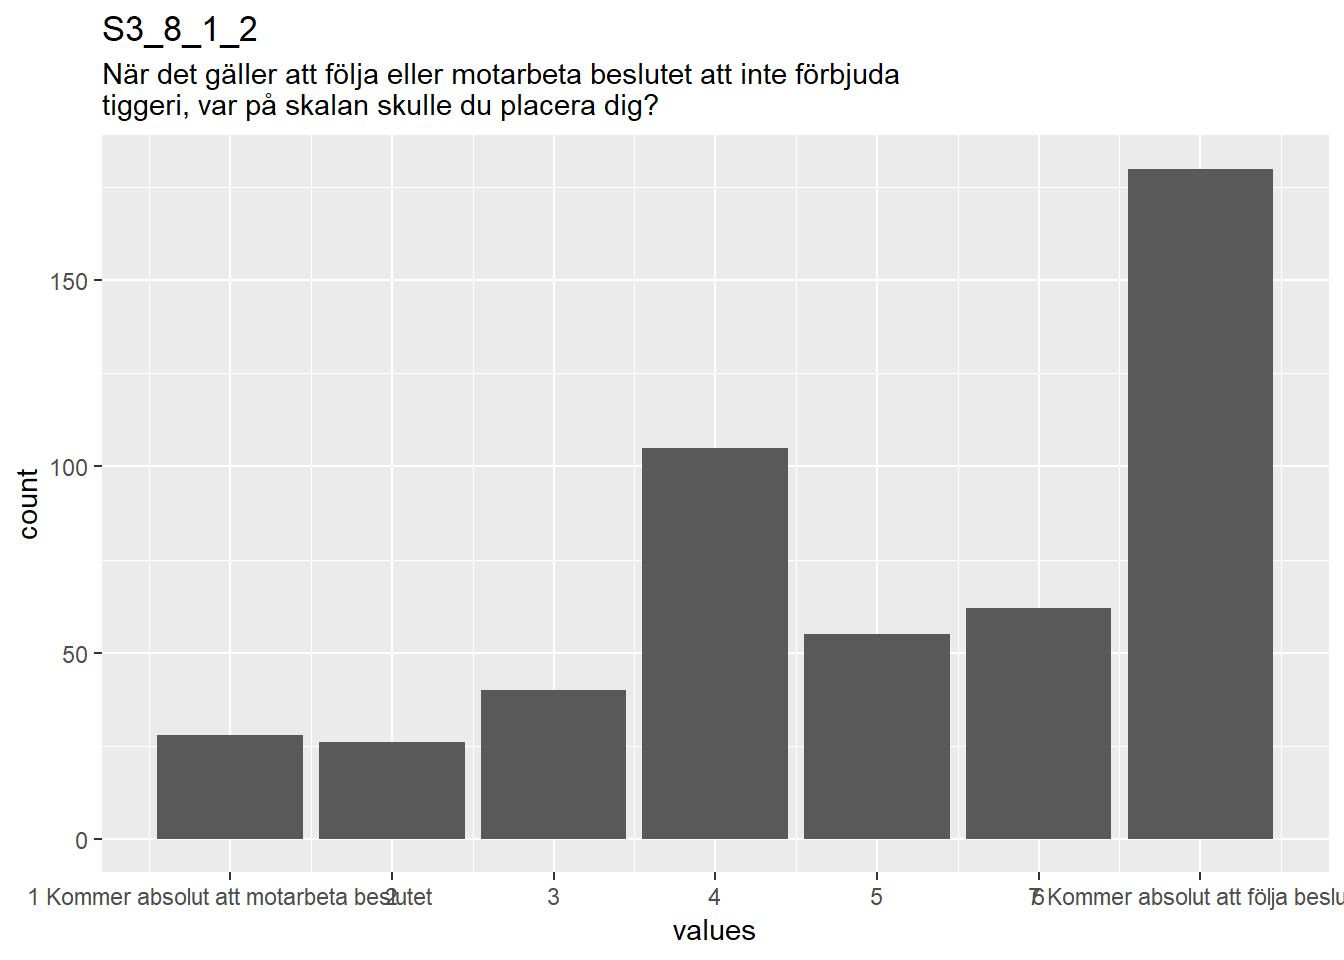
\includegraphics{Goodloser-appendix_files/figure-latex/S3_8_1_2_distribution-1.pdf}

\begin{Shaded}
\begin{Highlighting}[]
\NormalTok{knitr}\OperatorTok{::}\NormalTok{opts_chunk}\OperatorTok{$}\KeywordTok{set}\NormalTok{(}\DataTypeTok{fig.height =}\NormalTok{ old_height)}
\end{Highlighting}
\end{Shaded}

523 missings.

\subsubsection{Summary statistics}\label{S3_8_1_2_summary}

\begin{Shaded}
\begin{Highlighting}[]
\KeywordTok{attributes}\NormalTok{(item) <-}\StringTok{ }\NormalTok{item_attributes}
\NormalTok{df =}\StringTok{ }\KeywordTok{data.frame}\NormalTok{(item, }\DataTypeTok{stringsAsFactors =} \OtherTok{FALSE}\NormalTok{)}
\KeywordTok{names}\NormalTok{(df) =}\StringTok{ }\NormalTok{html_item_name}
\KeywordTok{escaped_table}\NormalTok{(}\KeywordTok{codebook_table}\NormalTok{(df))}
\end{Highlighting}
\end{Shaded}

name

label

data\_type

value\_labels

missing

complete

n

mean

sd

p0

p25

p50

p75

p100

hist

format.spss

S3\_8\_1\_2

När det gäller att följa eller motarbeta beslutet att inte förbjuda
tiggeri, var på skalan skulle du placera dig?

numeric

\begin{enumerate}
\def\labelenumi{\arabic{enumi}.}
\tightlist
\item
  1 Kommer absolut att motarbeta beslutet,2. 2,3. 3,4. 4,5. 5,6. 6,7. 7
  Kommer absolut att följa beslutet

  523

  496

  1019

  5.09

  1.87

  1

  4

  5

  7

  7

  ▁▁▂▅▁▂▃▇

  F1.0
\end{enumerate}

\begin{Shaded}
\begin{Highlighting}[]
\ControlFlowTok{if}\NormalTok{ (show_missings) \{}
  \KeywordTok{plot_labelled}\NormalTok{(missings, item_name, wrap_at)}
\NormalTok{\}}
\end{Highlighting}
\end{Shaded}

\begin{Shaded}
\begin{Highlighting}[]
\ControlFlowTok{if}\NormalTok{ (}\OperatorTok{!}\KeywordTok{is.null}\NormalTok{(item_info)) \{}
  \CommentTok{# don't show choices again, if they're basically same thing as value labels}
  \ControlFlowTok{if}\NormalTok{ (}\OperatorTok{!}\KeywordTok{is.null}\NormalTok{(choices) }\OperatorTok{&&}\StringTok{ }\OperatorTok{!}\KeywordTok{is.null}\NormalTok{(item_info}\OperatorTok{$}\NormalTok{choices) }\OperatorTok{&&}\StringTok{ }
\StringTok{    }\KeywordTok{all}\NormalTok{(}\KeywordTok{names}\NormalTok{(}\KeywordTok{na.omit}\NormalTok{(choices)) }\OperatorTok{==}\StringTok{ }\NormalTok{item_info}\OperatorTok{$}\NormalTok{choices) }\OperatorTok{&&}
\StringTok{    }\KeywordTok{all}\NormalTok{(}\KeywordTok{na.omit}\NormalTok{(choices) }\OperatorTok{==}\StringTok{ }\KeywordTok{names}\NormalTok{(item_info}\OperatorTok{$}\NormalTok{choices))) \{}
\NormalTok{    item_info}\OperatorTok{$}\NormalTok{choices <-}\StringTok{ }\OtherTok{NULL}
\NormalTok{  \}}
\NormalTok{  item_info}\OperatorTok{$}\NormalTok{label_parsed <-}\StringTok{ }
\StringTok{    }\NormalTok{item_info}\OperatorTok{$}\NormalTok{choice_list <-}\StringTok{ }\NormalTok{item_info}\OperatorTok{$}\NormalTok{study_id <-}\StringTok{ }\NormalTok{item_info}\OperatorTok{$}\NormalTok{id <-}\StringTok{ }\OtherTok{NULL}
\NormalTok{  pander}\OperatorTok{::}\KeywordTok{pander}\NormalTok{(item_info)}
\NormalTok{\}}
\end{Highlighting}
\end{Shaded}

\subsubsection{Value labels}\label{S3_8_1_2_labels}

\begin{Shaded}
\begin{Highlighting}[]
\ControlFlowTok{if}\NormalTok{ (}\OperatorTok{!}\KeywordTok{is.null}\NormalTok{(choices) }\OperatorTok{&&}\StringTok{ }\KeywordTok{length}\NormalTok{(choices) }\OperatorTok{&&}\StringTok{ }\KeywordTok{length}\NormalTok{(choices) }\OperatorTok{<}\StringTok{ }\DecValTok{30}\NormalTok{) \{}
\NormalTok{    pander}\OperatorTok{::}\KeywordTok{pander}\NormalTok{(}\KeywordTok{as.list}\NormalTok{(choices))}
\NormalTok{\}}
\end{Highlighting}
\end{Shaded}

\begin{itemize}
\tightlist
\item
  \textbf{1 Kommer absolut att motarbeta beslutet}: \emph{1}
\item
  \textbf{2}: \emph{2}
\item
  \textbf{3}: \emph{3}
\item
  \textbf{4}: \emph{4}
\item
  \textbf{5}: \emph{5}
\item
  \textbf{6}: \emph{6}
\item
  \textbf{7 Kommer absolut att följa beslutet}: \emph{7}
\end{itemize}

\subsection{Studie3sel}\label{Studie3sel}

Manipulation

\subsubsection{Distribution}\label{Studie3sel_distribution}

\begin{Shaded}
\begin{Highlighting}[]
\NormalTok{show_missings <-}\StringTok{ }\OtherTok{FALSE}
\ControlFlowTok{if}\NormalTok{ (}\KeywordTok{has_label}\NormalTok{(item)) \{}
\NormalTok{  missings <-}\StringTok{ }\NormalTok{item[}\KeywordTok{is.na}\NormalTok{(haven}\OperatorTok{::}\KeywordTok{zap_missing}\NormalTok{(item))]}
  \KeywordTok{attributes}\NormalTok{(missings) <-}\StringTok{ }\KeywordTok{attributes}\NormalTok{(item)}
  \ControlFlowTok{if}\NormalTok{ (}\OperatorTok{!}\KeywordTok{is.null}\NormalTok{(}\KeywordTok{attributes}\NormalTok{(item)}\OperatorTok{$}\NormalTok{labels)) \{}
    \KeywordTok{attributes}\NormalTok{(missings)}\OperatorTok{$}\NormalTok{labels <-}\StringTok{ }\KeywordTok{attributes}\NormalTok{(missings)}\OperatorTok{$}\NormalTok{labels[}\KeywordTok{is.na}\NormalTok{(}\KeywordTok{attributes}\NormalTok{(missings)}\OperatorTok{$}\NormalTok{labels)]}
    \KeywordTok{attributes}\NormalTok{(item)}\OperatorTok{$}\NormalTok{labels <-}\StringTok{ }\KeywordTok{attributes}\NormalTok{(item)}\OperatorTok{$}\NormalTok{labels[}\OperatorTok{!}\KeywordTok{is.na}\NormalTok{(}\KeywordTok{attributes}\NormalTok{(item)}\OperatorTok{$}\NormalTok{labels)]}
\NormalTok{  \}}
  \ControlFlowTok{if}\NormalTok{ (}\KeywordTok{is.numeric}\NormalTok{(item)) \{}
\NormalTok{    show_missings <-}\StringTok{ }\KeywordTok{length}\NormalTok{(}\KeywordTok{unique}\NormalTok{(haven}\OperatorTok{::}\KeywordTok{na_tag}\NormalTok{(missings))) }\OperatorTok{>}\StringTok{ }\DecValTok{1}
\NormalTok{    item <-}\StringTok{ }\NormalTok{haven}\OperatorTok{::}\KeywordTok{zap_missing}\NormalTok{(item)}
\NormalTok{  \}}
  \ControlFlowTok{if}\NormalTok{ (}\KeywordTok{length}\NormalTok{(item_attributes}\OperatorTok{$}\NormalTok{labels) }\OperatorTok{==}\StringTok{ }\DecValTok{0} \OperatorTok{&&}\StringTok{ }\KeywordTok{is.numeric}\NormalTok{(item)) \{}
\NormalTok{    item <-}\StringTok{ }\NormalTok{haven}\OperatorTok{::}\KeywordTok{zap_labels}\NormalTok{(item)}
\NormalTok{  \}}
\NormalTok{\}}
\NormalTok{item_nomiss <-}\StringTok{ }\NormalTok{item[}\OperatorTok{!}\KeywordTok{is.na}\NormalTok{(item)]}

\CommentTok{# unnest mc_multiple and so on}
\ControlFlowTok{if}\NormalTok{ (}
  \KeywordTok{is.character}\NormalTok{(item_nomiss) }\OperatorTok{&&}
\StringTok{  }\NormalTok{stringr}\OperatorTok{::}\KeywordTok{str_detect}\NormalTok{(item_nomiss, stringr}\OperatorTok{::}\KeywordTok{fixed}\NormalTok{(}\StringTok{", "}\NormalTok{)) }\OperatorTok{&&}
\StringTok{  }\NormalTok{(}\KeywordTok{exists}\NormalTok{(}\StringTok{"type"}\NormalTok{, item_info) }\OperatorTok{&&}\StringTok{ }
\StringTok{    }\NormalTok{stringr}\OperatorTok{::}\KeywordTok{str_detect}\NormalTok{(item_info}\OperatorTok{$}\NormalTok{type, }\DataTypeTok{pattern =}\NormalTok{ stringr}\OperatorTok{::}\KeywordTok{fixed}\NormalTok{(}\StringTok{"multiple"}\NormalTok{)))}
\NormalTok{  ) \{}
\NormalTok{  item_nomiss <-}\StringTok{ }\KeywordTok{unlist}\NormalTok{(stringr}\OperatorTok{::}\KeywordTok{str_split}\NormalTok{(item_nomiss, }\DataTypeTok{pattern =}\NormalTok{ stringr}\OperatorTok{::}\KeywordTok{fixed}\NormalTok{(}\StringTok{", "}\NormalTok{)))}
\NormalTok{\}}
\KeywordTok{attributes}\NormalTok{(item_nomiss) <-}\StringTok{ }\KeywordTok{attributes}\NormalTok{(item)}

\NormalTok{old_height <-}\StringTok{ }\NormalTok{knitr}\OperatorTok{::}\NormalTok{opts_chunk}\OperatorTok{$}\KeywordTok{get}\NormalTok{(}\StringTok{"fig.height"}\NormalTok{)}
\NormalTok{non_missing_choices <-}\StringTok{ }\NormalTok{item_attributes[[}\StringTok{"labels"}\NormalTok{]]}
\NormalTok{many_labels <-}\StringTok{ }\KeywordTok{length}\NormalTok{(non_missing_choices) }\OperatorTok{>}\StringTok{ }\DecValTok{7}
\NormalTok{go_vertical <-}\StringTok{ }\OperatorTok{!}\KeywordTok{is.numeric}\NormalTok{(item_nomiss) }\OperatorTok{||}\StringTok{ }\NormalTok{many_labels}
\ControlFlowTok{if}\NormalTok{ ( go_vertical ) \{}
  \CommentTok{# numeric items are plotted horizontally (because that's what usually expected)}
  \CommentTok{# categorical items are plotted vertically because we can use the screen real estate better this way}

    \ControlFlowTok{if}\NormalTok{ (}\KeywordTok{is.null}\NormalTok{(choices) }\OperatorTok{||}\StringTok{ }
\StringTok{        }\NormalTok{dplyr}\OperatorTok{::}\KeywordTok{n_distinct}\NormalTok{(item_nomiss) }\OperatorTok{>}\StringTok{ }\KeywordTok{length}\NormalTok{(non_missing_choices)) \{}
\NormalTok{        non_missing_choices <-}\StringTok{ }\KeywordTok{unique}\NormalTok{(item_nomiss)}
        \KeywordTok{names}\NormalTok{(non_missing_choices) <-}\StringTok{ }\NormalTok{non_missing_choices}
\NormalTok{    \}}
\NormalTok{  choice_multiplier <-}\StringTok{ }\NormalTok{old_height}\OperatorTok{/}\FloatTok{6.5}
\NormalTok{    new_height <-}\StringTok{ }\DecValTok{2} \OperatorTok{+}\StringTok{ }\NormalTok{choice_multiplier }\OperatorTok{*}\StringTok{ }\KeywordTok{length}\NormalTok{(non_missing_choices)}
\NormalTok{    new_height <-}\StringTok{ }\KeywordTok{ifelse}\NormalTok{(new_height }\OperatorTok{>}\StringTok{ }\DecValTok{20}\NormalTok{, }\DecValTok{20}\NormalTok{, new_height)}
\NormalTok{    new_height <-}\StringTok{ }\KeywordTok{ifelse}\NormalTok{(new_height }\OperatorTok{<}\StringTok{ }\DecValTok{1}\NormalTok{, }\DecValTok{1}\NormalTok{, new_height)}
\NormalTok{    knitr}\OperatorTok{::}\NormalTok{opts_chunk}\OperatorTok{$}\KeywordTok{set}\NormalTok{(}\DataTypeTok{fig.height =}\NormalTok{ new_height)}
\NormalTok{\}}

\NormalTok{wrap_at <-}\StringTok{ }\NormalTok{knitr}\OperatorTok{::}\NormalTok{opts_chunk}\OperatorTok{$}\KeywordTok{get}\NormalTok{(}\StringTok{"fig.width"}\NormalTok{) }\OperatorTok{*}\StringTok{ }\DecValTok{10}
\end{Highlighting}
\end{Shaded}

\begin{Shaded}
\begin{Highlighting}[]
\CommentTok{# todo: if there are free-text choices mingled in with the pre-defined ones, don't show}
\CommentTok{# todo: show rare items if they are pre-defined}
\CommentTok{# todo: bin rare responses into "other category"}
\ControlFlowTok{if}\NormalTok{ (}\OperatorTok{!}\KeywordTok{length}\NormalTok{(item_nomiss)) \{}
  \KeywordTok{cat}\NormalTok{(}\StringTok{"No non-missing values to show."}\NormalTok{)}
\NormalTok{\} }\ControlFlowTok{else} \ControlFlowTok{if}\NormalTok{ (}\KeywordTok{is.numeric}\NormalTok{(item_nomiss) }\OperatorTok{||}\StringTok{ }\NormalTok{dplyr}\OperatorTok{::}\KeywordTok{n_distinct}\NormalTok{(item_nomiss) }\OperatorTok{<}\StringTok{ }\DecValTok{20}\NormalTok{) \{}
  \KeywordTok{plot_labelled}\NormalTok{(item_nomiss, item_name, wrap_at, go_vertical)}
\NormalTok{\} }\ControlFlowTok{else}\NormalTok{ \{}
    \KeywordTok{cat}\NormalTok{(dplyr}\OperatorTok{::}\KeywordTok{n_distinct}\NormalTok{(item_nomiss), }\StringTok{" unique, categorical values, so not shown."}\NormalTok{)}
\NormalTok{\}}
\end{Highlighting}
\end{Shaded}

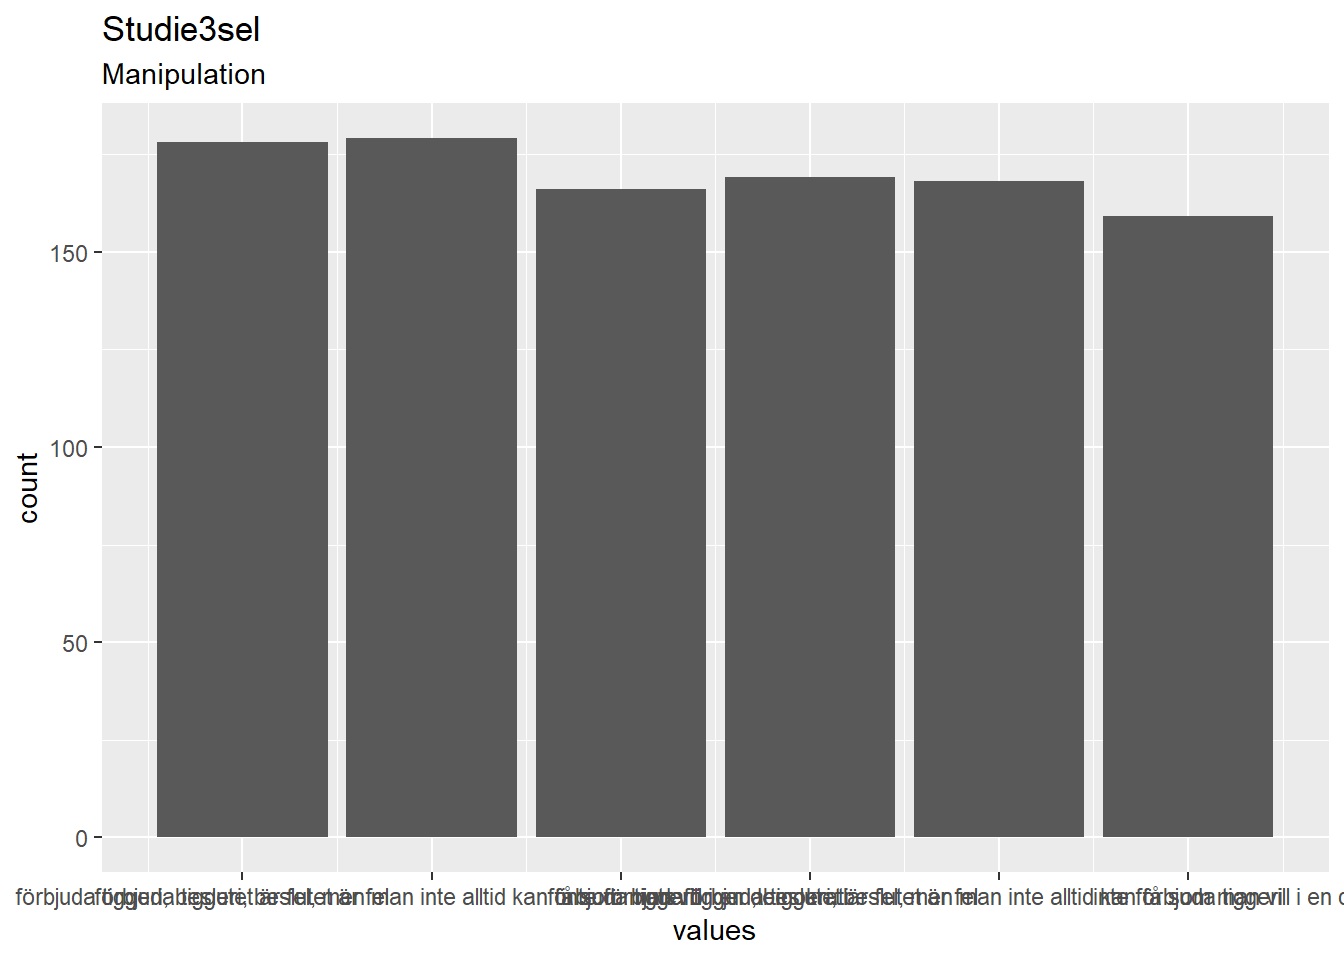
\includegraphics{Goodloser-appendix_files/figure-latex/Studie3sel_distribution-1.pdf}

\begin{Shaded}
\begin{Highlighting}[]
\NormalTok{knitr}\OperatorTok{::}\NormalTok{opts_chunk}\OperatorTok{$}\KeywordTok{set}\NormalTok{(}\DataTypeTok{fig.height =}\NormalTok{ old_height)}
\end{Highlighting}
\end{Shaded}

0 missings.

\subsubsection{Summary statistics}\label{Studie3sel_summary}

\begin{Shaded}
\begin{Highlighting}[]
\KeywordTok{attributes}\NormalTok{(item) <-}\StringTok{ }\NormalTok{item_attributes}
\NormalTok{df =}\StringTok{ }\KeywordTok{data.frame}\NormalTok{(item, }\DataTypeTok{stringsAsFactors =} \OtherTok{FALSE}\NormalTok{)}
\KeywordTok{names}\NormalTok{(df) =}\StringTok{ }\NormalTok{html_item_name}
\KeywordTok{escaped_table}\NormalTok{(}\KeywordTok{codebook_table}\NormalTok{(df))}
\end{Highlighting}
\end{Shaded}

name

label

data\_type

value\_labels

missing

complete

n

mean

sd

p0

p25

p50

p75

p100

hist

format.spss

display\_width

Studie3sel

Manipulation

numeric

\begin{enumerate}
\def\labelenumi{\arabic{enumi}.}
\tightlist
\item
  förbjuda tiggeri, beslutet är fel,2. förbjuda tiggeri, beslutet är
  fel, men man inte alltid kan få som man vill i en demokrati,3.
  förbjuda tiggeri,4. inte förbjuda tiggeri, beslutet är fel,5. inte
  förbjuda tiggeri, beslutet är fel, men man inte alltid kan få som man
  vill i en demokrati,6. inte förbjuda tiggeri

  0

  1019

  1019

  3.44

  1.71

  1

  2

  3

  5

  6

  ▇▇▁▇▇▁▇▇

  F1.0

  12
\end{enumerate}

\begin{Shaded}
\begin{Highlighting}[]
\ControlFlowTok{if}\NormalTok{ (show_missings) \{}
  \KeywordTok{plot_labelled}\NormalTok{(missings, item_name, wrap_at)}
\NormalTok{\}}
\end{Highlighting}
\end{Shaded}

\begin{Shaded}
\begin{Highlighting}[]
\ControlFlowTok{if}\NormalTok{ (}\OperatorTok{!}\KeywordTok{is.null}\NormalTok{(item_info)) \{}
  \CommentTok{# don't show choices again, if they're basically same thing as value labels}
  \ControlFlowTok{if}\NormalTok{ (}\OperatorTok{!}\KeywordTok{is.null}\NormalTok{(choices) }\OperatorTok{&&}\StringTok{ }\OperatorTok{!}\KeywordTok{is.null}\NormalTok{(item_info}\OperatorTok{$}\NormalTok{choices) }\OperatorTok{&&}\StringTok{ }
\StringTok{    }\KeywordTok{all}\NormalTok{(}\KeywordTok{names}\NormalTok{(}\KeywordTok{na.omit}\NormalTok{(choices)) }\OperatorTok{==}\StringTok{ }\NormalTok{item_info}\OperatorTok{$}\NormalTok{choices) }\OperatorTok{&&}
\StringTok{    }\KeywordTok{all}\NormalTok{(}\KeywordTok{na.omit}\NormalTok{(choices) }\OperatorTok{==}\StringTok{ }\KeywordTok{names}\NormalTok{(item_info}\OperatorTok{$}\NormalTok{choices))) \{}
\NormalTok{    item_info}\OperatorTok{$}\NormalTok{choices <-}\StringTok{ }\OtherTok{NULL}
\NormalTok{  \}}
\NormalTok{  item_info}\OperatorTok{$}\NormalTok{label_parsed <-}\StringTok{ }
\StringTok{    }\NormalTok{item_info}\OperatorTok{$}\NormalTok{choice_list <-}\StringTok{ }\NormalTok{item_info}\OperatorTok{$}\NormalTok{study_id <-}\StringTok{ }\NormalTok{item_info}\OperatorTok{$}\NormalTok{id <-}\StringTok{ }\OtherTok{NULL}
\NormalTok{  pander}\OperatorTok{::}\KeywordTok{pander}\NormalTok{(item_info)}
\NormalTok{\}}
\end{Highlighting}
\end{Shaded}

\subsubsection{Value labels}\label{Studie3sel_labels}

\begin{Shaded}
\begin{Highlighting}[]
\ControlFlowTok{if}\NormalTok{ (}\OperatorTok{!}\KeywordTok{is.null}\NormalTok{(choices) }\OperatorTok{&&}\StringTok{ }\KeywordTok{length}\NormalTok{(choices) }\OperatorTok{&&}\StringTok{ }\KeywordTok{length}\NormalTok{(choices) }\OperatorTok{<}\StringTok{ }\DecValTok{30}\NormalTok{) \{}
\NormalTok{    pander}\OperatorTok{::}\KeywordTok{pander}\NormalTok{(}\KeywordTok{as.list}\NormalTok{(choices))}
\NormalTok{\}}
\end{Highlighting}
\end{Shaded}

\begin{itemize}
\tightlist
\item
  \textbf{förbjuda tiggeri, beslutet är fel}: \emph{1}
\item
  \textbf{förbjuda tiggeri, beslutet är fel, men man inte alltid kan få
  som man vill i en demokrati}: \emph{2}
\item
  \textbf{förbjuda tiggeri}: \emph{3}
\item
  \textbf{inte förbjuda tiggeri, beslutet är fel}: \emph{4}
\item
  \textbf{inte förbjuda tiggeri, beslutet är fel, men man inte alltid
  kan få som man vill i en demokrati}: \emph{5}
\item
  \textbf{inte förbjuda tiggeri}: \emph{6}
\end{itemize}

\begin{Shaded}
\begin{Highlighting}[]
\NormalTok{missingness_report}
\end{Highlighting}
\end{Shaded}

\section{Missingness report}\label{missingness-report}

Among those who finished the survey. Only variables that have missings
are shown.

\begin{Shaded}
\begin{Highlighting}[]
\ControlFlowTok{if}\NormalTok{ (  }\KeywordTok{exists}\NormalTok{(}\StringTok{"ended"}\NormalTok{, results) }\OperatorTok{&&}
\StringTok{  }\KeywordTok{exists}\NormalTok{(}\StringTok{"expired"}\NormalTok{, results)) \{}
\NormalTok{  finisher_results <-}\StringTok{ }\NormalTok{dplyr}\OperatorTok{::}\KeywordTok{filter}\NormalTok{(results, }\OperatorTok{!}\KeywordTok{is.na}\NormalTok{(.data}\OperatorTok{$}\NormalTok{ended))}
\NormalTok{\} }\ControlFlowTok{else}\NormalTok{ \{}
\NormalTok{  finisher_results <-}\StringTok{ }\NormalTok{results}
  \KeywordTok{warning}\NormalTok{(}\StringTok{"Could not figure out who finished the surveys, because the "}\NormalTok{,}
          \StringTok{"variables expired and ended were missing."}\NormalTok{)}
\NormalTok{\}}
\end{Highlighting}
\end{Shaded}

\begin{verbatim}
## Warning: Could not figure out who finished the surveys, because the
## variables expired and ended were missing.
\end{verbatim}

\begin{Shaded}
\begin{Highlighting}[]
\ControlFlowTok{if}\NormalTok{ (}\KeywordTok{length}\NormalTok{(md_pattern)) \{}
\NormalTok{  pander}\OperatorTok{::}\KeywordTok{pander}\NormalTok{(md_pattern)}
\NormalTok{\}}
\end{Highlighting}
\end{Shaded}

\begin{longtable}[]{@{}cccccc@{}}
\caption{Table continues below}\tabularnewline
\toprule
\begin{minipage}[b]{0.28\columnwidth}\centering\strut
description\strut
\end{minipage} & \begin{minipage}[b]{0.07\columnwidth}\centering\strut
Q64\strut
\end{minipage} & \begin{minipage}[b]{0.12\columnwidth}\centering\strut
S3\_4\_1\_1\strut
\end{minipage} & \begin{minipage}[b]{0.12\columnwidth}\centering\strut
S3\_6\_1\_1\strut
\end{minipage} & \begin{minipage}[b]{0.12\columnwidth}\centering\strut
S3\_7\_1\_1\strut
\end{minipage} & \begin{minipage}[b]{0.12\columnwidth}\centering\strut
S3\_8\_1\_1\strut
\end{minipage}\tabularnewline
\midrule
\endfirsthead
\toprule
\begin{minipage}[b]{0.28\columnwidth}\centering\strut
description\strut
\end{minipage} & \begin{minipage}[b]{0.07\columnwidth}\centering\strut
Q64\strut
\end{minipage} & \begin{minipage}[b]{0.12\columnwidth}\centering\strut
S3\_4\_1\_1\strut
\end{minipage} & \begin{minipage}[b]{0.12\columnwidth}\centering\strut
S3\_6\_1\_1\strut
\end{minipage} & \begin{minipage}[b]{0.12\columnwidth}\centering\strut
S3\_7\_1\_1\strut
\end{minipage} & \begin{minipage}[b]{0.12\columnwidth}\centering\strut
S3\_8\_1\_1\strut
\end{minipage}\tabularnewline
\midrule
\endhead
\begin{minipage}[t]{0.28\columnwidth}\centering\strut
Missings per variable\strut
\end{minipage} & \begin{minipage}[t]{0.07\columnwidth}\centering\strut
4\strut
\end{minipage} & \begin{minipage}[t]{0.12\columnwidth}\centering\strut
496\strut
\end{minipage} & \begin{minipage}[t]{0.12\columnwidth}\centering\strut
496\strut
\end{minipage} & \begin{minipage}[t]{0.12\columnwidth}\centering\strut
496\strut
\end{minipage} & \begin{minipage}[t]{0.12\columnwidth}\centering\strut
496\strut
\end{minipage}\tabularnewline
\begin{minipage}[t]{0.28\columnwidth}\centering\strut
Missings in 4 variables\strut
\end{minipage} & \begin{minipage}[t]{0.07\columnwidth}\centering\strut
1\strut
\end{minipage} & \begin{minipage}[t]{0.12\columnwidth}\centering\strut
1\strut
\end{minipage} & \begin{minipage}[t]{0.12\columnwidth}\centering\strut
1\strut
\end{minipage} & \begin{minipage}[t]{0.12\columnwidth}\centering\strut
1\strut
\end{minipage} & \begin{minipage}[t]{0.12\columnwidth}\centering\strut
1\strut
\end{minipage}\tabularnewline
\begin{minipage}[t]{0.28\columnwidth}\centering\strut
Missings in 4 variables\strut
\end{minipage} & \begin{minipage}[t]{0.07\columnwidth}\centering\strut
1\strut
\end{minipage} & \begin{minipage}[t]{0.12\columnwidth}\centering\strut
0\strut
\end{minipage} & \begin{minipage}[t]{0.12\columnwidth}\centering\strut
0\strut
\end{minipage} & \begin{minipage}[t]{0.12\columnwidth}\centering\strut
0\strut
\end{minipage} & \begin{minipage}[t]{0.12\columnwidth}\centering\strut
0\strut
\end{minipage}\tabularnewline
\begin{minipage}[t]{0.28\columnwidth}\centering\strut
2 other, less frequent patterns\strut
\end{minipage} & \begin{minipage}[t]{0.07\columnwidth}\centering\strut
0\strut
\end{minipage} & \begin{minipage}[t]{0.12\columnwidth}\centering\strut
1\strut
\end{minipage} & \begin{minipage}[t]{0.12\columnwidth}\centering\strut
1\strut
\end{minipage} & \begin{minipage}[t]{0.12\columnwidth}\centering\strut
1\strut
\end{minipage} & \begin{minipage}[t]{0.12\columnwidth}\centering\strut
1\strut
\end{minipage}\tabularnewline
\bottomrule
\end{longtable}

\begin{longtable}[]{@{}cccccc@{}}
\toprule
\begin{minipage}[b]{0.13\columnwidth}\centering\strut
S3\_4\_1\_2\strut
\end{minipage} & \begin{minipage}[b]{0.13\columnwidth}\centering\strut
S3\_6\_1\_2\strut
\end{minipage} & \begin{minipage}[b]{0.13\columnwidth}\centering\strut
S3\_7\_1\_2\strut
\end{minipage} & \begin{minipage}[b]{0.13\columnwidth}\centering\strut
S3\_8\_1\_2\strut
\end{minipage} & \begin{minipage}[b]{0.13\columnwidth}\centering\strut
var\_miss\strut
\end{minipage} & \begin{minipage}[b]{0.09\columnwidth}\centering\strut
n\_miss\strut
\end{minipage}\tabularnewline
\midrule
\endhead
\begin{minipage}[t]{0.13\columnwidth}\centering\strut
523\strut
\end{minipage} & \begin{minipage}[t]{0.13\columnwidth}\centering\strut
523\strut
\end{minipage} & \begin{minipage}[t]{0.13\columnwidth}\centering\strut
523\strut
\end{minipage} & \begin{minipage}[t]{0.13\columnwidth}\centering\strut
523\strut
\end{minipage} & \begin{minipage}[t]{0.13\columnwidth}\centering\strut
4080\strut
\end{minipage} & \begin{minipage}[t]{0.09\columnwidth}\centering\strut
4080\strut
\end{minipage}\tabularnewline
\begin{minipage}[t]{0.13\columnwidth}\centering\strut
0\strut
\end{minipage} & \begin{minipage}[t]{0.13\columnwidth}\centering\strut
0\strut
\end{minipage} & \begin{minipage}[t]{0.13\columnwidth}\centering\strut
0\strut
\end{minipage} & \begin{minipage}[t]{0.13\columnwidth}\centering\strut
0\strut
\end{minipage} & \begin{minipage}[t]{0.13\columnwidth}\centering\strut
4\strut
\end{minipage} & \begin{minipage}[t]{0.09\columnwidth}\centering\strut
522\strut
\end{minipage}\tabularnewline
\begin{minipage}[t]{0.13\columnwidth}\centering\strut
1\strut
\end{minipage} & \begin{minipage}[t]{0.13\columnwidth}\centering\strut
1\strut
\end{minipage} & \begin{minipage}[t]{0.13\columnwidth}\centering\strut
1\strut
\end{minipage} & \begin{minipage}[t]{0.13\columnwidth}\centering\strut
1\strut
\end{minipage} & \begin{minipage}[t]{0.13\columnwidth}\centering\strut
4\strut
\end{minipage} & \begin{minipage}[t]{0.09\columnwidth}\centering\strut
493\strut
\end{minipage}\tabularnewline
\begin{minipage}[t]{0.13\columnwidth}\centering\strut
1\strut
\end{minipage} & \begin{minipage}[t]{0.13\columnwidth}\centering\strut
1\strut
\end{minipage} & \begin{minipage}[t]{0.13\columnwidth}\centering\strut
1\strut
\end{minipage} & \begin{minipage}[t]{0.13\columnwidth}\centering\strut
1\strut
\end{minipage} & \begin{minipage}[t]{0.13\columnwidth}\centering\strut
10\strut
\end{minipage} & \begin{minipage}[t]{0.09\columnwidth}\centering\strut
4\strut
\end{minipage}\tabularnewline
\bottomrule
\end{longtable}

\begin{Shaded}
\begin{Highlighting}[]
\NormalTok{items}
\end{Highlighting}
\end{Shaded}

\section{Codebook table}\label{codebook-table}

\begin{Shaded}
\begin{Highlighting}[]
\KeywordTok{export_table}\NormalTok{(metadata_table)}
\end{Highlighting}
\end{Shaded}

\begin{verbatim}
## PhantomJS not found. You can install it with webshot::install_phantomjs(). If it is installed, please make sure the phantomjs executable can be found via the PATH variable.
\end{verbatim}

\hypertarget{htmlwidget-74fe228e2c8a87a93948}{}

\begin{Shaded}
\begin{Highlighting}[]
\NormalTok{jsonld}
\end{Highlighting}
\end{Shaded}

\chapter{Data management}\label{data-management}

\begin{quote}
This chapter describes the data management that is conducted prior to
any analysis.
\end{quote}

\begin{Shaded}
\begin{Highlighting}[]
\ControlFlowTok{if}\NormalTok{(}\OperatorTok{!}\KeywordTok{require}\NormalTok{(}\StringTok{"haven"}\NormalTok{))\{}\KeywordTok{install.packages}\NormalTok{(}\StringTok{"haven"}\NormalTok{);  }\KeywordTok{library}\NormalTok{(haven)\}}
\ControlFlowTok{if}\NormalTok{(}\OperatorTok{!}\KeywordTok{require}\NormalTok{(}\StringTok{"knitr"}\NormalTok{))\{}\KeywordTok{install.packages}\NormalTok{(}\StringTok{"knitr"}\NormalTok{);  }\KeywordTok{library}\NormalTok{(knitr)\}}
\ControlFlowTok{if}\NormalTok{(}\OperatorTok{!}\KeywordTok{require}\NormalTok{(}\StringTok{"naniar"}\NormalTok{))\{}\KeywordTok{install.packages}\NormalTok{(}\StringTok{"naniar"}\NormalTok{);  }\KeywordTok{library}\NormalTok{(naniar)\}}
\ControlFlowTok{if}\NormalTok{(}\OperatorTok{!}\KeywordTok{require}\NormalTok{(}\StringTok{"tidyverse"}\NormalTok{))\{}\KeywordTok{install.packages}\NormalTok{(}\StringTok{"tidyverse"}\NormalTok{);  }\KeywordTok{library}\NormalTok{(tidyverse)\}}

\NormalTok{d <-}\StringTok{ }\KeywordTok{read_sav}\NormalTok{(}\StringTok{"C:}\CharTok{\textbackslash{}\textbackslash{}}\StringTok{Users/Sveinung/OneDrive/NORCE 2018-/goodloser/Conjoint/Bookdown-goodloser/Data/Goodloser-exp1.sav"}\NormalTok{)}

\NormalTok{knitr}\OperatorTok{::}\NormalTok{opts_chunk}\OperatorTok{$}\KeywordTok{set}\NormalTok{(}\DataTypeTok{echo =} \OtherTok{TRUE}\NormalTok{, }\DataTypeTok{knitr.kable.NA =} \StringTok{""}\NormalTok{, }\DataTypeTok{cache =} \OtherTok{FALSE}\NormalTok{, }\DataTypeTok{warning =} \OtherTok{FALSE}\NormalTok{)}
\end{Highlighting}
\end{Shaded}

\begin{Shaded}
\begin{Highlighting}[]
\NormalTok{d <-}\StringTok{ }\NormalTok{d }\OperatorTok
\StringTok{  }\KeywordTok{rename}\NormalTok{(}\StringTok{"age"}\NormalTok{ =}\StringTok{ "Q64"}\NormalTok{,}
          \StringTok{"gender"}\NormalTok{ =}\StringTok{ "Q63"}\NormalTok{,}
          \StringTok{"opinion_ban"}\NormalTok{ =}\StringTok{ "S3_1_1"}\NormalTok{,}
          \StringTok{"opinion_strength"}\NormalTok{ =}\StringTok{ "S3_2_1"}\NormalTok{,}
          \StringTok{"fairness_1"}\NormalTok{ =}\StringTok{ "S3_4_1_1"}\NormalTok{,}
          \StringTok{"fairness_2"}\NormalTok{ =}\StringTok{ "S3_4_1_2"}\NormalTok{,}
          \StringTok{"justice"}\NormalTok{ =}\StringTok{ "S3_5_1"}\NormalTok{, }\CommentTok{#Note: There was only variable with this question item}
          \StringTok{"eval_1"}\NormalTok{ =}\StringTok{ "S3_6_1_1"}\NormalTok{,}
          \StringTok{"eval_2"}\NormalTok{ =}\StringTok{ "S3_6_1_2"}\NormalTok{,}
          \StringTok{"accept_1"}\NormalTok{ =}\StringTok{ "S3_7_1_1"}\NormalTok{,}
          \StringTok{"accept_2"}\NormalTok{ =}\StringTok{ "S3_7_1_2"}\NormalTok{,}
          \StringTok{"comply_1"}\NormalTok{ =}\StringTok{ "S3_8_1_1"}\NormalTok{,}
          \StringTok{"comply_2"}\NormalTok{ =}\StringTok{ "S3_8_1_2"}\NormalTok{,}
          \StringTok{"treatment"}\NormalTok{ =}\StringTok{ "Studie3sel"}
\NormalTok{                  )}

\NormalTok{d <-}\StringTok{ }\NormalTok{d }\OperatorTok
\StringTok{  }\KeywordTok{gather}\NormalTok{(orig, fairness, fairness_}\DecValTok{1}\OperatorTok{:}\NormalTok{fairness_}\DecValTok{2}\NormalTok{) }\OperatorTok\StringTok{ }
\StringTok{  }\KeywordTok{filter}\NormalTok{(}\OperatorTok{!}\KeywordTok{is.na}\NormalTok{(fairness)) }\OperatorTok\StringTok{ }
\StringTok{  }\KeywordTok{gather}\NormalTok{(orig, eval, eval_}\DecValTok{1}\OperatorTok{:}\NormalTok{eval_}\DecValTok{2}\NormalTok{) }\OperatorTok\StringTok{ }
\StringTok{  }\KeywordTok{filter}\NormalTok{(}\OperatorTok{!}\KeywordTok{is.na}\NormalTok{(eval)) }\OperatorTok\StringTok{ }
\StringTok{  }\KeywordTok{select}\NormalTok{(}\OperatorTok{-}\NormalTok{orig) }\OperatorTok\StringTok{ }
\StringTok{  }\KeywordTok{gather}\NormalTok{(orig, accept, accept_}\DecValTok{1}\OperatorTok{:}\NormalTok{accept_}\DecValTok{2}\NormalTok{) }\OperatorTok\StringTok{ }
\StringTok{  }\KeywordTok{filter}\NormalTok{(}\OperatorTok{!}\KeywordTok{is.na}\NormalTok{(accept)) }\OperatorTok\StringTok{ }
\StringTok{  }\KeywordTok{select}\NormalTok{(}\OperatorTok{-}\NormalTok{orig) }\OperatorTok\StringTok{ }
\StringTok{  }\KeywordTok{gather}\NormalTok{(orig, comply, comply_}\DecValTok{1}\OperatorTok{:}\NormalTok{comply_}\DecValTok{2}\NormalTok{) }\OperatorTok\StringTok{ }
\StringTok{  }\KeywordTok{filter}\NormalTok{(}\OperatorTok{!}\KeywordTok{is.na}\NormalTok{(comply)) }\OperatorTok\StringTok{ }
\StringTok{  }\KeywordTok{select}\NormalTok{(}\OperatorTok{-}\NormalTok{orig) }


\NormalTok{##Create manipulation check variable that measures whether the respondents correctly identify whether the outcome was favorable or unfavorable to them}
\NormalTok{d <-}\StringTok{ }\NormalTok{d }\OperatorTok
\StringTok{  }\KeywordTok{mutate}\NormalTok{(}\DataTypeTok{favorability =} \KeywordTok{case_when}\NormalTok{(}
\NormalTok{    treatment }\OperatorTok\StringTok{ }\DecValTok{1}\OperatorTok{:}\DecValTok{3} \OperatorTok{&}\StringTok{ }\NormalTok{opinion_ban }\OperatorTok{==}\StringTok{ }\DecValTok{1} \OperatorTok{~}\StringTok{ "Unfavorable"}\NormalTok{,}
\NormalTok{    treatment }\OperatorTok\StringTok{ }\DecValTok{1}\OperatorTok{:}\DecValTok{3} \OperatorTok{&}\StringTok{ }\NormalTok{opinion_ban }\OperatorTok{==}\StringTok{ }\DecValTok{2} \OperatorTok{~}\StringTok{ "Favorable"}\NormalTok{,}
\NormalTok{    treatment }\OperatorTok\StringTok{ }\DecValTok{4}\OperatorTok{:}\DecValTok{6} \OperatorTok{&}\StringTok{ }\NormalTok{opinion_ban }\OperatorTok{==}\StringTok{ }\DecValTok{1} \OperatorTok{~}\StringTok{ "Unfavorable"}\NormalTok{,}
\NormalTok{    treatment }\OperatorTok\StringTok{ }\DecValTok{4}\OperatorTok{:}\DecValTok{6} \OperatorTok{&}\StringTok{ }\NormalTok{opinion_ban }\OperatorTok{==}\StringTok{ }\DecValTok{2} \OperatorTok{~}\StringTok{ "Favorable"}
\NormalTok{      )}
\NormalTok{  )}
 

\CommentTok{#Label values on treatment variable}
\NormalTok{d <-}\StringTok{ }\NormalTok{d }\OperatorTok
\StringTok{  }\KeywordTok{mutate}\NormalTok{(}\DataTypeTok{treatment =} \KeywordTok{case_when}\NormalTok{(}
\NormalTok{    .[[}\StringTok{"treatment"}\NormalTok{]] }\OperatorTok{==}\StringTok{ }\DecValTok{1} \OperatorTok{|}\StringTok{ }\NormalTok{.[[}\StringTok{"treatment"}\NormalTok{]] }\OperatorTok{==}\StringTok{ }\DecValTok{4} \OperatorTok{~}\StringTok{ "Lamenting politician"}\NormalTok{,}
\NormalTok{    .[[}\StringTok{"treatment"}\NormalTok{]] }\OperatorTok{==}\StringTok{ }\DecValTok{2} \OperatorTok{|}\StringTok{ }\NormalTok{.[[}\StringTok{"treatment"}\NormalTok{]] }\OperatorTok{==}\StringTok{ }\DecValTok{5} \OperatorTok{~}\StringTok{ "General prime"}\NormalTok{,}
\NormalTok{    .[[}\StringTok{"treatment"}\NormalTok{]] }\OperatorTok{==}\StringTok{ }\DecValTok{3} \OperatorTok{|}\StringTok{ }\NormalTok{.[[}\StringTok{"treatment"}\NormalTok{]] }\OperatorTok{==}\StringTok{ }\DecValTok{6} \OperatorTok{~}\StringTok{ "Not shown"}\NormalTok{)}
\NormalTok{  )}

\CommentTok{#Label values on opinion ban variable}
\NormalTok{d <-}\StringTok{ }\NormalTok{d }\OperatorTok
\StringTok{  }\KeywordTok{mutate}\NormalTok{(}\DataTypeTok{opinion_ban =} \KeywordTok{case_when}\NormalTok{(}
\NormalTok{    .[[}\StringTok{"opinion_ban"}\NormalTok{]] }\OperatorTok{==}\StringTok{ }\DecValTok{1} \OperatorTok{~}\StringTok{ "Anti"}\NormalTok{,}
\NormalTok{    .[[}\StringTok{"opinion_ban"}\NormalTok{]] }\OperatorTok{==}\StringTok{ }\DecValTok{2} \OperatorTok{~}\StringTok{ "Pro"}\NormalTok{)}
\NormalTok{  )}


\CommentTok{#Save data file, .csv and .sav format}
  \KeywordTok{write.csv}\NormalTok{(d, }\StringTok{"Data/Goodloser-exp1.csv"}\NormalTok{) }
  
  \KeywordTok{write_sav}\NormalTok{(d, }\StringTok{"Data/Goodloser-exp1.sav"}\NormalTok{, }\DataTypeTok{compress =} \OtherTok{FALSE}\NormalTok{) }
\end{Highlighting}
\end{Shaded}

\chapter{Main effects}\label{main-effects}

\begin{Shaded}
\begin{Highlighting}[]
\ControlFlowTok{if}\NormalTok{(}\OperatorTok{!}\KeywordTok{require}\NormalTok{(}\StringTok{"broom"}\NormalTok{))\{}\KeywordTok{install.packages}\NormalTok{(}\StringTok{"broom"}\NormalTok{);  }\KeywordTok{library}\NormalTok{(broom)\}}
\ControlFlowTok{if}\NormalTok{(}\OperatorTok{!}\KeywordTok{require}\NormalTok{(}\StringTok{"haven"}\NormalTok{))\{}\KeywordTok{install.packages}\NormalTok{(}\StringTok{"haven"}\NormalTok{);  }\KeywordTok{library}\NormalTok{(haven)\}}
\ControlFlowTok{if}\NormalTok{(}\OperatorTok{!}\KeywordTok{require}\NormalTok{(}\StringTok{"here"}\NormalTok{))\{}\KeywordTok{install.packages}\NormalTok{(}\StringTok{"here"}\NormalTok{);  }\KeywordTok{library}\NormalTok{(here)\}}
\ControlFlowTok{if}\NormalTok{(}\OperatorTok{!}\KeywordTok{require}\NormalTok{(}\StringTok{"knitr"}\NormalTok{))\{}\KeywordTok{install.packages}\NormalTok{(}\StringTok{"knitr"}\NormalTok{);  }\KeywordTok{library}\NormalTok{(knitr)\}}
\KeywordTok{options}\NormalTok{(}\DataTypeTok{kableExtra.latex.load_packages =} \OtherTok{FALSE}\NormalTok{) }
\ControlFlowTok{if}\NormalTok{(}\OperatorTok{!}\KeywordTok{require}\NormalTok{(}\StringTok{"kableExtra"}\NormalTok{))\{}\KeywordTok{install.packages}\NormalTok{(}\StringTok{"kableExtra"}\NormalTok{);  }\KeywordTok{library}\NormalTok{(kableExtra)\}}
\ControlFlowTok{if}\NormalTok{(}\OperatorTok{!}\KeywordTok{require}\NormalTok{(}\StringTok{"naniar"}\NormalTok{))\{}\KeywordTok{install.packages}\NormalTok{(}\StringTok{"naniar"}\NormalTok{);  }\KeywordTok{library}\NormalTok{(naniar)\}}
\ControlFlowTok{if}\NormalTok{(}\OperatorTok{!}\KeywordTok{require}\NormalTok{(}\StringTok{"tidyverse"}\NormalTok{))\{}\KeywordTok{install.packages}\NormalTok{(}\StringTok{"tidyverse"}\NormalTok{);  }\KeywordTok{library}\NormalTok{(tidyverse)\}}
\CommentTok{# The analysis uses custom functions included in the compendium. Install the included pkg with `devtools::install()` or just install from github with:}
\ControlFlowTok{if}\NormalTok{ (}\OperatorTok{!}\KeywordTok{require}\NormalTok{(wiggle)) \{  devtools}\OperatorTok{::}\KeywordTok{install_github}\NormalTok{(}\StringTok{"mikajoh/wiggle"}\NormalTok{)\}}

\KeywordTok{set.seed}\NormalTok{(}\DecValTok{2016}\NormalTok{)}
\NormalTok{## Utils. }
\KeywordTok{source}\NormalTok{(}\StringTok{"goodloser-utils.R"}\NormalTok{)}

\NormalTok{d <-}\StringTok{ }\KeywordTok{read_sav}\NormalTok{(}\StringTok{"Data/Goodloser-exp1.sav"}\NormalTok{)}

\NormalTok{knitr}\OperatorTok{::}\NormalTok{opts_chunk}\OperatorTok{$}\KeywordTok{set}\NormalTok{(}\DataTypeTok{echo =} \OtherTok{TRUE}\NormalTok{, }\DataTypeTok{knitr.kable.NA =} \StringTok{""}\NormalTok{, }\DataTypeTok{cache =} \OtherTok{FALSE}\NormalTok{, }\DataTypeTok{warning =} \OtherTok{FALSE}\NormalTok{)}
\end{Highlighting}
\end{Shaded}

\section{Prepare data}\label{prepare-data}

\begin{Shaded}
\begin{Highlighting}[]
\NormalTok{d <-}\StringTok{ }\NormalTok{d }\OperatorTok\StringTok{  }\KeywordTok{mutate}\NormalTok{(}\DataTypeTok{treatment =} \KeywordTok{lvls_reorder}\NormalTok{(treatment, }\KeywordTok{c}\NormalTok{(}\DecValTok{3}\NormalTok{, }\DecValTok{2}\NormalTok{, }\DecValTok{1}\NormalTok{)))}
\end{Highlighting}
\end{Shaded}

\section{Fairness}\label{fairness}

\subsection{Outcome favorability}\label{outcome-favorability}

Winner-loser effect on fairness perceptions

\begin{Shaded}
\begin{Highlighting}[]
\NormalTok{res_main <-}\StringTok{  }\KeywordTok{lm}\NormalTok{(fairness }\OperatorTok{~}\StringTok{ }\NormalTok{favorability, }\DataTypeTok{data =}\NormalTok{ d) }
\NormalTok{res_main <-}\StringTok{ }\NormalTok{broom}\OperatorTok{::}\KeywordTok{tidy}\NormalTok{(res_main)}

\NormalTok{labels <-}\StringTok{ }\KeywordTok{data.frame}\NormalTok{(}
  \DataTypeTok{term =} \KeywordTok{c}\NormalTok{(}
    \StringTok{"favorabilityUnfavorable"}
\NormalTok{  ),}
  \DataTypeTok{label =} \KeywordTok{c}\NormalTok{( }\StringTok{"Loser"}\NormalTok{)}
\NormalTok{)}
\CommentTok{#Figure}
\NormalTok{fig <-}\StringTok{   }\NormalTok{res_main }\OperatorTok
\StringTok{  }\KeywordTok{filter}\NormalTok{(term }\OperatorTok{!=}\StringTok{ "(Intercept)"}\NormalTok{) }\OperatorTok\StringTok{ }
\StringTok{  }\KeywordTok{left_join}\NormalTok{(labels, }\DataTypeTok{by =} \StringTok{"term"}\NormalTok{) }\OperatorTok\StringTok{ }
\StringTok{  }
\StringTok{  }\KeywordTok{ggplot}\NormalTok{(}\KeywordTok{aes}\NormalTok{(}\DataTypeTok{x =}\NormalTok{ estimate, }\DataTypeTok{y =}\NormalTok{ label,}
             \DataTypeTok{xmin =}\NormalTok{ estimate }\OperatorTok{-}\StringTok{ }\NormalTok{(}\DecValTok{2} \OperatorTok{*}\StringTok{ }\NormalTok{std.error),}
             \DataTypeTok{xmax =}\NormalTok{ estimate }\OperatorTok{+}\StringTok{ }\NormalTok{(}\DecValTok{2} \OperatorTok{*}\StringTok{ }\NormalTok{std.error))) }\OperatorTok{+}
\StringTok{   }\KeywordTok{geom_errorbarh}\NormalTok{(}\DataTypeTok{height =} \DecValTok{0}\NormalTok{) }\OperatorTok{+}
\StringTok{  }\KeywordTok{geom_point}\NormalTok{() }\OperatorTok{+}
\StringTok{  }\KeywordTok{geom_vline}\NormalTok{(}\KeywordTok{aes}\NormalTok{(}\DataTypeTok{xintercept =} \DecValTok{0}\NormalTok{), }\DataTypeTok{linetype =} \StringTok{"dotted"}\NormalTok{) }\OperatorTok{+}
\StringTok{  }\KeywordTok{scale_x_continuous}\NormalTok{(}\DataTypeTok{limits =} \KeywordTok{c}\NormalTok{(}\OperatorTok{-}\DecValTok{1}\NormalTok{, }\DecValTok{1}\NormalTok{),}
                     \DataTypeTok{breaks =} \KeywordTok{round}\NormalTok{(}\KeywordTok{seq}\NormalTok{(}\OperatorTok{-}\DecValTok{1}\NormalTok{, }\DecValTok{1}\NormalTok{, .}\DecValTok{25}\NormalTok{), }\DecValTok{2}\NormalTok{),}
                     \DataTypeTok{expand =} \KeywordTok{c}\NormalTok{(}\DecValTok{0}\NormalTok{, }\DecValTok{0}\NormalTok{)) }\OperatorTok{+}
\StringTok{  }\KeywordTok{labs}\NormalTok{(}\DataTypeTok{x =} \StringTok{"Change in fairness perceptions between decision winner and losers"}\NormalTok{,}
       \DataTypeTok{y =} \StringTok{"Decision process attributes"}\NormalTok{) }\OperatorTok{+}
\StringTok{  }\KeywordTok{theme_bw}\NormalTok{() }\OperatorTok{+}
\StringTok{  }\KeywordTok{theme}\NormalTok{(}\DataTypeTok{plot.margin =} \KeywordTok{unit}\NormalTok{(}\KeywordTok{c}\NormalTok{(}\DecValTok{2}\NormalTok{, }\DecValTok{2}\NormalTok{, }\DecValTok{2}\NormalTok{, }\DecValTok{2}\NormalTok{), }\StringTok{"mm"}\NormalTok{), }\DataTypeTok{axis.text.x=}\KeywordTok{element_text}\NormalTok{(}\DataTypeTok{size=}\KeywordTok{rel}\NormalTok{(}\FloatTok{0.6}\NormalTok{))) }\OperatorTok{+}
\StringTok{  }\KeywordTok{theme}\NormalTok{(}\DataTypeTok{panel.spacing =} \KeywordTok{unit}\NormalTok{(}\FloatTok{0.5}\NormalTok{, }\StringTok{"lines"}\NormalTok{))}
\NormalTok{fig}
\end{Highlighting}
\end{Shaded}

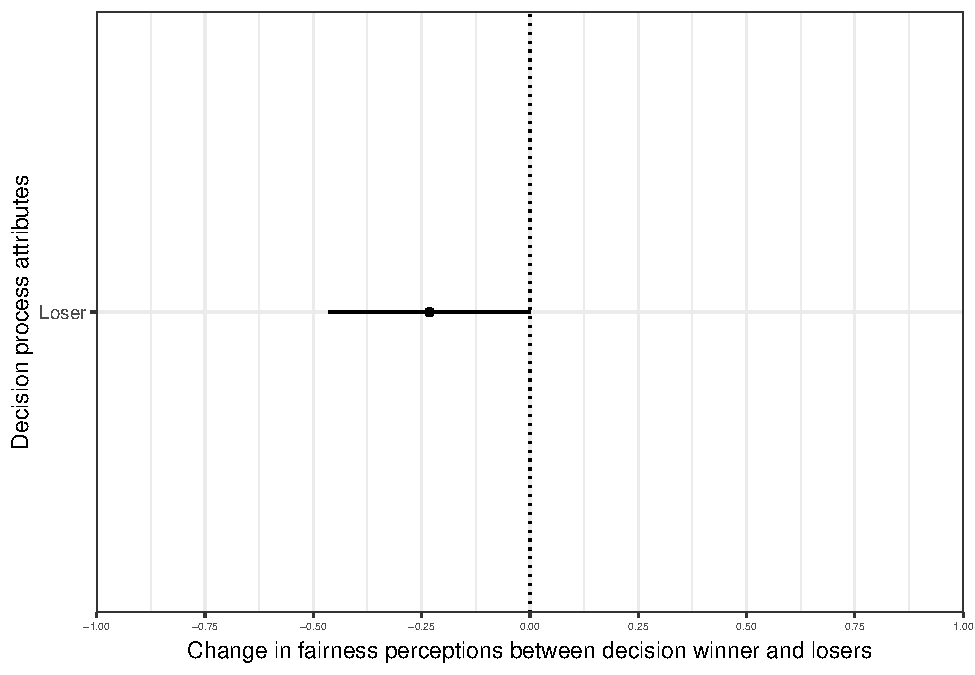
\includegraphics{Goodloser-appendix_files/figure-latex/104_post_fairness_favorability-1.pdf}

\begin{Shaded}
\begin{Highlighting}[]
\KeywordTok{ggsave}\NormalTok{(}
  \KeywordTok{here}\NormalTok{(}\StringTok{"output"}\NormalTok{, }\StringTok{"swevig"}\NormalTok{, }\StringTok{"figs"}\NormalTok{, }\StringTok{"pngs"}\NormalTok{, }\StringTok{"exp1-fairness-favorability.png"}\NormalTok{),}
  \DataTypeTok{plot =}\NormalTok{ fig,}
  \DataTypeTok{width =} \FloatTok{5.5}\NormalTok{, }\DataTypeTok{height =} \FloatTok{2.75}
\NormalTok{)}

\KeywordTok{ggsave}\NormalTok{(}
  \KeywordTok{here}\NormalTok{(}\StringTok{"output"}\NormalTok{, }\StringTok{"swevig"}\NormalTok{, }\StringTok{"figs"}\NormalTok{, }\StringTok{"pdfs"}\NormalTok{, }\StringTok{"exp1-fairness-favorability.pdf"}\NormalTok{),}
  \DataTypeTok{plot =}\NormalTok{ fig,}
  \DataTypeTok{width =} \FloatTok{5.5}\NormalTok{, }\DataTypeTok{height =} \FloatTok{2.75}
\NormalTok{)}

\CommentTok{#Table}
\NormalTok{table <-}\StringTok{ }\NormalTok{res_main }\OperatorTok\StringTok{ }
\StringTok{  }\KeywordTok{select}\NormalTok{(term, estimate, std.error, statistic, p.value) }\OperatorTok\StringTok{ }
\StringTok{  }\KeywordTok{mutate}\NormalTok{(}\DataTypeTok{term =} \KeywordTok{case_when}\NormalTok{( term }\OperatorTok{==}\StringTok{ "(Intercept)"} \OperatorTok{~}\StringTok{ "Not shown"}\NormalTok{,}
\NormalTok{                    term }\OperatorTok{==}\StringTok{ "favorabilityUnfavorable"} \OperatorTok{~}\StringTok{ "Unfavorable outcome"}\NormalTok{)}
\NormalTok{         )}

\KeywordTok{kable}\NormalTok{(table, }\DataTypeTok{booktabs =} \OtherTok{TRUE}\NormalTok{, }\DataTypeTok{caption =} \StringTok{"Difference fairness perceptions of decision between winners and losers, Study 1 -- Swedish vignette"}\NormalTok{, }\DataTypeTok{col.names =} \KeywordTok{linebreak}\NormalTok{(}\KeywordTok{c}\NormalTok{(}\StringTok{"Treatment value"}\NormalTok{, }\StringTok{"Estimate"}\NormalTok{, }\StringTok{"Std. Error"}\NormalTok{, }\StringTok{"t-statistic"}\NormalTok{, }\StringTok{"p value"}\NormalTok{))) }\OperatorTok\StringTok{ }
\StringTok{  }\KeywordTok{kable_styling}\NormalTok{(}\DataTypeTok{bootstrap_options =} \KeywordTok{c}\NormalTok{(}\StringTok{"striped"}\NormalTok{, }\StringTok{"hover"}\NormalTok{, }\StringTok{"responsive"}\NormalTok{)) }
\end{Highlighting}
\end{Shaded}

(\#tab:104\_post\_fairness\_favorability)Difference fairness perceptions
of decision between winners and losers, Study 1 -- Swedish vignette

Treatment value

Estimate

Std. Error

t-statistic

p value

Not shown

4.4564460

0.0769648

57.902377

0.0000000

Unfavorable outcome

-0.2317269

0.1164660

-1.989652

0.0468968

\subsection{Priming effects}\label{priming-effects}

\begin{Shaded}
\begin{Highlighting}[]
\NormalTok{res_main <-}\StringTok{  }\KeywordTok{lm}\NormalTok{(fairness }\OperatorTok{~}\StringTok{ }\NormalTok{treatment, }\DataTypeTok{data =}\NormalTok{ d) }
\NormalTok{res_main <-}\StringTok{ }\NormalTok{broom}\OperatorTok{::}\KeywordTok{tidy}\NormalTok{(res_main)}

\NormalTok{labels <-}\StringTok{ }\KeywordTok{data.frame}\NormalTok{(}
  \DataTypeTok{term =} \KeywordTok{c}\NormalTok{(}
    \StringTok{"treatmentLamenting politician"}\NormalTok{,}
    \StringTok{"treatmentGeneral prime"}
    
\NormalTok{  ),}
  \DataTypeTok{label =} \KeywordTok{c}\NormalTok{( }\StringTok{"Lamenting politician"}\NormalTok{,}
             \StringTok{"General prime"}\NormalTok{)}
\NormalTok{)}
\CommentTok{#Figure}
\NormalTok{fig <-}\StringTok{   }\NormalTok{res_main }\OperatorTok
\StringTok{  }\KeywordTok{filter}\NormalTok{(term }\OperatorTok{!=}\StringTok{ "(Intercept)"}\NormalTok{) }\OperatorTok\StringTok{ }
\StringTok{  }\KeywordTok{left_join}\NormalTok{(labels, }\DataTypeTok{by =} \StringTok{"term"}\NormalTok{) }\OperatorTok\StringTok{ }
\StringTok{  }
\StringTok{  }\KeywordTok{ggplot}\NormalTok{(}\KeywordTok{aes}\NormalTok{(}\DataTypeTok{x =}\NormalTok{ estimate, }\DataTypeTok{y =}\NormalTok{ label,}
             \DataTypeTok{xmin =}\NormalTok{ estimate }\OperatorTok{-}\StringTok{ }\NormalTok{(}\DecValTok{2} \OperatorTok{*}\StringTok{ }\NormalTok{std.error),}
             \DataTypeTok{xmax =}\NormalTok{ estimate }\OperatorTok{+}\StringTok{ }\NormalTok{(}\DecValTok{2} \OperatorTok{*}\StringTok{ }\NormalTok{std.error))) }\OperatorTok{+}
\StringTok{   }\KeywordTok{geom_errorbarh}\NormalTok{(}\DataTypeTok{height =} \DecValTok{0}\NormalTok{) }\OperatorTok{+}
\StringTok{  }\KeywordTok{geom_point}\NormalTok{() }\OperatorTok{+}
\StringTok{  }\KeywordTok{geom_vline}\NormalTok{(}\KeywordTok{aes}\NormalTok{(}\DataTypeTok{xintercept =} \DecValTok{0}\NormalTok{), }\DataTypeTok{linetype =} \StringTok{"dotted"}\NormalTok{) }\OperatorTok{+}
\StringTok{  }\KeywordTok{scale_x_continuous}\NormalTok{(}\DataTypeTok{limits =} \KeywordTok{c}\NormalTok{(}\OperatorTok{-}\DecValTok{1}\NormalTok{, }\DecValTok{1}\NormalTok{),}
                     \DataTypeTok{breaks =} \KeywordTok{round}\NormalTok{(}\KeywordTok{seq}\NormalTok{(}\OperatorTok{-}\DecValTok{1}\NormalTok{, }\DecValTok{1}\NormalTok{, .}\DecValTok{25}\NormalTok{), }\DecValTok{2}\NormalTok{),}
                     \DataTypeTok{expand =} \KeywordTok{c}\NormalTok{(}\DecValTok{0}\NormalTok{, }\DecValTok{0}\NormalTok{)) }\OperatorTok{+}
\StringTok{  }\KeywordTok{labs}\NormalTok{(}\DataTypeTok{x =} \StringTok{"Change in fairness perception"}\NormalTok{,}
       \DataTypeTok{y =} \StringTok{"Decision process attributes"}\NormalTok{) }\OperatorTok{+}
\StringTok{  }\KeywordTok{theme_bw}\NormalTok{() }\OperatorTok{+}
\StringTok{  }\KeywordTok{theme}\NormalTok{(}\DataTypeTok{plot.margin =} \KeywordTok{unit}\NormalTok{(}\KeywordTok{c}\NormalTok{(}\DecValTok{2}\NormalTok{, }\DecValTok{2}\NormalTok{, }\DecValTok{2}\NormalTok{, }\DecValTok{2}\NormalTok{), }\StringTok{"mm"}\NormalTok{), }\DataTypeTok{axis.text.x=}\KeywordTok{element_text}\NormalTok{(}\DataTypeTok{size=}\KeywordTok{rel}\NormalTok{(}\FloatTok{0.6}\NormalTok{))) }\OperatorTok{+}
\StringTok{  }\KeywordTok{theme}\NormalTok{(}\DataTypeTok{panel.spacing =} \KeywordTok{unit}\NormalTok{(}\FloatTok{0.5}\NormalTok{, }\StringTok{"lines"}\NormalTok{))}
\NormalTok{fig}
\end{Highlighting}
\end{Shaded}

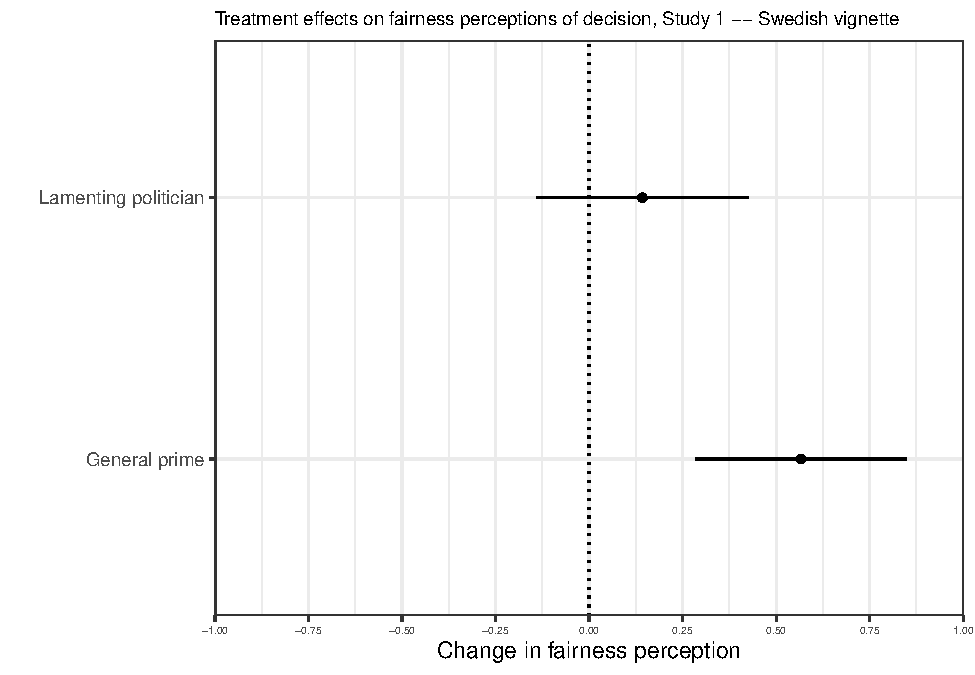
\includegraphics{Goodloser-appendix_files/figure-latex/104_post_fairness-1.pdf}

\begin{Shaded}
\begin{Highlighting}[]
\KeywordTok{ggsave}\NormalTok{(}
  \KeywordTok{here}\NormalTok{(}\StringTok{"output"}\NormalTok{, }\StringTok{"swevig"}\NormalTok{, }\StringTok{"figs"}\NormalTok{, }\StringTok{"pngs"}\NormalTok{, }\StringTok{"exp1-fairness-mainfig.png"}\NormalTok{),}
  \DataTypeTok{plot =}\NormalTok{ fig,}
  \DataTypeTok{width =} \FloatTok{5.5}\NormalTok{, }\DataTypeTok{height =} \FloatTok{2.75}
\NormalTok{)}

\KeywordTok{ggsave}\NormalTok{(}
  \KeywordTok{here}\NormalTok{(}\StringTok{"output"}\NormalTok{, }\StringTok{"swevig"}\NormalTok{, }\StringTok{"figs"}\NormalTok{, }\StringTok{"pdfs"}\NormalTok{, }\StringTok{"exp1-fairness-mainfig.pdf"}\NormalTok{),}
  \DataTypeTok{plot =}\NormalTok{ fig,}
  \DataTypeTok{width =} \FloatTok{5.5}\NormalTok{, }\DataTypeTok{height =} \FloatTok{2.75}
\NormalTok{)}


\CommentTok{#Table}
\NormalTok{table <-}\StringTok{ }\NormalTok{res_main }\OperatorTok\StringTok{ }
\StringTok{  }\KeywordTok{select}\NormalTok{(term, estimate, std.error, statistic, p.value) }\OperatorTok\StringTok{ }
\StringTok{  }\KeywordTok{mutate}\NormalTok{(}\DataTypeTok{term =} \KeywordTok{case_when}\NormalTok{( term }\OperatorTok{==}\StringTok{ "(Intercept)"} \OperatorTok{~}\StringTok{ "Not shown"}\NormalTok{,}
\NormalTok{                    term }\OperatorTok{==}\StringTok{ "treatmentLamenting politician"} \OperatorTok{~}\StringTok{ "Lamenting politician"}\NormalTok{,}
\NormalTok{                   term }\OperatorTok{==}\StringTok{ "treatmentGeneral prime"} \OperatorTok{~}\StringTok{ "General prime"}\NormalTok{)}
\NormalTok{         )}

\KeywordTok{kable}\NormalTok{(table, }\DataTypeTok{booktabs =} \OtherTok{TRUE}\NormalTok{, }\DataTypeTok{caption =} \StringTok{"Treatment effects on fairness perceptions of decision, Study 1 -- Swedish vignette"}\NormalTok{, }\DataTypeTok{col.names =} \KeywordTok{linebreak}\NormalTok{(}\KeywordTok{c}\NormalTok{(}\StringTok{"Treatment value"}\NormalTok{, }\StringTok{"Estimate"}\NormalTok{, }\StringTok{"Std. Error"}\NormalTok{, }\StringTok{"t-statistic"}\NormalTok{, }\StringTok{"p value"}\NormalTok{))) }\OperatorTok\StringTok{ }
\StringTok{  }\KeywordTok{kable_styling}\NormalTok{(}\DataTypeTok{bootstrap_options =} \KeywordTok{c}\NormalTok{(}\StringTok{"striped"}\NormalTok{, }\StringTok{"hover"}\NormalTok{, }\StringTok{"responsive"}\NormalTok{)) }
\end{Highlighting}
\end{Shaded}

(\#tab:104\_post\_fairness)Treatment effects on fairness perceptions of
decision, Study 1 -- Swedish vignette

Treatment value

Estimate

Std. Error

t-statistic

p value

Not shown

4.1138462

0.1016588

40.467206

0.0000000

Lamenting politician

0.1426380

0.1414701

1.008255

0.3135720

General prime

0.5662691

0.1414701

4.002747

0.0000672

\section{Justice}\label{justice}

\begin{Shaded}
\begin{Highlighting}[]
\NormalTok{res_main <-}\StringTok{  }\KeywordTok{lm}\NormalTok{(justice }\OperatorTok{~}\StringTok{ }\NormalTok{treatment, }\DataTypeTok{data =}\NormalTok{ d) }
\NormalTok{res_main <-}\StringTok{ }\NormalTok{broom}\OperatorTok{::}\KeywordTok{tidy}\NormalTok{(res_main)}

\NormalTok{labels <-}\StringTok{ }\KeywordTok{data.frame}\NormalTok{(}
  \DataTypeTok{term =} \KeywordTok{c}\NormalTok{(}
    \StringTok{"treatmentLamenting politician"}\NormalTok{,}
    \StringTok{"treatmentGeneral prime"}
    
\NormalTok{  ),}
  \DataTypeTok{label =} \KeywordTok{c}\NormalTok{( }\StringTok{"Lamenting politician"}\NormalTok{,}
             \StringTok{"General prime"}\NormalTok{)}
\NormalTok{)}
\CommentTok{#Figure}
\NormalTok{fig <-}\StringTok{   }\NormalTok{res_main }\OperatorTok
\StringTok{  }\KeywordTok{filter}\NormalTok{(term }\OperatorTok{!=}\StringTok{ "(Intercept)"}\NormalTok{) }\OperatorTok\StringTok{ }
\StringTok{  }\KeywordTok{left_join}\NormalTok{(labels, }\DataTypeTok{by =} \StringTok{"term"}\NormalTok{) }\OperatorTok\StringTok{ }
\StringTok{  }
\StringTok{  }\KeywordTok{ggplot}\NormalTok{(}\KeywordTok{aes}\NormalTok{(}\DataTypeTok{x =}\NormalTok{ estimate, }\DataTypeTok{y =}\NormalTok{ label,}
             \DataTypeTok{xmin =}\NormalTok{ estimate }\OperatorTok{-}\StringTok{ }\NormalTok{(}\DecValTok{2} \OperatorTok{*}\StringTok{ }\NormalTok{std.error),}
             \DataTypeTok{xmax =}\NormalTok{ estimate }\OperatorTok{+}\StringTok{ }\NormalTok{(}\DecValTok{2} \OperatorTok{*}\StringTok{ }\NormalTok{std.error))) }\OperatorTok{+}
\StringTok{   }\KeywordTok{geom_errorbarh}\NormalTok{(}\DataTypeTok{height =} \DecValTok{0}\NormalTok{) }\OperatorTok{+}
\StringTok{  }\KeywordTok{geom_point}\NormalTok{() }\OperatorTok{+}
\StringTok{  }\KeywordTok{geom_vline}\NormalTok{(}\KeywordTok{aes}\NormalTok{(}\DataTypeTok{xintercept =} \DecValTok{0}\NormalTok{), }\DataTypeTok{linetype =} \StringTok{"dotted"}\NormalTok{) }\OperatorTok{+}
\StringTok{  }\KeywordTok{scale_x_continuous}\NormalTok{(}\DataTypeTok{limits =} \KeywordTok{c}\NormalTok{(}\OperatorTok{-}\DecValTok{1}\NormalTok{, }\DecValTok{1}\NormalTok{),}
                     \DataTypeTok{breaks =} \KeywordTok{round}\NormalTok{(}\KeywordTok{seq}\NormalTok{(}\OperatorTok{-}\DecValTok{1}\NormalTok{, }\DecValTok{1}\NormalTok{, .}\DecValTok{25}\NormalTok{), }\DecValTok{2}\NormalTok{),}
                     \DataTypeTok{expand =} \KeywordTok{c}\NormalTok{(}\DecValTok{0}\NormalTok{, }\DecValTok{0}\NormalTok{)) }\OperatorTok{+}
\StringTok{  }\KeywordTok{labs}\NormalTok{(}\DataTypeTok{x =} \StringTok{"Change in justice perception"}\NormalTok{,}
       \DataTypeTok{y =} \StringTok{"Decision process attributes"}\NormalTok{) }\OperatorTok{+}
\StringTok{  }\KeywordTok{theme_bw}\NormalTok{() }\OperatorTok{+}
\StringTok{  }\KeywordTok{theme}\NormalTok{(}\DataTypeTok{plot.margin =} \KeywordTok{unit}\NormalTok{(}\KeywordTok{c}\NormalTok{(}\DecValTok{2}\NormalTok{, }\DecValTok{2}\NormalTok{, }\DecValTok{2}\NormalTok{, }\DecValTok{2}\NormalTok{), }\StringTok{"mm"}\NormalTok{), }\DataTypeTok{axis.text.x=}\KeywordTok{element_text}\NormalTok{(}\DataTypeTok{size=}\KeywordTok{rel}\NormalTok{(}\FloatTok{0.6}\NormalTok{))) }\OperatorTok{+}
\StringTok{  }\KeywordTok{theme}\NormalTok{(}\DataTypeTok{panel.spacing =} \KeywordTok{unit}\NormalTok{(}\FloatTok{0.5}\NormalTok{, }\StringTok{"lines"}\NormalTok{))}
\NormalTok{fig}
\end{Highlighting}
\end{Shaded}

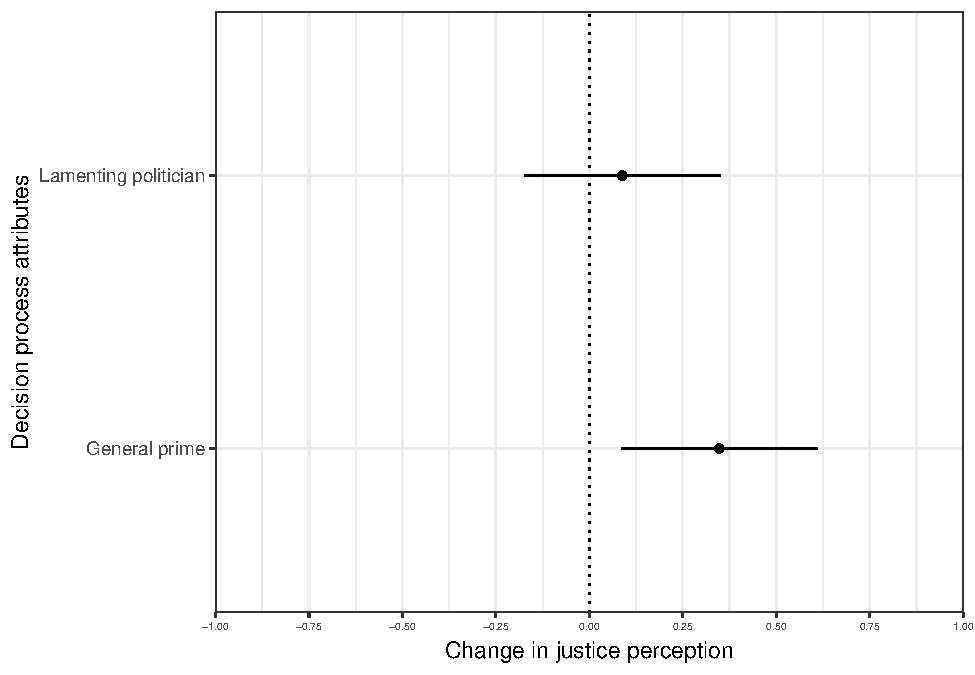
\includegraphics{Goodloser-appendix_files/figure-latex/104_post_justice-1.pdf}

\begin{Shaded}
\begin{Highlighting}[]
\KeywordTok{ggsave}\NormalTok{(}
  \KeywordTok{here}\NormalTok{(}\StringTok{"output"}\NormalTok{, }\StringTok{"swevig"}\NormalTok{, }\StringTok{"figs"}\NormalTok{, }\StringTok{"pngs"}\NormalTok{, }\StringTok{"exp1-justice-mainfig.png"}\NormalTok{),}
  \DataTypeTok{plot =}\NormalTok{ fig,}
  \DataTypeTok{width =} \FloatTok{5.5}\NormalTok{, }\DataTypeTok{height =} \FloatTok{2.75}
\NormalTok{)}

\KeywordTok{ggsave}\NormalTok{(}
  \KeywordTok{here}\NormalTok{(}\StringTok{"output"}\NormalTok{, }\StringTok{"swevig"}\NormalTok{, }\StringTok{"figs"}\NormalTok{, }\StringTok{"pdfs"}\NormalTok{, }\StringTok{"exp1-justice-mainfig.pdf"}\NormalTok{),}
  \DataTypeTok{plot =}\NormalTok{ fig,}
  \DataTypeTok{width =} \FloatTok{5.5}\NormalTok{, }\DataTypeTok{height =} \FloatTok{2.75}
\NormalTok{)}


\CommentTok{#Table}
\NormalTok{table <-}\StringTok{ }\NormalTok{res_main }\OperatorTok\StringTok{ }
\StringTok{  }\KeywordTok{select}\NormalTok{(term, estimate, std.error, statistic, p.value) }\OperatorTok\StringTok{ }
\StringTok{  }\KeywordTok{mutate}\NormalTok{(}\DataTypeTok{term =} \KeywordTok{case_when}\NormalTok{( term }\OperatorTok{==}\StringTok{ "(Intercept)"} \OperatorTok{~}\StringTok{ "Not shown"}\NormalTok{,}
\NormalTok{                    term }\OperatorTok{==}\StringTok{ "treatmentLamenting politician"} \OperatorTok{~}\StringTok{ "Lamenting politician"}\NormalTok{,}
\NormalTok{                   term }\OperatorTok{==}\StringTok{ "treatmentGeneral prime"} \OperatorTok{~}\StringTok{ "General prime"}\NormalTok{)}
\NormalTok{         )}

\KeywordTok{kable}\NormalTok{(table, }\DataTypeTok{booktabs =} \OtherTok{TRUE}\NormalTok{, }\DataTypeTok{caption =} \StringTok{"Treatment effects on justice perceptions of decision, Study 1 -- Swedish vignette"}\NormalTok{, }\DataTypeTok{col.names =} \KeywordTok{linebreak}\NormalTok{(}\KeywordTok{c}\NormalTok{(}\StringTok{"Treatment value"}\NormalTok{, }\StringTok{"Estimate"}\NormalTok{, }\StringTok{"Std. Error"}\NormalTok{, }\StringTok{"t-statistic"}\NormalTok{, }\StringTok{"p value"}\NormalTok{))) }\OperatorTok\StringTok{ }
\StringTok{  }\KeywordTok{kable_styling}\NormalTok{(}\DataTypeTok{bootstrap_options =} \KeywordTok{c}\NormalTok{(}\StringTok{"striped"}\NormalTok{, }\StringTok{"hover"}\NormalTok{, }\StringTok{"responsive"}\NormalTok{)) }
\end{Highlighting}
\end{Shaded}

(\#tab:104\_post\_justice)Treatment effects on justice perceptions of
decision, Study 1 -- Swedish vignette

Treatment value

Estimate

Std. Error

t-statistic

p value

Not shown

4.0615385

0.0943412

43.0515828

0.0000000

Lamenting politician

0.0883174

0.1312869

0.6727058

0.5012875

General prime

0.3476834

0.1312869

2.6482724

0.0082158

\section{Decision evaluation}\label{decision-evaluation}

\begin{Shaded}
\begin{Highlighting}[]
\NormalTok{res_main <-}\StringTok{  }\KeywordTok{lm}\NormalTok{(eval }\OperatorTok{~}\StringTok{ }\NormalTok{treatment, }\DataTypeTok{data =}\NormalTok{ d) }
\NormalTok{res_main <-}\StringTok{ }\NormalTok{broom}\OperatorTok{::}\KeywordTok{tidy}\NormalTok{(res_main)}

\NormalTok{labels <-}\StringTok{ }\KeywordTok{data.frame}\NormalTok{(}
  \DataTypeTok{term =} \KeywordTok{c}\NormalTok{(}
    \StringTok{"treatmentLamenting politician"}\NormalTok{,}
    \StringTok{"treatmentGeneral prime"}
    
\NormalTok{  ),}
  \DataTypeTok{label =} \KeywordTok{c}\NormalTok{( }\StringTok{"Lamenting politician"}\NormalTok{,}
             \StringTok{"General prime"}\NormalTok{)}
\NormalTok{)}
\CommentTok{#Figure}
\NormalTok{fig <-}\StringTok{   }\NormalTok{res_main }\OperatorTok
\StringTok{  }\KeywordTok{filter}\NormalTok{(term }\OperatorTok{!=}\StringTok{ "(Intercept)"}\NormalTok{) }\OperatorTok\StringTok{ }
\StringTok{  }\KeywordTok{left_join}\NormalTok{(labels, }\DataTypeTok{by =} \StringTok{"term"}\NormalTok{) }\OperatorTok\StringTok{ }
\StringTok{  }
\StringTok{  }\KeywordTok{ggplot}\NormalTok{(}\KeywordTok{aes}\NormalTok{(}\DataTypeTok{x =}\NormalTok{ estimate, }\DataTypeTok{y =}\NormalTok{ label,}
             \DataTypeTok{xmin =}\NormalTok{ estimate }\OperatorTok{-}\StringTok{ }\NormalTok{(}\DecValTok{2} \OperatorTok{*}\StringTok{ }\NormalTok{std.error),}
             \DataTypeTok{xmax =}\NormalTok{ estimate }\OperatorTok{+}\StringTok{ }\NormalTok{(}\DecValTok{2} \OperatorTok{*}\StringTok{ }\NormalTok{std.error))) }\OperatorTok{+}
\StringTok{   }\KeywordTok{geom_errorbarh}\NormalTok{(}\DataTypeTok{height =} \DecValTok{0}\NormalTok{) }\OperatorTok{+}
\StringTok{  }\KeywordTok{geom_point}\NormalTok{() }\OperatorTok{+}
\StringTok{  }\KeywordTok{geom_vline}\NormalTok{(}\KeywordTok{aes}\NormalTok{(}\DataTypeTok{xintercept =} \DecValTok{0}\NormalTok{), }\DataTypeTok{linetype =} \StringTok{"dotted"}\NormalTok{) }\OperatorTok{+}
\StringTok{  }\KeywordTok{scale_x_continuous}\NormalTok{(}\DataTypeTok{limits =} \KeywordTok{c}\NormalTok{(}\OperatorTok{-}\DecValTok{1}\NormalTok{, }\DecValTok{1}\NormalTok{),}
                     \DataTypeTok{breaks =} \KeywordTok{round}\NormalTok{(}\KeywordTok{seq}\NormalTok{(}\OperatorTok{-}\DecValTok{1}\NormalTok{, }\DecValTok{1}\NormalTok{, .}\DecValTok{25}\NormalTok{), }\DecValTok{2}\NormalTok{),}
                     \DataTypeTok{expand =} \KeywordTok{c}\NormalTok{(}\DecValTok{0}\NormalTok{, }\DecValTok{0}\NormalTok{)) }\OperatorTok{+}
\StringTok{  }\KeywordTok{labs}\NormalTok{(}\DataTypeTok{x =} \StringTok{"Change in decision evaluation"}\NormalTok{,}
       \DataTypeTok{y =} \StringTok{"Decision process attributes"}\NormalTok{) }\OperatorTok{+}
\StringTok{  }\KeywordTok{theme_bw}\NormalTok{() }\OperatorTok{+}
\StringTok{  }\KeywordTok{theme}\NormalTok{(}\DataTypeTok{plot.margin =} \KeywordTok{unit}\NormalTok{(}\KeywordTok{c}\NormalTok{(}\DecValTok{2}\NormalTok{, }\DecValTok{2}\NormalTok{, }\DecValTok{2}\NormalTok{, }\DecValTok{2}\NormalTok{), }\StringTok{"mm"}\NormalTok{), }\DataTypeTok{axis.text.x=}\KeywordTok{element_text}\NormalTok{(}\DataTypeTok{size=}\KeywordTok{rel}\NormalTok{(}\FloatTok{0.7}\NormalTok{))) }\OperatorTok{+}
\StringTok{  }\KeywordTok{theme}\NormalTok{(}\DataTypeTok{panel.spacing =} \KeywordTok{unit}\NormalTok{(}\FloatTok{0.5}\NormalTok{, }\StringTok{"lines"}\NormalTok{))}
\NormalTok{fig}
\end{Highlighting}
\end{Shaded}

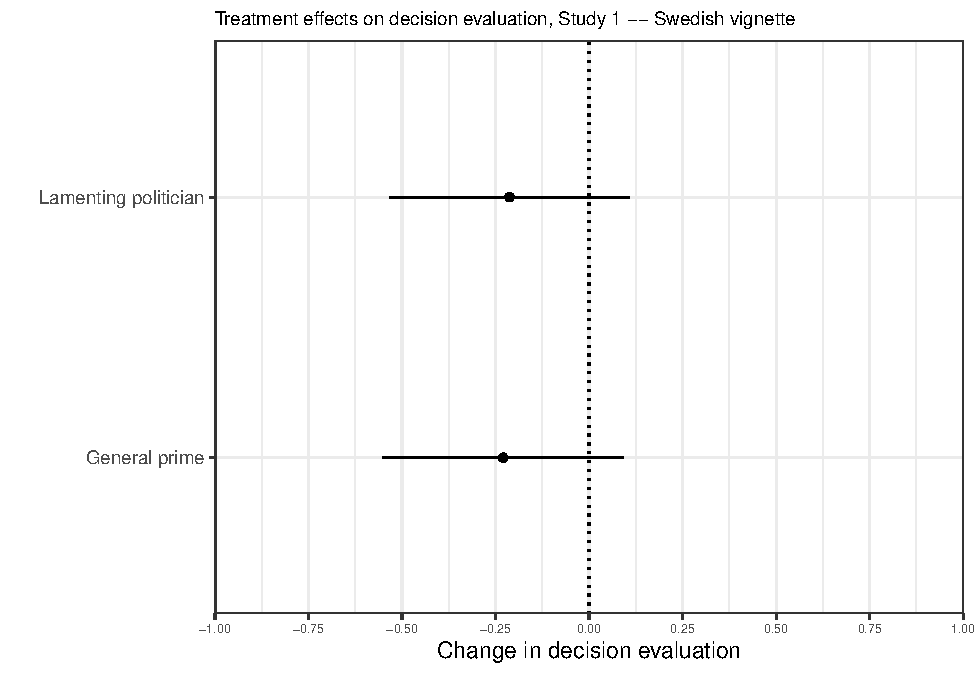
\includegraphics{Goodloser-appendix_files/figure-latex/104_post_eval-1.pdf}

\begin{Shaded}
\begin{Highlighting}[]
\KeywordTok{ggsave}\NormalTok{(}
  \KeywordTok{here}\NormalTok{(}\StringTok{"output"}\NormalTok{, }\StringTok{"swevig"}\NormalTok{, }\StringTok{"figs"}\NormalTok{, }\StringTok{"pngs"}\NormalTok{, }\StringTok{"exp1-eval-mainfig.png"}\NormalTok{),}
  \DataTypeTok{plot =}\NormalTok{ fig,}
  \DataTypeTok{width =} \FloatTok{5.5}\NormalTok{, }\DataTypeTok{height =} \FloatTok{2.75}
\NormalTok{)}

\KeywordTok{ggsave}\NormalTok{(}
  \KeywordTok{here}\NormalTok{(}\StringTok{"output"}\NormalTok{, }\StringTok{"swevig"}\NormalTok{, }\StringTok{"figs"}\NormalTok{, }\StringTok{"pdfs"}\NormalTok{, }\StringTok{"exp1-eval-mainfig.pdf"}\NormalTok{),}
  \DataTypeTok{plot =}\NormalTok{ fig,}
  \DataTypeTok{width =} \FloatTok{5.5}\NormalTok{, }\DataTypeTok{height =} \FloatTok{2.75}
\NormalTok{)}


\CommentTok{#Table}
\NormalTok{table <-}\StringTok{ }\NormalTok{res_main }\OperatorTok\StringTok{ }
\StringTok{  }\KeywordTok{select}\NormalTok{(term, estimate, std.error, statistic, p.value) }\OperatorTok\StringTok{ }
\StringTok{  }\KeywordTok{mutate}\NormalTok{(}\DataTypeTok{term =} \KeywordTok{case_when}\NormalTok{( term }\OperatorTok{==}\StringTok{ "(Intercept)"} \OperatorTok{~}\StringTok{ "Not shown"}\NormalTok{,}
\NormalTok{                    term }\OperatorTok{==}\StringTok{ "treatmentLamenting politician"} \OperatorTok{~}\StringTok{ "Lamenting politician"}\NormalTok{,}
\NormalTok{                   term }\OperatorTok{==}\StringTok{ "treatmentGeneral prime"} \OperatorTok{~}\StringTok{ "General prime"}\NormalTok{)}
\NormalTok{         )}

\KeywordTok{kable}\NormalTok{(table, }\DataTypeTok{booktabs =} \OtherTok{TRUE}\NormalTok{, }\DataTypeTok{caption =} \StringTok{"Treatment effects on decision evaluation, Study 1 -- Swedish vignette"}\NormalTok{, }\DataTypeTok{col.names =} \KeywordTok{linebreak}\NormalTok{(}\KeywordTok{c}\NormalTok{(}\StringTok{"Treatment value"}\NormalTok{, }\StringTok{"Estimate"}\NormalTok{, }\StringTok{"Std. Error"}\NormalTok{, }\StringTok{"t-statistic"}\NormalTok{, }\StringTok{"p value"}\NormalTok{))) }\OperatorTok\StringTok{ }
\StringTok{  }\KeywordTok{kable_styling}\NormalTok{(}\DataTypeTok{bootstrap_options =} \KeywordTok{c}\NormalTok{(}\StringTok{"striped"}\NormalTok{, }\StringTok{"hover"}\NormalTok{, }\StringTok{"responsive"}\NormalTok{)) }
\end{Highlighting}
\end{Shaded}

(\#tab:104\_post\_eval)Treatment effects on decision evaluation, Study 1
-- Swedish vignette

Treatment value

Estimate

Std. Error

t-statistic

p value

Not shown

4.3076923

0.1154874

37.300098

0.0000000

Lamenting politician

-0.2125914

0.1607143

-1.322791

0.1862026

General prime

-0.2298825

0.1607143

-1.430380

0.1529155

\section{Willingness to accept}\label{willingness-to-accept}

\begin{Shaded}
\begin{Highlighting}[]
\NormalTok{res_main <-}\StringTok{  }\KeywordTok{lm}\NormalTok{(accept }\OperatorTok{~}\StringTok{ }\NormalTok{treatment, }\DataTypeTok{data =}\NormalTok{ d) }
\NormalTok{res_main <-}\StringTok{ }\NormalTok{broom}\OperatorTok{::}\KeywordTok{tidy}\NormalTok{(res_main)}

\NormalTok{labels <-}\StringTok{ }\KeywordTok{data.frame}\NormalTok{(}
  \DataTypeTok{term =} \KeywordTok{c}\NormalTok{(}
    \StringTok{"treatmentLamenting politician"}\NormalTok{,}
    \StringTok{"treatmentGeneral prime"}
    
\NormalTok{  ),}
  \DataTypeTok{label =} \KeywordTok{c}\NormalTok{( }\StringTok{"Lamenting politician"}\NormalTok{,}
             \StringTok{"General prime"}\NormalTok{)}
\NormalTok{)}
\CommentTok{#Figure}
\NormalTok{fig <-}\StringTok{   }\NormalTok{res_main }\OperatorTok
\StringTok{  }\KeywordTok{filter}\NormalTok{(term }\OperatorTok{!=}\StringTok{ "(Intercept)"}\NormalTok{) }\OperatorTok\StringTok{ }
\StringTok{  }\KeywordTok{left_join}\NormalTok{(labels, }\DataTypeTok{by =} \StringTok{"term"}\NormalTok{) }\OperatorTok\StringTok{ }
\StringTok{  }
\StringTok{  }\KeywordTok{ggplot}\NormalTok{(}\KeywordTok{aes}\NormalTok{(}\DataTypeTok{x =}\NormalTok{ estimate, }\DataTypeTok{y =}\NormalTok{ label,}
             \DataTypeTok{xmin =}\NormalTok{ estimate }\OperatorTok{-}\StringTok{ }\NormalTok{(}\DecValTok{2} \OperatorTok{*}\StringTok{ }\NormalTok{std.error),}
             \DataTypeTok{xmax =}\NormalTok{ estimate }\OperatorTok{+}\StringTok{ }\NormalTok{(}\DecValTok{2} \OperatorTok{*}\StringTok{ }\NormalTok{std.error))) }\OperatorTok{+}
\StringTok{   }\KeywordTok{geom_errorbarh}\NormalTok{(}\DataTypeTok{height =} \DecValTok{0}\NormalTok{) }\OperatorTok{+}
\StringTok{  }\KeywordTok{geom_point}\NormalTok{() }\OperatorTok{+}
\StringTok{  }\KeywordTok{geom_vline}\NormalTok{(}\KeywordTok{aes}\NormalTok{(}\DataTypeTok{xintercept =} \DecValTok{0}\NormalTok{), }\DataTypeTok{linetype =} \StringTok{"dotted"}\NormalTok{) }\OperatorTok{+}
\StringTok{  }\KeywordTok{scale_x_continuous}\NormalTok{(}\DataTypeTok{limits =} \KeywordTok{c}\NormalTok{(}\OperatorTok{-}\DecValTok{1}\NormalTok{, }\DecValTok{1}\NormalTok{),}
                     \DataTypeTok{breaks =} \KeywordTok{round}\NormalTok{(}\KeywordTok{seq}\NormalTok{(}\OperatorTok{-}\DecValTok{1}\NormalTok{, }\DecValTok{1}\NormalTok{, .}\DecValTok{25}\NormalTok{), }\DecValTok{2}\NormalTok{),}
                     \DataTypeTok{expand =} \KeywordTok{c}\NormalTok{(}\DecValTok{0}\NormalTok{, }\DecValTok{0}\NormalTok{)) }\OperatorTok{+}
\StringTok{  }\KeywordTok{labs}\NormalTok{(}\DataTypeTok{x =} \StringTok{"Change in willingness to accept outcome"}\NormalTok{,}
       \DataTypeTok{y =} \StringTok{"Decision process attributes"}\NormalTok{) }\OperatorTok{+}
\StringTok{  }\KeywordTok{theme_bw}\NormalTok{() }\OperatorTok{+}
\StringTok{  }\KeywordTok{theme}\NormalTok{(}\DataTypeTok{plot.margin =} \KeywordTok{unit}\NormalTok{(}\KeywordTok{c}\NormalTok{(}\DecValTok{2}\NormalTok{, }\DecValTok{2}\NormalTok{, }\DecValTok{2}\NormalTok{, }\DecValTok{2}\NormalTok{), }\StringTok{"mm"}\NormalTok{), }\DataTypeTok{axis.text.x=}\KeywordTok{element_text}\NormalTok{(}\DataTypeTok{size=}\KeywordTok{rel}\NormalTok{(}\FloatTok{0.6}\NormalTok{))) }\OperatorTok{+}
\StringTok{  }\KeywordTok{theme}\NormalTok{(}\DataTypeTok{panel.spacing =} \KeywordTok{unit}\NormalTok{(}\FloatTok{0.5}\NormalTok{, }\StringTok{"lines"}\NormalTok{))}
\NormalTok{fig}
\end{Highlighting}
\end{Shaded}

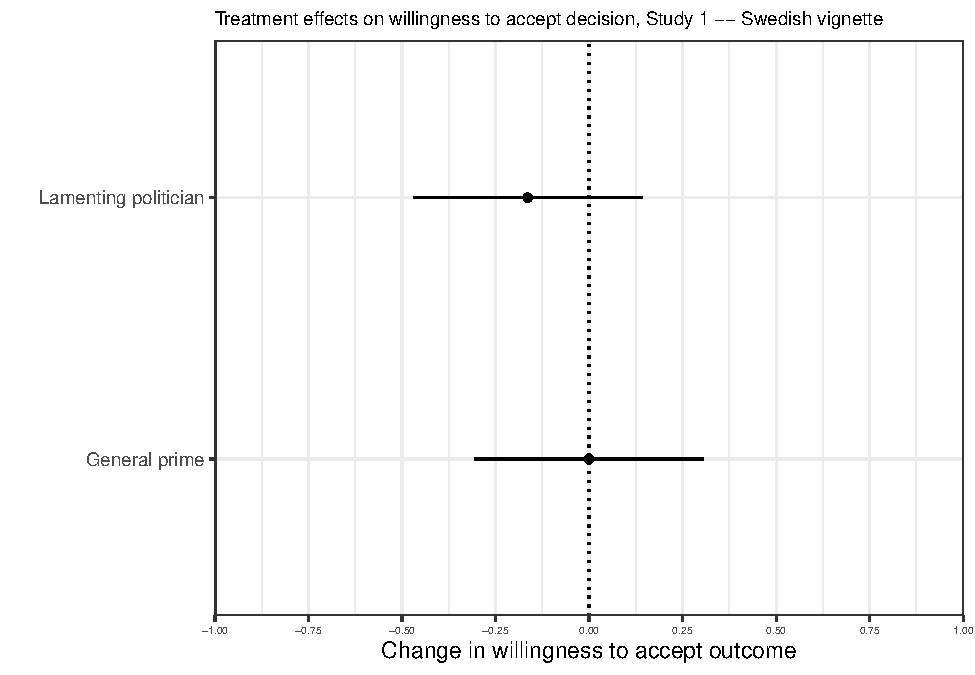
\includegraphics{Goodloser-appendix_files/figure-latex/104_post_accept-1.pdf}

\begin{Shaded}
\begin{Highlighting}[]
\KeywordTok{ggsave}\NormalTok{(}
  \KeywordTok{here}\NormalTok{(}\StringTok{"output"}\NormalTok{, }\StringTok{"swevig"}\NormalTok{, }\StringTok{"figs"}\NormalTok{, }\StringTok{"pngs"}\NormalTok{, }\StringTok{"exp1-accept-mainfig.png"}\NormalTok{),}
  \DataTypeTok{plot =}\NormalTok{ fig,}
  \DataTypeTok{width =} \FloatTok{5.5}\NormalTok{, }\DataTypeTok{height =} \FloatTok{2.75}
\NormalTok{)}

\KeywordTok{ggsave}\NormalTok{(}
  \KeywordTok{here}\NormalTok{(}\StringTok{"output"}\NormalTok{, }\StringTok{"swevig"}\NormalTok{, }\StringTok{"figs"}\NormalTok{, }\StringTok{"pdfs"}\NormalTok{, }\StringTok{"exp1-accept-mainfig.pdf"}\NormalTok{),}
  \DataTypeTok{plot =}\NormalTok{ fig,}
  \DataTypeTok{width =} \FloatTok{5.5}\NormalTok{, }\DataTypeTok{height =} \FloatTok{2.75}
\NormalTok{)}


\CommentTok{#Table}
\NormalTok{table <-}\StringTok{ }\NormalTok{res_main }\OperatorTok\StringTok{ }
\StringTok{  }\KeywordTok{select}\NormalTok{(term, estimate, std.error, statistic, p.value) }\OperatorTok\StringTok{ }
\StringTok{  }\KeywordTok{mutate}\NormalTok{(}\DataTypeTok{term =} \KeywordTok{case_when}\NormalTok{( term }\OperatorTok{==}\StringTok{ "(Intercept)"} \OperatorTok{~}\StringTok{ "Not shown"}\NormalTok{,}
\NormalTok{                    term }\OperatorTok{==}\StringTok{ "treatmentLamenting politician"} \OperatorTok{~}\StringTok{ "Lamenting politician"}\NormalTok{,}
\NormalTok{                   term }\OperatorTok{==}\StringTok{ "treatmentGeneral prime"} \OperatorTok{~}\StringTok{ "General prime"}\NormalTok{)}
\NormalTok{         )}

\KeywordTok{kable}\NormalTok{(table, }\DataTypeTok{booktabs =} \OtherTok{TRUE}\NormalTok{, }\DataTypeTok{caption =} \StringTok{"Treatment effects on willingness to accept decision, Study 1 -- Swedish vignette"}\NormalTok{, }\DataTypeTok{col.names =} \KeywordTok{linebreak}\NormalTok{(}\KeywordTok{c}\NormalTok{(}\StringTok{"Treatment value"}\NormalTok{, }\StringTok{"Estimate"}\NormalTok{, }\StringTok{"Std. Error"}\NormalTok{, }\StringTok{"t-statistic"}\NormalTok{, }\StringTok{"p value"}\NormalTok{))) }\OperatorTok\StringTok{ }
\StringTok{  }\KeywordTok{kable_styling}\NormalTok{(}\DataTypeTok{bootstrap_options =} \KeywordTok{c}\NormalTok{(}\StringTok{"striped"}\NormalTok{, }\StringTok{"hover"}\NormalTok{, }\StringTok{"responsive"}\NormalTok{)) }
\end{Highlighting}
\end{Shaded}

(\#tab:104\_post\_accept)Treatment effects on willingness to accept
decision, Study 1 -- Swedish vignette

Treatment value

Estimate

Std. Error

t-statistic

p value

Not shown

5.1784615

0.1101387

47.0176540

0.0000000

Lamenting politician

-0.1640523

0.1532709

-1.0703422

0.2847195

General prime

0.0002128

0.1532709

0.0013885

0.9988924

\section{Compliance}\label{compliance}

\begin{Shaded}
\begin{Highlighting}[]
\NormalTok{res_main <-}\StringTok{  }\KeywordTok{lm}\NormalTok{(comply }\OperatorTok{~}\StringTok{ }\NormalTok{treatment, }\DataTypeTok{data =}\NormalTok{ d) }
\NormalTok{res_main <-}\StringTok{ }\NormalTok{broom}\OperatorTok{::}\KeywordTok{tidy}\NormalTok{(res_main)}

\NormalTok{labels <-}\StringTok{ }\KeywordTok{data.frame}\NormalTok{(}
  \DataTypeTok{term =} \KeywordTok{c}\NormalTok{(}
    \StringTok{"treatmentLamenting politician"}\NormalTok{,}
    \StringTok{"treatmentGeneral prime"}
    
\NormalTok{  ),}
  \DataTypeTok{label =} \KeywordTok{c}\NormalTok{( }\StringTok{"Lamenting politician"}\NormalTok{,}
             \StringTok{"General prime"}\NormalTok{)}
\NormalTok{)}
\CommentTok{#Figure}
\NormalTok{fig <-}\StringTok{   }\NormalTok{res_main }\OperatorTok
\StringTok{  }\KeywordTok{filter}\NormalTok{(term }\OperatorTok{!=}\StringTok{ "(Intercept)"}\NormalTok{) }\OperatorTok\StringTok{ }
\StringTok{  }\KeywordTok{left_join}\NormalTok{(labels, }\DataTypeTok{by =} \StringTok{"term"}\NormalTok{) }\OperatorTok\StringTok{ }
\StringTok{  }
\StringTok{  }\KeywordTok{ggplot}\NormalTok{(}\KeywordTok{aes}\NormalTok{(}\DataTypeTok{x =}\NormalTok{ estimate, }\DataTypeTok{y =}\NormalTok{ label,}
             \DataTypeTok{xmin =}\NormalTok{ estimate }\OperatorTok{-}\StringTok{ }\NormalTok{(}\DecValTok{2} \OperatorTok{*}\StringTok{ }\NormalTok{std.error),}
             \DataTypeTok{xmax =}\NormalTok{ estimate }\OperatorTok{+}\StringTok{ }\NormalTok{(}\DecValTok{2} \OperatorTok{*}\StringTok{ }\NormalTok{std.error))) }\OperatorTok{+}
\StringTok{   }\KeywordTok{geom_errorbarh}\NormalTok{(}\DataTypeTok{height =} \DecValTok{0}\NormalTok{) }\OperatorTok{+}
\StringTok{  }\KeywordTok{geom_point}\NormalTok{() }\OperatorTok{+}
\StringTok{  }\KeywordTok{geom_vline}\NormalTok{(}\KeywordTok{aes}\NormalTok{(}\DataTypeTok{xintercept =} \DecValTok{0}\NormalTok{), }\DataTypeTok{linetype =} \StringTok{"dotted"}\NormalTok{) }\OperatorTok{+}
\StringTok{  }\KeywordTok{scale_x_continuous}\NormalTok{(}\DataTypeTok{limits =} \KeywordTok{c}\NormalTok{(}\OperatorTok{-}\DecValTok{1}\NormalTok{, }\DecValTok{1}\NormalTok{),}
                     \DataTypeTok{breaks =} \KeywordTok{round}\NormalTok{(}\KeywordTok{seq}\NormalTok{(}\OperatorTok{-}\DecValTok{1}\NormalTok{, }\DecValTok{1}\NormalTok{, .}\DecValTok{25}\NormalTok{), }\DecValTok{2}\NormalTok{),}
                     \DataTypeTok{expand =} \KeywordTok{c}\NormalTok{(}\DecValTok{0}\NormalTok{, }\DecValTok{0}\NormalTok{)) }\OperatorTok{+}
\StringTok{  }\KeywordTok{labs}\NormalTok{(}\DataTypeTok{x =} \StringTok{"Change in decision compliance"}\NormalTok{,}
       \DataTypeTok{y =} \StringTok{"Decision process attributes"}\NormalTok{) }\OperatorTok{+}
\StringTok{  }\KeywordTok{theme_bw}\NormalTok{() }\OperatorTok{+}
\StringTok{  }\KeywordTok{theme}\NormalTok{(}\DataTypeTok{plot.margin =} \KeywordTok{unit}\NormalTok{(}\KeywordTok{c}\NormalTok{(}\DecValTok{2}\NormalTok{, }\DecValTok{2}\NormalTok{, }\DecValTok{2}\NormalTok{, }\DecValTok{2}\NormalTok{), }\StringTok{"mm"}\NormalTok{), }\DataTypeTok{axis.text.x=}\KeywordTok{element_text}\NormalTok{(}\DataTypeTok{size=}\KeywordTok{rel}\NormalTok{(}\FloatTok{0.6}\NormalTok{))) }\OperatorTok{+}
\StringTok{  }\KeywordTok{theme}\NormalTok{(}\DataTypeTok{panel.spacing =} \KeywordTok{unit}\NormalTok{(}\FloatTok{0.5}\NormalTok{, }\StringTok{"lines"}\NormalTok{))}
\NormalTok{fig}
\end{Highlighting}
\end{Shaded}

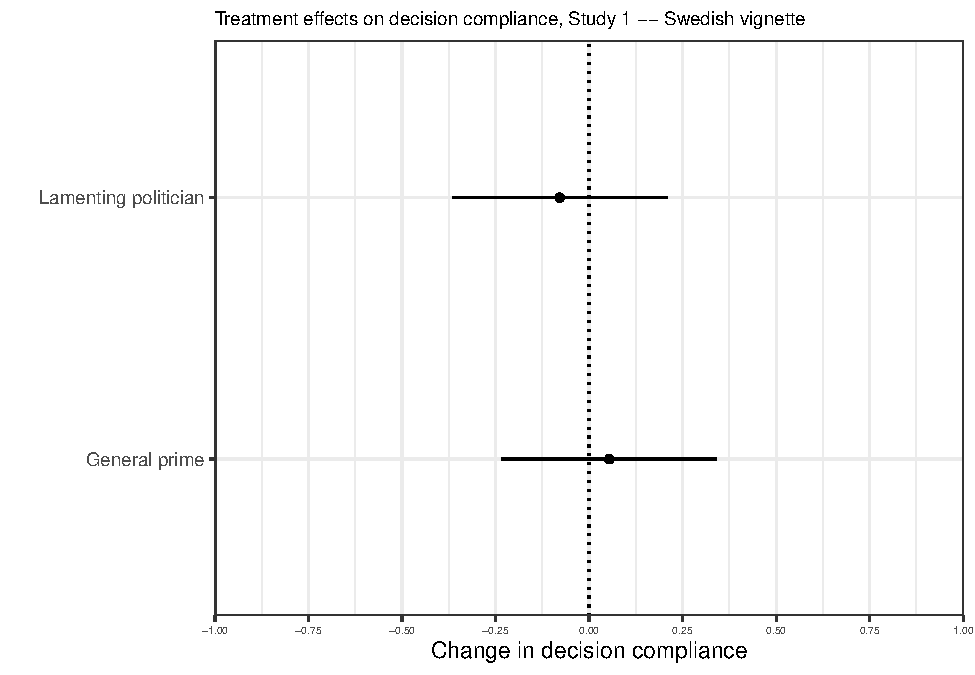
\includegraphics{Goodloser-appendix_files/figure-latex/104_post_comply-1.pdf}

\begin{Shaded}
\begin{Highlighting}[]
\KeywordTok{ggsave}\NormalTok{(}
  \KeywordTok{here}\NormalTok{(}\StringTok{"output"}\NormalTok{, }\StringTok{"swevig"}\NormalTok{, }\StringTok{"figs"}\NormalTok{, }\StringTok{"pngs"}\NormalTok{, }\StringTok{"exp1-comply-mainfig.png"}\NormalTok{),}
  \DataTypeTok{plot =}\NormalTok{ fig,}
  \DataTypeTok{width =} \FloatTok{5.5}\NormalTok{, }\DataTypeTok{height =} \FloatTok{2.75}
\NormalTok{)}

\KeywordTok{ggsave}\NormalTok{(}
  \KeywordTok{here}\NormalTok{(}\StringTok{"output"}\NormalTok{, }\StringTok{"swevig"}\NormalTok{, }\StringTok{"figs"}\NormalTok{, }\StringTok{"pdfs"}\NormalTok{, }\StringTok{"exp1-comply-mainfig.pdf"}\NormalTok{),}
  \DataTypeTok{plot =}\NormalTok{ fig,}
  \DataTypeTok{width =} \FloatTok{5.5}\NormalTok{, }\DataTypeTok{height =} \FloatTok{2.75}
\NormalTok{)}


\CommentTok{#Table}
\NormalTok{table <-}\StringTok{ }\NormalTok{res_main }\OperatorTok\StringTok{ }
\StringTok{  }\KeywordTok{select}\NormalTok{(term, estimate, std.error, statistic, p.value) }\OperatorTok\StringTok{ }
\StringTok{  }\KeywordTok{mutate}\NormalTok{(}\DataTypeTok{term =} \KeywordTok{case_when}\NormalTok{( term }\OperatorTok{==}\StringTok{ "(Intercept)"} \OperatorTok{~}\StringTok{ "Not shown"}\NormalTok{,}
\NormalTok{                    term }\OperatorTok{==}\StringTok{ "treatmentLamenting politician"} \OperatorTok{~}\StringTok{ "Lamenting politician"}\NormalTok{,}
\NormalTok{                   term }\OperatorTok{==}\StringTok{ "treatmentGeneral prime"} \OperatorTok{~}\StringTok{ "General prime"}\NormalTok{)}
\NormalTok{         )}

\KeywordTok{kable}\NormalTok{(table, }\DataTypeTok{booktabs =} \OtherTok{TRUE}\NormalTok{, }\DataTypeTok{caption =} \StringTok{"Treatment effects on decision compliance, Study 1 -- Swedish vignette"}\NormalTok{, }\DataTypeTok{col.names =} \KeywordTok{linebreak}\NormalTok{(}\KeywordTok{c}\NormalTok{(}\StringTok{"Treatment value"}\NormalTok{, }\StringTok{"Estimate"}\NormalTok{, }\StringTok{"Std. Error"}\NormalTok{, }\StringTok{"t-statistic"}\NormalTok{, }\StringTok{"p value"}\NormalTok{))) }\OperatorTok\StringTok{ }
\StringTok{  }\KeywordTok{kable_styling}\NormalTok{(}\DataTypeTok{bootstrap_options =} \KeywordTok{c}\NormalTok{(}\StringTok{"striped"}\NormalTok{, }\StringTok{"hover"}\NormalTok{, }\StringTok{"responsive"}\NormalTok{)) }
\end{Highlighting}
\end{Shaded}

(\#tab:104\_post\_comply)Treatment effects on decision compliance, Study
1 -- Swedish vignette

Treatment value

Estimate

Std. Error

t-statistic

p value

Not shown

5.1446154

0.1031449

49.8775325

0.0000000

Lamenting politician

-0.0783330

0.1435383

-0.5457286

0.5853723

General prime

0.0542319

0.1435383

0.3778216

0.7056420

\chapter{Effects on losers}\label{effects-on-losers}

\begin{Shaded}
\begin{Highlighting}[]
\ControlFlowTok{if}\NormalTok{(}\OperatorTok{!}\KeywordTok{require}\NormalTok{(}\StringTok{"broom"}\NormalTok{))\{}\KeywordTok{install.packages}\NormalTok{(}\StringTok{"broom"}\NormalTok{);  }\KeywordTok{library}\NormalTok{(broom)\}}
\ControlFlowTok{if}\NormalTok{(}\OperatorTok{!}\KeywordTok{require}\NormalTok{(}\StringTok{"haven"}\NormalTok{))\{}\KeywordTok{install.packages}\NormalTok{(}\StringTok{"haven"}\NormalTok{);  }\KeywordTok{library}\NormalTok{(haven)\}}
\ControlFlowTok{if}\NormalTok{(}\OperatorTok{!}\KeywordTok{require}\NormalTok{(}\StringTok{"here"}\NormalTok{))\{}\KeywordTok{install.packages}\NormalTok{(}\StringTok{"here"}\NormalTok{);  }\KeywordTok{library}\NormalTok{(here)\}}
\ControlFlowTok{if}\NormalTok{(}\OperatorTok{!}\KeywordTok{require}\NormalTok{(}\StringTok{"knitr"}\NormalTok{))\{}\KeywordTok{install.packages}\NormalTok{(}\StringTok{"knitr"}\NormalTok{);  }\KeywordTok{library}\NormalTok{(knitr)\}}
\KeywordTok{options}\NormalTok{(}\DataTypeTok{kableExtra.latex.load_packages =} \OtherTok{FALSE}\NormalTok{) }
\ControlFlowTok{if}\NormalTok{(}\OperatorTok{!}\KeywordTok{require}\NormalTok{(}\StringTok{"kableExtra"}\NormalTok{))\{}\KeywordTok{install.packages}\NormalTok{(}\StringTok{"kableExtra"}\NormalTok{);  }\KeywordTok{library}\NormalTok{(kableExtra)\}}
\ControlFlowTok{if}\NormalTok{(}\OperatorTok{!}\KeywordTok{require}\NormalTok{(}\StringTok{"naniar"}\NormalTok{))\{}\KeywordTok{install.packages}\NormalTok{(}\StringTok{"naniar"}\NormalTok{);  }\KeywordTok{library}\NormalTok{(naniar)\}}
\ControlFlowTok{if}\NormalTok{(}\OperatorTok{!}\KeywordTok{require}\NormalTok{(}\StringTok{"tidyverse"}\NormalTok{))\{}\KeywordTok{install.packages}\NormalTok{(}\StringTok{"tidyverse"}\NormalTok{);  }\KeywordTok{library}\NormalTok{(tidyverse)\}}
\CommentTok{# The analysis uses custom functions included in the compendium. Install the included pkg with `devtools::install()` or just install from github with:}
\ControlFlowTok{if}\NormalTok{ (}\OperatorTok{!}\KeywordTok{require}\NormalTok{(wiggle)) \{  devtools}\OperatorTok{::}\KeywordTok{install_github}\NormalTok{(}\StringTok{"mikajoh/wiggle"}\NormalTok{)\}}

\KeywordTok{set.seed}\NormalTok{(}\DecValTok{2016}\NormalTok{)}
\NormalTok{## Utils. }
\KeywordTok{source}\NormalTok{(}\StringTok{"goodloser-utils.R"}\NormalTok{)}

\NormalTok{d <-}\StringTok{ }\KeywordTok{read_sav}\NormalTok{(}\StringTok{"Data/Goodloser-exp1.sav"}\NormalTok{)}

\NormalTok{knitr}\OperatorTok{::}\NormalTok{opts_chunk}\OperatorTok{$}\KeywordTok{set}\NormalTok{(}\DataTypeTok{echo =} \OtherTok{TRUE}\NormalTok{, }\DataTypeTok{knitr.kable.NA =} \StringTok{""}\NormalTok{, }\DataTypeTok{cache =} \OtherTok{FALSE}\NormalTok{, }\DataTypeTok{warning =} \OtherTok{FALSE}\NormalTok{)}
\end{Highlighting}
\end{Shaded}

\section{Prepare data}\label{prepare-data-1}

Select only respondents who receive an unfavorable outcome

\begin{Shaded}
\begin{Highlighting}[]
\NormalTok{d <-}\StringTok{ }\NormalTok{d }\OperatorTok\StringTok{ }
\StringTok{  }\KeywordTok{filter}\NormalTok{(favorability }\OperatorTok{==}\StringTok{ "Unfavorable"}\NormalTok{) }\OperatorTok\StringTok{ }
\StringTok{  }\KeywordTok{mutate}\NormalTok{(}\DataTypeTok{treatment =} \KeywordTok{lvls_reorder}\NormalTok{(treatment, }\KeywordTok{c}\NormalTok{(}\DecValTok{3}\NormalTok{, }\DecValTok{2}\NormalTok{, }\DecValTok{1}\NormalTok{)))}
\end{Highlighting}
\end{Shaded}

\section{Fairness}\label{fairness-1}

\begin{Shaded}
\begin{Highlighting}[]
\NormalTok{res_main <-}\StringTok{  }\KeywordTok{lm}\NormalTok{(fairness }\OperatorTok{~}\StringTok{ }\NormalTok{treatment, }\DataTypeTok{data =}\NormalTok{ d) }
\NormalTok{res_main <-}\StringTok{ }\NormalTok{broom}\OperatorTok{::}\KeywordTok{tidy}\NormalTok{(res_main)}

\NormalTok{labels <-}\StringTok{ }\KeywordTok{data.frame}\NormalTok{(}
  \DataTypeTok{term =} \KeywordTok{c}\NormalTok{(}
    \StringTok{"treatmentLamenting politician"}\NormalTok{,}
    \StringTok{"treatmentGeneral prime"}
    
\NormalTok{  ),}
  \DataTypeTok{label =} \KeywordTok{c}\NormalTok{( }\StringTok{"Lamenting politician"}\NormalTok{,}
             \StringTok{"General prime"}\NormalTok{)}
\NormalTok{)}
\CommentTok{#Figure}
\NormalTok{fig <-}\StringTok{   }\NormalTok{res_main }\OperatorTok
\StringTok{  }\KeywordTok{filter}\NormalTok{(term }\OperatorTok{!=}\StringTok{ "(Intercept)"}\NormalTok{) }\OperatorTok\StringTok{ }
\StringTok{  }\KeywordTok{left_join}\NormalTok{(labels, }\DataTypeTok{by =} \StringTok{"term"}\NormalTok{) }\OperatorTok\StringTok{ }
\StringTok{  }
\StringTok{  }\KeywordTok{ggplot}\NormalTok{(}\KeywordTok{aes}\NormalTok{(}\DataTypeTok{x =}\NormalTok{ estimate, }\DataTypeTok{y =}\NormalTok{ label,}
             \DataTypeTok{xmin =}\NormalTok{ estimate }\OperatorTok{-}\StringTok{ }\NormalTok{(}\DecValTok{2} \OperatorTok{*}\StringTok{ }\NormalTok{std.error),}
             \DataTypeTok{xmax =}\NormalTok{ estimate }\OperatorTok{+}\StringTok{ }\NormalTok{(}\DecValTok{2} \OperatorTok{*}\StringTok{ }\NormalTok{std.error))) }\OperatorTok{+}
\StringTok{   }\KeywordTok{geom_errorbarh}\NormalTok{(}\DataTypeTok{height =} \DecValTok{0}\NormalTok{) }\OperatorTok{+}
\StringTok{  }\KeywordTok{geom_point}\NormalTok{() }\OperatorTok{+}
\StringTok{  }\KeywordTok{geom_vline}\NormalTok{(}\KeywordTok{aes}\NormalTok{(}\DataTypeTok{xintercept =} \DecValTok{0}\NormalTok{), }\DataTypeTok{linetype =} \StringTok{"dotted"}\NormalTok{) }\OperatorTok{+}
\StringTok{  }\KeywordTok{scale_x_continuous}\NormalTok{(}\DataTypeTok{limits =} \KeywordTok{c}\NormalTok{(}\OperatorTok{-}\FloatTok{1.3}\NormalTok{, }\FloatTok{1.3}\NormalTok{),}
                     \DataTypeTok{breaks =} \KeywordTok{round}\NormalTok{(}\KeywordTok{seq}\NormalTok{(}\OperatorTok{-}\DecValTok{1}\NormalTok{, }\DecValTok{1}\NormalTok{, .}\DecValTok{25}\NormalTok{), }\DecValTok{2}\NormalTok{),}
                     \DataTypeTok{expand =} \KeywordTok{c}\NormalTok{(}\DecValTok{0}\NormalTok{, }\DecValTok{0}\NormalTok{)) }\OperatorTok{+}
\StringTok{  }\KeywordTok{labs}\NormalTok{(}\DataTypeTok{x =} \StringTok{"Change in fairness perception"}\NormalTok{,}
       \DataTypeTok{y =} \StringTok{"Decision process attributes"}\NormalTok{) }\OperatorTok{+}
\StringTok{  }\KeywordTok{theme_bw}\NormalTok{() }\OperatorTok{+}
\StringTok{  }\KeywordTok{theme}\NormalTok{(}\DataTypeTok{plot.margin =} \KeywordTok{unit}\NormalTok{(}\KeywordTok{c}\NormalTok{(}\DecValTok{2}\NormalTok{, }\DecValTok{2}\NormalTok{, }\DecValTok{2}\NormalTok{, }\DecValTok{2}\NormalTok{), }\StringTok{"mm"}\NormalTok{), }\DataTypeTok{axis.text.x=}\KeywordTok{element_text}\NormalTok{(}\DataTypeTok{size=}\KeywordTok{rel}\NormalTok{(}\FloatTok{0.6}\NormalTok{))) }\OperatorTok{+}
\StringTok{  }\KeywordTok{theme}\NormalTok{(}\DataTypeTok{panel.spacing =} \KeywordTok{unit}\NormalTok{(}\FloatTok{0.5}\NormalTok{, }\StringTok{"lines"}\NormalTok{))}
\NormalTok{fig}
\end{Highlighting}
\end{Shaded}

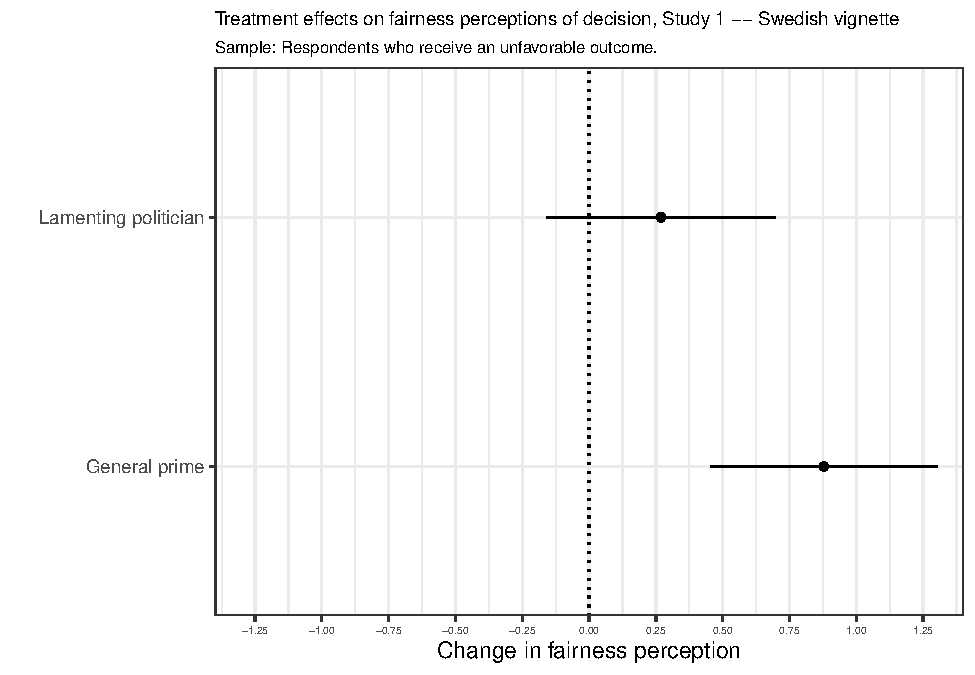
\includegraphics{Goodloser-appendix_files/figure-latex/105_post_fairness-1.pdf}

\begin{Shaded}
\begin{Highlighting}[]
\KeywordTok{ggsave}\NormalTok{(}
  \KeywordTok{here}\NormalTok{(}\StringTok{"output"}\NormalTok{, }\StringTok{"swevig"}\NormalTok{, }\StringTok{"figs"}\NormalTok{, }\StringTok{"pngs"}\NormalTok{, }\StringTok{"exp1-fairness-losers.png"}\NormalTok{),}
  \DataTypeTok{plot =}\NormalTok{ fig,}
  \DataTypeTok{width =} \FloatTok{5.5}\NormalTok{, }\DataTypeTok{height =} \FloatTok{2.75}
\NormalTok{)}

\KeywordTok{ggsave}\NormalTok{(}
  \KeywordTok{here}\NormalTok{(}\StringTok{"output"}\NormalTok{, }\StringTok{"swevig"}\NormalTok{, }\StringTok{"figs"}\NormalTok{, }\StringTok{"pdfs"}\NormalTok{, }\StringTok{"exp1-fairness-losers.pdf"}\NormalTok{),}
  \DataTypeTok{plot =}\NormalTok{ fig,}
  \DataTypeTok{width =} \FloatTok{5.5}\NormalTok{, }\DataTypeTok{height =} \FloatTok{2.75}
\NormalTok{)}


\CommentTok{#Table}
\NormalTok{table <-}\StringTok{ }\NormalTok{res_main }\OperatorTok\StringTok{ }
\StringTok{  }\KeywordTok{select}\NormalTok{(term, estimate, std.error, statistic, p.value) }\OperatorTok\StringTok{ }
\StringTok{  }\KeywordTok{mutate}\NormalTok{(}\DataTypeTok{term =} \KeywordTok{case_when}\NormalTok{( term }\OperatorTok{==}\StringTok{ "(Intercept)"} \OperatorTok{~}\StringTok{ "Not shown"}\NormalTok{,}
\NormalTok{                    term }\OperatorTok{==}\StringTok{ "treatmentLamenting politician"} \OperatorTok{~}\StringTok{ "Lamenting politician"}\NormalTok{,}
\NormalTok{                   term }\OperatorTok{==}\StringTok{ "treatmentGeneral prime"} \OperatorTok{~}\StringTok{ "General prime"}\NormalTok{)}
\NormalTok{         )}

\KeywordTok{kable}\NormalTok{(table, }\DataTypeTok{booktabs =} \OtherTok{TRUE}\NormalTok{, }\DataTypeTok{caption =} \StringTok{"Treatment effects on fairness perceptions of decision, Study 1 -- Swedish vignette"}\NormalTok{, }\DataTypeTok{col.names =} \KeywordTok{linebreak}\NormalTok{(}\KeywordTok{c}\NormalTok{(}\StringTok{"Treatment value"}\NormalTok{, }\StringTok{"Estimate"}\NormalTok{, }\StringTok{"Std. Error"}\NormalTok{, }\StringTok{"t-statistic"}\NormalTok{, }\StringTok{"p value"}\NormalTok{))) }\OperatorTok\StringTok{ }
\StringTok{  }\KeywordTok{kable_styling}\NormalTok{(}\DataTypeTok{bootstrap_options =} \KeywordTok{c}\NormalTok{(}\StringTok{"striped"}\NormalTok{, }\StringTok{"hover"}\NormalTok{, }\StringTok{"responsive"}\NormalTok{)) }
\end{Highlighting}
\end{Shaded}

(\#tab:105\_post\_fairness)Treatment effects on fairness perceptions of
decision, Study 1 -- Swedish vignette

Treatment value

Estimate

Std. Error

t-statistic

p value

Not shown

3.9041096

0.1572271

24.8310160

0.0000000

Lamenting politician

0.1510628

0.2227358

0.6782153

0.4979901

General prime

0.7842021

0.2194461

3.5735530

0.0003909

\section{Justice}\label{justice-1}

\begin{Shaded}
\begin{Highlighting}[]
\NormalTok{res_main <-}\StringTok{  }\KeywordTok{lm}\NormalTok{(justice }\OperatorTok{~}\StringTok{ }\NormalTok{treatment, }\DataTypeTok{data =}\NormalTok{ d) }
\NormalTok{res_main <-}\StringTok{ }\NormalTok{broom}\OperatorTok{::}\KeywordTok{tidy}\NormalTok{(res_main)}

\NormalTok{labels <-}\StringTok{ }\KeywordTok{data.frame}\NormalTok{(}
  \DataTypeTok{term =} \KeywordTok{c}\NormalTok{(}
    \StringTok{"treatmentLamenting politician"}\NormalTok{,}
    \StringTok{"treatmentGeneral prime"}
    
\NormalTok{  ),}
  \DataTypeTok{label =} \KeywordTok{c}\NormalTok{( }\StringTok{"Lamenting politician"}\NormalTok{,}
             \StringTok{"General prime"}\NormalTok{)}
\NormalTok{)}
\CommentTok{#Figure}
\NormalTok{fig <-}\StringTok{   }\NormalTok{res_main }\OperatorTok
\StringTok{  }\KeywordTok{filter}\NormalTok{(term }\OperatorTok{!=}\StringTok{ "(Intercept)"}\NormalTok{) }\OperatorTok\StringTok{ }
\StringTok{  }\KeywordTok{left_join}\NormalTok{(labels, }\DataTypeTok{by =} \StringTok{"term"}\NormalTok{) }\OperatorTok\StringTok{ }
\StringTok{  }
\StringTok{  }\KeywordTok{ggplot}\NormalTok{(}\KeywordTok{aes}\NormalTok{(}\DataTypeTok{x =}\NormalTok{ estimate, }\DataTypeTok{y =}\NormalTok{ label,}
             \DataTypeTok{xmin =}\NormalTok{ estimate }\OperatorTok{-}\StringTok{ }\NormalTok{(}\DecValTok{2} \OperatorTok{*}\StringTok{ }\NormalTok{std.error),}
             \DataTypeTok{xmax =}\NormalTok{ estimate }\OperatorTok{+}\StringTok{ }\NormalTok{(}\DecValTok{2} \OperatorTok{*}\StringTok{ }\NormalTok{std.error))) }\OperatorTok{+}
\StringTok{   }\KeywordTok{geom_errorbarh}\NormalTok{(}\DataTypeTok{height =} \DecValTok{0}\NormalTok{) }\OperatorTok{+}
\StringTok{  }\KeywordTok{geom_point}\NormalTok{() }\OperatorTok{+}
\StringTok{  }\KeywordTok{geom_vline}\NormalTok{(}\KeywordTok{aes}\NormalTok{(}\DataTypeTok{xintercept =} \DecValTok{0}\NormalTok{), }\DataTypeTok{linetype =} \StringTok{"dotted"}\NormalTok{) }\OperatorTok{+}
\StringTok{  }\KeywordTok{scale_x_continuous}\NormalTok{(}\DataTypeTok{limits =} \KeywordTok{c}\NormalTok{(}\OperatorTok{-}\DecValTok{1}\NormalTok{, }\DecValTok{1}\NormalTok{),}
                     \DataTypeTok{breaks =} \KeywordTok{round}\NormalTok{(}\KeywordTok{seq}\NormalTok{(}\OperatorTok{-}\DecValTok{1}\NormalTok{, }\DecValTok{1}\NormalTok{, .}\DecValTok{25}\NormalTok{), }\DecValTok{2}\NormalTok{),}
                     \DataTypeTok{expand =} \KeywordTok{c}\NormalTok{(}\DecValTok{0}\NormalTok{, }\DecValTok{0}\NormalTok{)) }\OperatorTok{+}
\StringTok{  }\KeywordTok{labs}\NormalTok{(}\DataTypeTok{x =} \StringTok{"Change in justice perception"}\NormalTok{,}
       \DataTypeTok{y =} \StringTok{"Decision process attributes"}\NormalTok{) }\OperatorTok{+}
\StringTok{  }\KeywordTok{theme_bw}\NormalTok{() }\OperatorTok{+}
\StringTok{  }\KeywordTok{theme}\NormalTok{(}\DataTypeTok{plot.margin =} \KeywordTok{unit}\NormalTok{(}\KeywordTok{c}\NormalTok{(}\DecValTok{2}\NormalTok{, }\DecValTok{2}\NormalTok{, }\DecValTok{2}\NormalTok{, }\DecValTok{2}\NormalTok{), }\StringTok{"mm"}\NormalTok{), }\DataTypeTok{axis.text.x=}\KeywordTok{element_text}\NormalTok{(}\DataTypeTok{size=}\KeywordTok{rel}\NormalTok{(}\FloatTok{0.6}\NormalTok{))) }\OperatorTok{+}
\StringTok{  }\KeywordTok{theme}\NormalTok{(}\DataTypeTok{panel.spacing =} \KeywordTok{unit}\NormalTok{(}\FloatTok{0.5}\NormalTok{, }\StringTok{"lines"}\NormalTok{))}
\NormalTok{fig}
\end{Highlighting}
\end{Shaded}

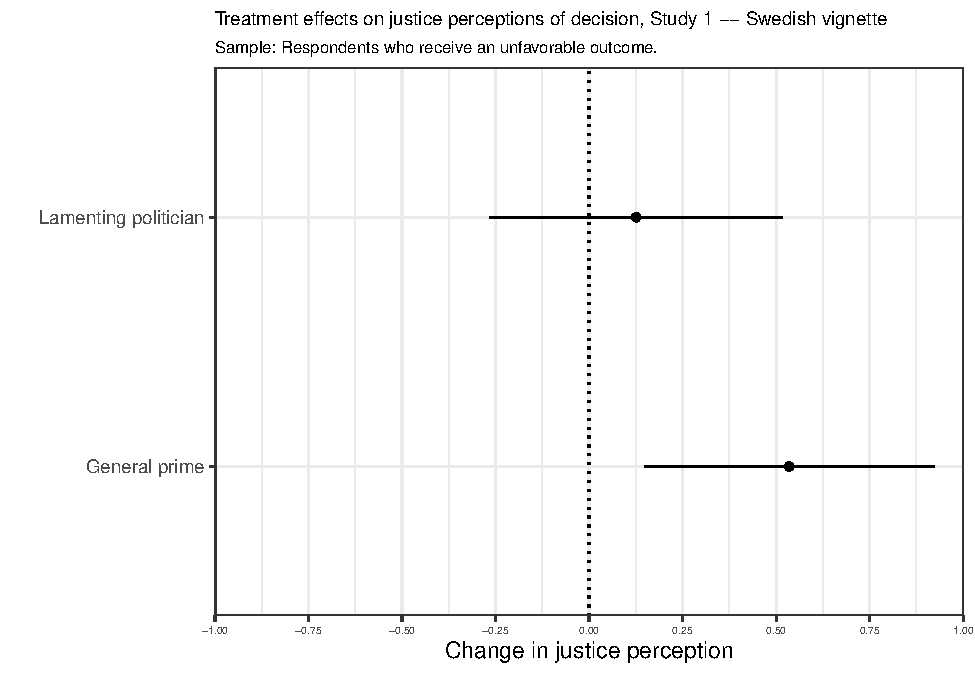
\includegraphics{Goodloser-appendix_files/figure-latex/105_post_justice-1.pdf}

\begin{Shaded}
\begin{Highlighting}[]
\KeywordTok{ggsave}\NormalTok{(}
  \KeywordTok{here}\NormalTok{(}\StringTok{"output"}\NormalTok{, }\StringTok{"swevig"}\NormalTok{, }\StringTok{"figs"}\NormalTok{, }\StringTok{"pngs"}\NormalTok{, }\StringTok{"exp1-justice-losers.png"}\NormalTok{),}
  \DataTypeTok{plot =}\NormalTok{ fig,}
  \DataTypeTok{width =} \FloatTok{5.5}\NormalTok{, }\DataTypeTok{height =} \FloatTok{2.75}
\NormalTok{)}

\KeywordTok{ggsave}\NormalTok{(}
  \KeywordTok{here}\NormalTok{(}\StringTok{"output"}\NormalTok{, }\StringTok{"swevig"}\NormalTok{, }\StringTok{"figs"}\NormalTok{, }\StringTok{"pdfs"}\NormalTok{, }\StringTok{"exp1-justice-losers.pdf"}\NormalTok{),}
  \DataTypeTok{plot =}\NormalTok{ fig,}
  \DataTypeTok{width =} \FloatTok{5.5}\NormalTok{, }\DataTypeTok{height =} \FloatTok{2.75}
\NormalTok{)}


\CommentTok{#Table}
\NormalTok{table <-}\StringTok{ }\NormalTok{res_main }\OperatorTok\StringTok{ }
\StringTok{  }\KeywordTok{select}\NormalTok{(term, estimate, std.error, statistic, p.value) }\OperatorTok\StringTok{ }
\StringTok{  }\KeywordTok{mutate}\NormalTok{(}\DataTypeTok{term =} \KeywordTok{case_when}\NormalTok{( term }\OperatorTok{==}\StringTok{ "(Intercept)"} \OperatorTok{~}\StringTok{ "Not shown"}\NormalTok{,}
\NormalTok{                    term }\OperatorTok{==}\StringTok{ "treatmentLamenting politician"} \OperatorTok{~}\StringTok{ "Lamenting politician"}\NormalTok{,}
\NormalTok{                   term }\OperatorTok{==}\StringTok{ "treatmentGeneral prime"} \OperatorTok{~}\StringTok{ "General prime"}\NormalTok{)}
\NormalTok{         )}

\KeywordTok{kable}\NormalTok{(table, }\DataTypeTok{booktabs =} \OtherTok{TRUE}\NormalTok{, }\DataTypeTok{caption =} \StringTok{"Treatment effects on justice perceptions of decision, Study 1 -- Swedish vignette"}\NormalTok{, }\DataTypeTok{col.names =} \KeywordTok{linebreak}\NormalTok{(}\KeywordTok{c}\NormalTok{(}\StringTok{"Treatment value"}\NormalTok{, }\StringTok{"Estimate"}\NormalTok{, }\StringTok{"Std. Error"}\NormalTok{, }\StringTok{"t-statistic"}\NormalTok{, }\StringTok{"p value"}\NormalTok{))) }\OperatorTok\StringTok{ }
\StringTok{  }\KeywordTok{kable_styling}\NormalTok{(}\DataTypeTok{bootstrap_options =} \KeywordTok{c}\NormalTok{(}\StringTok{"striped"}\NormalTok{, }\StringTok{"hover"}\NormalTok{, }\StringTok{"responsive"}\NormalTok{)) }
\end{Highlighting}
\end{Shaded}

(\#tab:105\_post\_justice)Treatment effects on justice perceptions of
decision, Study 1 -- Swedish vignette

Treatment value

Estimate

Std. Error

t-statistic

p value

Not shown

3.8698630

0.1447119

26.7418457

0.0000000

Lamenting politician

-0.0422768

0.2050061

-0.2062222

0.8367123

General prime

0.5846824

0.2019782

2.8947801

0.0039822

\section{Decision evaluation}\label{decision-evaluation-1}

\begin{Shaded}
\begin{Highlighting}[]
\NormalTok{res_main <-}\StringTok{  }\KeywordTok{lm}\NormalTok{(eval }\OperatorTok{~}\StringTok{ }\NormalTok{treatment, }\DataTypeTok{data =}\NormalTok{ d) }
\NormalTok{res_main <-}\StringTok{ }\NormalTok{broom}\OperatorTok{::}\KeywordTok{tidy}\NormalTok{(res_main)}

\NormalTok{labels <-}\StringTok{ }\KeywordTok{data.frame}\NormalTok{(}
  \DataTypeTok{term =} \KeywordTok{c}\NormalTok{(}
    \StringTok{"treatmentLamenting politician"}\NormalTok{,}
    \StringTok{"treatmentGeneral prime"}
    
\NormalTok{  ),}
  \DataTypeTok{label =} \KeywordTok{c}\NormalTok{( }\StringTok{"Lamenting politician"}\NormalTok{,}
             \StringTok{"General prime"}\NormalTok{)}
\NormalTok{)}
\CommentTok{#Figure}
\NormalTok{fig <-}\StringTok{   }\NormalTok{res_main }\OperatorTok
\StringTok{  }\KeywordTok{filter}\NormalTok{(term }\OperatorTok{!=}\StringTok{ "(Intercept)"}\NormalTok{) }\OperatorTok\StringTok{ }
\StringTok{  }\KeywordTok{left_join}\NormalTok{(labels, }\DataTypeTok{by =} \StringTok{"term"}\NormalTok{) }\OperatorTok\StringTok{ }
\StringTok{  }
\StringTok{  }\KeywordTok{ggplot}\NormalTok{(}\KeywordTok{aes}\NormalTok{(}\DataTypeTok{x =}\NormalTok{ estimate, }\DataTypeTok{y =}\NormalTok{ label,}
             \DataTypeTok{xmin =}\NormalTok{ estimate }\OperatorTok{-}\StringTok{ }\NormalTok{(}\DecValTok{2} \OperatorTok{*}\StringTok{ }\NormalTok{std.error),}
             \DataTypeTok{xmax =}\NormalTok{ estimate }\OperatorTok{+}\StringTok{ }\NormalTok{(}\DecValTok{2} \OperatorTok{*}\StringTok{ }\NormalTok{std.error))) }\OperatorTok{+}
\StringTok{   }\KeywordTok{geom_errorbarh}\NormalTok{(}\DataTypeTok{height =} \DecValTok{0}\NormalTok{) }\OperatorTok{+}
\StringTok{  }\KeywordTok{geom_point}\NormalTok{() }\OperatorTok{+}
\StringTok{  }\KeywordTok{geom_vline}\NormalTok{(}\KeywordTok{aes}\NormalTok{(}\DataTypeTok{xintercept =} \DecValTok{0}\NormalTok{), }\DataTypeTok{linetype =} \StringTok{"dotted"}\NormalTok{) }\OperatorTok{+}
\StringTok{  }\KeywordTok{scale_x_continuous}\NormalTok{(}\DataTypeTok{limits =} \KeywordTok{c}\NormalTok{(}\OperatorTok{-}\DecValTok{1}\NormalTok{, }\DecValTok{1}\NormalTok{),}
                     \DataTypeTok{breaks =} \KeywordTok{round}\NormalTok{(}\KeywordTok{seq}\NormalTok{(}\OperatorTok{-}\DecValTok{1}\NormalTok{, }\DecValTok{1}\NormalTok{, .}\DecValTok{25}\NormalTok{), }\DecValTok{2}\NormalTok{),}
                     \DataTypeTok{expand =} \KeywordTok{c}\NormalTok{(}\DecValTok{0}\NormalTok{, }\DecValTok{0}\NormalTok{)) }\OperatorTok{+}
\StringTok{  }\KeywordTok{labs}\NormalTok{(}\DataTypeTok{x =} \StringTok{"Change in decision evaluation"}\NormalTok{,}
       \DataTypeTok{y =} \StringTok{"Decision process attributes"}\NormalTok{) }\OperatorTok{+}
\StringTok{  }\KeywordTok{theme_bw}\NormalTok{() }\OperatorTok{+}
\StringTok{  }\KeywordTok{theme}\NormalTok{(}\DataTypeTok{plot.margin =} \KeywordTok{unit}\NormalTok{(}\KeywordTok{c}\NormalTok{(}\DecValTok{2}\NormalTok{, }\DecValTok{2}\NormalTok{, }\DecValTok{2}\NormalTok{, }\DecValTok{2}\NormalTok{), }\StringTok{"mm"}\NormalTok{), }\DataTypeTok{axis.text.x=}\KeywordTok{element_text}\NormalTok{(}\DataTypeTok{size=}\KeywordTok{rel}\NormalTok{(}\FloatTok{0.7}\NormalTok{))) }\OperatorTok{+}
\StringTok{  }\KeywordTok{theme}\NormalTok{(}\DataTypeTok{panel.spacing =} \KeywordTok{unit}\NormalTok{(}\FloatTok{0.5}\NormalTok{, }\StringTok{"lines"}\NormalTok{))}
\NormalTok{fig}
\end{Highlighting}
\end{Shaded}

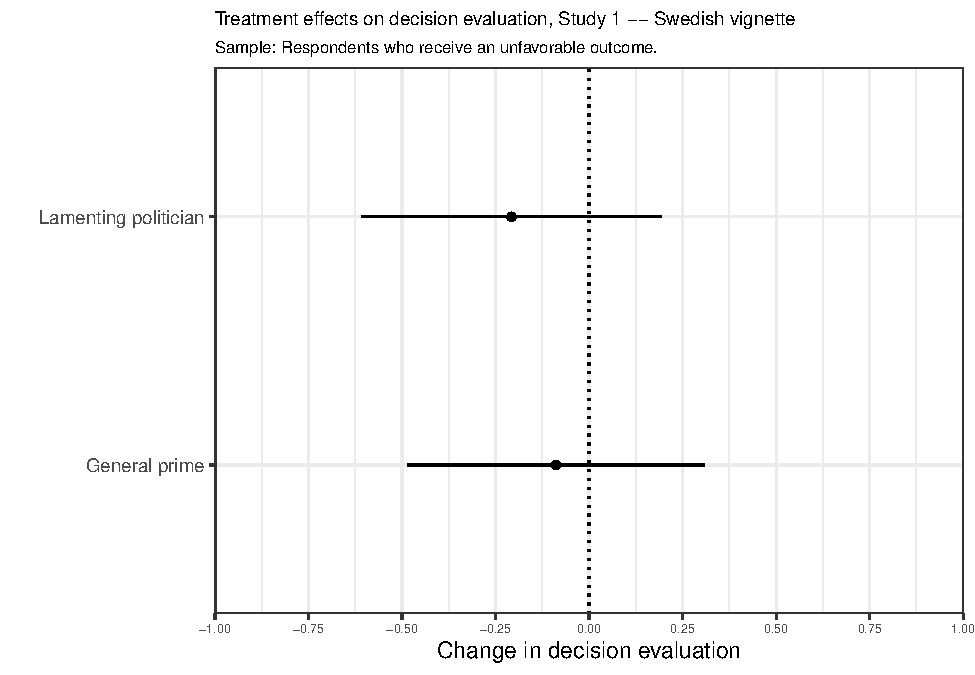
\includegraphics{Goodloser-appendix_files/figure-latex/105_post_eval-1.pdf}

\begin{Shaded}
\begin{Highlighting}[]
\KeywordTok{ggsave}\NormalTok{(}
  \KeywordTok{here}\NormalTok{(}\StringTok{"output"}\NormalTok{, }\StringTok{"swevig"}\NormalTok{, }\StringTok{"figs"}\NormalTok{, }\StringTok{"pngs"}\NormalTok{, }\StringTok{"exp1-eval-losers.png"}\NormalTok{),}
  \DataTypeTok{plot =}\NormalTok{ fig,}
  \DataTypeTok{width =} \FloatTok{5.5}\NormalTok{, }\DataTypeTok{height =} \FloatTok{2.75}
\NormalTok{)}

\KeywordTok{ggsave}\NormalTok{(}
  \KeywordTok{here}\NormalTok{(}\StringTok{"output"}\NormalTok{, }\StringTok{"swevig"}\NormalTok{, }\StringTok{"figs"}\NormalTok{, }\StringTok{"pdfs"}\NormalTok{, }\StringTok{"exp1-eval-losers.pdf"}\NormalTok{),}
  \DataTypeTok{plot =}\NormalTok{ fig,}
  \DataTypeTok{width =} \FloatTok{5.5}\NormalTok{, }\DataTypeTok{height =} \FloatTok{2.75}
\NormalTok{)}


\CommentTok{#Table}
\NormalTok{table <-}\StringTok{ }\NormalTok{res_main }\OperatorTok\StringTok{ }
\StringTok{  }\KeywordTok{select}\NormalTok{(term, estimate, std.error, statistic, p.value) }\OperatorTok\StringTok{ }
\StringTok{  }\KeywordTok{mutate}\NormalTok{(}\DataTypeTok{term =} \KeywordTok{case_when}\NormalTok{( term }\OperatorTok{==}\StringTok{ "(Intercept)"} \OperatorTok{~}\StringTok{ "Not shown"}\NormalTok{,}
\NormalTok{                    term }\OperatorTok{==}\StringTok{ "treatmentLamenting politician"} \OperatorTok{~}\StringTok{ "Lamenting politician"}\NormalTok{,}
\NormalTok{                   term }\OperatorTok{==}\StringTok{ "treatmentGeneral prime"} \OperatorTok{~}\StringTok{ "General prime"}\NormalTok{)}
\NormalTok{         )}

\KeywordTok{kable}\NormalTok{(table, }\DataTypeTok{booktabs =} \OtherTok{TRUE}\NormalTok{, }\DataTypeTok{caption =} \StringTok{"Treatment effects on decision evaluation, Study 1 -- Swedish vignette"}\NormalTok{, }\DataTypeTok{col.names =} \KeywordTok{linebreak}\NormalTok{(}\KeywordTok{c}\NormalTok{(}\StringTok{"Treatment value"}\NormalTok{, }\StringTok{"Estimate"}\NormalTok{, }\StringTok{"Std. Error"}\NormalTok{, }\StringTok{"t-statistic"}\NormalTok{, }\StringTok{"p value"}\NormalTok{))) }\OperatorTok\StringTok{ }
\StringTok{  }\KeywordTok{kable_styling}\NormalTok{(}\DataTypeTok{bootstrap_options =} \KeywordTok{c}\NormalTok{(}\StringTok{"striped"}\NormalTok{, }\StringTok{"hover"}\NormalTok{, }\StringTok{"responsive"}\NormalTok{)) }
\end{Highlighting}
\end{Shaded}

(\#tab:105\_post\_eval)Treatment effects on decision evaluation, Study 1
-- Swedish vignette

Treatment value

Estimate

Std. Error

t-statistic

p value

Not shown

4.0547945

0.1769636

22.9131510

0.0000000

Lamenting politician

-0.0616911

0.2506955

-0.2460797

0.8057348

General prime

-0.1586906

0.2469928

-0.6424909

0.5208876

\section{Willingness to accept}\label{willingness-to-accept-1}

\begin{Shaded}
\begin{Highlighting}[]
\NormalTok{res_main <-}\StringTok{  }\KeywordTok{lm}\NormalTok{(accept }\OperatorTok{~}\StringTok{ }\NormalTok{treatment, }\DataTypeTok{data =}\NormalTok{ d) }
\NormalTok{res_main <-}\StringTok{ }\NormalTok{broom}\OperatorTok{::}\KeywordTok{tidy}\NormalTok{(res_main)}

\NormalTok{labels <-}\StringTok{ }\KeywordTok{data.frame}\NormalTok{(}
  \DataTypeTok{term =} \KeywordTok{c}\NormalTok{(}
    \StringTok{"treatmentLamenting politician"}\NormalTok{,}
    \StringTok{"treatmentGeneral prime"}
    
\NormalTok{  ),}
  \DataTypeTok{label =} \KeywordTok{c}\NormalTok{( }\StringTok{"Lamenting politician"}\NormalTok{,}
             \StringTok{"General prime"}\NormalTok{)}
\NormalTok{)}
\CommentTok{#Figure}
\NormalTok{fig <-}\StringTok{   }\NormalTok{res_main }\OperatorTok
\StringTok{  }\KeywordTok{filter}\NormalTok{(term }\OperatorTok{!=}\StringTok{ "(Intercept)"}\NormalTok{) }\OperatorTok\StringTok{ }
\StringTok{  }\KeywordTok{left_join}\NormalTok{(labels, }\DataTypeTok{by =} \StringTok{"term"}\NormalTok{) }\OperatorTok\StringTok{ }
\StringTok{  }
\StringTok{  }\KeywordTok{ggplot}\NormalTok{(}\KeywordTok{aes}\NormalTok{(}\DataTypeTok{x =}\NormalTok{ estimate, }\DataTypeTok{y =}\NormalTok{ label,}
             \DataTypeTok{xmin =}\NormalTok{ estimate }\OperatorTok{-}\StringTok{ }\NormalTok{(}\DecValTok{2} \OperatorTok{*}\StringTok{ }\NormalTok{std.error),}
             \DataTypeTok{xmax =}\NormalTok{ estimate }\OperatorTok{+}\StringTok{ }\NormalTok{(}\DecValTok{2} \OperatorTok{*}\StringTok{ }\NormalTok{std.error))) }\OperatorTok{+}
\StringTok{   }\KeywordTok{geom_errorbarh}\NormalTok{(}\DataTypeTok{height =} \DecValTok{0}\NormalTok{) }\OperatorTok{+}
\StringTok{  }\KeywordTok{geom_point}\NormalTok{() }\OperatorTok{+}
\StringTok{  }\KeywordTok{geom_vline}\NormalTok{(}\KeywordTok{aes}\NormalTok{(}\DataTypeTok{xintercept =} \DecValTok{0}\NormalTok{), }\DataTypeTok{linetype =} \StringTok{"dotted"}\NormalTok{) }\OperatorTok{+}
\StringTok{  }\KeywordTok{scale_x_continuous}\NormalTok{(}\DataTypeTok{limits =} \KeywordTok{c}\NormalTok{(}\OperatorTok{-}\DecValTok{1}\NormalTok{, }\DecValTok{1}\NormalTok{),}
                     \DataTypeTok{breaks =} \KeywordTok{round}\NormalTok{(}\KeywordTok{seq}\NormalTok{(}\OperatorTok{-}\DecValTok{1}\NormalTok{, }\DecValTok{1}\NormalTok{, .}\DecValTok{25}\NormalTok{), }\DecValTok{2}\NormalTok{),}
                     \DataTypeTok{expand =} \KeywordTok{c}\NormalTok{(}\DecValTok{0}\NormalTok{, }\DecValTok{0}\NormalTok{)) }\OperatorTok{+}
\StringTok{  }\KeywordTok{labs}\NormalTok{(}\DataTypeTok{x =} \StringTok{"Change in willingness to accept outcome"}\NormalTok{,}
       \DataTypeTok{y =} \StringTok{"Decision process attributes"}\NormalTok{) }\OperatorTok{+}
\StringTok{  }\KeywordTok{theme_bw}\NormalTok{() }\OperatorTok{+}
\StringTok{  }\KeywordTok{theme}\NormalTok{(}\DataTypeTok{plot.margin =} \KeywordTok{unit}\NormalTok{(}\KeywordTok{c}\NormalTok{(}\DecValTok{2}\NormalTok{, }\DecValTok{2}\NormalTok{, }\DecValTok{2}\NormalTok{, }\DecValTok{2}\NormalTok{), }\StringTok{"mm"}\NormalTok{), }\DataTypeTok{axis.text.x=}\KeywordTok{element_text}\NormalTok{(}\DataTypeTok{size=}\KeywordTok{rel}\NormalTok{(}\FloatTok{0.6}\NormalTok{))) }\OperatorTok{+}
\StringTok{  }\KeywordTok{theme}\NormalTok{(}\DataTypeTok{panel.spacing =} \KeywordTok{unit}\NormalTok{(}\FloatTok{0.5}\NormalTok{, }\StringTok{"lines"}\NormalTok{))}
\NormalTok{fig}
\end{Highlighting}
\end{Shaded}

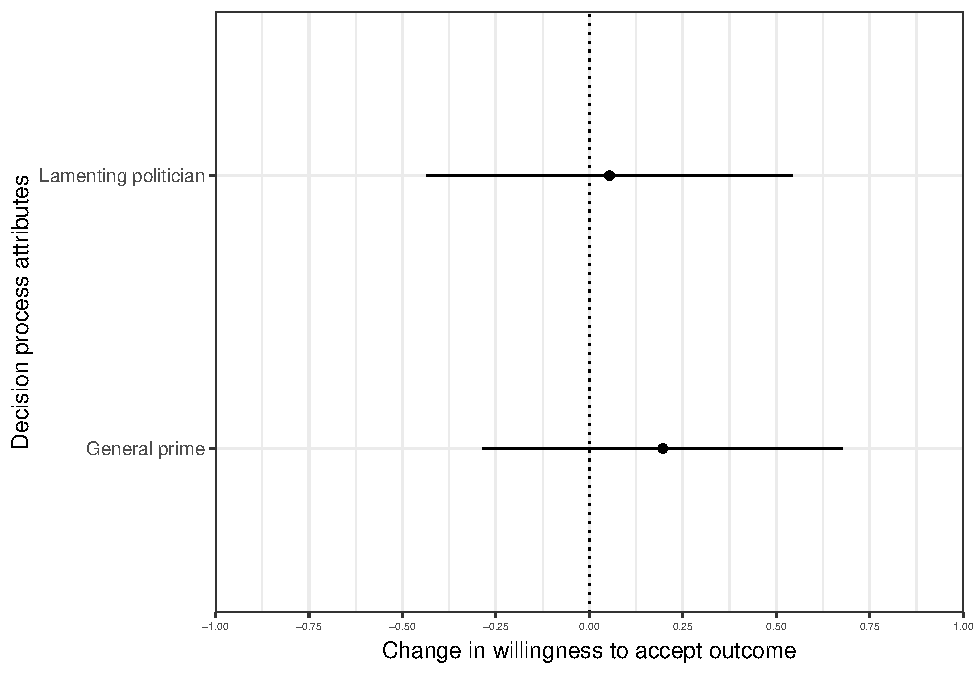
\includegraphics{Goodloser-appendix_files/figure-latex/105_post_accept-1.pdf}

\begin{Shaded}
\begin{Highlighting}[]
\KeywordTok{ggsave}\NormalTok{(}
  \KeywordTok{here}\NormalTok{(}\StringTok{"output"}\NormalTok{, }\StringTok{"swevig"}\NormalTok{, }\StringTok{"figs"}\NormalTok{, }\StringTok{"pngs"}\NormalTok{, }\StringTok{"exp1-accept-losers.png"}\NormalTok{),}
  \DataTypeTok{plot =}\NormalTok{ fig,}
  \DataTypeTok{width =} \FloatTok{5.5}\NormalTok{, }\DataTypeTok{height =} \FloatTok{2.75}
\NormalTok{)}

\KeywordTok{ggsave}\NormalTok{(}
  \KeywordTok{here}\NormalTok{(}\StringTok{"output"}\NormalTok{, }\StringTok{"swevig"}\NormalTok{, }\StringTok{"figs"}\NormalTok{, }\StringTok{"pdfs"}\NormalTok{, }\StringTok{"exp1-accept-losers.pdf"}\NormalTok{),}
  \DataTypeTok{plot =}\NormalTok{ fig,}
  \DataTypeTok{width =} \FloatTok{5.5}\NormalTok{, }\DataTypeTok{height =} \FloatTok{2.75}
\NormalTok{)}


\CommentTok{#Table}
\NormalTok{table <-}\StringTok{ }\NormalTok{res_main }\OperatorTok\StringTok{ }
\StringTok{  }\KeywordTok{select}\NormalTok{(term, estimate, std.error, statistic, p.value) }\OperatorTok\StringTok{ }
\StringTok{  }\KeywordTok{mutate}\NormalTok{(}\DataTypeTok{term =} \KeywordTok{case_when}\NormalTok{( term }\OperatorTok{==}\StringTok{ "(Intercept)"} \OperatorTok{~}\StringTok{ "Not shown"}\NormalTok{,}
\NormalTok{                    term }\OperatorTok{==}\StringTok{ "treatmentLamenting politician"} \OperatorTok{~}\StringTok{ "Lamenting politician"}\NormalTok{,}
\NormalTok{                   term }\OperatorTok{==}\StringTok{ "treatmentGeneral prime"} \OperatorTok{~}\StringTok{ "General prime"}\NormalTok{)}
\NormalTok{         )}

\KeywordTok{kable}\NormalTok{(table, }\DataTypeTok{booktabs =} \OtherTok{TRUE}\NormalTok{, }\DataTypeTok{caption =} \StringTok{"Treatment effects on willingness to accept decision, Study 1 -- Swedish vignette"}\NormalTok{, }\DataTypeTok{col.names =} \KeywordTok{linebreak}\NormalTok{(}\KeywordTok{c}\NormalTok{(}\StringTok{"Treatment value"}\NormalTok{, }\StringTok{"Estimate"}\NormalTok{, }\StringTok{"Std. Error"}\NormalTok{, }\StringTok{"t-statistic"}\NormalTok{, }\StringTok{"p value"}\NormalTok{))) }\OperatorTok\StringTok{ }
\StringTok{  }\KeywordTok{kable_styling}\NormalTok{(}\DataTypeTok{bootstrap_options =} \KeywordTok{c}\NormalTok{(}\StringTok{"striped"}\NormalTok{, }\StringTok{"hover"}\NormalTok{, }\StringTok{"responsive"}\NormalTok{)) }
\end{Highlighting}
\end{Shaded}

(\#tab:105\_post\_accept)Treatment effects on willingness to accept
decision, Study 1 -- Swedish vignette

Treatment value

Estimate

Std. Error

t-statistic

p value

Not shown

4.8356164

0.1724504

28.0406164

0.0000000

Lamenting politician

0.0540387

0.2443019

0.2211966

0.8250415

General prime

0.1968511

0.2406936

0.8178493

0.4138839

\section{Compliance}\label{compliance-1}

\begin{Shaded}
\begin{Highlighting}[]
\NormalTok{res_main <-}\StringTok{  }\KeywordTok{lm}\NormalTok{(comply }\OperatorTok{~}\StringTok{ }\NormalTok{treatment, }\DataTypeTok{data =}\NormalTok{ d) }
\NormalTok{res_main <-}\StringTok{ }\NormalTok{broom}\OperatorTok{::}\KeywordTok{tidy}\NormalTok{(res_main)}

\NormalTok{labels <-}\StringTok{ }\KeywordTok{data.frame}\NormalTok{(}
  \DataTypeTok{term =} \KeywordTok{c}\NormalTok{(}
    \StringTok{"treatmentLamenting politician"}\NormalTok{,}
    \StringTok{"treatmentGeneral prime"}
    
\NormalTok{  ),}
  \DataTypeTok{label =} \KeywordTok{c}\NormalTok{( }\StringTok{"Lamenting politician"}\NormalTok{,}
             \StringTok{"General prime"}\NormalTok{)}
\NormalTok{)}
\CommentTok{#Figure}
\NormalTok{fig <-}\StringTok{   }\NormalTok{res_main }\OperatorTok
\StringTok{  }\KeywordTok{filter}\NormalTok{(term }\OperatorTok{!=}\StringTok{ "(Intercept)"}\NormalTok{) }\OperatorTok\StringTok{ }
\StringTok{  }\KeywordTok{left_join}\NormalTok{(labels, }\DataTypeTok{by =} \StringTok{"term"}\NormalTok{) }\OperatorTok\StringTok{ }
\StringTok{  }
\StringTok{  }\KeywordTok{ggplot}\NormalTok{(}\KeywordTok{aes}\NormalTok{(}\DataTypeTok{x =}\NormalTok{ estimate, }\DataTypeTok{y =}\NormalTok{ label,}
             \DataTypeTok{xmin =}\NormalTok{ estimate }\OperatorTok{-}\StringTok{ }\NormalTok{(}\DecValTok{2} \OperatorTok{*}\StringTok{ }\NormalTok{std.error),}
             \DataTypeTok{xmax =}\NormalTok{ estimate }\OperatorTok{+}\StringTok{ }\NormalTok{(}\DecValTok{2} \OperatorTok{*}\StringTok{ }\NormalTok{std.error))) }\OperatorTok{+}
\StringTok{   }\KeywordTok{geom_errorbarh}\NormalTok{(}\DataTypeTok{height =} \DecValTok{0}\NormalTok{) }\OperatorTok{+}
\StringTok{  }\KeywordTok{geom_point}\NormalTok{() }\OperatorTok{+}
\StringTok{  }\KeywordTok{geom_vline}\NormalTok{(}\KeywordTok{aes}\NormalTok{(}\DataTypeTok{xintercept =} \DecValTok{0}\NormalTok{), }\DataTypeTok{linetype =} \StringTok{"dotted"}\NormalTok{) }\OperatorTok{+}
\StringTok{  }\KeywordTok{scale_x_continuous}\NormalTok{(}\DataTypeTok{limits =} \KeywordTok{c}\NormalTok{(}\OperatorTok{-}\DecValTok{1}\NormalTok{, }\DecValTok{1}\NormalTok{),}
                     \DataTypeTok{breaks =} \KeywordTok{round}\NormalTok{(}\KeywordTok{seq}\NormalTok{(}\OperatorTok{-}\DecValTok{1}\NormalTok{, }\DecValTok{1}\NormalTok{, .}\DecValTok{25}\NormalTok{), }\DecValTok{2}\NormalTok{),}
                     \DataTypeTok{expand =} \KeywordTok{c}\NormalTok{(}\DecValTok{0}\NormalTok{, }\DecValTok{0}\NormalTok{)) }\OperatorTok{+}
\StringTok{  }\KeywordTok{labs}\NormalTok{(}\DataTypeTok{x =} \StringTok{"Change in decision compliance"}\NormalTok{,}
       \DataTypeTok{y =} \StringTok{"Decision process attributes"}\NormalTok{) }\OperatorTok{+}
\StringTok{  }\KeywordTok{theme_bw}\NormalTok{() }\OperatorTok{+}
\StringTok{  }\KeywordTok{theme}\NormalTok{(}\DataTypeTok{plot.margin =} \KeywordTok{unit}\NormalTok{(}\KeywordTok{c}\NormalTok{(}\DecValTok{2}\NormalTok{, }\DecValTok{2}\NormalTok{, }\DecValTok{2}\NormalTok{, }\DecValTok{2}\NormalTok{), }\StringTok{"mm"}\NormalTok{), }\DataTypeTok{axis.text.x=}\KeywordTok{element_text}\NormalTok{(}\DataTypeTok{size=}\KeywordTok{rel}\NormalTok{(}\FloatTok{0.6}\NormalTok{))) }\OperatorTok{+}
\StringTok{  }\KeywordTok{theme}\NormalTok{(}\DataTypeTok{panel.spacing =} \KeywordTok{unit}\NormalTok{(}\FloatTok{0.5}\NormalTok{, }\StringTok{"lines"}\NormalTok{))}
\NormalTok{fig}
\end{Highlighting}
\end{Shaded}

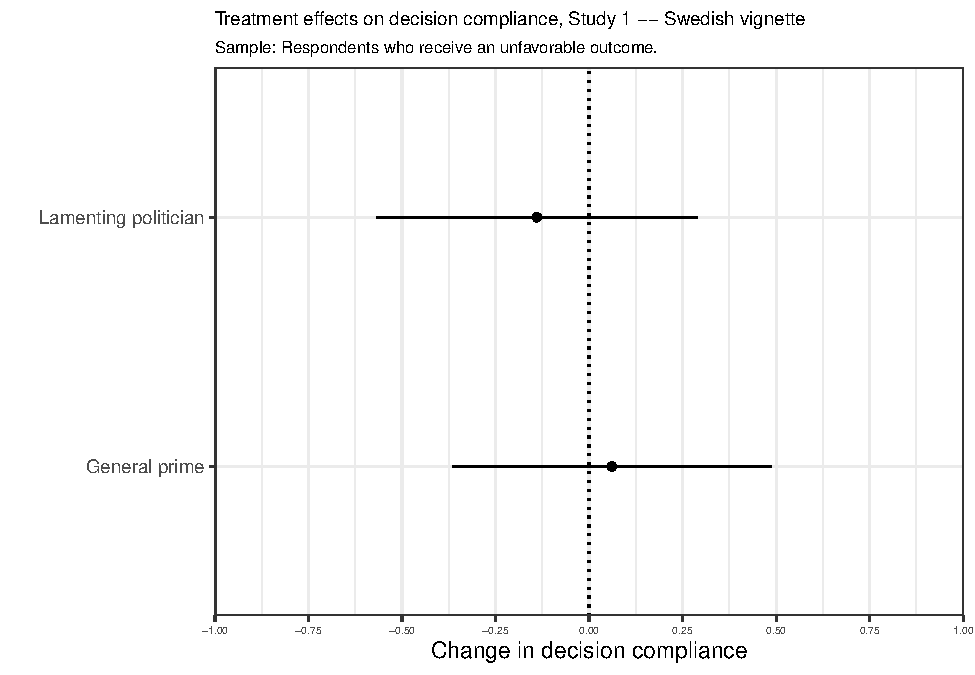
\includegraphics{Goodloser-appendix_files/figure-latex/105_post_comply-1.pdf}

\begin{Shaded}
\begin{Highlighting}[]
\KeywordTok{ggsave}\NormalTok{(}
  \KeywordTok{here}\NormalTok{(}\StringTok{"output"}\NormalTok{, }\StringTok{"swevig"}\NormalTok{, }\StringTok{"figs"}\NormalTok{, }\StringTok{"pngs"}\NormalTok{, }\StringTok{"exp1-comply-losers.png"}\NormalTok{),}
  \DataTypeTok{plot =}\NormalTok{ fig,}
  \DataTypeTok{width =} \FloatTok{5.5}\NormalTok{, }\DataTypeTok{height =} \FloatTok{2.75}
\NormalTok{)}

\KeywordTok{ggsave}\NormalTok{(}
  \KeywordTok{here}\NormalTok{(}\StringTok{"output"}\NormalTok{, }\StringTok{"swevig"}\NormalTok{, }\StringTok{"figs"}\NormalTok{, }\StringTok{"pdfs"}\NormalTok{, }\StringTok{"exp1-comply-losers.pdf"}\NormalTok{),}
  \DataTypeTok{plot =}\NormalTok{ fig,}
  \DataTypeTok{width =} \FloatTok{5.5}\NormalTok{, }\DataTypeTok{height =} \FloatTok{2.75}
\NormalTok{)}


\CommentTok{#Table}
\NormalTok{table <-}\StringTok{ }\NormalTok{res_main }\OperatorTok\StringTok{ }
\StringTok{  }\KeywordTok{select}\NormalTok{(term, estimate, std.error, statistic, p.value) }\OperatorTok\StringTok{ }
\StringTok{  }\KeywordTok{mutate}\NormalTok{(}\DataTypeTok{term =} \KeywordTok{case_when}\NormalTok{( term }\OperatorTok{==}\StringTok{ "(Intercept)"} \OperatorTok{~}\StringTok{ "Not shown"}\NormalTok{,}
\NormalTok{                    term }\OperatorTok{==}\StringTok{ "treatmentLamenting politician"} \OperatorTok{~}\StringTok{ "Lamenting politician"}\NormalTok{,}
\NormalTok{                   term }\OperatorTok{==}\StringTok{ "treatmentGeneral prime"} \OperatorTok{~}\StringTok{ "General prime"}\NormalTok{)}
\NormalTok{         )}

\KeywordTok{kable}\NormalTok{(table, }\DataTypeTok{booktabs =} \OtherTok{TRUE}\NormalTok{, }\DataTypeTok{caption =} \StringTok{"Treatment effects on decision compliance, Study 1 -- Swedish vignette"}\NormalTok{, }\DataTypeTok{col.names =} \KeywordTok{linebreak}\NormalTok{(}\KeywordTok{c}\NormalTok{(}\StringTok{"Treatment value"}\NormalTok{, }\StringTok{"Estimate"}\NormalTok{, }\StringTok{"Std. Error"}\NormalTok{, }\StringTok{"t-statistic"}\NormalTok{, }\StringTok{"p value"}\NormalTok{))) }\OperatorTok\StringTok{ }
\StringTok{  }\KeywordTok{kable_styling}\NormalTok{(}\DataTypeTok{bootstrap_options =} \KeywordTok{c}\NormalTok{(}\StringTok{"striped"}\NormalTok{, }\StringTok{"hover"}\NormalTok{, }\StringTok{"responsive"}\NormalTok{)) }
\end{Highlighting}
\end{Shaded}

(\#tab:105\_post\_comply)Treatment effects on decision compliance, Study
1 -- Swedish vignette

Treatment value

Estimate

Std. Error

t-statistic

p value

Not shown

4.8082192

0.1618013

29.7168094

0.0000000

Lamenting politician

0.0469532

0.2292158

0.2048429

0.8377891

General prime

0.2242484

0.2258304

0.9929947

0.3212558

\chapter{Effects on winners}\label{effects-on-winners}

\begin{Shaded}
\begin{Highlighting}[]
\ControlFlowTok{if}\NormalTok{(}\OperatorTok{!}\KeywordTok{require}\NormalTok{(}\StringTok{"broom"}\NormalTok{))\{}\KeywordTok{install.packages}\NormalTok{(}\StringTok{"broom"}\NormalTok{);  }\KeywordTok{library}\NormalTok{(broom)\}}
\ControlFlowTok{if}\NormalTok{(}\OperatorTok{!}\KeywordTok{require}\NormalTok{(}\StringTok{"haven"}\NormalTok{))\{}\KeywordTok{install.packages}\NormalTok{(}\StringTok{"haven"}\NormalTok{);  }\KeywordTok{library}\NormalTok{(haven)\}}
\ControlFlowTok{if}\NormalTok{(}\OperatorTok{!}\KeywordTok{require}\NormalTok{(}\StringTok{"here"}\NormalTok{))\{}\KeywordTok{install.packages}\NormalTok{(}\StringTok{"here"}\NormalTok{);  }\KeywordTok{library}\NormalTok{(here)\}}
\ControlFlowTok{if}\NormalTok{(}\OperatorTok{!}\KeywordTok{require}\NormalTok{(}\StringTok{"knitr"}\NormalTok{))\{}\KeywordTok{install.packages}\NormalTok{(}\StringTok{"knitr"}\NormalTok{);  }\KeywordTok{library}\NormalTok{(knitr)\}}
\KeywordTok{options}\NormalTok{(}\DataTypeTok{kableExtra.latex.load_packages =} \OtherTok{FALSE}\NormalTok{) }
\ControlFlowTok{if}\NormalTok{(}\OperatorTok{!}\KeywordTok{require}\NormalTok{(}\StringTok{"kableExtra"}\NormalTok{))\{}\KeywordTok{install.packages}\NormalTok{(}\StringTok{"kableExtra"}\NormalTok{);  }\KeywordTok{library}\NormalTok{(kableExtra)\}}
\ControlFlowTok{if}\NormalTok{(}\OperatorTok{!}\KeywordTok{require}\NormalTok{(}\StringTok{"naniar"}\NormalTok{))\{}\KeywordTok{install.packages}\NormalTok{(}\StringTok{"naniar"}\NormalTok{);  }\KeywordTok{library}\NormalTok{(naniar)\}}
\ControlFlowTok{if}\NormalTok{(}\OperatorTok{!}\KeywordTok{require}\NormalTok{(}\StringTok{"tidyverse"}\NormalTok{))\{}\KeywordTok{install.packages}\NormalTok{(}\StringTok{"tidyverse"}\NormalTok{);  }\KeywordTok{library}\NormalTok{(tidyverse)\}}
\CommentTok{# The analysis uses custom functions included in the compendium. Install the included pkg with `devtools::install()` or just install from github with:}
\ControlFlowTok{if}\NormalTok{ (}\OperatorTok{!}\KeywordTok{require}\NormalTok{(wiggle)) \{  devtools}\OperatorTok{::}\KeywordTok{install_github}\NormalTok{(}\StringTok{"mikajoh/wiggle"}\NormalTok{)\}}

\KeywordTok{set.seed}\NormalTok{(}\DecValTok{2016}\NormalTok{)}
\NormalTok{## Utils. }
\KeywordTok{source}\NormalTok{(}\StringTok{"goodloser-utils.R"}\NormalTok{)}

\NormalTok{d <-}\StringTok{ }\KeywordTok{read_sav}\NormalTok{(}\StringTok{"Data/Goodloser-exp1.sav"}\NormalTok{)}

\NormalTok{knitr}\OperatorTok{::}\NormalTok{opts_chunk}\OperatorTok{$}\KeywordTok{set}\NormalTok{(}\DataTypeTok{echo =} \OtherTok{TRUE}\NormalTok{, }\DataTypeTok{knitr.kable.NA =} \StringTok{""}\NormalTok{, }\DataTypeTok{cache =} \OtherTok{FALSE}\NormalTok{, }\DataTypeTok{warning =} \OtherTok{FALSE}\NormalTok{)}
\end{Highlighting}
\end{Shaded}

\section{Prepare data}\label{prepare-data-2}

Select only respondents who receive a favorable outcome

\begin{Shaded}
\begin{Highlighting}[]
\NormalTok{d <-}\StringTok{ }\NormalTok{d }\OperatorTok\StringTok{ }
\StringTok{  }\KeywordTok{filter}\NormalTok{(favorability }\OperatorTok{==}\StringTok{ "Favorable"}\NormalTok{) }\OperatorTok\StringTok{ }
\StringTok{  }\KeywordTok{mutate}\NormalTok{(}\DataTypeTok{treatment =} \KeywordTok{lvls_reorder}\NormalTok{(treatment, }\KeywordTok{c}\NormalTok{(}\DecValTok{3}\NormalTok{, }\DecValTok{2}\NormalTok{, }\DecValTok{1}\NormalTok{)))}
\end{Highlighting}
\end{Shaded}

\section{Fairness}\label{fairness-2}

\begin{Shaded}
\begin{Highlighting}[]
\NormalTok{res_main <-}\StringTok{  }\KeywordTok{lm}\NormalTok{(fairness }\OperatorTok{~}\StringTok{ }\NormalTok{treatment, }\DataTypeTok{data =}\NormalTok{ d) }
\NormalTok{res_main <-}\StringTok{ }\NormalTok{broom}\OperatorTok{::}\KeywordTok{tidy}\NormalTok{(res_main)}

\NormalTok{labels <-}\StringTok{ }\KeywordTok{data.frame}\NormalTok{(}
  \DataTypeTok{term =} \KeywordTok{c}\NormalTok{(}
    \StringTok{"treatmentLamenting politician"}\NormalTok{,}
    \StringTok{"treatmentGeneral prime"}
    
\NormalTok{  ),}
  \DataTypeTok{label =} \KeywordTok{c}\NormalTok{( }\StringTok{"Lamenting politician"}\NormalTok{,}
             \StringTok{"General prime"}\NormalTok{)}
\NormalTok{)}
\CommentTok{#Figure}
\NormalTok{fig <-}\StringTok{   }\NormalTok{res_main }\OperatorTok
\StringTok{  }\KeywordTok{filter}\NormalTok{(term }\OperatorTok{!=}\StringTok{ "(Intercept)"}\NormalTok{) }\OperatorTok\StringTok{ }
\StringTok{  }\KeywordTok{left_join}\NormalTok{(labels, }\DataTypeTok{by =} \StringTok{"term"}\NormalTok{) }\OperatorTok\StringTok{ }
\StringTok{  }
\StringTok{  }\KeywordTok{ggplot}\NormalTok{(}\KeywordTok{aes}\NormalTok{(}\DataTypeTok{x =}\NormalTok{ estimate, }\DataTypeTok{y =}\NormalTok{ label,}
             \DataTypeTok{xmin =}\NormalTok{ estimate }\OperatorTok{-}\StringTok{ }\NormalTok{(}\DecValTok{2} \OperatorTok{*}\StringTok{ }\NormalTok{std.error),}
             \DataTypeTok{xmax =}\NormalTok{ estimate }\OperatorTok{+}\StringTok{ }\NormalTok{(}\DecValTok{2} \OperatorTok{*}\StringTok{ }\NormalTok{std.error))) }\OperatorTok{+}
\StringTok{   }\KeywordTok{geom_errorbarh}\NormalTok{(}\DataTypeTok{height =} \DecValTok{0}\NormalTok{) }\OperatorTok{+}
\StringTok{  }\KeywordTok{geom_point}\NormalTok{() }\OperatorTok{+}
\StringTok{  }\KeywordTok{geom_vline}\NormalTok{(}\KeywordTok{aes}\NormalTok{(}\DataTypeTok{xintercept =} \DecValTok{0}\NormalTok{), }\DataTypeTok{linetype =} \StringTok{"dotted"}\NormalTok{) }\OperatorTok{+}
\StringTok{  }\KeywordTok{scale_x_continuous}\NormalTok{(}\DataTypeTok{limits =} \KeywordTok{c}\NormalTok{(}\OperatorTok{-}\FloatTok{1.3}\NormalTok{, }\FloatTok{1.3}\NormalTok{),}
                     \DataTypeTok{breaks =} \KeywordTok{round}\NormalTok{(}\KeywordTok{seq}\NormalTok{(}\OperatorTok{-}\DecValTok{1}\NormalTok{, }\DecValTok{1}\NormalTok{, .}\DecValTok{25}\NormalTok{), }\DecValTok{2}\NormalTok{),}
                     \DataTypeTok{expand =} \KeywordTok{c}\NormalTok{(}\DecValTok{0}\NormalTok{, }\DecValTok{0}\NormalTok{)) }\OperatorTok{+}
\StringTok{  }\KeywordTok{labs}\NormalTok{(}\DataTypeTok{x =} \StringTok{"Change in fairness perception"}\NormalTok{,}
       \DataTypeTok{y =} \StringTok{"Decision process attributes"}\NormalTok{) }\OperatorTok{+}
\StringTok{  }\KeywordTok{theme_bw}\NormalTok{() }\OperatorTok{+}
\StringTok{  }\KeywordTok{theme}\NormalTok{(}\DataTypeTok{plot.margin =} \KeywordTok{unit}\NormalTok{(}\KeywordTok{c}\NormalTok{(}\DecValTok{2}\NormalTok{, }\DecValTok{2}\NormalTok{, }\DecValTok{2}\NormalTok{, }\DecValTok{2}\NormalTok{), }\StringTok{"mm"}\NormalTok{), }\DataTypeTok{axis.text.x=}\KeywordTok{element_text}\NormalTok{(}\DataTypeTok{size=}\KeywordTok{rel}\NormalTok{(}\FloatTok{0.6}\NormalTok{))) }\OperatorTok{+}
\StringTok{  }\KeywordTok{theme}\NormalTok{(}\DataTypeTok{panel.spacing =} \KeywordTok{unit}\NormalTok{(}\FloatTok{0.5}\NormalTok{, }\StringTok{"lines"}\NormalTok{))}
\NormalTok{fig}
\end{Highlighting}
\end{Shaded}

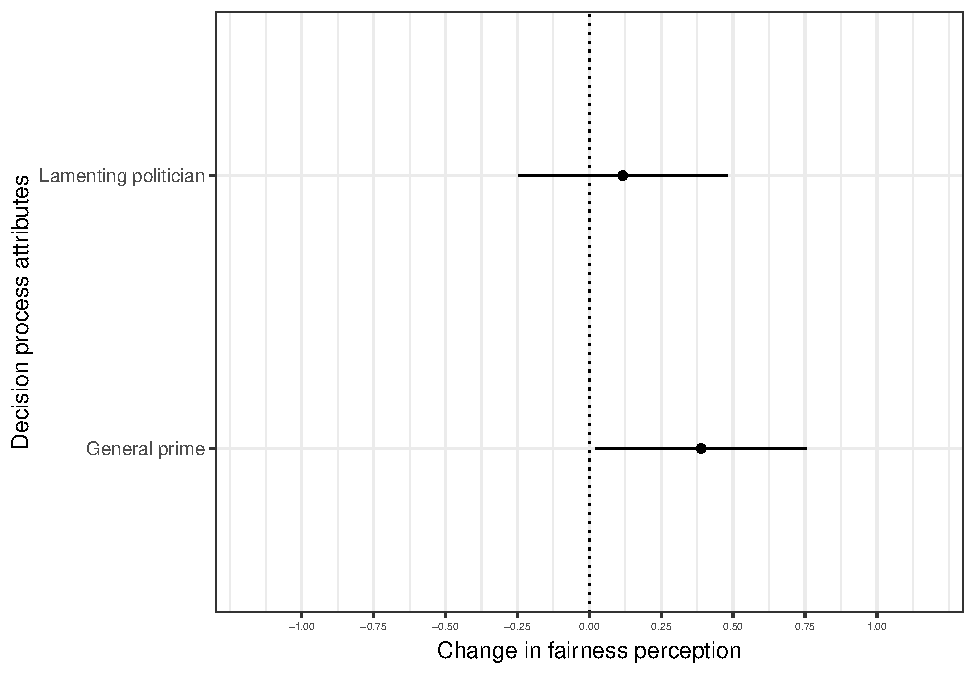
\includegraphics{Goodloser-appendix_files/figure-latex/106_post_fairness-1.pdf}

\begin{Shaded}
\begin{Highlighting}[]
\KeywordTok{ggsave}\NormalTok{(}
  \KeywordTok{here}\NormalTok{(}\StringTok{"output"}\NormalTok{, }\StringTok{"swevig"}\NormalTok{, }\StringTok{"figs"}\NormalTok{, }\StringTok{"pngs"}\NormalTok{, }\StringTok{"exp1-fairness-winners.png"}\NormalTok{),}
  \DataTypeTok{plot =}\NormalTok{ fig,}
  \DataTypeTok{width =} \FloatTok{5.5}\NormalTok{, }\DataTypeTok{height =} \FloatTok{2.75}
\NormalTok{)}

\KeywordTok{ggsave}\NormalTok{(}
  \KeywordTok{here}\NormalTok{(}\StringTok{"output"}\NormalTok{, }\StringTok{"swevig"}\NormalTok{, }\StringTok{"figs"}\NormalTok{, }\StringTok{"pdfs"}\NormalTok{, }\StringTok{"exp1-fairness-winners.pdf"}\NormalTok{),}
  \DataTypeTok{plot =}\NormalTok{ fig,}
  \DataTypeTok{width =} \FloatTok{5.5}\NormalTok{, }\DataTypeTok{height =} \FloatTok{2.75}
\NormalTok{)}


\CommentTok{#Table}
\NormalTok{table <-}\StringTok{ }\NormalTok{res_main }\OperatorTok\StringTok{ }
\StringTok{  }\KeywordTok{select}\NormalTok{(term, estimate, std.error, statistic, p.value) }\OperatorTok\StringTok{ }
\StringTok{  }\KeywordTok{mutate}\NormalTok{(}\DataTypeTok{term =} \KeywordTok{case_when}\NormalTok{( term }\OperatorTok{==}\StringTok{ "(Intercept)"} \OperatorTok{~}\StringTok{ "Not shown"}\NormalTok{,}
\NormalTok{                    term }\OperatorTok{==}\StringTok{ "treatmentLamenting politician"} \OperatorTok{~}\StringTok{ "Lamenting politician"}\NormalTok{,}
\NormalTok{                   term }\OperatorTok{==}\StringTok{ "treatmentGeneral prime"} \OperatorTok{~}\StringTok{ "General prime"}\NormalTok{)}
\NormalTok{         )}

\KeywordTok{kable}\NormalTok{(table, }\DataTypeTok{booktabs =} \OtherTok{TRUE}\NormalTok{, }\DataTypeTok{caption =} \StringTok{"Treatment effects on fairness perceptions of decision, Study 1 -- Swedish vignette"}\NormalTok{, }\DataTypeTok{col.names =} \KeywordTok{linebreak}\NormalTok{(}\KeywordTok{c}\NormalTok{(}\StringTok{"Treatment value"}\NormalTok{, }\StringTok{"Estimate"}\NormalTok{, }\StringTok{"Std. Error"}\NormalTok{, }\StringTok{"t-statistic"}\NormalTok{, }\StringTok{"p value"}\NormalTok{))) }\OperatorTok\StringTok{ }
\StringTok{  }\KeywordTok{kable_styling}\NormalTok{(}\DataTypeTok{bootstrap_options =} \KeywordTok{c}\NormalTok{(}\StringTok{"striped"}\NormalTok{, }\StringTok{"hover"}\NormalTok{, }\StringTok{"responsive"}\NormalTok{)) }
\end{Highlighting}
\end{Shaded}

(\#tab:106\_post\_fairness)Treatment effects on fairness perceptions of
decision, Study 1 -- Swedish vignette

Treatment value

Estimate

Std. Error

t-statistic

p value

Not shown

4.2849162

0.1325376

32.3298249

0.0000000

Lamenting politician

0.1160739

0.1820228

0.6376888

0.5239319

General prime

0.3886589

0.1840059

2.1122088

0.0351021

\section{Justice}\label{justice-2}

\begin{Shaded}
\begin{Highlighting}[]
\NormalTok{res_main <-}\StringTok{  }\KeywordTok{lm}\NormalTok{(justice }\OperatorTok{~}\StringTok{ }\NormalTok{treatment, }\DataTypeTok{data =}\NormalTok{ d) }
\NormalTok{res_main <-}\StringTok{ }\NormalTok{broom}\OperatorTok{::}\KeywordTok{tidy}\NormalTok{(res_main)}

\NormalTok{labels <-}\StringTok{ }\KeywordTok{data.frame}\NormalTok{(}
  \DataTypeTok{term =} \KeywordTok{c}\NormalTok{(}
    \StringTok{"treatmentLamenting politician"}\NormalTok{,}
    \StringTok{"treatmentGeneral prime"}
    
\NormalTok{  ),}
  \DataTypeTok{label =} \KeywordTok{c}\NormalTok{( }\StringTok{"Lamenting politician"}\NormalTok{,}
             \StringTok{"General prime"}\NormalTok{)}
\NormalTok{)}
\CommentTok{#Figure}
\NormalTok{fig <-}\StringTok{   }\NormalTok{res_main }\OperatorTok
\StringTok{  }\KeywordTok{filter}\NormalTok{(term }\OperatorTok{!=}\StringTok{ "(Intercept)"}\NormalTok{) }\OperatorTok\StringTok{ }
\StringTok{  }\KeywordTok{left_join}\NormalTok{(labels, }\DataTypeTok{by =} \StringTok{"term"}\NormalTok{) }\OperatorTok\StringTok{ }
\StringTok{  }
\StringTok{  }\KeywordTok{ggplot}\NormalTok{(}\KeywordTok{aes}\NormalTok{(}\DataTypeTok{x =}\NormalTok{ estimate, }\DataTypeTok{y =}\NormalTok{ label,}
             \DataTypeTok{xmin =}\NormalTok{ estimate }\OperatorTok{-}\StringTok{ }\NormalTok{(}\DecValTok{2} \OperatorTok{*}\StringTok{ }\NormalTok{std.error),}
             \DataTypeTok{xmax =}\NormalTok{ estimate }\OperatorTok{+}\StringTok{ }\NormalTok{(}\DecValTok{2} \OperatorTok{*}\StringTok{ }\NormalTok{std.error))) }\OperatorTok{+}
\StringTok{   }\KeywordTok{geom_errorbarh}\NormalTok{(}\DataTypeTok{height =} \DecValTok{0}\NormalTok{) }\OperatorTok{+}
\StringTok{  }\KeywordTok{geom_point}\NormalTok{() }\OperatorTok{+}
\StringTok{  }\KeywordTok{geom_vline}\NormalTok{(}\KeywordTok{aes}\NormalTok{(}\DataTypeTok{xintercept =} \DecValTok{0}\NormalTok{), }\DataTypeTok{linetype =} \StringTok{"dotted"}\NormalTok{) }\OperatorTok{+}
\StringTok{  }\KeywordTok{scale_x_continuous}\NormalTok{(}\DataTypeTok{limits =} \KeywordTok{c}\NormalTok{(}\OperatorTok{-}\DecValTok{1}\NormalTok{, }\DecValTok{1}\NormalTok{),}
                     \DataTypeTok{breaks =} \KeywordTok{round}\NormalTok{(}\KeywordTok{seq}\NormalTok{(}\OperatorTok{-}\DecValTok{1}\NormalTok{, }\DecValTok{1}\NormalTok{, .}\DecValTok{25}\NormalTok{), }\DecValTok{2}\NormalTok{),}
                     \DataTypeTok{expand =} \KeywordTok{c}\NormalTok{(}\DecValTok{0}\NormalTok{, }\DecValTok{0}\NormalTok{)) }\OperatorTok{+}
\StringTok{  }\KeywordTok{labs}\NormalTok{(}\DataTypeTok{x =} \StringTok{"Change in justice perception"}\NormalTok{,}
       \DataTypeTok{y =} \StringTok{"Decision process attributes"}\NormalTok{) }\OperatorTok{+}
\StringTok{  }\KeywordTok{theme_bw}\NormalTok{() }\OperatorTok{+}
\StringTok{  }\KeywordTok{theme}\NormalTok{(}\DataTypeTok{plot.margin =} \KeywordTok{unit}\NormalTok{(}\KeywordTok{c}\NormalTok{(}\DecValTok{2}\NormalTok{, }\DecValTok{2}\NormalTok{, }\DecValTok{2}\NormalTok{, }\DecValTok{2}\NormalTok{), }\StringTok{"mm"}\NormalTok{), }\DataTypeTok{axis.text.x=}\KeywordTok{element_text}\NormalTok{(}\DataTypeTok{size=}\KeywordTok{rel}\NormalTok{(}\FloatTok{0.6}\NormalTok{))) }\OperatorTok{+}
\StringTok{  }\KeywordTok{theme}\NormalTok{(}\DataTypeTok{panel.spacing =} \KeywordTok{unit}\NormalTok{(}\FloatTok{0.5}\NormalTok{, }\StringTok{"lines"}\NormalTok{))}
\NormalTok{fig}
\end{Highlighting}
\end{Shaded}

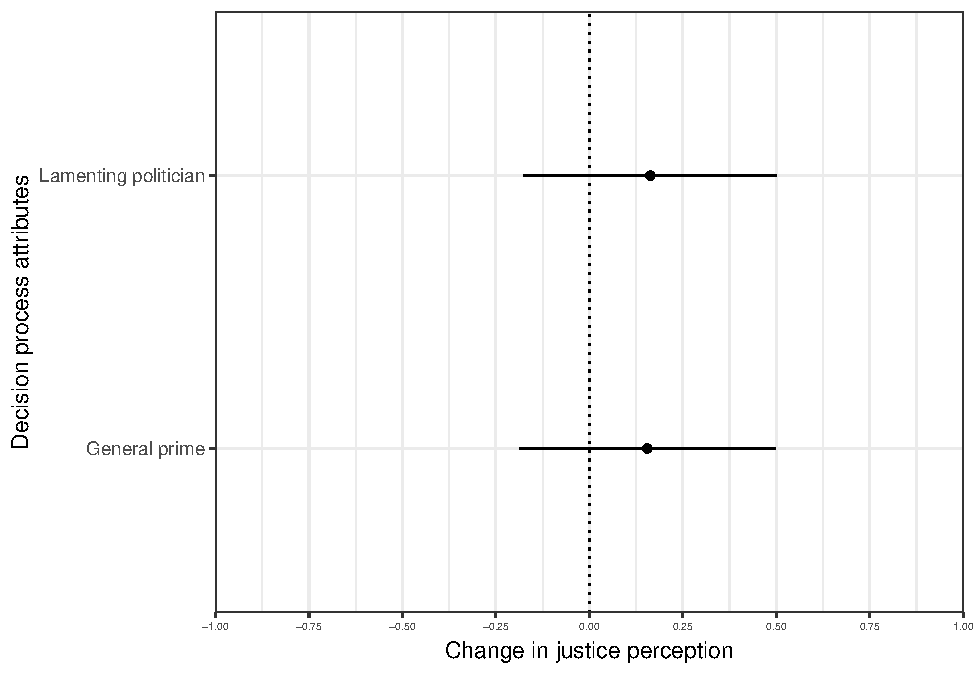
\includegraphics{Goodloser-appendix_files/figure-latex/106_post_justice-1.pdf}

\begin{Shaded}
\begin{Highlighting}[]
\KeywordTok{ggsave}\NormalTok{(}
  \KeywordTok{here}\NormalTok{(}\StringTok{"output"}\NormalTok{, }\StringTok{"swevig"}\NormalTok{, }\StringTok{"figs"}\NormalTok{, }\StringTok{"pngs"}\NormalTok{, }\StringTok{"exp1-justice-winners.png"}\NormalTok{),}
  \DataTypeTok{plot =}\NormalTok{ fig,}
  \DataTypeTok{width =} \FloatTok{5.5}\NormalTok{, }\DataTypeTok{height =} \FloatTok{2.75}
\NormalTok{)}

\KeywordTok{ggsave}\NormalTok{(}
  \KeywordTok{here}\NormalTok{(}\StringTok{"output"}\NormalTok{, }\StringTok{"swevig"}\NormalTok{, }\StringTok{"figs"}\NormalTok{, }\StringTok{"pdfs"}\NormalTok{, }\StringTok{"exp1-justice-winners.pdf"}\NormalTok{),}
  \DataTypeTok{plot =}\NormalTok{ fig,}
  \DataTypeTok{width =} \FloatTok{5.5}\NormalTok{, }\DataTypeTok{height =} \FloatTok{2.75}
\NormalTok{)}


\CommentTok{#Table}
\NormalTok{table <-}\StringTok{ }\NormalTok{res_main }\OperatorTok\StringTok{ }
\StringTok{  }\KeywordTok{select}\NormalTok{(term, estimate, std.error, statistic, p.value) }\OperatorTok\StringTok{ }
\StringTok{  }\KeywordTok{mutate}\NormalTok{(}\DataTypeTok{term =} \KeywordTok{case_when}\NormalTok{( term }\OperatorTok{==}\StringTok{ "(Intercept)"} \OperatorTok{~}\StringTok{ "Not shown"}\NormalTok{,}
\NormalTok{                    term }\OperatorTok{==}\StringTok{ "treatmentLamenting politician"} \OperatorTok{~}\StringTok{ "Lamenting politician"}\NormalTok{,}
\NormalTok{                   term }\OperatorTok{==}\StringTok{ "treatmentGeneral prime"} \OperatorTok{~}\StringTok{ "General prime"}\NormalTok{)}
\NormalTok{         )}

\KeywordTok{kable}\NormalTok{(table, }\DataTypeTok{booktabs =} \OtherTok{TRUE}\NormalTok{, }\DataTypeTok{caption =} \StringTok{"Treatment effects on justice perceptions of decision, Study 1 -- Swedish vignette"}\NormalTok{, }\DataTypeTok{col.names =} \KeywordTok{linebreak}\NormalTok{(}\KeywordTok{c}\NormalTok{(}\StringTok{"Treatment value"}\NormalTok{, }\StringTok{"Estimate"}\NormalTok{, }\StringTok{"Std. Error"}\NormalTok{, }\StringTok{"t-statistic"}\NormalTok{, }\StringTok{"p value"}\NormalTok{))) }\OperatorTok\StringTok{ }
\StringTok{  }\KeywordTok{kable_styling}\NormalTok{(}\DataTypeTok{bootstrap_options =} \KeywordTok{c}\NormalTok{(}\StringTok{"striped"}\NormalTok{, }\StringTok{"hover"}\NormalTok{, }\StringTok{"responsive"}\NormalTok{)) }
\end{Highlighting}
\end{Shaded}

(\#tab:106\_post\_justice)Treatment effects on justice perceptions of
decision, Study 1 -- Swedish vignette

Treatment value

Estimate

Std. Error

t-statistic

p value

Not shown

4.2178771

0.1231976

34.2366943

0.0000000

Lamenting politician

0.1633110

0.1691955

0.9652206

0.3348429

General prime

0.1551799

0.1710389

0.9072784

0.3646423

\section{Decision evaluation}\label{decision-evaluation-2}

\begin{Shaded}
\begin{Highlighting}[]
\NormalTok{res_main <-}\StringTok{  }\KeywordTok{lm}\NormalTok{(eval }\OperatorTok{~}\StringTok{ }\NormalTok{treatment, }\DataTypeTok{data =}\NormalTok{ d) }
\NormalTok{res_main <-}\StringTok{ }\NormalTok{broom}\OperatorTok{::}\KeywordTok{tidy}\NormalTok{(res_main)}

\NormalTok{labels <-}\StringTok{ }\KeywordTok{data.frame}\NormalTok{(}
  \DataTypeTok{term =} \KeywordTok{c}\NormalTok{(}
    \StringTok{"treatmentLamenting politician"}\NormalTok{,}
    \StringTok{"treatmentGeneral prime"}
    
\NormalTok{  ),}
  \DataTypeTok{label =} \KeywordTok{c}\NormalTok{( }\StringTok{"Lamenting politician"}\NormalTok{,}
             \StringTok{"General prime"}\NormalTok{)}
\NormalTok{)}
\CommentTok{#Figure}
\NormalTok{fig <-}\StringTok{   }\NormalTok{res_main }\OperatorTok
\StringTok{  }\KeywordTok{filter}\NormalTok{(term }\OperatorTok{!=}\StringTok{ "(Intercept)"}\NormalTok{) }\OperatorTok\StringTok{ }
\StringTok{  }\KeywordTok{left_join}\NormalTok{(labels, }\DataTypeTok{by =} \StringTok{"term"}\NormalTok{) }\OperatorTok\StringTok{ }
\StringTok{  }
\StringTok{  }\KeywordTok{ggplot}\NormalTok{(}\KeywordTok{aes}\NormalTok{(}\DataTypeTok{x =}\NormalTok{ estimate, }\DataTypeTok{y =}\NormalTok{ label,}
             \DataTypeTok{xmin =}\NormalTok{ estimate }\OperatorTok{-}\StringTok{ }\NormalTok{(}\DecValTok{2} \OperatorTok{*}\StringTok{ }\NormalTok{std.error),}
             \DataTypeTok{xmax =}\NormalTok{ estimate }\OperatorTok{+}\StringTok{ }\NormalTok{(}\DecValTok{2} \OperatorTok{*}\StringTok{ }\NormalTok{std.error))) }\OperatorTok{+}
\StringTok{   }\KeywordTok{geom_errorbarh}\NormalTok{(}\DataTypeTok{height =} \DecValTok{0}\NormalTok{) }\OperatorTok{+}
\StringTok{  }\KeywordTok{geom_point}\NormalTok{() }\OperatorTok{+}
\StringTok{  }\KeywordTok{geom_vline}\NormalTok{(}\KeywordTok{aes}\NormalTok{(}\DataTypeTok{xintercept =} \DecValTok{0}\NormalTok{), }\DataTypeTok{linetype =} \StringTok{"dotted"}\NormalTok{) }\OperatorTok{+}
\StringTok{  }\KeywordTok{scale_x_continuous}\NormalTok{(}\DataTypeTok{limits =} \KeywordTok{c}\NormalTok{(}\OperatorTok{-}\DecValTok{1}\NormalTok{, }\DecValTok{1}\NormalTok{),}
                     \DataTypeTok{breaks =} \KeywordTok{round}\NormalTok{(}\KeywordTok{seq}\NormalTok{(}\OperatorTok{-}\DecValTok{1}\NormalTok{, }\DecValTok{1}\NormalTok{, .}\DecValTok{25}\NormalTok{), }\DecValTok{2}\NormalTok{),}
                     \DataTypeTok{expand =} \KeywordTok{c}\NormalTok{(}\DecValTok{0}\NormalTok{, }\DecValTok{0}\NormalTok{)) }\OperatorTok{+}
\StringTok{  }\KeywordTok{labs}\NormalTok{(}\DataTypeTok{x =} \StringTok{"Change in decision evaluation"}\NormalTok{,}
       \DataTypeTok{y =} \StringTok{"Decision process attributes"}\NormalTok{) }\OperatorTok{+}
\StringTok{  }\KeywordTok{theme_bw}\NormalTok{() }\OperatorTok{+}
\StringTok{  }\KeywordTok{theme}\NormalTok{(}\DataTypeTok{plot.margin =} \KeywordTok{unit}\NormalTok{(}\KeywordTok{c}\NormalTok{(}\DecValTok{2}\NormalTok{, }\DecValTok{2}\NormalTok{, }\DecValTok{2}\NormalTok{, }\DecValTok{2}\NormalTok{), }\StringTok{"mm"}\NormalTok{), }\DataTypeTok{axis.text.x=}\KeywordTok{element_text}\NormalTok{(}\DataTypeTok{size=}\KeywordTok{rel}\NormalTok{(}\FloatTok{0.7}\NormalTok{))) }\OperatorTok{+}
\StringTok{  }\KeywordTok{theme}\NormalTok{(}\DataTypeTok{panel.spacing =} \KeywordTok{unit}\NormalTok{(}\FloatTok{0.5}\NormalTok{, }\StringTok{"lines"}\NormalTok{))}
\NormalTok{fig}
\end{Highlighting}
\end{Shaded}

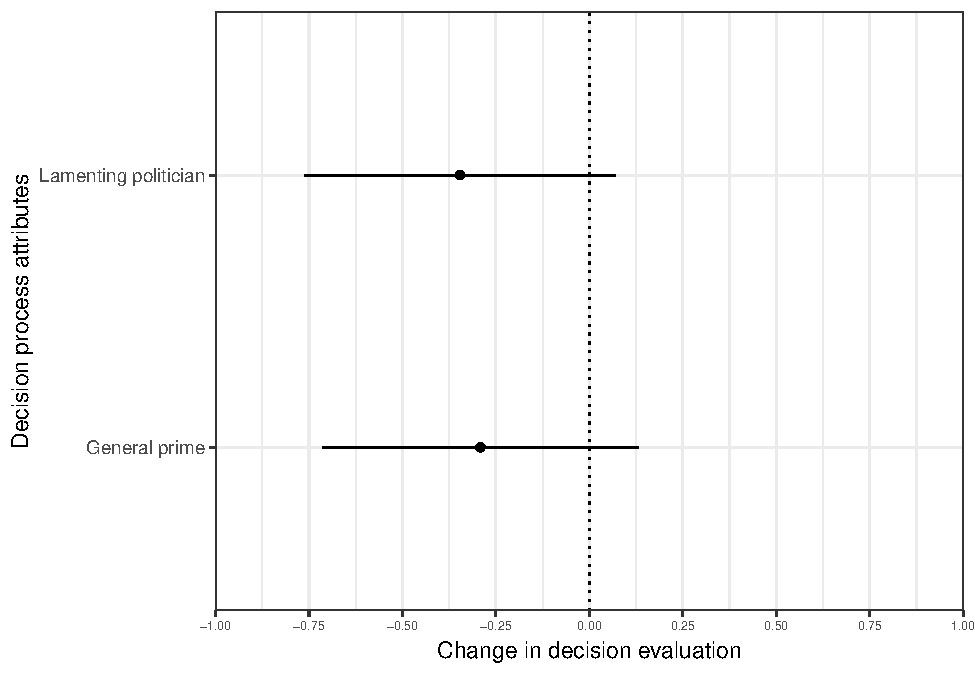
\includegraphics{Goodloser-appendix_files/figure-latex/106_post_eval-1.pdf}

\begin{Shaded}
\begin{Highlighting}[]
\KeywordTok{ggsave}\NormalTok{(}
  \KeywordTok{here}\NormalTok{(}\StringTok{"output"}\NormalTok{, }\StringTok{"swevig"}\NormalTok{, }\StringTok{"figs"}\NormalTok{, }\StringTok{"pngs"}\NormalTok{, }\StringTok{"exp1-eval-winners.png"}\NormalTok{),}
  \DataTypeTok{plot =}\NormalTok{ fig,}
  \DataTypeTok{width =} \FloatTok{5.5}\NormalTok{, }\DataTypeTok{height =} \FloatTok{2.75}
\NormalTok{)}

\KeywordTok{ggsave}\NormalTok{(}
  \KeywordTok{here}\NormalTok{(}\StringTok{"output"}\NormalTok{, }\StringTok{"swevig"}\NormalTok{, }\StringTok{"figs"}\NormalTok{, }\StringTok{"pdfs"}\NormalTok{, }\StringTok{"exp1-eval-winners.pdf"}\NormalTok{),}
  \DataTypeTok{plot =}\NormalTok{ fig,}
  \DataTypeTok{width =} \FloatTok{5.5}\NormalTok{, }\DataTypeTok{height =} \FloatTok{2.75}
\NormalTok{)}


\CommentTok{#Table}
\NormalTok{table <-}\StringTok{ }\NormalTok{res_main }\OperatorTok\StringTok{ }
\StringTok{  }\KeywordTok{select}\NormalTok{(term, estimate, std.error, statistic, p.value) }\OperatorTok\StringTok{ }
\StringTok{  }\KeywordTok{mutate}\NormalTok{(}\DataTypeTok{term =} \KeywordTok{case_when}\NormalTok{( term }\OperatorTok{==}\StringTok{ "(Intercept)"} \OperatorTok{~}\StringTok{ "Not shown"}\NormalTok{,}
\NormalTok{                    term }\OperatorTok{==}\StringTok{ "treatmentLamenting politician"} \OperatorTok{~}\StringTok{ "Lamenting politician"}\NormalTok{,}
\NormalTok{                   term }\OperatorTok{==}\StringTok{ "treatmentGeneral prime"} \OperatorTok{~}\StringTok{ "General prime"}\NormalTok{)}
\NormalTok{         )}

\KeywordTok{kable}\NormalTok{(table, }\DataTypeTok{booktabs =} \OtherTok{TRUE}\NormalTok{, }\DataTypeTok{caption =} \StringTok{"Treatment effects on decision evaluation, Study 1 -- Swedish vignette"}\NormalTok{, }\DataTypeTok{col.names =} \KeywordTok{linebreak}\NormalTok{(}\KeywordTok{c}\NormalTok{(}\StringTok{"Treatment value"}\NormalTok{, }\StringTok{"Estimate"}\NormalTok{, }\StringTok{"Std. Error"}\NormalTok{, }\StringTok{"t-statistic"}\NormalTok{, }\StringTok{"p value"}\NormalTok{))) }\OperatorTok\StringTok{ }
\StringTok{  }\KeywordTok{kable_styling}\NormalTok{(}\DataTypeTok{bootstrap_options =} \KeywordTok{c}\NormalTok{(}\StringTok{"striped"}\NormalTok{, }\StringTok{"hover"}\NormalTok{, }\StringTok{"responsive"}\NormalTok{)) }
\end{Highlighting}
\end{Shaded}

(\#tab:106\_post\_eval)Treatment effects on decision evaluation, Study 1
-- Swedish vignette

Treatment value

Estimate

Std. Error

t-statistic

p value

Not shown

4.5139665

0.1517737

29.741418

0.0000000

Lamenting politician

-0.3456496

0.2084412

-1.658260

0.0978142

General prime

-0.2911686

0.2107121

-1.381831

0.1675639

\section{Willingness to accept}\label{willingness-to-accept-2}

\begin{Shaded}
\begin{Highlighting}[]
\NormalTok{res_main <-}\StringTok{  }\KeywordTok{lm}\NormalTok{(accept }\OperatorTok{~}\StringTok{ }\NormalTok{treatment, }\DataTypeTok{data =}\NormalTok{ d) }
\NormalTok{res_main <-}\StringTok{ }\NormalTok{broom}\OperatorTok{::}\KeywordTok{tidy}\NormalTok{(res_main)}

\NormalTok{labels <-}\StringTok{ }\KeywordTok{data.frame}\NormalTok{(}
  \DataTypeTok{term =} \KeywordTok{c}\NormalTok{(}
    \StringTok{"treatmentLamenting politician"}\NormalTok{,}
    \StringTok{"treatmentGeneral prime"}
    
\NormalTok{  ),}
  \DataTypeTok{label =} \KeywordTok{c}\NormalTok{( }\StringTok{"Lamenting politician"}\NormalTok{,}
             \StringTok{"General prime"}\NormalTok{)}
\NormalTok{)}
\CommentTok{#Figure}
\NormalTok{fig <-}\StringTok{   }\NormalTok{res_main }\OperatorTok
\StringTok{  }\KeywordTok{filter}\NormalTok{(term }\OperatorTok{!=}\StringTok{ "(Intercept)"}\NormalTok{) }\OperatorTok\StringTok{ }
\StringTok{  }\KeywordTok{left_join}\NormalTok{(labels, }\DataTypeTok{by =} \StringTok{"term"}\NormalTok{) }\OperatorTok\StringTok{ }
\StringTok{  }
\StringTok{  }\KeywordTok{ggplot}\NormalTok{(}\KeywordTok{aes}\NormalTok{(}\DataTypeTok{x =}\NormalTok{ estimate, }\DataTypeTok{y =}\NormalTok{ label,}
             \DataTypeTok{xmin =}\NormalTok{ estimate }\OperatorTok{-}\StringTok{ }\NormalTok{(}\DecValTok{2} \OperatorTok{*}\StringTok{ }\NormalTok{std.error),}
             \DataTypeTok{xmax =}\NormalTok{ estimate }\OperatorTok{+}\StringTok{ }\NormalTok{(}\DecValTok{2} \OperatorTok{*}\StringTok{ }\NormalTok{std.error))) }\OperatorTok{+}
\StringTok{   }\KeywordTok{geom_errorbarh}\NormalTok{(}\DataTypeTok{height =} \DecValTok{0}\NormalTok{) }\OperatorTok{+}
\StringTok{  }\KeywordTok{geom_point}\NormalTok{() }\OperatorTok{+}
\StringTok{  }\KeywordTok{geom_vline}\NormalTok{(}\KeywordTok{aes}\NormalTok{(}\DataTypeTok{xintercept =} \DecValTok{0}\NormalTok{), }\DataTypeTok{linetype =} \StringTok{"dotted"}\NormalTok{) }\OperatorTok{+}
\StringTok{  }\KeywordTok{scale_x_continuous}\NormalTok{(}\DataTypeTok{limits =} \KeywordTok{c}\NormalTok{(}\OperatorTok{-}\DecValTok{1}\NormalTok{, }\DecValTok{1}\NormalTok{),}
                     \DataTypeTok{breaks =} \KeywordTok{round}\NormalTok{(}\KeywordTok{seq}\NormalTok{(}\OperatorTok{-}\DecValTok{1}\NormalTok{, }\DecValTok{1}\NormalTok{, .}\DecValTok{25}\NormalTok{), }\DecValTok{2}\NormalTok{),}
                     \DataTypeTok{expand =} \KeywordTok{c}\NormalTok{(}\DecValTok{0}\NormalTok{, }\DecValTok{0}\NormalTok{)) }\OperatorTok{+}
\StringTok{  }\KeywordTok{labs}\NormalTok{(}\DataTypeTok{x =} \StringTok{"Change in willingness to accept outcome"}\NormalTok{,}
       \DataTypeTok{y =} \StringTok{"Decision process attributes"}\NormalTok{) }\OperatorTok{+}
\StringTok{  }\KeywordTok{theme_bw}\NormalTok{() }\OperatorTok{+}
\StringTok{  }\KeywordTok{theme}\NormalTok{(}\DataTypeTok{plot.margin =} \KeywordTok{unit}\NormalTok{(}\KeywordTok{c}\NormalTok{(}\DecValTok{2}\NormalTok{, }\DecValTok{2}\NormalTok{, }\DecValTok{2}\NormalTok{, }\DecValTok{2}\NormalTok{), }\StringTok{"mm"}\NormalTok{), }\DataTypeTok{axis.text.x=}\KeywordTok{element_text}\NormalTok{(}\DataTypeTok{size=}\KeywordTok{rel}\NormalTok{(}\FloatTok{0.6}\NormalTok{))) }\OperatorTok{+}
\StringTok{  }\KeywordTok{theme}\NormalTok{(}\DataTypeTok{panel.spacing =} \KeywordTok{unit}\NormalTok{(}\FloatTok{0.5}\NormalTok{, }\StringTok{"lines"}\NormalTok{))}
\NormalTok{fig}
\end{Highlighting}
\end{Shaded}

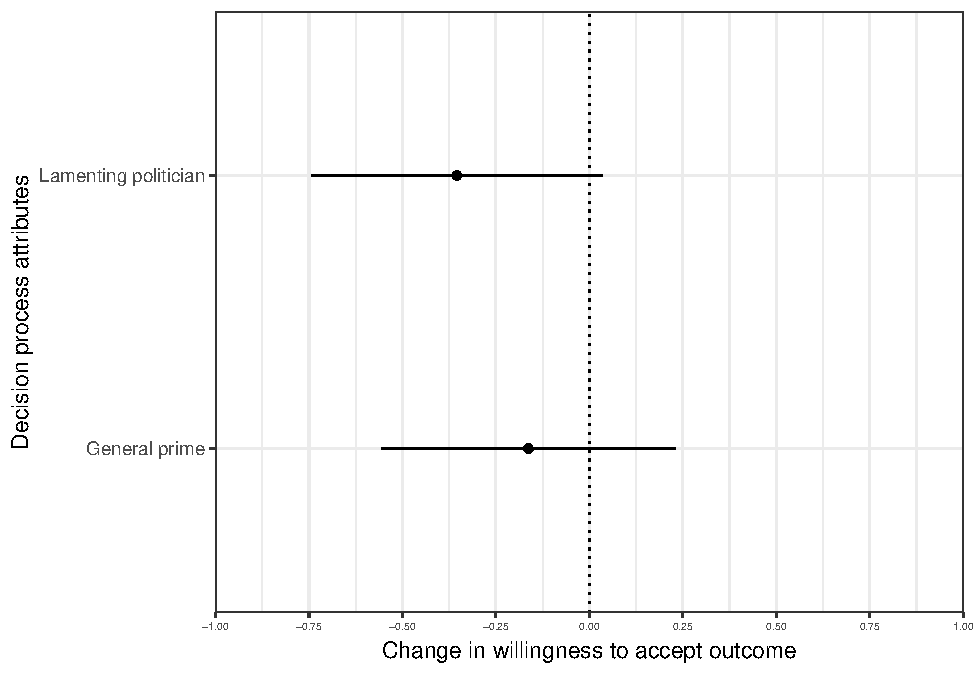
\includegraphics{Goodloser-appendix_files/figure-latex/106_post_accept-1.pdf}

\begin{Shaded}
\begin{Highlighting}[]
\KeywordTok{ggsave}\NormalTok{(}
  \KeywordTok{here}\NormalTok{(}\StringTok{"output"}\NormalTok{, }\StringTok{"swevig"}\NormalTok{, }\StringTok{"figs"}\NormalTok{, }\StringTok{"pngs"}\NormalTok{, }\StringTok{"exp1-accept-winners.png"}\NormalTok{),}
  \DataTypeTok{plot =}\NormalTok{ fig,}
  \DataTypeTok{width =} \FloatTok{5.5}\NormalTok{, }\DataTypeTok{height =} \FloatTok{2.75}
\NormalTok{)}

\KeywordTok{ggsave}\NormalTok{(}
  \KeywordTok{here}\NormalTok{(}\StringTok{"output"}\NormalTok{, }\StringTok{"swevig"}\NormalTok{, }\StringTok{"figs"}\NormalTok{, }\StringTok{"pdfs"}\NormalTok{, }\StringTok{"exp1-accept-winners.pdf"}\NormalTok{),}
  \DataTypeTok{plot =}\NormalTok{ fig,}
  \DataTypeTok{width =} \FloatTok{5.5}\NormalTok{, }\DataTypeTok{height =} \FloatTok{2.75}
\NormalTok{)}


\CommentTok{#Table}
\NormalTok{table <-}\StringTok{ }\NormalTok{res_main }\OperatorTok\StringTok{ }
\StringTok{  }\KeywordTok{select}\NormalTok{(term, estimate, std.error, statistic, p.value) }\OperatorTok\StringTok{ }
\StringTok{  }\KeywordTok{mutate}\NormalTok{(}\DataTypeTok{term =} \KeywordTok{case_when}\NormalTok{( term }\OperatorTok{==}\StringTok{ "(Intercept)"} \OperatorTok{~}\StringTok{ "Not shown"}\NormalTok{,}
\NormalTok{                    term }\OperatorTok{==}\StringTok{ "treatmentLamenting politician"} \OperatorTok{~}\StringTok{ "Lamenting politician"}\NormalTok{,}
\NormalTok{                   term }\OperatorTok{==}\StringTok{ "treatmentGeneral prime"} \OperatorTok{~}\StringTok{ "General prime"}\NormalTok{)}
\NormalTok{         )}

\KeywordTok{kable}\NormalTok{(table, }\DataTypeTok{booktabs =} \OtherTok{TRUE}\NormalTok{, }\DataTypeTok{caption =} \StringTok{"Treatment effects on willingness to accept decision, Study 1 -- Swedish vignette"}\NormalTok{, }\DataTypeTok{col.names =} \KeywordTok{linebreak}\NormalTok{(}\KeywordTok{c}\NormalTok{(}\StringTok{"Treatment value"}\NormalTok{, }\StringTok{"Estimate"}\NormalTok{, }\StringTok{"Std. Error"}\NormalTok{, }\StringTok{"t-statistic"}\NormalTok{, }\StringTok{"p value"}\NormalTok{))) }\OperatorTok\StringTok{ }
\StringTok{  }\KeywordTok{kable_styling}\NormalTok{(}\DataTypeTok{bootstrap_options =} \KeywordTok{c}\NormalTok{(}\StringTok{"striped"}\NormalTok{, }\StringTok{"hover"}\NormalTok{, }\StringTok{"responsive"}\NormalTok{)) }
\end{Highlighting}
\end{Shaded}

(\#tab:106\_post\_accept)Treatment effects on willingness to accept
decision, Study 1 -- Swedish vignette

Treatment value

Estimate

Std. Error

t-statistic

p value

Not shown

5.4581006

0.1414642

38.5829139

0.0000000

Lamenting politician

-0.3541402

0.1942823

-1.8228120

0.0688547

General prime

-0.1627638

0.1963990

-0.8287402

0.4075977

\section{Compliance}\label{compliance-2}

\begin{Shaded}
\begin{Highlighting}[]
\NormalTok{res_main <-}\StringTok{  }\KeywordTok{lm}\NormalTok{(comply }\OperatorTok{~}\StringTok{ }\NormalTok{treatment, }\DataTypeTok{data =}\NormalTok{ d) }
\NormalTok{res_main <-}\StringTok{ }\NormalTok{broom}\OperatorTok{::}\KeywordTok{tidy}\NormalTok{(res_main)}

\NormalTok{labels <-}\StringTok{ }\KeywordTok{data.frame}\NormalTok{(}
  \DataTypeTok{term =} \KeywordTok{c}\NormalTok{(}
    \StringTok{"treatmentLamenting politician"}\NormalTok{,}
    \StringTok{"treatmentGeneral prime"}
    
\NormalTok{  ),}
  \DataTypeTok{label =} \KeywordTok{c}\NormalTok{( }\StringTok{"Lamenting politician"}\NormalTok{,}
             \StringTok{"General prime"}\NormalTok{)}
\NormalTok{)}
\CommentTok{#Figure}
\NormalTok{fig <-}\StringTok{   }\NormalTok{res_main }\OperatorTok
\StringTok{  }\KeywordTok{filter}\NormalTok{(term }\OperatorTok{!=}\StringTok{ "(Intercept)"}\NormalTok{) }\OperatorTok\StringTok{ }
\StringTok{  }\KeywordTok{left_join}\NormalTok{(labels, }\DataTypeTok{by =} \StringTok{"term"}\NormalTok{) }\OperatorTok\StringTok{ }
\StringTok{  }
\StringTok{  }\KeywordTok{ggplot}\NormalTok{(}\KeywordTok{aes}\NormalTok{(}\DataTypeTok{x =}\NormalTok{ estimate, }\DataTypeTok{y =}\NormalTok{ label,}
             \DataTypeTok{xmin =}\NormalTok{ estimate }\OperatorTok{-}\StringTok{ }\NormalTok{(}\DecValTok{2} \OperatorTok{*}\StringTok{ }\NormalTok{std.error),}
             \DataTypeTok{xmax =}\NormalTok{ estimate }\OperatorTok{+}\StringTok{ }\NormalTok{(}\DecValTok{2} \OperatorTok{*}\StringTok{ }\NormalTok{std.error))) }\OperatorTok{+}
\StringTok{   }\KeywordTok{geom_errorbarh}\NormalTok{(}\DataTypeTok{height =} \DecValTok{0}\NormalTok{) }\OperatorTok{+}
\StringTok{  }\KeywordTok{geom_point}\NormalTok{() }\OperatorTok{+}
\StringTok{  }\KeywordTok{geom_vline}\NormalTok{(}\KeywordTok{aes}\NormalTok{(}\DataTypeTok{xintercept =} \DecValTok{0}\NormalTok{), }\DataTypeTok{linetype =} \StringTok{"dotted"}\NormalTok{) }\OperatorTok{+}
\StringTok{  }\KeywordTok{scale_x_continuous}\NormalTok{(}\DataTypeTok{limits =} \KeywordTok{c}\NormalTok{(}\OperatorTok{-}\DecValTok{1}\NormalTok{, }\DecValTok{1}\NormalTok{),}
                     \DataTypeTok{breaks =} \KeywordTok{round}\NormalTok{(}\KeywordTok{seq}\NormalTok{(}\OperatorTok{-}\DecValTok{1}\NormalTok{, }\DecValTok{1}\NormalTok{, .}\DecValTok{25}\NormalTok{), }\DecValTok{2}\NormalTok{),}
                     \DataTypeTok{expand =} \KeywordTok{c}\NormalTok{(}\DecValTok{0}\NormalTok{, }\DecValTok{0}\NormalTok{)) }\OperatorTok{+}
\StringTok{  }\KeywordTok{labs}\NormalTok{(}\DataTypeTok{x =} \StringTok{"Change in decision compliance"}\NormalTok{,}
       \DataTypeTok{y =} \StringTok{"Decision process attributes"}\NormalTok{) }\OperatorTok{+}
\StringTok{  }\KeywordTok{theme_bw}\NormalTok{() }\OperatorTok{+}
\StringTok{  }\KeywordTok{theme}\NormalTok{(}\DataTypeTok{plot.margin =} \KeywordTok{unit}\NormalTok{(}\KeywordTok{c}\NormalTok{(}\DecValTok{2}\NormalTok{, }\DecValTok{2}\NormalTok{, }\DecValTok{2}\NormalTok{, }\DecValTok{2}\NormalTok{), }\StringTok{"mm"}\NormalTok{), }\DataTypeTok{axis.text.x=}\KeywordTok{element_text}\NormalTok{(}\DataTypeTok{size=}\KeywordTok{rel}\NormalTok{(}\FloatTok{0.6}\NormalTok{))) }\OperatorTok{+}
\StringTok{  }\KeywordTok{theme}\NormalTok{(}\DataTypeTok{panel.spacing =} \KeywordTok{unit}\NormalTok{(}\FloatTok{0.5}\NormalTok{, }\StringTok{"lines"}\NormalTok{))}
\NormalTok{fig}
\end{Highlighting}
\end{Shaded}

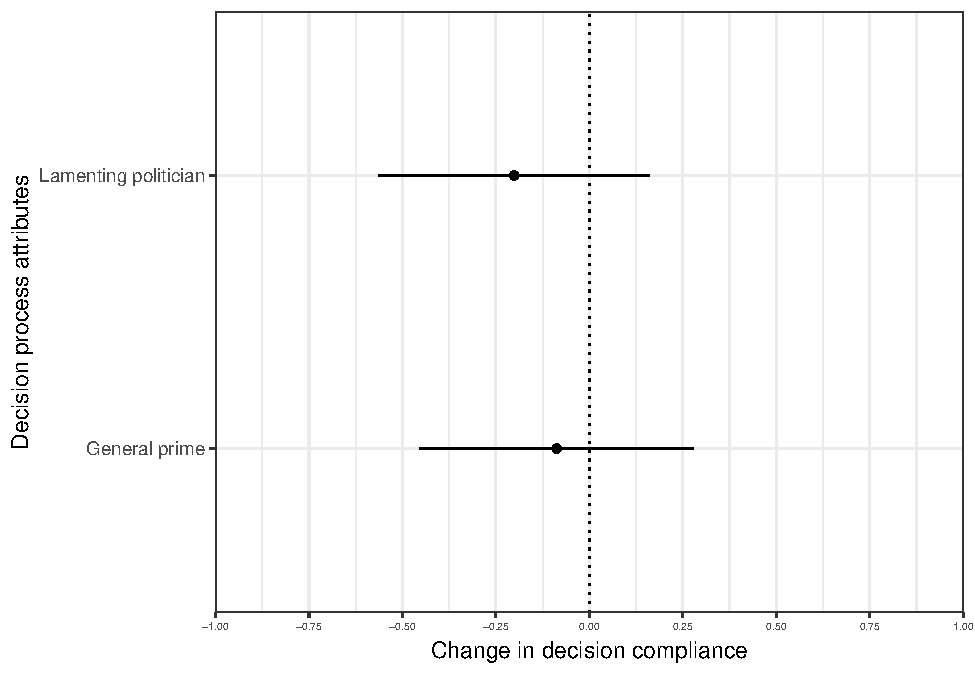
\includegraphics{Goodloser-appendix_files/figure-latex/106_post_comply-1.pdf}

\begin{Shaded}
\begin{Highlighting}[]
\KeywordTok{ggsave}\NormalTok{(}
  \KeywordTok{here}\NormalTok{(}\StringTok{"output"}\NormalTok{, }\StringTok{"swevig"}\NormalTok{, }\StringTok{"figs"}\NormalTok{, }\StringTok{"pngs"}\NormalTok{, }\StringTok{"exp1-comply-winners.png"}\NormalTok{),}
  \DataTypeTok{plot =}\NormalTok{ fig,}
  \DataTypeTok{width =} \FloatTok{5.5}\NormalTok{, }\DataTypeTok{height =} \FloatTok{2.75}
\NormalTok{)}

\KeywordTok{ggsave}\NormalTok{(}
  \KeywordTok{here}\NormalTok{(}\StringTok{"output"}\NormalTok{, }\StringTok{"swevig"}\NormalTok{, }\StringTok{"figs"}\NormalTok{, }\StringTok{"pdfs"}\NormalTok{, }\StringTok{"exp1-comply-winners.pdf"}\NormalTok{),}
  \DataTypeTok{plot =}\NormalTok{ fig,}
  \DataTypeTok{width =} \FloatTok{5.5}\NormalTok{, }\DataTypeTok{height =} \FloatTok{2.75}
\NormalTok{)}


\CommentTok{#Table}
\NormalTok{table <-}\StringTok{ }\NormalTok{res_main }\OperatorTok\StringTok{ }
\StringTok{  }\KeywordTok{select}\NormalTok{(term, estimate, std.error, statistic, p.value) }\OperatorTok\StringTok{ }
\StringTok{  }\KeywordTok{mutate}\NormalTok{(}\DataTypeTok{term =} \KeywordTok{case_when}\NormalTok{( term }\OperatorTok{==}\StringTok{ "(Intercept)"} \OperatorTok{~}\StringTok{ "Not shown"}\NormalTok{,}
\NormalTok{                    term }\OperatorTok{==}\StringTok{ "treatmentLamenting politician"} \OperatorTok{~}\StringTok{ "Lamenting politician"}\NormalTok{,}
\NormalTok{                   term }\OperatorTok{==}\StringTok{ "treatmentGeneral prime"} \OperatorTok{~}\StringTok{ "General prime"}\NormalTok{)}
\NormalTok{         )}

\KeywordTok{kable}\NormalTok{(table, }\DataTypeTok{booktabs =} \OtherTok{TRUE}\NormalTok{, }\DataTypeTok{caption =} \StringTok{"Treatment effects on decision compliance, Study 1 -- Swedish vignette"}\NormalTok{, }\DataTypeTok{col.names =} \KeywordTok{linebreak}\NormalTok{(}\KeywordTok{c}\NormalTok{(}\StringTok{"Treatment value"}\NormalTok{, }\StringTok{"Estimate"}\NormalTok{, }\StringTok{"Std. Error"}\NormalTok{, }\StringTok{"t-statistic"}\NormalTok{, }\StringTok{"p value"}\NormalTok{))) }\OperatorTok\StringTok{ }
\StringTok{  }\KeywordTok{kable_styling}\NormalTok{(}\DataTypeTok{bootstrap_options =} \KeywordTok{c}\NormalTok{(}\StringTok{"striped"}\NormalTok{, }\StringTok{"hover"}\NormalTok{, }\StringTok{"responsive"}\NormalTok{)) }
\end{Highlighting}
\end{Shaded}

(\#tab:106\_post\_comply)Treatment effects on decision compliance, Study
1 -- Swedish vignette

Treatment value

Estimate

Std. Error

t-statistic

p value

Not shown

5.4189944

0.1317730

41.1237227

0.0000000

Lamenting politician

-0.2011726

0.1809727

-1.1116186

0.2667700

General prime

-0.0873882

0.1829444

-0.4776763

0.6330634

\part{STUDY II: NORWEGIAN
VIGNETTE}\label{part-study-ii-norwegian-vignette}

The experiment was fielded in Norway during the spring and fall of 2017
during the 9th and 10th waves of
\href{https://www.uib.no/medborger}{Norwegian Citizen Panel (NCP)}. The
NCP is a research-purpose internet panel with over 6000 active
participants. It is based on a probability sample of the general
Norwegian population above the age of 18 drawn from the Norwegian
National Registry. The survey is based on a online questionnaire with
postal recruitment. Panel members complete a questionnaire three times a
year of 15 minutes each. The NCP is a core component of The Digital
Social Science Core Facilities (DIGSSCORE), and was established in 2013
as a collaboration between several departments at the Faculty of Social
Sciences at the University of Bergen and NORCE -- Norwegian Research
Centre. We refer to the
\href{Data/ncp-wave13-documentation.pdf}{documentation report} for
further details on technical aspects of the survey, panel recruitment,
response rates of the 13th wave, and representativeness. For details
about the data collected in this project and the NCP at large, we refer
to the \href{Data/ncp-wave13-codebook.pdf}{codebook for the Waves 1-13}.

\chapter{Create Data Set}\label{create-data-set-1}

\begin{quote}
This chapter describes the process of loading the full NCP data set and
from that creating a sample data set with the relevant variables for the
Good Loser conjoint experiment.
\end{quote}

\section{Load packages or install them if not already
installed}\label{load-packages-or-install-them-if-not-already-installed-1}

\begin{Shaded}
\begin{Highlighting}[]
\ControlFlowTok{if}\NormalTok{(}\OperatorTok{!}\KeywordTok{require}\NormalTok{(}\StringTok{"ggplot2"}\NormalTok{))\{}\KeywordTok{install.packages}\NormalTok{(}\StringTok{"ggplot2"}\NormalTok{);  }\KeywordTok{library}\NormalTok{(ggplot2)\}}
\ControlFlowTok{if}\NormalTok{(}\OperatorTok{!}\KeywordTok{require}\NormalTok{(}\StringTok{"ggthemes"}\NormalTok{))\{}\KeywordTok{install.packages}\NormalTok{(}\StringTok{"ggthemes"}\NormalTok{);  }\KeywordTok{library}\NormalTok{(ggthemes)\}}
\ControlFlowTok{if}\NormalTok{(}\OperatorTok{!}\KeywordTok{require}\NormalTok{(}\StringTok{"haven"}\NormalTok{))\{}\KeywordTok{install.packages}\NormalTok{(}\StringTok{"haven"}\NormalTok{);  }\KeywordTok{library}\NormalTok{(haven)\}}
\ControlFlowTok{if}\NormalTok{(}\OperatorTok{!}\KeywordTok{require}\NormalTok{(}\StringTok{"Hmisc"}\NormalTok{))\{}\KeywordTok{install.packages}\NormalTok{(}\StringTok{"Hmisc"}\NormalTok{);  }\KeywordTok{library}\NormalTok{(Hmisc)\}}
\ControlFlowTok{if}\NormalTok{(}\OperatorTok{!}\KeywordTok{require}\NormalTok{(}\StringTok{"knitr"}\NormalTok{))\{}\KeywordTok{install.packages}\NormalTok{(}\StringTok{"knitr"}\NormalTok{);  }\KeywordTok{library}\NormalTok{(knitr)\}}
\ControlFlowTok{if}\NormalTok{(}\OperatorTok{!}\KeywordTok{require}\NormalTok{(}\StringTok{"likert"}\NormalTok{))\{}\KeywordTok{install.packages}\NormalTok{(}\StringTok{"likert"}\NormalTok{);  }\KeywordTok{library}\NormalTok{(likert)\}}
\ControlFlowTok{if}\NormalTok{(}\OperatorTok{!}\KeywordTok{require}\NormalTok{(}\StringTok{"naniar"}\NormalTok{))\{}\KeywordTok{install.packages}\NormalTok{(}\StringTok{"naniar"}\NormalTok{);  }\KeywordTok{library}\NormalTok{(naniar)\}}
\ControlFlowTok{if}\NormalTok{(}\OperatorTok{!}\KeywordTok{require}\NormalTok{(}\StringTok{"readxl"}\NormalTok{))\{}\KeywordTok{install.packages}\NormalTok{(}\StringTok{"readxl"}\NormalTok{);  }\KeywordTok{library}\NormalTok{(readxl)\}}
\ControlFlowTok{if}\NormalTok{(}\OperatorTok{!}\KeywordTok{require}\NormalTok{(}\StringTok{"tidyverse"}\NormalTok{))\{}\KeywordTok{install.packages}\NormalTok{(}\StringTok{"tidyverse"}\NormalTok{);  }\KeywordTok{library}\NormalTok{(tidyverse)\}}

\NormalTok{## Utils.}
\KeywordTok{source}\NormalTok{(}\StringTok{"goodloser-utils.R"}\NormalTok{)}

\NormalTok{knitr}\OperatorTok{::}\NormalTok{opts_chunk}\OperatorTok{$}\KeywordTok{set}\NormalTok{(}\DataTypeTok{echo =} \OtherTok{FALSE}\NormalTok{, }\DataTypeTok{knitr.kable.NA =} \StringTok{""}\NormalTok{, }\DataTypeTok{cache =} \OtherTok{FALSE}\NormalTok{, }\DataTypeTok{warning =} \OtherTok{FALSE}\NormalTok{, }\DataTypeTok{message =} \OtherTok{FALSE}\NormalTok{, }\DataTypeTok{error =} \OtherTok{TRUE}\NormalTok{, }\DataTypeTok{echo =} \OtherTok{FALSE}\NormalTok{)}
\end{Highlighting}
\end{Shaded}

\section{Load raw NCP data}\label{load-raw-ncp-data}

Select variables of interest, and create new data set in .sav and .csv
formats

\begin{Shaded}
\begin{Highlighting}[]
\NormalTok{ncp_raw <-}\StringTok{ }\KeywordTok{read_sav}\NormalTok{(}\StringTok{"C:}\CharTok{\textbackslash{}\textbackslash{}}\StringTok{Users/Sveinung/OneDrive/NORCE 2018-/goodloser/Conjoint/Bookdown-goodloser/Data/Norwegian Citizen Panel - wave 1-13 - EN.sav"}\NormalTok{) }

\NormalTok{d  <-}\StringTok{ }\NormalTok{ncp_raw }\OperatorTok\StringTok{ }
\StringTok{                     }\KeywordTok{select}\NormalTok{(}
\NormalTok{                       responseid,}
\NormalTok{                       r9pad1, }
\NormalTok{                       r9pad2, }
\NormalTok{                       r9pad3, }
\NormalTok{                       r10panelpad, }
\NormalTok{                       r10pad1, }
\NormalTok{                       r10pad2, }
\NormalTok{                       r10pad3_mobil, }
\NormalTok{                       r10pad3a_ran, }
\NormalTok{                       r10pad3b_ran, }
\NormalTok{                       r10pad3ended, }
\NormalTok{                       r10pad3error, }
\NormalTok{                       r10pad3paused,}
\NormalTok{                       r10pad3played,}
\NormalTok{                       r10pad3_timespent, }
\NormalTok{                       r10pad4, }
\NormalTok{                       r10pad4_comment,}
\NormalTok{                       r10pad5, }
\NormalTok{                       r10pad6, }
\NormalTok{                       r10pad7, }
\NormalTok{                       r10pad8, }
\NormalTok{                       r10pad9, }
\NormalTok{                       r10pad1_9_backward_}\DecValTok{1}\NormalTok{, }
\NormalTok{                       r10pad1_9_backward_}\DecValTok{2}\NormalTok{, }
\NormalTok{                       r10pad1_9_backward_}\DecValTok{3}\NormalTok{, }
\NormalTok{                       r10pad1_9_backward_}\DecValTok{4}\NormalTok{, }
\NormalTok{                       r10pad1_9_backward_}\DecValTok{5}\NormalTok{, }
\NormalTok{                       r10pad1_9_backward_}\DecValTok{6}\NormalTok{, }
\NormalTok{                       r10pad1_9_backward_}\DecValTok{7}\NormalTok{, }
\NormalTok{                       r10pad1_9_backward_}\DecValTok{8} 
\NormalTok{                     ) }

\CommentTok{#Create data file, .csv format}
  \KeywordTok{write.csv}\NormalTok{(d, }\StringTok{"Data/Goodloser-exp2.csv"}\NormalTok{) }
  \CommentTok{#Create data file, .sav format}
  \KeywordTok{write_sav}\NormalTok{(d, }\StringTok{"Data/Goodloser-exp2.sav"}\NormalTok{, }\DataTypeTok{compress =} \OtherTok{FALSE}\NormalTok{) }
\end{Highlighting}
\end{Shaded}

\chapter{Codebook}\label{codebook-1}

\begin{quote}
This chapter displays the codebook for the data set of the first Good
Loser experiment, generated using the R package ``codebook''.
\end{quote}

\begin{verbatim}
## # A tibble: 17,011 x 30
##    responseid r9pad1 r9pad2 r9pad3 r10panelpad r10pad1 r10pad2
##         <dbl> <dbl+> <dbl+> <dbl+> <dbl+lbl>   <dbl+l> <dbl+l>
##  1         NA NA     NA     NA     NA          NA      NA     
##  2    1000001 NA     NA     NA      0          98      98     
##  3    1000002 NA     NA     NA      0          98      98     
##  4    1000003 NA     NA     NA     NA          NA      NA     
##  5    1000004 NA     NA     NA     NA          NA      NA     
##  6    1000005 NA     NA     NA     NA          NA      NA     
##  7    1000006 NA     NA     NA     NA          NA      NA     
##  8    1000007 98     98     98     NA          NA      NA     
##  9    1000008 NA     NA     NA     NA          NA      NA     
## 10    1000009 NA     NA     NA     NA          NA      NA     
## # ... with 17,001 more rows, and 23 more variables:
## #   r10pad3_mobil <dbl+lbl>, r10pad3a_ran <dbl+lbl>,
## #   r10pad3b_ran <dbl+lbl>, r10pad3ended <dbl>, r10pad3error <dbl>,
## #   r10pad3paused <dbl>, r10pad3played <dbl>, r10pad3_timespent <dbl>,
## #   r10pad4 <dbl+lbl>, r10pad4_comment <chr>, r10pad5 <dbl+lbl>,
## #   r10pad6 <dbl+lbl>, r10pad7 <dbl+lbl>, r10pad8 <dbl+lbl>,
## #   r10pad9 <dbl+lbl>, r10pad1_9_backward_1 <dbl+lbl>,
## #   r10pad1_9_backward_2 <dbl+lbl>, r10pad1_9_backward_3 <dbl+lbl>,
## #   r10pad1_9_backward_4 <dbl+lbl>, r10pad1_9_backward_5 <dbl+lbl>,
## #   r10pad1_9_backward_6 <dbl+lbl>, r10pad1_9_backward_7 <dbl+lbl>,
## #   r10pad1_9_backward_8 <dbl+lbl>
\end{verbatim}

\section{Items}\label{items-1}

\subsection{responseid}\label{responseid}

responseid

\subsubsection{Distribution}\label{responseid_distribution}

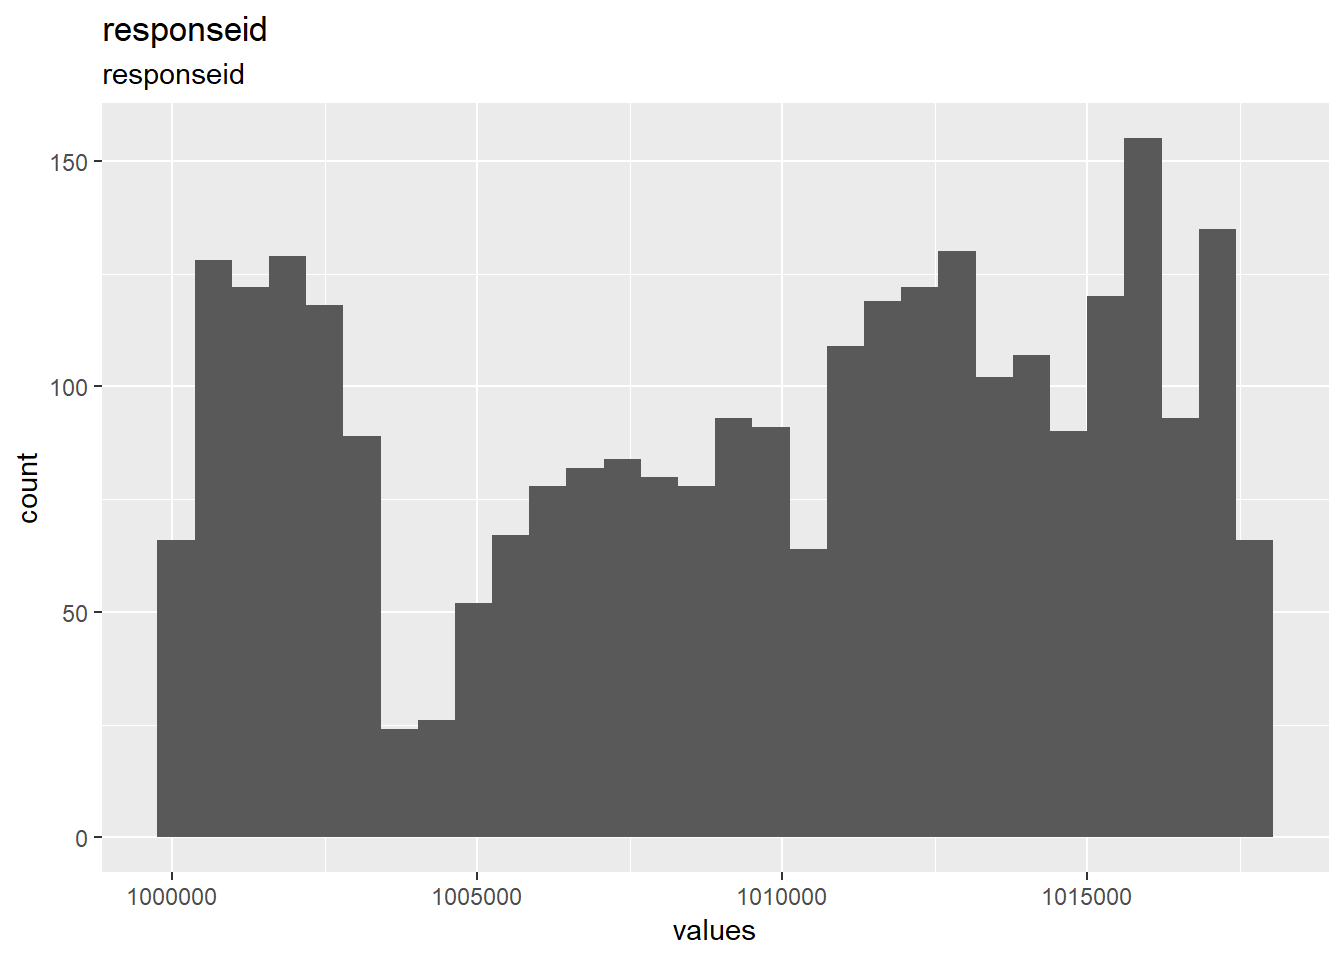
\includegraphics{Goodloser-appendix_files/figure-latex/responseid_distribution-1.pdf}

1 missings.

\subsubsection{Summary statistics}\label{responseid_summary}

name

label

data\_type

missing

complete

n

mean

sd

p0

p25

p50

p75

p100

hist

format.spss

responseid

responseid

numeric

1

17010

17011

1e+06

5074.32

1e+06

1e+06

1e+06

1e+06

1e+06

▇▇▇▇▇▇▇▇

F8.0

\subsection{r9pad1}\label{r9pad1}

How important is it to accept decisions about important social issues
adopted by politicians/authorities

\subsubsection{Distribution}\label{r9pad1_distribution}

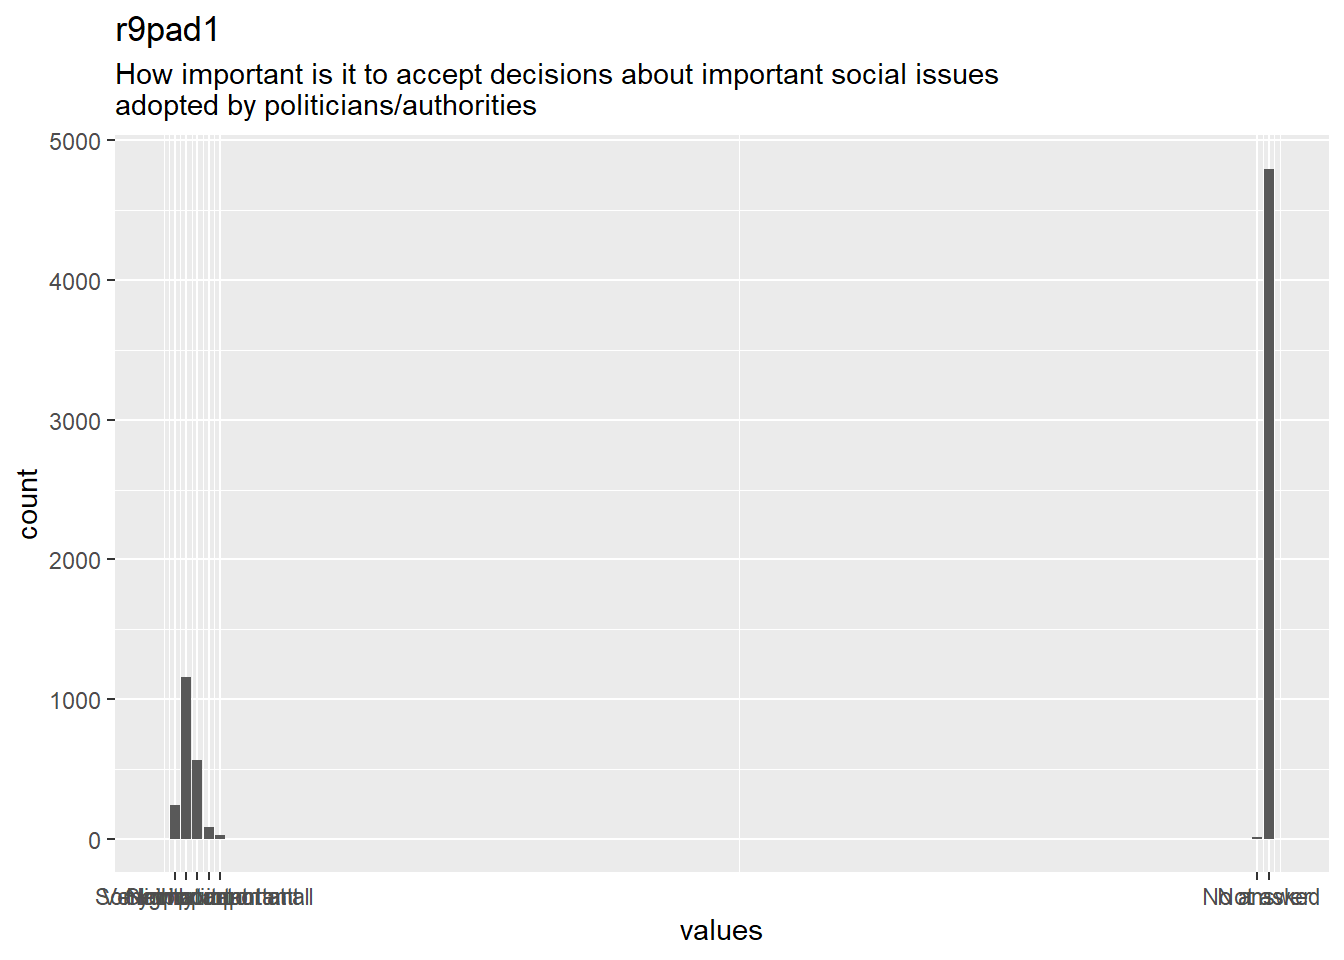
\includegraphics{Goodloser-appendix_files/figure-latex/r9pad1_distribution-1.pdf}

10114 missings.

\subsubsection{Summary statistics}\label{r9pad1_summary}

name

label

data\_type

value\_labels

missing

complete

n

mean

sd

p0

p25

p50

p75

p100

hist

format.spss

r9pad1

How important is it to accept decisions about important social issues
adopted by politicians/authorities

numeric

\begin{enumerate}
\def\labelenumi{\arabic{enumi}.}
\tightlist
\item
  Very important,2. Important,3. Somewhat important,4. Slightly
  important,5. Not important at all,97. No answer,98. Not asked

  10114

  6897

  17011

  69.1

  43.95

  1

  3

  98

  98

  98

  ▃▁▁▁▁▁▁▇

  F1.0
\end{enumerate}

\subsubsection{Value labels}\label{r9pad1_labels}

\begin{itemize}
\tightlist
\item
  \textbf{Very important}: \emph{1}
\item
  \textbf{Important}: \emph{2}
\item
  \textbf{Somewhat important}: \emph{3}
\item
  \textbf{Slightly important}: \emph{4}
\item
  \textbf{Not important at all}: \emph{5}
\item
  \textbf{No answer}: \emph{97}
\item
  \textbf{Not asked}: \emph{98}
\end{itemize}

\subsection{r9pad2}\label{r9pad2}

To what extent do people in Norway accept decisions about important
social issues adopted by politicians/authorities

\subsubsection{Distribution}\label{r9pad2_distribution}

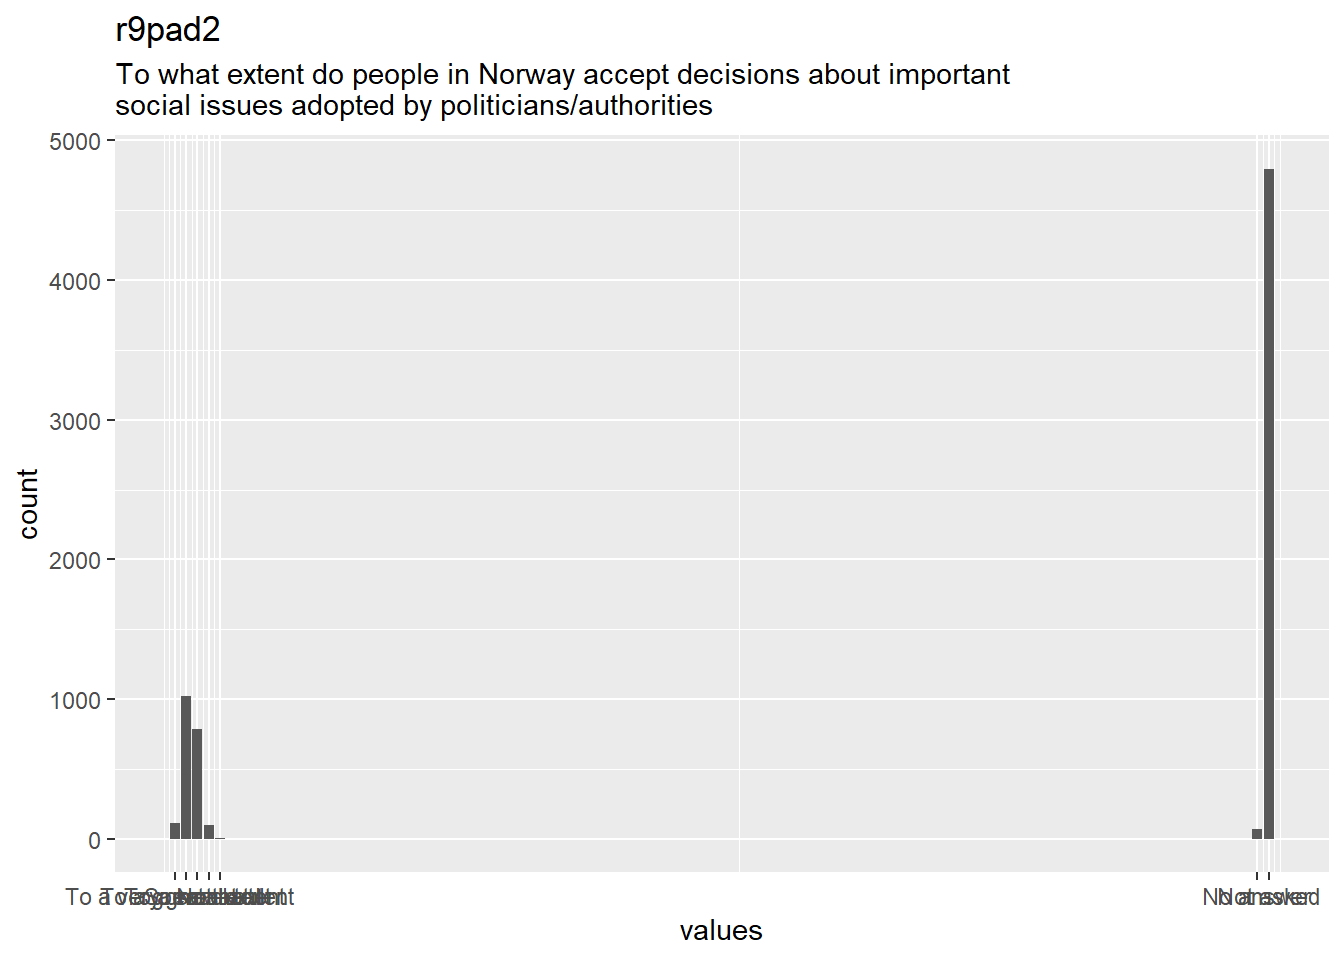
\includegraphics{Goodloser-appendix_files/figure-latex/r9pad2_distribution-1.pdf}

10114 missings.

\subsubsection{Summary statistics}\label{r9pad2_summary}

name

label

data\_type

value\_labels

missing

complete

n

mean

sd

p0

p25

p50

p75

p100

hist

format.spss

r9pad2

To what extent do people in Norway accept decisions about important
social issues adopted by politicians/authorities

numeric

\begin{enumerate}
\def\labelenumi{\arabic{enumi}.}
\tightlist
\item
  To a very great extent,2. To a great extent,3. Somewhat,4. To a small
  extent,5. Not at all,97. No answer,98. Not asked

  10114

  6897

  17011

  69.92

  43.52

  1

  3

  98

  98

  98

  ▃▁▁▁▁▁▁▇

  F1.0
\end{enumerate}

\subsubsection{Value labels}\label{r9pad2_labels}

\begin{itemize}
\tightlist
\item
  \textbf{To a very great extent}: \emph{1}
\item
  \textbf{To a great extent}: \emph{2}
\item
  \textbf{Somewhat}: \emph{3}
\item
  \textbf{To a small extent}: \emph{4}
\item
  \textbf{Not at all}: \emph{5}
\item
  \textbf{No answer}: \emph{97}
\item
  \textbf{Not asked}: \emph{98}
\end{itemize}

\subsection{r9pad3}\label{r9pad3}

Do you accept decisions about important social issues adopted by
politicians/authorities?

\subsubsection{Distribution}\label{r9pad3_distribution}

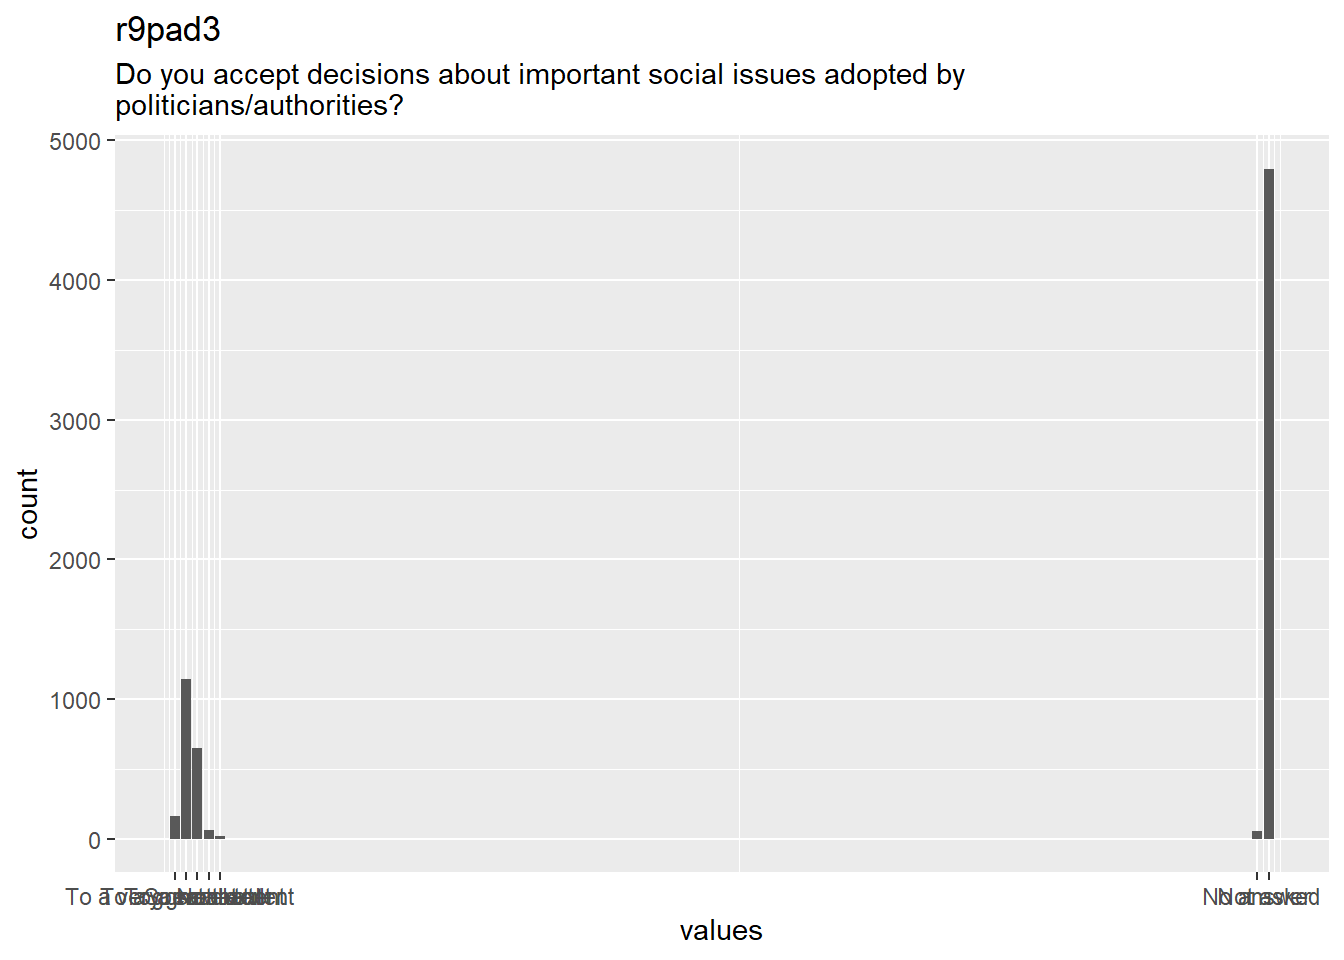
\includegraphics{Goodloser-appendix_files/figure-latex/r9pad3_distribution-1.pdf}

10114 missings.

\subsubsection{Summary statistics}\label{r9pad3_summary}

name

label

data\_type

value\_labels

missing

complete

n

mean

sd

p0

p25

p50

p75

p100

hist

format.spss

r9pad3

Do you accept decisions about important social issues adopted by
politicians/authorities?

numeric

\begin{enumerate}
\def\labelenumi{\arabic{enumi}.}
\tightlist
\item
  To a very great extent,2. To a great extent,3. Somewhat,4. To a small
  extent,5. Not at all,97. No answer,98. Not asked

  10114

  6897

  17011

  69.69

  43.66

  1

  3

  98

  98

  98

  ▃▁▁▁▁▁▁▇

  F1.0
\end{enumerate}

\subsubsection{Value labels}\label{r9pad3_labels}

\begin{itemize}
\tightlist
\item
  \textbf{To a very great extent}: \emph{1}
\item
  \textbf{To a great extent}: \emph{2}
\item
  \textbf{Somewhat}: \emph{3}
\item
  \textbf{To a small extent}: \emph{4}
\item
  \textbf{Not at all}: \emph{5}
\item
  \textbf{No answer}: \emph{97}
\item
  \textbf{Not asked}: \emph{98}
\end{itemize}

\subsection{r10panelpad}\label{r10panelpad}

{[}Defines sub-group: panelpad. These are respondents who have responded
to R9PAD1-3 but where u!=4{]}

\subsubsection{Distribution}\label{r10panelpad_distribution}

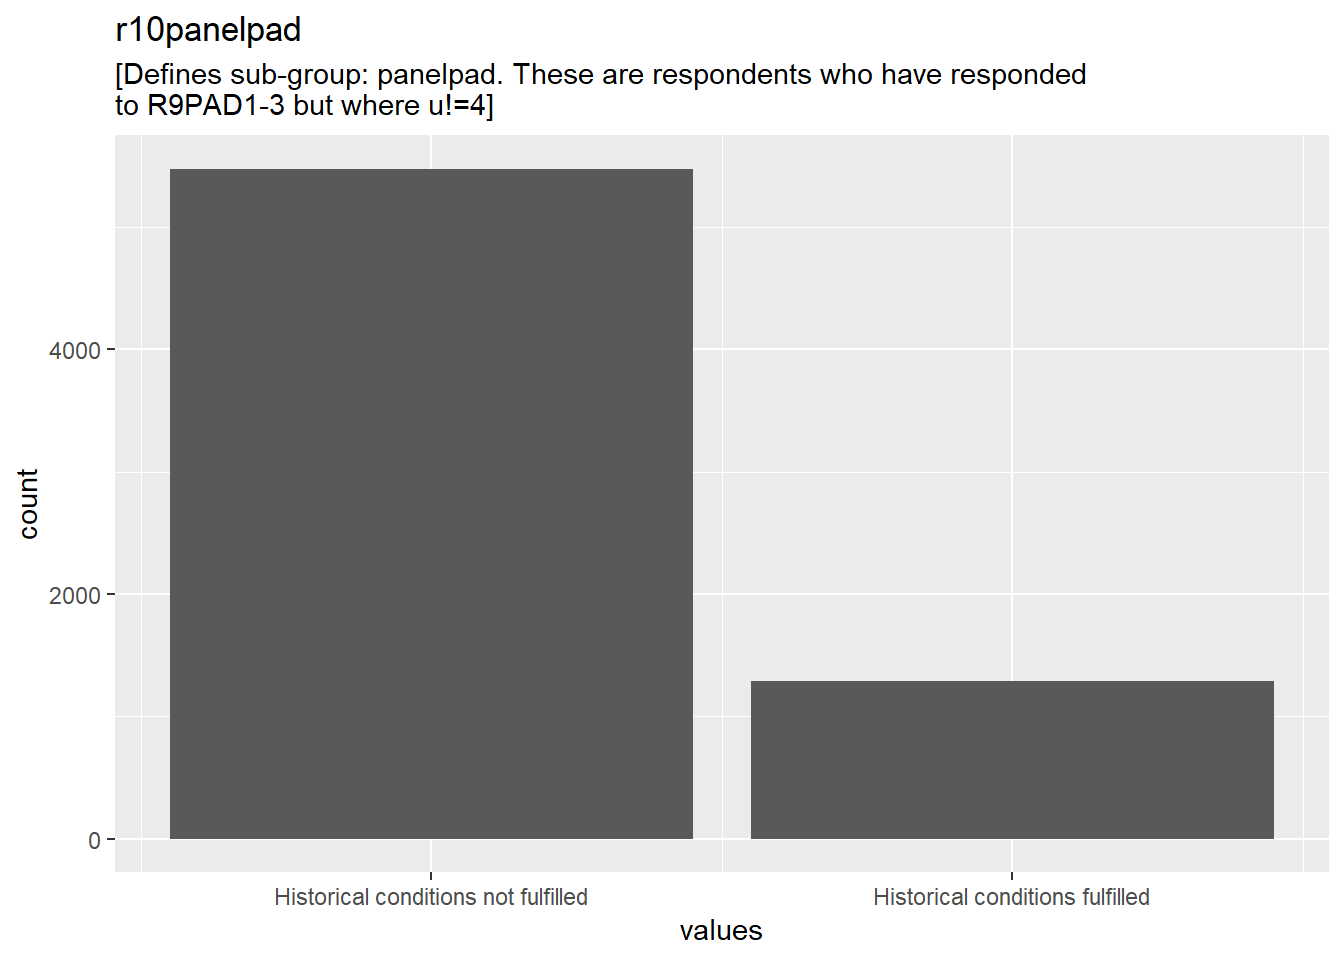
\includegraphics{Goodloser-appendix_files/figure-latex/r10panelpad_distribution-1.pdf}

10246 missings.

\subsubsection{Summary statistics}\label{r10panelpad_summary}

name

label

data\_type

value\_labels

missing

complete

n

mean

sd

p0

p25

p50

p75

p100

hist

format.spss

r10panelpad

{[}Defines sub-group: panelpad. These are respondents who have responded
to R9PAD1-3 but where u!=4{]}

numeric

\begin{enumerate}
\def\labelenumi{\arabic{enumi}.}
\setcounter{enumi}{-1}
\tightlist
\item
  Historical conditions not fulfilled,1. Historical conditions fulfilled

  10246

  6765

  17011

  0.19

  0.39

  0

  0

  0

  0

  1

  ▇▁▁▁▁▁▁▂

  F1.0
\end{enumerate}

\subsubsection{Value labels}\label{r10panelpad_labels}

\begin{itemize}
\tightlist
\item
  \textbf{Historical conditions not fulfilled}: \emph{0}
\item
  \textbf{Historical conditions fulfilled}: \emph{1}
\end{itemize}

\subsection{r10pad1}\label{r10pad1}

Opinion on begging ban in your municipality.

\subsubsection{Distribution}\label{r10pad1_distribution}

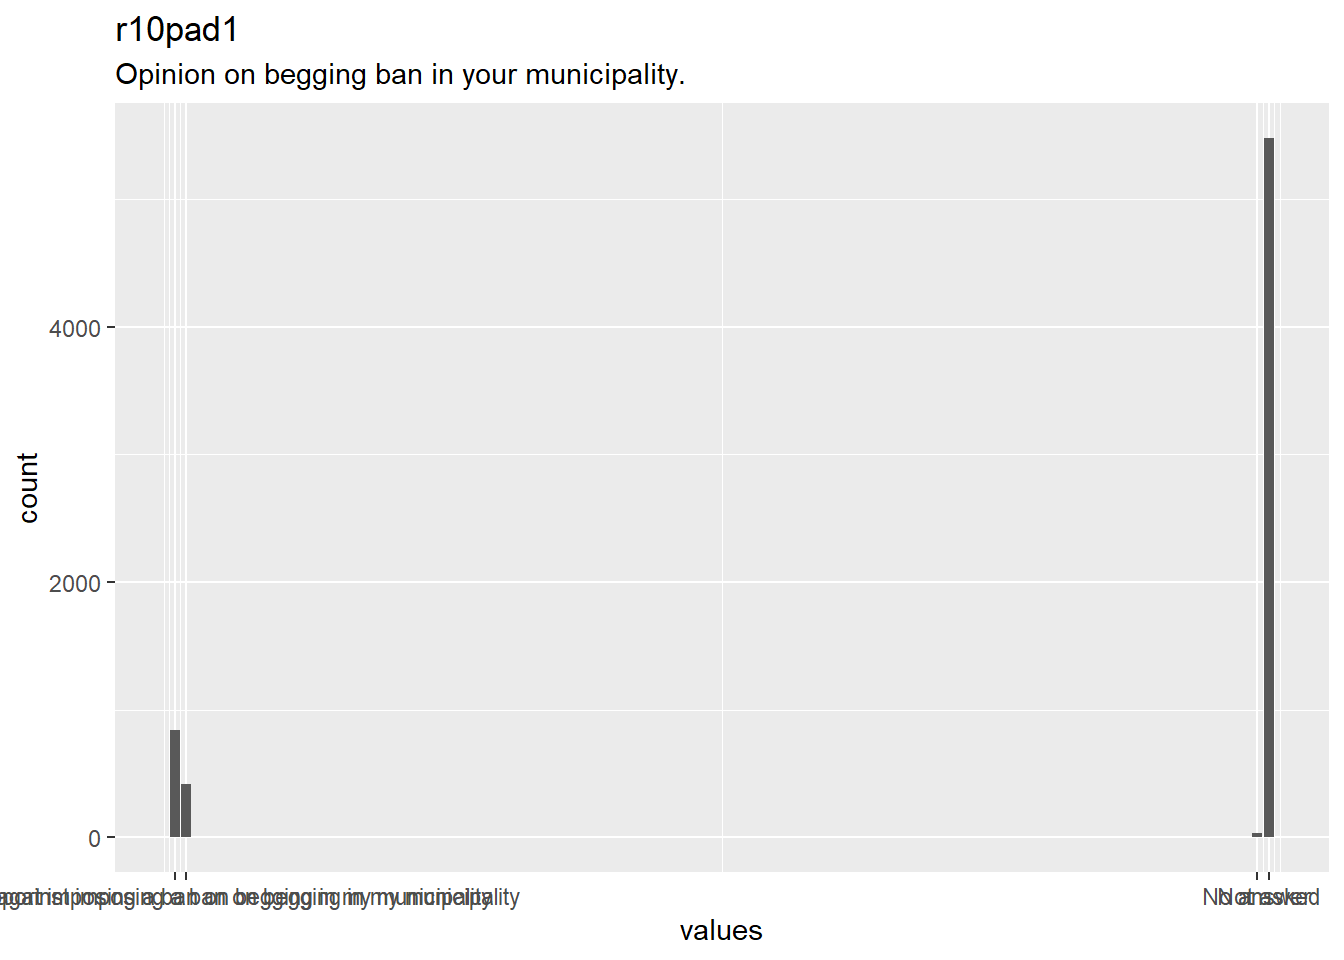
\includegraphics{Goodloser-appendix_files/figure-latex/r10pad1_distribution-1.pdf}

10246 missings.

\subsubsection{Summary statistics}\label{r10pad1_summary}

name

label

data\_type

value\_labels

missing

complete

n

mean

sd

p0

p25

p50

p75

p100

hist

format.spss

r10pad1

Opinion on begging ban in your municipality.

numeric

\begin{enumerate}
\def\labelenumi{\arabic{enumi}.}
\tightlist
\item
  I generally support imposing a ban on begging in my municipality,2. I
  am generally against imposing a ban on begging in my municipality,97.
  No answer,98. Not asked

  10246

  6765

  17011

  80.03

  37.6

  1

  98

  98

  98

  98

  ▂▁▁▁▁▁▁▇

  F1.0
\end{enumerate}

\subsubsection{Value labels}\label{r10pad1_labels}

\begin{itemize}
\tightlist
\item
  \textbf{I generally support imposing a ban on begging in my
  municipality}: \emph{1}
\item
  \textbf{I am generally against imposing a ban on begging in my
  municipality}: \emph{2}
\item
  \textbf{No answer}: \emph{97}
\item
  \textbf{Not asked}: \emph{98}
\end{itemize}

\subsection{r10pad2}\label{r10pad2}

How important is a begging ban for you.

\subsubsection{Distribution}\label{r10pad2_distribution}

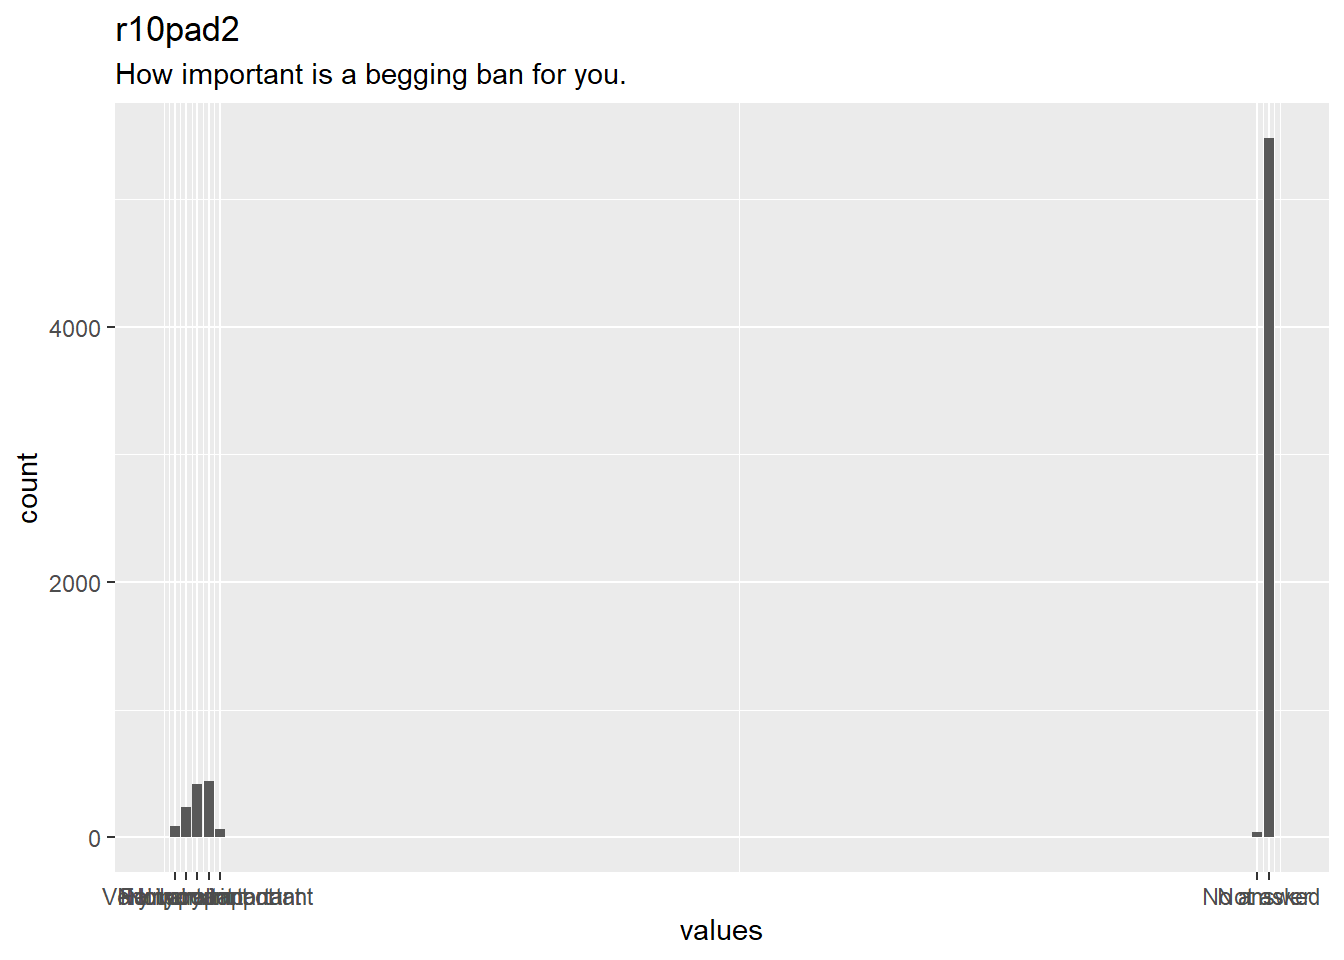
\includegraphics{Goodloser-appendix_files/figure-latex/r10pad2_distribution-1.pdf}

10246 missings.

\subsubsection{Summary statistics}\label{r10pad2_summary}

name

label

data\_type

value\_labels

missing

complete

n

mean

sd

p0

p25

p50

p75

p100

hist

format.spss

r10pad2

How important is a begging ban for you.

numeric

\begin{enumerate}
\def\labelenumi{\arabic{enumi}.}
\tightlist
\item
  Very important,2. Important,3. Fairly important,4. Not very
  important,5. Not at all important,97. No answer,98. Not asked

  10246

  6765

  17011

  80.45

  36.83

  1

  98

  98

  98

  98

  ▂▁▁▁▁▁▁▇

  F1.0
\end{enumerate}

\subsubsection{Value labels}\label{r10pad2_labels}

\begin{itemize}
\tightlist
\item
  \textbf{Very important}: \emph{1}
\item
  \textbf{Important}: \emph{2}
\item
  \textbf{Fairly important}: \emph{3}
\item
  \textbf{Not very important}: \emph{4}
\item
  \textbf{Not at all important}: \emph{5}
\item
  \textbf{No answer}: \emph{97}
\item
  \textbf{Not asked}: \emph{98}
\end{itemize}

\subsection{r10pad3\_mobil}\label{r10pad3_mobil}

{[}Asked if panelPAD=1. Background variable for r10pad3 (video). Detects
whether or not the respondent is using a mobile device{]}

\subsubsection{Distribution}\label{r10pad3_mobil_distribution}

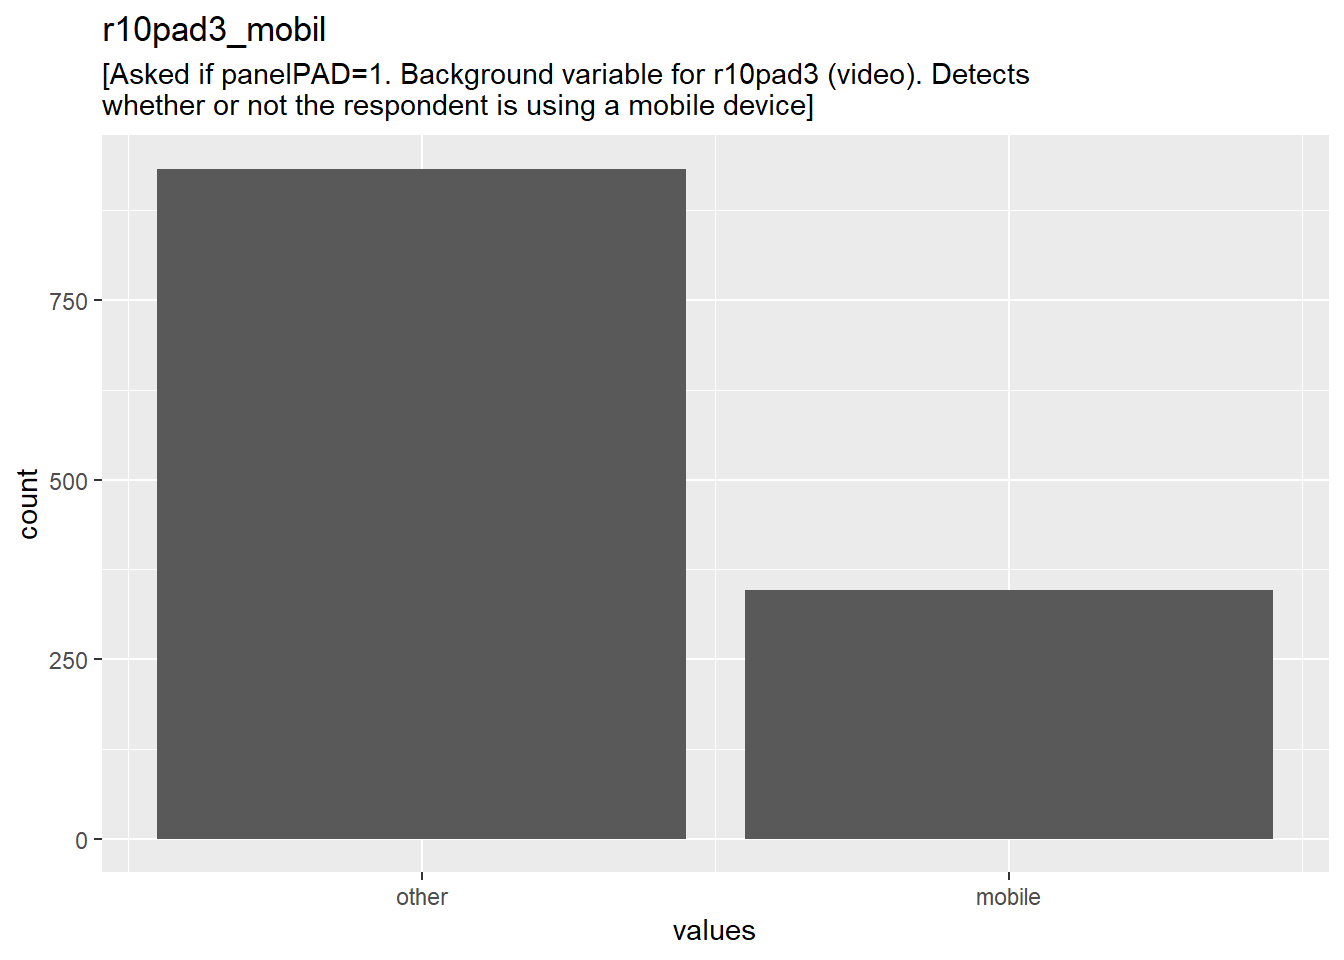
\includegraphics{Goodloser-appendix_files/figure-latex/r10pad3_mobil_distribution-1.pdf}

15732 missings.

\subsubsection{Summary statistics}\label{r10pad3_mobil_summary}

name

label

data\_type

value\_labels

missing

complete

n

mean

sd

p0

p25

p50

p75

p100

hist

format.spss

r10pad3\_mobil

{[}Asked if panelPAD=1. Background variable for r10pad3 (video). Detects
whether or not the respondent is using a mobile device{]}

numeric

\begin{enumerate}
\def\labelenumi{\arabic{enumi}.}
\setcounter{enumi}{-1}
\tightlist
\item
  other,1. mobile

  15732

  1279

  17011

  0.27

  0.44

  0

  0

  0

  1

  1

  ▇▁▁▁▁▁▁▃

  F1.0
\end{enumerate}

\subsubsection{Value labels}\label{r10pad3_mobil_labels}

\begin{itemize}
\tightlist
\item
  \textbf{other}: \emph{0}
\item
  \textbf{mobile}: \emph{1}
\end{itemize}

\subsection{r10pad3a\_ran}\label{r10pad3a_ran}

{[}Randomizes if panelPAD=1. Background variable for r10pad3 (video).
Respondents who chose option 2 in r10pad1 gets one of the 5 r10pad3B
variants, randomly selected. Respondents who got r10pad1 but skipped the
question gets randomly assigned one of the 10

\subsubsection{Distribution}\label{r10pad3a_ran_distribution}

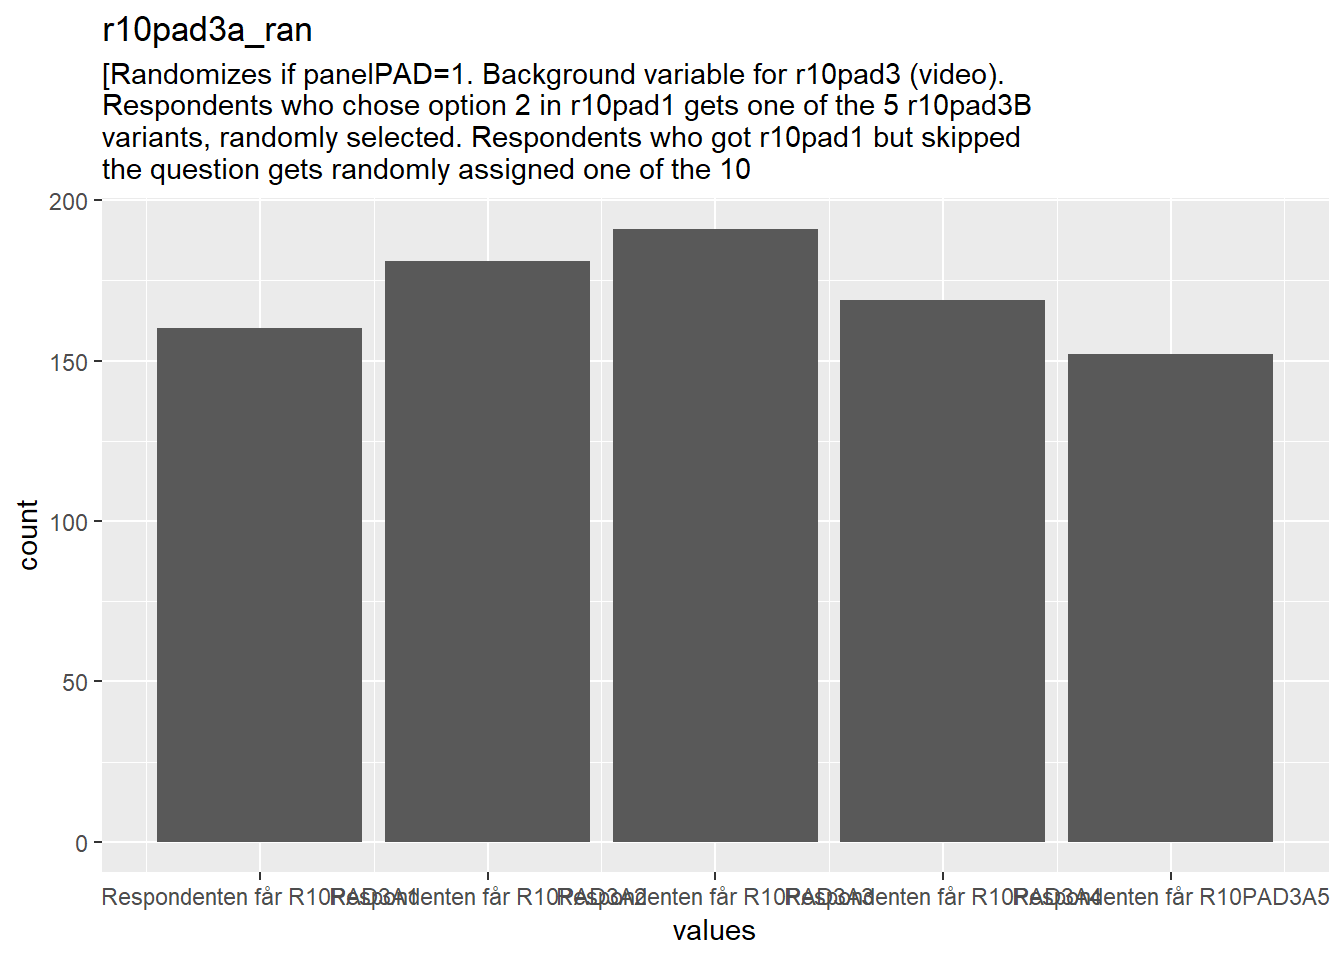
\includegraphics{Goodloser-appendix_files/figure-latex/r10pad3a_ran_distribution-1.pdf}

16158 missings.

\subsubsection{Summary statistics}\label{r10pad3a_ran_summary}

name

label

data\_type

value\_labels

missing

complete

n

mean

sd

p0

p25

p50

p75

p100

hist

format.spss

r10pad3a\_ran

{[}Randomizes if panelPAD=1. Background variable for r10pad3 (video).
Respondents who chose option 2 in r10pad1 gets one of the 5 r10pad3B
variants, randomly selected. Respondents who got r10pad1 but skipped the
question gets randomly assigned one of the 10

numeric

\begin{enumerate}
\def\labelenumi{\arabic{enumi}.}
\tightlist
\item
  Respondenten får R10PAD3A1,2. Respondenten får R10PAD3A2,3.
  Respondenten får R10PAD3A3,4. Respondenten får R10PAD3A4,5.
  Respondenten får R10PAD3A5

  16158

  853

  17011

  2.97

  1.37

  1

  2

  3

  4

  5

  ▇▇▁▇▁▇▁▆

  F1.0
\end{enumerate}

\subsubsection{Value labels}\label{r10pad3a_ran_labels}

\begin{itemize}
\tightlist
\item
  \textbf{Respondenten får R10PAD3A1}: \emph{1}
\item
  \textbf{Respondenten får R10PAD3A2}: \emph{2}
\item
  \textbf{Respondenten får R10PAD3A3}: \emph{3}
\item
  \textbf{Respondenten får R10PAD3A4}: \emph{4}
\item
  \textbf{Respondenten får R10PAD3A5}: \emph{5}
\end{itemize}

\subsection{r10pad3b\_ran}\label{r10pad3b_ran}

{[}Randomizes if panelPAD=1. Background variable for r10pad3 (video).
Respondents who chose option 2 in r10pad1 gets one of the 5 r10pad3B
variants, randomly selected. Respondents who got r10pad1 but skipped the
question gets randomly assigned one of the 10

\subsubsection{Distribution}\label{r10pad3b_ran_distribution}

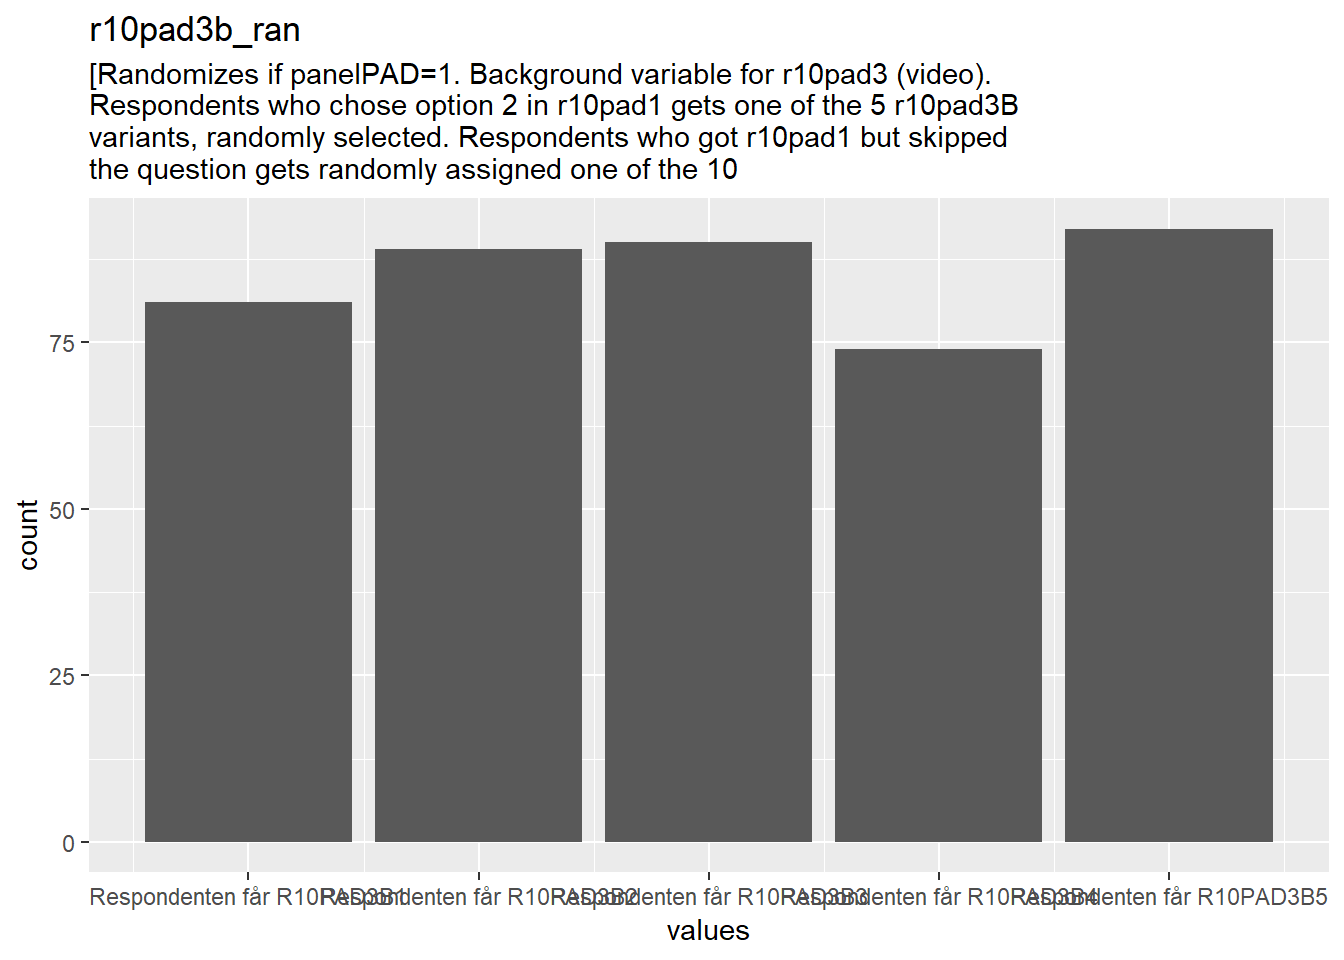
\includegraphics{Goodloser-appendix_files/figure-latex/r10pad3b_ran_distribution-1.pdf}

16585 missings.

\subsubsection{Summary statistics}\label{r10pad3b_ran_summary}

name

label

data\_type

value\_labels

missing

complete

n

mean

sd

p0

p25

p50

p75

p100

hist

format.spss

r10pad3b\_ran

{[}Randomizes if panelPAD=1. Background variable for r10pad3 (video).
Respondents who chose option 2 in r10pad1 gets one of the 5 r10pad3B
variants, randomly selected. Respondents who got r10pad1 but skipped the
question gets randomly assigned one of the 10

numeric

\begin{enumerate}
\def\labelenumi{\arabic{enumi}.}
\tightlist
\item
  Respondenten får R10PAD3B1,2. Respondenten får R10PAD3B2,3.
  Respondenten får R10PAD3B3,4. Respondenten får R10PAD3B4,5.
  Respondenten får R10PAD3B5

  16585

  426

  17011

  3.02

  1.42

  1

  2

  3

  4

  5

  ▇▇▁▇▁▆▁▇

  F1.0
\end{enumerate}

\subsubsection{Value labels}\label{r10pad3b_ran_labels}

\begin{itemize}
\tightlist
\item
  \textbf{Respondenten får R10PAD3B1}: \emph{1}
\item
  \textbf{Respondenten får R10PAD3B2}: \emph{2}
\item
  \textbf{Respondenten får R10PAD3B3}: \emph{3}
\item
  \textbf{Respondenten får R10PAD3B4}: \emph{4}
\item
  \textbf{Respondenten får R10PAD3B5}: \emph{5}
\end{itemize}

\subsection{r10pad3ended}\label{r10pad3ended}

{[}Asked if panelPAD=1. Background variable for r10pad3 (video). Counter
for the event ``video ended''{]}

\subsubsection{Distribution}\label{r10pad3ended_distribution}

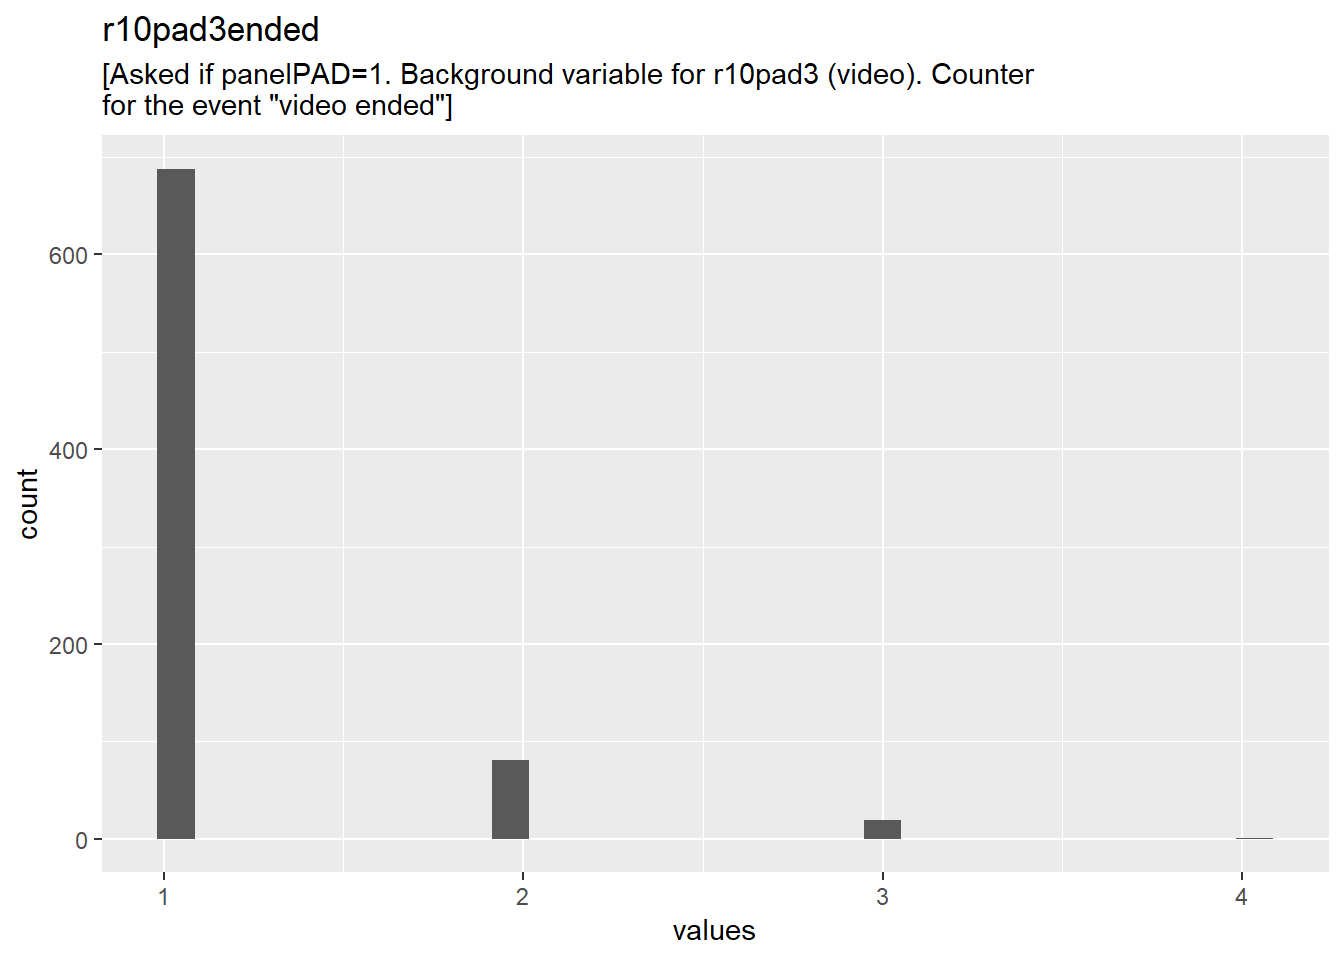
\includegraphics{Goodloser-appendix_files/figure-latex/r10pad3ended_distribution-1.pdf}

16222 missings.

\subsubsection{Summary statistics}\label{r10pad3ended_summary}

name

label

data\_type

missing

complete

n

mean

sd

p0

p25

p50

p75

p100

hist

format.spss

r10pad3ended

{[}Asked if panelPAD=1. Background variable for r10pad3 (video). Counter
for the event ``video ended''{]}

numeric

16222

789

17011

1.15

0.43

1

1

1

1

4

▇▁▁▁▁▁▁▁

F20.0

\subsection{r10pad3error}\label{r10pad3error}

{[}Asked if panelPAD=1. Background variable for r10pad3 (video). Counter
for the event ``video error''{]}

\subsubsection{Distribution}\label{r10pad3error_distribution}

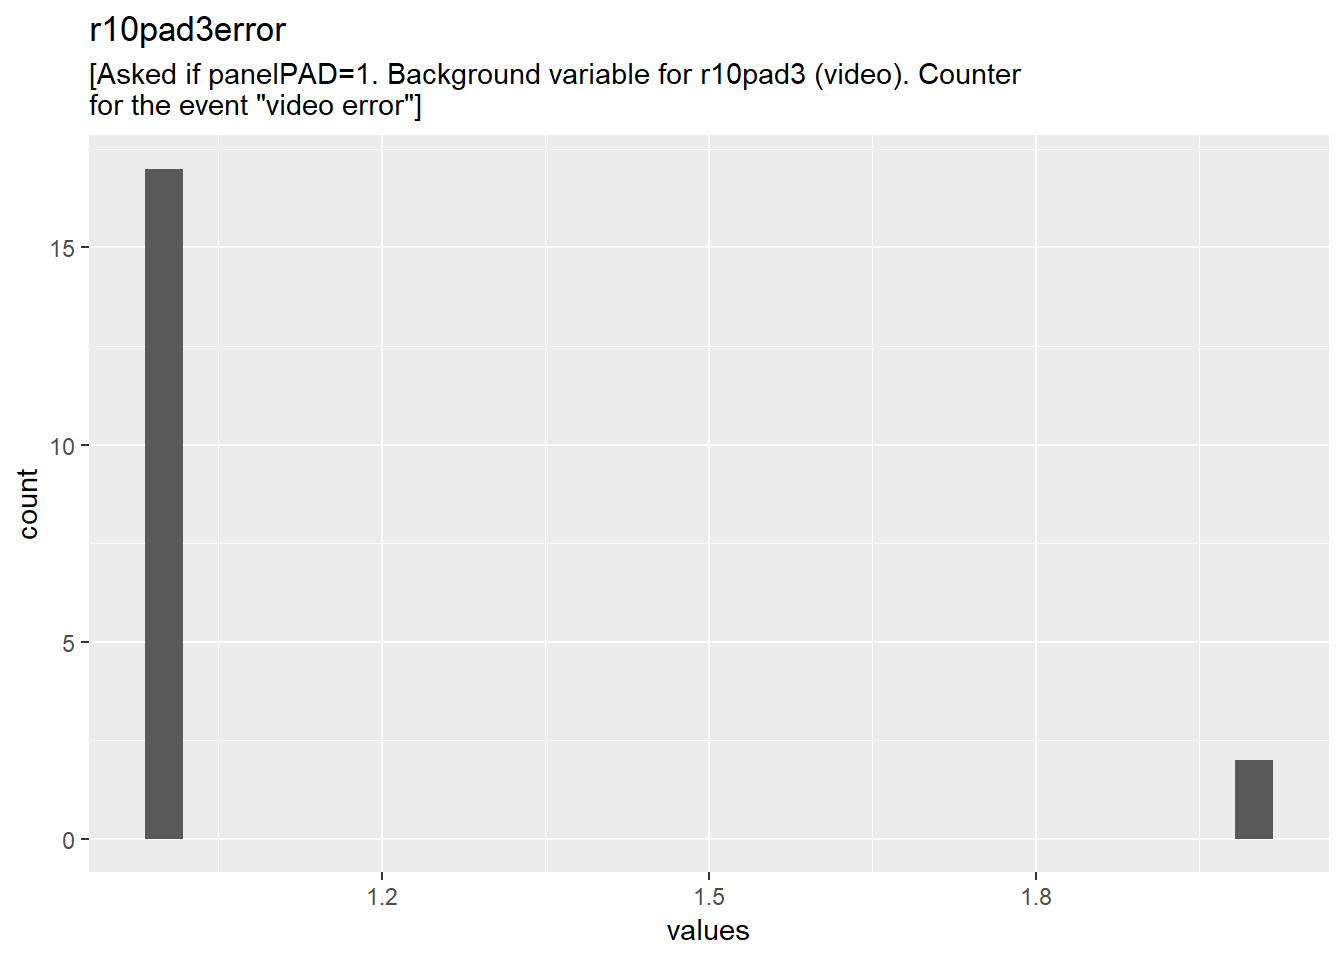
\includegraphics{Goodloser-appendix_files/figure-latex/r10pad3error_distribution-1.pdf}

16992 missings.

\subsubsection{Summary statistics}\label{r10pad3error_summary}

name

label

data\_type

missing

complete

n

mean

sd

p0

p25

p50

p75

p100

hist

format.spss

r10pad3error

{[}Asked if panelPAD=1. Background variable for r10pad3 (video). Counter
for the event ``video error''{]}

numeric

16992

19

17011

1.11

0.32

1

1

1

1

2

▇▁▁▁▁▁▁▁

F20.0

\subsection{r10pad3paused}\label{r10pad3paused}

{[}Asked if panelPAD=1. Background variable for r10pad3 (video). Counter
for the event ``video paused''{]}

\subsubsection{Distribution}\label{r10pad3paused_distribution}

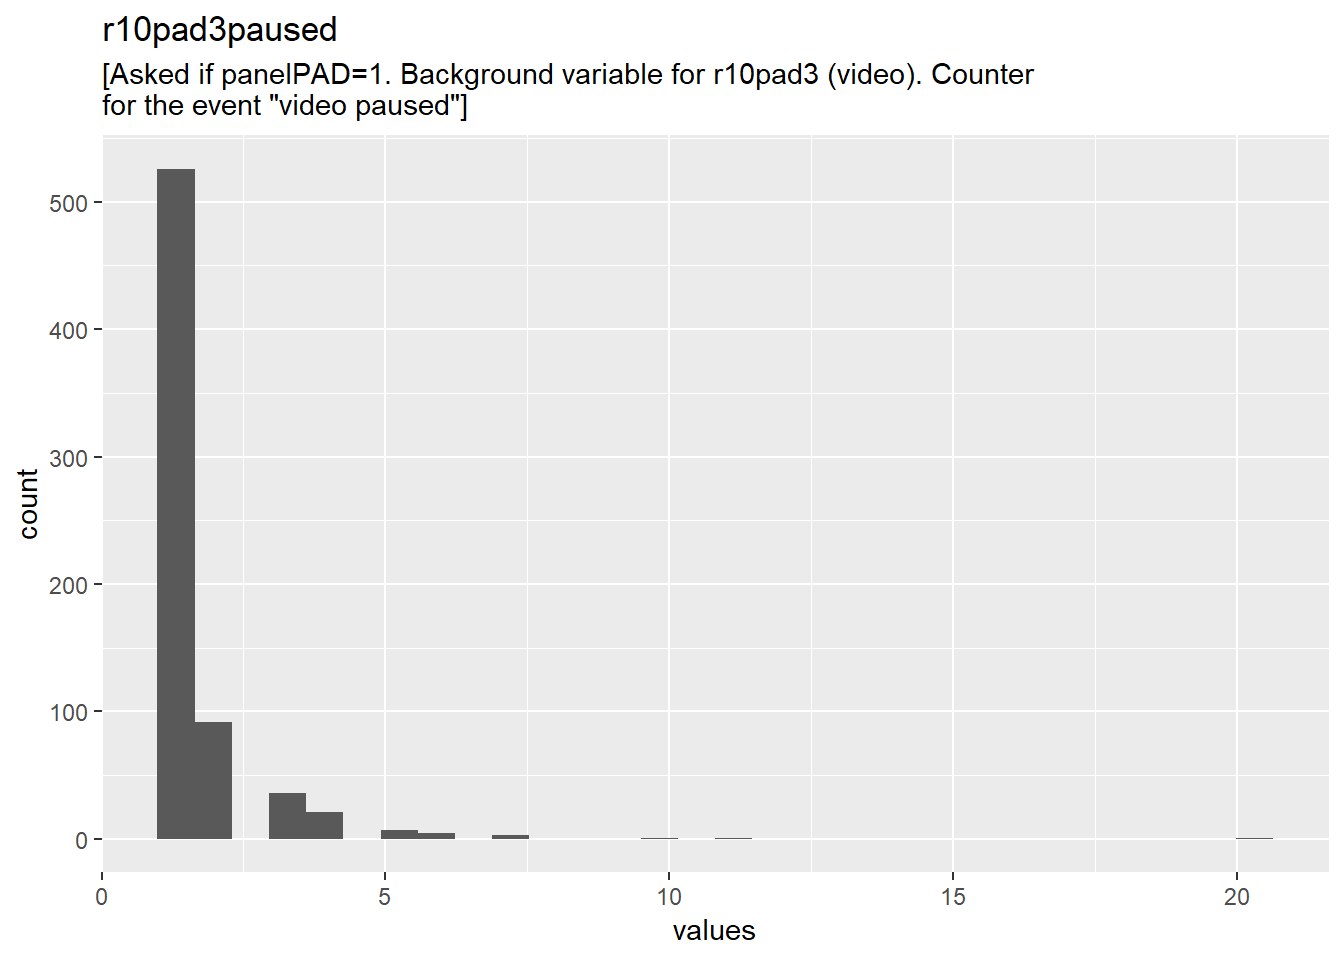
\includegraphics{Goodloser-appendix_files/figure-latex/r10pad3paused_distribution-1.pdf}

16318 missings.

\subsubsection{Summary statistics}\label{r10pad3paused_summary}

name

label

data\_type

missing

complete

n

mean

sd

p0

p25

p50

p75

p100

hist

format.spss

r10pad3paused

{[}Asked if panelPAD=1. Background variable for r10pad3 (video). Counter
for the event ``video paused''{]}

numeric

16318

693

17011

1.48

1.29

1

1

1

1

20

▇▁▁▁▁▁▁▁

F20.0

\subsection{r10pad3played}\label{r10pad3played}

{[}Asked if panelPAD=1. Background variable for r10pad3 (video). Counter
for the event ``video played''{]}

\subsubsection{Distribution}\label{r10pad3played_distribution}

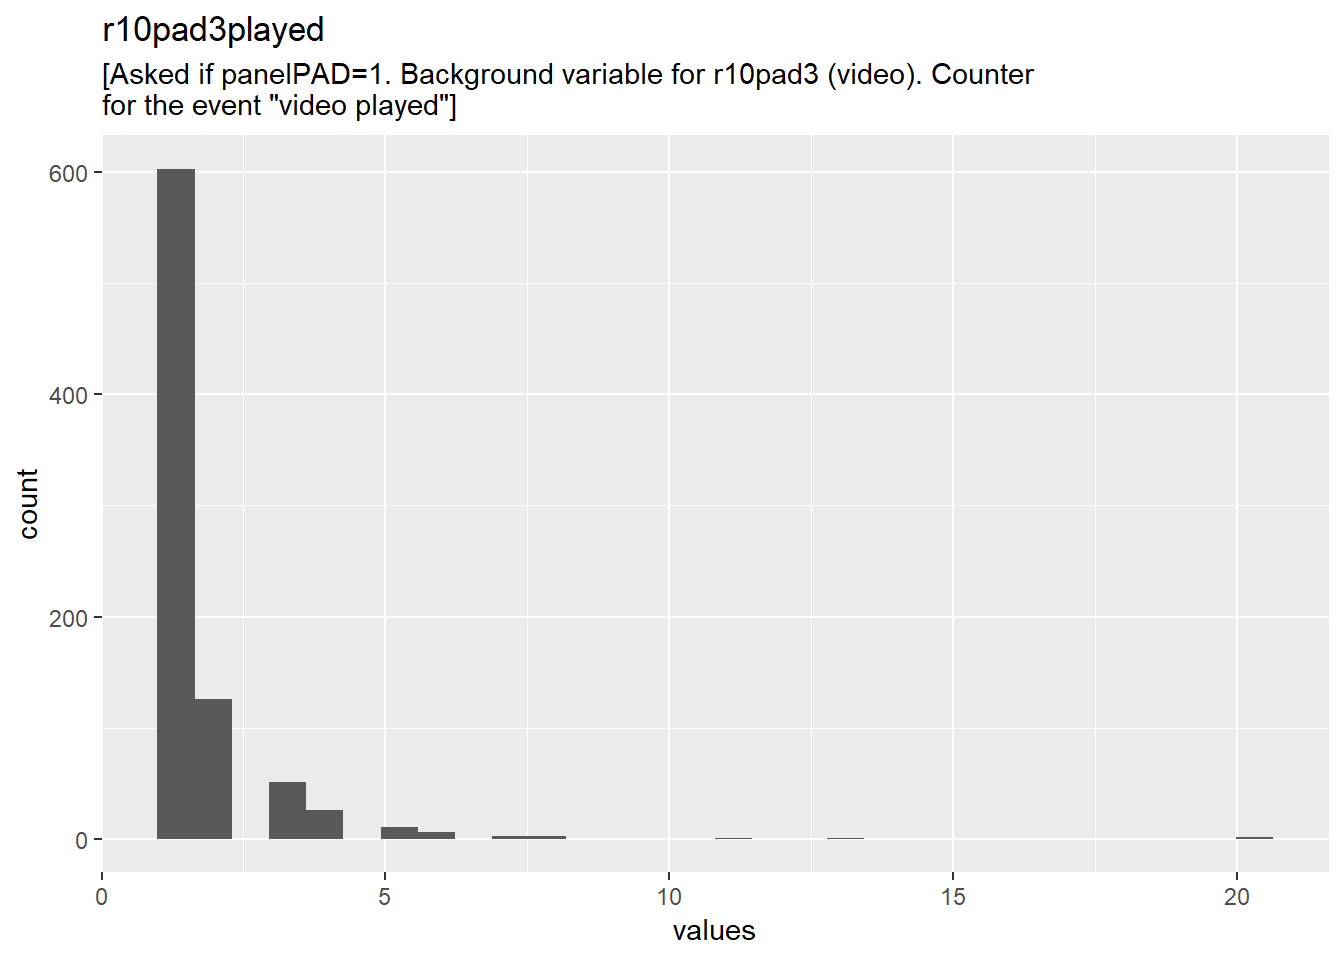
\includegraphics{Goodloser-appendix_files/figure-latex/r10pad3played_distribution-1.pdf}

16178 missings.

\subsubsection{Summary statistics}\label{r10pad3played_summary}

name

label

data\_type

missing

complete

n

mean

sd

p0

p25

p50

p75

p100

hist

format.spss

r10pad3played

{[}Asked if panelPAD=1. Background variable for r10pad3 (video). Counter
for the event ``video played''{]}

numeric

16178

833

17011

1.58

1.49

1

1

1

2

20

▇▁▁▁▁▁▁▁

F20.0

\subsection{r10pad3\_timespent}\label{r10pad3_timespent}

{[}Asked if panelPAD=1. Background variable for r10pad3 (video).
Calculated time spent in the video node{]}

\subsubsection{Distribution}\label{r10pad3_timespent_distribution}

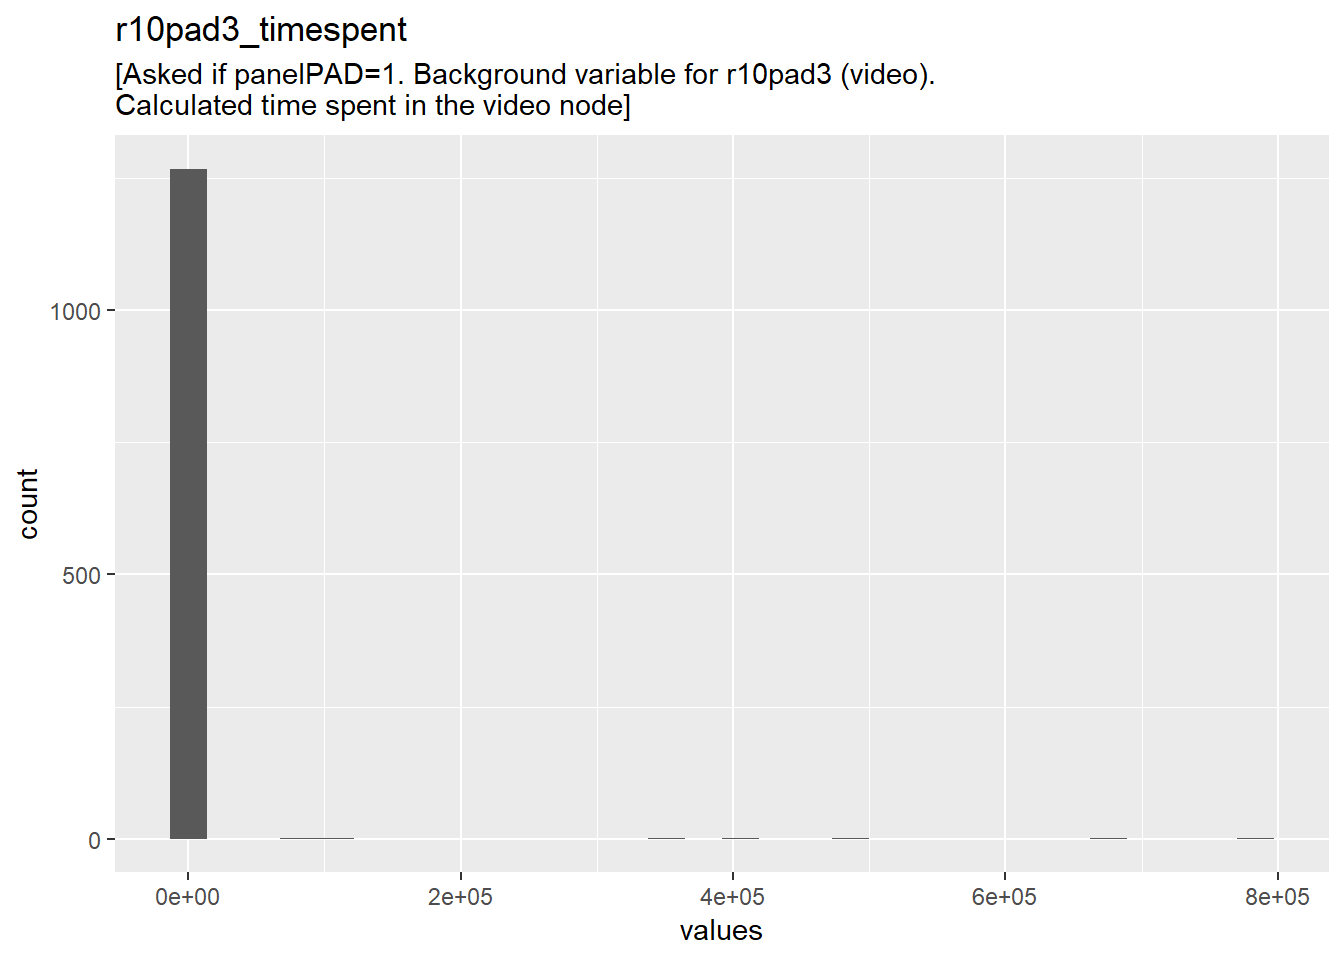
\includegraphics{Goodloser-appendix_files/figure-latex/r10pad3_timespent_distribution-1.pdf}

15737 missings.

\subsubsection{Summary statistics}\label{r10pad3_timespent_summary}

name

label

data\_type

missing

complete

n

mean

sd

p0

p25

p50

p75

p100

hist

format.spss

r10pad3\_timespent

{[}Asked if panelPAD=1. Background variable for r10pad3 (video).
Calculated time spent in the video node{]}

numeric

15737

1274

17011

2440.89

35767.62

2

94

109

124

783439

▇▁▁▁▁▁▁▁

F20.0

\subsection{r10pad4}\label{r10pad4}

What was the recording like?

\subsubsection{Distribution}\label{r10pad4_distribution}

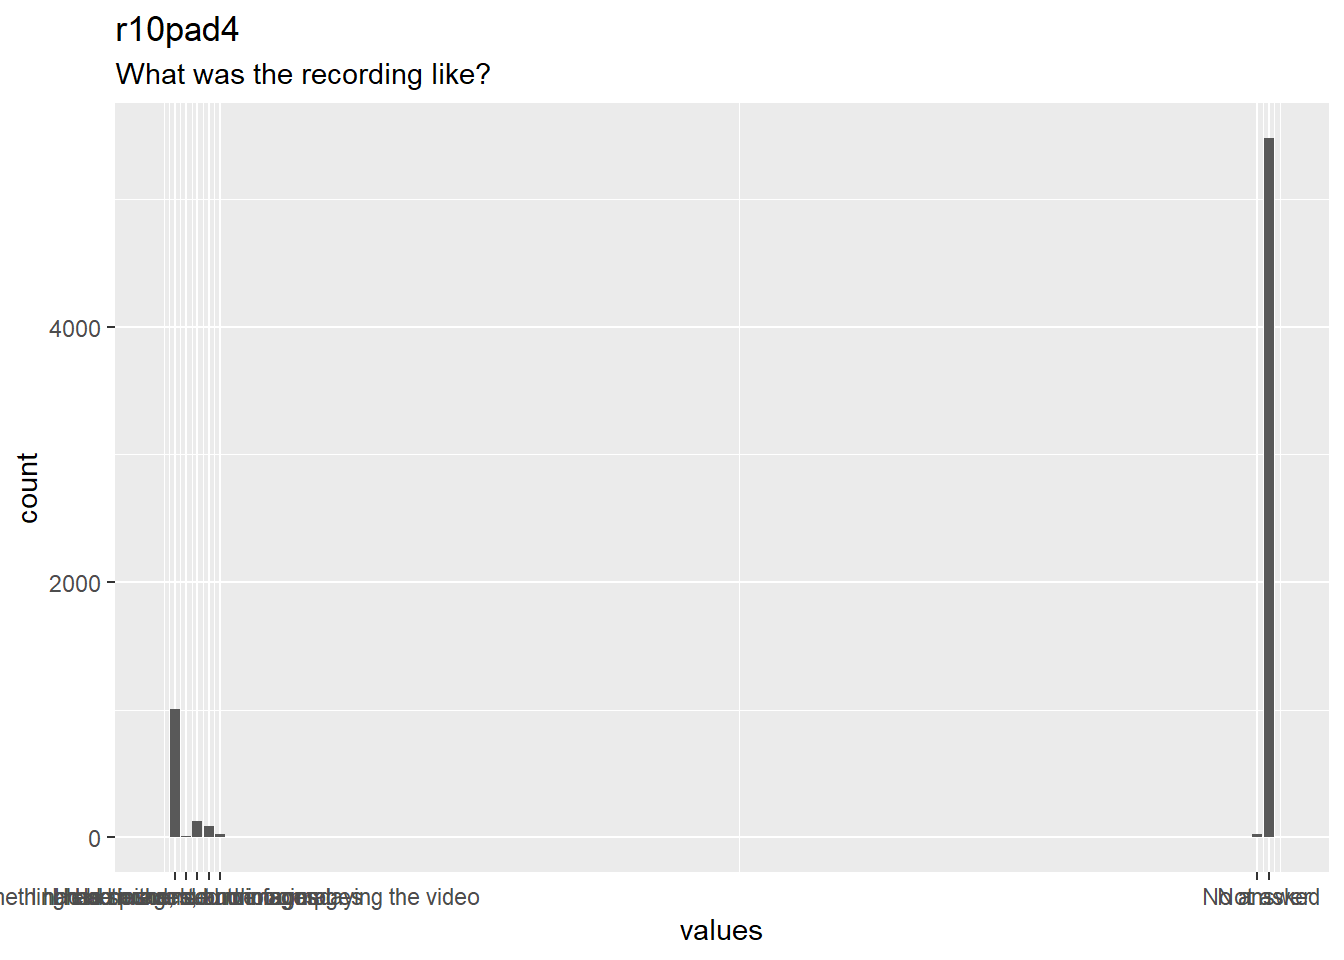
\includegraphics{Goodloser-appendix_files/figure-latex/r10pad4_distribution-1.pdf}

10246 missings.

\subsubsection{Summary statistics}\label{r10pad4_summary}

name

label

data\_type

value\_labels

missing

complete

n

mean

sd

p0

p25

p50

p75

p100

hist

format.spss

r10pad4

What was the recording like?

numeric

\begin{enumerate}
\def\labelenumi{\arabic{enumi}.}
\tightlist
\item
  I had both sound and images,2. I had sound, but no images,3. I had
  images, but no sound,4. I had neither sound nor images,5. Something
  else prevented me from playing the video,97. No answer,98. Not asked

  10246

  6765

  17011

  79.98

  37.6

  1

  98

  98

  98

  98

  ▂▁▁▁▁▁▁▇

  F1.0
\end{enumerate}

\subsubsection{Value labels}\label{r10pad4_labels}

\begin{itemize}
\tightlist
\item
  \textbf{I had both sound and images}: \emph{1}
\item
  \textbf{I had sound, but no images}: \emph{2}
\item
  \textbf{I had images, but no sound}: \emph{3}
\item
  \textbf{I had neither sound nor images}: \emph{4}
\item
  \textbf{Something else prevented me from playing the video}: \emph{5}
\item
  \textbf{No answer}: \emph{97}
\item
  \textbf{Not asked}: \emph{98}
\end{itemize}

\subsection{r10pad4\_comment}\label{r10pad4_comment}

Comments about the recording. {[}Data withheld for the sake of
anonymity{]}

\subsubsection{Distribution}\label{r10pad4_comment_distribution}

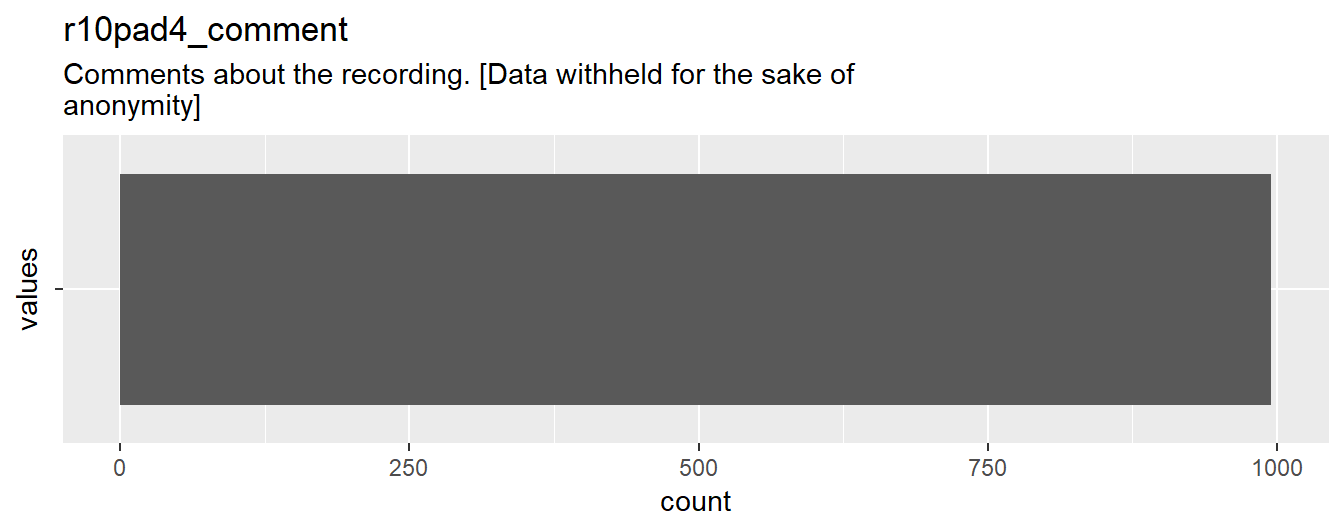
\includegraphics{Goodloser-appendix_files/figure-latex/r10pad4_comment_distribution-1.pdf}

0 missings.

\subsubsection{Summary statistics}\label{r10pad4_comment_summary}

name

label

data\_type

missing

complete

n

empty

n\_unique

min

max

format.spss

display\_width

r10pad4\_comment

Comments about the recording. {[}Data withheld for the sake of
anonymity{]}

character

0

17011

17011

17011

1

0

0

A1

1

\subsection{r10pad5}\label{r10pad5}

How fair was the way the decision was made.

\subsubsection{Distribution}\label{r10pad5_distribution}

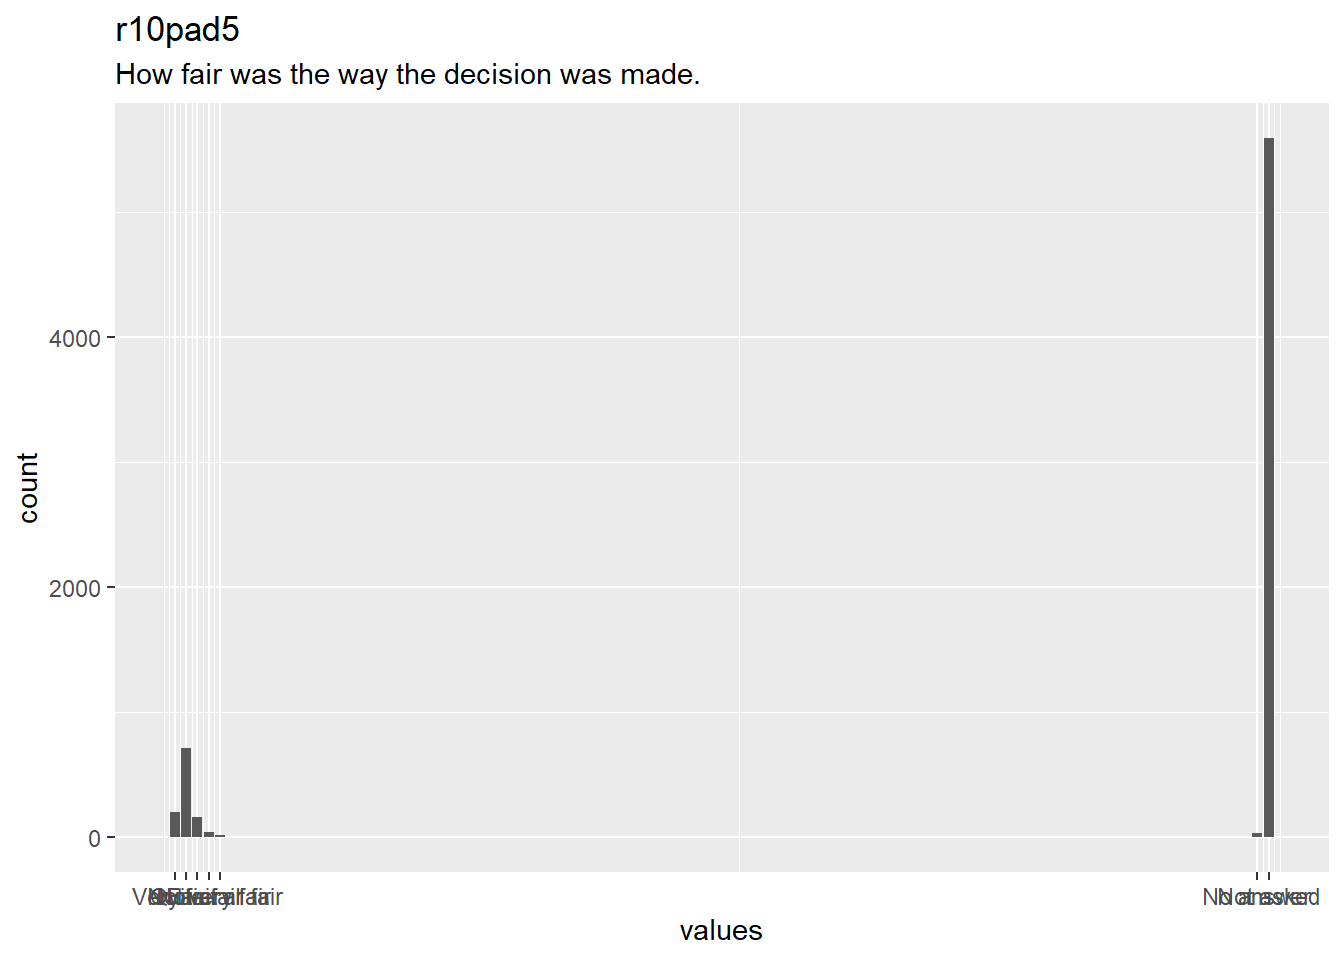
\includegraphics{Goodloser-appendix_files/figure-latex/r10pad5_distribution-1.pdf}

10246 missings.

\subsubsection{Summary statistics}\label{r10pad5_summary}

name

label

data\_type

value\_labels

missing

complete

n

mean

sd

p0

p25

p50

p75

p100

hist

format.spss

r10pad5

How fair was the way the decision was made.

numeric

\begin{enumerate}
\def\labelenumi{\arabic{enumi}.}
\tightlist
\item
  Very fair,2. Fair,3. Quite fair,4. Not very fair,5. Not at all
  fair,97. No answer,98. Not asked

  10246

  6765

  17011

  81.8

  35.93

  1

  98

  98

  98

  98

  ▂▁▁▁▁▁▁▇

  F1.0
\end{enumerate}

\subsubsection{Value labels}\label{r10pad5_labels}

\begin{itemize}
\tightlist
\item
  \textbf{Very fair}: \emph{1}
\item
  \textbf{Fair}: \emph{2}
\item
  \textbf{Quite fair}: \emph{3}
\item
  \textbf{Not very fair}: \emph{4}
\item
  \textbf{Not at all fair}: \emph{5}
\item
  \textbf{No answer}: \emph{97}
\item
  \textbf{Not asked}: \emph{98}
\end{itemize}

\subsection{r10pad6}\label{r10pad6}

How willing are you to accept the outcome of the decision.

\subsubsection{Distribution}\label{r10pad6_distribution}

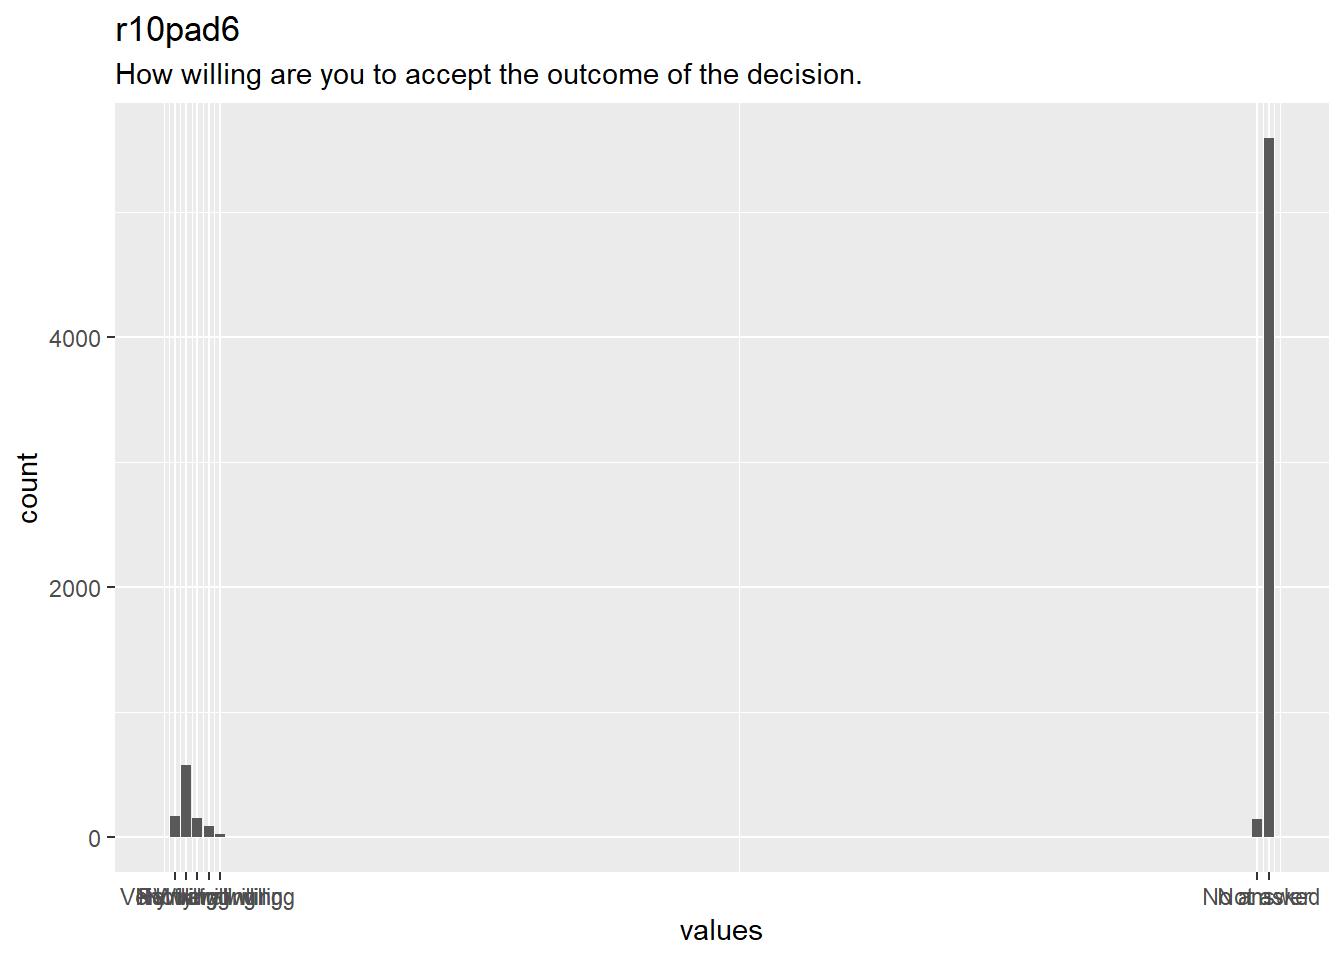
\includegraphics{Goodloser-appendix_files/figure-latex/r10pad6_distribution-1.pdf}

10246 missings.

\subsubsection{Summary statistics}\label{r10pad6_summary}

name

label

data\_type

value\_labels

missing

complete

n

mean

sd

p0

p25

p50

p75

p100

hist

format.spss

r10pad6

How willing are you to accept the outcome of the decision.

numeric

\begin{enumerate}
\def\labelenumi{\arabic{enumi}.}
\tightlist
\item
  Very willing,2. Willing,3. Fairly willing,4. Not very willing,5. Not
  at all willing,97. No answer,98. Not asked

  10246

  6765

  17011

  83.46

  34.34

  1

  98

  98

  98

  98

  ▂▁▁▁▁▁▁▇

  F1.0
\end{enumerate}

\subsubsection{Value labels}\label{r10pad6_labels}

\begin{itemize}
\tightlist
\item
  \textbf{Very willing}: \emph{1}
\item
  \textbf{Willing}: \emph{2}
\item
  \textbf{Fairly willing}: \emph{3}
\item
  \textbf{Not very willing}: \emph{4}
\item
  \textbf{Not at all willing}: \emph{5}
\item
  \textbf{No answer}: \emph{97}
\item
  \textbf{Not asked}: \emph{98}
\end{itemize}

\subsection{r10pad7}\label{r10pad7}

Confidence in the politicians making the decision.

\subsubsection{Distribution}\label{r10pad7_distribution}

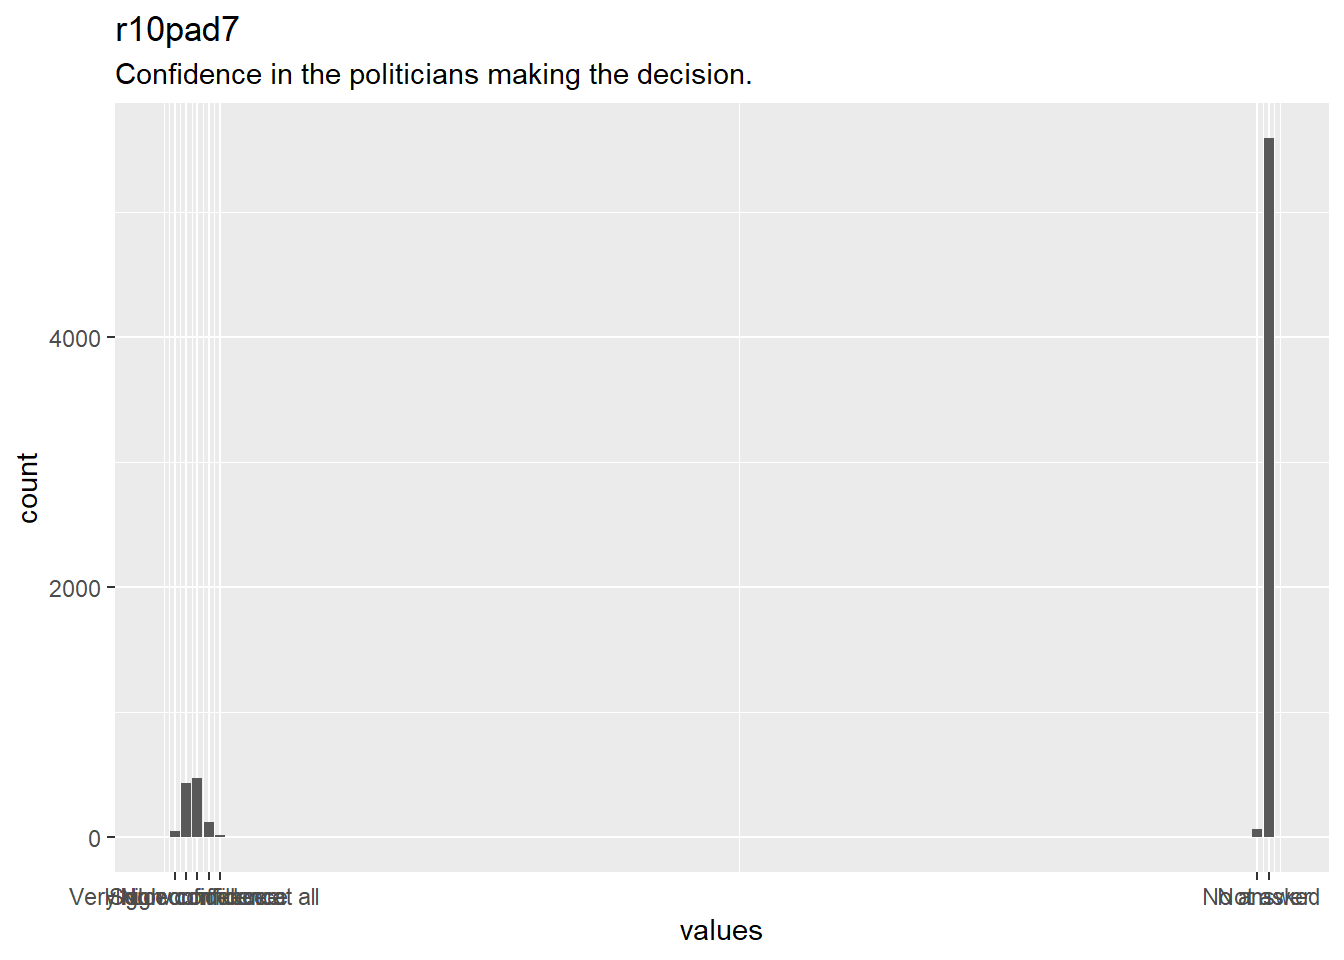
\includegraphics{Goodloser-appendix_files/figure-latex/r10pad7_distribution-1.pdf}

10246 missings.

\subsubsection{Summary statistics}\label{r10pad7_summary}

name

label

data\_type

value\_labels

missing

complete

n

mean

sd

p0

p25

p50

p75

p100

hist

format.spss

r10pad7

Confidence in the politicians making the decision.

numeric

\begin{enumerate}
\def\labelenumi{\arabic{enumi}.}
\tightlist
\item
  Very high confidence,2. High confidence,3. Some confidence,4. Low
  confidence,5. No confidence at all,97. No answer,98. Not asked

  10246

  6765

  17011

  82.44

  35.22

  1

  98

  98

  98

  98

  ▂▁▁▁▁▁▁▇

  F1.0
\end{enumerate}

\subsubsection{Value labels}\label{r10pad7_labels}

\begin{itemize}
\tightlist
\item
  \textbf{Very high confidence}: \emph{1}
\item
  \textbf{High confidence}: \emph{2}
\item
  \textbf{Some confidence}: \emph{3}
\item
  \textbf{Low confidence}: \emph{4}
\item
  \textbf{No confidence at all}: \emph{5}
\item
  \textbf{No answer}: \emph{97}
\item
  \textbf{Not asked}: \emph{98}
\end{itemize}

\subsection{r10pad8}\label{r10pad8}

Outcome in video in line with own view on municipal begging ban.

\subsubsection{Distribution}\label{r10pad8_distribution}

\includegraphics{Goodloser-appendix_files/figure-latex/r10pad8_distribution-1.pdf}

10246 missings.

\subsubsection{Summary statistics}\label{r10pad8_summary}

name

label

data\_type

value\_labels

missing

complete

n

mean

sd

p0

p25

p50

p75

p100

hist

format.spss

r10pad8

Outcome in video in line with own view on municipal begging ban.

numeric

\begin{enumerate}
\def\labelenumi{\arabic{enumi}.}
\tightlist
\item
  Yes,2. No,3. Don't remember,4. Don't know,97. No answer,98. Not asked

  10246

  6765

  17011

  82.27

  35.56

  1

  98

  98

  98

  98

  ▂▁▁▁▁▁▁▇

  F1.0
\end{enumerate}

\subsubsection{Value labels}\label{r10pad8_labels}

\begin{itemize}
\tightlist
\item
  \textbf{Yes}: \emph{1}
\item
  \textbf{No}: \emph{2}
\item
  \textbf{Don't remember}: \emph{3}
\item
  \textbf{Don't know}: \emph{4}
\item
  \textbf{No answer}: \emph{97}
\item
  \textbf{Not asked}: \emph{98}
\end{itemize}

\subsection{r10pad9}\label{r10pad9}

Picture included at the end of video.

\subsubsection{Distribution}\label{r10pad9_distribution}

\includegraphics{Goodloser-appendix_files/figure-latex/r10pad9_distribution-1.pdf}

10246 missings.

\subsubsection{Summary statistics}\label{r10pad9_summary}

name

label

data\_type

value\_labels

missing

complete

n

mean

sd

p0

p25

p50

p75

p100

hist

format.spss

r10pad9

Picture included at the end of video.

numeric

\begin{enumerate}
\def\labelenumi{\arabic{enumi}.}
\tightlist
\item
  Yes, this image was included in the video,2. No, this image was not
  included in the video,97. No answer,98. Not asked

  10246

  6765

  17011

  82.47

  35.43

  1

  98

  98

  98

  98

  ▂▁▁▁▁▁▁▇

  F1.0
\end{enumerate}

\subsubsection{Value labels}\label{r10pad9_labels}

\begin{itemize}
\tightlist
\item
  \textbf{Yes, this image was included in the video}: \emph{1}
\item
  \textbf{No, this image was not included in the video}: \emph{2}
\item
  \textbf{No answer}: \emph{97}
\item
  \textbf{Not asked}: \emph{98}
\end{itemize}

\subsection{r10pad1\_9\_backward\_1}\label{r10pad1_9_backward_1}

Return button used: R10PAD9 -\textgreater{} R10PAD8

\subsubsection{Distribution}\label{r10pad1_9_backward_1_distribution}

\includegraphics{Goodloser-appendix_files/figure-latex/r10pad1_9_backward_1_distribution-1.pdf}

16875 missings.

\subsubsection{Summary statistics}\label{r10pad1_9_backward_1_summary}

name

label

data\_type

value\_labels

missing

complete

n

mean

sd

p0

p25

p50

p75

p100

hist

format.spss

r10pad1\_9\_backward\_1

Return button used: R10PAD9 -\textgreater{} R10PAD8

numeric

\begin{enumerate}
\def\labelenumi{\arabic{enumi}.}
\tightlist
\item
  Yes, return button used from R10PAD9 -\textgreater{} R10PAD8Â

  16875

  136

  17011

  1

  0

  1

  1

  1

  1

  1

  ▁▁▁▇▁▁▁▁

  F1.0
\end{enumerate}

\subsubsection{Value labels}\label{r10pad1_9_backward_1_labels}

\begin{itemize}
\tightlist
\item
  \textbf{Yes, return button used from R10PAD9 -\textgreater{}
  R10PAD8Â~}: \emph{1}
\end{itemize}

\subsection{r10pad1\_9\_backward\_2}\label{r10pad1_9_backward_2}

Return button used: R10PAD8 -\textgreater{} R10PAD7

\subsubsection{Distribution}\label{r10pad1_9_backward_2_distribution}

\includegraphics{Goodloser-appendix_files/figure-latex/r10pad1_9_backward_2_distribution-1.pdf}

16841 missings.

\subsubsection{Summary statistics}\label{r10pad1_9_backward_2_summary}

name

label

data\_type

value\_labels

missing

complete

n

mean

sd

p0

p25

p50

p75

p100

hist

format.spss

r10pad1\_9\_backward\_2

Return button used: R10PAD8 -\textgreater{} R10PAD7

numeric

\begin{enumerate}
\def\labelenumi{\arabic{enumi}.}
\tightlist
\item
  Yes, return button used from R10PAD8 -\textgreater{} R10PAD7

  16841

  170

  17011

  1

  0

  1

  1

  1

  1

  1

  ▁▁▁▇▁▁▁▁

  F1.0
\end{enumerate}

\subsubsection{Value labels}\label{r10pad1_9_backward_2_labels}

\begin{itemize}
\tightlist
\item
  \textbf{Yes, return button used from R10PAD8 -\textgreater{} R10PAD7}:
  \emph{1}
\end{itemize}

\subsection{r10pad1\_9\_backward\_3}\label{r10pad1_9_backward_3}

Return button used: R10PAD7 -\textgreater{} R10PAD6

\subsubsection{Distribution}\label{r10pad1_9_backward_3_distribution}

\includegraphics{Goodloser-appendix_files/figure-latex/r10pad1_9_backward_3_distribution-1.pdf}

16815 missings.

\subsubsection{Summary statistics}\label{r10pad1_9_backward_3_summary}

name

label

data\_type

value\_labels

missing

complete

n

mean

sd

p0

p25

p50

p75

p100

hist

format.spss

r10pad1\_9\_backward\_3

Return button used: R10PAD7 -\textgreater{} R10PAD6

numeric

\begin{enumerate}
\def\labelenumi{\arabic{enumi}.}
\tightlist
\item
  Yes, return button used from R10PAD7 -\textgreater{} R10PAD6Â

  16815

  196

  17011

  1

  0

  1

  1

  1

  1

  1

  ▁▁▁▇▁▁▁▁

  F1.0
\end{enumerate}

\subsubsection{Value labels}\label{r10pad1_9_backward_3_labels}

\begin{itemize}
\tightlist
\item
  \textbf{Yes, return button used from R10PAD7 -\textgreater{}
  R10PAD6Â~}: \emph{1}
\end{itemize}

\subsection{r10pad1\_9\_backward\_4}\label{r10pad1_9_backward_4}

Return button used: R10PAD6 -\textgreater{} R10PAD5

\subsubsection{Distribution}\label{r10pad1_9_backward_4_distribution}

\includegraphics{Goodloser-appendix_files/figure-latex/r10pad1_9_backward_4_distribution-1.pdf}

16882 missings.

\subsubsection{Summary statistics}\label{r10pad1_9_backward_4_summary}

name

label

data\_type

value\_labels

missing

complete

n

mean

sd

p0

p25

p50

p75

p100

hist

format.spss

r10pad1\_9\_backward\_4

Return button used: R10PAD6 -\textgreater{} R10PAD5

numeric

\begin{enumerate}
\def\labelenumi{\arabic{enumi}.}
\tightlist
\item
  Yes, return button used from R10PAD6 -\textgreater{} R10PAD5

  16882

  129

  17011

  1

  0

  1

  1

  1

  1

  1

  ▁▁▁▇▁▁▁▁

  F1.0
\end{enumerate}

\subsubsection{Value labels}\label{r10pad1_9_backward_4_labels}

\begin{itemize}
\tightlist
\item
  \textbf{Yes, return button used from R10PAD6 -\textgreater{} R10PAD5}:
  \emph{1}
\end{itemize}

\subsection{r10pad1\_9\_backward\_5}\label{r10pad1_9_backward_5}

Return button used: R10PAD5 -\textgreater{} R10PAD4

\subsubsection{Distribution}\label{r10pad1_9_backward_5_distribution}

\includegraphics{Goodloser-appendix_files/figure-latex/r10pad1_9_backward_5_distribution-1.pdf}

16867 missings.

\subsubsection{Summary statistics}\label{r10pad1_9_backward_5_summary}

name

label

data\_type

value\_labels

missing

complete

n

mean

sd

p0

p25

p50

p75

p100

hist

format.spss

r10pad1\_9\_backward\_5

Return button used: R10PAD5 -\textgreater{} R10PAD4

numeric

\begin{enumerate}
\def\labelenumi{\arabic{enumi}.}
\tightlist
\item
  Yes, return button used from R10PAD5 -\textgreater{} R10PAD4

  16867

  144

  17011

  1

  0

  1

  1

  1

  1

  1

  ▁▁▁▇▁▁▁▁

  F1.0
\end{enumerate}

\subsubsection{Value labels}\label{r10pad1_9_backward_5_labels}

\begin{itemize}
\tightlist
\item
  \textbf{Yes, return button used from R10PAD5 -\textgreater{} R10PAD4}:
  \emph{1}
\end{itemize}

\subsection{r10pad1\_9\_backward\_6}\label{r10pad1_9_backward_6}

Return button used: R10PAD4 -\textgreater{} R10PAD3

\subsubsection{Distribution}\label{r10pad1_9_backward_6_distribution}

\includegraphics{Goodloser-appendix_files/figure-latex/r10pad1_9_backward_6_distribution-1.pdf}

16847 missings.

\subsubsection{Summary statistics}\label{r10pad1_9_backward_6_summary}

name

label

data\_type

value\_labels

missing

complete

n

mean

sd

p0

p25

p50

p75

p100

hist

format.spss

r10pad1\_9\_backward\_6

Return button used: R10PAD4 -\textgreater{} R10PAD3

numeric

\begin{enumerate}
\def\labelenumi{\arabic{enumi}.}
\tightlist
\item
  Yes, return button used from R10PAD4 -\textgreater{} R10PAD3

  16847

  164

  17011

  1

  0

  1

  1

  1

  1

  1

  ▁▁▁▇▁▁▁▁

  F1.0
\end{enumerate}

\subsubsection{Value labels}\label{r10pad1_9_backward_6_labels}

\begin{itemize}
\tightlist
\item
  \textbf{Yes, return button used from R10PAD4 -\textgreater{} R10PAD3}:
  \emph{1}
\end{itemize}

\subsection{r10pad1\_9\_backward\_7}\label{r10pad1_9_backward_7}

Return button used: R10PAD3 -\textgreater{} R10PAD2

\subsubsection{Distribution}\label{r10pad1_9_backward_7_distribution}

\includegraphics{Goodloser-appendix_files/figure-latex/r10pad1_9_backward_7_distribution-1.pdf}

16916 missings.

\subsubsection{Summary statistics}\label{r10pad1_9_backward_7_summary}

name

label

data\_type

value\_labels

missing

complete

n

mean

sd

p0

p25

p50

p75

p100

hist

format.spss

r10pad1\_9\_backward\_7

Return button used: R10PAD3 -\textgreater{} R10PAD2

numeric

\begin{enumerate}
\def\labelenumi{\arabic{enumi}.}
\tightlist
\item
  Yes, return button used from R10PAD3 -\textgreater{} R10PAD2Â

  16916

  95

  17011

  1

  0

  1

  1

  1

  1

  1

  ▁▁▁▇▁▁▁▁

  F1.0
\end{enumerate}

\subsubsection{Value labels}\label{r10pad1_9_backward_7_labels}

\begin{itemize}
\tightlist
\item
  \textbf{Yes, return button used from R10PAD3 -\textgreater{}
  R10PAD2Â~}: \emph{1}
\end{itemize}

\subsection{r10pad1\_9\_backward\_8}\label{r10pad1_9_backward_8}

Return button used: R10PAD2 -\textgreater{} R10PAD1

\subsubsection{Distribution}\label{r10pad1_9_backward_8_distribution}

\includegraphics{Goodloser-appendix_files/figure-latex/r10pad1_9_backward_8_distribution-1.pdf}

16932 missings.

\subsubsection{Summary statistics}\label{r10pad1_9_backward_8_summary}

name

label

data\_type

value\_labels

missing

complete

n

mean

sd

p0

p25

p50

p75

p100

hist

format.spss

r10pad1\_9\_backward\_8

Return button used: R10PAD2 -\textgreater{} R10PAD1

numeric

\begin{enumerate}
\def\labelenumi{\arabic{enumi}.}
\tightlist
\item
  Yes, return button used from R10PAD2 -\textgreater{} R10PAD1

  16932

  79

  17011

  1

  0

  1

  1

  1

  1

  1

  ▁▁▁▇▁▁▁▁

  F1.0
\end{enumerate}

\subsubsection{Value labels}\label{r10pad1_9_backward_8_labels}

\begin{itemize}
\tightlist
\item
  \textbf{Yes, return button used from R10PAD2 -\textgreater{} R10PAD1}:
  \emph{1}
\end{itemize}

\section{Missingness report}\label{missingness-report-1}

Among those who finished the survey. Only variables that have missings
are shown.

\begin{longtable}[]{@{}cccccc@{}}
\caption{Table continues below}\tabularnewline
\toprule
\begin{minipage}[b]{0.28\columnwidth}\centering\strut
description\strut
\end{minipage} & \begin{minipage}[b]{0.14\columnwidth}\centering\strut
responseid\strut
\end{minipage} & \begin{minipage}[b]{0.09\columnwidth}\centering\strut
r9pad1\strut
\end{minipage} & \begin{minipage}[b]{0.09\columnwidth}\centering\strut
r9pad2\strut
\end{minipage} & \begin{minipage}[b]{0.09\columnwidth}\centering\strut
r9pad3\strut
\end{minipage} & \begin{minipage}[b]{0.14\columnwidth}\centering\strut
r10panelpad\strut
\end{minipage}\tabularnewline
\midrule
\endfirsthead
\toprule
\begin{minipage}[b]{0.28\columnwidth}\centering\strut
description\strut
\end{minipage} & \begin{minipage}[b]{0.14\columnwidth}\centering\strut
responseid\strut
\end{minipage} & \begin{minipage}[b]{0.09\columnwidth}\centering\strut
r9pad1\strut
\end{minipage} & \begin{minipage}[b]{0.09\columnwidth}\centering\strut
r9pad2\strut
\end{minipage} & \begin{minipage}[b]{0.09\columnwidth}\centering\strut
r9pad3\strut
\end{minipage} & \begin{minipage}[b]{0.14\columnwidth}\centering\strut
r10panelpad\strut
\end{minipage}\tabularnewline
\midrule
\endhead
\begin{minipage}[t]{0.28\columnwidth}\centering\strut
Missings per variable\strut
\end{minipage} & \begin{minipage}[t]{0.14\columnwidth}\centering\strut
1\strut
\end{minipage} & \begin{minipage}[t]{0.09\columnwidth}\centering\strut
10114\strut
\end{minipage} & \begin{minipage}[t]{0.09\columnwidth}\centering\strut
10114\strut
\end{minipage} & \begin{minipage}[t]{0.09\columnwidth}\centering\strut
10114\strut
\end{minipage} & \begin{minipage}[t]{0.14\columnwidth}\centering\strut
10246\strut
\end{minipage}\tabularnewline
\begin{minipage}[t]{0.28\columnwidth}\centering\strut
Missings in 28 variables\strut
\end{minipage} & \begin{minipage}[t]{0.14\columnwidth}\centering\strut
1\strut
\end{minipage} & \begin{minipage}[t]{0.09\columnwidth}\centering\strut
0\strut
\end{minipage} & \begin{minipage}[t]{0.09\columnwidth}\centering\strut
0\strut
\end{minipage} & \begin{minipage}[t]{0.09\columnwidth}\centering\strut
0\strut
\end{minipage} & \begin{minipage}[t]{0.14\columnwidth}\centering\strut
0\strut
\end{minipage}\tabularnewline
\begin{minipage}[t]{0.28\columnwidth}\centering\strut
Missings in 16 variables\strut
\end{minipage} & \begin{minipage}[t]{0.14\columnwidth}\centering\strut
1\strut
\end{minipage} & \begin{minipage}[t]{0.09\columnwidth}\centering\strut
1\strut
\end{minipage} & \begin{minipage}[t]{0.09\columnwidth}\centering\strut
1\strut
\end{minipage} & \begin{minipage}[t]{0.09\columnwidth}\centering\strut
1\strut
\end{minipage} & \begin{minipage}[t]{0.14\columnwidth}\centering\strut
1\strut
\end{minipage}\tabularnewline
\begin{minipage}[t]{0.28\columnwidth}\centering\strut
Missings in 25 variables\strut
\end{minipage} & \begin{minipage}[t]{0.14\columnwidth}\centering\strut
1\strut
\end{minipage} & \begin{minipage}[t]{0.09\columnwidth}\centering\strut
1\strut
\end{minipage} & \begin{minipage}[t]{0.09\columnwidth}\centering\strut
1\strut
\end{minipage} & \begin{minipage}[t]{0.09\columnwidth}\centering\strut
1\strut
\end{minipage} & \begin{minipage}[t]{0.14\columnwidth}\centering\strut
0\strut
\end{minipage}\tabularnewline
\begin{minipage}[t]{0.28\columnwidth}\centering\strut
Missings in 19 variables\strut
\end{minipage} & \begin{minipage}[t]{0.14\columnwidth}\centering\strut
1\strut
\end{minipage} & \begin{minipage}[t]{0.09\columnwidth}\centering\strut
0\strut
\end{minipage} & \begin{minipage}[t]{0.09\columnwidth}\centering\strut
0\strut
\end{minipage} & \begin{minipage}[t]{0.09\columnwidth}\centering\strut
0\strut
\end{minipage} & \begin{minipage}[t]{0.14\columnwidth}\centering\strut
1\strut
\end{minipage}\tabularnewline
\begin{minipage}[t]{0.28\columnwidth}\centering\strut
Missings in 10 variables\strut
\end{minipage} & \begin{minipage}[t]{0.14\columnwidth}\centering\strut
1\strut
\end{minipage} & \begin{minipage}[t]{0.09\columnwidth}\centering\strut
1\strut
\end{minipage} & \begin{minipage}[t]{0.09\columnwidth}\centering\strut
1\strut
\end{minipage} & \begin{minipage}[t]{0.09\columnwidth}\centering\strut
1\strut
\end{minipage} & \begin{minipage}[t]{0.14\columnwidth}\centering\strut
1\strut
\end{minipage}\tabularnewline
\begin{minipage}[t]{0.28\columnwidth}\centering\strut
Missings in 13 variables\strut
\end{minipage} & \begin{minipage}[t]{0.14\columnwidth}\centering\strut
1\strut
\end{minipage} & \begin{minipage}[t]{0.09\columnwidth}\centering\strut
1\strut
\end{minipage} & \begin{minipage}[t]{0.09\columnwidth}\centering\strut
1\strut
\end{minipage} & \begin{minipage}[t]{0.09\columnwidth}\centering\strut
1\strut
\end{minipage} & \begin{minipage}[t]{0.14\columnwidth}\centering\strut
1\strut
\end{minipage}\tabularnewline
\begin{minipage}[t]{0.28\columnwidth}\centering\strut
186 other, less frequent patterns\strut
\end{minipage} & \begin{minipage}[t]{0.14\columnwidth}\centering\strut
185\strut
\end{minipage} & \begin{minipage}[t]{0.09\columnwidth}\centering\strut
168\strut
\end{minipage} & \begin{minipage}[t]{0.09\columnwidth}\centering\strut
168\strut
\end{minipage} & \begin{minipage}[t]{0.09\columnwidth}\centering\strut
168\strut
\end{minipage} & \begin{minipage}[t]{0.14\columnwidth}\centering\strut
185\strut
\end{minipage}\tabularnewline
\bottomrule
\end{longtable}

\begin{longtable}[]{@{}cccccccc@{}}
\caption{Table continues below}\tabularnewline
\toprule
\begin{minipage}[b]{0.10\columnwidth}\centering\strut
r10pad1\strut
\end{minipage} & \begin{minipage}[b]{0.10\columnwidth}\centering\strut
r10pad2\strut
\end{minipage} & \begin{minipage}[b]{0.10\columnwidth}\centering\strut
r10pad4\strut
\end{minipage} & \begin{minipage}[b]{0.10\columnwidth}\centering\strut
r10pad5\strut
\end{minipage} & \begin{minipage}[b]{0.10\columnwidth}\centering\strut
r10pad6\strut
\end{minipage} & \begin{minipage}[b]{0.10\columnwidth}\centering\strut
r10pad7\strut
\end{minipage} & \begin{minipage}[b]{0.10\columnwidth}\centering\strut
r10pad8\strut
\end{minipage} & \begin{minipage}[b]{0.10\columnwidth}\centering\strut
r10pad9\strut
\end{minipage}\tabularnewline
\midrule
\endfirsthead
\toprule
\begin{minipage}[b]{0.10\columnwidth}\centering\strut
r10pad1\strut
\end{minipage} & \begin{minipage}[b]{0.10\columnwidth}\centering\strut
r10pad2\strut
\end{minipage} & \begin{minipage}[b]{0.10\columnwidth}\centering\strut
r10pad4\strut
\end{minipage} & \begin{minipage}[b]{0.10\columnwidth}\centering\strut
r10pad5\strut
\end{minipage} & \begin{minipage}[b]{0.10\columnwidth}\centering\strut
r10pad6\strut
\end{minipage} & \begin{minipage}[b]{0.10\columnwidth}\centering\strut
r10pad7\strut
\end{minipage} & \begin{minipage}[b]{0.10\columnwidth}\centering\strut
r10pad8\strut
\end{minipage} & \begin{minipage}[b]{0.10\columnwidth}\centering\strut
r10pad9\strut
\end{minipage}\tabularnewline
\midrule
\endhead
\begin{minipage}[t]{0.10\columnwidth}\centering\strut
10246\strut
\end{minipage} & \begin{minipage}[t]{0.10\columnwidth}\centering\strut
10246\strut
\end{minipage} & \begin{minipage}[t]{0.10\columnwidth}\centering\strut
10246\strut
\end{minipage} & \begin{minipage}[t]{0.10\columnwidth}\centering\strut
10246\strut
\end{minipage} & \begin{minipage}[t]{0.10\columnwidth}\centering\strut
10246\strut
\end{minipage} & \begin{minipage}[t]{0.10\columnwidth}\centering\strut
10246\strut
\end{minipage} & \begin{minipage}[t]{0.10\columnwidth}\centering\strut
10246\strut
\end{minipage} & \begin{minipage}[t]{0.10\columnwidth}\centering\strut
10246\strut
\end{minipage}\tabularnewline
\begin{minipage}[t]{0.10\columnwidth}\centering\strut
0\strut
\end{minipage} & \begin{minipage}[t]{0.10\columnwidth}\centering\strut
0\strut
\end{minipage} & \begin{minipage}[t]{0.10\columnwidth}\centering\strut
0\strut
\end{minipage} & \begin{minipage}[t]{0.10\columnwidth}\centering\strut
0\strut
\end{minipage} & \begin{minipage}[t]{0.10\columnwidth}\centering\strut
0\strut
\end{minipage} & \begin{minipage}[t]{0.10\columnwidth}\centering\strut
0\strut
\end{minipage} & \begin{minipage}[t]{0.10\columnwidth}\centering\strut
0\strut
\end{minipage} & \begin{minipage}[t]{0.10\columnwidth}\centering\strut
0\strut
\end{minipage}\tabularnewline
\begin{minipage}[t]{0.10\columnwidth}\centering\strut
1\strut
\end{minipage} & \begin{minipage}[t]{0.10\columnwidth}\centering\strut
1\strut
\end{minipage} & \begin{minipage}[t]{0.10\columnwidth}\centering\strut
1\strut
\end{minipage} & \begin{minipage}[t]{0.10\columnwidth}\centering\strut
1\strut
\end{minipage} & \begin{minipage}[t]{0.10\columnwidth}\centering\strut
1\strut
\end{minipage} & \begin{minipage}[t]{0.10\columnwidth}\centering\strut
1\strut
\end{minipage} & \begin{minipage}[t]{0.10\columnwidth}\centering\strut
1\strut
\end{minipage} & \begin{minipage}[t]{0.10\columnwidth}\centering\strut
1\strut
\end{minipage}\tabularnewline
\begin{minipage}[t]{0.10\columnwidth}\centering\strut
0\strut
\end{minipage} & \begin{minipage}[t]{0.10\columnwidth}\centering\strut
0\strut
\end{minipage} & \begin{minipage}[t]{0.10\columnwidth}\centering\strut
0\strut
\end{minipage} & \begin{minipage}[t]{0.10\columnwidth}\centering\strut
0\strut
\end{minipage} & \begin{minipage}[t]{0.10\columnwidth}\centering\strut
0\strut
\end{minipage} & \begin{minipage}[t]{0.10\columnwidth}\centering\strut
0\strut
\end{minipage} & \begin{minipage}[t]{0.10\columnwidth}\centering\strut
0\strut
\end{minipage} & \begin{minipage}[t]{0.10\columnwidth}\centering\strut
0\strut
\end{minipage}\tabularnewline
\begin{minipage}[t]{0.10\columnwidth}\centering\strut
1\strut
\end{minipage} & \begin{minipage}[t]{0.10\columnwidth}\centering\strut
1\strut
\end{minipage} & \begin{minipage}[t]{0.10\columnwidth}\centering\strut
1\strut
\end{minipage} & \begin{minipage}[t]{0.10\columnwidth}\centering\strut
1\strut
\end{minipage} & \begin{minipage}[t]{0.10\columnwidth}\centering\strut
1\strut
\end{minipage} & \begin{minipage}[t]{0.10\columnwidth}\centering\strut
1\strut
\end{minipage} & \begin{minipage}[t]{0.10\columnwidth}\centering\strut
1\strut
\end{minipage} & \begin{minipage}[t]{0.10\columnwidth}\centering\strut
1\strut
\end{minipage}\tabularnewline
\begin{minipage}[t]{0.10\columnwidth}\centering\strut
1\strut
\end{minipage} & \begin{minipage}[t]{0.10\columnwidth}\centering\strut
1\strut
\end{minipage} & \begin{minipage}[t]{0.10\columnwidth}\centering\strut
1\strut
\end{minipage} & \begin{minipage}[t]{0.10\columnwidth}\centering\strut
1\strut
\end{minipage} & \begin{minipage}[t]{0.10\columnwidth}\centering\strut
1\strut
\end{minipage} & \begin{minipage}[t]{0.10\columnwidth}\centering\strut
1\strut
\end{minipage} & \begin{minipage}[t]{0.10\columnwidth}\centering\strut
1\strut
\end{minipage} & \begin{minipage}[t]{0.10\columnwidth}\centering\strut
1\strut
\end{minipage}\tabularnewline
\begin{minipage}[t]{0.10\columnwidth}\centering\strut
1\strut
\end{minipage} & \begin{minipage}[t]{0.10\columnwidth}\centering\strut
1\strut
\end{minipage} & \begin{minipage}[t]{0.10\columnwidth}\centering\strut
1\strut
\end{minipage} & \begin{minipage}[t]{0.10\columnwidth}\centering\strut
1\strut
\end{minipage} & \begin{minipage}[t]{0.10\columnwidth}\centering\strut
1\strut
\end{minipage} & \begin{minipage}[t]{0.10\columnwidth}\centering\strut
1\strut
\end{minipage} & \begin{minipage}[t]{0.10\columnwidth}\centering\strut
1\strut
\end{minipage} & \begin{minipage}[t]{0.10\columnwidth}\centering\strut
1\strut
\end{minipage}\tabularnewline
\begin{minipage}[t]{0.10\columnwidth}\centering\strut
185\strut
\end{minipage} & \begin{minipage}[t]{0.10\columnwidth}\centering\strut
185\strut
\end{minipage} & \begin{minipage}[t]{0.10\columnwidth}\centering\strut
185\strut
\end{minipage} & \begin{minipage}[t]{0.10\columnwidth}\centering\strut
185\strut
\end{minipage} & \begin{minipage}[t]{0.10\columnwidth}\centering\strut
185\strut
\end{minipage} & \begin{minipage}[t]{0.10\columnwidth}\centering\strut
185\strut
\end{minipage} & \begin{minipage}[t]{0.10\columnwidth}\centering\strut
185\strut
\end{minipage} & \begin{minipage}[t]{0.10\columnwidth}\centering\strut
185\strut
\end{minipage}\tabularnewline
\bottomrule
\end{longtable}

\begin{longtable}[]{@{}cccc@{}}
\caption{Table continues below}\tabularnewline
\toprule
\begin{minipage}[b]{0.20\columnwidth}\centering\strut
r10pad3\_mobil\strut
\end{minipage} & \begin{minipage}[b]{0.25\columnwidth}\centering\strut
r10pad3\_timespent\strut
\end{minipage} & \begin{minipage}[b]{0.18\columnwidth}\centering\strut
r10pad3a\_ran\strut
\end{minipage} & \begin{minipage}[b]{0.18\columnwidth}\centering\strut
r10pad3played\strut
\end{minipage}\tabularnewline
\midrule
\endfirsthead
\toprule
\begin{minipage}[b]{0.20\columnwidth}\centering\strut
r10pad3\_mobil\strut
\end{minipage} & \begin{minipage}[b]{0.25\columnwidth}\centering\strut
r10pad3\_timespent\strut
\end{minipage} & \begin{minipage}[b]{0.18\columnwidth}\centering\strut
r10pad3a\_ran\strut
\end{minipage} & \begin{minipage}[b]{0.18\columnwidth}\centering\strut
r10pad3played\strut
\end{minipage}\tabularnewline
\midrule
\endhead
\begin{minipage}[t]{0.20\columnwidth}\centering\strut
15732\strut
\end{minipage} & \begin{minipage}[t]{0.25\columnwidth}\centering\strut
15737\strut
\end{minipage} & \begin{minipage}[t]{0.18\columnwidth}\centering\strut
16158\strut
\end{minipage} & \begin{minipage}[t]{0.18\columnwidth}\centering\strut
16178\strut
\end{minipage}\tabularnewline
\begin{minipage}[t]{0.20\columnwidth}\centering\strut
0\strut
\end{minipage} & \begin{minipage}[t]{0.25\columnwidth}\centering\strut
0\strut
\end{minipage} & \begin{minipage}[t]{0.18\columnwidth}\centering\strut
0\strut
\end{minipage} & \begin{minipage}[t]{0.18\columnwidth}\centering\strut
0\strut
\end{minipage}\tabularnewline
\begin{minipage}[t]{0.20\columnwidth}\centering\strut
0\strut
\end{minipage} & \begin{minipage}[t]{0.25\columnwidth}\centering\strut
0\strut
\end{minipage} & \begin{minipage}[t]{0.18\columnwidth}\centering\strut
0\strut
\end{minipage} & \begin{minipage}[t]{0.18\columnwidth}\centering\strut
0\strut
\end{minipage}\tabularnewline
\begin{minipage}[t]{0.20\columnwidth}\centering\strut
0\strut
\end{minipage} & \begin{minipage}[t]{0.25\columnwidth}\centering\strut
0\strut
\end{minipage} & \begin{minipage}[t]{0.18\columnwidth}\centering\strut
0\strut
\end{minipage} & \begin{minipage}[t]{0.18\columnwidth}\centering\strut
0\strut
\end{minipage}\tabularnewline
\begin{minipage}[t]{0.20\columnwidth}\centering\strut
0\strut
\end{minipage} & \begin{minipage}[t]{0.25\columnwidth}\centering\strut
0\strut
\end{minipage} & \begin{minipage}[t]{0.18\columnwidth}\centering\strut
0\strut
\end{minipage} & \begin{minipage}[t]{0.18\columnwidth}\centering\strut
0\strut
\end{minipage}\tabularnewline
\begin{minipage}[t]{0.20\columnwidth}\centering\strut
1\strut
\end{minipage} & \begin{minipage}[t]{0.25\columnwidth}\centering\strut
1\strut
\end{minipage} & \begin{minipage}[t]{0.18\columnwidth}\centering\strut
1\strut
\end{minipage} & \begin{minipage}[t]{0.18\columnwidth}\centering\strut
1\strut
\end{minipage}\tabularnewline
\begin{minipage}[t]{0.20\columnwidth}\centering\strut
1\strut
\end{minipage} & \begin{minipage}[t]{0.25\columnwidth}\centering\strut
1\strut
\end{minipage} & \begin{minipage}[t]{0.18\columnwidth}\centering\strut
1\strut
\end{minipage} & \begin{minipage}[t]{0.18\columnwidth}\centering\strut
0\strut
\end{minipage}\tabularnewline
\begin{minipage}[t]{0.20\columnwidth}\centering\strut
185\strut
\end{minipage} & \begin{minipage}[t]{0.25\columnwidth}\centering\strut
183\strut
\end{minipage} & \begin{minipage}[t]{0.18\columnwidth}\centering\strut
115\strut
\end{minipage} & \begin{minipage}[t]{0.18\columnwidth}\centering\strut
123\strut
\end{minipage}\tabularnewline
\bottomrule
\end{longtable}

\begin{longtable}[]{@{}cccc@{}}
\caption{Table continues below}\tabularnewline
\toprule
\begin{minipage}[b]{0.18\columnwidth}\centering\strut
r10pad3ended\strut
\end{minipage} & \begin{minipage}[b]{0.20\columnwidth}\centering\strut
r10pad3paused\strut
\end{minipage} & \begin{minipage}[b]{0.18\columnwidth}\centering\strut
r10pad3b\_ran\strut
\end{minipage} & \begin{minipage}[b]{0.27\columnwidth}\centering\strut
r10pad1\_9\_backward\_3\strut
\end{minipage}\tabularnewline
\midrule
\endfirsthead
\toprule
\begin{minipage}[b]{0.18\columnwidth}\centering\strut
r10pad3ended\strut
\end{minipage} & \begin{minipage}[b]{0.20\columnwidth}\centering\strut
r10pad3paused\strut
\end{minipage} & \begin{minipage}[b]{0.18\columnwidth}\centering\strut
r10pad3b\_ran\strut
\end{minipage} & \begin{minipage}[b]{0.27\columnwidth}\centering\strut
r10pad1\_9\_backward\_3\strut
\end{minipage}\tabularnewline
\midrule
\endhead
\begin{minipage}[t]{0.18\columnwidth}\centering\strut
16222\strut
\end{minipage} & \begin{minipage}[t]{0.20\columnwidth}\centering\strut
16318\strut
\end{minipage} & \begin{minipage}[t]{0.18\columnwidth}\centering\strut
16585\strut
\end{minipage} & \begin{minipage}[t]{0.27\columnwidth}\centering\strut
16815\strut
\end{minipage}\tabularnewline
\begin{minipage}[t]{0.18\columnwidth}\centering\strut
0\strut
\end{minipage} & \begin{minipage}[t]{0.20\columnwidth}\centering\strut
0\strut
\end{minipage} & \begin{minipage}[t]{0.18\columnwidth}\centering\strut
0\strut
\end{minipage} & \begin{minipage}[t]{0.27\columnwidth}\centering\strut
0\strut
\end{minipage}\tabularnewline
\begin{minipage}[t]{0.18\columnwidth}\centering\strut
0\strut
\end{minipage} & \begin{minipage}[t]{0.20\columnwidth}\centering\strut
0\strut
\end{minipage} & \begin{minipage}[t]{0.18\columnwidth}\centering\strut
0\strut
\end{minipage} & \begin{minipage}[t]{0.27\columnwidth}\centering\strut
0\strut
\end{minipage}\tabularnewline
\begin{minipage}[t]{0.18\columnwidth}\centering\strut
0\strut
\end{minipage} & \begin{minipage}[t]{0.20\columnwidth}\centering\strut
0\strut
\end{minipage} & \begin{minipage}[t]{0.18\columnwidth}\centering\strut
0\strut
\end{minipage} & \begin{minipage}[t]{0.27\columnwidth}\centering\strut
0\strut
\end{minipage}\tabularnewline
\begin{minipage}[t]{0.18\columnwidth}\centering\strut
0\strut
\end{minipage} & \begin{minipage}[t]{0.20\columnwidth}\centering\strut
0\strut
\end{minipage} & \begin{minipage}[t]{0.18\columnwidth}\centering\strut
0\strut
\end{minipage} & \begin{minipage}[t]{0.27\columnwidth}\centering\strut
0\strut
\end{minipage}\tabularnewline
\begin{minipage}[t]{0.18\columnwidth}\centering\strut
1\strut
\end{minipage} & \begin{minipage}[t]{0.20\columnwidth}\centering\strut
1\strut
\end{minipage} & \begin{minipage}[t]{0.18\columnwidth}\centering\strut
0\strut
\end{minipage} & \begin{minipage}[t]{0.27\columnwidth}\centering\strut
0\strut
\end{minipage}\tabularnewline
\begin{minipage}[t]{0.18\columnwidth}\centering\strut
0\strut
\end{minipage} & \begin{minipage}[t]{0.20\columnwidth}\centering\strut
0\strut
\end{minipage} & \begin{minipage}[t]{0.18\columnwidth}\centering\strut
0\strut
\end{minipage} & \begin{minipage}[t]{0.27\columnwidth}\centering\strut
0\strut
\end{minipage}\tabularnewline
\begin{minipage}[t]{0.18\columnwidth}\centering\strut
111\strut
\end{minipage} & \begin{minipage}[t]{0.20\columnwidth}\centering\strut
88\strut
\end{minipage} & \begin{minipage}[t]{0.18\columnwidth}\centering\strut
70\strut
\end{minipage} & \begin{minipage}[t]{0.27\columnwidth}\centering\strut
77\strut
\end{minipage}\tabularnewline
\bottomrule
\end{longtable}

\begin{longtable}[]{@{}ccc@{}}
\caption{Table continues below}\tabularnewline
\toprule
\begin{minipage}[b]{0.29\columnwidth}\centering\strut
r10pad1\_9\_backward\_2\strut
\end{minipage} & \begin{minipage}[b]{0.29\columnwidth}\centering\strut
r10pad1\_9\_backward\_6\strut
\end{minipage} & \begin{minipage}[b]{0.29\columnwidth}\centering\strut
r10pad1\_9\_backward\_5\strut
\end{minipage}\tabularnewline
\midrule
\endfirsthead
\toprule
\begin{minipage}[b]{0.29\columnwidth}\centering\strut
r10pad1\_9\_backward\_2\strut
\end{minipage} & \begin{minipage}[b]{0.29\columnwidth}\centering\strut
r10pad1\_9\_backward\_6\strut
\end{minipage} & \begin{minipage}[b]{0.29\columnwidth}\centering\strut
r10pad1\_9\_backward\_5\strut
\end{minipage}\tabularnewline
\midrule
\endhead
\begin{minipage}[t]{0.29\columnwidth}\centering\strut
16841\strut
\end{minipage} & \begin{minipage}[t]{0.29\columnwidth}\centering\strut
16847\strut
\end{minipage} & \begin{minipage}[t]{0.29\columnwidth}\centering\strut
16867\strut
\end{minipage}\tabularnewline
\begin{minipage}[t]{0.29\columnwidth}\centering\strut
0\strut
\end{minipage} & \begin{minipage}[t]{0.29\columnwidth}\centering\strut
0\strut
\end{minipage} & \begin{minipage}[t]{0.29\columnwidth}\centering\strut
0\strut
\end{minipage}\tabularnewline
\begin{minipage}[t]{0.29\columnwidth}\centering\strut
0\strut
\end{minipage} & \begin{minipage}[t]{0.29\columnwidth}\centering\strut
0\strut
\end{minipage} & \begin{minipage}[t]{0.29\columnwidth}\centering\strut
0\strut
\end{minipage}\tabularnewline
\begin{minipage}[t]{0.29\columnwidth}\centering\strut
0\strut
\end{minipage} & \begin{minipage}[t]{0.29\columnwidth}\centering\strut
0\strut
\end{minipage} & \begin{minipage}[t]{0.29\columnwidth}\centering\strut
0\strut
\end{minipage}\tabularnewline
\begin{minipage}[t]{0.29\columnwidth}\centering\strut
0\strut
\end{minipage} & \begin{minipage}[t]{0.29\columnwidth}\centering\strut
0\strut
\end{minipage} & \begin{minipage}[t]{0.29\columnwidth}\centering\strut
0\strut
\end{minipage}\tabularnewline
\begin{minipage}[t]{0.29\columnwidth}\centering\strut
0\strut
\end{minipage} & \begin{minipage}[t]{0.29\columnwidth}\centering\strut
0\strut
\end{minipage} & \begin{minipage}[t]{0.29\columnwidth}\centering\strut
0\strut
\end{minipage}\tabularnewline
\begin{minipage}[t]{0.29\columnwidth}\centering\strut
0\strut
\end{minipage} & \begin{minipage}[t]{0.29\columnwidth}\centering\strut
0\strut
\end{minipage} & \begin{minipage}[t]{0.29\columnwidth}\centering\strut
0\strut
\end{minipage}\tabularnewline
\begin{minipage}[t]{0.29\columnwidth}\centering\strut
64\strut
\end{minipage} & \begin{minipage}[t]{0.29\columnwidth}\centering\strut
66\strut
\end{minipage} & \begin{minipage}[t]{0.29\columnwidth}\centering\strut
61\strut
\end{minipage}\tabularnewline
\bottomrule
\end{longtable}

\begin{longtable}[]{@{}ccc@{}}
\caption{Table continues below}\tabularnewline
\toprule
\begin{minipage}[b]{0.29\columnwidth}\centering\strut
r10pad1\_9\_backward\_1\strut
\end{minipage} & \begin{minipage}[b]{0.29\columnwidth}\centering\strut
r10pad1\_9\_backward\_4\strut
\end{minipage} & \begin{minipage}[b]{0.29\columnwidth}\centering\strut
r10pad1\_9\_backward\_7\strut
\end{minipage}\tabularnewline
\midrule
\endfirsthead
\toprule
\begin{minipage}[b]{0.29\columnwidth}\centering\strut
r10pad1\_9\_backward\_1\strut
\end{minipage} & \begin{minipage}[b]{0.29\columnwidth}\centering\strut
r10pad1\_9\_backward\_4\strut
\end{minipage} & \begin{minipage}[b]{0.29\columnwidth}\centering\strut
r10pad1\_9\_backward\_7\strut
\end{minipage}\tabularnewline
\midrule
\endhead
\begin{minipage}[t]{0.29\columnwidth}\centering\strut
16875\strut
\end{minipage} & \begin{minipage}[t]{0.29\columnwidth}\centering\strut
16882\strut
\end{minipage} & \begin{minipage}[t]{0.29\columnwidth}\centering\strut
16916\strut
\end{minipage}\tabularnewline
\begin{minipage}[t]{0.29\columnwidth}\centering\strut
0\strut
\end{minipage} & \begin{minipage}[t]{0.29\columnwidth}\centering\strut
0\strut
\end{minipage} & \begin{minipage}[t]{0.29\columnwidth}\centering\strut
0\strut
\end{minipage}\tabularnewline
\begin{minipage}[t]{0.29\columnwidth}\centering\strut
0\strut
\end{minipage} & \begin{minipage}[t]{0.29\columnwidth}\centering\strut
0\strut
\end{minipage} & \begin{minipage}[t]{0.29\columnwidth}\centering\strut
0\strut
\end{minipage}\tabularnewline
\begin{minipage}[t]{0.29\columnwidth}\centering\strut
0\strut
\end{minipage} & \begin{minipage}[t]{0.29\columnwidth}\centering\strut
0\strut
\end{minipage} & \begin{minipage}[t]{0.29\columnwidth}\centering\strut
0\strut
\end{minipage}\tabularnewline
\begin{minipage}[t]{0.29\columnwidth}\centering\strut
0\strut
\end{minipage} & \begin{minipage}[t]{0.29\columnwidth}\centering\strut
0\strut
\end{minipage} & \begin{minipage}[t]{0.29\columnwidth}\centering\strut
0\strut
\end{minipage}\tabularnewline
\begin{minipage}[t]{0.29\columnwidth}\centering\strut
0\strut
\end{minipage} & \begin{minipage}[t]{0.29\columnwidth}\centering\strut
0\strut
\end{minipage} & \begin{minipage}[t]{0.29\columnwidth}\centering\strut
0\strut
\end{minipage}\tabularnewline
\begin{minipage}[t]{0.29\columnwidth}\centering\strut
0\strut
\end{minipage} & \begin{minipage}[t]{0.29\columnwidth}\centering\strut
0\strut
\end{minipage} & \begin{minipage}[t]{0.29\columnwidth}\centering\strut
0\strut
\end{minipage}\tabularnewline
\begin{minipage}[t]{0.29\columnwidth}\centering\strut
48\strut
\end{minipage} & \begin{minipage}[t]{0.29\columnwidth}\centering\strut
52\strut
\end{minipage} & \begin{minipage}[t]{0.29\columnwidth}\centering\strut
50\strut
\end{minipage}\tabularnewline
\bottomrule
\end{longtable}

\begin{longtable}[]{@{}cccc@{}}
\toprule
\begin{minipage}[b]{0.28\columnwidth}\centering\strut
r10pad1\_9\_backward\_8\strut
\end{minipage} & \begin{minipage}[b]{0.18\columnwidth}\centering\strut
r10pad3error\strut
\end{minipage} & \begin{minipage}[b]{0.14\columnwidth}\centering\strut
var\_miss\strut
\end{minipage} & \begin{minipage}[b]{0.10\columnwidth}\centering\strut
n\_miss\strut
\end{minipage}\tabularnewline
\midrule
\endhead
\begin{minipage}[t]{0.28\columnwidth}\centering\strut
16932\strut
\end{minipage} & \begin{minipage}[t]{0.18\columnwidth}\centering\strut
16992\strut
\end{minipage} & \begin{minipage}[t]{0.14\columnwidth}\centering\strut
387454\strut
\end{minipage} & \begin{minipage}[t]{0.10\columnwidth}\centering\strut
387454\strut
\end{minipage}\tabularnewline
\begin{minipage}[t]{0.28\columnwidth}\centering\strut
0\strut
\end{minipage} & \begin{minipage}[t]{0.18\columnwidth}\centering\strut
0\strut
\end{minipage} & \begin{minipage}[t]{0.14\columnwidth}\centering\strut
28\strut
\end{minipage} & \begin{minipage}[t]{0.10\columnwidth}\centering\strut
8856\strut
\end{minipage}\tabularnewline
\begin{minipage}[t]{0.28\columnwidth}\centering\strut
0\strut
\end{minipage} & \begin{minipage}[t]{0.18\columnwidth}\centering\strut
0\strut
\end{minipage} & \begin{minipage}[t]{0.14\columnwidth}\centering\strut
16\strut
\end{minipage} & \begin{minipage}[t]{0.10\columnwidth}\centering\strut
4260\strut
\end{minipage}\tabularnewline
\begin{minipage}[t]{0.28\columnwidth}\centering\strut
0\strut
\end{minipage} & \begin{minipage}[t]{0.18\columnwidth}\centering\strut
0\strut
\end{minipage} & \begin{minipage}[t]{0.14\columnwidth}\centering\strut
25\strut
\end{minipage} & \begin{minipage}[t]{0.10\columnwidth}\centering\strut
1389\strut
\end{minipage}\tabularnewline
\begin{minipage}[t]{0.28\columnwidth}\centering\strut
0\strut
\end{minipage} & \begin{minipage}[t]{0.18\columnwidth}\centering\strut
0\strut
\end{minipage} & \begin{minipage}[t]{0.14\columnwidth}\centering\strut
19\strut
\end{minipage} & \begin{minipage}[t]{0.10\columnwidth}\centering\strut
1226\strut
\end{minipage}\tabularnewline
\begin{minipage}[t]{0.28\columnwidth}\centering\strut
0\strut
\end{minipage} & \begin{minipage}[t]{0.18\columnwidth}\centering\strut
0\strut
\end{minipage} & \begin{minipage}[t]{0.14\columnwidth}\centering\strut
10\strut
\end{minipage} & \begin{minipage}[t]{0.10\columnwidth}\centering\strut
284\strut
\end{minipage}\tabularnewline
\begin{minipage}[t]{0.28\columnwidth}\centering\strut
0\strut
\end{minipage} & \begin{minipage}[t]{0.18\columnwidth}\centering\strut
0\strut
\end{minipage} & \begin{minipage}[t]{0.14\columnwidth}\centering\strut
13\strut
\end{minipage} & \begin{minipage}[t]{0.10\columnwidth}\centering\strut
183\strut
\end{minipage}\tabularnewline
\begin{minipage}[t]{0.28\columnwidth}\centering\strut
39\strut
\end{minipage} & \begin{minipage}[t]{0.18\columnwidth}\centering\strut
8\strut
\end{minipage} & \begin{minipage}[t]{0.14\columnwidth}\centering\strut
1700\strut
\end{minipage} & \begin{minipage}[t]{0.10\columnwidth}\centering\strut
813\strut
\end{minipage}\tabularnewline
\bottomrule
\end{longtable}

\section{Codebook table}\label{codebook-table-1}

\hypertarget{htmlwidget-15c6157bb50473b6db73}{}

\chapter{Data management}\label{data-management-1}

\begin{quote}
This chapter describes the data management that is conducted prior to
any analysis
\end{quote}

\begin{Shaded}
\begin{Highlighting}[]
\NormalTok{d <-}\StringTok{ }\NormalTok{d }\OperatorTok
\StringTok{  }\KeywordTok{rename}\NormalTok{(}\StringTok{"imp_accept"}\NormalTok{=}\StringTok{ "r9pad1"}\NormalTok{,}
          \StringTok{"other_accept"}\NormalTok{ =}\StringTok{ "r9pad2"}\NormalTok{,}
          \StringTok{"self_accept"}\NormalTok{ =}\StringTok{ "r9pad3"}\NormalTok{,}
          \StringTok{"opinion_ban"}\NormalTok{ =}\StringTok{ "r10pad1"}\NormalTok{,}
          \StringTok{"opinion_strength"}\NormalTok{ =}\StringTok{ "r10pad2"}\NormalTok{,}
          \StringTok{"video_mobile"}\NormalTok{ =}\StringTok{ "r10pad3_mobil"}\NormalTok{,}
          \StringTok{"video_proban_treat"}\NormalTok{ =}\StringTok{ "r10pad3a_ran"}\NormalTok{,}
          \StringTok{"video_antiban_treat"}\NormalTok{ =}\StringTok{ "r10pad3b_ran"}\NormalTok{,}
          \StringTok{"video_ended"}\NormalTok{ =}\StringTok{ "r10pad3ended"}\NormalTok{,}
          \StringTok{"video_error"}\NormalTok{ =}\StringTok{ "r10pad3error"}\NormalTok{,}
          \StringTok{"video_paused"}\NormalTok{ =}\StringTok{ "r10pad3paused"}\NormalTok{,}
          \StringTok{"video_played"}\NormalTok{ =}\StringTok{ "r10pad3played"}\NormalTok{,}
          \StringTok{"video_timespent"}\NormalTok{ =}\StringTok{ "r10pad3_timespent"}\NormalTok{,}
          \StringTok{"video_report"}\NormalTok{ =}\StringTok{ "r10pad4"}\NormalTok{,}
          \StringTok{"fairness"}\NormalTok{ =}\StringTok{ "r10pad5"}\NormalTok{,}
          \StringTok{"accept"}\NormalTok{ =}\StringTok{ "r10pad6"}\NormalTok{,}
          \StringTok{"trust"}\NormalTok{ =}\StringTok{ "r10pad7"}\NormalTok{,}
          \StringTok{"check_outcome"}\NormalTok{ =}\StringTok{ "r10pad8"}\NormalTok{,}
          \StringTok{"check_politician"}\NormalTok{ =}\StringTok{ "r10pad9"}
\NormalTok{  )}

\CommentTok{#Merge treatments with ban and no ban outcomes          }
\NormalTok{d <-}\StringTok{ }\NormalTok{d }\OperatorTok
\StringTok{  }\KeywordTok{gather}\NormalTok{(video, treatment, video_proban_treat}\OperatorTok{:}\NormalTok{video_antiban_treat)}

\CommentTok{#Make NA the respondents with values 98 (Not asked) or 97 (No answer) for entire dataset. (Checked with command 'sum(is.na(Loser$video_timespent)) that no values on that }
\CommentTok{#variable has value 97 or 98)}
\NormalTok{d[d }\OperatorTok{==}\StringTok{ }\DecValTok{97}\NormalTok{] <-}\StringTok{ }\OtherTok{NA}
\NormalTok{d[d }\OperatorTok{==}\StringTok{ }\DecValTok{98}\NormalTok{] <-}\StringTok{ }\OtherTok{NA}

\CommentTok{#Reverse scales}
\NormalTok{d <-}\StringTok{ }\NormalTok{d }\OperatorTok
\StringTok{  }\KeywordTok{mutate}\NormalTok{(}\DataTypeTok{imp_accept =} \OperatorTok{-}\NormalTok{(imp_accept)}\OperatorTok{+}\DecValTok{6}\NormalTok{,}
         \DataTypeTok{other_accept =} \OperatorTok{-}\NormalTok{(other_accept)}\OperatorTok{+}\DecValTok{6}\NormalTok{,}
         \DataTypeTok{self_accept =} \OperatorTok{-}\NormalTok{(self_accept)}\OperatorTok{+}\DecValTok{6}\NormalTok{,}
         \DataTypeTok{opinion_strength =} \OperatorTok{-}\NormalTok{(opinion_strength)}\OperatorTok{+}\DecValTok{6}\NormalTok{,}
         \DataTypeTok{fairness =} \OperatorTok{-}\NormalTok{(fairness)}\OperatorTok{+}\DecValTok{6}\NormalTok{,}
         \DataTypeTok{accept =} \OperatorTok{-}\NormalTok{(accept)}\OperatorTok{+}\DecValTok{6}\NormalTok{,}
         \DataTypeTok{trust =} \OperatorTok{-}\NormalTok{(trust)}\OperatorTok{+}\DecValTok{6}
\NormalTok{  )}


\CommentTok{#Remove respondents who did not see the video properly. Will be used as main data set}
\NormalTok{d <-}\StringTok{ }\NormalTok{d }\OperatorTok
\StringTok{  }\KeywordTok{filter}\NormalTok{(}\OperatorTok{!}\KeywordTok{is.na}\NormalTok{(treatment))}\OperatorTok\StringTok{ }\CommentTok{#Keep all who where assigned to a video treatment}
\StringTok{  }\KeywordTok{filter}\NormalTok{(video_timespent }\OperatorTok\StringTok{ }\DecValTok{60}\OperatorTok{:}\DecValTok{300}\NormalTok{) }\OperatorTok\StringTok{ }\CommentTok{#Keep only those who stayed with the video for more than 60 seconds and less than 300 seconds}
\StringTok{  }\KeywordTok{filter}\NormalTok{(video_report }\OperatorTok\StringTok{ }\KeywordTok{c}\NormalTok{(}\DecValTok{1}\NormalTok{, }\DecValTok{3}\NormalTok{)) }\CommentTok{#Keep only those who reported that they had sound and picture or picture but no sound}

\NormalTok{##Create manipulation check variable that measures whether the respondents correctly identify whether the outcome was favorable or unfavorable to them}
\NormalTok{d <-}\StringTok{ }\NormalTok{d }\OperatorTok
\StringTok{  }\KeywordTok{mutate}\NormalTok{(}\DataTypeTok{favorability =} \KeywordTok{case_when}\NormalTok{(}
\NormalTok{    treatment }\OperatorTok\StringTok{ }\DecValTok{1}\OperatorTok{:}\DecValTok{4} \OperatorTok{~}\StringTok{ "Unfavorable"}\NormalTok{,}
\NormalTok{    treatment }\OperatorTok{==}\StringTok{ }\DecValTok{5}    \OperatorTok{~}\StringTok{ "Favorable"}
\NormalTok{  )}
\NormalTok{  )}\OperatorTok
\StringTok{  }\KeywordTok{mutate}\NormalTok{(}\DataTypeTok{mcheck_favorability =} \KeywordTok{case_when}\NormalTok{(}
    \KeywordTok{is.na}\NormalTok{(favorability) }\OperatorTok{~}\StringTok{ "Incorrect"}\NormalTok{,}
\NormalTok{    favorability}\OperatorTok{==}\StringTok{"Favorable"} \OperatorTok{&}\StringTok{ }\NormalTok{check_outcome}\OperatorTok{==}\DecValTok{1} \OperatorTok{~}\StringTok{ "Correct"}\NormalTok{,}
\NormalTok{    favorability}\OperatorTok{==}\StringTok{"Unfavorable"} \OperatorTok{&}\StringTok{ }\NormalTok{check_outcome}\OperatorTok{==}\DecValTok{2} \OperatorTok{~}\StringTok{ "Correct"}\NormalTok{,}
\NormalTok{    favorability }\OperatorTok\StringTok{ }\DecValTok{3}\OperatorTok{:}\DecValTok{4} \OperatorTok{~}\StringTok{ "Incorrect"}\NormalTok{,}
\NormalTok{    favorability}\OperatorTok{==}\StringTok{"Favorable"} \OperatorTok{&}\StringTok{ }\NormalTok{check_outcome}\OperatorTok{==}\DecValTok{2} \OperatorTok{~}\StringTok{ "Incorrect"}\NormalTok{,}
\NormalTok{    favorability}\OperatorTok{==}\StringTok{"Unfavorable"} \OperatorTok{&}\StringTok{ }\NormalTok{check_outcome}\OperatorTok{==}\DecValTok{1} \OperatorTok{~}\StringTok{ "Incorrect"}
\NormalTok{  )}
\NormalTok{  ) }

\CommentTok{#Label values on treatment variable}
\NormalTok{d <-}\StringTok{ }\NormalTok{d }\OperatorTok
\StringTok{  }\KeywordTok{mutate}\NormalTok{(}\DataTypeTok{treatment =} \KeywordTok{case_when}\NormalTok{(}
\NormalTok{    .[[}\StringTok{"treatment"}\NormalTok{]] }\OperatorTok{==}\StringTok{ }\DecValTok{1} \OperatorTok{~}\StringTok{ "Lamenting politician"}\NormalTok{,}
\NormalTok{    .[[}\StringTok{"treatment"}\NormalTok{]] }\OperatorTok{==}\StringTok{ }\DecValTok{2} \OperatorTok{~}\StringTok{ "Specific prime"}\NormalTok{,}
\NormalTok{    .[[}\StringTok{"treatment"}\NormalTok{]] }\OperatorTok{==}\StringTok{ }\DecValTok{3} \OperatorTok{~}\StringTok{ "General Prime"}\NormalTok{,}
\NormalTok{    .[[}\StringTok{"treatment"}\NormalTok{]] }\OperatorTok{==}\StringTok{ }\DecValTok{4} \OperatorTok{~}\StringTok{ "Not shown"}\NormalTok{,}
\NormalTok{    .[[}\StringTok{"treatment"}\NormalTok{]] }\OperatorTok{==}\StringTok{ }\DecValTok{5} \OperatorTok{~}\StringTok{ "Winner"}\NormalTok{),}
    \DataTypeTok{opinion_ban =} \KeywordTok{case_when}\NormalTok{(}
\NormalTok{    .[[}\StringTok{"opinion_ban"}\NormalTok{]] }\OperatorTok{==}\StringTok{ }\DecValTok{1} \OperatorTok{~}\StringTok{ "Pro"}\NormalTok{,}
\NormalTok{    .[[}\StringTok{"opinion_ban"}\NormalTok{]] }\OperatorTok{==}\StringTok{ }\DecValTok{2} \OperatorTok{~}\StringTok{ "Anti"}\NormalTok{),}
    \DataTypeTok{responseid =} \KeywordTok{as.numeric}\NormalTok{(responseid),}
         \DataTypeTok{imp_accept =} \KeywordTok{case_when}\NormalTok{(imp_accept }\OperatorTok\StringTok{ }\DecValTok{4}\OperatorTok{:}\DecValTok{5} \OperatorTok{~}\StringTok{ "Important"}\NormalTok{,}
\NormalTok{                                imp_accept }\OperatorTok\StringTok{ }\DecValTok{1}\OperatorTok{:}\DecValTok{3} \OperatorTok{~}\StringTok{ "Not important"}\NormalTok{),}
         \DataTypeTok{other_accept =} \KeywordTok{case_when}\NormalTok{(other_accept }\OperatorTok\StringTok{ }\DecValTok{4}\OperatorTok{:}\DecValTok{5} \OperatorTok{~}\StringTok{ "High degree"}\NormalTok{,}
\NormalTok{                                  other_accept }\OperatorTok\StringTok{ }\DecValTok{1}\OperatorTok{:}\DecValTok{3} \OperatorTok{~}\StringTok{ "Low degree"}\NormalTok{),}
         \DataTypeTok{self_accept =} \KeywordTok{case_when}\NormalTok{(self_accept }\OperatorTok\StringTok{ }\DecValTok{4}\OperatorTok{:}\DecValTok{5} \OperatorTok{~}\StringTok{ "High degree"}\NormalTok{,}
\NormalTok{                                 self_accept }\OperatorTok\StringTok{ }\DecValTok{1}\OperatorTok{:}\DecValTok{3} \OperatorTok{~}\StringTok{ "Low degree"}\NormalTok{),}
         \DataTypeTok{opinion_strength =} \KeywordTok{case_when}\NormalTok{(opinion_strength }\OperatorTok\StringTok{ }\DecValTok{4}\OperatorTok{:}\DecValTok{5} \OperatorTok{~}\StringTok{ "Important"}\NormalTok{,}
\NormalTok{                                      opinion_strength }\OperatorTok\StringTok{ }\DecValTok{1}\OperatorTok{:}\DecValTok{3} \OperatorTok{~}\StringTok{ "Not important"}\NormalTok{)}
\NormalTok{  )}
\CommentTok{#Save file with the main data set}
\KeywordTok{write_sav}\NormalTok{(d, }\StringTok{"Data/Goodloser-exp2.sav"}\NormalTok{)}
\KeywordTok{write_csv}\NormalTok{(d, }\StringTok{"Data/Goodloser-exp2.csv"}\NormalTok{)}

\CommentTok{#----------------------------------------------------}
\CommentTok{#Prepare redux data set, where respondents who fail the manipulation check are excluded}
\CommentTok{#----------------------------------------------------}

\CommentTok{#Create a separate data set where also those who fail the manipulation check are excluded.}
\NormalTok{Loser_redux <-}\StringTok{ }\NormalTok{d }\OperatorTok
\StringTok{  }\KeywordTok{filter}\NormalTok{(mcheck_favorability }\OperatorTok{==}\StringTok{ "Correct"}\NormalTok{)}

\CommentTok{#Save file with the redux good loser data set}

\KeywordTok{write_sav}\NormalTok{(Loser_redux, }\StringTok{"Loser_redux.sav"}\NormalTok{)}
\KeywordTok{write_csv}\NormalTok{(Loser_redux, }\StringTok{"Loser_redux.csv"}\NormalTok{)}


\CommentTok{#d <- d %>%}
\CommentTok{#  mutate(treatment = case_when(}
\CommentTok{#    .[["treatment"]] == 1 ~ "minority spokesperson disappointed and against the outcome",}
\CommentTok{#    .[["treatment"]] == 2 ~ "minority spokesperson disappointed and against the outcome, but procedure was fair so outcome must be accepted",}
\CommentTok{#    .[["treatment"]] == 3 ~ "minority spokesperson disappointed and against the outcome, but losses must be accepted in a democracy",}
\CommentTok{#    .[["treatment"]] == 4 ~ "control - no additional information",}
\CommentTok{#    .[["treatment"]] == 5 ~ "winner control - no additional information")}
\CommentTok{#  )}
\end{Highlighting}
\end{Shaded}

\chapter{Main effects}\label{main-effects-1}

\begin{quote}
This chapter explores the first hypothesis in the
\href{GoogLoser_Prereg_3_\#16823\%5B16065\%5D.pdf}{pre-registration} of
the experiment: \textbf{Individuals that receive an unfavorable outcome
express lower fairness perception than individuals that receive a
favorable outcome.} The estimation of the Average Marginal Component
Effects is based on the function developed by Mikael P. Johannesson, and
available on
\href{https://rdrr.io/github/mikajoh/descr2/man/amce.html}{Github}.
\end{quote}

\begin{Shaded}
\begin{Highlighting}[]
\ControlFlowTok{if}\NormalTok{(}\OperatorTok{!}\KeywordTok{require}\NormalTok{(}\StringTok{"broom"}\NormalTok{))\{}\KeywordTok{install.packages}\NormalTok{(}\StringTok{"broom"}\NormalTok{);  }\KeywordTok{library}\NormalTok{(broom)\}}
\ControlFlowTok{if}\NormalTok{(}\OperatorTok{!}\KeywordTok{require}\NormalTok{(}\StringTok{"haven"}\NormalTok{))\{}\KeywordTok{install.packages}\NormalTok{(}\StringTok{"haven"}\NormalTok{);  }\KeywordTok{library}\NormalTok{(haven)\}}
\ControlFlowTok{if}\NormalTok{(}\OperatorTok{!}\KeywordTok{require}\NormalTok{(}\StringTok{"here"}\NormalTok{))\{}\KeywordTok{install.packages}\NormalTok{(}\StringTok{"here"}\NormalTok{);  }\KeywordTok{library}\NormalTok{(here)\}}
\ControlFlowTok{if}\NormalTok{(}\OperatorTok{!}\KeywordTok{require}\NormalTok{(}\StringTok{"knitr"}\NormalTok{))\{}\KeywordTok{install.packages}\NormalTok{(}\StringTok{"knitr"}\NormalTok{);  }\KeywordTok{library}\NormalTok{(knitr)\}}
\KeywordTok{options}\NormalTok{(}\DataTypeTok{kableExtra.latex.load_packages =} \OtherTok{FALSE}\NormalTok{) }
\ControlFlowTok{if}\NormalTok{(}\OperatorTok{!}\KeywordTok{require}\NormalTok{(}\StringTok{"kableExtra"}\NormalTok{))\{}\KeywordTok{install.packages}\NormalTok{(}\StringTok{"kableExtra"}\NormalTok{);  }\KeywordTok{library}\NormalTok{(kableExtra)\}}
\ControlFlowTok{if}\NormalTok{(}\OperatorTok{!}\KeywordTok{require}\NormalTok{(}\StringTok{"naniar"}\NormalTok{))\{}\KeywordTok{install.packages}\NormalTok{(}\StringTok{"naniar"}\NormalTok{);  }\KeywordTok{library}\NormalTok{(naniar)\}}
\ControlFlowTok{if}\NormalTok{(}\OperatorTok{!}\KeywordTok{require}\NormalTok{(}\StringTok{"tidyverse"}\NormalTok{))\{}\KeywordTok{install.packages}\NormalTok{(}\StringTok{"tidyverse"}\NormalTok{);  }\KeywordTok{library}\NormalTok{(tidyverse)\}}
\CommentTok{# The analysis uses custom functions included in the compendium. Install the included pkg with `devtools::install()` or just install from github with:}
\ControlFlowTok{if}\NormalTok{ (}\OperatorTok{!}\KeywordTok{require}\NormalTok{(wiggle)) \{  devtools}\OperatorTok{::}\KeywordTok{install_github}\NormalTok{(}\StringTok{"mikajoh/wiggle"}\NormalTok{)\}}

\KeywordTok{set.seed}\NormalTok{(}\DecValTok{2016}\NormalTok{)}
\NormalTok{## Utils. }
\KeywordTok{source}\NormalTok{(}\StringTok{"goodloser-utils.R"}\NormalTok{)}

\NormalTok{d <-}\StringTok{ }\KeywordTok{read_sav}\NormalTok{(}\StringTok{"Data/Goodloser-exp2.sav"}\NormalTok{)}

\NormalTok{knitr}\OperatorTok{::}\NormalTok{opts_chunk}\OperatorTok{$}\KeywordTok{set}\NormalTok{(}\DataTypeTok{echo =} \OtherTok{TRUE}\NormalTok{, }\DataTypeTok{knitr.kable.NA =} \StringTok{""}\NormalTok{, }\DataTypeTok{cache =} \OtherTok{FALSE}\NormalTok{, }\DataTypeTok{warning =} \OtherTok{FALSE}\NormalTok{)}
\end{Highlighting}
\end{Shaded}

\section{Prepare data}\label{prepare-data-3}

\begin{Shaded}
\begin{Highlighting}[]
\NormalTok{d <-}\StringTok{ }\NormalTok{d }\OperatorTok
\StringTok{  }\KeywordTok{mutate}\NormalTok{(}\DataTypeTok{treatment =} \KeywordTok{lvls_reorder}\NormalTok{(treatment, }\KeywordTok{c}\NormalTok{(}\DecValTok{3}\NormalTok{, }\DecValTok{2}\NormalTok{, }\DecValTok{1}\NormalTok{, }\DecValTok{4}\NormalTok{, }\DecValTok{5}\NormalTok{)) }
\NormalTok{  )}
\end{Highlighting}
\end{Shaded}

\section{Fairness}\label{fairness-3}

\begin{Shaded}
\begin{Highlighting}[]
\NormalTok{res_main <-}\StringTok{  }\KeywordTok{lm}\NormalTok{(fairness }\OperatorTok{~}\StringTok{ }\NormalTok{treatment, }\DataTypeTok{data =}\NormalTok{ d) }
\NormalTok{res_main <-}\StringTok{ }\NormalTok{broom}\OperatorTok{::}\KeywordTok{tidy}\NormalTok{(res_main)}

\NormalTok{labels <-}\StringTok{ }\KeywordTok{data.frame}\NormalTok{(}
  \DataTypeTok{term =} \KeywordTok{c}\NormalTok{(}
    \StringTok{"treatmentLamenting politician"}\NormalTok{,}
    \StringTok{"treatmentGeneral Prime"}\NormalTok{,}
    \StringTok{"treatmentSpecific prime"}\NormalTok{,}
    \StringTok{"treatmentWinner"}
    
\NormalTok{  ),}
  \DataTypeTok{label =} \KeywordTok{c}\NormalTok{( }\StringTok{"Lamenting politician"}\NormalTok{,}
             \StringTok{"General prime"}\NormalTok{,}
             \StringTok{"Specific prime"}\NormalTok{,}
             \StringTok{"Winner"}\NormalTok{)}
\NormalTok{)}
\CommentTok{#Figure}
\NormalTok{fig <-}\StringTok{   }\NormalTok{res_main }\OperatorTok
\StringTok{  }\KeywordTok{filter}\NormalTok{(term }\OperatorTok{!=}\StringTok{ "(Intercept)"}\NormalTok{) }\OperatorTok\StringTok{ }
\StringTok{  }\KeywordTok{left_join}\NormalTok{(labels, }\DataTypeTok{by =} \StringTok{"term"}\NormalTok{) }\OperatorTok\StringTok{ }
\StringTok{  }
\StringTok{  }\KeywordTok{ggplot}\NormalTok{(}\KeywordTok{aes}\NormalTok{(}\DataTypeTok{x =}\NormalTok{ estimate, }\DataTypeTok{y =}\NormalTok{ label,}
             \DataTypeTok{xmin =}\NormalTok{ estimate }\OperatorTok{-}\StringTok{ }\NormalTok{(}\DecValTok{2} \OperatorTok{*}\StringTok{ }\NormalTok{std.error),}
             \DataTypeTok{xmax =}\NormalTok{ estimate }\OperatorTok{+}\StringTok{ }\NormalTok{(}\DecValTok{2} \OperatorTok{*}\StringTok{ }\NormalTok{std.error))) }\OperatorTok{+}
\StringTok{   }\KeywordTok{geom_errorbarh}\NormalTok{(}\DataTypeTok{height =} \DecValTok{0}\NormalTok{) }\OperatorTok{+}
\StringTok{  }\KeywordTok{geom_point}\NormalTok{() }\OperatorTok{+}
\StringTok{  }\KeywordTok{geom_vline}\NormalTok{(}\KeywordTok{aes}\NormalTok{(}\DataTypeTok{xintercept =} \DecValTok{0}\NormalTok{), }\DataTypeTok{linetype =} \StringTok{"dotted"}\NormalTok{) }\OperatorTok{+}
\StringTok{  }\KeywordTok{scale_x_continuous}\NormalTok{(}\DataTypeTok{limits =} \KeywordTok{c}\NormalTok{(}\OperatorTok{-}\DecValTok{1}\NormalTok{, }\DecValTok{1}\NormalTok{),}
                     \DataTypeTok{breaks =} \KeywordTok{round}\NormalTok{(}\KeywordTok{seq}\NormalTok{(}\OperatorTok{-}\DecValTok{1}\NormalTok{, }\DecValTok{1}\NormalTok{, .}\DecValTok{25}\NormalTok{), }\DecValTok{2}\NormalTok{),}
                     \DataTypeTok{expand =} \KeywordTok{c}\NormalTok{(}\DecValTok{0}\NormalTok{, }\DecValTok{0}\NormalTok{)) }\OperatorTok{+}
\StringTok{  }\KeywordTok{labs}\NormalTok{(}\DataTypeTok{x =} \StringTok{"Change in fairness perception"}\NormalTok{,}
       \DataTypeTok{y =} \StringTok{"Decision process attributes"}\NormalTok{) }\OperatorTok{+}
\StringTok{  }\KeywordTok{theme_bw}\NormalTok{() }\OperatorTok{+}
\StringTok{  }\KeywordTok{theme}\NormalTok{(}\DataTypeTok{plot.margin =} \KeywordTok{unit}\NormalTok{(}\KeywordTok{c}\NormalTok{(}\DecValTok{2}\NormalTok{, }\DecValTok{2}\NormalTok{, }\DecValTok{2}\NormalTok{, }\DecValTok{2}\NormalTok{), }\StringTok{"mm"}\NormalTok{), }\DataTypeTok{axis.text.x=}\KeywordTok{element_text}\NormalTok{(}\DataTypeTok{size=}\KeywordTok{rel}\NormalTok{(}\FloatTok{0.7}\NormalTok{))) }\OperatorTok{+}
\StringTok{  }\KeywordTok{theme}\NormalTok{(}\DataTypeTok{panel.spacing =} \KeywordTok{unit}\NormalTok{(}\FloatTok{0.5}\NormalTok{, }\StringTok{"lines"}\NormalTok{))}
\NormalTok{fig}
\end{Highlighting}
\end{Shaded}

\includegraphics{Goodloser-appendix_files/figure-latex/204_post_fairness-1.pdf}

\begin{Shaded}
\begin{Highlighting}[]
\KeywordTok{ggsave}\NormalTok{(}
  \KeywordTok{here}\NormalTok{(}\StringTok{"output"}\NormalTok{, }\StringTok{"novig"}\NormalTok{, }\StringTok{"figs"}\NormalTok{, }\StringTok{"pngs"}\NormalTok{, }\StringTok{"exp2-fairness-mainfig.png"}\NormalTok{),}
  \DataTypeTok{plot =}\NormalTok{ fig,}
  \DataTypeTok{width =} \FloatTok{5.5}\NormalTok{, }\DataTypeTok{height =} \FloatTok{2.75}
\NormalTok{)}

\KeywordTok{ggsave}\NormalTok{(}
  \KeywordTok{here}\NormalTok{(}\StringTok{"output"}\NormalTok{, }\StringTok{"novig"}\NormalTok{, }\StringTok{"figs"}\NormalTok{, }\StringTok{"pdfs"}\NormalTok{, }\StringTok{"exp2-fairness-mainfig.pdf"}\NormalTok{),}
  \DataTypeTok{plot =}\NormalTok{ fig,}
  \DataTypeTok{width =} \FloatTok{5.5}\NormalTok{, }\DataTypeTok{height =} \FloatTok{2.75}
\NormalTok{)}


\CommentTok{#Table}
\NormalTok{table <-}\StringTok{ }\NormalTok{res_main }\OperatorTok\StringTok{ }
\StringTok{  }\KeywordTok{select}\NormalTok{(term, estimate, std.error, statistic, p.value) }\OperatorTok\StringTok{ }
\StringTok{  }\KeywordTok{mutate}\NormalTok{(}\DataTypeTok{term =} \KeywordTok{case_when}\NormalTok{( term }\OperatorTok{==}\StringTok{ "(Intercept)"} \OperatorTok{~}\StringTok{ "Not shown"}\NormalTok{,}
\NormalTok{                    term }\OperatorTok{==}\StringTok{ "treatmentLamenting politician"} \OperatorTok{~}\StringTok{ "Lamenting politician"}\NormalTok{,}
\NormalTok{                   term }\OperatorTok{==}\StringTok{ "treatmentGeneral Prime"} \OperatorTok{~}\StringTok{ "General prime"}\NormalTok{, }
\NormalTok{                   term }\OperatorTok{==}\StringTok{ "treatmentSpecific prime"} \OperatorTok{~}\StringTok{ "Specific prime"}\NormalTok{,}
\NormalTok{                   term }\OperatorTok{==}\StringTok{ "treatmentWinner"} \OperatorTok{~}\StringTok{ "Winner"}\NormalTok{))}

\KeywordTok{kable}\NormalTok{(table, }\DataTypeTok{booktabs =} \OtherTok{TRUE}\NormalTok{, }\DataTypeTok{caption =} \StringTok{"Treatment effects on fairness perceptions of decision, Study 2 -- Norwegian vignette"}\NormalTok{, }\DataTypeTok{col.names =} \KeywordTok{linebreak}\NormalTok{(}\KeywordTok{c}\NormalTok{(}\StringTok{"Treatment value"}\NormalTok{, }\StringTok{"Estimate"}\NormalTok{, }\StringTok{"Std. Error"}\NormalTok{, }\StringTok{"t-statistic"}\NormalTok{, }\StringTok{"p value"}\NormalTok{))) }\OperatorTok\StringTok{ }
\StringTok{  }\KeywordTok{kable_styling}\NormalTok{(}\DataTypeTok{bootstrap_options =} \KeywordTok{c}\NormalTok{(}\StringTok{"striped"}\NormalTok{, }\StringTok{"hover"}\NormalTok{, }\StringTok{"responsive"}\NormalTok{)) }
\end{Highlighting}
\end{Shaded}

(\#tab:204\_post\_fairness)Treatment effects on fairness perceptions of
decision, Study 2 -- Norwegian vignette

Treatment value

Estimate

Std. Error

t-statistic

p value

Not shown

3.7433155

0.0545529

68.6181124

0.0000000

Lamenting politician

0.0623988

0.0784608

0.7952857

0.4266397

General prime

0.3455734

0.0738202

4.6812870

0.0000033

Specific prime

0.2520549

0.0745149

3.3826087

0.0007464

Winner

0.3004003

0.0775699

3.8726427

0.0001148

\section{Willingnes to accept}\label{willingnes-to-accept}

\begin{Shaded}
\begin{Highlighting}[]
\NormalTok{res_main <-}\StringTok{  }\KeywordTok{lm}\NormalTok{(accept }\OperatorTok{~}\StringTok{ }\NormalTok{treatment, }\DataTypeTok{data =}\NormalTok{ d) }
\NormalTok{res_main <-}\StringTok{ }\NormalTok{broom}\OperatorTok{::}\KeywordTok{tidy}\NormalTok{(res_main)}

\NormalTok{labels <-}\StringTok{ }\KeywordTok{data.frame}\NormalTok{(}
  \DataTypeTok{term =} \KeywordTok{c}\NormalTok{(}
    \StringTok{"treatmentLamenting politician"}\NormalTok{,}
    \StringTok{"treatmentGeneral Prime"}\NormalTok{,}
    \StringTok{"treatmentSpecific prime"}\NormalTok{,}
    \StringTok{"treatmentWinner"}
    
\NormalTok{  ),}
  \DataTypeTok{label =} \KeywordTok{c}\NormalTok{( }\StringTok{"Lamenting politician"}\NormalTok{,}
             \StringTok{"General prime"}\NormalTok{,}
             \StringTok{"Specific prime"}\NormalTok{,}
             \StringTok{"Winner"}\NormalTok{)}
\NormalTok{)}
\CommentTok{#Figure}
\NormalTok{fig <-}\StringTok{   }\NormalTok{res_main }\OperatorTok
\StringTok{  }\KeywordTok{filter}\NormalTok{(term }\OperatorTok{!=}\StringTok{ "(Intercept)"}\NormalTok{) }\OperatorTok\StringTok{ }
\StringTok{  }\KeywordTok{left_join}\NormalTok{(labels, }\DataTypeTok{by =} \StringTok{"term"}\NormalTok{) }\OperatorTok\StringTok{ }
\StringTok{  }
\StringTok{  }\KeywordTok{ggplot}\NormalTok{(}\KeywordTok{aes}\NormalTok{(}\DataTypeTok{x =}\NormalTok{ estimate, }\DataTypeTok{y =}\NormalTok{ label,}
             \DataTypeTok{xmin =}\NormalTok{ estimate }\OperatorTok{-}\StringTok{ }\NormalTok{(}\DecValTok{2} \OperatorTok{*}\StringTok{ }\NormalTok{std.error),}
             \DataTypeTok{xmax =}\NormalTok{ estimate }\OperatorTok{+}\StringTok{ }\NormalTok{(}\DecValTok{2} \OperatorTok{*}\StringTok{ }\NormalTok{std.error))) }\OperatorTok{+}
\StringTok{   }\KeywordTok{geom_errorbarh}\NormalTok{(}\DataTypeTok{height =} \DecValTok{0}\NormalTok{) }\OperatorTok{+}
\StringTok{  }\KeywordTok{geom_point}\NormalTok{() }\OperatorTok{+}
\StringTok{  }\KeywordTok{geom_vline}\NormalTok{(}\KeywordTok{aes}\NormalTok{(}\DataTypeTok{xintercept =} \DecValTok{0}\NormalTok{), }\DataTypeTok{linetype =} \StringTok{"dotted"}\NormalTok{) }\OperatorTok{+}
\StringTok{  }\KeywordTok{scale_x_continuous}\NormalTok{(}\DataTypeTok{limits =} \KeywordTok{c}\NormalTok{(}\OperatorTok{-}\DecValTok{1}\NormalTok{, }\DecValTok{1}\NormalTok{),}
                     \DataTypeTok{breaks =} \KeywordTok{round}\NormalTok{(}\KeywordTok{seq}\NormalTok{(}\OperatorTok{-}\DecValTok{1}\NormalTok{, }\DecValTok{1}\NormalTok{, .}\DecValTok{25}\NormalTok{), }\DecValTok{2}\NormalTok{),}
                     \DataTypeTok{expand =} \KeywordTok{c}\NormalTok{(}\DecValTok{0}\NormalTok{, }\DecValTok{0}\NormalTok{)) }\OperatorTok{+}
\StringTok{  }\KeywordTok{labs}\NormalTok{(}\DataTypeTok{x =} \StringTok{"Change in willingness to accept outcome"}\NormalTok{,}
       \DataTypeTok{y =} \StringTok{"Decision process attributes"}\NormalTok{) }\OperatorTok{+}
\StringTok{  }\KeywordTok{theme_bw}\NormalTok{() }\OperatorTok{+}
\StringTok{  }\KeywordTok{theme}\NormalTok{(}\DataTypeTok{plot.margin =} \KeywordTok{unit}\NormalTok{(}\KeywordTok{c}\NormalTok{(}\DecValTok{2}\NormalTok{, }\DecValTok{2}\NormalTok{, }\DecValTok{2}\NormalTok{, }\DecValTok{2}\NormalTok{), }\StringTok{"mm"}\NormalTok{), }\DataTypeTok{axis.text.x=}\KeywordTok{element_text}\NormalTok{(}\DataTypeTok{size=}\KeywordTok{rel}\NormalTok{(}\FloatTok{0.7}\NormalTok{))) }\OperatorTok{+}
\StringTok{  }\KeywordTok{theme}\NormalTok{(}\DataTypeTok{panel.spacing =} \KeywordTok{unit}\NormalTok{(}\FloatTok{0.5}\NormalTok{, }\StringTok{"lines"}\NormalTok{))}
\NormalTok{fig}
\end{Highlighting}
\end{Shaded}

\includegraphics{Goodloser-appendix_files/figure-latex/204_post_accept-1.pdf}

\begin{Shaded}
\begin{Highlighting}[]
\KeywordTok{ggsave}\NormalTok{(}
  \KeywordTok{here}\NormalTok{(}\StringTok{"output"}\NormalTok{, }\StringTok{"novig"}\NormalTok{, }\StringTok{"figs"}\NormalTok{, }\StringTok{"pngs"}\NormalTok{, }\StringTok{"exp2-accept-mainfig.png"}\NormalTok{),}
  \DataTypeTok{plot =}\NormalTok{ fig,}
  \DataTypeTok{width =} \FloatTok{5.5}\NormalTok{, }\DataTypeTok{height =} \FloatTok{2.75}
\NormalTok{)}

\KeywordTok{ggsave}\NormalTok{(}
  \KeywordTok{here}\NormalTok{(}\StringTok{"output"}\NormalTok{, }\StringTok{"novig"}\NormalTok{, }\StringTok{"figs"}\NormalTok{, }\StringTok{"pdfs"}\NormalTok{, }\StringTok{"exp2-accept-mainfig.pdf"}\NormalTok{),}
  \DataTypeTok{plot =}\NormalTok{ fig,}
  \DataTypeTok{width =} \FloatTok{5.5}\NormalTok{, }\DataTypeTok{height =} \FloatTok{2.75}
\NormalTok{)}


\CommentTok{#Table}
\NormalTok{table <-}\StringTok{ }\NormalTok{res_main }\OperatorTok\StringTok{ }
\StringTok{  }\KeywordTok{select}\NormalTok{(term, estimate, std.error, statistic, p.value) }\OperatorTok\StringTok{ }
\StringTok{  }\KeywordTok{mutate}\NormalTok{(}\DataTypeTok{term =} \KeywordTok{case_when}\NormalTok{( term }\OperatorTok{==}\StringTok{ "(Intercept)"} \OperatorTok{~}\StringTok{ "Not shown"}\NormalTok{,}
\NormalTok{                    term }\OperatorTok{==}\StringTok{ "treatmentLamenting politician"} \OperatorTok{~}\StringTok{ "Lamenting politician"}\NormalTok{,}
\NormalTok{                   term }\OperatorTok{==}\StringTok{ "treatmentGeneral Prime"} \OperatorTok{~}\StringTok{ "General prime"}\NormalTok{, }
\NormalTok{                   term }\OperatorTok{==}\StringTok{ "treatmentSpecific prime"} \OperatorTok{~}\StringTok{ "Specific prime"}\NormalTok{,}
\NormalTok{                   term }\OperatorTok{==}\StringTok{ "treatmentWinner"} \OperatorTok{~}\StringTok{ "Winner"}\NormalTok{))}

\KeywordTok{kable}\NormalTok{(table, }\DataTypeTok{booktabs =} \OtherTok{TRUE}\NormalTok{, }\DataTypeTok{caption =} \StringTok{"Treatment effects on willingness to accept decision, Study 2 -- Norwegian vignette"}\NormalTok{, }\DataTypeTok{col.names =} \KeywordTok{linebreak}\NormalTok{(}\KeywordTok{c}\NormalTok{(}\StringTok{"Treatment value"}\NormalTok{, }\StringTok{"Estimate"}\NormalTok{, }\StringTok{"Std. Error"}\NormalTok{, }\StringTok{"t-statistic"}\NormalTok{, }\StringTok{"p value"}\NormalTok{))) }\OperatorTok\StringTok{ }
\StringTok{  }\KeywordTok{kable_styling}\NormalTok{(}\DataTypeTok{bootstrap_options =} \KeywordTok{c}\NormalTok{(}\StringTok{"striped"}\NormalTok{, }\StringTok{"hover"}\NormalTok{, }\StringTok{"responsive"}\NormalTok{)) }
\end{Highlighting}
\end{Shaded}

(\#tab:204\_post\_accept)Treatment effects on willingness to accept
decision, Study 2 -- Norwegian vignette

Treatment value

Estimate

Std. Error

t-statistic

p value

Not shown

3.5240964

0.0704614

50.0145997

0.0000000

Lamenting politician

0.0668127

0.1015700

0.6577994

0.5108375

General prime

0.2945311

0.0948936

3.1038044

0.0019710

Specific prime

0.1859036

0.0953184

1.9503444

0.0514494

Winner

0.6830042

0.0992042

6.8848320

0.0000000

\section{Trust in politician}\label{trust-in-politician}

\begin{Shaded}
\begin{Highlighting}[]
\NormalTok{res_main <-}\StringTok{  }\KeywordTok{lm}\NormalTok{(trust }\OperatorTok{~}\StringTok{ }\NormalTok{treatment, }\DataTypeTok{data =}\NormalTok{ d) }
\NormalTok{res_main <-}\StringTok{ }\NormalTok{broom}\OperatorTok{::}\KeywordTok{tidy}\NormalTok{(res_main)}

\NormalTok{labels <-}\StringTok{ }\KeywordTok{data.frame}\NormalTok{(}
  \DataTypeTok{term =} \KeywordTok{c}\NormalTok{(}
    \StringTok{"treatmentLamenting politician"}\NormalTok{,}
    \StringTok{"treatmentGeneral Prime"}\NormalTok{,}
    \StringTok{"treatmentSpecific prime"}\NormalTok{,}
    \StringTok{"treatmentWinner"}
    
\NormalTok{  ),}
  \DataTypeTok{label =} \KeywordTok{c}\NormalTok{( }\StringTok{"Lamenting politician"}\NormalTok{,}
             \StringTok{"General prime"}\NormalTok{,}
             \StringTok{"Specific prime"}\NormalTok{,}
             \StringTok{"Winner"}\NormalTok{)}
\NormalTok{)}
\CommentTok{#Figure}
\NormalTok{fig <-}\StringTok{   }\NormalTok{res_main }\OperatorTok
\StringTok{  }\KeywordTok{filter}\NormalTok{(term }\OperatorTok{!=}\StringTok{ "(Intercept)"}\NormalTok{) }\OperatorTok\StringTok{ }
\StringTok{  }\KeywordTok{left_join}\NormalTok{(labels, }\DataTypeTok{by =} \StringTok{"term"}\NormalTok{) }\OperatorTok\StringTok{ }
\StringTok{  }
\StringTok{  }\KeywordTok{ggplot}\NormalTok{(}\KeywordTok{aes}\NormalTok{(}\DataTypeTok{x =}\NormalTok{ estimate, }\DataTypeTok{y =}\NormalTok{ label,}
             \DataTypeTok{xmin =}\NormalTok{ estimate }\OperatorTok{-}\StringTok{ }\NormalTok{(}\DecValTok{2} \OperatorTok{*}\StringTok{ }\NormalTok{std.error),}
             \DataTypeTok{xmax =}\NormalTok{ estimate }\OperatorTok{+}\StringTok{ }\NormalTok{(}\DecValTok{2} \OperatorTok{*}\StringTok{ }\NormalTok{std.error))) }\OperatorTok{+}
\StringTok{   }\KeywordTok{geom_errorbarh}\NormalTok{(}\DataTypeTok{height =} \DecValTok{0}\NormalTok{) }\OperatorTok{+}
\StringTok{  }\KeywordTok{geom_point}\NormalTok{() }\OperatorTok{+}
\StringTok{  }\KeywordTok{geom_vline}\NormalTok{(}\KeywordTok{aes}\NormalTok{(}\DataTypeTok{xintercept =} \DecValTok{0}\NormalTok{), }\DataTypeTok{linetype =} \StringTok{"dotted"}\NormalTok{) }\OperatorTok{+}
\StringTok{  }\KeywordTok{scale_x_continuous}\NormalTok{(}\DataTypeTok{limits =} \KeywordTok{c}\NormalTok{(}\OperatorTok{-}\DecValTok{1}\NormalTok{, }\DecValTok{1}\NormalTok{),}
                     \DataTypeTok{breaks =} \KeywordTok{round}\NormalTok{(}\KeywordTok{seq}\NormalTok{(}\OperatorTok{-}\DecValTok{1}\NormalTok{, }\DecValTok{1}\NormalTok{, .}\DecValTok{25}\NormalTok{), }\DecValTok{2}\NormalTok{),}
                     \DataTypeTok{expand =} \KeywordTok{c}\NormalTok{(}\DecValTok{0}\NormalTok{, }\DecValTok{0}\NormalTok{)) }\OperatorTok{+}
\StringTok{  }\KeywordTok{labs}\NormalTok{(}\DataTypeTok{x =} \StringTok{"Change in willingness to accept outcome"}\NormalTok{,}
       \DataTypeTok{y =} \StringTok{"Decision process attributes"}\NormalTok{) }\OperatorTok{+}
\StringTok{  }\KeywordTok{theme_bw}\NormalTok{() }\OperatorTok{+}
\StringTok{  }\KeywordTok{theme}\NormalTok{(}\DataTypeTok{plot.margin =} \KeywordTok{unit}\NormalTok{(}\KeywordTok{c}\NormalTok{(}\DecValTok{2}\NormalTok{, }\DecValTok{2}\NormalTok{, }\DecValTok{2}\NormalTok{, }\DecValTok{2}\NormalTok{), }\StringTok{"mm"}\NormalTok{), }\DataTypeTok{axis.text.x=}\KeywordTok{element_text}\NormalTok{(}\DataTypeTok{size=}\KeywordTok{rel}\NormalTok{(}\FloatTok{0.7}\NormalTok{))) }\OperatorTok{+}
\StringTok{  }\KeywordTok{theme}\NormalTok{(}\DataTypeTok{panel.spacing =} \KeywordTok{unit}\NormalTok{(}\FloatTok{0.5}\NormalTok{, }\StringTok{"lines"}\NormalTok{))}
\NormalTok{fig}
\end{Highlighting}
\end{Shaded}

\includegraphics{Goodloser-appendix_files/figure-latex/204_post_trust-1.pdf}

\begin{Shaded}
\begin{Highlighting}[]
\KeywordTok{ggsave}\NormalTok{(}
  \KeywordTok{here}\NormalTok{(}\StringTok{"output"}\NormalTok{, }\StringTok{"novig"}\NormalTok{, }\StringTok{"figs"}\NormalTok{, }\StringTok{"pngs"}\NormalTok{, }\StringTok{"exp2-trust-mainfig.png"}\NormalTok{),}
  \DataTypeTok{plot =}\NormalTok{ fig,}
  \DataTypeTok{width =} \FloatTok{5.5}\NormalTok{, }\DataTypeTok{height =} \FloatTok{2.75}
\NormalTok{)}

\KeywordTok{ggsave}\NormalTok{(}
  \KeywordTok{here}\NormalTok{(}\StringTok{"output"}\NormalTok{, }\StringTok{"novig"}\NormalTok{, }\StringTok{"figs"}\NormalTok{, }\StringTok{"pdfs"}\NormalTok{, }\StringTok{"exp2-trust-mainfig.pdf"}\NormalTok{),}
  \DataTypeTok{plot =}\NormalTok{ fig,}
  \DataTypeTok{width =} \FloatTok{5.5}\NormalTok{, }\DataTypeTok{height =} \FloatTok{2.75}
\NormalTok{)}


\CommentTok{#Table}
\NormalTok{table <-}\StringTok{ }\NormalTok{res_main }\OperatorTok\StringTok{ }
\StringTok{  }\KeywordTok{select}\NormalTok{(term, estimate, std.error, statistic, p.value) }\OperatorTok\StringTok{ }
\StringTok{  }\KeywordTok{mutate}\NormalTok{(}\DataTypeTok{term =} \KeywordTok{case_when}\NormalTok{( term }\OperatorTok{==}\StringTok{ "(Intercept)"} \OperatorTok{~}\StringTok{ "Not shown"}\NormalTok{,}
\NormalTok{                    term }\OperatorTok{==}\StringTok{ "treatmentLamenting politician"} \OperatorTok{~}\StringTok{ "Lamenting politician"}\NormalTok{,}
\NormalTok{                   term }\OperatorTok{==}\StringTok{ "treatmentGeneral Prime"} \OperatorTok{~}\StringTok{ "General prime"}\NormalTok{, }
\NormalTok{                   term }\OperatorTok{==}\StringTok{ "treatmentSpecific prime"} \OperatorTok{~}\StringTok{ "Specific prime"}\NormalTok{,}
\NormalTok{                   term }\OperatorTok{==}\StringTok{ "treatmentWinner"} \OperatorTok{~}\StringTok{ "Winner"}\NormalTok{))}

\KeywordTok{kable}\NormalTok{(table, }\DataTypeTok{booktabs =} \OtherTok{TRUE}\NormalTok{, }\DataTypeTok{caption =} \StringTok{"Treatment effects on trust in politician, Study 2 -- Norwegian vignette"}\NormalTok{, }\DataTypeTok{col.names =} \KeywordTok{linebreak}\NormalTok{(}\KeywordTok{c}\NormalTok{(}\StringTok{"Treatment value"}\NormalTok{, }\StringTok{"Estimate"}\NormalTok{, }\StringTok{"Std. Error"}\NormalTok{, }\StringTok{"t-statistic"}\NormalTok{, }\StringTok{"p value"}\NormalTok{))) }\OperatorTok\StringTok{ }
\StringTok{  }\KeywordTok{kable_styling}\NormalTok{(}\DataTypeTok{bootstrap_options =} \KeywordTok{c}\NormalTok{(}\StringTok{"striped"}\NormalTok{, }\StringTok{"hover"}\NormalTok{, }\StringTok{"responsive"}\NormalTok{)) }
\end{Highlighting}
\end{Shaded}

(\#tab:204\_post\_trust)Treatment effects on trust in politician, Study
2 -- Norwegian vignette

Treatment value

Estimate

Std. Error

t-statistic

p value

Not shown

3.2303371

0.0592765

54.4960757

0.0000000

Lamenting politician

-0.0210348

0.0845576

-0.2487626

0.8035983

General prime

0.1138490

0.0801419

1.4205922

0.1557638

Specific prime

0.1458534

0.0805729

1.8102048

0.0705802

Winner

0.4679869

0.0837125

5.5904083

0.0000000

\chapter{Effects on losers}\label{effects-on-losers-1}

\begin{quote}
This chapter explores the first hypothesis in the
\href{GoogLoser_Prereg_3_\#16823\%5B16065\%5D.pdf}{pre-registration} of
the experiment: \textbf{Individuals that receive an unfavorable outcome
express lower fairness perception than individuals that receive a
favorable outcome.} The estimation of the Average Marginal Component
Effects is based on the function developed by Mikael P. Johannesson, and
available on
\href{https://rdrr.io/github/mikajoh/descr2/man/amce.html}{Github}.
\end{quote}

\begin{Shaded}
\begin{Highlighting}[]
\ControlFlowTok{if}\NormalTok{(}\OperatorTok{!}\KeywordTok{require}\NormalTok{(}\StringTok{"broom"}\NormalTok{))\{}\KeywordTok{install.packages}\NormalTok{(}\StringTok{"broom"}\NormalTok{);  }\KeywordTok{library}\NormalTok{(broom)\}}
\ControlFlowTok{if}\NormalTok{(}\OperatorTok{!}\KeywordTok{require}\NormalTok{(}\StringTok{"haven"}\NormalTok{))\{}\KeywordTok{install.packages}\NormalTok{(}\StringTok{"haven"}\NormalTok{);  }\KeywordTok{library}\NormalTok{(haven)\}}
\ControlFlowTok{if}\NormalTok{(}\OperatorTok{!}\KeywordTok{require}\NormalTok{(}\StringTok{"here"}\NormalTok{))\{}\KeywordTok{install.packages}\NormalTok{(}\StringTok{"here"}\NormalTok{);  }\KeywordTok{library}\NormalTok{(here)\}}
\ControlFlowTok{if}\NormalTok{(}\OperatorTok{!}\KeywordTok{require}\NormalTok{(}\StringTok{"knitr"}\NormalTok{))\{}\KeywordTok{install.packages}\NormalTok{(}\StringTok{"knitr"}\NormalTok{);  }\KeywordTok{library}\NormalTok{(knitr)\}}
\KeywordTok{options}\NormalTok{(}\DataTypeTok{kableExtra.latex.load_packages =} \OtherTok{FALSE}\NormalTok{) }
\ControlFlowTok{if}\NormalTok{(}\OperatorTok{!}\KeywordTok{require}\NormalTok{(}\StringTok{"kableExtra"}\NormalTok{))\{}\KeywordTok{install.packages}\NormalTok{(}\StringTok{"kableExtra"}\NormalTok{);  }\KeywordTok{library}\NormalTok{(kableExtra)\}}
\ControlFlowTok{if}\NormalTok{(}\OperatorTok{!}\KeywordTok{require}\NormalTok{(}\StringTok{"naniar"}\NormalTok{))\{}\KeywordTok{install.packages}\NormalTok{(}\StringTok{"naniar"}\NormalTok{);  }\KeywordTok{library}\NormalTok{(naniar)\}}
\ControlFlowTok{if}\NormalTok{(}\OperatorTok{!}\KeywordTok{require}\NormalTok{(}\StringTok{"tidyverse"}\NormalTok{))\{}\KeywordTok{install.packages}\NormalTok{(}\StringTok{"tidyverse"}\NormalTok{);  }\KeywordTok{library}\NormalTok{(tidyverse)\}}
\CommentTok{# The analysis uses custom functions included in the compendium. Install the included pkg with `devtools::install()` or just install from github with:}
\ControlFlowTok{if}\NormalTok{ (}\OperatorTok{!}\KeywordTok{require}\NormalTok{(wiggle)) \{  devtools}\OperatorTok{::}\KeywordTok{install_github}\NormalTok{(}\StringTok{"mikajoh/wiggle"}\NormalTok{)\}}

\KeywordTok{set.seed}\NormalTok{(}\DecValTok{2016}\NormalTok{)}
\NormalTok{## Utils. }
\KeywordTok{source}\NormalTok{(}\StringTok{"goodloser-utils.R"}\NormalTok{)}

\NormalTok{d <-}\StringTok{ }\KeywordTok{read_sav}\NormalTok{(}\StringTok{"Data/Goodloser-exp2.sav"}\NormalTok{)}

\NormalTok{knitr}\OperatorTok{::}\NormalTok{opts_chunk}\OperatorTok{$}\KeywordTok{set}\NormalTok{(}\DataTypeTok{echo =} \OtherTok{TRUE}\NormalTok{, }\DataTypeTok{knitr.kable.NA =} \StringTok{""}\NormalTok{, }\DataTypeTok{cache =} \OtherTok{FALSE}\NormalTok{, }\DataTypeTok{warning =} \OtherTok{FALSE}\NormalTok{)}
\end{Highlighting}
\end{Shaded}

\section{Prepare data}\label{prepare-data-4}

\begin{Shaded}
\begin{Highlighting}[]
\NormalTok{d <-}\StringTok{ }\NormalTok{d }\OperatorTok
\StringTok{  }\KeywordTok{filter}\NormalTok{(favorability }\OperatorTok{==}\StringTok{ "Unfavorable"}\NormalTok{) }\OperatorTok\StringTok{ }
\StringTok{  }\KeywordTok{mutate}\NormalTok{(}\DataTypeTok{treatment =} \KeywordTok{lvls_reorder}\NormalTok{(treatment, }\KeywordTok{c}\NormalTok{(}\DecValTok{3}\NormalTok{, }\DecValTok{2}\NormalTok{, }\DecValTok{1}\NormalTok{, }\DecValTok{4}\NormalTok{)) }
\NormalTok{  )}
\end{Highlighting}
\end{Shaded}

\section{Fairness}\label{fairness-4}

\begin{Shaded}
\begin{Highlighting}[]
\NormalTok{res_main <-}\StringTok{  }\KeywordTok{lm}\NormalTok{(fairness }\OperatorTok{~}\StringTok{ }\NormalTok{treatment, }\DataTypeTok{data =}\NormalTok{ d) }
\NormalTok{res_main <-}\StringTok{ }\NormalTok{broom}\OperatorTok{::}\KeywordTok{tidy}\NormalTok{(res_main)}

\NormalTok{labels <-}\StringTok{ }\KeywordTok{data.frame}\NormalTok{(}
  \DataTypeTok{term =} \KeywordTok{c}\NormalTok{(}
    \StringTok{"treatmentLamenting politician"}\NormalTok{,}
    \StringTok{"treatmentGeneral Prime"}\NormalTok{,}
    \StringTok{"treatmentSpecific prime"}
    
\NormalTok{  ),}
  \DataTypeTok{label =} \KeywordTok{c}\NormalTok{( }\StringTok{"Lamenting politician"}\NormalTok{,}
             \StringTok{"General prime"}\NormalTok{,}
             \StringTok{"Specific prime"}\NormalTok{)}
\NormalTok{)}
\CommentTok{#Figure}
\NormalTok{fig <-}\StringTok{   }\NormalTok{res_main }\OperatorTok
\StringTok{  }\KeywordTok{filter}\NormalTok{(term }\OperatorTok{!=}\StringTok{ "(Intercept)"}\NormalTok{) }\OperatorTok\StringTok{ }
\StringTok{  }\KeywordTok{left_join}\NormalTok{(labels, }\DataTypeTok{by =} \StringTok{"term"}\NormalTok{) }\OperatorTok\StringTok{ }
\StringTok{  }
\StringTok{  }\KeywordTok{ggplot}\NormalTok{(}\KeywordTok{aes}\NormalTok{(}\DataTypeTok{x =}\NormalTok{ estimate, }\DataTypeTok{y =}\NormalTok{ label,}
             \DataTypeTok{xmin =}\NormalTok{ estimate }\OperatorTok{-}\StringTok{ }\NormalTok{(}\DecValTok{2} \OperatorTok{*}\StringTok{ }\NormalTok{std.error),}
             \DataTypeTok{xmax =}\NormalTok{ estimate }\OperatorTok{+}\StringTok{ }\NormalTok{(}\DecValTok{2} \OperatorTok{*}\StringTok{ }\NormalTok{std.error))) }\OperatorTok{+}
\StringTok{   }\KeywordTok{geom_errorbarh}\NormalTok{(}\DataTypeTok{height =} \DecValTok{0}\NormalTok{) }\OperatorTok{+}
\StringTok{  }\KeywordTok{geom_point}\NormalTok{() }\OperatorTok{+}
\StringTok{  }\KeywordTok{geom_vline}\NormalTok{(}\KeywordTok{aes}\NormalTok{(}\DataTypeTok{xintercept =} \DecValTok{0}\NormalTok{), }\DataTypeTok{linetype =} \StringTok{"dotted"}\NormalTok{) }\OperatorTok{+}
\StringTok{  }\KeywordTok{scale_x_continuous}\NormalTok{(}\DataTypeTok{limits =} \KeywordTok{c}\NormalTok{(}\OperatorTok{-}\DecValTok{1}\NormalTok{, }\DecValTok{1}\NormalTok{),}
                     \DataTypeTok{breaks =} \KeywordTok{round}\NormalTok{(}\KeywordTok{seq}\NormalTok{(}\OperatorTok{-}\DecValTok{1}\NormalTok{, }\DecValTok{1}\NormalTok{, .}\DecValTok{25}\NormalTok{), }\DecValTok{2}\NormalTok{),}
                     \DataTypeTok{expand =} \KeywordTok{c}\NormalTok{(}\DecValTok{0}\NormalTok{, }\DecValTok{0}\NormalTok{)) }\OperatorTok{+}
\StringTok{  }\KeywordTok{labs}\NormalTok{(}\DataTypeTok{x =} \StringTok{"Change in fairness perception among losers"}\NormalTok{,}
       \DataTypeTok{y =} \StringTok{"Decision process attributes"}\NormalTok{) }\OperatorTok{+}
\StringTok{  }\KeywordTok{theme_bw}\NormalTok{() }\OperatorTok{+}
\StringTok{  }\KeywordTok{theme}\NormalTok{(}\DataTypeTok{plot.margin =} \KeywordTok{unit}\NormalTok{(}\KeywordTok{c}\NormalTok{(}\DecValTok{2}\NormalTok{, }\DecValTok{2}\NormalTok{, }\DecValTok{2}\NormalTok{, }\DecValTok{2}\NormalTok{), }\StringTok{"mm"}\NormalTok{), }\DataTypeTok{axis.text.x=}\KeywordTok{element_text}\NormalTok{(}\DataTypeTok{size=}\KeywordTok{rel}\NormalTok{(}\FloatTok{0.7}\NormalTok{))) }\OperatorTok{+}
\StringTok{  }\KeywordTok{theme}\NormalTok{(}\DataTypeTok{panel.spacing =} \KeywordTok{unit}\NormalTok{(}\FloatTok{0.5}\NormalTok{, }\StringTok{"lines"}\NormalTok{))}
\NormalTok{fig}
\end{Highlighting}
\end{Shaded}

\includegraphics{Goodloser-appendix_files/figure-latex/205_post_fairness-1.pdf}

\begin{Shaded}
\begin{Highlighting}[]
\KeywordTok{ggsave}\NormalTok{(}
  \KeywordTok{here}\NormalTok{(}\StringTok{"output"}\NormalTok{, }\StringTok{"novig"}\NormalTok{, }\StringTok{"figs"}\NormalTok{, }\StringTok{"pngs"}\NormalTok{, }\StringTok{"exp2-fairness-losers.png"}\NormalTok{),}
  \DataTypeTok{plot =}\NormalTok{ fig,}
  \DataTypeTok{width =} \FloatTok{5.5}\NormalTok{, }\DataTypeTok{height =} \FloatTok{2.75}
\NormalTok{)}

\KeywordTok{ggsave}\NormalTok{(}
  \KeywordTok{here}\NormalTok{(}\StringTok{"output"}\NormalTok{, }\StringTok{"novig"}\NormalTok{, }\StringTok{"figs"}\NormalTok{, }\StringTok{"pdfs"}\NormalTok{, }\StringTok{"exp2-fairness-losers.pdf"}\NormalTok{),}
  \DataTypeTok{plot =}\NormalTok{ fig,}
  \DataTypeTok{width =} \FloatTok{5.5}\NormalTok{, }\DataTypeTok{height =} \FloatTok{2.75}
\NormalTok{)}


\CommentTok{#Table}
\NormalTok{table <-}\StringTok{ }\NormalTok{res_main }\OperatorTok\StringTok{ }
\StringTok{  }\KeywordTok{select}\NormalTok{(term, estimate, std.error, statistic, p.value) }\OperatorTok\StringTok{ }
\StringTok{  }\KeywordTok{mutate}\NormalTok{(}\DataTypeTok{term =} \KeywordTok{case_when}\NormalTok{( term }\OperatorTok{==}\StringTok{ "(Intercept)"} \OperatorTok{~}\StringTok{ "Not shown"}\NormalTok{,}
\NormalTok{                    term }\OperatorTok{==}\StringTok{ "treatmentLamenting politician"} \OperatorTok{~}\StringTok{ "Lamenting politician"}\NormalTok{,}
\NormalTok{                   term }\OperatorTok{==}\StringTok{ "treatmentGeneral Prime"} \OperatorTok{~}\StringTok{ "General prime"}\NormalTok{, }
\NormalTok{                   term }\OperatorTok{==}\StringTok{ "treatmentSpecific prime"} \OperatorTok{~}\StringTok{ "Specific prime"}\NormalTok{))}

\KeywordTok{kable}\NormalTok{(table, }\DataTypeTok{booktabs =} \OtherTok{TRUE}\NormalTok{, }\DataTypeTok{caption =} \StringTok{"Treatment effects among losers on fairness perceptions of decision, Study 2 -- Norwegian vignette"}\NormalTok{, }\DataTypeTok{col.names =} \KeywordTok{linebreak}\NormalTok{(}\KeywordTok{c}\NormalTok{(}\StringTok{"Treatment value"}\NormalTok{, }\StringTok{"Estimate"}\NormalTok{, }\StringTok{"Std. Error"}\NormalTok{, }\StringTok{"t-statistic"}\NormalTok{, }\StringTok{"p value"}\NormalTok{))) }\OperatorTok\StringTok{ }
\StringTok{  }\KeywordTok{kable_styling}\NormalTok{(}\DataTypeTok{bootstrap_options =} \KeywordTok{c}\NormalTok{(}\StringTok{"striped"}\NormalTok{, }\StringTok{"hover"}\NormalTok{, }\StringTok{"responsive"}\NormalTok{)) }
\end{Highlighting}
\end{Shaded}

(\#tab:205\_post\_fairness)Treatment effects among losers on fairness
perceptions of decision, Study 2 -- Norwegian vignette

Treatment value

Estimate

Std. Error

t-statistic

p value

Not shown

3.7433155

0.0562226

66.5803051

0.0000000

Lamenting politician

0.0623988

0.0808623

0.7716674

0.4405396

General prime

0.3455734

0.0760796

4.5422630

0.0000064

Specific prime

0.2520549

0.0767956

3.2821527

0.0010749

\section{Willingnes to accept}\label{willingnes-to-accept-1}

\begin{Shaded}
\begin{Highlighting}[]
\NormalTok{res_main <-}\StringTok{  }\KeywordTok{lm}\NormalTok{(accept }\OperatorTok{~}\StringTok{ }\NormalTok{treatment, }\DataTypeTok{data =}\NormalTok{ d) }
\NormalTok{res_main <-}\StringTok{ }\NormalTok{broom}\OperatorTok{::}\KeywordTok{tidy}\NormalTok{(res_main)}

\NormalTok{labels <-}\StringTok{ }\KeywordTok{data.frame}\NormalTok{(}
  \DataTypeTok{term =} \KeywordTok{c}\NormalTok{(}
    \StringTok{"treatmentLamenting politician"}\NormalTok{,}
    \StringTok{"treatmentGeneral Prime"}\NormalTok{,}
    \StringTok{"treatmentSpecific prime"}
\NormalTok{  ),}
  \DataTypeTok{label =} \KeywordTok{c}\NormalTok{( }\StringTok{"Lamenting politician"}\NormalTok{,}
             \StringTok{"General prime"}\NormalTok{,}
             \StringTok{"Specific prime"}\NormalTok{)}
\NormalTok{)}
\CommentTok{#Figure}
\NormalTok{fig <-}\StringTok{   }\NormalTok{res_main }\OperatorTok
\StringTok{  }\KeywordTok{filter}\NormalTok{(term }\OperatorTok{!=}\StringTok{ "(Intercept)"}\NormalTok{) }\OperatorTok\StringTok{ }
\StringTok{  }\KeywordTok{left_join}\NormalTok{(labels, }\DataTypeTok{by =} \StringTok{"term"}\NormalTok{) }\OperatorTok\StringTok{ }
\StringTok{  }
\StringTok{  }\KeywordTok{ggplot}\NormalTok{(}\KeywordTok{aes}\NormalTok{(}\DataTypeTok{x =}\NormalTok{ estimate, }\DataTypeTok{y =}\NormalTok{ label,}
             \DataTypeTok{xmin =}\NormalTok{ estimate }\OperatorTok{-}\StringTok{ }\NormalTok{(}\DecValTok{2} \OperatorTok{*}\StringTok{ }\NormalTok{std.error),}
             \DataTypeTok{xmax =}\NormalTok{ estimate }\OperatorTok{+}\StringTok{ }\NormalTok{(}\DecValTok{2} \OperatorTok{*}\StringTok{ }\NormalTok{std.error))) }\OperatorTok{+}
\StringTok{   }\KeywordTok{geom_errorbarh}\NormalTok{(}\DataTypeTok{height =} \DecValTok{0}\NormalTok{) }\OperatorTok{+}
\StringTok{  }\KeywordTok{geom_point}\NormalTok{() }\OperatorTok{+}
\StringTok{  }\KeywordTok{geom_vline}\NormalTok{(}\KeywordTok{aes}\NormalTok{(}\DataTypeTok{xintercept =} \DecValTok{0}\NormalTok{), }\DataTypeTok{linetype =} \StringTok{"dotted"}\NormalTok{) }\OperatorTok{+}
\StringTok{  }\KeywordTok{scale_x_continuous}\NormalTok{(}\DataTypeTok{limits =} \KeywordTok{c}\NormalTok{(}\OperatorTok{-}\DecValTok{1}\NormalTok{, }\DecValTok{1}\NormalTok{),}
                     \DataTypeTok{breaks =} \KeywordTok{round}\NormalTok{(}\KeywordTok{seq}\NormalTok{(}\OperatorTok{-}\DecValTok{1}\NormalTok{, }\DecValTok{1}\NormalTok{, .}\DecValTok{25}\NormalTok{), }\DecValTok{2}\NormalTok{),}
                     \DataTypeTok{expand =} \KeywordTok{c}\NormalTok{(}\DecValTok{0}\NormalTok{, }\DecValTok{0}\NormalTok{)) }\OperatorTok{+}
\StringTok{  }\KeywordTok{labs}\NormalTok{(}\DataTypeTok{x =} \StringTok{"Change in willingness to accept outcome among losers"}\NormalTok{,}
       \DataTypeTok{y =} \StringTok{"Decision process attributes"}\NormalTok{) }\OperatorTok{+}
\StringTok{  }\KeywordTok{theme_bw}\NormalTok{() }\OperatorTok{+}
\StringTok{  }\KeywordTok{theme}\NormalTok{(}\DataTypeTok{plot.margin =} \KeywordTok{unit}\NormalTok{(}\KeywordTok{c}\NormalTok{(}\DecValTok{2}\NormalTok{, }\DecValTok{2}\NormalTok{, }\DecValTok{2}\NormalTok{, }\DecValTok{2}\NormalTok{), }\StringTok{"mm"}\NormalTok{), }\DataTypeTok{axis.text.x=}\KeywordTok{element_text}\NormalTok{(}\DataTypeTok{size=}\KeywordTok{rel}\NormalTok{(}\FloatTok{0.7}\NormalTok{))) }\OperatorTok{+}
\StringTok{  }\KeywordTok{theme}\NormalTok{(}\DataTypeTok{panel.spacing =} \KeywordTok{unit}\NormalTok{(}\FloatTok{0.5}\NormalTok{, }\StringTok{"lines"}\NormalTok{))}
\NormalTok{fig}
\end{Highlighting}
\end{Shaded}

\includegraphics{Goodloser-appendix_files/figure-latex/205_post_accept-1.pdf}

\begin{Shaded}
\begin{Highlighting}[]
\KeywordTok{ggsave}\NormalTok{(}
  \KeywordTok{here}\NormalTok{(}\StringTok{"output"}\NormalTok{, }\StringTok{"novig"}\NormalTok{, }\StringTok{"figs"}\NormalTok{, }\StringTok{"pngs"}\NormalTok{, }\StringTok{"exp2-accept-losers.png"}\NormalTok{),}
  \DataTypeTok{plot =}\NormalTok{ fig,}
  \DataTypeTok{width =} \FloatTok{5.5}\NormalTok{, }\DataTypeTok{height =} \FloatTok{2.75}
\NormalTok{)}

\KeywordTok{ggsave}\NormalTok{(}
  \KeywordTok{here}\NormalTok{(}\StringTok{"output"}\NormalTok{, }\StringTok{"novig"}\NormalTok{, }\StringTok{"figs"}\NormalTok{, }\StringTok{"pdfs"}\NormalTok{, }\StringTok{"exp2-accept-losers.pdf"}\NormalTok{),}
  \DataTypeTok{plot =}\NormalTok{ fig,}
  \DataTypeTok{width =} \FloatTok{5.5}\NormalTok{, }\DataTypeTok{height =} \FloatTok{2.75}
\NormalTok{)}


\CommentTok{#Table}
\NormalTok{table <-}\StringTok{ }\NormalTok{res_main }\OperatorTok\StringTok{ }
\StringTok{  }\KeywordTok{select}\NormalTok{(term, estimate, std.error, statistic, p.value) }\OperatorTok\StringTok{ }
\StringTok{  }\KeywordTok{mutate}\NormalTok{(}\DataTypeTok{term =} \KeywordTok{case_when}\NormalTok{( term }\OperatorTok{==}\StringTok{ "(Intercept)"} \OperatorTok{~}\StringTok{ "Not shown"}\NormalTok{,}
\NormalTok{                    term }\OperatorTok{==}\StringTok{ "treatmentLamenting politician"} \OperatorTok{~}\StringTok{ "Lamenting politician"}\NormalTok{,}
\NormalTok{                   term }\OperatorTok{==}\StringTok{ "treatmentGeneral Prime"} \OperatorTok{~}\StringTok{ "General prime"}\NormalTok{, }
\NormalTok{                   term }\OperatorTok{==}\StringTok{ "treatmentSpecific prime"} \OperatorTok{~}\StringTok{ "Specific prime"}\NormalTok{))}

\KeywordTok{kable}\NormalTok{(table, }\DataTypeTok{booktabs =} \OtherTok{TRUE}\NormalTok{, }\DataTypeTok{caption =} \StringTok{"Treatment effects among losers on willingness to accept decision, Study 2 -- Norwegian vignette"}\NormalTok{, }\DataTypeTok{col.names =} \KeywordTok{linebreak}\NormalTok{(}\KeywordTok{c}\NormalTok{(}\StringTok{"Treatment value"}\NormalTok{, }\StringTok{"Estimate"}\NormalTok{, }\StringTok{"Std. Error"}\NormalTok{, }\StringTok{"t-statistic"}\NormalTok{, }\StringTok{"p value"}\NormalTok{))) }\OperatorTok\StringTok{ }
\StringTok{  }\KeywordTok{kable_styling}\NormalTok{(}\DataTypeTok{bootstrap_options =} \KeywordTok{c}\NormalTok{(}\StringTok{"striped"}\NormalTok{, }\StringTok{"hover"}\NormalTok{, }\StringTok{"responsive"}\NormalTok{)) }
\end{Highlighting}
\end{Shaded}

(\#tab:205\_post\_accept)Treatment effects among losers on willingness
to accept decision, Study 2 -- Norwegian vignette

Treatment value

Estimate

Std. Error

t-statistic

p value

Not shown

3.5240964

0.0739779

47.6371709

0.0000000

Lamenting politician

0.0668127

0.1066391

0.6265311

0.5311653

General prime

0.2945311

0.0996294

2.9562660

0.0032157

Specific prime

0.1859036

0.1000754

1.8576354

0.0636289

\section{Trust in politician}\label{trust-in-politician-1}

\begin{Shaded}
\begin{Highlighting}[]
\NormalTok{res_main <-}\StringTok{  }\KeywordTok{lm}\NormalTok{(trust }\OperatorTok{~}\StringTok{ }\NormalTok{treatment, }\DataTypeTok{data =}\NormalTok{ d) }
\NormalTok{res_main <-}\StringTok{ }\NormalTok{broom}\OperatorTok{::}\KeywordTok{tidy}\NormalTok{(res_main)}

\NormalTok{labels <-}\StringTok{ }\KeywordTok{data.frame}\NormalTok{(}
  \DataTypeTok{term =} \KeywordTok{c}\NormalTok{(}
    \StringTok{"treatmentLamenting politician"}\NormalTok{,}
    \StringTok{"treatmentGeneral Prime"}\NormalTok{,}
    \StringTok{"treatmentSpecific prime"}
\NormalTok{  ),}
  \DataTypeTok{label =} \KeywordTok{c}\NormalTok{( }\StringTok{"Lamenting politician"}\NormalTok{,}
             \StringTok{"General prime"}\NormalTok{,}
             \StringTok{"Specific prime"}\NormalTok{)}
\NormalTok{)}
\CommentTok{#Figure}
\NormalTok{fig <-}\StringTok{   }\NormalTok{res_main }\OperatorTok
\StringTok{  }\KeywordTok{filter}\NormalTok{(term }\OperatorTok{!=}\StringTok{ "(Intercept)"}\NormalTok{) }\OperatorTok\StringTok{ }
\StringTok{  }\KeywordTok{left_join}\NormalTok{(labels, }\DataTypeTok{by =} \StringTok{"term"}\NormalTok{) }\OperatorTok\StringTok{ }
\StringTok{  }
\StringTok{  }\KeywordTok{ggplot}\NormalTok{(}\KeywordTok{aes}\NormalTok{(}\DataTypeTok{x =}\NormalTok{ estimate, }\DataTypeTok{y =}\NormalTok{ label,}
             \DataTypeTok{xmin =}\NormalTok{ estimate }\OperatorTok{-}\StringTok{ }\NormalTok{(}\DecValTok{2} \OperatorTok{*}\StringTok{ }\NormalTok{std.error),}
             \DataTypeTok{xmax =}\NormalTok{ estimate }\OperatorTok{+}\StringTok{ }\NormalTok{(}\DecValTok{2} \OperatorTok{*}\StringTok{ }\NormalTok{std.error))) }\OperatorTok{+}
\StringTok{   }\KeywordTok{geom_errorbarh}\NormalTok{(}\DataTypeTok{height =} \DecValTok{0}\NormalTok{) }\OperatorTok{+}
\StringTok{  }\KeywordTok{geom_point}\NormalTok{() }\OperatorTok{+}
\StringTok{  }\KeywordTok{geom_vline}\NormalTok{(}\KeywordTok{aes}\NormalTok{(}\DataTypeTok{xintercept =} \DecValTok{0}\NormalTok{), }\DataTypeTok{linetype =} \StringTok{"dotted"}\NormalTok{) }\OperatorTok{+}
\StringTok{  }\KeywordTok{scale_x_continuous}\NormalTok{(}\DataTypeTok{limits =} \KeywordTok{c}\NormalTok{(}\OperatorTok{-}\DecValTok{1}\NormalTok{, }\DecValTok{1}\NormalTok{),}
                     \DataTypeTok{breaks =} \KeywordTok{round}\NormalTok{(}\KeywordTok{seq}\NormalTok{(}\OperatorTok{-}\DecValTok{1}\NormalTok{, }\DecValTok{1}\NormalTok{, .}\DecValTok{25}\NormalTok{), }\DecValTok{2}\NormalTok{),}
                     \DataTypeTok{expand =} \KeywordTok{c}\NormalTok{(}\DecValTok{0}\NormalTok{, }\DecValTok{0}\NormalTok{)) }\OperatorTok{+}
\StringTok{  }\KeywordTok{labs}\NormalTok{(}\DataTypeTok{x =} \StringTok{"Change in willingness to accept outcome among losers"}\NormalTok{,}
       \DataTypeTok{y =} \StringTok{"Decision process attributes"}\NormalTok{) }\OperatorTok{+}
\StringTok{  }\KeywordTok{theme_bw}\NormalTok{() }\OperatorTok{+}
\StringTok{  }\KeywordTok{theme}\NormalTok{(}\DataTypeTok{plot.margin =} \KeywordTok{unit}\NormalTok{(}\KeywordTok{c}\NormalTok{(}\DecValTok{2}\NormalTok{, }\DecValTok{2}\NormalTok{, }\DecValTok{2}\NormalTok{, }\DecValTok{2}\NormalTok{), }\StringTok{"mm"}\NormalTok{), }\DataTypeTok{axis.text.x=}\KeywordTok{element_text}\NormalTok{(}\DataTypeTok{size=}\KeywordTok{rel}\NormalTok{(}\FloatTok{0.7}\NormalTok{))) }\OperatorTok{+}
\StringTok{  }\KeywordTok{theme}\NormalTok{(}\DataTypeTok{panel.spacing =} \KeywordTok{unit}\NormalTok{(}\FloatTok{0.5}\NormalTok{, }\StringTok{"lines"}\NormalTok{))}
\NormalTok{fig}
\end{Highlighting}
\end{Shaded}

\includegraphics{Goodloser-appendix_files/figure-latex/205_post_trust-1.pdf}

\begin{Shaded}
\begin{Highlighting}[]
\KeywordTok{ggsave}\NormalTok{(}
  \KeywordTok{here}\NormalTok{(}\StringTok{"output"}\NormalTok{, }\StringTok{"novig"}\NormalTok{, }\StringTok{"figs"}\NormalTok{, }\StringTok{"pngs"}\NormalTok{, }\StringTok{"exp2-trust-losers.png"}\NormalTok{),}
  \DataTypeTok{plot =}\NormalTok{ fig,}
  \DataTypeTok{width =} \FloatTok{5.5}\NormalTok{, }\DataTypeTok{height =} \FloatTok{2.75}
\NormalTok{)}

\KeywordTok{ggsave}\NormalTok{(}
  \KeywordTok{here}\NormalTok{(}\StringTok{"output"}\NormalTok{, }\StringTok{"novig"}\NormalTok{, }\StringTok{"figs"}\NormalTok{, }\StringTok{"pdfs"}\NormalTok{, }\StringTok{"exp2-trust-losers.pdf"}\NormalTok{),}
  \DataTypeTok{plot =}\NormalTok{ fig,}
  \DataTypeTok{width =} \FloatTok{5.5}\NormalTok{, }\DataTypeTok{height =} \FloatTok{2.75}
\NormalTok{)}


\CommentTok{#Table}
\NormalTok{table <-}\StringTok{ }\NormalTok{res_main }\OperatorTok\StringTok{ }
\StringTok{  }\KeywordTok{select}\NormalTok{(term, estimate, std.error, statistic, p.value) }\OperatorTok\StringTok{ }
\StringTok{  }\KeywordTok{mutate}\NormalTok{(}\DataTypeTok{term =} \KeywordTok{case_when}\NormalTok{( term }\OperatorTok{==}\StringTok{ "(Intercept)"} \OperatorTok{~}\StringTok{ "Not shown"}\NormalTok{,}
\NormalTok{                    term }\OperatorTok{==}\StringTok{ "treatmentLamenting politician"} \OperatorTok{~}\StringTok{ "Lamenting politician"}\NormalTok{,}
\NormalTok{                   term }\OperatorTok{==}\StringTok{ "treatmentGeneral Prime"} \OperatorTok{~}\StringTok{ "General prime"}\NormalTok{, }
\NormalTok{                   term }\OperatorTok{==}\StringTok{ "treatmentSpecific prime"} \OperatorTok{~}\StringTok{ "Specific prime"}\NormalTok{))}

\KeywordTok{kable}\NormalTok{(table, }\DataTypeTok{booktabs =} \OtherTok{TRUE}\NormalTok{, }\DataTypeTok{caption =} \StringTok{"Treatment effects among losers on trust in politician, Study 2 -- Norwegian vignette"}\NormalTok{, }\DataTypeTok{col.names =} \KeywordTok{linebreak}\NormalTok{(}\KeywordTok{c}\NormalTok{(}\StringTok{"Treatment value"}\NormalTok{, }\StringTok{"Estimate"}\NormalTok{, }\StringTok{"Std. Error"}\NormalTok{, }\StringTok{"t-statistic"}\NormalTok{, }\StringTok{"p value"}\NormalTok{))) }\OperatorTok\StringTok{ }
\StringTok{  }\KeywordTok{kable_styling}\NormalTok{(}\DataTypeTok{bootstrap_options =} \KeywordTok{c}\NormalTok{(}\StringTok{"striped"}\NormalTok{, }\StringTok{"hover"}\NormalTok{, }\StringTok{"responsive"}\NormalTok{)) }
\end{Highlighting}
\end{Shaded}

(\#tab:205\_post\_trust)Treatment effects among losers on trust in
politician, Study 2 -- Norwegian vignette

Treatment value

Estimate

Std. Error

t-statistic

p value

Not shown

3.2303371

0.0607108

53.2085809

0.0000000

Lamenting politician

-0.0210348

0.0866036

-0.2428854

0.8081588

General prime

0.1138490

0.0820811

1.3870301

0.1658334

Specific prime

0.1458534

0.0825225

1.7674379

0.0775504

\part{STUDY III: NORWEGIAN
CONJOINT}\label{part-study-iii-norwegian-conjoint}

The experiment was fielded in Norway during the fall of 2018 through the
13th wave of \href{https://www.uib.no/medborger}{Norwegian Citizen Panel
(NCP)}. The NCP is a research-purpose internet panel with over 6000
active participants. It is based on a probability sample of the general
Norwegian population above the age of 18 drawn from the Norwegian
National Registry. The survey is based on a online questionnaire with
postal recruitment. Panel members complete a questionnaire three times a
year of 15 minutes each. The NCP is a core component of The Digital
Social Science Core Facilities (DIGSSCORE), and was established in 2013
as a collaboration between several departments at the Faculty of Social
Sciences at the University of Bergen and NORCE -- Norwegian Research
Centre. We refer to the
\href{Data/ncp-wave13-documentation.pdf}{documentation report} for
further details on technical aspects of the survey, panel recruitment,
response rates of the 13th wave, and representativeness. For details
about the data collected in this project and the NCP at large, we refer
to the \href{Data/ncp-wave13-codebook.pdf}{codebook for the Waves 1-13}.

\chapter{Create Data Set}\label{create-data-set-2}

\begin{quote}
This chapter describes the process of loading the full NCP data set and
from that creating a sample data set with the relevant variables for the
Good Loser conjoint experiment.
\end{quote}

\section{Load packages or install them if not already
installed}\label{load-packages-or-install-them-if-not-already-installed-2}

\begin{Shaded}
\begin{Highlighting}[]
\ControlFlowTok{if}\NormalTok{(}\OperatorTok{!}\KeywordTok{require}\NormalTok{(}\StringTok{"ggplot2"}\NormalTok{))\{}\KeywordTok{install.packages}\NormalTok{(}\StringTok{"ggplot2"}\NormalTok{);  }\KeywordTok{library}\NormalTok{(ggplot2)\}}
\ControlFlowTok{if}\NormalTok{(}\OperatorTok{!}\KeywordTok{require}\NormalTok{(}\StringTok{"tidyverse"}\NormalTok{))\{}\KeywordTok{install.packages}\NormalTok{(}\StringTok{"tidyverse"}\NormalTok{);  }\KeywordTok{library}\NormalTok{(tidyverse)\}}
\ControlFlowTok{if}\NormalTok{(}\OperatorTok{!}\KeywordTok{require}\NormalTok{(}\StringTok{"haven"}\NormalTok{))\{}\KeywordTok{install.packages}\NormalTok{(}\StringTok{"haven"}\NormalTok{);  }\KeywordTok{library}\NormalTok{(haven)\}}
\ControlFlowTok{if}\NormalTok{(}\OperatorTok{!}\KeywordTok{require}\NormalTok{(}\StringTok{"knitr"}\NormalTok{))\{}\KeywordTok{install.packages}\NormalTok{(}\StringTok{"knitr"}\NormalTok{);  }\KeywordTok{library}\NormalTok{(knitr)\}}
\ControlFlowTok{if}\NormalTok{(}\OperatorTok{!}\KeywordTok{require}\NormalTok{(}\StringTok{"readxl"}\NormalTok{))\{}\KeywordTok{install.packages}\NormalTok{(}\StringTok{"readxl"}\NormalTok{);  }\KeywordTok{library}\NormalTok{(readxl)\}}
\ControlFlowTok{if}\NormalTok{(}\OperatorTok{!}\KeywordTok{require}\NormalTok{(}\StringTok{"Hmisc"}\NormalTok{))\{}\KeywordTok{install.packages}\NormalTok{(}\StringTok{"Hmisc"}\NormalTok{);  }\KeywordTok{library}\NormalTok{(Hmisc)\}}
\ControlFlowTok{if}\NormalTok{(}\OperatorTok{!}\KeywordTok{require}\NormalTok{(}\StringTok{"likert"}\NormalTok{))\{}\KeywordTok{install.packages}\NormalTok{(}\StringTok{"likert"}\NormalTok{);  }\KeywordTok{library}\NormalTok{(likert)\}}
\ControlFlowTok{if}\NormalTok{(}\OperatorTok{!}\KeywordTok{require}\NormalTok{(}\StringTok{"naniar"}\NormalTok{))\{}\KeywordTok{install.packages}\NormalTok{(}\StringTok{"naniar"}\NormalTok{);  }\KeywordTok{library}\NormalTok{(naniar)\}}
\ControlFlowTok{if}\NormalTok{(}\OperatorTok{!}\KeywordTok{require}\NormalTok{(}\StringTok{"ggthemes"}\NormalTok{))\{}\KeywordTok{install.packages}\NormalTok{(}\StringTok{"ggthemes"}\NormalTok{);  }\KeywordTok{library}\NormalTok{(ggthemes)\}}

\NormalTok{knitr}\OperatorTok{::}\NormalTok{opts_chunk}\OperatorTok{$}\KeywordTok{set}\NormalTok{(}\DataTypeTok{echo =} \OtherTok{FALSE}\NormalTok{, }\DataTypeTok{knitr.kable.NA =} \StringTok{""}\NormalTok{, }\DataTypeTok{cache =} \OtherTok{FALSE}\NormalTok{, }\DataTypeTok{warning =} \OtherTok{FALSE}\NormalTok{, }\DataTypeTok{message =} \OtherTok{FALSE}\NormalTok{, }\DataTypeTok{error =} \OtherTok{TRUE}\NormalTok{, }\DataTypeTok{echo =} \OtherTok{FALSE}\NormalTok{)}
\end{Highlighting}
\end{Shaded}

\section{Load raw NCP data}\label{load-raw-ncp-data-1}

Select variables of interest for the good loser experiment, recode, and
create new data set in .sav and .csv formats

\begin{Shaded}
\begin{Highlighting}[]
\NormalTok{d_}\DecValTok{1}\NormalTok{ <-}\StringTok{ }\KeywordTok{read_sav}\NormalTok{(}\StringTok{"C:}\CharTok{\textbackslash{}\textbackslash{}}\StringTok{Users/Sveinung/OneDrive/NORCE 2018-/goodloser/Conjoint/Bookdown-goodloser/Data/Norwegian Citizen Panel - wave 1-13 - EN.sav"}\NormalTok{)}

\NormalTok{ d_}\DecValTok{1}\NormalTok{ <-}\StringTok{ }\NormalTok{d_}\DecValTok{1} \OperatorTok
\StringTok{  }\KeywordTok{select}\NormalTok{(responseid, }\CommentTok{#Select variables of interest for the good loser experiment}
\NormalTok{         r13pad1,    }
\NormalTok{         r13pad2,}
\NormalTok{         r13pad3,}
\NormalTok{         r13pad4,}
\NormalTok{         r13pad5_avsender,}
\NormalTok{         r13pad5_sak,}
\NormalTok{         r13pad5_utfall,}
\NormalTok{         r13pad5_vinner,}
\NormalTok{         r13pad5_vinnermargin,}
\NormalTok{         r13pad6_ran,}
\NormalTok{         r13pad6a,}
\NormalTok{         r13pad6b,}
\NormalTok{         r13pad7a,}
\NormalTok{         r13pad7b,}
\NormalTok{         r13pad8a,}
\NormalTok{         r13pad8b}
\NormalTok{         )  }
\end{Highlighting}
\end{Shaded}

\section{Load Time tracker data}\label{load-time-tracker-data}

\begin{quote}
The time tracker data set is a separate data set that provides
information about how long the respondents spent on answering the three
post measure questions in the Good loser experiment.
\end{quote}

\begin{Shaded}
\begin{Highlighting}[]
\NormalTok{d_}\DecValTok{2}\NormalTok{ <-}\StringTok{ }\KeywordTok{read_xlsx}\NormalTok{(}\StringTok{"C:}\CharTok{\textbackslash{}\textbackslash{}}\StringTok{Users/Sveinung/OneDrive/NORCE 2018-/goodloser/Conjoint/Bookdown-goodloser/Data/TimeTracker - runde 13.xlsx"}\NormalTok{)}

\NormalTok{d_}\DecValTok{2}\NormalTok{ <-}\StringTok{  }\NormalTok{d_}\DecValTok{2} \OperatorTok
\StringTok{  }\KeywordTok{select}\NormalTok{(}\DataTypeTok{responseid =}\NormalTok{ responseID, }
\NormalTok{         timeTracker2_R13PAD6A,}
\NormalTok{         timeTracker2_R13PAD6B}
\NormalTok{         )  }\OperatorTok\StringTok{ }
\StringTok{  }\KeywordTok{gather}\NormalTok{(Scale_time, time, timeTracker2_R13PAD6A}\OperatorTok{:}\NormalTok{timeTracker2_R13PAD6B) }\OperatorTok\StringTok{ }
\StringTok{  }\KeywordTok{filter}\NormalTok{(}\OperatorTok{!}\KeywordTok{is.na}\NormalTok{(time))}
\end{Highlighting}
\end{Shaded}

\section{Merge data sets}\label{merge-data-sets}

\begin{Shaded}
\begin{Highlighting}[]
\NormalTok{d <-}\StringTok{ }\KeywordTok{left_join}\NormalTok{(d_}\DecValTok{1}\NormalTok{, d_}\DecValTok{2}\NormalTok{, }\DataTypeTok{by=} \StringTok{"responseid"}\NormalTok{) }\OperatorTok\StringTok{ }
\StringTok{   }\KeywordTok{filter}\NormalTok{(}\OperatorTok{!}\KeywordTok{is.na}\NormalTok{(time))  }

\NormalTok{d }\OperatorTok\StringTok{    }\KeywordTok{write_sav}\NormalTok{(}\StringTok{"Data/Goodloser-exp3.sav"}\NormalTok{) }\OperatorTok\StringTok{  }\CommentTok{#Create data file, .sav format}
\StringTok{  }\KeywordTok{write.csv}\NormalTok{(}\StringTok{"Data/Goodloser-exp3.csv"}\NormalTok{)  }\CommentTok{#Create data file, .csv format}
\end{Highlighting}
\end{Shaded}

\chapter{Codebook}\label{codebook-2}

\begin{quote}
This chapter displays the codebook for the Good Loser data set,
generated using the R package ``codebook''.
\end{quote}

\begin{verbatim}
## # A tibble: 2,819 x 19
##    responseid r13pad1 r13pad2 r13pad3 r13pad4 r13pad5_avsender r13pad5_sak
##         <dbl> <dbl+l> <dbl+l> <dbl+l> <dbl+l> <dbl+lbl>        <dbl+lbl>  
##  1    1000010 1       3       2       4       5                2          
##  2    1000018 1       4       1       4       5                1          
##  3    1000023 2       4       1       4       7                1          
##  4    1000038 1       3       2       2       1                1          
##  5    1000043 1       3       1       3       1                1          
##  6    1000045 2       1       2       4       4                1          
##  7    1000049 1       1       2       1       2                1          
##  8    1000051 1       5       1       4       3                1          
##  9    1000058 2       3       1       4       2                1          
## 10    1000062 2       5       1       4       5                1          
## # ... with 2,809 more rows, and 12 more variables:
## #   r13pad5_utfall <dbl+lbl>, r13pad5_vinner <dbl+lbl>,
## #   r13pad5_vinnermargin <dbl+lbl>, r13pad6_ran <dbl+lbl>,
## #   r13pad6a <dbl+lbl>, r13pad6b <dbl+lbl>, r13pad7a <dbl+lbl>,
## #   r13pad7b <dbl+lbl>, r13pad8a <dbl+lbl>, r13pad8b <dbl+lbl>,
## #   Scale_time <chr>, time <dbl>
\end{verbatim}

\section{Items}\label{items-2}

\subsection{responseid}\label{responseid}

responseid

\subsubsection{Distribution}\label{responseid_distribution}

\includegraphics{Goodloser-appendix_files/figure-latex/responseid_distribution-1.pdf}

0 missings.

\subsubsection{Summary statistics}\label{responseid_summary}

name

label

data\_type

missing

complete

n

mean

sd

p0

p25

p50

p75

p100

hist

format.spss

responseid

responseid

numeric

0

2819

2819

1e+06

5433.17

1e+06

1e+06

1e+06

1e+06

1e+06

▇▅▃▅▅▇▆▇

F8.0

\subsection{r13pad1}\label{r13pad1}

For/against: Ban on begging in your municipality.

\subsubsection{Distribution}\label{r13pad1_distribution}

\includegraphics{Goodloser-appendix_files/figure-latex/r13pad1_distribution-1.pdf}

0 missings.

\subsubsection{Summary statistics}\label{r13pad1_summary}

name

label

data\_type

value\_labels

missing

complete

n

mean

sd

p0

p25

p50

p75

p100

hist

format.spss

r13pad1

For/against: Ban on begging in your municipality.

numeric

\begin{enumerate}
\def\labelenumi{\arabic{enumi}.}
\tightlist
\item
  I am in favour of a ban on begging in the municipality,2. I am against
  a ban on begging in the municipality,97. Not answered,98. Not asked

  0

  2819

  2819

  2.61

  10.75

  1

  1

  1

  2

  97

  ▇▁▁▁▁▁▁▁

  F1.0
\end{enumerate}

\subsubsection{Value labels}\label{r13pad1_labels}

\begin{itemize}
\tightlist
\item
  \textbf{I am in favour of a ban on begging in the municipality}:
  \emph{1}
\item
  \textbf{I am against a ban on begging in the municipality}: \emph{2}
\item
  \textbf{Not answered}: \emph{97}
\item
  \textbf{Not asked}: \emph{98}
\end{itemize}

\subsection{r13pad2}\label{r13pad2}

How important is the issue of begging bans to you?

\subsubsection{Distribution}\label{r13pad2_distribution}

\includegraphics{Goodloser-appendix_files/figure-latex/r13pad2_distribution-1.pdf}

0 missings.

\subsubsection{Summary statistics}\label{r13pad2_summary}

name

label

data\_type

value\_labels

missing

complete

n

mean

sd

p0

p25

p50

p75

p100

hist

format.spss

r13pad2

How important is the issue of begging bans to you?

numeric

\begin{enumerate}
\def\labelenumi{\arabic{enumi}.}
\tightlist
\item
  Very important,2. Important,3. Fairly important,4. Not very
  important,5. Not at all important,97. Not answered,98. Not asked

  0

  2819

  2819

  3.55

  5.94

  1

  3

  3

  4

  97

  ▇▁▁▁▁▁▁▁

  F1.0
\end{enumerate}

\subsubsection{Value labels}\label{r13pad2_labels}

\begin{itemize}
\tightlist
\item
  \textbf{Very important}: \emph{1}
\item
  \textbf{Important}: \emph{2}
\item
  \textbf{Fairly important}: \emph{3}
\item
  \textbf{Not very important}: \emph{4}
\item
  \textbf{Not at all important}: \emph{5}
\item
  \textbf{Not answered}: \emph{97}
\item
  \textbf{Not asked}: \emph{98}
\end{itemize}

\subsection{r13pad3}\label{r13pad3}

For/against: Increase in tolls for diesel cars in your municipality.

\subsubsection{Distribution}\label{r13pad3_distribution}

\includegraphics{Goodloser-appendix_files/figure-latex/r13pad3_distribution-1.pdf}

0 missings.

\subsubsection{Summary statistics}\label{r13pad3_summary}

name

label

data\_type

value\_labels

missing

complete

n

mean

sd

p0

p25

p50

p75

p100

hist

format.spss

r13pad3

For/against: Increase in tolls for diesel cars in your municipality.

numeric

\begin{enumerate}
\def\labelenumi{\arabic{enumi}.}
\tightlist
\item
  I am in favour of an increase in the tolls for diesel cars,2. I am
  against an increase in the tolls for diesel cars,97. Not answered,98.
  Not asked

  0

  2819

  2819

  3

  10.85

  1

  2

  2

  2

  97

  ▇▁▁▁▁▁▁▁

  F1.0
\end{enumerate}

\subsubsection{Value labels}\label{r13pad3_labels}

\begin{itemize}
\tightlist
\item
  \textbf{I am in favour of an increase in the tolls for diesel cars}:
  \emph{1}
\item
  \textbf{I am against an increase in the tolls for diesel cars}:
  \emph{2}
\item
  \textbf{Not answered}: \emph{97}
\item
  \textbf{Not asked}: \emph{98}
\end{itemize}

\subsection{r13pad4}\label{r13pad4}

How important is the issue of increased tolls for diesel cars to you?

\subsubsection{Distribution}\label{r13pad4_distribution}

\includegraphics{Goodloser-appendix_files/figure-latex/r13pad4_distribution-1.pdf}

0 missings.

\subsubsection{Summary statistics}\label{r13pad4_summary}

name

label

data\_type

value\_labels

missing

complete

n

mean

sd

p0

p25

p50

p75

p100

hist

format.spss

r13pad4

How important is the issue of increased tolls for diesel cars to you?

numeric

\begin{enumerate}
\def\labelenumi{\arabic{enumi}.}
\tightlist
\item
  Very important,2. Important,3. Fairly important,4. Not very
  important,5. Not at all important,97. Not answered,98. Not asked

  0

  2819

  2819

  3.24

  6.96

  1

  2

  3

  4

  97

  ▇▁▁▁▁▁▁▁

  F1.0
\end{enumerate}

\subsubsection{Value labels}\label{r13pad4_labels}

\begin{itemize}
\tightlist
\item
  \textbf{Very important}: \emph{1}
\item
  \textbf{Important}: \emph{2}
\item
  \textbf{Fairly important}: \emph{3}
\item
  \textbf{Not very important}: \emph{4}
\item
  \textbf{Not at all important}: \emph{5}
\item
  \textbf{Not answered}: \emph{97}
\item
  \textbf{Not asked}: \emph{98}
\end{itemize}

\subsection{r13pad5\_avsender}\label{r13pad5_avsender}

{[}Background variable for conjoint experiment. Randomly selects
statement made by losing side in a hypothetical situation. Randomizes if
r13group = 2 or 4{]}

\subsubsection{Distribution}\label{r13pad5_avsender_distribution}

\includegraphics{Goodloser-appendix_files/figure-latex/r13pad5_avsender_distribution-1.pdf}

0 missings.

\subsubsection{Summary statistics}\label{r13pad5_avsender_summary}

name

label

data\_type

value\_labels

missing

complete

n

mean

sd

p0

p25

p50

p75

p100

hist

format.spss

r13pad5\_avsender

{[}Background variable for conjoint experiment. Randomly selects
statement made by losing side in a hypothetical situation. Randomizes if
r13group = 2 or 4{]}

numeric

\begin{enumerate}
\def\labelenumi{\arabic{enumi}.}
\tightlist
\item
  {[}BLANK{]},2. The leader of one of the parties that was against the
  decision says that they are disappointed and that the decision was,3.
  The leader of one of the parties that was against the decision says
  that they are disappointed and that the decision was,4. The leader of
  one of the parties that was against the decision says that they are
  disappointed and that the decision was,5. The local newspaper -- which
  was against the decision -- writes in an editorial that they are
  disappointed and that th,6. The local newspaper -- which was against
  the decision -- writes in an editorial that they are disappointed and
  that th,7. The local newspaper -- which was against the decision --
  writes in an editorial that they are disappointed and that th

  0

  2819

  2819

  4.02

  1.98

  1

  2

  4

  6

  7

  ▇▇▇▇▁▇▇▇

  F1.0
\end{enumerate}

\subsubsection{Value labels}\label{r13pad5_avsender_labels}

\begin{itemize}
\tightlist
\item
  \textbf{{[}BLANK{]}}: \emph{1}
\item
  \textbf{The leader of one of the parties that was against the decision
  says that they are disappointed and that the decision was}: \emph{2}
\item
  \textbf{The leader of one of the parties that was against the decision
  says that they are disappointed and that the decision was}: \emph{3}
\item
  \textbf{The leader of one of the parties that was against the decision
  says that they are disappointed and that the decision was}: \emph{4}
\item
  \textbf{The local newspaper -- which was against the decision --
  writes in an editorial that they are disappointed and that th}:
  \emph{5}
\item
  \textbf{The local newspaper -- which was against the decision --
  writes in an editorial that they are disappointed and that th}:
  \emph{6}
\item
  \textbf{The local newspaper -- which was against the decision --
  writes in an editorial that they are disappointed and that th}:
  \emph{7}
\end{itemize}

\subsection{r13pad5\_sak}\label{r13pad5_sak}

{[}Background variable for conjoint experiment. Randomly selects issue
of a hypothetical situation. Randomizes if r13group = 2 or 4{]}

\subsubsection{Distribution}\label{r13pad5_sak_distribution}

\includegraphics{Goodloser-appendix_files/figure-latex/r13pad5_sak_distribution-1.pdf}

0 missings.

\subsubsection{Summary statistics}\label{r13pad5_sak_summary}

name

label

data\_type

value\_labels

missing

complete

n

mean

sd

p0

p25

p50

p75

p100

hist

format.spss

r13pad5\_sak

{[}Background variable for conjoint experiment. Randomly selects issue
of a hypothetical situation. Randomizes if r13group = 2 or 4{]}

numeric

\begin{enumerate}
\def\labelenumi{\arabic{enumi}.}
\tightlist
\item
  in the future, begging on the streets will be banned or permitted in
  the municipality. This is a controversial decision.,2. in the future,
  diesel cars will pay increased tolls. This is a controversial
  decision. Some residents are strongly in fa

  0

  2819

  2819

  1.5

  0.5

  1

  1

  1

  2

  2

  ▇▁▁▁▁▁▁▇

  F1.0
\end{enumerate}

\subsubsection{Value labels}\label{r13pad5_sak_labels}

\begin{itemize}
\tightlist
\item
  \textbf{in the future, begging on the streets will be banned or
  permitted in the municipality. This is a controversial decision.}:
  \emph{1}
\item
  \textbf{in the future, diesel cars will pay increased tolls. This is a
  controversial decision. Some residents are strongly in fa}: \emph{2}
\end{itemize}

\subsection{r13pad5\_utfall}\label{r13pad5_utfall}

{[}Background variable for conjoint experiment. Randomly selects the
outcome of the issue of a hypothetical situation. Randomizes if r13group
= 2 or 4{]}

\subsubsection{Distribution}\label{r13pad5_utfall_distribution}

\includegraphics{Goodloser-appendix_files/figure-latex/r13pad5_utfall_distribution-1.pdf}

0 missings.

\subsubsection{Summary statistics}\label{r13pad5_utfall_summary}

name

label

data\_type

value\_labels

missing

complete

n

mean

sd

p0

p25

p50

p75

p100

hist

format.spss

r13pad5\_utfall

{[}Background variable for conjoint experiment. Randomly selects the
outcome of the issue of a hypothetical situation. Randomizes if r13group
= 2 or 4{]}

numeric

\begin{enumerate}
\def\labelenumi{\arabic{enumi}.}
\tightlist
\item
  The Yes side won the vote,2. The No side won the vote

  0

  2819

  2819

  1.5

  0.5

  1

  1

  2

  2

  2

  ▇▁▁▁▁▁▁▇

  F1.0
\end{enumerate}

\subsubsection{Value labels}\label{r13pad5_utfall_labels}

\begin{itemize}
\tightlist
\item
  \textbf{The Yes side won the vote}: \emph{1}
\item
  \textbf{The No side won the vote}: \emph{2}
\end{itemize}

\subsection{r13pad5\_vinner}\label{r13pad5_vinner}

{[}Background variable for conjoint experiment. Randomly selects the
reaction of the winner in a hypothetical situation. Randomizes if
r13group = 2 or 4{]}

\subsubsection{Distribution}\label{r13pad5_vinner_distribution}

\includegraphics{Goodloser-appendix_files/figure-latex/r13pad5_vinner_distribution-1.pdf}

0 missings.

\subsubsection{Summary statistics}\label{r13pad5_vinner_summary}

name

label

data\_type

value\_labels

missing

complete

n

mean

sd

p0

p25

p50

p75

p100

hist

format.spss

r13pad5\_vinner

{[}Background variable for conjoint experiment. Randomly selects the
reaction of the winner in a hypothetical situation. Randomizes if
r13group = 2 or 4{]}

numeric

\begin{enumerate}
\def\labelenumi{\arabic{enumi}.}
\tightlist
\item
  {[}BLANK{]},2. Following the decision, a politician on the winning
  side says that it was a good decision and that common sense prevaile

  0

  2819

  2819

  1.51

  0.5

  1

  1

  2

  2

  2

  ▇▁▁▁▁▁▁▇

  F1.0
\end{enumerate}

\subsubsection{Value labels}\label{r13pad5_vinner_labels}

\begin{itemize}
\tightlist
\item
  \textbf{{[}BLANK{]}}: \emph{1}
\item
  \textbf{Following the decision, a politician on the winning side says
  that it was a good decision and that common sense prevaile}: \emph{2}
\end{itemize}

\subsection{r13pad5\_vinnermargin}\label{r13pad5_vinnermargin}

{[}Background variable for conjoint experiment. Randomly selects the
winning margin in a hypothetical situation. Randomizes if r13group = 2
or 4{]}

\subsubsection{Distribution}\label{r13pad5_vinnermargin_distribution}

\includegraphics{Goodloser-appendix_files/figure-latex/r13pad5_vinnermargin_distribution-1.pdf}

0 missings.

\subsubsection{Summary statistics}\label{r13pad5_vinnermargin_summary}

name

label

data\_type

value\_labels

missing

complete

n

mean

sd

p0

p25

p50

p75

p100

hist

format.spss

r13pad5\_vinnermargin

{[}Background variable for conjoint experiment. Randomly selects the
winning margin in a hypothetical situation. Randomizes if r13group = 2
or 4{]}

numeric

\begin{enumerate}
\def\labelenumi{\arabic{enumi}.}
\tightlist
\item
  .,2. with a slight majority.,3. With a large majority.

  0

  2819

  2819

  1.99

  0.82

  1

  1

  2

  3

  3

  ▇▁▁▇▁▁▁▇

  F1.0
\end{enumerate}

\subsubsection{Value labels}\label{r13pad5_vinnermargin_labels}

\begin{itemize}
\tightlist
\item
  \textbf{.}: \emph{1}
\item
  \textbf{with a slight majority.}: \emph{2}
\item
  \textbf{With a large majority.}: \emph{3}
\end{itemize}

\subsection{r13pad6\_ran}\label{r13pad6_ran}

{[}Randomly chooses r13pad6a, r13pad7a, and r13pad8a, or r13pad6b,
r13pad7b, and r13pad8b. . Randomizes if r13group = 2 or 4{]}

\subsubsection{Distribution}\label{r13pad6_ran_distribution}

\includegraphics{Goodloser-appendix_files/figure-latex/r13pad6_ran_distribution-1.pdf}

0 missings.

\subsubsection{Summary statistics}\label{r13pad6_ran_summary}

name

label

data\_type

value\_labels

missing

complete

n

mean

sd

p0

p25

p50

p75

p100

hist

format.spss

r13pad6\_ran

{[}Randomly chooses r13pad6a, r13pad7a, and r13pad8a, or r13pad6b,
r13pad7b, and r13pad8b. . Randomizes if r13group = 2 or 4{]}

numeric

\begin{enumerate}
\def\labelenumi{\arabic{enumi}.}
\tightlist
\item
  Respondent gets R13PAD6A, R13PAD7A, and R13PAD8A,2. Respondent gets
  R13PAD6B, R13PAD7B, and R13PAD8B

  0

  2819

  2819

  1.48

  0.5

  1

  1

  1

  2

  2

  ▇▁▁▁▁▁▁▇

  F1.0
\end{enumerate}

\subsubsection{Value labels}\label{r13pad6_ran_labels}

\begin{itemize}
\tightlist
\item
  \textbf{Respondent gets R13PAD6A, R13PAD7A, and R13PAD8A}: \emph{1}
\item
  \textbf{Respondent gets R13PAD6B, R13PAD7B, and R13PAD8B}: \emph{2}
\end{itemize}

\subsection{r13pad6a}\label{r13pad6a}

Text options: How fair was the way the decision was made.

\subsubsection{Distribution}\label{r13pad6a_distribution}

\includegraphics{Goodloser-appendix_files/figure-latex/r13pad6a_distribution-1.pdf}

0 missings.

\subsubsection{Summary statistics}\label{r13pad6a_summary}

name

label

data\_type

value\_labels

missing

complete

n

mean

sd

p0

p25

p50

p75

p100

hist

format.spss

r13pad6a

Text options: How fair was the way the decision was made.

numeric

\begin{enumerate}
\def\labelenumi{\arabic{enumi}.}
\tightlist
\item
  Very fair,2. Fair,3. Quite fair,4. Not very fair,5. Not at all
  fair,97. Not answered,98. Not asked

  0

  2819

  2819

  48.71

  47.9

  1

  2

  5

  98

  98

  ▇▁▁▁▁▁▁▇

  F1.0
\end{enumerate}

\subsubsection{Value labels}\label{r13pad6a_labels}

\begin{itemize}
\tightlist
\item
  \textbf{Very fair}: \emph{1}
\item
  \textbf{Fair}: \emph{2}
\item
  \textbf{Quite fair}: \emph{3}
\item
  \textbf{Not very fair}: \emph{4}
\item
  \textbf{Not at all fair}: \emph{5}
\item
  \textbf{Not answered}: \emph{97}
\item
  \textbf{Not asked}: \emph{98}
\end{itemize}

\subsection{r13pad6b}\label{r13pad6b}

Scale options: How fair was the way the decision was made.

\subsubsection{Distribution}\label{r13pad6b_distribution}

\includegraphics{Goodloser-appendix_files/figure-latex/r13pad6b_distribution-1.pdf}

0 missings.

\subsubsection{Summary statistics}\label{r13pad6b_summary}

name

label

data\_type

value\_labels

missing

complete

n

mean

sd

p0

p25

p50

p75

p100

hist

format.spss

r13pad6b

Scale options: How fair was the way the decision was made.

numeric

\begin{enumerate}
\def\labelenumi{\arabic{enumi}.}
\tightlist
\item
  1 Most fair,2. 2,3. 3,4. 4,5. 5 Not fair,97. Not answered,98. Not
  asked

  0

  2819

  2819

  52.44

  47.97

  1

  2

  98

  98

  98

  ▇▁▁▁▁▁▁▇

  F1.0
\end{enumerate}

\subsubsection{Value labels}\label{r13pad6b_labels}

\begin{itemize}
\tightlist
\item
  \textbf{1 Most fair}: \emph{1}
\item
  \textbf{2}: \emph{2}
\item
  \textbf{3}: \emph{3}
\item
  \textbf{4}: \emph{4}
\item
  \textbf{5 Not fair}: \emph{5}
\item
  \textbf{Not answered}: \emph{97}
\item
  \textbf{Not asked}: \emph{98}
\end{itemize}

\subsection{r13pad7a}\label{r13pad7a}

Text options: How reasonable was the decision.

\subsubsection{Distribution}\label{r13pad7a_distribution}

\includegraphics{Goodloser-appendix_files/figure-latex/r13pad7a_distribution-1.pdf}

0 missings.

\subsubsection{Summary statistics}\label{r13pad7a_summary}

name

label

data\_type

value\_labels

missing

complete

n

mean

sd

p0

p25

p50

p75

p100

hist

format.spss

r13pad7a

Text options: How reasonable was the decision.

numeric

\begin{enumerate}
\def\labelenumi{\arabic{enumi}.}
\tightlist
\item
  Very reasonable,2. Reasonable,3. Somewhat reasonable,4. Not very
  reasonable,5. Not reasonable at all,97. Not answered,98. Not asked

  0

  2819

  2819

  49.05

  47.73

  1

  2

  5

  98

  98

  ▇▁▁▁▁▁▁▇

  F1.0
\end{enumerate}

\subsubsection{Value labels}\label{r13pad7a_labels}

\begin{itemize}
\tightlist
\item
  \textbf{Very reasonable}: \emph{1}
\item
  \textbf{Reasonable}: \emph{2}
\item
  \textbf{Somewhat reasonable}: \emph{3}
\item
  \textbf{Not very reasonable}: \emph{4}
\item
  \textbf{Not reasonable at all}: \emph{5}
\item
  \textbf{Not answered}: \emph{97}
\item
  \textbf{Not asked}: \emph{98}
\end{itemize}

\subsection{r13pad7b}\label{r13pad7b}

Scale options: How reasonable was the decision.

\subsubsection{Distribution}\label{r13pad7b_distribution}

\includegraphics{Goodloser-appendix_files/figure-latex/r13pad7b_distribution-1.pdf}

0 missings.

\subsubsection{Summary statistics}\label{r13pad7b_summary}

name

label

data\_type

value\_labels

missing

complete

n

mean

sd

p0

p25

p50

p75

p100

hist

format.spss

r13pad7b

Scale options: How reasonable was the decision.

numeric

\begin{enumerate}
\def\labelenumi{\arabic{enumi}.}
\tightlist
\item
  1 Most reasonable,2. 2,3. 3,4. 4,5. 5 Not reasonable,97. Not
  answered,98. Not asked

  0

  2819

  2819

  52.95

  47.77

  1

  2

  98

  98

  98

  ▇▁▁▁▁▁▁▇

  F1.0
\end{enumerate}

\subsubsection{Value labels}\label{r13pad7b_labels}

\begin{itemize}
\tightlist
\item
  \textbf{1 Most reasonable}: \emph{1}
\item
  \textbf{2}: \emph{2}
\item
  \textbf{3}: \emph{3}
\item
  \textbf{4}: \emph{4}
\item
  \textbf{5 Not reasonable}: \emph{5}
\item
  \textbf{Not answered}: \emph{97}
\item
  \textbf{Not asked}: \emph{98}
\end{itemize}

\subsection{r13pad8a}\label{r13pad8a}

Text options: How willing to accept the decision.

\subsubsection{Distribution}\label{r13pad8a_distribution}

\includegraphics{Goodloser-appendix_files/figure-latex/r13pad8a_distribution-1.pdf}

0 missings.

\subsubsection{Summary statistics}\label{r13pad8a_summary}

name

label

data\_type

value\_labels

missing

complete

n

mean

sd

p0

p25

p50

p75

p100

hist

format.spss

r13pad8a

Text options: How willing to accept the decision.

numeric

\begin{enumerate}
\def\labelenumi{\arabic{enumi}.}
\tightlist
\item
  Very willing,2. Willing,3. Fairly willing,4. Not very willing,5. Not
  at all willing,97. Not answered,98. Not asked

  0

  2819

  2819

  48.71

  47.86

  1

  2

  5

  98

  98

  ▇▁▁▁▁▁▁▇

  F1.0
\end{enumerate}

\subsubsection{Value labels}\label{r13pad8a_labels}

\begin{itemize}
\tightlist
\item
  \textbf{Very willing}: \emph{1}
\item
  \textbf{Willing}: \emph{2}
\item
  \textbf{Fairly willing}: \emph{3}
\item
  \textbf{Not very willing}: \emph{4}
\item
  \textbf{Not at all willing}: \emph{5}
\item
  \textbf{Not answered}: \emph{97}
\item
  \textbf{Not asked}: \emph{98}
\end{itemize}

\subsection{r13pad8b}\label{r13pad8b}

Scale options: How willing to accept the decision.

\subsubsection{Distribution}\label{r13pad8b_distribution}

\includegraphics{Goodloser-appendix_files/figure-latex/r13pad8b_distribution-1.pdf}

0 missings.

\subsubsection{Summary statistics}\label{r13pad8b_summary}

name

label

data\_type

value\_labels

missing

complete

n

mean

sd

p0

p25

p50

p75

p100

hist

format.spss

r13pad8b

Scale options: How willing to accept the decision.

numeric

\begin{enumerate}
\def\labelenumi{\arabic{enumi}.}
\tightlist
\item
  1 Most willing,2. 2,3. 3,4. 4,5. 5 Not willing,97. Not answered,98.
  Not asked

  0

  2819

  2819

  52.61

  47.93

  1

  2

  98

  98

  98

  ▇▁▁▁▁▁▁▇

  F1.0
\end{enumerate}

\subsubsection{Value labels}\label{r13pad8b_labels}

\begin{itemize}
\tightlist
\item
  \textbf{1 Most willing}: \emph{1}
\item
  \textbf{2}: \emph{2}
\item
  \textbf{3}: \emph{3}
\item
  \textbf{4}: \emph{4}
\item
  \textbf{5 Not willing}: \emph{5}
\item
  \textbf{Not answered}: \emph{97}
\item
  \textbf{Not asked}: \emph{98}
\end{itemize}

\subsection{Scale\_time}\label{Scale_time}

\subsubsection{Distribution}\label{Scale_time_distribution}

\includegraphics{Goodloser-appendix_files/figure-latex/Scale_time_distribution-1.pdf}

0 missings.

\subsubsection{Summary statistics}\label{Scale_time_summary}

name

data\_type

missing

complete

n

empty

n\_unique

min

max

format.spss

Scale\_time

character

0

2819

2819

0

2

21

21

A21

\subsection{time}\label{time}

\subsubsection{Distribution}\label{time_distribution}

\includegraphics{Goodloser-appendix_files/figure-latex/time_distribution-1.pdf}

0 missings.

\subsubsection{Summary statistics}\label{time_summary}

name

data\_type

missing

complete

n

mean

sd

p0

p25

p50

p75

p100

hist

format.spss

time

numeric

0

2819

2819

3259.38

47300.62

0

64

88

125

1e+06

▇▁▁▁▁▁▁▁

F8.2

\section{Missingness report}\label{missingness-report-2}

Among those who finished the survey. Only variables that have missings
are shown.

\section{Codebook table}\label{codebook-table-2}

\hypertarget{htmlwidget-f90dc8662d765986a239}{}

\chapter{Data management}\label{data-management-2}

\begin{quote}
This chapter describes the data management that is conducted prior to
any analysis
\end{quote}

\section{Exclude observations}\label{exclude-observations}

\begin{quote}
Exclude respondents who rush through the experiment. In line with the
\href{GoogLoser_Prereg_3_\#16823}{pre-registration}, these are defined
as respondents who spend less than 25 percent of the median time on
answering the questions are excluded from the analysis.
\end{quote}

\begin{Shaded}
\begin{Highlighting}[]
\NormalTok{d <-}\StringTok{ }\NormalTok{d }\OperatorTok
\StringTok{  }\KeywordTok{mutate}\NormalTok{(}\DataTypeTok{median =} \KeywordTok{median}\NormalTok{(time, }\DataTypeTok{na.rm =} \OtherTok{TRUE}\NormalTok{)) }\OperatorTok\StringTok{ }
\StringTok{  }\KeywordTok{filter}\NormalTok{(time }\OperatorTok{>=}\StringTok{ }\FloatTok{0.25}\OperatorTok{*}\NormalTok{median  )}

\NormalTok{d }\OperatorTok\StringTok{ }
\StringTok{  }\KeywordTok{write_sav}\NormalTok{(}\StringTok{"Data/Goodloser-exp3.sav"}\NormalTok{) }\OperatorTok\StringTok{  }\CommentTok{#Create data file, .sav format}
\StringTok{  }\KeywordTok{write.csv}\NormalTok{(}\StringTok{"Data/Goodloser-exp3.csv"}\NormalTok{)  }\CommentTok{#Create data file, .csv format}
\end{Highlighting}
\end{Shaded}

\chapter{Main effects}\label{main-effects-2}

\begin{quote}
This chapter explores the first hypothesis in the
\href{GoogLoser_Prereg_3_\#16823\%5B16065\%5D.pdf}{pre-registration} of
the experiment: \textbf{Individuals that receive an unfavorable outcome
express lower fairness perception than individuals that receive a
favorable outcome.} The estimation of the Average Marginal Component
Effects is based on the function developed by Mikael P. Johannesson, and
available on
\href{https://rdrr.io/github/mikajoh/descr2/man/amce.html}{Github}.
\end{quote}

\begin{Shaded}
\begin{Highlighting}[]
\ControlFlowTok{if}\NormalTok{(}\OperatorTok{!}\KeywordTok{require}\NormalTok{(}\StringTok{"broom"}\NormalTok{))\{}\KeywordTok{install.packages}\NormalTok{(}\StringTok{"broom"}\NormalTok{);  }\KeywordTok{library}\NormalTok{(broom)\}}
\ControlFlowTok{if}\NormalTok{(}\OperatorTok{!}\KeywordTok{require}\NormalTok{(}\StringTok{"haven"}\NormalTok{))\{}\KeywordTok{install.packages}\NormalTok{(}\StringTok{"haven"}\NormalTok{);  }\KeywordTok{library}\NormalTok{(haven)\}}
\ControlFlowTok{if}\NormalTok{(}\OperatorTok{!}\KeywordTok{require}\NormalTok{(}\StringTok{"here"}\NormalTok{))\{}\KeywordTok{install.packages}\NormalTok{(}\StringTok{"here"}\NormalTok{);  }\KeywordTok{library}\NormalTok{(here)\}}
\ControlFlowTok{if}\NormalTok{(}\OperatorTok{!}\KeywordTok{require}\NormalTok{(}\StringTok{"knitr"}\NormalTok{))\{}\KeywordTok{install.packages}\NormalTok{(}\StringTok{"knitr"}\NormalTok{);  }\KeywordTok{library}\NormalTok{(knitr)\}}
\KeywordTok{options}\NormalTok{(}\DataTypeTok{kableExtra.latex.load_packages =} \OtherTok{FALSE}\NormalTok{) }
\ControlFlowTok{if}\NormalTok{(}\OperatorTok{!}\KeywordTok{require}\NormalTok{(}\StringTok{"kableExtra"}\NormalTok{))\{}\KeywordTok{install.packages}\NormalTok{(}\StringTok{"kableExtra"}\NormalTok{);  }\KeywordTok{library}\NormalTok{(kableExtra)\}}
\ControlFlowTok{if}\NormalTok{(}\OperatorTok{!}\KeywordTok{require}\NormalTok{(}\StringTok{"naniar"}\NormalTok{))\{}\KeywordTok{install.packages}\NormalTok{(}\StringTok{"naniar"}\NormalTok{);  }\KeywordTok{library}\NormalTok{(naniar)\}}
\ControlFlowTok{if}\NormalTok{(}\OperatorTok{!}\KeywordTok{require}\NormalTok{(}\StringTok{"tidyverse"}\NormalTok{))\{}\KeywordTok{install.packages}\NormalTok{(}\StringTok{"tidyverse"}\NormalTok{);  }\KeywordTok{library}\NormalTok{(tidyverse)\}}
\CommentTok{# The analysis uses custom functions included in the compendium. Install the included pkg with `devtools::install()` or just install from github with:}
\ControlFlowTok{if}\NormalTok{ (}\OperatorTok{!}\KeywordTok{require}\NormalTok{(wiggle)) \{  devtools}\OperatorTok{::}\KeywordTok{install_github}\NormalTok{(}\StringTok{"mikajoh/wiggle"}\NormalTok{)\}}

\KeywordTok{set.seed}\NormalTok{(}\DecValTok{2016}\NormalTok{)}

\NormalTok{d <-}\StringTok{ }\KeywordTok{read_sav}\NormalTok{(}\StringTok{"C:}\CharTok{\textbackslash{}\textbackslash{}}\StringTok{Users/Sveinung/OneDrive/NORCE 2018-/goodloser/Conjoint/Bookdown-goodloser/Data/Goodloser-exp3.sav"}\NormalTok{)}

\NormalTok{knitr}\OperatorTok{::}\NormalTok{opts_chunk}\OperatorTok{$}\KeywordTok{set}\NormalTok{(}\DataTypeTok{echo =} \OtherTok{TRUE}\NormalTok{, }\DataTypeTok{knitr.kable.NA =} \StringTok{""}\NormalTok{, }\DataTypeTok{cache =} \OtherTok{FALSE}\NormalTok{, }\DataTypeTok{warning =} \OtherTok{FALSE}\NormalTok{)}
\end{Highlighting}
\end{Shaded}

\section{Prepare data}\label{prepare-data-5}

\begin{Shaded}
\begin{Highlighting}[]
\NormalTok{main_}\DecValTok{01}\NormalTok{ <-}\StringTok{ }\NormalTok{d }\OperatorTok\StringTok{ }
\StringTok{  }\KeywordTok{mutate}\NormalTok{(}\DataTypeTok{rsp_id =} \KeywordTok{as.numeric}\NormalTok{(responseid),}
         \DataTypeTok{rsp_beg =} \KeywordTok{case_when}\NormalTok{(r13pad1 }\OperatorTok{==}\StringTok{ }\DecValTok{1} \OperatorTok{~}\StringTok{ "In favour of ban on begging"}\NormalTok{,}
\NormalTok{                             r13pad1 }\OperatorTok{==}\StringTok{ }\DecValTok{2} \OperatorTok{~}\StringTok{ "Against ban on begging"}\NormalTok{),}
         \DataTypeTok{rsp_beg_imp =} \KeywordTok{case_when}\NormalTok{(r13pad2 }\OperatorTok\StringTok{ }\DecValTok{1}\OperatorTok{:}\DecValTok{2} \OperatorTok{~}\StringTok{ "Important"}\NormalTok{,}
\NormalTok{                                  r13pad2 }\OperatorTok\StringTok{ }\DecValTok{3}\OperatorTok{:}\DecValTok{5} \OperatorTok{~}\StringTok{ "Not important"}\NormalTok{),}
         \DataTypeTok{rsp_toll =} \KeywordTok{case_when}\NormalTok{(r13pad3 }\OperatorTok{==}\StringTok{ }\DecValTok{1} \OperatorTok{~}\StringTok{ "In favour of road toll increase of diesel cars"}\NormalTok{,}
\NormalTok{                              r13pad3 }\OperatorTok{==}\StringTok{ }\DecValTok{2} \OperatorTok{~}\StringTok{ "Against road toll increase of diesel cars"}\NormalTok{),}
         \DataTypeTok{rsp_toll_imp =} \KeywordTok{case_when}\NormalTok{(r13pad4 }\OperatorTok\StringTok{ }\DecValTok{1}\OperatorTok{:}\DecValTok{2} \OperatorTok{~}\StringTok{ "Important"}\NormalTok{,}
\NormalTok{                                  r13pad4 }\OperatorTok\StringTok{ }\DecValTok{3}\OperatorTok{:}\DecValTok{5} \OperatorTok{~}\StringTok{ "Not important"}\NormalTok{),}
         \DataTypeTok{treat_issue =} \KeywordTok{case_when}\NormalTok{(r13pad5_sak }\OperatorTok{==}\StringTok{ }\DecValTok{1} \OperatorTok{~}\StringTok{ "Ban on begging"}\NormalTok{,}
\NormalTok{                               r13pad5_sak }\OperatorTok{==}\StringTok{ }\DecValTok{2} \OperatorTok{~}\StringTok{ "Road toll increase of diesel cars"}\NormalTok{),}
         \DataTypeTok{treat_outcome =} \KeywordTok{case_when}\NormalTok{(r13pad5_utfall }\OperatorTok{==}\StringTok{ }\DecValTok{1} \OperatorTok{~}\StringTok{ "The Yes side won the vote"}\NormalTok{,}
\NormalTok{                                 r13pad5_utfall }\OperatorTok{==}\StringTok{ }\DecValTok{2} \OperatorTok{~}\StringTok{ "The No side won the vote"}\NormalTok{),}
         \DataTypeTok{treat_outfav =} \KeywordTok{case_when}\NormalTok{(r13pad5_sak }\OperatorTok{==}\StringTok{ }\DecValTok{1} \OperatorTok{&}\StringTok{ }\NormalTok{r13pad1 }\OperatorTok{==}\StringTok{ }\DecValTok{1} \OperatorTok{&}\StringTok{ }\NormalTok{r13pad5_utfall }\OperatorTok{==}\StringTok{ }\DecValTok{1} \OperatorTok{~}\StringTok{ "Favorable outcome"}\NormalTok{,}
\NormalTok{                                  r13pad5_sak }\OperatorTok{==}\StringTok{ }\DecValTok{1} \OperatorTok{&}\StringTok{ }\NormalTok{r13pad1 }\OperatorTok{==}\StringTok{ }\DecValTok{2} \OperatorTok{&}\StringTok{ }\NormalTok{r13pad5_utfall }\OperatorTok{==}\StringTok{ }\DecValTok{2} \OperatorTok{~}\StringTok{ "Favorable outcome"}\NormalTok{,}
\NormalTok{                                  r13pad5_sak }\OperatorTok{==}\StringTok{ }\DecValTok{1} \OperatorTok{&}\StringTok{ }\NormalTok{r13pad1 }\OperatorTok{==}\StringTok{ }\DecValTok{1} \OperatorTok{&}\StringTok{ }\NormalTok{r13pad5_utfall }\OperatorTok{==}\StringTok{ }\DecValTok{2} \OperatorTok{~}\StringTok{ "Unfavorable outcome"}\NormalTok{,}
\NormalTok{                                  r13pad5_sak }\OperatorTok{==}\StringTok{ }\DecValTok{1} \OperatorTok{&}\StringTok{ }\NormalTok{r13pad1 }\OperatorTok{==}\StringTok{ }\DecValTok{2} \OperatorTok{&}\StringTok{ }\NormalTok{r13pad5_utfall }\OperatorTok{==}\StringTok{ }\DecValTok{1} \OperatorTok{~}\StringTok{ "Unfavorable outcome"}\NormalTok{,}
\NormalTok{                                  r13pad5_sak }\OperatorTok{==}\StringTok{ }\DecValTok{2} \OperatorTok{&}\StringTok{ }\NormalTok{r13pad3 }\OperatorTok{==}\StringTok{ }\DecValTok{1} \OperatorTok{&}\StringTok{ }\NormalTok{r13pad5_utfall }\OperatorTok{==}\StringTok{ }\DecValTok{1} \OperatorTok{~}\StringTok{ "Favorable outcome"}\NormalTok{,}
\NormalTok{                                  r13pad5_sak }\OperatorTok{==}\StringTok{ }\DecValTok{2} \OperatorTok{&}\StringTok{ }\NormalTok{r13pad3 }\OperatorTok{==}\StringTok{ }\DecValTok{2} \OperatorTok{&}\StringTok{ }\NormalTok{r13pad5_utfall }\OperatorTok{==}\StringTok{ }\DecValTok{2} \OperatorTok{~}\StringTok{ "Favorable outcome"}\NormalTok{,}
\NormalTok{                                  r13pad5_sak }\OperatorTok{==}\StringTok{ }\DecValTok{2} \OperatorTok{&}\StringTok{ }\NormalTok{r13pad3 }\OperatorTok{==}\StringTok{ }\DecValTok{1} \OperatorTok{&}\StringTok{ }\NormalTok{r13pad5_utfall }\OperatorTok{==}\StringTok{ }\DecValTok{2} \OperatorTok{~}\StringTok{ "Unfavorable outcome"}\NormalTok{,}
\NormalTok{                                  r13pad5_sak }\OperatorTok{==}\StringTok{ }\DecValTok{2} \OperatorTok{&}\StringTok{ }\NormalTok{r13pad3 }\OperatorTok{==}\StringTok{ }\DecValTok{2} \OperatorTok{&}\StringTok{ }\NormalTok{r13pad5_utfall }\OperatorTok{==}\StringTok{ }\DecValTok{1} \OperatorTok{~}\StringTok{ "Unfavorable outcome"}\NormalTok{),}
         \DataTypeTok{treat_winningmargin =} \KeywordTok{case_when}\NormalTok{(r13pad5_vinnermargin }\OperatorTok{==}\StringTok{ }\DecValTok{1} \OperatorTok{~}\StringTok{ "Not shown"}\NormalTok{,}
\NormalTok{                                       r13pad5_vinnermargin }\OperatorTok{==}\StringTok{ }\DecValTok{2} \OperatorTok{~}\StringTok{ "Slight majority"}\NormalTok{,}
\NormalTok{                                       r13pad5_vinnermargin }\OperatorTok{==}\StringTok{ }\DecValTok{3} \OperatorTok{~}\StringTok{ "Large majority"}\NormalTok{),}
         \DataTypeTok{treat_winnergloat =} \KeywordTok{case_when}\NormalTok{(r13pad5_vinner }\OperatorTok{==}\StringTok{ }\DecValTok{1} \OperatorTok{~}\StringTok{ "Not shown"}\NormalTok{,}
\NormalTok{                                     r13pad5_vinner }\OperatorTok{==}\StringTok{ }\DecValTok{2} \OperatorTok{~}\StringTok{ "Winning politician gloats"}\NormalTok{),}
        \DataTypeTok{treat_prime =} \KeywordTok{case_when}\NormalTok{(r13pad5_avsender }\OperatorTok{==}\StringTok{ }\DecValTok{1} \OperatorTok{~}\StringTok{ "Not shown"}\NormalTok{,}
\NormalTok{                               r13pad5_avsender }\OperatorTok{==}\StringTok{ }\DecValTok{2}  \OperatorTok{|}\StringTok{ }\NormalTok{r13pad5_avsender }\OperatorTok{==}\StringTok{ }\DecValTok{5} \OperatorTok{~}\StringTok{ "No prime"}\NormalTok{,}
\NormalTok{                               r13pad5_avsender }\OperatorTok{==}\StringTok{ }\DecValTok{3}  \OperatorTok{|}\StringTok{ }\NormalTok{r13pad5_avsender }\OperatorTok{==}\StringTok{ }\DecValTok{6} \OperatorTok{~}\StringTok{ "Specific prime"}\NormalTok{,}
\NormalTok{                               r13pad5_avsender }\OperatorTok{==}\StringTok{ }\DecValTok{4} \OperatorTok{|}\StringTok{ }\NormalTok{r13pad5_avsender }\OperatorTok{==}\StringTok{ }\DecValTok{7} \OperatorTok{~}\StringTok{ "General prime"}\NormalTok{),}
         \DataTypeTok{treat_messenger =} \KeywordTok{case_when}\NormalTok{(r13pad5_avsender }\OperatorTok\StringTok{ }\DecValTok{3}\OperatorTok{:}\DecValTok{4} \OperatorTok{~}\StringTok{ "Political leader"}\NormalTok{,}
\NormalTok{                                   r13pad5_avsender }\OperatorTok\StringTok{ }\DecValTok{6}\OperatorTok{:}\DecValTok{7} \OperatorTok{~}\StringTok{ "Local newspaper"}\NormalTok{),}
         \DataTypeTok{post_fair =} \KeywordTok{case_when}\NormalTok{(r13pad6a }\OperatorTok{==}\StringTok{ }\DecValTok{1} \OperatorTok{|}\StringTok{ }\NormalTok{r13pad6b }\OperatorTok{==}\StringTok{ }\DecValTok{1} \OperatorTok{~}\StringTok{ }\DecValTok{5}\NormalTok{,}
\NormalTok{                          r13pad6a }\OperatorTok{==}\StringTok{ }\DecValTok{2} \OperatorTok{|}\StringTok{ }\NormalTok{r13pad6b }\OperatorTok{==}\StringTok{ }\DecValTok{2} \OperatorTok{~}\StringTok{ }\DecValTok{4}\NormalTok{,}
\NormalTok{                          r13pad6a }\OperatorTok{==}\StringTok{ }\DecValTok{3} \OperatorTok{|}\StringTok{ }\NormalTok{r13pad6b }\OperatorTok{==}\StringTok{ }\DecValTok{3} \OperatorTok{~}\StringTok{ }\DecValTok{3}\NormalTok{,}
\NormalTok{                          r13pad6a }\OperatorTok{==}\StringTok{ }\DecValTok{4} \OperatorTok{|}\StringTok{ }\NormalTok{r13pad6b }\OperatorTok{==}\StringTok{ }\DecValTok{4} \OperatorTok{~}\StringTok{ }\DecValTok{2}\NormalTok{,}
\NormalTok{                          r13pad6a }\OperatorTok{==}\StringTok{ }\DecValTok{5} \OperatorTok{|}\StringTok{ }\NormalTok{r13pad6b }\OperatorTok{==}\StringTok{ }\DecValTok{5} \OperatorTok{~}\StringTok{ }\DecValTok{1}\NormalTok{),}
          \DataTypeTok{post_reasonable =} \KeywordTok{case_when}\NormalTok{(r13pad7a }\OperatorTok{==}\StringTok{ }\DecValTok{1} \OperatorTok{|}\StringTok{ }\NormalTok{r13pad7b }\OperatorTok{==}\StringTok{ }\DecValTok{1} \OperatorTok{~}\StringTok{ }\DecValTok{5}\NormalTok{,}
\NormalTok{                          r13pad7a }\OperatorTok{==}\StringTok{ }\DecValTok{2} \OperatorTok{|}\StringTok{ }\NormalTok{r13pad7b }\OperatorTok{==}\StringTok{ }\DecValTok{2} \OperatorTok{~}\StringTok{ }\DecValTok{4}\NormalTok{,}
\NormalTok{                          r13pad7a }\OperatorTok{==}\StringTok{ }\DecValTok{3} \OperatorTok{|}\StringTok{ }\NormalTok{r13pad7b }\OperatorTok{==}\StringTok{ }\DecValTok{3} \OperatorTok{~}\StringTok{ }\DecValTok{3}\NormalTok{,}
\NormalTok{                          r13pad7a }\OperatorTok{==}\StringTok{ }\DecValTok{4} \OperatorTok{|}\StringTok{ }\NormalTok{r13pad7b }\OperatorTok{==}\StringTok{ }\DecValTok{4} \OperatorTok{~}\StringTok{ }\DecValTok{2}\NormalTok{,}
\NormalTok{                          r13pad7a }\OperatorTok{==}\StringTok{ }\DecValTok{5} \OperatorTok{|}\StringTok{ }\NormalTok{r13pad7b }\OperatorTok{==}\StringTok{ }\DecValTok{5} \OperatorTok{~}\StringTok{ }\DecValTok{1}\NormalTok{),}
          \DataTypeTok{post_accept =} \KeywordTok{case_when}\NormalTok{(r13pad8a }\OperatorTok{==}\StringTok{ }\DecValTok{1} \OperatorTok{|}\StringTok{ }\NormalTok{r13pad8b }\OperatorTok{==}\StringTok{ }\DecValTok{1} \OperatorTok{~}\StringTok{ }\DecValTok{5}\NormalTok{,}
\NormalTok{                          r13pad8a }\OperatorTok{==}\StringTok{ }\DecValTok{2} \OperatorTok{|}\StringTok{ }\NormalTok{r13pad8b }\OperatorTok{==}\StringTok{ }\DecValTok{2} \OperatorTok{~}\StringTok{ }\DecValTok{4}\NormalTok{,}
\NormalTok{                          r13pad8a }\OperatorTok{==}\StringTok{ }\DecValTok{3} \OperatorTok{|}\StringTok{ }\NormalTok{r13pad8b }\OperatorTok{==}\StringTok{ }\DecValTok{3} \OperatorTok{~}\StringTok{ }\DecValTok{3}\NormalTok{,}
\NormalTok{                          r13pad8a }\OperatorTok{==}\StringTok{ }\DecValTok{4} \OperatorTok{|}\StringTok{ }\NormalTok{r13pad8b }\OperatorTok{==}\StringTok{ }\DecValTok{4} \OperatorTok{~}\StringTok{ }\DecValTok{2}\NormalTok{,}
\NormalTok{                          r13pad8a }\OperatorTok{==}\StringTok{ }\DecValTok{5} \OperatorTok{|}\StringTok{ }\NormalTok{r13pad8b }\OperatorTok{==}\StringTok{ }\DecValTok{5} \OperatorTok{~}\StringTok{ }\DecValTok{1}\NormalTok{)}

\NormalTok{  ) }\OperatorTok\StringTok{ }

\StringTok{  }\KeywordTok{replace_with_na_all}\NormalTok{(}\DataTypeTok{condition =} \OperatorTok{~}\NormalTok{.x }\OperatorTok{==}\StringTok{ }\DecValTok{98}\NormalTok{ )}\OperatorTok\StringTok{  }\CommentTok{#Recode 98 (not asked) as missing}
\StringTok{  }\KeywordTok{filter}\NormalTok{(}\OperatorTok{!}\KeywordTok{is.na}\NormalTok{(r13pad6_ran)) }\OperatorTok\StringTok{  }\CommentTok{#Remove NA's}
\NormalTok{## We want the value labels in particular order for the tables and figures.}
\StringTok{        }\KeywordTok{mutate}\NormalTok{(}\DataTypeTok{treat_winningmargin =} \KeywordTok{lvls_reorder}\NormalTok{(treat_winningmargin, }\KeywordTok{c}\NormalTok{(}\DecValTok{2}\NormalTok{, }\DecValTok{3}\NormalTok{, }\DecValTok{1}\NormalTok{)), }
               \DataTypeTok{treat_prime =} \KeywordTok{lvls_reorder}\NormalTok{(treat_prime, }\KeywordTok{c}\NormalTok{(}\DecValTok{3}\NormalTok{, }\DecValTok{2}\NormalTok{, }\DecValTok{4}\NormalTok{, }\DecValTok{1}\NormalTok{)) }
\NormalTok{        )}
\end{Highlighting}
\end{Shaded}

\section{Reasonable decision}\label{reasonable-decision}

\begin{Shaded}
\begin{Highlighting}[]
\KeywordTok{source}\NormalTok{(}\StringTok{"Functions/amce.R"}\NormalTok{)}

\NormalTok{res_main <-}\StringTok{  }\NormalTok{main_}\DecValTok{01} \OperatorTok
\StringTok{  }\KeywordTok{amce}\NormalTok{(post_reasonable, treat_outfav, treat_winningmargin, treat_winnergloat, treat_prime, treat_messenger) }

\NormalTok{res_main <-}\StringTok{ }\NormalTok{res_main }\OperatorTok\StringTok{ }
\StringTok{  }\KeywordTok{mutate}\NormalTok{(}
  \DataTypeTok{treatment =}  \KeywordTok{case_when}\NormalTok{(treatment }\OperatorTok{==}\StringTok{ "treat_outfav"} \OperatorTok{~}\StringTok{ "Outcome}\CharTok{\textbackslash{}n}\StringTok{favor-}\CharTok{\textbackslash{}n}\StringTok{ability"}\NormalTok{,}
\NormalTok{            treatment }\OperatorTok{==}\StringTok{ "treat_winningmargin"} \OperatorTok{~}\StringTok{ "Winning}\CharTok{\textbackslash{}n}\StringTok{margin"}\NormalTok{,}
\NormalTok{            treatment }\OperatorTok{==}\StringTok{ "treat_winnergloat"} \OperatorTok{~}\StringTok{ "Winner}\CharTok{\textbackslash{}n}\StringTok{gloats"}\NormalTok{,}
\NormalTok{            treatment }\OperatorTok{==}\StringTok{ "treat_prime"} \OperatorTok{~}\StringTok{ "Democratic}\CharTok{\textbackslash{}n}\StringTok{prime"}\NormalTok{,}
\NormalTok{            treatment }\OperatorTok{==}\StringTok{ "treat_messenger"} \OperatorTok{~}\StringTok{ "Primer"}\NormalTok{)}
\NormalTok{)}

\CommentTok{#Figure}
\NormalTok{fig_amce <-}
\StringTok{  }\NormalTok{res_main }\OperatorTok
\StringTok{  }\KeywordTok{ggplot}\NormalTok{(}\KeywordTok{aes}\NormalTok{(}\DataTypeTok{x =}\NormalTok{ estimate, }\DataTypeTok{y =}\NormalTok{ value)) }\OperatorTok{+}
\StringTok{  }\KeywordTok{facet_grid}\NormalTok{(}
\NormalTok{    treatment }\OperatorTok{~}\StringTok{ }\NormalTok{.,}
    \DataTypeTok{scales =} \StringTok{"free_y"}\NormalTok{,}
    \DataTypeTok{space =} \StringTok{"free_y"}\NormalTok{) }\OperatorTok{+}
\StringTok{  }\KeywordTok{geom_errorbarh}\NormalTok{(}
    \KeywordTok{aes}\NormalTok{(}\DataTypeTok{xmin =}\NormalTok{ estimate }\OperatorTok{-}\StringTok{ }\NormalTok{(}\DecValTok{2} \OperatorTok{*}\StringTok{ }\NormalTok{std_error),}
        \DataTypeTok{xmax =}\NormalTok{ estimate }\OperatorTok{+}\StringTok{ }\NormalTok{(}\DecValTok{2} \OperatorTok{*}\StringTok{ }\NormalTok{std_error)),}
    \DataTypeTok{height =} \DecValTok{0}\NormalTok{) }\OperatorTok{+}
\StringTok{  }\KeywordTok{geom_point}\NormalTok{() }\OperatorTok{+}
\StringTok{  }\KeywordTok{geom_vline}\NormalTok{(}\KeywordTok{aes}\NormalTok{(}\DataTypeTok{xintercept =} \DecValTok{0}\NormalTok{), }\DataTypeTok{linetype =} \StringTok{"dotted"}\NormalTok{) }\OperatorTok{+}
\StringTok{  }\KeywordTok{scale_x_continuous}\NormalTok{(}
    \DataTypeTok{limits =} \KeywordTok{c}\NormalTok{(}\OperatorTok{-}\DecValTok{1}\NormalTok{, }\DecValTok{1}\NormalTok{),}
    \DataTypeTok{breaks =} \KeywordTok{round}\NormalTok{(}\KeywordTok{seq}\NormalTok{(}\OperatorTok{-}\DecValTok{1}\NormalTok{, }\DecValTok{1}\NormalTok{, .}\DecValTok{1}\NormalTok{), }\DecValTok{2}\NormalTok{),}
    \DataTypeTok{expand =} \KeywordTok{c}\NormalTok{(}\DecValTok{0}\NormalTok{, }\DecValTok{0}\NormalTok{)) }\OperatorTok{+}
\StringTok{   }\KeywordTok{labs}\NormalTok{(}
    \DataTypeTok{x =} \StringTok{"Marginal effect, reasonable decision"}\NormalTok{,}
    \DataTypeTok{y =} \StringTok{"Decision process attributes"}\NormalTok{) }\OperatorTok{+}
\StringTok{  }\KeywordTok{theme_bw}\NormalTok{() }\OperatorTok{+}
\StringTok{  }\KeywordTok{theme}\NormalTok{(}\DataTypeTok{plot.margin =} \KeywordTok{unit}\NormalTok{(}\KeywordTok{c}\NormalTok{(}\DecValTok{2}\NormalTok{, }\DecValTok{2}\NormalTok{, }\DecValTok{2}\NormalTok{, }\DecValTok{2}\NormalTok{), }\StringTok{"mm"}\NormalTok{),         }\DataTypeTok{axis.text.x=}\KeywordTok{element_text}\NormalTok{(}\DataTypeTok{size=}\KeywordTok{rel}\NormalTok{(}\FloatTok{0.7}\NormalTok{))) }\OperatorTok{+}
\StringTok{  }\KeywordTok{theme}\NormalTok{(}\DataTypeTok{panel.spacing =} \KeywordTok{unit}\NormalTok{(}\FloatTok{0.5}\NormalTok{, }\StringTok{"lines"}\NormalTok{))}
\NormalTok{fig_amce}
\end{Highlighting}
\end{Shaded}

\includegraphics{Goodloser-appendix_files/figure-latex/304_post_reasonable-1.pdf}

\begin{Shaded}
\begin{Highlighting}[]
\KeywordTok{ggsave}\NormalTok{(}
  \KeywordTok{here}\NormalTok{(}\StringTok{"output"}\NormalTok{, }\StringTok{"nocon"}\NormalTok{, }\StringTok{"figs"}\NormalTok{, }\StringTok{"pngs"}\NormalTok{, }\StringTok{"fig_main_reasonable.png"}\NormalTok{),}
  \DataTypeTok{plot =}\NormalTok{ fig_amce,}
  \DataTypeTok{width =} \FloatTok{5.5}\NormalTok{, }\DataTypeTok{height =} \FloatTok{2.75}
\NormalTok{)}

\KeywordTok{ggsave}\NormalTok{(}
  \KeywordTok{here}\NormalTok{(}\StringTok{"output"}\NormalTok{, }\StringTok{"nocon"}\NormalTok{, }\StringTok{"figs"}\NormalTok{, }\StringTok{"pdfs"}\NormalTok{, }\StringTok{"fig_main_reasonable.pdf"}\NormalTok{),}
  \DataTypeTok{plot =}\NormalTok{ fig_amce,}
  \DataTypeTok{width =} \FloatTok{5.5}\NormalTok{, }\DataTypeTok{height =} \FloatTok{2.75}
\NormalTok{)}

\CommentTok{#Table}
\NormalTok{res_main <-}\StringTok{ }\NormalTok{res_main }\OperatorTok\StringTok{ }
\StringTok{  }\KeywordTok{select}\NormalTok{(value, estimate, std_error, statistic, p_value)}

\KeywordTok{kable}\NormalTok{(res_main, }\DataTypeTok{booktabs =} \OtherTok{TRUE}\NormalTok{, }\DataTypeTok{caption =} \StringTok{"Average Marginal Component Effects"}\NormalTok{, }\DataTypeTok{col.names =} \KeywordTok{linebreak}\NormalTok{(}\KeywordTok{c}\NormalTok{(}\StringTok{"Treatment value"}\NormalTok{, }\StringTok{"Estimate"}\NormalTok{, }\StringTok{"Std. Error"}\NormalTok{, }\StringTok{"t-statistic"}\NormalTok{, }\StringTok{"p value"}\NormalTok{))) }\OperatorTok\StringTok{ }
\StringTok{  }\KeywordTok{kable_styling}\NormalTok{(}\DataTypeTok{bootstrap_options =} \KeywordTok{c}\NormalTok{(}\StringTok{"striped"}\NormalTok{, }\StringTok{"hover"}\NormalTok{, }\StringTok{"responsive"}\NormalTok{)) }\OperatorTok\StringTok{ }
\StringTok{ }\KeywordTok{group_rows}\NormalTok{(}\DataTypeTok{index =} \KeywordTok{c}\NormalTok{(}\StringTok{"Outcome favorability"}\NormalTok{ =}\StringTok{ }\DecValTok{2}\NormalTok{, }\StringTok{"Winning margin"}\NormalTok{ =}\StringTok{ }\DecValTok{3}\NormalTok{, }\StringTok{"Winner gloating"}\NormalTok{ =}\StringTok{ }\DecValTok{2}\NormalTok{, }\StringTok{"Good loser prime"}\NormalTok{ =}\StringTok{ }\DecValTok{4}\NormalTok{, }\StringTok{"Primer"}\NormalTok{ =}\StringTok{ }\DecValTok{2}\NormalTok{))}
\end{Highlighting}
\end{Shaded}

(\#tab:304\_post\_reasonable)Average Marginal Component Effects

Treatment value

Estimate

Std. Error

t-statistic

p value

Outcome favorability

Favorable outcome

0.0000000

0.0000000

NA

NA

Unfavorable outcome

-0.8723486

0.0411633

-21.1923847

0.0000000

Winning margin

Not shown

0.0000000

0.0000000

NA

NA

Slight majority

-0.0148208

0.0541505

-0.2736968

0.7843385

Large majority

0.0403618

0.0537010

0.7516017

0.4523557

Winner gloating

Not shown

0.0000000

0.0000000

NA

NA

Winning politician gloats

0.0253638

0.0442066

0.5737556

0.5661807

Good loser prime

Not shown

0.0000000

0.0000000

NA

NA

No prime

0.1008070

0.0739444

1.3632801

0.1729073

Specific prime

0.1594546

0.0743333

2.1451313

0.0320308

General prime

0.2318837

0.0739864

3.1341382

0.0017420

Primer

Local newspaper

0.0000000

0.0000000

NA

NA

Political leader

0.0177423

0.0570918

0.3107683

0.7560180

\section{Willingnes to accept}\label{willingnes-to-accept-2}

\begin{Shaded}
\begin{Highlighting}[]
\KeywordTok{source}\NormalTok{(}\StringTok{"Functions/amce.R"}\NormalTok{)}

\NormalTok{res_main <-}\StringTok{  }\NormalTok{main_}\DecValTok{01} \OperatorTok
\StringTok{  }\KeywordTok{amce}\NormalTok{(post_accept, treat_outfav, treat_winningmargin, treat_winnergloat, treat_prime, treat_messenger) }
 
\NormalTok{res_main <-}\StringTok{ }\NormalTok{res_main }\OperatorTok\StringTok{ }
\StringTok{  }\KeywordTok{mutate}\NormalTok{(}
  \DataTypeTok{treatment =}  \KeywordTok{case_when}\NormalTok{(treatment }\OperatorTok{==}\StringTok{ "treat_outfav"} \OperatorTok{~}\StringTok{ "Outcome}\CharTok{\textbackslash{}n}\StringTok{favor-}\CharTok{\textbackslash{}n}\StringTok{ability"}\NormalTok{,}
\NormalTok{            treatment }\OperatorTok{==}\StringTok{ "treat_winningmargin"} \OperatorTok{~}\StringTok{ "Winning}\CharTok{\textbackslash{}n}\StringTok{margin"}\NormalTok{,}
\NormalTok{            treatment }\OperatorTok{==}\StringTok{ "treat_winnergloat"} \OperatorTok{~}\StringTok{ "Winner}\CharTok{\textbackslash{}n}\StringTok{gloats"}\NormalTok{,}
\NormalTok{            treatment }\OperatorTok{==}\StringTok{ "treat_prime"} \OperatorTok{~}\StringTok{ "Democratic}\CharTok{\textbackslash{}n}\StringTok{prime"}\NormalTok{,}
\NormalTok{            treatment }\OperatorTok{==}\StringTok{ "treat_messenger"} \OperatorTok{~}\StringTok{ "Primer"}\NormalTok{)}
\NormalTok{)}

\CommentTok{#Figure}
\NormalTok{fig_amce <-}
\StringTok{  }\NormalTok{res_main }\OperatorTok
\StringTok{  }\KeywordTok{ggplot}\NormalTok{(}\KeywordTok{aes}\NormalTok{(}\DataTypeTok{x =}\NormalTok{ estimate, }\DataTypeTok{y =}\NormalTok{ value)) }\OperatorTok{+}
\StringTok{  }\KeywordTok{facet_grid}\NormalTok{(}
\NormalTok{    treatment }\OperatorTok{~}\StringTok{ }\NormalTok{.,}
    \DataTypeTok{scales =} \StringTok{"free_y"}\NormalTok{,}
    \DataTypeTok{space =} \StringTok{"free_y"}\NormalTok{) }\OperatorTok{+}
\StringTok{  }\KeywordTok{geom_errorbarh}\NormalTok{(}
    \KeywordTok{aes}\NormalTok{(}\DataTypeTok{xmin =}\NormalTok{ estimate }\OperatorTok{-}\StringTok{ }\NormalTok{(}\DecValTok{2} \OperatorTok{*}\StringTok{ }\NormalTok{std_error),}
        \DataTypeTok{xmax =}\NormalTok{ estimate }\OperatorTok{+}\StringTok{ }\NormalTok{(}\DecValTok{2} \OperatorTok{*}\StringTok{ }\NormalTok{std_error)),}
    \DataTypeTok{height =} \DecValTok{0}\NormalTok{) }\OperatorTok{+}
\StringTok{  }\KeywordTok{geom_point}\NormalTok{() }\OperatorTok{+}
\StringTok{  }\KeywordTok{geom_vline}\NormalTok{(}\KeywordTok{aes}\NormalTok{(}\DataTypeTok{xintercept =} \DecValTok{0}\NormalTok{), }\DataTypeTok{linetype =} \StringTok{"dotted"}\NormalTok{) }\OperatorTok{+}
\StringTok{  }\KeywordTok{scale_x_continuous}\NormalTok{(}
    \DataTypeTok{limits =} \KeywordTok{c}\NormalTok{(}\OperatorTok{-}\DecValTok{1}\NormalTok{, }\DecValTok{1}\NormalTok{),}
    \DataTypeTok{breaks =} \KeywordTok{round}\NormalTok{(}\KeywordTok{seq}\NormalTok{(}\OperatorTok{-}\DecValTok{1}\NormalTok{, }\DecValTok{1}\NormalTok{, .}\DecValTok{1}\NormalTok{), }\DecValTok{2}\NormalTok{),}
    \DataTypeTok{expand =} \KeywordTok{c}\NormalTok{(}\DecValTok{0}\NormalTok{, }\DecValTok{0}\NormalTok{)) }\OperatorTok{+}
\StringTok{   }\KeywordTok{labs}\NormalTok{(}
    \DataTypeTok{x =} \StringTok{"Marginal effect, willingnes to accept decision"}\NormalTok{,}
    \DataTypeTok{y =} \StringTok{"Decision process attributes"}\NormalTok{) }\OperatorTok{+}
\StringTok{  }\KeywordTok{theme_bw}\NormalTok{() }\OperatorTok{+}
\StringTok{  }\KeywordTok{theme}\NormalTok{(}\DataTypeTok{plot.margin =} \KeywordTok{unit}\NormalTok{(}\KeywordTok{c}\NormalTok{(}\DecValTok{2}\NormalTok{, }\DecValTok{2}\NormalTok{, }\DecValTok{2}\NormalTok{, }\DecValTok{2}\NormalTok{), }\StringTok{"mm"}\NormalTok{),         }\DataTypeTok{axis.text.x=}\KeywordTok{element_text}\NormalTok{(}\DataTypeTok{size=}\KeywordTok{rel}\NormalTok{(}\FloatTok{0.7}\NormalTok{)))}
\NormalTok{fig_amce}
\end{Highlighting}
\end{Shaded}

\includegraphics{Goodloser-appendix_files/figure-latex/304_post_accept-1.pdf}

\begin{Shaded}
\begin{Highlighting}[]
\KeywordTok{ggsave}\NormalTok{(}
  \KeywordTok{here}\NormalTok{(}\StringTok{"output"}\NormalTok{, }\StringTok{"nocon"}\NormalTok{, }\StringTok{"figs"}\NormalTok{, }\StringTok{"pngs"}\NormalTok{, }\StringTok{"fig_main_accept.png"}\NormalTok{),}
  \DataTypeTok{plot =}\NormalTok{ fig_amce,}
  \DataTypeTok{width =} \FloatTok{5.5}\NormalTok{, }\DataTypeTok{height =} \FloatTok{2.75}
\NormalTok{)}
\KeywordTok{ggsave}\NormalTok{(}
  \KeywordTok{here}\NormalTok{(}\StringTok{"output"}\NormalTok{, }\StringTok{"nocon"}\NormalTok{, }\StringTok{"figs"}\NormalTok{, }\StringTok{"pdfs"}\NormalTok{, }\StringTok{"fig_main_accept.pdf"}\NormalTok{),}
  \DataTypeTok{plot =}\NormalTok{ fig_amce,}
  \DataTypeTok{width =} \FloatTok{5.5}\NormalTok{, }\DataTypeTok{height =} \FloatTok{2.75}
\NormalTok{)}

\CommentTok{#table}
\NormalTok{res_main <-}\StringTok{ }\NormalTok{res_main }\OperatorTok\StringTok{ }
\StringTok{  }\KeywordTok{select}\NormalTok{(value, estimate, std_error, statistic, p_value)}

\KeywordTok{kable}\NormalTok{(res_main, }\DataTypeTok{booktabs =} \OtherTok{TRUE}\NormalTok{, }\DataTypeTok{caption =} \StringTok{"Average Marginal Component Effects"}\NormalTok{, }\DataTypeTok{col.names =} \KeywordTok{linebreak}\NormalTok{(}\KeywordTok{c}\NormalTok{(}\StringTok{"Treatment value"}\NormalTok{, }\StringTok{"Estimate"}\NormalTok{, }\StringTok{"Std. Error"}\NormalTok{, }\StringTok{"t-statistic"}\NormalTok{, }\StringTok{"p value"}\NormalTok{))) }\OperatorTok
\StringTok{  }\KeywordTok{kable_styling}\NormalTok{(}\DataTypeTok{bootstrap_options =} \KeywordTok{c}\NormalTok{(}\StringTok{"striped"}\NormalTok{, }\StringTok{"hover"}\NormalTok{, }\StringTok{"responsive"}\NormalTok{)) }\OperatorTok\StringTok{ }
\StringTok{ }\KeywordTok{group_rows}\NormalTok{(}\DataTypeTok{index =} \KeywordTok{c}\NormalTok{(}\StringTok{"Outcome favorability"}\NormalTok{ =}\StringTok{ }\DecValTok{2}\NormalTok{, }\StringTok{"Winning margin"}\NormalTok{ =}\StringTok{ }\DecValTok{3}\NormalTok{, }\StringTok{"Winner gloating"}\NormalTok{ =}\StringTok{ }\DecValTok{2}\NormalTok{, }\StringTok{"Good loser prime"}\NormalTok{ =}\StringTok{ }\DecValTok{4}\NormalTok{, }\StringTok{"Primer"}\NormalTok{ =}\StringTok{ }\DecValTok{2}\NormalTok{))}
\end{Highlighting}
\end{Shaded}

(\#tab:304\_post\_accept)Average Marginal Component Effects

Treatment value

Estimate

Std. Error

t-statistic

p value

Outcome favorability

Favorable outcome

0.0000000

0.0000000

NA

NA

Unfavorable outcome

-0.6690568

0.0391582

-17.0859858

0.0000000

Winning margin

Not shown

0.0000000

0.0000000

NA

NA

Slight majority

-0.0577342

0.0500296

-1.1539990

0.2486017

Large majority

0.0075074

0.0496861

0.1510965

0.8799108

Winner gloating

Not shown

0.0000000

0.0000000

NA

NA

Winning politician gloats

0.0466331

0.0408820

1.1406742

0.2541056

Good loser prime

Not shown

0.0000000

0.0000000

NA

NA

No prime

0.0628270

0.0683913

0.9186405

0.3583649

Specific prime

0.1622815

0.0687363

2.3609288

0.0182992

General prime

0.1581877

0.0684430

2.3112325

0.0208942

Primer

Local newspaper

0.0000000

0.0000000

NA

NA

Political leader

0.0229761

0.0521782

0.4403399

0.6597513

\section{Fairness perceptions}\label{fairness-perceptions}

\begin{Shaded}
\begin{Highlighting}[]
\KeywordTok{source}\NormalTok{(}\StringTok{"Functions/amce.R"}\NormalTok{)}

\NormalTok{res_main <-}\StringTok{  }\NormalTok{main_}\DecValTok{01} \OperatorTok
\StringTok{  }\KeywordTok{amce}\NormalTok{(post_fair, treat_outfav, treat_winningmargin, treat_winnergloat, treat_prime, treat_messenger)}
  
\NormalTok{res_main <-}\StringTok{ }\NormalTok{res_main }\OperatorTok\StringTok{ }
\StringTok{  }\KeywordTok{mutate}\NormalTok{(}
  \DataTypeTok{treatment =}  \KeywordTok{case_when}\NormalTok{(treatment }\OperatorTok{==}\StringTok{ "treat_outfav"} \OperatorTok{~}\StringTok{ "Outcome}\CharTok{\textbackslash{}n}\StringTok{favor-}\CharTok{\textbackslash{}n}\StringTok{ability"}\NormalTok{,}
\NormalTok{            treatment }\OperatorTok{==}\StringTok{ "treat_winningmargin"} \OperatorTok{~}\StringTok{ "Winning}\CharTok{\textbackslash{}n}\StringTok{margin"}\NormalTok{,}
\NormalTok{            treatment }\OperatorTok{==}\StringTok{ "treat_winnergloat"} \OperatorTok{~}\StringTok{ "Winner}\CharTok{\textbackslash{}n}\StringTok{gloats"}\NormalTok{,}
\NormalTok{            treatment }\OperatorTok{==}\StringTok{ "treat_prime"} \OperatorTok{~}\StringTok{ "Democratic}\CharTok{\textbackslash{}n}\StringTok{prime"}\NormalTok{,}
\NormalTok{            treatment }\OperatorTok{==}\StringTok{ "treat_messenger"} \OperatorTok{~}\StringTok{ "Primer"}\NormalTok{)}
\NormalTok{)}

\CommentTok{#Figure}
\NormalTok{fig_amce <-}
\StringTok{  }\NormalTok{res_main }\OperatorTok
\StringTok{  }\KeywordTok{ggplot}\NormalTok{(}\KeywordTok{aes}\NormalTok{(}\DataTypeTok{x =}\NormalTok{ estimate, }\DataTypeTok{y =}\NormalTok{ value)) }\OperatorTok{+}
\StringTok{  }\KeywordTok{facet_grid}\NormalTok{(}
\NormalTok{    treatment }\OperatorTok{~}\StringTok{ }\NormalTok{.,}
    \DataTypeTok{scales =} \StringTok{"free_y"}\NormalTok{,}
    \DataTypeTok{space =} \StringTok{"free_y"}\NormalTok{) }\OperatorTok{+}
\StringTok{  }\KeywordTok{geom_errorbarh}\NormalTok{(}
    \KeywordTok{aes}\NormalTok{(}\DataTypeTok{xmin =}\NormalTok{ estimate }\OperatorTok{-}\StringTok{ }\NormalTok{(}\DecValTok{2} \OperatorTok{*}\StringTok{ }\NormalTok{std_error),}
        \DataTypeTok{xmax =}\NormalTok{ estimate }\OperatorTok{+}\StringTok{ }\NormalTok{(}\DecValTok{2} \OperatorTok{*}\StringTok{ }\NormalTok{std_error)),}
    \DataTypeTok{height =} \DecValTok{0}\NormalTok{) }\OperatorTok{+}
\StringTok{  }\KeywordTok{geom_point}\NormalTok{() }\OperatorTok{+}
\StringTok{  }\KeywordTok{geom_vline}\NormalTok{(}\KeywordTok{aes}\NormalTok{(}\DataTypeTok{xintercept =} \DecValTok{0}\NormalTok{), }\DataTypeTok{linetype =} \StringTok{"dotted"}\NormalTok{) }\OperatorTok{+}
\StringTok{  }\KeywordTok{scale_x_continuous}\NormalTok{(}
    \DataTypeTok{limits =} \KeywordTok{c}\NormalTok{(}\OperatorTok{-}\DecValTok{1}\NormalTok{, }\DecValTok{1}\NormalTok{),}
    \DataTypeTok{breaks =} \KeywordTok{round}\NormalTok{(}\KeywordTok{seq}\NormalTok{(}\OperatorTok{-}\DecValTok{1}\NormalTok{, }\DecValTok{1}\NormalTok{, .}\DecValTok{1}\NormalTok{), }\DecValTok{2}\NormalTok{),}
    \DataTypeTok{expand =} \KeywordTok{c}\NormalTok{(}\DecValTok{0}\NormalTok{, }\DecValTok{0}\NormalTok{)) }\OperatorTok{+}
\StringTok{   }\KeywordTok{labs}\NormalTok{(}
    \DataTypeTok{x =} \StringTok{"Marginal effect, perceived fairness of decision"}\NormalTok{,}
    \DataTypeTok{y =} \StringTok{"Decision process attributes"}\NormalTok{) }\OperatorTok{+}
\StringTok{  }\KeywordTok{theme_bw}\NormalTok{() }\OperatorTok{+}
\StringTok{  }\KeywordTok{theme}\NormalTok{(}\DataTypeTok{plot.margin =} \KeywordTok{unit}\NormalTok{(}\KeywordTok{c}\NormalTok{(}\DecValTok{2}\NormalTok{, }\DecValTok{2}\NormalTok{, }\DecValTok{2}\NormalTok{, }\DecValTok{2}\NormalTok{), }\StringTok{"mm"}\NormalTok{),}
        \DataTypeTok{axis.text.x=}\KeywordTok{element_text}\NormalTok{(}\DataTypeTok{size=}\KeywordTok{rel}\NormalTok{(}\FloatTok{0.7}\NormalTok{)))}
\NormalTok{fig_amce}
\end{Highlighting}
\end{Shaded}

\includegraphics{Goodloser-appendix_files/figure-latex/304_post_fair-1.pdf}

\begin{Shaded}
\begin{Highlighting}[]
\KeywordTok{ggsave}\NormalTok{(}
  \KeywordTok{here}\NormalTok{(}\StringTok{"output"}\NormalTok{, }\StringTok{"nocon"}\NormalTok{, }\StringTok{"figs"}\NormalTok{, }\StringTok{"pngs"}\NormalTok{, }\StringTok{"fig_main_fair.png"}\NormalTok{),}
  \DataTypeTok{plot =}\NormalTok{ fig_amce,}
  \DataTypeTok{width =} \FloatTok{5.5}\NormalTok{, }\DataTypeTok{height =} \FloatTok{4.75}
\NormalTok{)}

\KeywordTok{ggsave}\NormalTok{(}
  \KeywordTok{here}\NormalTok{(}\StringTok{"output"}\NormalTok{, }\StringTok{"nocon"}\NormalTok{, }\StringTok{"figs"}\NormalTok{, }\StringTok{"pdfs"}\NormalTok{, }\StringTok{"fig_main_fair.pdf"}\NormalTok{),}
  \DataTypeTok{plot =}\NormalTok{ fig_amce,}
  \DataTypeTok{width =} \FloatTok{5.5}\NormalTok{, }\DataTypeTok{height =} \FloatTok{4.75}
\NormalTok{)}

\CommentTok{#table}
\NormalTok{res_main <-}\StringTok{ }\NormalTok{res_main }\OperatorTok\StringTok{ }
\StringTok{  }\KeywordTok{select}\NormalTok{(value, estimate, std_error, statistic, p_value)}

\KeywordTok{kable}\NormalTok{(res_main, }\DataTypeTok{booktabs =} \OtherTok{TRUE}\NormalTok{, }\DataTypeTok{caption =} \StringTok{"Average Marginal Component Effects"}\NormalTok{, }\DataTypeTok{col.names =} \KeywordTok{linebreak}\NormalTok{(}\KeywordTok{c}\NormalTok{(}\StringTok{"Treatment value"}\NormalTok{, }\StringTok{"Estimate"}\NormalTok{, }\StringTok{"Std. Error"}\NormalTok{, }\StringTok{"t-statistic"}\NormalTok{, }\StringTok{"p value"}\NormalTok{))) }\OperatorTok
\StringTok{  }\KeywordTok{kable_styling}\NormalTok{(}\DataTypeTok{bootstrap_options =} \KeywordTok{c}\NormalTok{(}\StringTok{"striped"}\NormalTok{, }\StringTok{"hover"}\NormalTok{, }\StringTok{"responsive"}\NormalTok{)) }\OperatorTok\StringTok{ }
\StringTok{ }\KeywordTok{group_rows}\NormalTok{(}\DataTypeTok{index =} \KeywordTok{c}\NormalTok{(}\StringTok{"Outcome favorability"}\NormalTok{ =}\StringTok{ }\DecValTok{2}\NormalTok{, }\StringTok{"Winning margin"}\NormalTok{ =}\StringTok{ }\DecValTok{3}\NormalTok{, }\StringTok{"Winner gloating"}\NormalTok{ =}\StringTok{ }\DecValTok{2}\NormalTok{, }\StringTok{"Good loser prime"}\NormalTok{ =}\StringTok{ }\DecValTok{4}\NormalTok{, }\StringTok{"Primer"}\NormalTok{ =}\StringTok{ }\DecValTok{2}\NormalTok{))}
\end{Highlighting}
\end{Shaded}

(\#tab:304\_post\_fair)Average Marginal Component Effects

Treatment value

Estimate

Std. Error

t-statistic

p value

Outcome favorability

Favorable outcome

0.0000000

0.0000000

NA

NA

Unfavorable outcome

-0.3086343

0.0375947

-8.2095070

0.0000000

Winning margin

Not shown

0.0000000

0.0000000

NA

NA

Slight majority

-0.0272538

0.0463493

-0.5880087

0.5565751

Large majority

0.0261409

0.0459917

0.5683835

0.5698213

Winner gloating

Not shown

0.0000000

0.0000000

NA

NA

Winning politician gloats

0.0108084

0.0378599

0.2854851

0.7752942

Good loser prime

Not shown

0.0000000

0.0000000

NA

NA

No prime

0.2367388

0.0632112

3.7452035

0.0001840

Specific prime

0.2757440

0.0635288

4.3404587

0.0000147

General prime

0.2926006

0.0632708

4.6245764

0.0000039

Primer

Local newspaper

0.0000000

0.0000000

NA

NA

Political leader

0.0244199

0.0483394

0.5051773

0.6135049

\chapter{Effects on losers}\label{effects-on-losers-2}

\begin{quote}
This chapter explores the second hypothesis in the
\href{GoogLoser_Prereg_3_\#16823\%5B16065\%5D.pdf}{pre-registration} of
the experiment: ** Individuals that receive an unfavorable outcome and a
procedural prime express higher fairness perceptions than individuals
that receive an unfavorable outcome and no procedural prime.** There is
no support for this hypothesis in the analysis of the results.
\end{quote}

\begin{Shaded}
\begin{Highlighting}[]
\ControlFlowTok{if}\NormalTok{(}\OperatorTok{!}\KeywordTok{require}\NormalTok{(}\StringTok{"broom"}\NormalTok{))\{}\KeywordTok{install.packages}\NormalTok{(}\StringTok{"broom"}\NormalTok{);  }\KeywordTok{library}\NormalTok{(broom)\}}
\ControlFlowTok{if}\NormalTok{(}\OperatorTok{!}\KeywordTok{require}\NormalTok{(}\StringTok{"haven"}\NormalTok{))\{}\KeywordTok{install.packages}\NormalTok{(}\StringTok{"haven"}\NormalTok{);  }\KeywordTok{library}\NormalTok{(haven)\}}
\ControlFlowTok{if}\NormalTok{(}\OperatorTok{!}\KeywordTok{require}\NormalTok{(}\StringTok{"here"}\NormalTok{))\{}\KeywordTok{install.packages}\NormalTok{(}\StringTok{"here"}\NormalTok{);  }\KeywordTok{library}\NormalTok{(here)\}}
\KeywordTok{options}\NormalTok{(}\DataTypeTok{kableExtra.latex.load_packages =} \OtherTok{FALSE}\NormalTok{) }
\ControlFlowTok{if}\NormalTok{(}\OperatorTok{!}\KeywordTok{require}\NormalTok{(}\StringTok{"kableExtra"}\NormalTok{))\{}\KeywordTok{install.packages}\NormalTok{(}\StringTok{"kableExtra"}\NormalTok{);  }\KeywordTok{library}\NormalTok{(kableExtra)\}}
\ControlFlowTok{if}\NormalTok{(}\OperatorTok{!}\KeywordTok{require}\NormalTok{(}\StringTok{"knitr"}\NormalTok{))\{}\KeywordTok{install.packages}\NormalTok{(}\StringTok{"knitr"}\NormalTok{);  }\KeywordTok{library}\NormalTok{(knitr)\}}
\ControlFlowTok{if}\NormalTok{(}\OperatorTok{!}\KeywordTok{require}\NormalTok{(}\StringTok{"naniar"}\NormalTok{))\{}\KeywordTok{install.packages}\NormalTok{(}\StringTok{"naniar"}\NormalTok{);  }\KeywordTok{library}\NormalTok{(naniar)\}}
\ControlFlowTok{if}\NormalTok{(}\OperatorTok{!}\KeywordTok{require}\NormalTok{(}\StringTok{"tidyverse"}\NormalTok{))\{}\KeywordTok{install.packages}\NormalTok{(}\StringTok{"tidyverse"}\NormalTok{);  }\KeywordTok{library}\NormalTok{(tidyverse)\}}

\KeywordTok{set.seed}\NormalTok{(}\DecValTok{2016}\NormalTok{)}

\NormalTok{d <-}\StringTok{ }\KeywordTok{read_sav}\NormalTok{(}\StringTok{"C:}\CharTok{\textbackslash{}\textbackslash{}}\StringTok{Users/Sveinung/OneDrive/NORCE 2018-/goodloser/Conjoint/Bookdown-goodloser/Data/Goodloser-exp3.sav"}\NormalTok{)}

\NormalTok{knitr}\OperatorTok{::}\NormalTok{opts_chunk}\OperatorTok{$}\KeywordTok{set}\NormalTok{(}\DataTypeTok{echo =} \OtherTok{TRUE}\NormalTok{, }\DataTypeTok{knitr.kable.NA =} \StringTok{""}\NormalTok{, }\DataTypeTok{cache =} \OtherTok{FALSE}\NormalTok{, }\DataTypeTok{warning =} \OtherTok{FALSE}\NormalTok{)}
\end{Highlighting}
\end{Shaded}

\section{Prepare data}\label{prepare-data-6}

\begin{Shaded}
\begin{Highlighting}[]
\NormalTok{main_}\DecValTok{01}\NormalTok{ <-}\StringTok{ }\NormalTok{d }\OperatorTok\StringTok{ }
\StringTok{  }\KeywordTok{mutate}\NormalTok{(}\DataTypeTok{rsp_id =} \KeywordTok{as.numeric}\NormalTok{(responseid),}
         \DataTypeTok{rsp_beg =} \KeywordTok{case_when}\NormalTok{(r13pad1 }\OperatorTok{==}\StringTok{ }\DecValTok{1} \OperatorTok{~}\StringTok{ "In favour of ban on begging"}\NormalTok{,}
\NormalTok{                             r13pad1 }\OperatorTok{==}\StringTok{ }\DecValTok{2} \OperatorTok{~}\StringTok{ "Against ban on begging"}\NormalTok{),}
         \DataTypeTok{rsp_beg_imp =} \KeywordTok{case_when}\NormalTok{(r13pad2 }\OperatorTok\StringTok{ }\DecValTok{1}\OperatorTok{:}\DecValTok{2} \OperatorTok{~}\StringTok{ "Important"}\NormalTok{,}
\NormalTok{                                  r13pad2 }\OperatorTok\StringTok{ }\DecValTok{3}\OperatorTok{:}\DecValTok{5} \OperatorTok{~}\StringTok{ "Not important"}\NormalTok{),}
         \DataTypeTok{rsp_toll =} \KeywordTok{case_when}\NormalTok{(r13pad3 }\OperatorTok{==}\StringTok{ }\DecValTok{1} \OperatorTok{~}\StringTok{ "In favour of road toll increase of diesel cars"}\NormalTok{,}
\NormalTok{                              r13pad3 }\OperatorTok{==}\StringTok{ }\DecValTok{2} \OperatorTok{~}\StringTok{ "Against road toll increase of diesel cars"}\NormalTok{),}
         \DataTypeTok{rsp_toll_imp =} \KeywordTok{case_when}\NormalTok{(r13pad4 }\OperatorTok\StringTok{ }\DecValTok{1}\OperatorTok{:}\DecValTok{2} \OperatorTok{~}\StringTok{ "Important"}\NormalTok{,}
\NormalTok{                                  r13pad4 }\OperatorTok\StringTok{ }\DecValTok{3}\OperatorTok{:}\DecValTok{5} \OperatorTok{~}\StringTok{ "Not important"}\NormalTok{),}
         \DataTypeTok{treat_outcome =} \KeywordTok{case_when}\NormalTok{(r13pad5_utfall }\OperatorTok{==}\StringTok{ }\DecValTok{1} \OperatorTok{~}\StringTok{ "The Yes side won the vote"}\NormalTok{,}
\NormalTok{                                 r13pad5_utfall }\OperatorTok{==}\StringTok{ }\DecValTok{2} \OperatorTok{~}\StringTok{ "The No side won the vote"}\NormalTok{),}
        \DataTypeTok{treat_outfav =} \KeywordTok{case_when}\NormalTok{(r13pad5_sak }\OperatorTok{==}\StringTok{ }\DecValTok{1} \OperatorTok{&}\StringTok{ }\NormalTok{r13pad1 }\OperatorTok{==}\StringTok{ }\DecValTok{1} \OperatorTok{&}\StringTok{ }\NormalTok{r13pad5_utfall }\OperatorTok{==}\StringTok{ }\DecValTok{1} \OperatorTok{~}\StringTok{ "Favorable outcome"}\NormalTok{,}
\NormalTok{                                  r13pad5_sak }\OperatorTok{==}\StringTok{ }\DecValTok{1} \OperatorTok{&}\StringTok{ }\NormalTok{r13pad1 }\OperatorTok{==}\StringTok{ }\DecValTok{2} \OperatorTok{&}\StringTok{ }\NormalTok{r13pad5_utfall }\OperatorTok{==}\StringTok{ }\DecValTok{2} \OperatorTok{~}\StringTok{ "Favorable outcome"}\NormalTok{,}
\NormalTok{                                  r13pad5_sak }\OperatorTok{==}\StringTok{ }\DecValTok{1} \OperatorTok{&}\StringTok{ }\NormalTok{r13pad1 }\OperatorTok{==}\StringTok{ }\DecValTok{1} \OperatorTok{&}\StringTok{ }\NormalTok{r13pad5_utfall }\OperatorTok{==}\StringTok{ }\DecValTok{2} \OperatorTok{~}\StringTok{ "Unfavorable outcome"}\NormalTok{,}
\NormalTok{                                  r13pad5_sak }\OperatorTok{==}\StringTok{ }\DecValTok{1} \OperatorTok{&}\StringTok{ }\NormalTok{r13pad1 }\OperatorTok{==}\StringTok{ }\DecValTok{2} \OperatorTok{&}\StringTok{ }\NormalTok{r13pad5_utfall }\OperatorTok{==}\StringTok{ }\DecValTok{1} \OperatorTok{~}\StringTok{ "Unfavorable outcome"}\NormalTok{,}
\NormalTok{                                  r13pad5_sak }\OperatorTok{==}\StringTok{ }\DecValTok{2} \OperatorTok{&}\StringTok{ }\NormalTok{r13pad3 }\OperatorTok{==}\StringTok{ }\DecValTok{1} \OperatorTok{&}\StringTok{ }\NormalTok{r13pad5_utfall }\OperatorTok{==}\StringTok{ }\DecValTok{1} \OperatorTok{~}\StringTok{ "Favorable outcome"}\NormalTok{,}
\NormalTok{                                  r13pad5_sak }\OperatorTok{==}\StringTok{ }\DecValTok{2} \OperatorTok{&}\StringTok{ }\NormalTok{r13pad3 }\OperatorTok{==}\StringTok{ }\DecValTok{2} \OperatorTok{&}\StringTok{ }\NormalTok{r13pad5_utfall }\OperatorTok{==}\StringTok{ }\DecValTok{2} \OperatorTok{~}\StringTok{ "Favorable outcome"}\NormalTok{,}
\NormalTok{                                  r13pad5_sak }\OperatorTok{==}\StringTok{ }\DecValTok{2} \OperatorTok{&}\StringTok{ }\NormalTok{r13pad3 }\OperatorTok{==}\StringTok{ }\DecValTok{1} \OperatorTok{&}\StringTok{ }\NormalTok{r13pad5_utfall }\OperatorTok{==}\StringTok{ }\DecValTok{2} \OperatorTok{~}\StringTok{ "Unfavorable outcome"}\NormalTok{,}
\NormalTok{                                  r13pad5_sak }\OperatorTok{==}\StringTok{ }\DecValTok{2} \OperatorTok{&}\StringTok{ }\NormalTok{r13pad3 }\OperatorTok{==}\StringTok{ }\DecValTok{2} \OperatorTok{&}\StringTok{ }\NormalTok{r13pad5_utfall }\OperatorTok{==}\StringTok{ }\DecValTok{1} \OperatorTok{~}\StringTok{ "Unfavorable outcome"}\NormalTok{),}
         \DataTypeTok{treat_issue =} \KeywordTok{case_when}\NormalTok{(r13pad5_sak }\OperatorTok{==}\StringTok{ }\DecValTok{1} \OperatorTok{~}\StringTok{ "Ban on begging"}\NormalTok{,}
\NormalTok{                               r13pad5_sak }\OperatorTok{==}\StringTok{ }\DecValTok{2} \OperatorTok{~}\StringTok{ "Road toll increase of diesel cars"}\NormalTok{),}
         \DataTypeTok{treat_winningmargin =} \KeywordTok{case_when}\NormalTok{(r13pad5_vinnermargin }\OperatorTok{==}\StringTok{ }\DecValTok{1} \OperatorTok{~}\StringTok{ "Not shown"}\NormalTok{,}
\NormalTok{                                       r13pad5_vinnermargin }\OperatorTok{==}\StringTok{ }\DecValTok{2} \OperatorTok{~}\StringTok{ "Slight majority"}\NormalTok{,}
\NormalTok{                                       r13pad5_vinnermargin }\OperatorTok{==}\StringTok{ }\DecValTok{3} \OperatorTok{~}\StringTok{ "Large majority"}\NormalTok{),}
         \DataTypeTok{treat_winnergloat =} \KeywordTok{case_when}\NormalTok{(r13pad5_vinner }\OperatorTok{==}\StringTok{ }\DecValTok{1} \OperatorTok{~}\StringTok{ "Not shown"}\NormalTok{,}
\NormalTok{                                     r13pad5_vinner }\OperatorTok{==}\StringTok{ }\DecValTok{2} \OperatorTok{~}\StringTok{ "Winning politician gloats"}\NormalTok{),}
        \DataTypeTok{treat_prime =} \KeywordTok{case_when}\NormalTok{(r13pad5_avsender }\OperatorTok{==}\StringTok{ }\DecValTok{1} \OperatorTok{~}\StringTok{ "No prime"}\NormalTok{,}
\NormalTok{                               r13pad5_avsender }\OperatorTok{==}\StringTok{ }\DecValTok{2}  \OperatorTok{|}\StringTok{ }\NormalTok{r13pad5_avsender }\OperatorTok{==}\StringTok{ }\DecValTok{5} \OperatorTok{~}\StringTok{ "No prime"}\NormalTok{,}
\NormalTok{                               r13pad5_avsender }\OperatorTok{==}\StringTok{ }\DecValTok{3}  \OperatorTok{|}\StringTok{ }\NormalTok{r13pad5_avsender }\OperatorTok{==}\StringTok{ }\DecValTok{6} \OperatorTok{~}\StringTok{ "Specific prime"}\NormalTok{,}
\NormalTok{                               r13pad5_avsender }\OperatorTok{==}\StringTok{ }\DecValTok{4} \OperatorTok{|}\StringTok{ }\NormalTok{r13pad5_avsender }\OperatorTok{==}\StringTok{ }\DecValTok{7} \OperatorTok{~}\StringTok{ "General prime"}\NormalTok{),}
         \DataTypeTok{treat_messenger =} \KeywordTok{case_when}\NormalTok{(r13pad5_avsender }\OperatorTok\StringTok{ }\DecValTok{2}\OperatorTok{:}\DecValTok{4} \OperatorTok{~}\StringTok{ "Political leader"}\NormalTok{,}
\NormalTok{                                   r13pad5_avsender }\OperatorTok\StringTok{ }\DecValTok{6}\OperatorTok{:}\DecValTok{7} \OperatorTok{~}\StringTok{ "Local newspaper"}\NormalTok{),}
         \DataTypeTok{post_fair =} \KeywordTok{case_when}\NormalTok{(r13pad6a }\OperatorTok{==}\StringTok{ }\DecValTok{1} \OperatorTok{|}\StringTok{ }\NormalTok{r13pad6b }\OperatorTok{==}\StringTok{ }\DecValTok{1} \OperatorTok{~}\StringTok{ }\DecValTok{5}\NormalTok{,}
\NormalTok{                          r13pad6a }\OperatorTok{==}\StringTok{ }\DecValTok{2} \OperatorTok{|}\StringTok{ }\NormalTok{r13pad6b }\OperatorTok{==}\StringTok{ }\DecValTok{2} \OperatorTok{~}\StringTok{ }\DecValTok{4}\NormalTok{,}
\NormalTok{                          r13pad6a }\OperatorTok{==}\StringTok{ }\DecValTok{3} \OperatorTok{|}\StringTok{ }\NormalTok{r13pad6b }\OperatorTok{==}\StringTok{ }\DecValTok{3} \OperatorTok{~}\StringTok{ }\DecValTok{3}\NormalTok{,}
\NormalTok{                          r13pad6a }\OperatorTok{==}\StringTok{ }\DecValTok{4} \OperatorTok{|}\StringTok{ }\NormalTok{r13pad6b }\OperatorTok{==}\StringTok{ }\DecValTok{4} \OperatorTok{~}\StringTok{ }\DecValTok{2}\NormalTok{,}
\NormalTok{                          r13pad6a }\OperatorTok{==}\StringTok{ }\DecValTok{5} \OperatorTok{|}\StringTok{ }\NormalTok{r13pad6b }\OperatorTok{==}\StringTok{ }\DecValTok{5} \OperatorTok{~}\StringTok{ }\DecValTok{1}\NormalTok{),}
          \DataTypeTok{post_reasonable =} \KeywordTok{case_when}\NormalTok{(r13pad7a }\OperatorTok{==}\StringTok{ }\DecValTok{1} \OperatorTok{|}\StringTok{ }\NormalTok{r13pad7b }\OperatorTok{==}\StringTok{ }\DecValTok{1} \OperatorTok{~}\StringTok{ }\DecValTok{5}\NormalTok{,}
\NormalTok{                          r13pad7a }\OperatorTok{==}\StringTok{ }\DecValTok{2} \OperatorTok{|}\StringTok{ }\NormalTok{r13pad7b }\OperatorTok{==}\StringTok{ }\DecValTok{2} \OperatorTok{~}\StringTok{ }\DecValTok{4}\NormalTok{,}
\NormalTok{                          r13pad7a }\OperatorTok{==}\StringTok{ }\DecValTok{3} \OperatorTok{|}\StringTok{ }\NormalTok{r13pad7b }\OperatorTok{==}\StringTok{ }\DecValTok{3} \OperatorTok{~}\StringTok{ }\DecValTok{3}\NormalTok{,}
\NormalTok{                          r13pad7a }\OperatorTok{==}\StringTok{ }\DecValTok{4} \OperatorTok{|}\StringTok{ }\NormalTok{r13pad7b }\OperatorTok{==}\StringTok{ }\DecValTok{4} \OperatorTok{~}\StringTok{ }\DecValTok{2}\NormalTok{,}
\NormalTok{                          r13pad7a }\OperatorTok{==}\StringTok{ }\DecValTok{5} \OperatorTok{|}\StringTok{ }\NormalTok{r13pad7b }\OperatorTok{==}\StringTok{ }\DecValTok{5} \OperatorTok{~}\StringTok{ }\DecValTok{1}\NormalTok{),}
          \DataTypeTok{post_accept =} \KeywordTok{case_when}\NormalTok{(r13pad8a }\OperatorTok{==}\StringTok{ }\DecValTok{1} \OperatorTok{|}\StringTok{ }\NormalTok{r13pad8b }\OperatorTok{==}\StringTok{ }\DecValTok{1} \OperatorTok{~}\StringTok{ }\DecValTok{5}\NormalTok{,}
\NormalTok{                          r13pad8a }\OperatorTok{==}\StringTok{ }\DecValTok{2} \OperatorTok{|}\StringTok{ }\NormalTok{r13pad8b }\OperatorTok{==}\StringTok{ }\DecValTok{2} \OperatorTok{~}\StringTok{ }\DecValTok{4}\NormalTok{,}
\NormalTok{                          r13pad8a }\OperatorTok{==}\StringTok{ }\DecValTok{3} \OperatorTok{|}\StringTok{ }\NormalTok{r13pad8b }\OperatorTok{==}\StringTok{ }\DecValTok{3} \OperatorTok{~}\StringTok{ }\DecValTok{3}\NormalTok{,}
\NormalTok{                          r13pad8a }\OperatorTok{==}\StringTok{ }\DecValTok{4} \OperatorTok{|}\StringTok{ }\NormalTok{r13pad8b }\OperatorTok{==}\StringTok{ }\DecValTok{4} \OperatorTok{~}\StringTok{ }\DecValTok{2}\NormalTok{,}
\NormalTok{                          r13pad8a }\OperatorTok{==}\StringTok{ }\DecValTok{5} \OperatorTok{|}\StringTok{ }\NormalTok{r13pad8b }\OperatorTok{==}\StringTok{ }\DecValTok{5} \OperatorTok{~}\StringTok{ }\DecValTok{1}\NormalTok{)}

\NormalTok{  ) }\OperatorTok\StringTok{ }
\StringTok{                  }\KeywordTok{replace_with_na_all}\NormalTok{(}\DataTypeTok{condition =} \OperatorTok{~}\NormalTok{.x }\OperatorTok{==}\StringTok{ }\DecValTok{98}\NormalTok{ )}\OperatorTok\StringTok{ }\CommentTok{#Recode 98 (not asked) as missing}
\StringTok{                 }\KeywordTok{filter}\NormalTok{(}\OperatorTok{!}\KeywordTok{is.na}\NormalTok{(r13pad6_ran)) }\OperatorTok\StringTok{ }
\StringTok{                }\KeywordTok{mutate}\NormalTok{(}\DataTypeTok{treat_winningmargin =} \KeywordTok{lvls_reorder}\NormalTok{(treat_winningmargin, }\KeywordTok{c}\NormalTok{(}\DecValTok{2}\NormalTok{, }\DecValTok{3}\NormalTok{, }\DecValTok{1}\NormalTok{)), }
               \DataTypeTok{treat_prime =} \KeywordTok{lvls_reorder}\NormalTok{(treat_prime, }\KeywordTok{c}\NormalTok{(}\DecValTok{3}\NormalTok{, }\DecValTok{2}\NormalTok{, }\DecValTok{4}\NormalTok{, }\DecValTok{1}\NormalTok{))}
\NormalTok{                )}
\end{Highlighting}
\end{Shaded}

\begin{verbatim}
## Error in mutate_impl(.data, dots): Evaluation error: `idx` must contain one integer for each level of `f`.
\end{verbatim}

\begin{Shaded}
\begin{Highlighting}[]
\NormalTok{    main_}\DecValTok{01}\NormalTok{ <-}\StringTok{ }\NormalTok{main_}\DecValTok{01} \OperatorTok\StringTok{   }
\StringTok{      }\KeywordTok{filter}\NormalTok{(treat_outfav }\OperatorTok{==}\StringTok{ "Unfavorable outcome"}\NormalTok{)}
\end{Highlighting}
\end{Shaded}

\subsection{Number of losers}\label{number-of-losers}

The number of respondents with an unfavorable decision outcome is 1365

\section{Reasonable}\label{reasonable}

\begin{Shaded}
\begin{Highlighting}[]
\KeywordTok{source}\NormalTok{(}\StringTok{"Functions/amce.R"}\NormalTok{)}

\NormalTok{res_main <-}\StringTok{  }\NormalTok{main_}\DecValTok{01} \OperatorTok
\StringTok{  }\KeywordTok{amce}\NormalTok{(post_reasonable, treat_winningmargin, treat_winnergloat, treat_prime, treat_messenger) }
  
\NormalTok{res_main <-}\StringTok{ }\NormalTok{res_main }\OperatorTok\StringTok{ }
\StringTok{  }\KeywordTok{mutate}\NormalTok{(}
  \DataTypeTok{treatment =}  \KeywordTok{case_when}\NormalTok{(treatment }\OperatorTok{==}\StringTok{ "treat_outfav"} \OperatorTok{~}\StringTok{ "Outcome}\CharTok{\textbackslash{}n}\StringTok{favor-}\CharTok{\textbackslash{}n}\StringTok{ability"}\NormalTok{,}
\NormalTok{            treatment }\OperatorTok{==}\StringTok{ "treat_winningmargin"} \OperatorTok{~}\StringTok{ "Winning}\CharTok{\textbackslash{}n}\StringTok{margin"}\NormalTok{,}
\NormalTok{            treatment }\OperatorTok{==}\StringTok{ "treat_winnergloat"} \OperatorTok{~}\StringTok{ "Winner}\CharTok{\textbackslash{}n}\StringTok{gloats"}\NormalTok{,}
\NormalTok{            treatment }\OperatorTok{==}\StringTok{ "treat_prime"} \OperatorTok{~}\StringTok{ "Democratic}\CharTok{\textbackslash{}n}\StringTok{prime"}\NormalTok{,}
\NormalTok{            treatment }\OperatorTok{==}\StringTok{ "treat_messenger"} \OperatorTok{~}\StringTok{ "Primer"}\NormalTok{)}
\NormalTok{)}

\CommentTok{#Figure}
\NormalTok{fig_amce <-}
\StringTok{  }\NormalTok{res_main }\OperatorTok
\StringTok{  }\KeywordTok{ggplot}\NormalTok{(}\KeywordTok{aes}\NormalTok{(}\DataTypeTok{x =}\NormalTok{ estimate, }\DataTypeTok{y =}\NormalTok{ value)) }\OperatorTok{+}
\StringTok{  }\KeywordTok{facet_grid}\NormalTok{(}
\NormalTok{    treatment }\OperatorTok{~}\StringTok{ }\NormalTok{.,}
    \DataTypeTok{scales =} \StringTok{"free_y"}\NormalTok{,}
    \DataTypeTok{space =} \StringTok{"free_y"}\NormalTok{) }\OperatorTok{+}
\StringTok{  }\KeywordTok{geom_errorbarh}\NormalTok{(}
    \KeywordTok{aes}\NormalTok{(}\DataTypeTok{xmin =}\NormalTok{ estimate }\OperatorTok{-}\StringTok{ }\NormalTok{(}\DecValTok{2} \OperatorTok{*}\StringTok{ }\NormalTok{std_error),}
        \DataTypeTok{xmax =}\NormalTok{ estimate }\OperatorTok{+}\StringTok{ }\NormalTok{(}\DecValTok{2} \OperatorTok{*}\StringTok{ }\NormalTok{std_error)),}
    \DataTypeTok{height =} \DecValTok{0}\NormalTok{) }\OperatorTok{+}
\StringTok{  }\KeywordTok{geom_point}\NormalTok{() }\OperatorTok{+}
\StringTok{  }\KeywordTok{geom_vline}\NormalTok{(}\KeywordTok{aes}\NormalTok{(}\DataTypeTok{xintercept =} \DecValTok{0}\NormalTok{), }\DataTypeTok{linetype =} \StringTok{"dotted"}\NormalTok{) }\OperatorTok{+}
\StringTok{  }\KeywordTok{scale_x_continuous}\NormalTok{(}
    \DataTypeTok{limits =} \KeywordTok{c}\NormalTok{(}\OperatorTok{-}\DecValTok{1}\NormalTok{, }\DecValTok{1}\NormalTok{),}
    \DataTypeTok{breaks =} \KeywordTok{round}\NormalTok{(}\KeywordTok{seq}\NormalTok{(}\OperatorTok{-}\DecValTok{1}\NormalTok{, }\DecValTok{1}\NormalTok{, .}\DecValTok{1}\NormalTok{), }\DecValTok{2}\NormalTok{),}
    \DataTypeTok{expand =} \KeywordTok{c}\NormalTok{(}\DecValTok{0}\NormalTok{, }\DecValTok{0}\NormalTok{)) }\OperatorTok{+}
\StringTok{   }\KeywordTok{labs}\NormalTok{(}
    \DataTypeTok{x =} \StringTok{"Marginal effect, reasonable decision"}\NormalTok{,}
    \DataTypeTok{y =} \StringTok{"Decision process attributes"}\NormalTok{) }\OperatorTok{+}
\StringTok{  }\KeywordTok{theme_bw}\NormalTok{() }\OperatorTok{+}
\StringTok{  }\KeywordTok{theme}\NormalTok{(}\DataTypeTok{plot.margin =} \KeywordTok{unit}\NormalTok{(}\KeywordTok{c}\NormalTok{(}\DecValTok{2}\NormalTok{, }\DecValTok{2}\NormalTok{, }\DecValTok{2}\NormalTok{, }\DecValTok{2}\NormalTok{), }\StringTok{"mm"}\NormalTok{),         }\DataTypeTok{axis.text.x=}\KeywordTok{element_text}\NormalTok{(}\DataTypeTok{size=}\KeywordTok{rel}\NormalTok{(}\FloatTok{0.7}\NormalTok{))) }\OperatorTok{+}
\StringTok{  }\KeywordTok{theme}\NormalTok{(}\DataTypeTok{panel.spacing =} \KeywordTok{unit}\NormalTok{(}\FloatTok{0.5}\NormalTok{, }\StringTok{"lines"}\NormalTok{))}
\NormalTok{fig_amce}
\end{Highlighting}
\end{Shaded}

\includegraphics{Goodloser-appendix_files/figure-latex/305_post_reasonable_loser-1.pdf}

\begin{Shaded}
\begin{Highlighting}[]
\KeywordTok{ggsave}\NormalTok{(}
  \KeywordTok{here}\NormalTok{(}\StringTok{"output"}\NormalTok{, }\StringTok{"nocon"}\NormalTok{, }\StringTok{"figs"}\NormalTok{, }\StringTok{"pngs"}\NormalTok{, }\StringTok{"fig_losers_reasonable.png"}\NormalTok{),}
  \DataTypeTok{plot =}\NormalTok{ fig_amce,}
  \DataTypeTok{width =} \FloatTok{5.5}\NormalTok{, }\DataTypeTok{height =} \FloatTok{2.75}
\NormalTok{)}

\KeywordTok{ggsave}\NormalTok{(}
  \KeywordTok{here}\NormalTok{(}\StringTok{"output"}\NormalTok{, }\StringTok{"nocon"}\NormalTok{, }\StringTok{"figs"}\NormalTok{, }\StringTok{"pdfs"}\NormalTok{, }\StringTok{"fig_losers_reasonable.pdf"}\NormalTok{),}
  \DataTypeTok{plot =}\NormalTok{ fig_amce,}
  \DataTypeTok{width =} \FloatTok{5.5}\NormalTok{, }\DataTypeTok{height =} \FloatTok{2.75}
\NormalTok{)}

\CommentTok{#Table}
\NormalTok{res_main <-}\StringTok{ }\NormalTok{res_main }\OperatorTok\StringTok{ }
\StringTok{  }\KeywordTok{select}\NormalTok{(value, estimate, std_error, statistic, p_value)}

\KeywordTok{kable}\NormalTok{(res_main, }\DataTypeTok{booktabs =} \OtherTok{TRUE}\NormalTok{, }\DataTypeTok{caption =} \StringTok{"Average Marginal Component Effects"}\NormalTok{, }\DataTypeTok{col.names =} \KeywordTok{linebreak}\NormalTok{(}\KeywordTok{c}\NormalTok{(}\StringTok{"Treatment value"}\NormalTok{, }\StringTok{"Estimate"}\NormalTok{, }\StringTok{"Std. Error"}\NormalTok{, }\StringTok{"t-statistic"}\NormalTok{, }\StringTok{"p value"}\NormalTok{))) }\OperatorTok
\StringTok{  }\KeywordTok{kable_styling}\NormalTok{(}\DataTypeTok{bootstrap_options =} \KeywordTok{c}\NormalTok{(}\StringTok{"striped"}\NormalTok{, }\StringTok{"hover"}\NormalTok{, }\StringTok{"responsive"}\NormalTok{)) }\OperatorTok\StringTok{ }
\StringTok{ }\KeywordTok{group_rows}\NormalTok{(}\DataTypeTok{index =} \KeywordTok{c}\NormalTok{(}\StringTok{"Winning margin"}\NormalTok{ =}\StringTok{ }\DecValTok{3}\NormalTok{, }\StringTok{"Winner gloating"}\NormalTok{ =}\StringTok{ }\DecValTok{2}\NormalTok{, }\StringTok{"Good loser prime"}\NormalTok{ =}\StringTok{ }\DecValTok{4}\NormalTok{, }\StringTok{"Primer"}\NormalTok{ =}\StringTok{ }\DecValTok{2}\NormalTok{))}
\end{Highlighting}
\end{Shaded}

(\#tab:305\_post\_reasonable\_loser)Average Marginal Component Effects

Treatment value

Estimate

Std. Error

t-statistic

p value

Winning margin

Not shown

0.0000000

0.0000000

NA

NA

Slight majority

0.0144909

0.0788639

0.1837454

0.8542409

Large majority

-0.0043011

0.0794165

-0.0541584

0.9568170

Winner gloating

Not shown

0.0000000

0.0000000

NA

NA

Winning politician gloats

0.0189450

0.0648642

0.2920723

0.7702764

Good loser prime

Not shown

0.0000000

0.0000000

NA

NA

No prime

0.0477179

0.1098623

0.4343427

0.6641093

Specific prime

0.1513301

0.1102675

1.3723902

0.1701712

General prime

0.2037369

0.1105628

1.8427252

0.0655894

Primer

Local newspaper

0.0000000

0.0000000

NA

NA

Political leader

0.0194288

0.0841121

0.2309864

0.8173862

\section{Willingnes to accept}\label{willingnes-to-accept-3}

\begin{Shaded}
\begin{Highlighting}[]
\KeywordTok{source}\NormalTok{(}\StringTok{"Functions/amce.R"}\NormalTok{)}

\NormalTok{res_main <-}\StringTok{  }\NormalTok{main_}\DecValTok{01} \OperatorTok
\StringTok{  }\KeywordTok{amce}\NormalTok{(post_accept, treat_winningmargin, treat_winnergloat, treat_prime, treat_messenger) }
  
\NormalTok{res_main <-}\StringTok{ }\NormalTok{res_main }\OperatorTok\StringTok{ }
\StringTok{  }\KeywordTok{mutate}\NormalTok{(}
  \DataTypeTok{treatment =}  \KeywordTok{case_when}\NormalTok{(treatment }\OperatorTok{==}\StringTok{ "treat_outfav"} \OperatorTok{~}\StringTok{ "Outcome}\CharTok{\textbackslash{}n}\StringTok{favor-}\CharTok{\textbackslash{}n}\StringTok{ability"}\NormalTok{,}
\NormalTok{            treatment }\OperatorTok{==}\StringTok{ "treat_winningmargin"} \OperatorTok{~}\StringTok{ "Winning}\CharTok{\textbackslash{}n}\StringTok{margin"}\NormalTok{,}
\NormalTok{            treatment }\OperatorTok{==}\StringTok{ "treat_winnergloat"} \OperatorTok{~}\StringTok{ "Winner}\CharTok{\textbackslash{}n}\StringTok{gloats"}\NormalTok{,}
\NormalTok{            treatment }\OperatorTok{==}\StringTok{ "treat_prime"} \OperatorTok{~}\StringTok{ "Democratic}\CharTok{\textbackslash{}n}\StringTok{prime"}\NormalTok{,}
\NormalTok{            treatment }\OperatorTok{==}\StringTok{ "treat_messenger"} \OperatorTok{~}\StringTok{ "Primer"}\NormalTok{)}
\NormalTok{)}

\CommentTok{#Figure}
\NormalTok{fig_amce <-}
\StringTok{  }\NormalTok{res_main }\OperatorTok
\StringTok{  }\KeywordTok{ggplot}\NormalTok{(}\KeywordTok{aes}\NormalTok{(}\DataTypeTok{x =}\NormalTok{ estimate, }\DataTypeTok{y =}\NormalTok{ value)) }\OperatorTok{+}
\StringTok{  }\KeywordTok{facet_grid}\NormalTok{(}
\NormalTok{    treatment }\OperatorTok{~}\StringTok{ }\NormalTok{.,}
    \DataTypeTok{scales =} \StringTok{"free_y"}\NormalTok{,}
    \DataTypeTok{space =} \StringTok{"free_y"}\NormalTok{) }\OperatorTok{+}
\StringTok{  }\KeywordTok{geom_errorbarh}\NormalTok{(}
    \KeywordTok{aes}\NormalTok{(}\DataTypeTok{xmin =}\NormalTok{ estimate }\OperatorTok{-}\StringTok{ }\NormalTok{(}\DecValTok{2} \OperatorTok{*}\StringTok{ }\NormalTok{std_error),}
        \DataTypeTok{xmax =}\NormalTok{ estimate }\OperatorTok{+}\StringTok{ }\NormalTok{(}\DecValTok{2} \OperatorTok{*}\StringTok{ }\NormalTok{std_error)),}
    \DataTypeTok{height =} \DecValTok{0}\NormalTok{) }\OperatorTok{+}
\StringTok{  }\KeywordTok{geom_point}\NormalTok{() }\OperatorTok{+}
\StringTok{  }\KeywordTok{geom_vline}\NormalTok{(}\KeywordTok{aes}\NormalTok{(}\DataTypeTok{xintercept =} \DecValTok{0}\NormalTok{), }\DataTypeTok{linetype =} \StringTok{"dotted"}\NormalTok{) }\OperatorTok{+}
\StringTok{  }\KeywordTok{scale_x_continuous}\NormalTok{(}
    \DataTypeTok{limits =} \KeywordTok{c}\NormalTok{(}\OperatorTok{-}\DecValTok{1}\NormalTok{, }\DecValTok{1}\NormalTok{),}
    \DataTypeTok{breaks =} \KeywordTok{round}\NormalTok{(}\KeywordTok{seq}\NormalTok{(}\OperatorTok{-}\DecValTok{1}\NormalTok{, }\DecValTok{1}\NormalTok{, .}\DecValTok{1}\NormalTok{), }\DecValTok{2}\NormalTok{),}
    \DataTypeTok{expand =} \KeywordTok{c}\NormalTok{(}\DecValTok{0}\NormalTok{, }\DecValTok{0}\NormalTok{)) }\OperatorTok{+}
\StringTok{   }\KeywordTok{labs}\NormalTok{(}
    \DataTypeTok{x =} \StringTok{"Marginal effect, willingnes to accept decision"}\NormalTok{,}
    \DataTypeTok{y =} \StringTok{"Decision process attributes"}\NormalTok{) }\OperatorTok{+}
\StringTok{  }\KeywordTok{theme_bw}\NormalTok{() }\OperatorTok{+}
\StringTok{  }\KeywordTok{theme}\NormalTok{(}\DataTypeTok{plot.margin =} \KeywordTok{unit}\NormalTok{(}\KeywordTok{c}\NormalTok{(}\DecValTok{2}\NormalTok{, }\DecValTok{2}\NormalTok{, }\DecValTok{2}\NormalTok{, }\DecValTok{2}\NormalTok{), }\StringTok{"mm"}\NormalTok{),         }\DataTypeTok{axis.text.x=}\KeywordTok{element_text}\NormalTok{(}\DataTypeTok{size=}\KeywordTok{rel}\NormalTok{(}\FloatTok{0.7}\NormalTok{)))}
\NormalTok{fig_amce}
\end{Highlighting}
\end{Shaded}

\includegraphics{Goodloser-appendix_files/figure-latex/305_post_accept_loser-1.pdf}

\begin{Shaded}
\begin{Highlighting}[]
\KeywordTok{ggsave}\NormalTok{(}
  \KeywordTok{here}\NormalTok{(}\StringTok{"output"}\NormalTok{, }\StringTok{"nocon"}\NormalTok{, }\StringTok{"figs"}\NormalTok{, }\StringTok{"pngs"}\NormalTok{, }\StringTok{"fig_losers_accept.png"}\NormalTok{),}
  \DataTypeTok{plot =}\NormalTok{ fig_amce,}
  \DataTypeTok{width =} \FloatTok{5.5}\NormalTok{, }\DataTypeTok{height =} \FloatTok{4.75}
\NormalTok{)}

\KeywordTok{ggsave}\NormalTok{(}
  \KeywordTok{here}\NormalTok{(}\StringTok{"output"}\NormalTok{, }\StringTok{"nocon"}\NormalTok{, }\StringTok{"figs"}\NormalTok{, }\StringTok{"pdfs"}\NormalTok{, }\StringTok{"fig_losers_accept.pdf"}\NormalTok{),}
  \DataTypeTok{plot =}\NormalTok{ fig_amce,}
  \DataTypeTok{width =} \FloatTok{5.5}\NormalTok{, }\DataTypeTok{height =} \FloatTok{4.75}
\NormalTok{)}

\CommentTok{#table}
\NormalTok{res_main <-}\StringTok{ }\NormalTok{res_main }\OperatorTok\StringTok{ }
\StringTok{  }\KeywordTok{select}\NormalTok{(value, estimate, std_error, statistic, p_value)}


\KeywordTok{kable}\NormalTok{(res_main, }\DataTypeTok{booktabs =} \OtherTok{TRUE}\NormalTok{, }\DataTypeTok{caption =} \StringTok{"Average Marginal Component Effects"}\NormalTok{, }\DataTypeTok{col.names =} \KeywordTok{linebreak}\NormalTok{(}\KeywordTok{c}\NormalTok{(}\StringTok{"Treatment value"}\NormalTok{, }\StringTok{"Estimate"}\NormalTok{, }\StringTok{"Std. Error"}\NormalTok{, }\StringTok{"t-statistic"}\NormalTok{, }\StringTok{"p value"}\NormalTok{))) }\OperatorTok
\StringTok{  }\KeywordTok{kable_styling}\NormalTok{(}\DataTypeTok{bootstrap_options =} \KeywordTok{c}\NormalTok{(}\StringTok{"striped"}\NormalTok{, }\StringTok{"hover"}\NormalTok{, }\StringTok{"responsive"}\NormalTok{)) }\OperatorTok\StringTok{ }
\StringTok{ }\KeywordTok{group_rows}\NormalTok{(}\DataTypeTok{index =} \KeywordTok{c}\NormalTok{(}\StringTok{"Winning margin"}\NormalTok{ =}\StringTok{ }\DecValTok{3}\NormalTok{, }\StringTok{"Winner gloating"}\NormalTok{ =}\StringTok{ }\DecValTok{2}\NormalTok{, }\StringTok{"Good loser prime"}\NormalTok{ =}\StringTok{ }\DecValTok{4}\NormalTok{, }\StringTok{"Primer"}\NormalTok{ =}\StringTok{ }\DecValTok{2}\NormalTok{))}
\end{Highlighting}
\end{Shaded}

(\#tab:305\_post\_accept\_loser)Average Marginal Component Effects

Treatment value

Estimate

Std. Error

t-statistic

p value

Winning margin

Not shown

0.0000000

0.0000000

NA

NA

Slight majority

-0.0502704

0.0744733

-0.6750128

0.4997832

Large majority

-0.0564860

0.0750831

-0.7523138

0.4519935

Winner gloating

Not shown

0.0000000

0.0000000

NA

NA

Winning politician gloats

0.0349821

0.0613241

0.5704461

0.5684700

Good loser prime

Not shown

0.0000000

0.0000000

NA

NA

No prime

0.0854110

0.1038928

0.8221068

0.4111614

Specific prime

0.1852982

0.1042369

1.7776639

0.0756843

General prime

0.1651037

0.1045148

1.5797169

0.1144062

Primer

Local newspaper

0.0000000

0.0000000

NA

NA

Political leader

0.0444304

0.0794364

0.5593199

0.5761038

\section{Fairness perceptions}\label{fairness-perceptions-1}

\begin{Shaded}
\begin{Highlighting}[]
\KeywordTok{source}\NormalTok{(}\StringTok{"Functions/amce.R"}\NormalTok{)}

\NormalTok{res_main <-}\StringTok{  }\NormalTok{main_}\DecValTok{01} \OperatorTok
\StringTok{  }\KeywordTok{amce}\NormalTok{(post_fair, treat_winningmargin, treat_winnergloat, treat_prime, treat_messenger) }
  
\NormalTok{res_main <-}\StringTok{ }\NormalTok{res_main }\OperatorTok\StringTok{ }
\StringTok{  }\KeywordTok{mutate}\NormalTok{(}
  \DataTypeTok{treatment =}  \KeywordTok{case_when}\NormalTok{(treatment }\OperatorTok{==}\StringTok{ "treat_outfav"} \OperatorTok{~}\StringTok{ "Outcome}\CharTok{\textbackslash{}n}\StringTok{favor-}\CharTok{\textbackslash{}n}\StringTok{ability"}\NormalTok{,}
\NormalTok{            treatment }\OperatorTok{==}\StringTok{ "treat_winningmargin"} \OperatorTok{~}\StringTok{ "Winning}\CharTok{\textbackslash{}n}\StringTok{margin"}\NormalTok{,}
\NormalTok{            treatment }\OperatorTok{==}\StringTok{ "treat_winnergloat"} \OperatorTok{~}\StringTok{ "Winner}\CharTok{\textbackslash{}n}\StringTok{gloats"}\NormalTok{,}
\NormalTok{            treatment }\OperatorTok{==}\StringTok{ "treat_prime"} \OperatorTok{~}\StringTok{ "Democratic}\CharTok{\textbackslash{}n}\StringTok{prime"}\NormalTok{,}
\NormalTok{            treatment }\OperatorTok{==}\StringTok{ "treat_messenger"} \OperatorTok{~}\StringTok{ "Primer"}\NormalTok{)}
\NormalTok{)}

\CommentTok{#Figure}
\NormalTok{fig_amce <-}
\StringTok{  }\NormalTok{res_main }\OperatorTok
\StringTok{  }\KeywordTok{ggplot}\NormalTok{(}\KeywordTok{aes}\NormalTok{(}\DataTypeTok{x =}\NormalTok{ estimate, }\DataTypeTok{y =}\NormalTok{ value)) }\OperatorTok{+}
\StringTok{  }\KeywordTok{facet_grid}\NormalTok{(}
\NormalTok{    treatment }\OperatorTok{~}\StringTok{ }\NormalTok{.,}
    \DataTypeTok{scales =} \StringTok{"free_y"}\NormalTok{,}
    \DataTypeTok{space =} \StringTok{"free_y"}\NormalTok{) }\OperatorTok{+}
\StringTok{  }\KeywordTok{geom_errorbarh}\NormalTok{(}
    \KeywordTok{aes}\NormalTok{(}\DataTypeTok{xmin =}\NormalTok{ estimate }\OperatorTok{-}\StringTok{ }\NormalTok{(}\DecValTok{2} \OperatorTok{*}\StringTok{ }\NormalTok{std_error),}
        \DataTypeTok{xmax =}\NormalTok{ estimate }\OperatorTok{+}\StringTok{ }\NormalTok{(}\DecValTok{2} \OperatorTok{*}\StringTok{ }\NormalTok{std_error)),}
    \DataTypeTok{height =} \DecValTok{0}\NormalTok{) }\OperatorTok{+}
\StringTok{  }\KeywordTok{geom_point}\NormalTok{() }\OperatorTok{+}
\StringTok{  }\KeywordTok{geom_vline}\NormalTok{(}\KeywordTok{aes}\NormalTok{(}\DataTypeTok{xintercept =} \DecValTok{0}\NormalTok{), }\DataTypeTok{linetype =} \StringTok{"dotted"}\NormalTok{) }\OperatorTok{+}
\StringTok{  }\KeywordTok{scale_x_continuous}\NormalTok{(}
    \DataTypeTok{limits =} \KeywordTok{c}\NormalTok{(}\OperatorTok{-}\DecValTok{1}\NormalTok{, }\DecValTok{1}\NormalTok{),}
    \DataTypeTok{breaks =} \KeywordTok{round}\NormalTok{(}\KeywordTok{seq}\NormalTok{(}\OperatorTok{-}\DecValTok{1}\NormalTok{, }\DecValTok{1}\NormalTok{, .}\DecValTok{1}\NormalTok{), }\DecValTok{2}\NormalTok{),}
    \DataTypeTok{expand =} \KeywordTok{c}\NormalTok{(}\DecValTok{0}\NormalTok{, }\DecValTok{0}\NormalTok{)) }\OperatorTok{+}
\StringTok{   }\KeywordTok{labs}\NormalTok{(}
    \DataTypeTok{x =} \StringTok{"Marginal effect, perceived fairness of decision"}\NormalTok{,}
    \DataTypeTok{y =} \StringTok{"Decision process attributes"}\NormalTok{) }\OperatorTok{+}
\StringTok{  }\KeywordTok{theme_bw}\NormalTok{() }\OperatorTok{+}
\StringTok{  }\KeywordTok{theme}\NormalTok{(}\DataTypeTok{plot.margin =} \KeywordTok{unit}\NormalTok{(}\KeywordTok{c}\NormalTok{(}\DecValTok{2}\NormalTok{, }\DecValTok{2}\NormalTok{, }\DecValTok{2}\NormalTok{, }\DecValTok{2}\NormalTok{), }\StringTok{"mm"}\NormalTok{),}
        \DataTypeTok{axis.text.x=}\KeywordTok{element_text}\NormalTok{(}\DataTypeTok{size=}\KeywordTok{rel}\NormalTok{(}\FloatTok{0.7}\NormalTok{)))}
\NormalTok{fig_amce}
\end{Highlighting}
\end{Shaded}

\includegraphics{Goodloser-appendix_files/figure-latex/305_post_fair_loser-1.pdf}

\begin{Shaded}
\begin{Highlighting}[]
\KeywordTok{ggsave}\NormalTok{(}
  \KeywordTok{here}\NormalTok{(}\StringTok{"output"}\NormalTok{, }\StringTok{"nocon"}\NormalTok{, }\StringTok{"figs"}\NormalTok{, }\StringTok{"pngs"}\NormalTok{, }\StringTok{"fig_losers_fair.png"}\NormalTok{),}
  \DataTypeTok{plot =}\NormalTok{ fig_amce,}
  \DataTypeTok{width =} \FloatTok{5.5}\NormalTok{, }\DataTypeTok{height =} \FloatTok{4.75}
\NormalTok{)}

\KeywordTok{ggsave}\NormalTok{(}
 \KeywordTok{here}\NormalTok{(}\StringTok{"output"}\NormalTok{, }\StringTok{"nocon"}\NormalTok{, }\StringTok{"figs"}\NormalTok{, }\StringTok{"pdfs"}\NormalTok{, }\StringTok{"fig_losers_fair.pdf"}\NormalTok{),}
  \DataTypeTok{plot =}\NormalTok{ fig_amce,}
  \DataTypeTok{width =} \FloatTok{5.5}\NormalTok{, }\DataTypeTok{height =} \FloatTok{4.75}
\NormalTok{)}

\CommentTok{#table}
\NormalTok{res_main <-}\StringTok{ }\NormalTok{res_main }\OperatorTok\StringTok{ }
\StringTok{  }\KeywordTok{select}\NormalTok{(value, estimate, std_error, statistic, p_value)}


\KeywordTok{kable}\NormalTok{(res_main, }\DataTypeTok{booktabs =} \OtherTok{TRUE}\NormalTok{, }\DataTypeTok{caption =} \StringTok{"Average Marginal Component Effects"}\NormalTok{, }\DataTypeTok{col.names =} \KeywordTok{linebreak}\NormalTok{(}\KeywordTok{c}\NormalTok{(}\StringTok{"Treatment value"}\NormalTok{, }\StringTok{"Estimate"}\NormalTok{, }\StringTok{"Std. Error"}\NormalTok{, }\StringTok{"t-statistic"}\NormalTok{, }\StringTok{"p value"}\NormalTok{))) }\OperatorTok\StringTok{ }
\StringTok{  }\KeywordTok{kable_styling}\NormalTok{(}\DataTypeTok{bootstrap_options =} \KeywordTok{c}\NormalTok{(}\StringTok{"striped"}\NormalTok{, }\StringTok{"hover"}\NormalTok{, }\StringTok{"responsive"}\NormalTok{)) }\OperatorTok\StringTok{ }
\StringTok{ }\KeywordTok{group_rows}\NormalTok{(}\DataTypeTok{index =} \KeywordTok{c}\NormalTok{(}\StringTok{"Winning margin"}\NormalTok{ =}\StringTok{ }\DecValTok{3}\NormalTok{, }\StringTok{"Winner gloating"}\NormalTok{ =}\StringTok{ }\DecValTok{2}\NormalTok{, }\StringTok{"Good loser prime"}\NormalTok{ =}\StringTok{ }\DecValTok{4}\NormalTok{, }\StringTok{"Primer"}\NormalTok{ =}\StringTok{ }\DecValTok{2}\NormalTok{))}
\end{Highlighting}
\end{Shaded}

(\#tab:305\_post\_fair\_loser)Average Marginal Component Effects

Treatment value

Estimate

Std. Error

t-statistic

p value

Winning margin

Not shown

0.0000000

0.0000000

NA

NA

Slight majority

-0.0375431

0.0705750

-0.5319599

0.5948413

Large majority

-0.0062039

0.0711522

-0.0871926

0.9305314

Winner gloating

Not shown

0.0000000

0.0000000

NA

NA

Winning politician gloats

-0.0195554

0.0581011

-0.3365763

0.7364886

Good loser prime

Not shown

0.0000000

0.0000000

NA

NA

No prime

0.2474548

0.0982793

2.5178729

0.0119217

Specific prime

0.2945148

0.0986740

2.9847262

0.0028895

General prime

0.3112263

0.0990123

3.1433082

0.0017069

Primer

Local newspaper

0.0000000

0.0000000

NA

NA

Political leader

-0.0194212

0.0740465

-0.2622835

0.7931722

\chapter{Effects on winners}\label{effects-on-winners-1}

\begin{quote}
This chapter runs the same analysis on the winners. Unexpectedly, it is
the winners who increase the fairness perceptions when a losing actor
primes the respondents about being a good democratic citizen.
\end{quote}

\begin{Shaded}
\begin{Highlighting}[]
\ControlFlowTok{if}\NormalTok{(}\OperatorTok{!}\KeywordTok{require}\NormalTok{(}\StringTok{"broom"}\NormalTok{))\{}\KeywordTok{install.packages}\NormalTok{(}\StringTok{"broom"}\NormalTok{);  }\KeywordTok{library}\NormalTok{(broom)\}}
\ControlFlowTok{if}\NormalTok{(}\OperatorTok{!}\KeywordTok{require}\NormalTok{(}\StringTok{"haven"}\NormalTok{))\{}\KeywordTok{install.packages}\NormalTok{(}\StringTok{"haven"}\NormalTok{);  }\KeywordTok{library}\NormalTok{(haven)\}}
\ControlFlowTok{if}\NormalTok{(}\OperatorTok{!}\KeywordTok{require}\NormalTok{(}\StringTok{"here"}\NormalTok{))\{}\KeywordTok{install.packages}\NormalTok{(}\StringTok{"here"}\NormalTok{);  }\KeywordTok{library}\NormalTok{(here)\}}
\ControlFlowTok{if}\NormalTok{(}\OperatorTok{!}\KeywordTok{require}\NormalTok{(}\StringTok{"knitr"}\NormalTok{))\{}\KeywordTok{install.packages}\NormalTok{(}\StringTok{"knitr"}\NormalTok{);  }\KeywordTok{library}\NormalTok{(knitr)\}}
\KeywordTok{options}\NormalTok{(}\DataTypeTok{kableExtra.latex.load_packages =} \OtherTok{FALSE}\NormalTok{) }
\ControlFlowTok{if}\NormalTok{(}\OperatorTok{!}\KeywordTok{require}\NormalTok{(}\StringTok{"kableExtra"}\NormalTok{))\{}\KeywordTok{install.packages}\NormalTok{(}\StringTok{"kableExtra"}\NormalTok{);  }\KeywordTok{library}\NormalTok{(kableExtra)\}}
\ControlFlowTok{if}\NormalTok{(}\OperatorTok{!}\KeywordTok{require}\NormalTok{(}\StringTok{"naniar"}\NormalTok{))\{}\KeywordTok{install.packages}\NormalTok{(}\StringTok{"naniar"}\NormalTok{);  }\KeywordTok{library}\NormalTok{(naniar)\}}
\ControlFlowTok{if}\NormalTok{(}\OperatorTok{!}\KeywordTok{require}\NormalTok{(}\StringTok{"tidyverse"}\NormalTok{))\{}\KeywordTok{install.packages}\NormalTok{(}\StringTok{"tidyverse"}\NormalTok{);  }\KeywordTok{library}\NormalTok{(tidyverse)\}}

\KeywordTok{set.seed}\NormalTok{(}\DecValTok{2016}\NormalTok{)}

\NormalTok{d <-}\StringTok{ }\KeywordTok{read_sav}\NormalTok{(}\StringTok{"C:}\CharTok{\textbackslash{}\textbackslash{}}\StringTok{Users/Sveinung/OneDrive/NORCE 2018-/goodloser/Conjoint/Bookdown-goodloser/Data/Goodloser-exp3.sav"}\NormalTok{)}

\NormalTok{knitr}\OperatorTok{::}\NormalTok{opts_chunk}\OperatorTok{$}\KeywordTok{set}\NormalTok{(}\DataTypeTok{echo =} \OtherTok{TRUE}\NormalTok{, }\DataTypeTok{knitr.kable.NA =} \StringTok{""}\NormalTok{, }\DataTypeTok{cache =} \OtherTok{FALSE}\NormalTok{, }\DataTypeTok{warning =} \OtherTok{FALSE}\NormalTok{)}
\end{Highlighting}
\end{Shaded}

\section{Prepare data}\label{prepare-data-7}

\begin{Shaded}
\begin{Highlighting}[]
\NormalTok{main_}\DecValTok{01}\NormalTok{ <-}\StringTok{ }\NormalTok{d }\OperatorTok\StringTok{ }
\StringTok{  }\KeywordTok{mutate}\NormalTok{(}\DataTypeTok{rsp_id =} \KeywordTok{as.numeric}\NormalTok{(responseid),}
         \DataTypeTok{rsp_beg =} \KeywordTok{case_when}\NormalTok{(r13pad1 }\OperatorTok{==}\StringTok{ }\DecValTok{1} \OperatorTok{~}\StringTok{ "In favour of ban on begging"}\NormalTok{,}
\NormalTok{                             r13pad1 }\OperatorTok{==}\StringTok{ }\DecValTok{2} \OperatorTok{~}\StringTok{ "Against ban on begging"}\NormalTok{),}
          \DataTypeTok{rsp_beg_imp =} \KeywordTok{case_when}\NormalTok{(r13pad2 }\OperatorTok\StringTok{ }\DecValTok{1}\OperatorTok{:}\DecValTok{2} \OperatorTok{~}\StringTok{ "Important"}\NormalTok{,}
\NormalTok{                                  r13pad2 }\OperatorTok\StringTok{ }\DecValTok{3}\OperatorTok{:}\DecValTok{5} \OperatorTok{~}\StringTok{ "Not important"}\NormalTok{),}
         \DataTypeTok{rsp_toll =} \KeywordTok{case_when}\NormalTok{(r13pad3 }\OperatorTok{==}\StringTok{ }\DecValTok{1} \OperatorTok{~}\StringTok{ "In favour of road toll increase of diesel cars"}\NormalTok{,}
\NormalTok{                              r13pad3 }\OperatorTok{==}\StringTok{ }\DecValTok{2} \OperatorTok{~}\StringTok{ "Against road toll increase of diesel cars"}\NormalTok{),}
         \DataTypeTok{rsp_toll_imp =} \KeywordTok{case_when}\NormalTok{(r13pad4 }\OperatorTok\StringTok{ }\DecValTok{1}\OperatorTok{:}\DecValTok{2} \OperatorTok{~}\StringTok{ "Important"}\NormalTok{,}
\NormalTok{                                  r13pad4 }\OperatorTok\StringTok{ }\DecValTok{3}\OperatorTok{:}\DecValTok{5} \OperatorTok{~}\StringTok{ "Not important"}\NormalTok{),}
         \DataTypeTok{treat_outcome =} \KeywordTok{case_when}\NormalTok{(r13pad5_utfall }\OperatorTok{==}\StringTok{ }\DecValTok{1} \OperatorTok{~}\StringTok{ "The Yes side won the vote"}\NormalTok{,}
\NormalTok{                                 r13pad5_utfall }\OperatorTok{==}\StringTok{ }\DecValTok{2} \OperatorTok{~}\StringTok{ "The No side won the vote"}\NormalTok{),}
         \DataTypeTok{treat_outfav =} \KeywordTok{case_when}\NormalTok{(r13pad5_sak }\OperatorTok{==}\StringTok{ }\DecValTok{1} \OperatorTok{&}\StringTok{ }\NormalTok{r13pad1 }\OperatorTok{==}\StringTok{ }\DecValTok{1} \OperatorTok{&}\StringTok{ }\NormalTok{r13pad5_utfall }\OperatorTok{==}\StringTok{ }\DecValTok{1} \OperatorTok{~}\StringTok{ "Favorable outcome"}\NormalTok{,}
\NormalTok{                                  r13pad5_sak }\OperatorTok{==}\StringTok{ }\DecValTok{1} \OperatorTok{&}\StringTok{ }\NormalTok{r13pad1 }\OperatorTok{==}\StringTok{ }\DecValTok{2} \OperatorTok{&}\StringTok{ }\NormalTok{r13pad5_utfall }\OperatorTok{==}\StringTok{ }\DecValTok{2} \OperatorTok{~}\StringTok{ "Favorable outcome"}\NormalTok{,}
\NormalTok{                                  r13pad5_sak }\OperatorTok{==}\StringTok{ }\DecValTok{1} \OperatorTok{&}\StringTok{ }\NormalTok{r13pad1 }\OperatorTok{==}\StringTok{ }\DecValTok{1} \OperatorTok{&}\StringTok{ }\NormalTok{r13pad5_utfall }\OperatorTok{==}\StringTok{ }\DecValTok{2} \OperatorTok{~}\StringTok{ "Unfavorable outcome"}\NormalTok{,}
\NormalTok{                                  r13pad5_sak }\OperatorTok{==}\StringTok{ }\DecValTok{1} \OperatorTok{&}\StringTok{ }\NormalTok{r13pad1 }\OperatorTok{==}\StringTok{ }\DecValTok{2} \OperatorTok{&}\StringTok{ }\NormalTok{r13pad5_utfall }\OperatorTok{==}\StringTok{ }\DecValTok{1} \OperatorTok{~}\StringTok{ "Unfavorable outcome"}\NormalTok{,}
\NormalTok{                                  r13pad5_sak }\OperatorTok{==}\StringTok{ }\DecValTok{2} \OperatorTok{&}\StringTok{ }\NormalTok{r13pad3 }\OperatorTok{==}\StringTok{ }\DecValTok{1} \OperatorTok{&}\StringTok{ }\NormalTok{r13pad5_utfall }\OperatorTok{==}\StringTok{ }\DecValTok{1} \OperatorTok{~}\StringTok{ "Favorable outcome"}\NormalTok{,}
\NormalTok{                                  r13pad5_sak }\OperatorTok{==}\StringTok{ }\DecValTok{2} \OperatorTok{&}\StringTok{ }\NormalTok{r13pad3 }\OperatorTok{==}\StringTok{ }\DecValTok{2} \OperatorTok{&}\StringTok{ }\NormalTok{r13pad5_utfall }\OperatorTok{==}\StringTok{ }\DecValTok{2} \OperatorTok{~}\StringTok{ "Favorable outcome"}\NormalTok{,}
\NormalTok{                                  r13pad5_sak }\OperatorTok{==}\StringTok{ }\DecValTok{2} \OperatorTok{&}\StringTok{ }\NormalTok{r13pad3 }\OperatorTok{==}\StringTok{ }\DecValTok{1} \OperatorTok{&}\StringTok{ }\NormalTok{r13pad5_utfall }\OperatorTok{==}\StringTok{ }\DecValTok{2} \OperatorTok{~}\StringTok{ "Unfavorable outcome"}\NormalTok{,}
\NormalTok{                                  r13pad5_sak }\OperatorTok{==}\StringTok{ }\DecValTok{2} \OperatorTok{&}\StringTok{ }\NormalTok{r13pad3 }\OperatorTok{==}\StringTok{ }\DecValTok{2} \OperatorTok{&}\StringTok{ }\NormalTok{r13pad5_utfall }\OperatorTok{==}\StringTok{ }\DecValTok{1} \OperatorTok{~}\StringTok{ "Unfavorable outcome"}\NormalTok{),}
         \DataTypeTok{treat_issue =} \KeywordTok{case_when}\NormalTok{(r13pad5_sak }\OperatorTok{==}\StringTok{ }\DecValTok{1} \OperatorTok{~}\StringTok{ "Ban on begging"}\NormalTok{,}
\NormalTok{                               r13pad5_sak }\OperatorTok{==}\StringTok{ }\DecValTok{2} \OperatorTok{~}\StringTok{ "Road toll increase of diesel cars"}\NormalTok{),}
         \DataTypeTok{treat_winningmargin =} \KeywordTok{case_when}\NormalTok{(r13pad5_vinnermargin }\OperatorTok{==}\StringTok{ }\DecValTok{1} \OperatorTok{~}\StringTok{ "Not shown"}\NormalTok{,}
\NormalTok{                                       r13pad5_vinnermargin }\OperatorTok{==}\StringTok{ }\DecValTok{2} \OperatorTok{~}\StringTok{ "Slight majority"}\NormalTok{,}
\NormalTok{                                       r13pad5_vinnermargin }\OperatorTok{==}\StringTok{ }\DecValTok{3} \OperatorTok{~}\StringTok{ "Large majority"}\NormalTok{),}
         \DataTypeTok{treat_winnergloat =} \KeywordTok{case_when}\NormalTok{(r13pad5_vinner }\OperatorTok{==}\StringTok{ }\DecValTok{1} \OperatorTok{~}\StringTok{ "Not shown"}\NormalTok{,}
\NormalTok{                                     r13pad5_vinner }\OperatorTok{==}\StringTok{ }\DecValTok{2} \OperatorTok{~}\StringTok{ "Winning politician gloats"}\NormalTok{),}
         \DataTypeTok{treat_prime =} \KeywordTok{case_when}\NormalTok{(r13pad5_avsender }\OperatorTok{==}\StringTok{ }\DecValTok{1} \OperatorTok{~}\StringTok{ "Not shown"}\NormalTok{,}
\NormalTok{                               r13pad5_avsender }\OperatorTok{==}\StringTok{ }\DecValTok{2}  \OperatorTok{|}\StringTok{ }\NormalTok{r13pad5_avsender }\OperatorTok{==}\StringTok{ }\DecValTok{5} \OperatorTok{~}\StringTok{ "No prime"}\NormalTok{,}
\NormalTok{                               r13pad5_avsender }\OperatorTok{==}\StringTok{ }\DecValTok{3}  \OperatorTok{|}\StringTok{ }\NormalTok{r13pad5_avsender }\OperatorTok{==}\StringTok{ }\DecValTok{6} \OperatorTok{~}\StringTok{ "Specific prime"}\NormalTok{,}
\NormalTok{                               r13pad5_avsender }\OperatorTok{==}\StringTok{ }\DecValTok{4} \OperatorTok{|}\StringTok{ }\NormalTok{r13pad5_avsender }\OperatorTok{==}\StringTok{ }\DecValTok{7} \OperatorTok{~}\StringTok{ "General prime"}\NormalTok{),}
       \DataTypeTok{treat_messenger =} \KeywordTok{case_when}\NormalTok{(r13pad5_avsender }\OperatorTok\StringTok{ }\DecValTok{3}\OperatorTok{:}\DecValTok{4} \OperatorTok{~}\StringTok{ "Political leader"}\NormalTok{,}
\NormalTok{                                   r13pad5_avsender }\OperatorTok\StringTok{ }\DecValTok{6}\OperatorTok{:}\DecValTok{7} \OperatorTok{~}\StringTok{ "Local newspaper"}\NormalTok{),}
                \DataTypeTok{post_fair =} \KeywordTok{case_when}\NormalTok{(r13pad6a }\OperatorTok{==}\StringTok{ }\DecValTok{1} \OperatorTok{|}\StringTok{ }\NormalTok{r13pad6b }\OperatorTok{==}\StringTok{ }\DecValTok{1} \OperatorTok{~}\StringTok{ }\DecValTok{5}\NormalTok{,}
\NormalTok{                          r13pad6a }\OperatorTok{==}\StringTok{ }\DecValTok{2} \OperatorTok{|}\StringTok{ }\NormalTok{r13pad6b }\OperatorTok{==}\StringTok{ }\DecValTok{2} \OperatorTok{~}\StringTok{ }\DecValTok{4}\NormalTok{,}
\NormalTok{                          r13pad6a }\OperatorTok{==}\StringTok{ }\DecValTok{3} \OperatorTok{|}\StringTok{ }\NormalTok{r13pad6b }\OperatorTok{==}\StringTok{ }\DecValTok{3} \OperatorTok{~}\StringTok{ }\DecValTok{3}\NormalTok{,}
\NormalTok{                          r13pad6a }\OperatorTok{==}\StringTok{ }\DecValTok{4} \OperatorTok{|}\StringTok{ }\NormalTok{r13pad6b }\OperatorTok{==}\StringTok{ }\DecValTok{4} \OperatorTok{~}\StringTok{ }\DecValTok{2}\NormalTok{,}
\NormalTok{                          r13pad6a }\OperatorTok{==}\StringTok{ }\DecValTok{5} \OperatorTok{|}\StringTok{ }\NormalTok{r13pad6b }\OperatorTok{==}\StringTok{ }\DecValTok{5} \OperatorTok{~}\StringTok{ }\DecValTok{1}\NormalTok{),}
          \DataTypeTok{post_reasonable =} \KeywordTok{case_when}\NormalTok{(r13pad7a }\OperatorTok{==}\StringTok{ }\DecValTok{1} \OperatorTok{|}\StringTok{ }\NormalTok{r13pad7b }\OperatorTok{==}\StringTok{ }\DecValTok{1} \OperatorTok{~}\StringTok{ }\DecValTok{5}\NormalTok{,}
\NormalTok{                          r13pad7a }\OperatorTok{==}\StringTok{ }\DecValTok{2} \OperatorTok{|}\StringTok{ }\NormalTok{r13pad7b }\OperatorTok{==}\StringTok{ }\DecValTok{2} \OperatorTok{~}\StringTok{ }\DecValTok{4}\NormalTok{,}
\NormalTok{                          r13pad7a }\OperatorTok{==}\StringTok{ }\DecValTok{3} \OperatorTok{|}\StringTok{ }\NormalTok{r13pad7b }\OperatorTok{==}\StringTok{ }\DecValTok{3} \OperatorTok{~}\StringTok{ }\DecValTok{3}\NormalTok{,}
\NormalTok{                          r13pad7a }\OperatorTok{==}\StringTok{ }\DecValTok{4} \OperatorTok{|}\StringTok{ }\NormalTok{r13pad7b }\OperatorTok{==}\StringTok{ }\DecValTok{4} \OperatorTok{~}\StringTok{ }\DecValTok{2}\NormalTok{,}
\NormalTok{                          r13pad7a }\OperatorTok{==}\StringTok{ }\DecValTok{5} \OperatorTok{|}\StringTok{ }\NormalTok{r13pad7b }\OperatorTok{==}\StringTok{ }\DecValTok{5} \OperatorTok{~}\StringTok{ }\DecValTok{1}\NormalTok{),}
          \DataTypeTok{post_accept =} \KeywordTok{case_when}\NormalTok{(r13pad8a }\OperatorTok{==}\StringTok{ }\DecValTok{1} \OperatorTok{|}\StringTok{ }\NormalTok{r13pad8b }\OperatorTok{==}\StringTok{ }\DecValTok{1} \OperatorTok{~}\StringTok{ }\DecValTok{5}\NormalTok{,}
\NormalTok{                          r13pad8a }\OperatorTok{==}\StringTok{ }\DecValTok{2} \OperatorTok{|}\StringTok{ }\NormalTok{r13pad8b }\OperatorTok{==}\StringTok{ }\DecValTok{2} \OperatorTok{~}\StringTok{ }\DecValTok{4}\NormalTok{,}
\NormalTok{                          r13pad8a }\OperatorTok{==}\StringTok{ }\DecValTok{3} \OperatorTok{|}\StringTok{ }\NormalTok{r13pad8b }\OperatorTok{==}\StringTok{ }\DecValTok{3} \OperatorTok{~}\StringTok{ }\DecValTok{3}\NormalTok{,}
\NormalTok{                          r13pad8a }\OperatorTok{==}\StringTok{ }\DecValTok{4} \OperatorTok{|}\StringTok{ }\NormalTok{r13pad8b }\OperatorTok{==}\StringTok{ }\DecValTok{4} \OperatorTok{~}\StringTok{ }\DecValTok{2}\NormalTok{,}
\NormalTok{                          r13pad8a }\OperatorTok{==}\StringTok{ }\DecValTok{5} \OperatorTok{|}\StringTok{ }\NormalTok{r13pad8b }\OperatorTok{==}\StringTok{ }\DecValTok{5} \OperatorTok{~}\StringTok{ }\DecValTok{1}\NormalTok{)}

\NormalTok{  ) }\OperatorTok\StringTok{ }
\StringTok{                  }\KeywordTok{replace_with_na_all}\NormalTok{(}\DataTypeTok{condition =} \OperatorTok{~}\NormalTok{.x }\OperatorTok{==}\StringTok{ }\DecValTok{98}\NormalTok{ )}\OperatorTok\StringTok{ }\CommentTok{#Recode 98 (not asked) as missing}
\StringTok{                 }\KeywordTok{filter}\NormalTok{(}\OperatorTok{!}\KeywordTok{is.na}\NormalTok{(r13pad6_ran)) }\OperatorTok\StringTok{ }
\StringTok{                }\KeywordTok{mutate}\NormalTok{(}\DataTypeTok{treat_winningmargin =} \KeywordTok{lvls_reorder}\NormalTok{(treat_winningmargin, }\KeywordTok{c}\NormalTok{(}\DecValTok{2}\NormalTok{, }\DecValTok{3}\NormalTok{, }\DecValTok{1}\NormalTok{)), }
               \DataTypeTok{treat_prime =} \KeywordTok{lvls_reorder}\NormalTok{(treat_prime, }\KeywordTok{c}\NormalTok{(}\DecValTok{3}\NormalTok{, }\DecValTok{2}\NormalTok{, }\DecValTok{4}\NormalTok{, }\DecValTok{1}\NormalTok{))}
\NormalTok{                )}
               
\NormalTok{    main_}\DecValTok{01}\NormalTok{ <-}\StringTok{ }\NormalTok{main_}\DecValTok{01} \OperatorTok\StringTok{   }
\StringTok{      }\KeywordTok{filter}\NormalTok{(treat_outfav }\OperatorTok{==}\StringTok{ "Favorable outcome"}\NormalTok{)}
\end{Highlighting}
\end{Shaded}

\subsection{Number of winners in the data
set}\label{number-of-winners-in-the-data-set}

The number of respondents with a favorable decision outcome is 1357

\section{Reasonable}\label{reasonable-1}

\begin{Shaded}
\begin{Highlighting}[]
\KeywordTok{source}\NormalTok{(}\StringTok{"Functions/amce.R"}\NormalTok{)}

\NormalTok{res_main <-}\StringTok{  }\NormalTok{main_}\DecValTok{01} \OperatorTok
\StringTok{  }\KeywordTok{amce}\NormalTok{(post_reasonable, treat_winningmargin, treat_winnergloat, treat_prime, treat_messenger) }
  
\NormalTok{res_main <-}\StringTok{ }\NormalTok{res_main }\OperatorTok\StringTok{ }
\StringTok{  }\KeywordTok{mutate}\NormalTok{(}
  \DataTypeTok{treatment =}  \KeywordTok{case_when}\NormalTok{(treatment }\OperatorTok{==}\StringTok{ "treat_outfav"} \OperatorTok{~}\StringTok{ "Outcome}\CharTok{\textbackslash{}n}\StringTok{favor-}\CharTok{\textbackslash{}n}\StringTok{ability"}\NormalTok{,}
\NormalTok{            treatment }\OperatorTok{==}\StringTok{ "treat_winningmargin"} \OperatorTok{~}\StringTok{ "Winning}\CharTok{\textbackslash{}n}\StringTok{margin"}\NormalTok{,}
\NormalTok{            treatment }\OperatorTok{==}\StringTok{ "treat_winnergloat"} \OperatorTok{~}\StringTok{ "Winner}\CharTok{\textbackslash{}n}\StringTok{gloats"}\NormalTok{,}
\NormalTok{            treatment }\OperatorTok{==}\StringTok{ "treat_prime"} \OperatorTok{~}\StringTok{ "Democratic}\CharTok{\textbackslash{}n}\StringTok{prime"}\NormalTok{,}
\NormalTok{            treatment }\OperatorTok{==}\StringTok{ "treat_messenger"} \OperatorTok{~}\StringTok{ "Primer"}\NormalTok{)}
\NormalTok{)}

\CommentTok{#Figure}
\NormalTok{fig_amce <-}
\StringTok{  }\NormalTok{res_main }\OperatorTok
\StringTok{  }\KeywordTok{ggplot}\NormalTok{(}\KeywordTok{aes}\NormalTok{(}\DataTypeTok{x =}\NormalTok{ estimate, }\DataTypeTok{y =}\NormalTok{ value)) }\OperatorTok{+}
\StringTok{  }\KeywordTok{facet_grid}\NormalTok{(}
\NormalTok{    treatment }\OperatorTok{~}\StringTok{ }\NormalTok{.,}
    \DataTypeTok{scales =} \StringTok{"free_y"}\NormalTok{,}
    \DataTypeTok{space =} \StringTok{"free_y"}\NormalTok{) }\OperatorTok{+}
\StringTok{  }\KeywordTok{geom_errorbarh}\NormalTok{(}
    \KeywordTok{aes}\NormalTok{(}\DataTypeTok{xmin =}\NormalTok{ estimate }\OperatorTok{-}\StringTok{ }\NormalTok{(}\DecValTok{2} \OperatorTok{*}\StringTok{ }\NormalTok{std_error),}
        \DataTypeTok{xmax =}\NormalTok{ estimate }\OperatorTok{+}\StringTok{ }\NormalTok{(}\DecValTok{2} \OperatorTok{*}\StringTok{ }\NormalTok{std_error)),}
    \DataTypeTok{height =} \DecValTok{0}\NormalTok{) }\OperatorTok{+}
\StringTok{  }\KeywordTok{geom_point}\NormalTok{() }\OperatorTok{+}
\StringTok{  }\KeywordTok{geom_vline}\NormalTok{(}\KeywordTok{aes}\NormalTok{(}\DataTypeTok{xintercept =} \DecValTok{0}\NormalTok{), }\DataTypeTok{linetype =} \StringTok{"dotted"}\NormalTok{) }\OperatorTok{+}
\StringTok{  }\KeywordTok{scale_x_continuous}\NormalTok{(}
    \DataTypeTok{limits =} \KeywordTok{c}\NormalTok{(}\OperatorTok{-}\DecValTok{1}\NormalTok{, }\DecValTok{1}\NormalTok{),}
    \DataTypeTok{breaks =} \KeywordTok{round}\NormalTok{(}\KeywordTok{seq}\NormalTok{(}\OperatorTok{-}\DecValTok{1}\NormalTok{, }\DecValTok{1}\NormalTok{, .}\DecValTok{1}\NormalTok{), }\DecValTok{2}\NormalTok{),}
    \DataTypeTok{expand =} \KeywordTok{c}\NormalTok{(}\DecValTok{0}\NormalTok{, }\DecValTok{0}\NormalTok{)) }\OperatorTok{+}
\StringTok{   }\KeywordTok{labs}\NormalTok{(}
    \DataTypeTok{x =} \StringTok{"Marginal effect, reasonable decision"}\NormalTok{,}
    \DataTypeTok{y =} \StringTok{"Decision process attributes"}\NormalTok{) }\OperatorTok{+}
\StringTok{  }\KeywordTok{theme_bw}\NormalTok{() }\OperatorTok{+}
\StringTok{  }\KeywordTok{theme}\NormalTok{(}\DataTypeTok{plot.margin =} \KeywordTok{unit}\NormalTok{(}\KeywordTok{c}\NormalTok{(}\DecValTok{2}\NormalTok{, }\DecValTok{2}\NormalTok{, }\DecValTok{2}\NormalTok{, }\DecValTok{2}\NormalTok{), }\StringTok{"mm"}\NormalTok{)) }\OperatorTok{+}
\StringTok{  }\KeywordTok{theme}\NormalTok{(}\DataTypeTok{panel.spacing =} \KeywordTok{unit}\NormalTok{(}\FloatTok{0.5}\NormalTok{, }\StringTok{"lines"}\NormalTok{))}
\NormalTok{fig_amce}
\end{Highlighting}
\end{Shaded}

\includegraphics{Goodloser-appendix_files/figure-latex/306_post_reasonable_winner-1.pdf}

\begin{Shaded}
\begin{Highlighting}[]
\KeywordTok{ggsave}\NormalTok{(}
  \KeywordTok{here}\NormalTok{(}\StringTok{"output"}\NormalTok{, }\StringTok{"figs"}\NormalTok{, }\StringTok{"pngs"}\NormalTok{, }\StringTok{"fig_winners_reasonable.png"}\NormalTok{),}
  \DataTypeTok{plot =}\NormalTok{ fig_amce,}
  \DataTypeTok{width =} \FloatTok{5.5}\NormalTok{, }\DataTypeTok{height =} \FloatTok{2.75}
\NormalTok{)}
\end{Highlighting}
\end{Shaded}

\begin{verbatim}
## Error in grDevices::png(..., res = dpi, units = "in"): unable to start png() device
\end{verbatim}

\begin{Shaded}
\begin{Highlighting}[]
\KeywordTok{ggsave}\NormalTok{(}
  \KeywordTok{here}\NormalTok{(}\StringTok{"output"}\NormalTok{, }\StringTok{"figs"}\NormalTok{, }\StringTok{"pdfs"}\NormalTok{, }\StringTok{"fig_winners_reasonable.pdf"}\NormalTok{),}
  \DataTypeTok{plot =}\NormalTok{ fig_amce,}
  \DataTypeTok{width =} \FloatTok{5.5}\NormalTok{, }\DataTypeTok{height =} \FloatTok{2.75}
\NormalTok{)}
\end{Highlighting}
\end{Shaded}

\begin{verbatim}
## Error in grDevices::pdf(file = filename, ..., version = version): cannot open file 'C:/Users/Sveinung/OneDrive/NORCE 2018-/goodloser/Conjoint/Bookdown-goodloser/output/figs/pdfs/fig_winners_reasonable.pdf'
\end{verbatim}

\begin{Shaded}
\begin{Highlighting}[]
\CommentTok{#Table}
\NormalTok{res_main <-}\StringTok{ }\NormalTok{res_main }\OperatorTok\StringTok{ }
\StringTok{  }\KeywordTok{select}\NormalTok{(value, estimate, std_error, statistic, p_value)}

\KeywordTok{kable}\NormalTok{(res_main, }\DataTypeTok{booktabs =} \OtherTok{TRUE}\NormalTok{, }\DataTypeTok{caption =} \StringTok{"Average Marginal Component Effects"}\NormalTok{, }\DataTypeTok{col.names =} \KeywordTok{linebreak}\NormalTok{(}\KeywordTok{c}\NormalTok{(}\StringTok{"Treatment value"}\NormalTok{, }\StringTok{"Estimate"}\NormalTok{, }\StringTok{"Std. Error"}\NormalTok{, }\StringTok{"t-statistic"}\NormalTok{, }\StringTok{"p value"}\NormalTok{))) }\OperatorTok
\StringTok{  }\KeywordTok{kable_styling}\NormalTok{(}\DataTypeTok{bootstrap_options =} \KeywordTok{c}\NormalTok{(}\StringTok{"striped"}\NormalTok{, }\StringTok{"hover"}\NormalTok{, }\StringTok{"responsive"}\NormalTok{)) }\OperatorTok\StringTok{ }
\StringTok{ }\KeywordTok{group_rows}\NormalTok{(}\DataTypeTok{index =} \KeywordTok{c}\NormalTok{(}\StringTok{"Winning margin"}\NormalTok{ =}\StringTok{ }\DecValTok{3}\NormalTok{, }\StringTok{"Winner gloating"}\NormalTok{ =}\StringTok{ }\DecValTok{2}\NormalTok{, }\StringTok{"Good loser prime"}\NormalTok{ =}\StringTok{ }\DecValTok{4}\NormalTok{, }\StringTok{"Primer"}\NormalTok{ =}\StringTok{ }\DecValTok{2}\NormalTok{))}
\end{Highlighting}
\end{Shaded}

(\#tab:306\_post\_reasonable\_winner)Average Marginal Component Effects

Treatment value

Estimate

Std. Error

t-statistic

p value

Winning margin

Not shown

0.0000000

0.0000000

NA

NA

Slight majority

-0.0028652

0.0627607

-0.0456534

0.9635933

Large majority

0.0538980

0.0610672

0.8826013

0.3776100

Winner gloating

Not shown

0.0000000

0.0000000

NA

NA

Winning politician gloats

0.0201640

0.0507234

0.3975275

0.6910418

Good loser prime

Not shown

0.0000000

0.0000000

NA

NA

No prime

0.1772243

0.0836907

2.1176097

0.0343920

Specific prime

0.2120333

0.0843903

2.5125310

0.0121036

General prime

0.2770321

0.0833969

3.3218514

0.0009183

Primer

Local newspaper

0.0000000

0.0000000

NA

NA

Political leader

0.0338059

0.0646847

0.5226263

0.6013844

\section{Willingnes to accept}\label{willingnes-to-accept-4}

\begin{Shaded}
\begin{Highlighting}[]
\KeywordTok{source}\NormalTok{(}\StringTok{"Functions/amce.R"}\NormalTok{)}

\NormalTok{res_main <-}\StringTok{  }\NormalTok{main_}\DecValTok{01} \OperatorTok
\StringTok{  }\KeywordTok{amce}\NormalTok{(post_accept, treat_winningmargin, treat_winnergloat, treat_prime, treat_messenger) }
  

\NormalTok{res_main <-}\StringTok{ }\NormalTok{res_main }\OperatorTok\StringTok{ }
\StringTok{  }\KeywordTok{mutate}\NormalTok{(}
  \DataTypeTok{treatment =}  \KeywordTok{case_when}\NormalTok{(treatment }\OperatorTok{==}\StringTok{ "treat_outfav"} \OperatorTok{~}\StringTok{ "Outcome}\CharTok{\textbackslash{}n}\StringTok{favor-}\CharTok{\textbackslash{}n}\StringTok{ability"}\NormalTok{,}
\NormalTok{            treatment }\OperatorTok{==}\StringTok{ "treat_winningmargin"} \OperatorTok{~}\StringTok{ "Winning}\CharTok{\textbackslash{}n}\StringTok{margin"}\NormalTok{,}
\NormalTok{            treatment }\OperatorTok{==}\StringTok{ "treat_winnergloat"} \OperatorTok{~}\StringTok{ "Winner}\CharTok{\textbackslash{}n}\StringTok{gloats"}\NormalTok{,}
\NormalTok{            treatment }\OperatorTok{==}\StringTok{ "treat_prime"} \OperatorTok{~}\StringTok{ "Democratic}\CharTok{\textbackslash{}n}\StringTok{prime"}\NormalTok{,}
\NormalTok{            treatment }\OperatorTok{==}\StringTok{ "treat_messenger"} \OperatorTok{~}\StringTok{ "Primer"}\NormalTok{)}
\NormalTok{)}

\CommentTok{#Figure}
\NormalTok{fig_amce <-}
\StringTok{  }\NormalTok{res_main }\OperatorTok
\StringTok{  }\KeywordTok{ggplot}\NormalTok{(}\KeywordTok{aes}\NormalTok{(}\DataTypeTok{x =}\NormalTok{ estimate, }\DataTypeTok{y =}\NormalTok{ value)) }\OperatorTok{+}
\StringTok{  }\KeywordTok{facet_grid}\NormalTok{(}
\NormalTok{    treatment }\OperatorTok{~}\StringTok{ }\NormalTok{.,}
    \DataTypeTok{scales =} \StringTok{"free_y"}\NormalTok{,}
    \DataTypeTok{space =} \StringTok{"free_y"}\NormalTok{) }\OperatorTok{+}
\StringTok{  }\KeywordTok{geom_errorbarh}\NormalTok{(}
    \KeywordTok{aes}\NormalTok{(}\DataTypeTok{xmin =}\NormalTok{ estimate }\OperatorTok{-}\StringTok{ }\NormalTok{(}\DecValTok{2} \OperatorTok{*}\StringTok{ }\NormalTok{std_error),}
        \DataTypeTok{xmax =}\NormalTok{ estimate }\OperatorTok{+}\StringTok{ }\NormalTok{(}\DecValTok{2} \OperatorTok{*}\StringTok{ }\NormalTok{std_error)),}
    \DataTypeTok{height =} \DecValTok{0}\NormalTok{) }\OperatorTok{+}
\StringTok{  }\KeywordTok{geom_point}\NormalTok{() }\OperatorTok{+}
\StringTok{  }\KeywordTok{geom_vline}\NormalTok{(}\KeywordTok{aes}\NormalTok{(}\DataTypeTok{xintercept =} \DecValTok{0}\NormalTok{), }\DataTypeTok{linetype =} \StringTok{"dotted"}\NormalTok{) }\OperatorTok{+}
\StringTok{  }\KeywordTok{scale_x_continuous}\NormalTok{(}
    \DataTypeTok{limits =} \KeywordTok{c}\NormalTok{(}\OperatorTok{-}\DecValTok{1}\NormalTok{, }\DecValTok{1}\NormalTok{),}
    \DataTypeTok{breaks =} \KeywordTok{round}\NormalTok{(}\KeywordTok{seq}\NormalTok{(}\OperatorTok{-}\DecValTok{1}\NormalTok{, }\DecValTok{1}\NormalTok{, .}\DecValTok{1}\NormalTok{), }\DecValTok{2}\NormalTok{),}
    \DataTypeTok{expand =} \KeywordTok{c}\NormalTok{(}\DecValTok{0}\NormalTok{, }\DecValTok{0}\NormalTok{)) }\OperatorTok{+}
\StringTok{   }\KeywordTok{labs}\NormalTok{(}
    \DataTypeTok{x =} \StringTok{"Marginal effect, willingnes to accept decision"}\NormalTok{,}
    \DataTypeTok{y =} \StringTok{"Decision process attributes"}\NormalTok{) }\OperatorTok{+}
\StringTok{  }\KeywordTok{theme_bw}\NormalTok{() }\OperatorTok{+}
\StringTok{  }\KeywordTok{theme}\NormalTok{(}\DataTypeTok{plot.margin =} \KeywordTok{unit}\NormalTok{(}\KeywordTok{c}\NormalTok{(}\DecValTok{2}\NormalTok{, }\DecValTok{2}\NormalTok{, }\DecValTok{2}\NormalTok{, }\DecValTok{2}\NormalTok{), }\StringTok{"mm"}\NormalTok{))}
\NormalTok{fig_amce}
\end{Highlighting}
\end{Shaded}

\includegraphics{Goodloser-appendix_files/figure-latex/306_post_accept_winner-1.pdf}

\begin{Shaded}
\begin{Highlighting}[]
\KeywordTok{ggsave}\NormalTok{(}
  \KeywordTok{here}\NormalTok{(}\StringTok{"output"}\NormalTok{, }\StringTok{"figs"}\NormalTok{, }\StringTok{"pngs"}\NormalTok{, }\StringTok{"fig_winners_accept.png"}\NormalTok{),}
  \DataTypeTok{plot =}\NormalTok{ fig_amce,}
  \DataTypeTok{width =} \FloatTok{5.5}\NormalTok{, }\DataTypeTok{height =} \FloatTok{2.75}
\NormalTok{)}
\end{Highlighting}
\end{Shaded}

\begin{verbatim}
## Error in grDevices::png(..., res = dpi, units = "in"): unable to start png() device
\end{verbatim}

\begin{Shaded}
\begin{Highlighting}[]
\KeywordTok{ggsave}\NormalTok{(}
  \KeywordTok{here}\NormalTok{(}\StringTok{"output"}\NormalTok{, }\StringTok{"figs"}\NormalTok{, }\StringTok{"pdfs"}\NormalTok{, }\StringTok{"fig_winners_accept.pdf"}\NormalTok{),}
  \DataTypeTok{plot =}\NormalTok{ fig_amce,}
  \DataTypeTok{width =} \FloatTok{5.5}\NormalTok{, }\DataTypeTok{height =} \FloatTok{2.75}
\NormalTok{)}
\end{Highlighting}
\end{Shaded}

\begin{verbatim}
## Error in grDevices::pdf(file = filename, ..., version = version): cannot open file 'C:/Users/Sveinung/OneDrive/NORCE 2018-/goodloser/Conjoint/Bookdown-goodloser/output/figs/pdfs/fig_winners_accept.pdf'
\end{verbatim}

\begin{Shaded}
\begin{Highlighting}[]
\CommentTok{#table}
\NormalTok{res_main <-}\StringTok{ }\NormalTok{res_main }\OperatorTok\StringTok{ }
\StringTok{  }\KeywordTok{select}\NormalTok{(value, estimate, std_error, statistic, p_value)}


\KeywordTok{kable}\NormalTok{(res_main, }\DataTypeTok{booktabs =} \OtherTok{TRUE}\NormalTok{, }\DataTypeTok{caption =} \StringTok{"Average Marginal Component Effects"}\NormalTok{, }\DataTypeTok{col.names =} \KeywordTok{linebreak}\NormalTok{(}\KeywordTok{c}\NormalTok{(}\StringTok{"Treatment value"}\NormalTok{, }\StringTok{"Estimate"}\NormalTok{, }\StringTok{"Std. Error"}\NormalTok{, }\StringTok{"t-statistic"}\NormalTok{, }\StringTok{"p value"}\NormalTok{))) }\OperatorTok
\StringTok{  }\KeywordTok{kable_styling}\NormalTok{(}\DataTypeTok{bootstrap_options =} \KeywordTok{c}\NormalTok{(}\StringTok{"striped"}\NormalTok{, }\StringTok{"hover"}\NormalTok{, }\StringTok{"responsive"}\NormalTok{)) }\OperatorTok\StringTok{ }
\StringTok{ }\KeywordTok{group_rows}\NormalTok{(}\DataTypeTok{index =} \KeywordTok{c}\NormalTok{(}\StringTok{"Winning margin"}\NormalTok{ =}\StringTok{ }\DecValTok{3}\NormalTok{, }\StringTok{"Winner gloating"}\NormalTok{ =}\StringTok{ }\DecValTok{2}\NormalTok{, }\StringTok{"Good loser prime"}\NormalTok{ =}\StringTok{ }\DecValTok{4}\NormalTok{, }\StringTok{"Primer"}\NormalTok{ =}\StringTok{ }\DecValTok{2}\NormalTok{))}
\end{Highlighting}
\end{Shaded}

(\#tab:306\_post\_accept\_winner)Average Marginal Component Effects

Treatment value

Estimate

Std. Error

t-statistic

p value

Winning margin

Not shown

0.0000000

0.0000000

NA

NA

Slight majority

-0.0290563

0.0602012

-0.4826526

0.6294211

Large majority

0.0538793

0.0586471

0.9187036

0.3584155

Winner gloating

Not shown

0.0000000

0.0000000

NA

NA

Winning politician gloats

0.0442801

0.0486976

0.9092867

0.3633617

Good loser prime

Not shown

0.0000000

0.0000000

NA

NA

No prime

0.0740720

0.0803623

0.9217250

0.3568376

Specific prime

0.1872033

0.0810659

2.3092712

0.0210797

General prime

0.1811393

0.0801429

2.2602038

0.0239682

Primer

Local newspaper

0.0000000

0.0000000

NA

NA

Political leader

0.0194434

0.0598835

0.3246872

0.7455058

\section{Fairness perceptions}\label{fairness-perceptions-2}

\begin{Shaded}
\begin{Highlighting}[]
\KeywordTok{source}\NormalTok{(}\StringTok{"Functions/amce.R"}\NormalTok{)}

\NormalTok{res_main <-}\StringTok{  }\NormalTok{main_}\DecValTok{01} \OperatorTok
\StringTok{  }\KeywordTok{amce}\NormalTok{(post_fair, treat_winningmargin, treat_winnergloat, treat_prime, treat_messenger) }
  
\NormalTok{res_main <-}\StringTok{ }\NormalTok{res_main }\OperatorTok\StringTok{ }
\StringTok{  }\KeywordTok{mutate}\NormalTok{(}
  \DataTypeTok{treatment =}  \KeywordTok{case_when}\NormalTok{(treatment }\OperatorTok{==}\StringTok{ "treat_outfav"} \OperatorTok{~}\StringTok{ "Outcome}\CharTok{\textbackslash{}n}\StringTok{favor-}\CharTok{\textbackslash{}n}\StringTok{ability"}\NormalTok{,}
\NormalTok{            treatment }\OperatorTok{==}\StringTok{ "treat_winningmargin"} \OperatorTok{~}\StringTok{ "Winning}\CharTok{\textbackslash{}n}\StringTok{margin"}\NormalTok{,}
\NormalTok{            treatment }\OperatorTok{==}\StringTok{ "treat_winnergloat"} \OperatorTok{~}\StringTok{ "Winner}\CharTok{\textbackslash{}n}\StringTok{gloats"}\NormalTok{,}
\NormalTok{            treatment }\OperatorTok{==}\StringTok{ "treat_prime"} \OperatorTok{~}\StringTok{ "Democratic}\CharTok{\textbackslash{}n}\StringTok{prime"}\NormalTok{,}
\NormalTok{            treatment }\OperatorTok{==}\StringTok{ "treat_messenger"} \OperatorTok{~}\StringTok{ "Primer"}\NormalTok{)}
\NormalTok{)}

\CommentTok{#Figure}
\NormalTok{fig_amce <-}
\StringTok{  }\NormalTok{res_main }\OperatorTok
\StringTok{  }\KeywordTok{ggplot}\NormalTok{(}\KeywordTok{aes}\NormalTok{(}\DataTypeTok{x =}\NormalTok{ estimate, }\DataTypeTok{y =}\NormalTok{ value)) }\OperatorTok{+}
\StringTok{  }\KeywordTok{facet_grid}\NormalTok{(}
\NormalTok{    treatment }\OperatorTok{~}\StringTok{ }\NormalTok{.,}
    \DataTypeTok{scales =} \StringTok{"free_y"}\NormalTok{,}
    \DataTypeTok{space =} \StringTok{"free_y"}\NormalTok{) }\OperatorTok{+}
\StringTok{  }\KeywordTok{geom_errorbarh}\NormalTok{(}
    \KeywordTok{aes}\NormalTok{(}\DataTypeTok{xmin =}\NormalTok{ estimate }\OperatorTok{-}\StringTok{ }\NormalTok{(}\DecValTok{2} \OperatorTok{*}\StringTok{ }\NormalTok{std_error),}
        \DataTypeTok{xmax =}\NormalTok{ estimate }\OperatorTok{+}\StringTok{ }\NormalTok{(}\DecValTok{2} \OperatorTok{*}\StringTok{ }\NormalTok{std_error)),}
    \DataTypeTok{height =} \DecValTok{0}\NormalTok{) }\OperatorTok{+}
\StringTok{  }\KeywordTok{geom_point}\NormalTok{() }\OperatorTok{+}
\StringTok{  }\KeywordTok{geom_vline}\NormalTok{(}\KeywordTok{aes}\NormalTok{(}\DataTypeTok{xintercept =} \DecValTok{0}\NormalTok{), }\DataTypeTok{linetype =} \StringTok{"dotted"}\NormalTok{) }\OperatorTok{+}
\StringTok{  }\KeywordTok{scale_x_continuous}\NormalTok{(}
    \DataTypeTok{limits =} \KeywordTok{c}\NormalTok{(}\OperatorTok{-}\DecValTok{1}\NormalTok{, }\DecValTok{1}\NormalTok{),}
    \DataTypeTok{breaks =} \KeywordTok{round}\NormalTok{(}\KeywordTok{seq}\NormalTok{(}\OperatorTok{-}\DecValTok{1}\NormalTok{, }\DecValTok{1}\NormalTok{, .}\DecValTok{1}\NormalTok{), }\DecValTok{2}\NormalTok{),}
    \DataTypeTok{expand =} \KeywordTok{c}\NormalTok{(}\DecValTok{0}\NormalTok{, }\DecValTok{0}\NormalTok{)) }\OperatorTok{+}
\StringTok{   }\KeywordTok{labs}\NormalTok{(}
    \DataTypeTok{x =} \StringTok{"Marginal effect, perceived fairness of decision"}\NormalTok{,}
    \DataTypeTok{y =} \StringTok{"Decision process attributes"}\NormalTok{) }\OperatorTok{+}
\StringTok{  }\KeywordTok{theme_bw}\NormalTok{() }\OperatorTok{+}
\StringTok{  }\KeywordTok{theme}\NormalTok{(}\DataTypeTok{plot.margin =} \KeywordTok{unit}\NormalTok{(}\KeywordTok{c}\NormalTok{(}\DecValTok{2}\NormalTok{, }\DecValTok{2}\NormalTok{, }\DecValTok{2}\NormalTok{, }\DecValTok{2}\NormalTok{), }\StringTok{"mm"}\NormalTok{))}
\NormalTok{fig_amce}
\end{Highlighting}
\end{Shaded}

\includegraphics{Goodloser-appendix_files/figure-latex/306_post_fair_winner-1.pdf}

\begin{Shaded}
\begin{Highlighting}[]
\KeywordTok{ggsave}\NormalTok{(}
  \KeywordTok{here}\NormalTok{(}\StringTok{"output"}\NormalTok{, }\StringTok{"figs"}\NormalTok{, }\StringTok{"pngs"}\NormalTok{, }\StringTok{"fig_winners_fair.png"}\NormalTok{),}
  \DataTypeTok{plot =}\NormalTok{ fig_amce,}
  \DataTypeTok{width =} \FloatTok{5.5}\NormalTok{, }\DataTypeTok{height =} \FloatTok{2.75}
\NormalTok{)}
\end{Highlighting}
\end{Shaded}

\begin{verbatim}
## Error in grDevices::png(..., res = dpi, units = "in"): unable to start png() device
\end{verbatim}

\begin{Shaded}
\begin{Highlighting}[]
\KeywordTok{ggsave}\NormalTok{(}
  \KeywordTok{here}\NormalTok{(}\StringTok{"output"}\NormalTok{, }\StringTok{"figs"}\NormalTok{, }\StringTok{"pdfs"}\NormalTok{, }\StringTok{"fig_winners_fair.pdf"}\NormalTok{),}
  \DataTypeTok{plot =}\NormalTok{ fig_amce,}
  \DataTypeTok{width =} \FloatTok{5.5}\NormalTok{, }\DataTypeTok{height =} \FloatTok{2.75}
\NormalTok{)}
\end{Highlighting}
\end{Shaded}

\begin{verbatim}
## Error in grDevices::pdf(file = filename, ..., version = version): cannot open file 'C:/Users/Sveinung/OneDrive/NORCE 2018-/goodloser/Conjoint/Bookdown-goodloser/output/figs/pdfs/fig_winners_fair.pdf'
\end{verbatim}

\begin{Shaded}
\begin{Highlighting}[]
\CommentTok{#table}
\NormalTok{res_main <-}\StringTok{ }\NormalTok{res_main }\OperatorTok\StringTok{ }
\StringTok{  }\KeywordTok{select}\NormalTok{(value, estimate, std_error, statistic, p_value)}


\KeywordTok{kable}\NormalTok{(res_main, }\DataTypeTok{booktabs =} \OtherTok{TRUE}\NormalTok{, }\DataTypeTok{caption =} \StringTok{"Average Marginal Component Effects"}\NormalTok{, }\DataTypeTok{col.names =} \KeywordTok{linebreak}\NormalTok{(}\KeywordTok{c}\NormalTok{(}\StringTok{"Treatment value"}\NormalTok{, }\StringTok{"Estimate"}\NormalTok{, }\StringTok{"Std. Error"}\NormalTok{, }\StringTok{"t-statistic"}\NormalTok{, }\StringTok{"p value"}\NormalTok{))) }\OperatorTok
\StringTok{  }\KeywordTok{kable_styling}\NormalTok{(}\DataTypeTok{bootstrap_options =} \KeywordTok{c}\NormalTok{(}\StringTok{"striped"}\NormalTok{, }\StringTok{"hover"}\NormalTok{, }\StringTok{"responsive"}\NormalTok{)) }\OperatorTok\StringTok{ }
\StringTok{ }\KeywordTok{group_rows}\NormalTok{(}\DataTypeTok{index =} \KeywordTok{c}\NormalTok{(}\StringTok{"Winning margin"}\NormalTok{ =}\StringTok{ }\DecValTok{3}\NormalTok{, }\StringTok{"Winner gloating"}\NormalTok{ =}\StringTok{ }\DecValTok{2}\NormalTok{, }\StringTok{"Good loser prime"}\NormalTok{ =}\StringTok{ }\DecValTok{4}\NormalTok{, }\StringTok{"Primer"}\NormalTok{ =}\StringTok{ }\DecValTok{2}\NormalTok{))}
\end{Highlighting}
\end{Shaded}

(\#tab:306\_post\_fair\_winner)Average Marginal Component Effects

Treatment value

Estimate

Std. Error

t-statistic

p value

Winning margin

Not shown

0.0000000

0.0000000

NA

NA

Slight majority

0.0197244

0.0590777

0.3338719

0.7385282

Large majority

0.0408602

0.0575201

0.7103645

0.4776012

Winner gloating

Not shown

0.0000000

0.0000000

NA

NA

Winning politician gloats

0.0382893

0.0477549

0.8017884

0.4228168

Good loser prime

Not shown

0.0000000

0.0000000

NA

NA

No prime

0.2358594

0.0787134

2.9964317

0.0027816

Specific prime

0.2597467

0.0793366

3.2739811

0.0010874

General prime

0.2829616

0.0784072

3.6088719

0.0003188

Primer

Local newspaper

0.0000000

0.0000000

NA

NA

Political leader

0.0639957

0.0615041

1.0405108

0.2984272

\chapter{Issue: Ban on begging}\label{issue-ban-on-begging}

\begin{Shaded}
\begin{Highlighting}[]
\ControlFlowTok{if}\NormalTok{(}\OperatorTok{!}\KeywordTok{require}\NormalTok{(}\StringTok{"broom"}\NormalTok{))\{}\KeywordTok{install.packages}\NormalTok{(}\StringTok{"broom"}\NormalTok{);  }\KeywordTok{library}\NormalTok{(broom)\}}
\ControlFlowTok{if}\NormalTok{(}\OperatorTok{!}\KeywordTok{require}\NormalTok{(}\StringTok{"haven"}\NormalTok{))\{}\KeywordTok{install.packages}\NormalTok{(}\StringTok{"haven"}\NormalTok{);  }\KeywordTok{library}\NormalTok{(haven)\}}
\ControlFlowTok{if}\NormalTok{(}\OperatorTok{!}\KeywordTok{require}\NormalTok{(}\StringTok{"here"}\NormalTok{))\{}\KeywordTok{install.packages}\NormalTok{(}\StringTok{"here"}\NormalTok{);  }\KeywordTok{library}\NormalTok{(here)\}}
\ControlFlowTok{if}\NormalTok{(}\OperatorTok{!}\KeywordTok{require}\NormalTok{(}\StringTok{"knitr"}\NormalTok{))\{}\KeywordTok{install.packages}\NormalTok{(}\StringTok{"knitr"}\NormalTok{);  }\KeywordTok{library}\NormalTok{(knitr)\}}
\KeywordTok{options}\NormalTok{(}\DataTypeTok{kableExtra.latex.load_packages =} \OtherTok{FALSE}\NormalTok{) }
\ControlFlowTok{if}\NormalTok{(}\OperatorTok{!}\KeywordTok{require}\NormalTok{(}\StringTok{"kableExtra"}\NormalTok{))\{}\KeywordTok{install.packages}\NormalTok{(}\StringTok{"kableExtra"}\NormalTok{);  }\KeywordTok{library}\NormalTok{(kableExtra)\}}
\ControlFlowTok{if}\NormalTok{(}\OperatorTok{!}\KeywordTok{require}\NormalTok{(}\StringTok{"naniar"}\NormalTok{))\{}\KeywordTok{install.packages}\NormalTok{(}\StringTok{"naniar"}\NormalTok{);  }\KeywordTok{library}\NormalTok{(naniar)\}}
\ControlFlowTok{if}\NormalTok{(}\OperatorTok{!}\KeywordTok{require}\NormalTok{(}\StringTok{"tidyverse"}\NormalTok{))\{}\KeywordTok{install.packages}\NormalTok{(}\StringTok{"tidyverse"}\NormalTok{);  }\KeywordTok{library}\NormalTok{(tidyverse)\}}

\KeywordTok{set.seed}\NormalTok{(}\DecValTok{2016}\NormalTok{)}

\NormalTok{d <-}\StringTok{ }\KeywordTok{read_sav}\NormalTok{(}\StringTok{"C:}\CharTok{\textbackslash{}\textbackslash{}}\StringTok{Users/Sveinung/OneDrive/NORCE 2018-/goodloser/Conjoint/Bookdown-goodloser/Data/Goodloser-exp3.sav"}\NormalTok{)}

\NormalTok{knitr}\OperatorTok{::}\NormalTok{opts_chunk}\OperatorTok{$}\KeywordTok{set}\NormalTok{(}\DataTypeTok{echo =} \OtherTok{TRUE}\NormalTok{, }\DataTypeTok{knitr.kable.NA =} \StringTok{""}\NormalTok{, }\DataTypeTok{cache =} \OtherTok{FALSE}\NormalTok{, }\DataTypeTok{warning =} \OtherTok{FALSE}\NormalTok{)}
\end{Highlighting}
\end{Shaded}

\section{Main effects}\label{main-effects-3}

\subsection{Prepare data}\label{prepare-data-8}

\begin{Shaded}
\begin{Highlighting}[]
\NormalTok{main_}\DecValTok{01}\NormalTok{ <-}\StringTok{ }\NormalTok{d }\OperatorTok\StringTok{ }
\StringTok{  }\KeywordTok{mutate}\NormalTok{(}\DataTypeTok{rsp_id =} \KeywordTok{as.numeric}\NormalTok{(responseid),}
         \DataTypeTok{rsp_beg =} \KeywordTok{case_when}\NormalTok{(r13pad1 }\OperatorTok{==}\StringTok{ }\DecValTok{1} \OperatorTok{~}\StringTok{ "In favour of ban on begging"}\NormalTok{,}
\NormalTok{                             r13pad1 }\OperatorTok{==}\StringTok{ }\DecValTok{2} \OperatorTok{~}\StringTok{ "Against ban on begging"}\NormalTok{),}
         \DataTypeTok{rsp_beg_imp =} \KeywordTok{case_when}\NormalTok{(r13pad2 }\OperatorTok\StringTok{ }\DecValTok{1}\OperatorTok{:}\DecValTok{2} \OperatorTok{~}\StringTok{ "Important"}\NormalTok{,}
\NormalTok{                                  r13pad2 }\OperatorTok\StringTok{ }\DecValTok{3}\OperatorTok{:}\DecValTok{5} \OperatorTok{~}\StringTok{ "Not important"}\NormalTok{),}
         \DataTypeTok{rsp_toll =} \KeywordTok{case_when}\NormalTok{(r13pad3 }\OperatorTok{==}\StringTok{ }\DecValTok{1} \OperatorTok{~}\StringTok{ "In favour of road toll increase of diesel cars"}\NormalTok{,}
\NormalTok{                              r13pad3 }\OperatorTok{==}\StringTok{ }\DecValTok{2} \OperatorTok{~}\StringTok{ "Against road toll increase of diesel cars"}\NormalTok{),}
         \DataTypeTok{rsp_toll_imp =} \KeywordTok{case_when}\NormalTok{(r13pad4 }\OperatorTok\StringTok{ }\DecValTok{1}\OperatorTok{:}\DecValTok{2} \OperatorTok{~}\StringTok{ "Important"}\NormalTok{,}
\NormalTok{                                  r13pad4 }\OperatorTok\StringTok{ }\DecValTok{3}\OperatorTok{:}\DecValTok{5} \OperatorTok{~}\StringTok{ "Not important"}\NormalTok{),}
         \DataTypeTok{treat_issue =} \KeywordTok{case_when}\NormalTok{(r13pad5_sak }\OperatorTok{==}\StringTok{ }\DecValTok{1} \OperatorTok{~}\StringTok{ "Ban on begging"}\NormalTok{,}
\NormalTok{                               r13pad5_sak }\OperatorTok{==}\StringTok{ }\DecValTok{2} \OperatorTok{~}\StringTok{ "Road toll increase of diesel cars"}\NormalTok{),}
         \DataTypeTok{treat_outcome =} \KeywordTok{case_when}\NormalTok{(r13pad5_utfall }\OperatorTok{==}\StringTok{ }\DecValTok{1} \OperatorTok{~}\StringTok{ "The Yes side won the vote"}\NormalTok{,}
\NormalTok{                                 r13pad5_utfall }\OperatorTok{==}\StringTok{ }\DecValTok{2} \OperatorTok{~}\StringTok{ "The No side won the vote"}\NormalTok{),}
          \DataTypeTok{treat_outfav =} \KeywordTok{case_when}\NormalTok{(r13pad5_sak }\OperatorTok{==}\StringTok{ }\DecValTok{1} \OperatorTok{&}\StringTok{ }\NormalTok{r13pad1 }\OperatorTok{==}\StringTok{ }\DecValTok{1} \OperatorTok{&}\StringTok{ }\NormalTok{r13pad5_utfall }\OperatorTok{==}\StringTok{ }\DecValTok{1} \OperatorTok{~}\StringTok{ "Favorable outcome"}\NormalTok{,}
\NormalTok{                                  r13pad5_sak }\OperatorTok{==}\StringTok{ }\DecValTok{1} \OperatorTok{&}\StringTok{ }\NormalTok{r13pad1 }\OperatorTok{==}\StringTok{ }\DecValTok{2} \OperatorTok{&}\StringTok{ }\NormalTok{r13pad5_utfall }\OperatorTok{==}\StringTok{ }\DecValTok{2} \OperatorTok{~}\StringTok{ "Favorable outcome"}\NormalTok{,}
\NormalTok{                                  r13pad5_sak }\OperatorTok{==}\StringTok{ }\DecValTok{1} \OperatorTok{&}\StringTok{ }\NormalTok{r13pad1 }\OperatorTok{==}\StringTok{ }\DecValTok{1} \OperatorTok{&}\StringTok{ }\NormalTok{r13pad5_utfall }\OperatorTok{==}\StringTok{ }\DecValTok{2} \OperatorTok{~}\StringTok{ "Unfavorable outcome"}\NormalTok{,}
\NormalTok{                                  r13pad5_sak }\OperatorTok{==}\StringTok{ }\DecValTok{1} \OperatorTok{&}\StringTok{ }\NormalTok{r13pad1 }\OperatorTok{==}\StringTok{ }\DecValTok{2} \OperatorTok{&}\StringTok{ }\NormalTok{r13pad5_utfall }\OperatorTok{==}\StringTok{ }\DecValTok{1} \OperatorTok{~}\StringTok{ "Unfavorable outcome"}\NormalTok{,}
\NormalTok{                                  r13pad5_sak }\OperatorTok{==}\StringTok{ }\DecValTok{2} \OperatorTok{&}\StringTok{ }\NormalTok{r13pad3 }\OperatorTok{==}\StringTok{ }\DecValTok{1} \OperatorTok{&}\StringTok{ }\NormalTok{r13pad5_utfall }\OperatorTok{==}\StringTok{ }\DecValTok{1} \OperatorTok{~}\StringTok{ "Favorable outcome"}\NormalTok{,}
\NormalTok{                                  r13pad5_sak }\OperatorTok{==}\StringTok{ }\DecValTok{2} \OperatorTok{&}\StringTok{ }\NormalTok{r13pad3 }\OperatorTok{==}\StringTok{ }\DecValTok{2} \OperatorTok{&}\StringTok{ }\NormalTok{r13pad5_utfall }\OperatorTok{==}\StringTok{ }\DecValTok{2} \OperatorTok{~}\StringTok{ "Favorable outcome"}\NormalTok{,}
\NormalTok{                                  r13pad5_sak }\OperatorTok{==}\StringTok{ }\DecValTok{2} \OperatorTok{&}\StringTok{ }\NormalTok{r13pad3 }\OperatorTok{==}\StringTok{ }\DecValTok{1} \OperatorTok{&}\StringTok{ }\NormalTok{r13pad5_utfall }\OperatorTok{==}\StringTok{ }\DecValTok{2} \OperatorTok{~}\StringTok{ "Unfavorable outcome"}\NormalTok{,}
\NormalTok{                                  r13pad5_sak }\OperatorTok{==}\StringTok{ }\DecValTok{2} \OperatorTok{&}\StringTok{ }\NormalTok{r13pad3 }\OperatorTok{==}\StringTok{ }\DecValTok{2} \OperatorTok{&}\StringTok{ }\NormalTok{r13pad5_utfall }\OperatorTok{==}\StringTok{ }\DecValTok{1} \OperatorTok{~}\StringTok{ "Unfavorable outcome"}\NormalTok{),}
         \DataTypeTok{treat_winningmargin =} \KeywordTok{case_when}\NormalTok{(r13pad5_vinnermargin }\OperatorTok{==}\StringTok{ }\DecValTok{1} \OperatorTok{~}\StringTok{ "Not shown"}\NormalTok{,}
\NormalTok{                                       r13pad5_vinnermargin }\OperatorTok{==}\StringTok{ }\DecValTok{2} \OperatorTok{~}\StringTok{ "Slight majority"}\NormalTok{,}
\NormalTok{                                       r13pad5_vinnermargin }\OperatorTok{==}\StringTok{ }\DecValTok{3} \OperatorTok{~}\StringTok{ "Large majority"}\NormalTok{),}
         \DataTypeTok{treat_winnergloat =} \KeywordTok{case_when}\NormalTok{(r13pad5_vinner }\OperatorTok{==}\StringTok{ }\DecValTok{1} \OperatorTok{~}\StringTok{ "Not shown"}\NormalTok{,}
\NormalTok{                                     r13pad5_vinner }\OperatorTok{==}\StringTok{ }\DecValTok{2} \OperatorTok{~}\StringTok{ "Winning politician gloats"}\NormalTok{),}
        \DataTypeTok{treat_prime =} \KeywordTok{case_when}\NormalTok{(r13pad5_avsender }\OperatorTok{==}\StringTok{ }\DecValTok{1} \OperatorTok{~}\StringTok{ "Not shown"}\NormalTok{,}
\NormalTok{                               r13pad5_avsender }\OperatorTok{==}\StringTok{ }\DecValTok{2}  \OperatorTok{|}\StringTok{ }\NormalTok{r13pad5_avsender }\OperatorTok{==}\StringTok{ }\DecValTok{5} \OperatorTok{~}\StringTok{ "No prime"}\NormalTok{,}
\NormalTok{                               r13pad5_avsender }\OperatorTok{==}\StringTok{ }\DecValTok{3}  \OperatorTok{|}\StringTok{ }\NormalTok{r13pad5_avsender }\OperatorTok{==}\StringTok{ }\DecValTok{6} \OperatorTok{~}\StringTok{ "Specific prime"}\NormalTok{,}
\NormalTok{                               r13pad5_avsender }\OperatorTok{==}\StringTok{ }\DecValTok{4} \OperatorTok{|}\StringTok{ }\NormalTok{r13pad5_avsender }\OperatorTok{==}\StringTok{ }\DecValTok{7} \OperatorTok{~}\StringTok{ "General prime"}\NormalTok{),}
         \DataTypeTok{treat_messenger =} \KeywordTok{case_when}\NormalTok{(r13pad5_avsender }\OperatorTok\StringTok{ }\DecValTok{3}\OperatorTok{:}\DecValTok{4} \OperatorTok{~}\StringTok{ "Political leader"}\NormalTok{,}
\NormalTok{                                   r13pad5_avsender }\OperatorTok\StringTok{ }\DecValTok{6}\OperatorTok{:}\DecValTok{7} \OperatorTok{~}\StringTok{ "Local newspaper"}\NormalTok{),}
         \DataTypeTok{post_fair =} \KeywordTok{case_when}\NormalTok{(r13pad6a }\OperatorTok{==}\StringTok{ }\DecValTok{1} \OperatorTok{|}\StringTok{ }\NormalTok{r13pad6b }\OperatorTok{==}\StringTok{ }\DecValTok{1} \OperatorTok{~}\StringTok{ }\DecValTok{5}\NormalTok{,}
\NormalTok{                          r13pad6a }\OperatorTok{==}\StringTok{ }\DecValTok{2} \OperatorTok{|}\StringTok{ }\NormalTok{r13pad6b }\OperatorTok{==}\StringTok{ }\DecValTok{2} \OperatorTok{~}\StringTok{ }\DecValTok{4}\NormalTok{,}
\NormalTok{                          r13pad6a }\OperatorTok{==}\StringTok{ }\DecValTok{3} \OperatorTok{|}\StringTok{ }\NormalTok{r13pad6b }\OperatorTok{==}\StringTok{ }\DecValTok{3} \OperatorTok{~}\StringTok{ }\DecValTok{3}\NormalTok{,}
\NormalTok{                          r13pad6a }\OperatorTok{==}\StringTok{ }\DecValTok{4} \OperatorTok{|}\StringTok{ }\NormalTok{r13pad6b }\OperatorTok{==}\StringTok{ }\DecValTok{4} \OperatorTok{~}\StringTok{ }\DecValTok{2}\NormalTok{,}
\NormalTok{                          r13pad6a }\OperatorTok{==}\StringTok{ }\DecValTok{5} \OperatorTok{|}\StringTok{ }\NormalTok{r13pad6b }\OperatorTok{==}\StringTok{ }\DecValTok{5} \OperatorTok{~}\StringTok{ }\DecValTok{1}\NormalTok{),}
          \DataTypeTok{post_reasonable =} \KeywordTok{case_when}\NormalTok{(r13pad7a }\OperatorTok{==}\StringTok{ }\DecValTok{1} \OperatorTok{|}\StringTok{ }\NormalTok{r13pad7b }\OperatorTok{==}\StringTok{ }\DecValTok{1} \OperatorTok{~}\StringTok{ }\DecValTok{5}\NormalTok{,}
\NormalTok{                          r13pad7a }\OperatorTok{==}\StringTok{ }\DecValTok{2} \OperatorTok{|}\StringTok{ }\NormalTok{r13pad7b }\OperatorTok{==}\StringTok{ }\DecValTok{2} \OperatorTok{~}\StringTok{ }\DecValTok{4}\NormalTok{,}
\NormalTok{                          r13pad7a }\OperatorTok{==}\StringTok{ }\DecValTok{3} \OperatorTok{|}\StringTok{ }\NormalTok{r13pad7b }\OperatorTok{==}\StringTok{ }\DecValTok{3} \OperatorTok{~}\StringTok{ }\DecValTok{3}\NormalTok{,}
\NormalTok{                          r13pad7a }\OperatorTok{==}\StringTok{ }\DecValTok{4} \OperatorTok{|}\StringTok{ }\NormalTok{r13pad7b }\OperatorTok{==}\StringTok{ }\DecValTok{4} \OperatorTok{~}\StringTok{ }\DecValTok{2}\NormalTok{,}
\NormalTok{                          r13pad7a }\OperatorTok{==}\StringTok{ }\DecValTok{5} \OperatorTok{|}\StringTok{ }\NormalTok{r13pad7b }\OperatorTok{==}\StringTok{ }\DecValTok{5} \OperatorTok{~}\StringTok{ }\DecValTok{1}\NormalTok{),}
          \DataTypeTok{post_accept =} \KeywordTok{case_when}\NormalTok{(r13pad8a }\OperatorTok{==}\StringTok{ }\DecValTok{1} \OperatorTok{|}\StringTok{ }\NormalTok{r13pad8b }\OperatorTok{==}\StringTok{ }\DecValTok{1} \OperatorTok{~}\StringTok{ }\DecValTok{5}\NormalTok{,}
\NormalTok{                          r13pad8a }\OperatorTok{==}\StringTok{ }\DecValTok{2} \OperatorTok{|}\StringTok{ }\NormalTok{r13pad8b }\OperatorTok{==}\StringTok{ }\DecValTok{2} \OperatorTok{~}\StringTok{ }\DecValTok{4}\NormalTok{,}
\NormalTok{                          r13pad8a }\OperatorTok{==}\StringTok{ }\DecValTok{3} \OperatorTok{|}\StringTok{ }\NormalTok{r13pad8b }\OperatorTok{==}\StringTok{ }\DecValTok{3} \OperatorTok{~}\StringTok{ }\DecValTok{3}\NormalTok{,}
\NormalTok{                          r13pad8a }\OperatorTok{==}\StringTok{ }\DecValTok{4} \OperatorTok{|}\StringTok{ }\NormalTok{r13pad8b }\OperatorTok{==}\StringTok{ }\DecValTok{4} \OperatorTok{~}\StringTok{ }\DecValTok{2}\NormalTok{,}
\NormalTok{                          r13pad8a }\OperatorTok{==}\StringTok{ }\DecValTok{5} \OperatorTok{|}\StringTok{ }\NormalTok{r13pad8b }\OperatorTok{==}\StringTok{ }\DecValTok{5} \OperatorTok{~}\StringTok{ }\DecValTok{1}\NormalTok{)}

\NormalTok{  ) }\OperatorTok\StringTok{ }

\StringTok{  }\KeywordTok{replace_with_na_all}\NormalTok{(}\DataTypeTok{condition =} \OperatorTok{~}\NormalTok{.x }\OperatorTok{==}\StringTok{ }\DecValTok{98}\NormalTok{ )}\OperatorTok\StringTok{  }\CommentTok{#Recode 98 (not asked) as missing}
\StringTok{  }\KeywordTok{filter}\NormalTok{(}\OperatorTok{!}\KeywordTok{is.na}\NormalTok{(r13pad6_ran)) }\OperatorTok\StringTok{  }\CommentTok{#Remove NA's}
\NormalTok{## We want the value labels in particular order for the tables and figures.}
\StringTok{        }\KeywordTok{mutate}\NormalTok{(}\DataTypeTok{treat_winningmargin =} \KeywordTok{lvls_reorder}\NormalTok{(treat_winningmargin, }\KeywordTok{c}\NormalTok{(}\DecValTok{2}\NormalTok{, }\DecValTok{3}\NormalTok{, }\DecValTok{1}\NormalTok{)), }
               \DataTypeTok{treat_prime =} \KeywordTok{lvls_reorder}\NormalTok{(treat_prime, }\KeywordTok{c}\NormalTok{(}\DecValTok{3}\NormalTok{, }\DecValTok{2}\NormalTok{, }\DecValTok{4}\NormalTok{, }\DecValTok{1}\NormalTok{)) }
\NormalTok{        )}
\NormalTok{main_}\DecValTok{01}\NormalTok{ <-}\StringTok{ }\NormalTok{main_}\DecValTok{01} \OperatorTok\StringTok{   }
\StringTok{      }\KeywordTok{filter}\NormalTok{(treat_issue }\OperatorTok{==}\StringTok{ "Ban on begging"}\NormalTok{)}
\end{Highlighting}
\end{Shaded}

\subsection{Reasonable decision}\label{reasonable-decision-1}

\begin{Shaded}
\begin{Highlighting}[]
\KeywordTok{source}\NormalTok{(}\StringTok{"Functions/amce.R"}\NormalTok{)}

\NormalTok{res_main <-}\StringTok{  }\NormalTok{main_}\DecValTok{01} \OperatorTok
\StringTok{  }\KeywordTok{amce}\NormalTok{(post_reasonable, treat_outfav, treat_winningmargin, treat_winnergloat, treat_prime, treat_messenger) }
  
\NormalTok{res_main <-}\StringTok{ }\NormalTok{res_main }\OperatorTok\StringTok{ }
\StringTok{  }\KeywordTok{mutate}\NormalTok{(}
  \DataTypeTok{treatment =}  \KeywordTok{case_when}\NormalTok{(treatment }\OperatorTok{==}\StringTok{ "treat_outfav"} \OperatorTok{~}\StringTok{ "Outcome}\CharTok{\textbackslash{}n}\StringTok{favor-}\CharTok{\textbackslash{}n}\StringTok{ability"}\NormalTok{,}
\NormalTok{            treatment }\OperatorTok{==}\StringTok{ "treat_winningmargin"} \OperatorTok{~}\StringTok{ "Winning}\CharTok{\textbackslash{}n}\StringTok{margin"}\NormalTok{,}
\NormalTok{            treatment }\OperatorTok{==}\StringTok{ "treat_winnergloat"} \OperatorTok{~}\StringTok{ "Winner}\CharTok{\textbackslash{}n}\StringTok{gloats"}\NormalTok{,}
\NormalTok{            treatment }\OperatorTok{==}\StringTok{ "treat_prime"} \OperatorTok{~}\StringTok{ "Democratic}\CharTok{\textbackslash{}n}\StringTok{prime"}\NormalTok{,}
\NormalTok{            treatment }\OperatorTok{==}\StringTok{ "treat_messenger"} \OperatorTok{~}\StringTok{ "Primer"}\NormalTok{)}
\NormalTok{)}

\CommentTok{#Figure}
\NormalTok{fig_amce <-}
\StringTok{  }\NormalTok{res_main }\OperatorTok
\StringTok{  }\KeywordTok{ggplot}\NormalTok{(}\KeywordTok{aes}\NormalTok{(}\DataTypeTok{x =}\NormalTok{ estimate, }\DataTypeTok{y =}\NormalTok{ value)) }\OperatorTok{+}
\StringTok{  }\KeywordTok{facet_grid}\NormalTok{(}
\NormalTok{    treatment }\OperatorTok{~}\StringTok{ }\NormalTok{.,}
    \DataTypeTok{scales =} \StringTok{"free_y"}\NormalTok{,}
    \DataTypeTok{space =} \StringTok{"free_y"}\NormalTok{) }\OperatorTok{+}
\StringTok{  }\KeywordTok{geom_errorbarh}\NormalTok{(}
    \KeywordTok{aes}\NormalTok{(}\DataTypeTok{xmin =}\NormalTok{ estimate }\OperatorTok{-}\StringTok{ }\NormalTok{(}\DecValTok{2} \OperatorTok{*}\StringTok{ }\NormalTok{std_error),}
        \DataTypeTok{xmax =}\NormalTok{ estimate }\OperatorTok{+}\StringTok{ }\NormalTok{(}\DecValTok{2} \OperatorTok{*}\StringTok{ }\NormalTok{std_error)),}
    \DataTypeTok{height =} \DecValTok{0}\NormalTok{) }\OperatorTok{+}
\StringTok{  }\KeywordTok{geom_point}\NormalTok{() }\OperatorTok{+}
\StringTok{  }\KeywordTok{geom_vline}\NormalTok{(}\KeywordTok{aes}\NormalTok{(}\DataTypeTok{xintercept =} \DecValTok{0}\NormalTok{), }\DataTypeTok{linetype =} \StringTok{"dotted"}\NormalTok{) }\OperatorTok{+}
\StringTok{  }\KeywordTok{scale_x_continuous}\NormalTok{(}
    \DataTypeTok{limits =} \KeywordTok{c}\NormalTok{(}\OperatorTok{-}\DecValTok{1}\NormalTok{, }\DecValTok{1}\NormalTok{),}
    \DataTypeTok{breaks =} \KeywordTok{round}\NormalTok{(}\KeywordTok{seq}\NormalTok{(}\OperatorTok{-}\DecValTok{1}\NormalTok{, }\DecValTok{1}\NormalTok{, .}\DecValTok{1}\NormalTok{), }\DecValTok{2}\NormalTok{),}
    \DataTypeTok{expand =} \KeywordTok{c}\NormalTok{(}\DecValTok{0}\NormalTok{, }\DecValTok{0}\NormalTok{)) }\OperatorTok{+}
\StringTok{   }\KeywordTok{labs}\NormalTok{(}
    \DataTypeTok{x =} \StringTok{"Marginal effect, reasonable decision"}\NormalTok{,}
    \DataTypeTok{y =} \StringTok{"Decision process attributes"}\NormalTok{) }\OperatorTok{+}
\StringTok{  }\KeywordTok{theme_bw}\NormalTok{() }\OperatorTok{+}
\StringTok{  }\KeywordTok{theme}\NormalTok{(}\DataTypeTok{plot.margin =} \KeywordTok{unit}\NormalTok{(}\KeywordTok{c}\NormalTok{(}\DecValTok{2}\NormalTok{, }\DecValTok{2}\NormalTok{, }\DecValTok{2}\NormalTok{, }\DecValTok{2}\NormalTok{), }\StringTok{"mm"}\NormalTok{)) }\OperatorTok{+}
\StringTok{  }\KeywordTok{theme}\NormalTok{(}\DataTypeTok{panel.spacing =} \KeywordTok{unit}\NormalTok{(}\FloatTok{0.5}\NormalTok{, }\StringTok{"lines"}\NormalTok{))}
\NormalTok{fig_amce}
\end{Highlighting}
\end{Shaded}

\includegraphics{Goodloser-appendix_files/figure-latex/308_begging_post_reasonable-1.pdf}

\begin{Shaded}
\begin{Highlighting}[]
\KeywordTok{ggsave}\NormalTok{(}
  \KeywordTok{here}\NormalTok{(}\StringTok{"output"}\NormalTok{, }\StringTok{"figs"}\NormalTok{, }\StringTok{"pngs"}\NormalTok{, }\StringTok{"fig_begging_reasonable.png"}\NormalTok{),}
  \DataTypeTok{plot =}\NormalTok{ fig_amce,}
  \DataTypeTok{width =} \FloatTok{5.5}\NormalTok{, }\DataTypeTok{height =} \FloatTok{2.75}
\NormalTok{)}
\end{Highlighting}
\end{Shaded}

\begin{verbatim}
## Error in grDevices::png(..., res = dpi, units = "in"): unable to start png() device
\end{verbatim}

\begin{Shaded}
\begin{Highlighting}[]
\KeywordTok{ggsave}\NormalTok{(}
  \KeywordTok{here}\NormalTok{(}\StringTok{"output"}\NormalTok{, }\StringTok{"figs"}\NormalTok{, }\StringTok{"pdfs"}\NormalTok{, }\StringTok{"fig_begging_reasonable.pdf"}\NormalTok{),}
  \DataTypeTok{plot =}\NormalTok{ fig_amce,}
  \DataTypeTok{width =} \FloatTok{5.5}\NormalTok{, }\DataTypeTok{height =} \FloatTok{2.75}
\NormalTok{)}
\end{Highlighting}
\end{Shaded}

\begin{verbatim}
## Error in grDevices::pdf(file = filename, ..., version = version): cannot open file 'C:/Users/Sveinung/OneDrive/NORCE 2018-/goodloser/Conjoint/Bookdown-goodloser/output/figs/pdfs/fig_begging_reasonable.pdf'
\end{verbatim}

\begin{Shaded}
\begin{Highlighting}[]
\CommentTok{#Table}
\NormalTok{res_main <-}\StringTok{ }\NormalTok{res_main }\OperatorTok\StringTok{ }
\StringTok{  }\KeywordTok{select}\NormalTok{(value, estimate, std_error, statistic, p_value)}

\KeywordTok{kable}\NormalTok{(res_main, }\DataTypeTok{booktabs =} \OtherTok{TRUE}\NormalTok{, }\DataTypeTok{caption =} \StringTok{"Average Marginal Component Effects"}\NormalTok{, }\DataTypeTok{col.names =} \KeywordTok{linebreak}\NormalTok{(}\KeywordTok{c}\NormalTok{(}\StringTok{"Treatment value"}\NormalTok{, }\StringTok{"Estimate"}\NormalTok{, }\StringTok{"Std. Error"}\NormalTok{, }\StringTok{"t-statistic"}\NormalTok{, }\StringTok{"p value"}\NormalTok{))) }\OperatorTok\StringTok{ }
\StringTok{  }\KeywordTok{kable_styling}\NormalTok{(}\DataTypeTok{bootstrap_options =} \KeywordTok{c}\NormalTok{(}\StringTok{"striped"}\NormalTok{, }\StringTok{"hover"}\NormalTok{, }\StringTok{"responsive"}\NormalTok{)) }\OperatorTok\StringTok{ }
\StringTok{ }\KeywordTok{group_rows}\NormalTok{(}\DataTypeTok{index =} \KeywordTok{c}\NormalTok{(}\StringTok{"Outcome favorability"}\NormalTok{ =}\StringTok{ }\DecValTok{2}\NormalTok{, }\StringTok{"Winning margin"}\NormalTok{ =}\StringTok{ }\DecValTok{3}\NormalTok{, }\StringTok{"Winner gloating"}\NormalTok{ =}\StringTok{ }\DecValTok{2}\NormalTok{, }\StringTok{"Good loser prime"}\NormalTok{ =}\StringTok{ }\DecValTok{4}\NormalTok{, }\StringTok{"Primer"}\NormalTok{ =}\StringTok{ }\DecValTok{2}\NormalTok{))}
\end{Highlighting}
\end{Shaded}

(\#tab:308\_begging\_post\_reasonable)Average Marginal Component Effects

Treatment value

Estimate

Std. Error

t-statistic

p value

Outcome favorability

Favorable outcome

0.0000000

0.0000000

NA

NA

Unfavorable outcome

-0.6950006

0.0545962

-12.7298292

0.0000000

Winning margin

Not shown

0.0000000

0.0000000

NA

NA

Slight majority

0.0047645

0.0707352

0.0673563

0.9463079

Large majority

0.0986145

0.0690618

1.4279168

0.1535437

Winner gloating

Not shown

0.0000000

0.0000000

NA

NA

Winning politician gloats

0.0502226

0.0573953

0.8750304

0.3817106

Good loser prime

Not shown

0.0000000

0.0000000

NA

NA

No prime

0.1665841

0.0979535

1.7006451

0.0892368

Specific prime

0.0934601

0.0976342

0.9572479

0.3386112

General prime

0.1741029

0.0979535

1.7774039

0.0757238

Primer

Local newspaper

0.0000000

0.0000000

NA

NA

Political leader

0.0185887

0.0747615

0.2486398

0.8037028

\subsection{Willingnes to accept}\label{willingnes-to-accept-5}

\begin{Shaded}
\begin{Highlighting}[]
\KeywordTok{source}\NormalTok{(}\StringTok{"Functions/amce.R"}\NormalTok{)}

\NormalTok{res_main <-}\StringTok{  }\NormalTok{main_}\DecValTok{01} \OperatorTok
\StringTok{  }\KeywordTok{amce}\NormalTok{(post_accept, treat_outfav, treat_winningmargin, treat_winnergloat, treat_prime, treat_messenger) }
  
\NormalTok{res_main <-}\StringTok{ }\NormalTok{res_main }\OperatorTok\StringTok{ }
\StringTok{  }\KeywordTok{mutate}\NormalTok{(}
  \DataTypeTok{treatment =}  \KeywordTok{case_when}\NormalTok{(treatment }\OperatorTok{==}\StringTok{ "treat_outfav"} \OperatorTok{~}\StringTok{ "Outcome}\CharTok{\textbackslash{}n}\StringTok{favor-}\CharTok{\textbackslash{}n}\StringTok{ability"}\NormalTok{,}
\NormalTok{            treatment }\OperatorTok{==}\StringTok{ "treat_winningmargin"} \OperatorTok{~}\StringTok{ "Winning}\CharTok{\textbackslash{}n}\StringTok{margin"}\NormalTok{,}
\NormalTok{            treatment }\OperatorTok{==}\StringTok{ "treat_winnergloat"} \OperatorTok{~}\StringTok{ "Winner}\CharTok{\textbackslash{}n}\StringTok{gloats"}\NormalTok{,}
\NormalTok{            treatment }\OperatorTok{==}\StringTok{ "treat_prime"} \OperatorTok{~}\StringTok{ "Democratic}\CharTok{\textbackslash{}n}\StringTok{prime"}\NormalTok{,}
\NormalTok{            treatment }\OperatorTok{==}\StringTok{ "treat_messenger"} \OperatorTok{~}\StringTok{ "Primer"}\NormalTok{)}
\NormalTok{)}

\CommentTok{#Figure}
\NormalTok{fig_amce <-}
\StringTok{  }\NormalTok{res_main }\OperatorTok
\StringTok{  }\KeywordTok{ggplot}\NormalTok{(}\KeywordTok{aes}\NormalTok{(}\DataTypeTok{x =}\NormalTok{ estimate, }\DataTypeTok{y =}\NormalTok{ value)) }\OperatorTok{+}
\StringTok{  }\KeywordTok{facet_grid}\NormalTok{(}
\NormalTok{    treatment }\OperatorTok{~}\StringTok{ }\NormalTok{.,}
    \DataTypeTok{scales =} \StringTok{"free_y"}\NormalTok{,}
    \DataTypeTok{space =} \StringTok{"free_y"}\NormalTok{) }\OperatorTok{+}
\StringTok{  }\KeywordTok{geom_errorbarh}\NormalTok{(}
    \KeywordTok{aes}\NormalTok{(}\DataTypeTok{xmin =}\NormalTok{ estimate }\OperatorTok{-}\StringTok{ }\NormalTok{(}\DecValTok{2} \OperatorTok{*}\StringTok{ }\NormalTok{std_error),}
        \DataTypeTok{xmax =}\NormalTok{ estimate }\OperatorTok{+}\StringTok{ }\NormalTok{(}\DecValTok{2} \OperatorTok{*}\StringTok{ }\NormalTok{std_error)),}
    \DataTypeTok{height =} \DecValTok{0}\NormalTok{) }\OperatorTok{+}
\StringTok{  }\KeywordTok{geom_point}\NormalTok{() }\OperatorTok{+}
\StringTok{  }\KeywordTok{geom_vline}\NormalTok{(}\KeywordTok{aes}\NormalTok{(}\DataTypeTok{xintercept =} \DecValTok{0}\NormalTok{), }\DataTypeTok{linetype =} \StringTok{"dotted"}\NormalTok{) }\OperatorTok{+}
\StringTok{  }\KeywordTok{scale_x_continuous}\NormalTok{(}
    \DataTypeTok{limits =} \KeywordTok{c}\NormalTok{(}\OperatorTok{-}\DecValTok{1}\NormalTok{, }\DecValTok{1}\NormalTok{),}
    \DataTypeTok{breaks =} \KeywordTok{round}\NormalTok{(}\KeywordTok{seq}\NormalTok{(}\OperatorTok{-}\DecValTok{1}\NormalTok{, }\DecValTok{1}\NormalTok{, .}\DecValTok{1}\NormalTok{), }\DecValTok{2}\NormalTok{),}
    \DataTypeTok{expand =} \KeywordTok{c}\NormalTok{(}\DecValTok{0}\NormalTok{, }\DecValTok{0}\NormalTok{)) }\OperatorTok{+}
\StringTok{   }\KeywordTok{labs}\NormalTok{(}
    \DataTypeTok{x =} \StringTok{"Marginal effect, willingnes to accept decision"}\NormalTok{,}
    \DataTypeTok{y =} \StringTok{"Decision process attributes"}\NormalTok{) }\OperatorTok{+}
\StringTok{  }\KeywordTok{theme_bw}\NormalTok{() }\OperatorTok{+}
\StringTok{  }\KeywordTok{theme}\NormalTok{(}\DataTypeTok{plot.margin =} \KeywordTok{unit}\NormalTok{(}\KeywordTok{c}\NormalTok{(}\DecValTok{2}\NormalTok{, }\DecValTok{2}\NormalTok{, }\DecValTok{2}\NormalTok{, }\DecValTok{2}\NormalTok{), }\StringTok{"mm"}\NormalTok{))}
\NormalTok{fig_amce}
\end{Highlighting}
\end{Shaded}

\includegraphics{Goodloser-appendix_files/figure-latex/308_begging_post_accept-1.pdf}

\begin{Shaded}
\begin{Highlighting}[]
\KeywordTok{ggsave}\NormalTok{(}
  \KeywordTok{here}\NormalTok{(}\StringTok{"output"}\NormalTok{, }\StringTok{"figs"}\NormalTok{, }\StringTok{"pngs"}\NormalTok{, }\StringTok{"fig_begging_accept.png"}\NormalTok{),}
  \DataTypeTok{plot =}\NormalTok{ fig_amce,}
  \DataTypeTok{width =} \FloatTok{5.5}\NormalTok{, }\DataTypeTok{height =} \FloatTok{2.75}
\NormalTok{)}
\end{Highlighting}
\end{Shaded}

\begin{verbatim}
## Error in grDevices::png(..., res = dpi, units = "in"): unable to start png() device
\end{verbatim}

\begin{Shaded}
\begin{Highlighting}[]
\KeywordTok{ggsave}\NormalTok{(}
  \KeywordTok{here}\NormalTok{(}\StringTok{"output"}\NormalTok{, }\StringTok{"figs"}\NormalTok{, }\StringTok{"pdfs"}\NormalTok{, }\StringTok{"fig_begging_accept.pdf"}\NormalTok{),}
  \DataTypeTok{plot =}\NormalTok{ fig_amce,}
  \DataTypeTok{width =} \FloatTok{5.5}\NormalTok{, }\DataTypeTok{height =} \FloatTok{2.75}
\NormalTok{)}
\end{Highlighting}
\end{Shaded}

\begin{verbatim}
## Error in grDevices::pdf(file = filename, ..., version = version): cannot open file 'C:/Users/Sveinung/OneDrive/NORCE 2018-/goodloser/Conjoint/Bookdown-goodloser/output/figs/pdfs/fig_begging_accept.pdf'
\end{verbatim}

\begin{Shaded}
\begin{Highlighting}[]
\CommentTok{#table}
\NormalTok{res_main <-}\StringTok{ }\NormalTok{res_main }\OperatorTok\StringTok{ }
\StringTok{  }\KeywordTok{select}\NormalTok{(value, estimate, std_error, statistic, p_value)}


\KeywordTok{kable}\NormalTok{(res_main, }\DataTypeTok{booktabs =} \OtherTok{TRUE}\NormalTok{, }\DataTypeTok{caption =} \StringTok{"Average Marginal Component Effects"}\NormalTok{, }\DataTypeTok{col.names =} \KeywordTok{linebreak}\NormalTok{(}\KeywordTok{c}\NormalTok{(}\StringTok{"Treatment value"}\NormalTok{, }\StringTok{"Estimate"}\NormalTok{, }\StringTok{"Std. Error"}\NormalTok{, }\StringTok{"t-statistic"}\NormalTok{, }\StringTok{"p value"}\NormalTok{))) }\OperatorTok
\StringTok{  }\KeywordTok{kable_styling}\NormalTok{(}\DataTypeTok{bootstrap_options =} \KeywordTok{c}\NormalTok{(}\StringTok{"striped"}\NormalTok{, }\StringTok{"hover"}\NormalTok{, }\StringTok{"responsive"}\NormalTok{)) }\OperatorTok\StringTok{ }
\StringTok{ }\KeywordTok{group_rows}\NormalTok{(}\DataTypeTok{index =} \KeywordTok{c}\NormalTok{(}\StringTok{"Outcome favorability"}\NormalTok{ =}\StringTok{ }\DecValTok{2}\NormalTok{, }\StringTok{"Winning margin"}\NormalTok{ =}\StringTok{ }\DecValTok{3}\NormalTok{, }\StringTok{"Winner gloating"}\NormalTok{ =}\StringTok{ }\DecValTok{2}\NormalTok{, }\StringTok{"Good loser prime"}\NormalTok{ =}\StringTok{ }\DecValTok{4}\NormalTok{, }\StringTok{"Primer"}\NormalTok{ =}\StringTok{ }\DecValTok{2}\NormalTok{))}
\end{Highlighting}
\end{Shaded}

(\#tab:308\_begging\_post\_accept)Average Marginal Component Effects

Treatment value

Estimate

Std. Error

t-statistic

p value

Outcome favorability

Favorable outcome

0.0000000

0.0000000

NA

NA

Unfavorable outcome

-0.5607543

0.0505138

-11.1010139

0.0000000

Winning margin

Not shown

0.0000000

0.0000000

NA

NA

Slight majority

-0.0575432

0.0644710

-0.8925433

0.3722581

Large majority

0.0303792

0.0629807

0.4823569

0.6296292

Winner gloating

Not shown

0.0000000

0.0000000

NA

NA

Winning politician gloats

0.0886157

0.0522929

1.6946036

0.0903771

Good loser prime

Not shown

0.0000000

0.0000000

NA

NA

No prime

0.0513835

0.0894853

0.5742116

0.5659187

Specific prime

-0.0029428

0.0892277

-0.0329805

0.9736950

General prime

0.0364521

0.0895182

0.4072031

0.6839223

Primer

Local newspaper

0.0000000

0.0000000

NA

NA

Political leader

0.0153846

0.0681877

0.2256214

0.8215530

\subsection{Fairness perceptions}\label{fairness-perceptions-3}

\begin{Shaded}
\begin{Highlighting}[]
\KeywordTok{source}\NormalTok{(}\StringTok{"Functions/amce.R"}\NormalTok{)}

\NormalTok{res_main <-}\StringTok{  }\NormalTok{main_}\DecValTok{01} \OperatorTok
\StringTok{  }\KeywordTok{amce}\NormalTok{(post_fair, treat_outfav, treat_winningmargin, treat_winnergloat, treat_prime, treat_messenger)}
  
\NormalTok{res_main <-}\StringTok{ }\NormalTok{res_main }\OperatorTok\StringTok{ }
\StringTok{  }\KeywordTok{mutate}\NormalTok{(}
  \DataTypeTok{treatment =}  \KeywordTok{case_when}\NormalTok{(treatment }\OperatorTok{==}\StringTok{ "treat_outfav"} \OperatorTok{~}\StringTok{ "Outcome}\CharTok{\textbackslash{}n}\StringTok{favor-}\CharTok{\textbackslash{}n}\StringTok{ability"}\NormalTok{,}
\NormalTok{            treatment }\OperatorTok{==}\StringTok{ "treat_winningmargin"} \OperatorTok{~}\StringTok{ "Winning}\CharTok{\textbackslash{}n}\StringTok{margin"}\NormalTok{,}
\NormalTok{            treatment }\OperatorTok{==}\StringTok{ "treat_winnergloat"} \OperatorTok{~}\StringTok{ "Winner}\CharTok{\textbackslash{}n}\StringTok{gloats"}\NormalTok{,}
\NormalTok{            treatment }\OperatorTok{==}\StringTok{ "treat_prime"} \OperatorTok{~}\StringTok{ "Democratic}\CharTok{\textbackslash{}n}\StringTok{prime"}\NormalTok{,}
\NormalTok{            treatment }\OperatorTok{==}\StringTok{ "treat_messenger"} \OperatorTok{~}\StringTok{ "Primer"}\NormalTok{)}
\NormalTok{)}

\CommentTok{#Figure}
\NormalTok{fig_amce <-}
\StringTok{  }\NormalTok{res_main }\OperatorTok
\StringTok{  }\KeywordTok{ggplot}\NormalTok{(}\KeywordTok{aes}\NormalTok{(}\DataTypeTok{x =}\NormalTok{ estimate, }\DataTypeTok{y =}\NormalTok{ value)) }\OperatorTok{+}
\StringTok{  }\KeywordTok{facet_grid}\NormalTok{(}
\NormalTok{    treatment }\OperatorTok{~}\StringTok{ }\NormalTok{.,}
    \DataTypeTok{scales =} \StringTok{"free_y"}\NormalTok{,}
    \DataTypeTok{space =} \StringTok{"free_y"}\NormalTok{) }\OperatorTok{+}
\StringTok{  }\KeywordTok{geom_errorbarh}\NormalTok{(}
    \KeywordTok{aes}\NormalTok{(}\DataTypeTok{xmin =}\NormalTok{ estimate }\OperatorTok{-}\StringTok{ }\NormalTok{(}\DecValTok{2} \OperatorTok{*}\StringTok{ }\NormalTok{std_error),}
        \DataTypeTok{xmax =}\NormalTok{ estimate }\OperatorTok{+}\StringTok{ }\NormalTok{(}\DecValTok{2} \OperatorTok{*}\StringTok{ }\NormalTok{std_error)),}
    \DataTypeTok{height =} \DecValTok{0}\NormalTok{) }\OperatorTok{+}
\StringTok{  }\KeywordTok{geom_point}\NormalTok{() }\OperatorTok{+}
\StringTok{  }\KeywordTok{geom_vline}\NormalTok{(}\KeywordTok{aes}\NormalTok{(}\DataTypeTok{xintercept =} \DecValTok{0}\NormalTok{), }\DataTypeTok{linetype =} \StringTok{"dotted"}\NormalTok{) }\OperatorTok{+}
\StringTok{  }\KeywordTok{scale_x_continuous}\NormalTok{(}
    \DataTypeTok{limits =} \KeywordTok{c}\NormalTok{(}\OperatorTok{-}\DecValTok{1}\NormalTok{, }\DecValTok{1}\NormalTok{),}
    \DataTypeTok{breaks =} \KeywordTok{round}\NormalTok{(}\KeywordTok{seq}\NormalTok{(}\OperatorTok{-}\DecValTok{1}\NormalTok{, }\DecValTok{1}\NormalTok{, .}\DecValTok{1}\NormalTok{), }\DecValTok{2}\NormalTok{),}
    \DataTypeTok{expand =} \KeywordTok{c}\NormalTok{(}\DecValTok{0}\NormalTok{, }\DecValTok{0}\NormalTok{)) }\OperatorTok{+}
\StringTok{   }\KeywordTok{labs}\NormalTok{(}
    \DataTypeTok{x =} \StringTok{"Marginal effect, perceived fairness of decision"}\NormalTok{,}
    \DataTypeTok{y =} \StringTok{"Decision process attributes"}\NormalTok{) }\OperatorTok{+}
\StringTok{  }\KeywordTok{theme_bw}\NormalTok{() }\OperatorTok{+}
\StringTok{  }\KeywordTok{theme}\NormalTok{(}\DataTypeTok{plot.margin =} \KeywordTok{unit}\NormalTok{(}\KeywordTok{c}\NormalTok{(}\DecValTok{2}\NormalTok{, }\DecValTok{2}\NormalTok{, }\DecValTok{2}\NormalTok{, }\DecValTok{2}\NormalTok{), }\StringTok{"mm"}\NormalTok{))}
\NormalTok{fig_amce}
\end{Highlighting}
\end{Shaded}

\includegraphics{Goodloser-appendix_files/figure-latex/308_begging_post_fair-1.pdf}

\begin{Shaded}
\begin{Highlighting}[]
\KeywordTok{ggsave}\NormalTok{(}
  \KeywordTok{here}\NormalTok{(}\StringTok{"output"}\NormalTok{, }\StringTok{"figs"}\NormalTok{, }\StringTok{"pngs"}\NormalTok{, }\StringTok{"fig_begging_fair.png"}\NormalTok{),}
  \DataTypeTok{plot =}\NormalTok{ fig_amce,}
  \DataTypeTok{width =} \FloatTok{5.5}\NormalTok{, }\DataTypeTok{height =} \FloatTok{2.75}
\NormalTok{)}
\end{Highlighting}
\end{Shaded}

\begin{verbatim}
## Error in grDevices::png(..., res = dpi, units = "in"): unable to start png() device
\end{verbatim}

\begin{Shaded}
\begin{Highlighting}[]
\KeywordTok{ggsave}\NormalTok{(}
  \KeywordTok{here}\NormalTok{(}\StringTok{"output"}\NormalTok{, }\StringTok{"figs"}\NormalTok{, }\StringTok{"pdfs"}\NormalTok{, }\StringTok{"fig_begging_fair.pdf"}\NormalTok{),}
  \DataTypeTok{plot =}\NormalTok{ fig_amce,}
  \DataTypeTok{width =} \FloatTok{5.5}\NormalTok{, }\DataTypeTok{height =} \FloatTok{2.75}
\NormalTok{)}
\end{Highlighting}
\end{Shaded}

\begin{verbatim}
## Error in grDevices::pdf(file = filename, ..., version = version): cannot open file 'C:/Users/Sveinung/OneDrive/NORCE 2018-/goodloser/Conjoint/Bookdown-goodloser/output/figs/pdfs/fig_begging_fair.pdf'
\end{verbatim}

\begin{Shaded}
\begin{Highlighting}[]
\CommentTok{#table}
\NormalTok{res_main <-}\StringTok{ }\NormalTok{res_main }\OperatorTok\StringTok{ }
\StringTok{  }\KeywordTok{select}\NormalTok{(value, estimate, std_error, statistic, p_value)}


\KeywordTok{kable}\NormalTok{(res_main, }\DataTypeTok{booktabs =} \OtherTok{TRUE}\NormalTok{, }\DataTypeTok{caption =} \StringTok{"Average Marginal Component Effects"}\NormalTok{, }\DataTypeTok{col.names =} \KeywordTok{linebreak}\NormalTok{(}\KeywordTok{c}\NormalTok{(}\StringTok{"Treatment value"}\NormalTok{, }\StringTok{"Estimate"}\NormalTok{, }\StringTok{"Std. Error"}\NormalTok{, }\StringTok{"t-statistic"}\NormalTok{, }\StringTok{"p value"}\NormalTok{))) }\OperatorTok
\StringTok{  }\KeywordTok{kable_styling}\NormalTok{(}\DataTypeTok{bootstrap_options =} \KeywordTok{c}\NormalTok{(}\StringTok{"striped"}\NormalTok{, }\StringTok{"hover"}\NormalTok{, }\StringTok{"responsive"}\NormalTok{)) }\OperatorTok\StringTok{ }
\StringTok{ }\KeywordTok{group_rows}\NormalTok{(}\DataTypeTok{index =} \KeywordTok{c}\NormalTok{(}\StringTok{"Outcome favorability"}\NormalTok{ =}\StringTok{ }\DecValTok{2}\NormalTok{, }\StringTok{"Winning margin"}\NormalTok{ =}\StringTok{ }\DecValTok{3}\NormalTok{, }\StringTok{"Winner gloating"}\NormalTok{ =}\StringTok{ }\DecValTok{2}\NormalTok{, }\StringTok{"Good loser prime"}\NormalTok{ =}\StringTok{ }\DecValTok{4}\NormalTok{, }\StringTok{"Primer"}\NormalTok{ =}\StringTok{ }\DecValTok{2}\NormalTok{))}
\end{Highlighting}
\end{Shaded}

(\#tab:308\_begging\_post\_fair)Average Marginal Component Effects

Treatment value

Estimate

Std. Error

t-statistic

p value

Outcome favorability

Favorable outcome

0.0000000

0.0000000

NA

NA

Unfavorable outcome

-0.1505083

0.0467927

-3.2164911

0.0013283

Winning margin

Not shown

0.0000000

0.0000000

NA

NA

Slight majority

-0.0360970

0.0577627

-0.6249189

0.5321280

Large majority

0.0329985

0.0563966

0.5851153

0.5585662

Winner gloating

Not shown

0.0000000

0.0000000

NA

NA

Winning politician gloats

-0.0191828

0.0468725

-0.4092549

0.6824163

Good loser prime

Not shown

0.0000000

0.0000000

NA

NA

No prime

0.2067358

0.0799312

2.5864201

0.0097999

Specific prime

0.1654301

0.0797020

2.0756070

0.0381160

General prime

0.2026023

0.0800194

2.5319152

0.0114548

Primer

Local newspaper

0.0000000

0.0000000

NA

NA

Political leader

0.0715650

0.0615763

1.1622162

0.2454912

\chapter{Issue: Road toll}\label{issue-road-toll}

\begin{Shaded}
\begin{Highlighting}[]
\ControlFlowTok{if}\NormalTok{(}\OperatorTok{!}\KeywordTok{require}\NormalTok{(}\StringTok{"broom"}\NormalTok{))\{}\KeywordTok{install.packages}\NormalTok{(}\StringTok{"broom"}\NormalTok{);  }\KeywordTok{library}\NormalTok{(broom)\}}
\ControlFlowTok{if}\NormalTok{(}\OperatorTok{!}\KeywordTok{require}\NormalTok{(}\StringTok{"haven"}\NormalTok{))\{}\KeywordTok{install.packages}\NormalTok{(}\StringTok{"haven"}\NormalTok{);  }\KeywordTok{library}\NormalTok{(haven)\}}
\ControlFlowTok{if}\NormalTok{(}\OperatorTok{!}\KeywordTok{require}\NormalTok{(}\StringTok{"here"}\NormalTok{))\{}\KeywordTok{install.packages}\NormalTok{(}\StringTok{"here"}\NormalTok{);  }\KeywordTok{library}\NormalTok{(here)\}}
\ControlFlowTok{if}\NormalTok{(}\OperatorTok{!}\KeywordTok{require}\NormalTok{(}\StringTok{"knitr"}\NormalTok{))\{}\KeywordTok{install.packages}\NormalTok{(}\StringTok{"knitr"}\NormalTok{);  }\KeywordTok{library}\NormalTok{(knitr)\}}
\KeywordTok{options}\NormalTok{(}\DataTypeTok{kableExtra.latex.load_packages =} \OtherTok{FALSE}\NormalTok{) }
\ControlFlowTok{if}\NormalTok{(}\OperatorTok{!}\KeywordTok{require}\NormalTok{(}\StringTok{"kableExtra"}\NormalTok{))\{}\KeywordTok{install.packages}\NormalTok{(}\StringTok{"kableExtra"}\NormalTok{);  }\KeywordTok{library}\NormalTok{(kableExtra)\}}
\ControlFlowTok{if}\NormalTok{(}\OperatorTok{!}\KeywordTok{require}\NormalTok{(}\StringTok{"naniar"}\NormalTok{))\{}\KeywordTok{install.packages}\NormalTok{(}\StringTok{"naniar"}\NormalTok{);  }\KeywordTok{library}\NormalTok{(naniar)\}}
\ControlFlowTok{if}\NormalTok{(}\OperatorTok{!}\KeywordTok{require}\NormalTok{(}\StringTok{"tidyverse"}\NormalTok{))\{}\KeywordTok{install.packages}\NormalTok{(}\StringTok{"tidyverse"}\NormalTok{);  }\KeywordTok{library}\NormalTok{(tidyverse)\}}

\KeywordTok{set.seed}\NormalTok{(}\DecValTok{2016}\NormalTok{)}

\NormalTok{d <-}\StringTok{ }\KeywordTok{read_sav}\NormalTok{(}\StringTok{"C:}\CharTok{\textbackslash{}\textbackslash{}}\StringTok{Users/Sveinung/OneDrive/NORCE 2018-/goodloser/Conjoint/Bookdown-goodloser/Data/Goodloser-exp3.sav"}\NormalTok{)}

\NormalTok{knitr}\OperatorTok{::}\NormalTok{opts_chunk}\OperatorTok{$}\KeywordTok{set}\NormalTok{(}\DataTypeTok{echo =} \OtherTok{TRUE}\NormalTok{, }\DataTypeTok{knitr.kable.NA =} \StringTok{""}\NormalTok{, }\DataTypeTok{cache =} \OtherTok{FALSE}\NormalTok{, }\DataTypeTok{warning =} \OtherTok{FALSE}\NormalTok{)}
\end{Highlighting}
\end{Shaded}

\section{Main effects}\label{main-effects-4}

\subsection{Prepare data}\label{prepare-data-9}

\begin{Shaded}
\begin{Highlighting}[]
\NormalTok{main_}\DecValTok{01}\NormalTok{ <-}\StringTok{ }\NormalTok{d }\OperatorTok\StringTok{ }
\StringTok{  }\KeywordTok{mutate}\NormalTok{(}\DataTypeTok{rsp_id =} \KeywordTok{as.numeric}\NormalTok{(responseid),}
         \DataTypeTok{rsp_beg =} \KeywordTok{case_when}\NormalTok{(r13pad1 }\OperatorTok{==}\StringTok{ }\DecValTok{1} \OperatorTok{~}\StringTok{ "In favour of ban on begging"}\NormalTok{,}
\NormalTok{                             r13pad1 }\OperatorTok{==}\StringTok{ }\DecValTok{2} \OperatorTok{~}\StringTok{ "Against ban on begging"}\NormalTok{),}
         \DataTypeTok{rsp_beg_imp =} \KeywordTok{case_when}\NormalTok{(r13pad2 }\OperatorTok\StringTok{ }\DecValTok{1}\OperatorTok{:}\DecValTok{2} \OperatorTok{~}\StringTok{ "Important"}\NormalTok{,}
\NormalTok{                                  r13pad2 }\OperatorTok\StringTok{ }\DecValTok{3}\OperatorTok{:}\DecValTok{5} \OperatorTok{~}\StringTok{ "Not important"}\NormalTok{),}
         \DataTypeTok{rsp_toll =} \KeywordTok{case_when}\NormalTok{(r13pad3 }\OperatorTok{==}\StringTok{ }\DecValTok{1} \OperatorTok{~}\StringTok{ "In favour of road toll increase of diesel cars"}\NormalTok{,}
\NormalTok{                              r13pad3 }\OperatorTok{==}\StringTok{ }\DecValTok{2} \OperatorTok{~}\StringTok{ "Against road toll increase of diesel cars"}\NormalTok{),}
         \DataTypeTok{rsp_toll_imp =} \KeywordTok{case_when}\NormalTok{(r13pad4 }\OperatorTok\StringTok{ }\DecValTok{1}\OperatorTok{:}\DecValTok{2} \OperatorTok{~}\StringTok{ "Important"}\NormalTok{,}
\NormalTok{                                  r13pad4 }\OperatorTok\StringTok{ }\DecValTok{3}\OperatorTok{:}\DecValTok{5} \OperatorTok{~}\StringTok{ "Not important"}\NormalTok{),}
         \DataTypeTok{treat_issue =} \KeywordTok{case_when}\NormalTok{(r13pad5_sak }\OperatorTok{==}\StringTok{ }\DecValTok{1} \OperatorTok{~}\StringTok{ "Ban on begging"}\NormalTok{,}
\NormalTok{                               r13pad5_sak }\OperatorTok{==}\StringTok{ }\DecValTok{2} \OperatorTok{~}\StringTok{ "Road toll increase of diesel cars"}\NormalTok{),}
         \DataTypeTok{treat_outcome =} \KeywordTok{case_when}\NormalTok{(r13pad5_utfall }\OperatorTok{==}\StringTok{ }\DecValTok{1} \OperatorTok{~}\StringTok{ "The Yes side won the vote"}\NormalTok{,}
\NormalTok{                                 r13pad5_utfall }\OperatorTok{==}\StringTok{ }\DecValTok{2} \OperatorTok{~}\StringTok{ "The No side won the vote"}\NormalTok{),}
          \DataTypeTok{treat_outfav =} \KeywordTok{case_when}\NormalTok{(r13pad5_sak }\OperatorTok{==}\StringTok{ }\DecValTok{1} \OperatorTok{&}\StringTok{ }\NormalTok{r13pad1 }\OperatorTok{==}\StringTok{ }\DecValTok{1} \OperatorTok{&}\StringTok{ }\NormalTok{r13pad5_utfall }\OperatorTok{==}\StringTok{ }\DecValTok{1} \OperatorTok{~}\StringTok{ "Favorable outcome"}\NormalTok{,}
\NormalTok{                                  r13pad5_sak }\OperatorTok{==}\StringTok{ }\DecValTok{1} \OperatorTok{&}\StringTok{ }\NormalTok{r13pad1 }\OperatorTok{==}\StringTok{ }\DecValTok{2} \OperatorTok{&}\StringTok{ }\NormalTok{r13pad5_utfall }\OperatorTok{==}\StringTok{ }\DecValTok{2} \OperatorTok{~}\StringTok{ "Favorable outcome"}\NormalTok{,}
\NormalTok{                                  r13pad5_sak }\OperatorTok{==}\StringTok{ }\DecValTok{1} \OperatorTok{&}\StringTok{ }\NormalTok{r13pad1 }\OperatorTok{==}\StringTok{ }\DecValTok{1} \OperatorTok{&}\StringTok{ }\NormalTok{r13pad5_utfall }\OperatorTok{==}\StringTok{ }\DecValTok{2} \OperatorTok{~}\StringTok{ "Unfavorable outcome"}\NormalTok{,}
\NormalTok{                                  r13pad5_sak }\OperatorTok{==}\StringTok{ }\DecValTok{1} \OperatorTok{&}\StringTok{ }\NormalTok{r13pad1 }\OperatorTok{==}\StringTok{ }\DecValTok{2} \OperatorTok{&}\StringTok{ }\NormalTok{r13pad5_utfall }\OperatorTok{==}\StringTok{ }\DecValTok{1} \OperatorTok{~}\StringTok{ "Unfavorable outcome"}\NormalTok{,}
\NormalTok{                                  r13pad5_sak }\OperatorTok{==}\StringTok{ }\DecValTok{2} \OperatorTok{&}\StringTok{ }\NormalTok{r13pad3 }\OperatorTok{==}\StringTok{ }\DecValTok{1} \OperatorTok{&}\StringTok{ }\NormalTok{r13pad5_utfall }\OperatorTok{==}\StringTok{ }\DecValTok{1} \OperatorTok{~}\StringTok{ "Favorable outcome"}\NormalTok{,}
\NormalTok{                                  r13pad5_sak }\OperatorTok{==}\StringTok{ }\DecValTok{2} \OperatorTok{&}\StringTok{ }\NormalTok{r13pad3 }\OperatorTok{==}\StringTok{ }\DecValTok{2} \OperatorTok{&}\StringTok{ }\NormalTok{r13pad5_utfall }\OperatorTok{==}\StringTok{ }\DecValTok{2} \OperatorTok{~}\StringTok{ "Favorable outcome"}\NormalTok{,}
\NormalTok{                                  r13pad5_sak }\OperatorTok{==}\StringTok{ }\DecValTok{2} \OperatorTok{&}\StringTok{ }\NormalTok{r13pad3 }\OperatorTok{==}\StringTok{ }\DecValTok{1} \OperatorTok{&}\StringTok{ }\NormalTok{r13pad5_utfall }\OperatorTok{==}\StringTok{ }\DecValTok{2} \OperatorTok{~}\StringTok{ "Unfavorable outcome"}\NormalTok{,}
\NormalTok{                                  r13pad5_sak }\OperatorTok{==}\StringTok{ }\DecValTok{2} \OperatorTok{&}\StringTok{ }\NormalTok{r13pad3 }\OperatorTok{==}\StringTok{ }\DecValTok{2} \OperatorTok{&}\StringTok{ }\NormalTok{r13pad5_utfall }\OperatorTok{==}\StringTok{ }\DecValTok{1} \OperatorTok{~}\StringTok{ "Unfavorable outcome"}\NormalTok{),}
         \DataTypeTok{treat_winningmargin =} \KeywordTok{case_when}\NormalTok{(r13pad5_vinnermargin }\OperatorTok{==}\StringTok{ }\DecValTok{1} \OperatorTok{~}\StringTok{ "Not shown"}\NormalTok{,}
\NormalTok{                                       r13pad5_vinnermargin }\OperatorTok{==}\StringTok{ }\DecValTok{2} \OperatorTok{~}\StringTok{ "Slight majority"}\NormalTok{,}
\NormalTok{                                       r13pad5_vinnermargin }\OperatorTok{==}\StringTok{ }\DecValTok{3} \OperatorTok{~}\StringTok{ "Large majority"}\NormalTok{),}
         \DataTypeTok{treat_winnergloat =} \KeywordTok{case_when}\NormalTok{(r13pad5_vinner }\OperatorTok{==}\StringTok{ }\DecValTok{1} \OperatorTok{~}\StringTok{ "Not shown"}\NormalTok{,}
\NormalTok{                                     r13pad5_vinner }\OperatorTok{==}\StringTok{ }\DecValTok{2} \OperatorTok{~}\StringTok{ "Winning politician gloats"}\NormalTok{),}
        \DataTypeTok{treat_prime =} \KeywordTok{case_when}\NormalTok{(r13pad5_avsender }\OperatorTok{==}\StringTok{ }\DecValTok{1} \OperatorTok{~}\StringTok{ "Not shown"}\NormalTok{,}
\NormalTok{                               r13pad5_avsender }\OperatorTok{==}\StringTok{ }\DecValTok{2}  \OperatorTok{|}\StringTok{ }\NormalTok{r13pad5_avsender }\OperatorTok{==}\StringTok{ }\DecValTok{5} \OperatorTok{~}\StringTok{ "No prime"}\NormalTok{,}
\NormalTok{                               r13pad5_avsender }\OperatorTok{==}\StringTok{ }\DecValTok{3}  \OperatorTok{|}\StringTok{ }\NormalTok{r13pad5_avsender }\OperatorTok{==}\StringTok{ }\DecValTok{6} \OperatorTok{~}\StringTok{ "Specific prime"}\NormalTok{,}
\NormalTok{                               r13pad5_avsender }\OperatorTok{==}\StringTok{ }\DecValTok{4} \OperatorTok{|}\StringTok{ }\NormalTok{r13pad5_avsender }\OperatorTok{==}\StringTok{ }\DecValTok{7} \OperatorTok{~}\StringTok{ "General prime"}\NormalTok{),}
         \DataTypeTok{treat_messenger =} \KeywordTok{case_when}\NormalTok{(r13pad5_avsender }\OperatorTok\StringTok{ }\DecValTok{3}\OperatorTok{:}\DecValTok{4} \OperatorTok{~}\StringTok{ "Political leader"}\NormalTok{,}
\NormalTok{                                   r13pad5_avsender }\OperatorTok\StringTok{ }\DecValTok{6}\OperatorTok{:}\DecValTok{7} \OperatorTok{~}\StringTok{ "Local newspaper"}\NormalTok{),}
         \DataTypeTok{post_fair =} \KeywordTok{case_when}\NormalTok{(r13pad6a }\OperatorTok{==}\StringTok{ }\DecValTok{1} \OperatorTok{|}\StringTok{ }\NormalTok{r13pad6b }\OperatorTok{==}\StringTok{ }\DecValTok{1} \OperatorTok{~}\StringTok{ }\DecValTok{5}\NormalTok{,}
\NormalTok{                          r13pad6a }\OperatorTok{==}\StringTok{ }\DecValTok{2} \OperatorTok{|}\StringTok{ }\NormalTok{r13pad6b }\OperatorTok{==}\StringTok{ }\DecValTok{2} \OperatorTok{~}\StringTok{ }\DecValTok{4}\NormalTok{,}
\NormalTok{                          r13pad6a }\OperatorTok{==}\StringTok{ }\DecValTok{3} \OperatorTok{|}\StringTok{ }\NormalTok{r13pad6b }\OperatorTok{==}\StringTok{ }\DecValTok{3} \OperatorTok{~}\StringTok{ }\DecValTok{3}\NormalTok{,}
\NormalTok{                          r13pad6a }\OperatorTok{==}\StringTok{ }\DecValTok{4} \OperatorTok{|}\StringTok{ }\NormalTok{r13pad6b }\OperatorTok{==}\StringTok{ }\DecValTok{4} \OperatorTok{~}\StringTok{ }\DecValTok{2}\NormalTok{,}
\NormalTok{                          r13pad6a }\OperatorTok{==}\StringTok{ }\DecValTok{5} \OperatorTok{|}\StringTok{ }\NormalTok{r13pad6b }\OperatorTok{==}\StringTok{ }\DecValTok{5} \OperatorTok{~}\StringTok{ }\DecValTok{1}\NormalTok{),}
          \DataTypeTok{post_reasonable =} \KeywordTok{case_when}\NormalTok{(r13pad7a }\OperatorTok{==}\StringTok{ }\DecValTok{1} \OperatorTok{|}\StringTok{ }\NormalTok{r13pad7b }\OperatorTok{==}\StringTok{ }\DecValTok{1} \OperatorTok{~}\StringTok{ }\DecValTok{5}\NormalTok{,}
\NormalTok{                          r13pad7a }\OperatorTok{==}\StringTok{ }\DecValTok{2} \OperatorTok{|}\StringTok{ }\NormalTok{r13pad7b }\OperatorTok{==}\StringTok{ }\DecValTok{2} \OperatorTok{~}\StringTok{ }\DecValTok{4}\NormalTok{,}
\NormalTok{                          r13pad7a }\OperatorTok{==}\StringTok{ }\DecValTok{3} \OperatorTok{|}\StringTok{ }\NormalTok{r13pad7b }\OperatorTok{==}\StringTok{ }\DecValTok{3} \OperatorTok{~}\StringTok{ }\DecValTok{3}\NormalTok{,}
\NormalTok{                          r13pad7a }\OperatorTok{==}\StringTok{ }\DecValTok{4} \OperatorTok{|}\StringTok{ }\NormalTok{r13pad7b }\OperatorTok{==}\StringTok{ }\DecValTok{4} \OperatorTok{~}\StringTok{ }\DecValTok{2}\NormalTok{,}
\NormalTok{                          r13pad7a }\OperatorTok{==}\StringTok{ }\DecValTok{5} \OperatorTok{|}\StringTok{ }\NormalTok{r13pad7b }\OperatorTok{==}\StringTok{ }\DecValTok{5} \OperatorTok{~}\StringTok{ }\DecValTok{1}\NormalTok{),}
          \DataTypeTok{post_accept =} \KeywordTok{case_when}\NormalTok{(r13pad8a }\OperatorTok{==}\StringTok{ }\DecValTok{1} \OperatorTok{|}\StringTok{ }\NormalTok{r13pad8b }\OperatorTok{==}\StringTok{ }\DecValTok{1} \OperatorTok{~}\StringTok{ }\DecValTok{5}\NormalTok{,}
\NormalTok{                          r13pad8a }\OperatorTok{==}\StringTok{ }\DecValTok{2} \OperatorTok{|}\StringTok{ }\NormalTok{r13pad8b }\OperatorTok{==}\StringTok{ }\DecValTok{2} \OperatorTok{~}\StringTok{ }\DecValTok{4}\NormalTok{,}
\NormalTok{                          r13pad8a }\OperatorTok{==}\StringTok{ }\DecValTok{3} \OperatorTok{|}\StringTok{ }\NormalTok{r13pad8b }\OperatorTok{==}\StringTok{ }\DecValTok{3} \OperatorTok{~}\StringTok{ }\DecValTok{3}\NormalTok{,}
\NormalTok{                          r13pad8a }\OperatorTok{==}\StringTok{ }\DecValTok{4} \OperatorTok{|}\StringTok{ }\NormalTok{r13pad8b }\OperatorTok{==}\StringTok{ }\DecValTok{4} \OperatorTok{~}\StringTok{ }\DecValTok{2}\NormalTok{,}
\NormalTok{                          r13pad8a }\OperatorTok{==}\StringTok{ }\DecValTok{5} \OperatorTok{|}\StringTok{ }\NormalTok{r13pad8b }\OperatorTok{==}\StringTok{ }\DecValTok{5} \OperatorTok{~}\StringTok{ }\DecValTok{1}\NormalTok{)}

\NormalTok{  ) }\OperatorTok\StringTok{ }

\StringTok{  }\KeywordTok{replace_with_na_all}\NormalTok{(}\DataTypeTok{condition =} \OperatorTok{~}\NormalTok{.x }\OperatorTok{==}\StringTok{ }\DecValTok{98}\NormalTok{ )}\OperatorTok\StringTok{  }\CommentTok{#Recode 98 (not asked) as missing}
\StringTok{  }\KeywordTok{filter}\NormalTok{(}\OperatorTok{!}\KeywordTok{is.na}\NormalTok{(r13pad6_ran)) }\OperatorTok\StringTok{  }\CommentTok{#Remove NA's}
\NormalTok{## We want the value labels in particular order for the tables and figures.}
\StringTok{        }\KeywordTok{mutate}\NormalTok{(}\DataTypeTok{treat_winningmargin =} \KeywordTok{lvls_reorder}\NormalTok{(treat_winningmargin, }\KeywordTok{c}\NormalTok{(}\DecValTok{2}\NormalTok{, }\DecValTok{3}\NormalTok{, }\DecValTok{1}\NormalTok{)), }
               \DataTypeTok{treat_prime =} \KeywordTok{lvls_reorder}\NormalTok{(treat_prime, }\KeywordTok{c}\NormalTok{(}\DecValTok{3}\NormalTok{, }\DecValTok{2}\NormalTok{, }\DecValTok{4}\NormalTok{, }\DecValTok{1}\NormalTok{))}
\NormalTok{        )}
\NormalTok{main_}\DecValTok{01}\NormalTok{ <-}\StringTok{ }\NormalTok{main_}\DecValTok{01} \OperatorTok\StringTok{   }
\StringTok{      }\KeywordTok{filter}\NormalTok{(treat_issue }\OperatorTok{==}\StringTok{ "Road toll increase of diesel cars"}\NormalTok{)}
\end{Highlighting}
\end{Shaded}

\subsection{Reasonable decision}\label{reasonable-decision-2}

\begin{Shaded}
\begin{Highlighting}[]
\KeywordTok{source}\NormalTok{(}\StringTok{"Functions/amce.R"}\NormalTok{)}

\NormalTok{res_main <-}\StringTok{  }\NormalTok{main_}\DecValTok{01} \OperatorTok
\StringTok{  }\KeywordTok{amce}\NormalTok{(post_reasonable, treat_outfav, treat_winningmargin, treat_winnergloat, treat_prime, treat_messenger) }
  
\NormalTok{res_main <-}\StringTok{ }\NormalTok{res_main }\OperatorTok\StringTok{ }
\StringTok{  }\KeywordTok{mutate}\NormalTok{(}
  \DataTypeTok{treatment =}  \KeywordTok{case_when}\NormalTok{(treatment }\OperatorTok{==}\StringTok{ "treat_outfav"} \OperatorTok{~}\StringTok{ "Outcome}\CharTok{\textbackslash{}n}\StringTok{favor-}\CharTok{\textbackslash{}n}\StringTok{ability"}\NormalTok{,}
\NormalTok{            treatment }\OperatorTok{==}\StringTok{ "treat_winningmargin"} \OperatorTok{~}\StringTok{ "Winning}\CharTok{\textbackslash{}n}\StringTok{margin"}\NormalTok{,}
\NormalTok{            treatment }\OperatorTok{==}\StringTok{ "treat_winnergloat"} \OperatorTok{~}\StringTok{ "Winner}\CharTok{\textbackslash{}n}\StringTok{gloats"}\NormalTok{,}
\NormalTok{            treatment }\OperatorTok{==}\StringTok{ "treat_prime"} \OperatorTok{~}\StringTok{ "Democratic}\CharTok{\textbackslash{}n}\StringTok{prime"}\NormalTok{,}
\NormalTok{            treatment }\OperatorTok{==}\StringTok{ "treat_messenger"} \OperatorTok{~}\StringTok{ "Primer"}\NormalTok{)}
\NormalTok{)}

\CommentTok{#Figure}
\NormalTok{fig_amce <-}
\StringTok{  }\NormalTok{res_main }\OperatorTok
\StringTok{  }\KeywordTok{ggplot}\NormalTok{(}\KeywordTok{aes}\NormalTok{(}\DataTypeTok{x =}\NormalTok{ estimate, }\DataTypeTok{y =}\NormalTok{ value)) }\OperatorTok{+}
\StringTok{  }\KeywordTok{facet_grid}\NormalTok{(}
\NormalTok{    treatment }\OperatorTok{~}\StringTok{ }\NormalTok{.,}
    \DataTypeTok{scales =} \StringTok{"free_y"}\NormalTok{,}
    \DataTypeTok{space =} \StringTok{"free_y"}\NormalTok{) }\OperatorTok{+}
\StringTok{  }\KeywordTok{geom_errorbarh}\NormalTok{(}
    \KeywordTok{aes}\NormalTok{(}\DataTypeTok{xmin =}\NormalTok{ estimate }\OperatorTok{-}\StringTok{ }\NormalTok{(}\DecValTok{2} \OperatorTok{*}\StringTok{ }\NormalTok{std_error),}
        \DataTypeTok{xmax =}\NormalTok{ estimate }\OperatorTok{+}\StringTok{ }\NormalTok{(}\DecValTok{2} \OperatorTok{*}\StringTok{ }\NormalTok{std_error)),}
    \DataTypeTok{height =} \DecValTok{0}\NormalTok{) }\OperatorTok{+}
\StringTok{  }\KeywordTok{geom_point}\NormalTok{() }\OperatorTok{+}
\StringTok{  }\KeywordTok{geom_vline}\NormalTok{(}\KeywordTok{aes}\NormalTok{(}\DataTypeTok{xintercept =} \DecValTok{0}\NormalTok{), }\DataTypeTok{linetype =} \StringTok{"dotted"}\NormalTok{) }\OperatorTok{+}
\StringTok{  }\KeywordTok{scale_x_continuous}\NormalTok{(}
    \DataTypeTok{limits =} \KeywordTok{c}\NormalTok{(}\OperatorTok{-}\FloatTok{1.2}\NormalTok{, }\FloatTok{1.2}\NormalTok{),}
    \DataTypeTok{breaks =} \KeywordTok{round}\NormalTok{(}\KeywordTok{seq}\NormalTok{(}\OperatorTok{-}\FloatTok{1.2}\NormalTok{, }\FloatTok{1.2}\NormalTok{, .}\DecValTok{1}\NormalTok{), }\DecValTok{2}\NormalTok{),}
    \DataTypeTok{expand =} \KeywordTok{c}\NormalTok{(}\DecValTok{0}\NormalTok{, }\DecValTok{0}\NormalTok{)) }\OperatorTok{+}
\StringTok{   }\KeywordTok{labs}\NormalTok{(}
    \DataTypeTok{x =} \StringTok{"Marginal effect, reasonable decision"}\NormalTok{,}
    \DataTypeTok{y =} \StringTok{"Decision process attributes"}\NormalTok{) }\OperatorTok{+}
\StringTok{  }\KeywordTok{theme_bw}\NormalTok{() }\OperatorTok{+}
\StringTok{  }\KeywordTok{theme}\NormalTok{(}\DataTypeTok{plot.margin =} \KeywordTok{unit}\NormalTok{(}\KeywordTok{c}\NormalTok{(}\DecValTok{2}\NormalTok{, }\DecValTok{2}\NormalTok{, }\DecValTok{2}\NormalTok{, }\DecValTok{2}\NormalTok{), }\StringTok{"mm"}\NormalTok{)) }\OperatorTok{+}
\StringTok{  }\KeywordTok{theme}\NormalTok{(}\DataTypeTok{panel.spacing =} \KeywordTok{unit}\NormalTok{(}\FloatTok{0.5}\NormalTok{, }\StringTok{"lines"}\NormalTok{))}
\NormalTok{fig_amce}
\end{Highlighting}
\end{Shaded}

\includegraphics{Goodloser-appendix_files/figure-latex/309_toll_post_reasonable-1.pdf}

\begin{Shaded}
\begin{Highlighting}[]
\KeywordTok{ggsave}\NormalTok{(}
  \KeywordTok{here}\NormalTok{(}\StringTok{"output"}\NormalTok{, }\StringTok{"figs"}\NormalTok{, }\StringTok{"pngs"}\NormalTok{, }\StringTok{"fig_toll_reasonable.png"}\NormalTok{),}
  \DataTypeTok{plot =}\NormalTok{ fig_amce,}
  \DataTypeTok{width =} \FloatTok{5.5}\NormalTok{, }\DataTypeTok{height =} \FloatTok{2.75}
\NormalTok{)}
\end{Highlighting}
\end{Shaded}

\begin{verbatim}
## Error in grDevices::png(..., res = dpi, units = "in"): unable to start png() device
\end{verbatim}

\begin{Shaded}
\begin{Highlighting}[]
\KeywordTok{ggsave}\NormalTok{(}
  \KeywordTok{here}\NormalTok{(}\StringTok{"output"}\NormalTok{, }\StringTok{"figs"}\NormalTok{, }\StringTok{"pdfs"}\NormalTok{, }\StringTok{"fig_toll_reasonable.pdf"}\NormalTok{),}
  \DataTypeTok{plot =}\NormalTok{ fig_amce,}
  \DataTypeTok{width =} \FloatTok{5.5}\NormalTok{, }\DataTypeTok{height =} \FloatTok{2.75}
\NormalTok{)}
\end{Highlighting}
\end{Shaded}

\begin{verbatim}
## Error in grDevices::pdf(file = filename, ..., version = version): cannot open file 'C:/Users/Sveinung/OneDrive/NORCE 2018-/goodloser/Conjoint/Bookdown-goodloser/output/figs/pdfs/fig_toll_reasonable.pdf'
\end{verbatim}

\begin{Shaded}
\begin{Highlighting}[]
\CommentTok{#Table}
\NormalTok{res_main <-}\StringTok{ }\NormalTok{res_main }\OperatorTok\StringTok{ }
\StringTok{  }\KeywordTok{select}\NormalTok{(value, estimate, std_error, statistic, p_value)}

\KeywordTok{kable}\NormalTok{(res_main, }\DataTypeTok{booktabs =} \OtherTok{TRUE}\NormalTok{, }\DataTypeTok{caption =} \StringTok{"Average Marginal Component Effects"}\NormalTok{, }\DataTypeTok{col.names =} \KeywordTok{linebreak}\NormalTok{(}\KeywordTok{c}\NormalTok{(}\StringTok{"Treatment value"}\NormalTok{, }\StringTok{"Estimate"}\NormalTok{, }\StringTok{"Std. Error"}\NormalTok{, }\StringTok{"t-statistic"}\NormalTok{, }\StringTok{"p value"}\NormalTok{))) }\OperatorTok\StringTok{ }
\StringTok{  }\KeywordTok{kable_styling}\NormalTok{(}\DataTypeTok{bootstrap_options =} \KeywordTok{c}\NormalTok{(}\StringTok{"striped"}\NormalTok{, }\StringTok{"hover"}\NormalTok{, }\StringTok{"responsive"}\NormalTok{)) }\OperatorTok\StringTok{ }
\StringTok{ }\KeywordTok{group_rows}\NormalTok{(}\DataTypeTok{index =} \KeywordTok{c}\NormalTok{(}\StringTok{"Outcome favorability"}\NormalTok{ =}\StringTok{ }\DecValTok{2}\NormalTok{, }\StringTok{"Winning margin"}\NormalTok{ =}\StringTok{ }\DecValTok{3}\NormalTok{, }\StringTok{"Winner gloating"}\NormalTok{ =}\StringTok{ }\DecValTok{2}\NormalTok{, }\StringTok{"Good loser prime"}\NormalTok{ =}\StringTok{ }\DecValTok{4}\NormalTok{, }\StringTok{"Primer"}\NormalTok{ =}\StringTok{ }\DecValTok{2}\NormalTok{))}
\end{Highlighting}
\end{Shaded}

(\#tab:309\_toll\_post\_reasonable)Average Marginal Component Effects

Treatment value

Estimate

Std. Error

t-statistic

p value

Outcome favorability

Favorable outcome

0.0000000

0.0000000

NA

NA

Unfavorable outcome

-1.0424899

0.0603840

-17.2643387

0.0000000

Winning margin

Not shown

0.0000000

0.0000000

NA

NA

Slight majority

-0.0191919

0.0810457

-0.2368031

0.8128456

Large majority

-0.0213037

0.0815982

-0.2610804

0.7940705

Winner gloating

Not shown

0.0000000

0.0000000

NA

NA

Winning politician gloats

0.0170354

0.0665671

0.2559127

0.7980574

Good loser prime

Not shown

0.0000000

0.0000000

NA

NA

No prime

0.0251244

0.1090041

0.2304903

0.8177459

Specific prime

0.2030055

0.1106496

1.8346690

0.0667758

General prime

0.2780702

0.1091307

2.5480465

0.0109434

Primer

Local newspaper

0.0000000

0.0000000

NA

NA

Political leader

0.0049231

0.0863941

0.0569839

0.9545729

\subsection{Willingnes to accept}\label{willingnes-to-accept-6}

\begin{Shaded}
\begin{Highlighting}[]
\KeywordTok{source}\NormalTok{(}\StringTok{"Functions/amce.R"}\NormalTok{)}

\NormalTok{res_main <-}\StringTok{  }\NormalTok{main_}\DecValTok{01} \OperatorTok
\StringTok{  }\KeywordTok{amce}\NormalTok{(post_accept, treat_outfav, treat_winningmargin, treat_winnergloat, treat_prime, treat_messenger) }
  

\NormalTok{res_main <-}\StringTok{ }\NormalTok{res_main }\OperatorTok\StringTok{ }
\StringTok{  }\KeywordTok{mutate}\NormalTok{(}
  \DataTypeTok{treatment =}  \KeywordTok{case_when}\NormalTok{(treatment }\OperatorTok{==}\StringTok{ "treat_outfav"} \OperatorTok{~}\StringTok{ "Outcome}\CharTok{\textbackslash{}n}\StringTok{favor-}\CharTok{\textbackslash{}n}\StringTok{ability"}\NormalTok{,}
\NormalTok{            treatment }\OperatorTok{==}\StringTok{ "treat_winningmargin"} \OperatorTok{~}\StringTok{ "Winning}\CharTok{\textbackslash{}n}\StringTok{margin"}\NormalTok{,}
\NormalTok{            treatment }\OperatorTok{==}\StringTok{ "treat_winnergloat"} \OperatorTok{~}\StringTok{ "Winner}\CharTok{\textbackslash{}n}\StringTok{gloats"}\NormalTok{,}
\NormalTok{            treatment }\OperatorTok{==}\StringTok{ "treat_prime"} \OperatorTok{~}\StringTok{ "Democratic}\CharTok{\textbackslash{}n}\StringTok{prime"}\NormalTok{,}
\NormalTok{            treatment }\OperatorTok{==}\StringTok{ "treat_messenger"} \OperatorTok{~}\StringTok{ "Primer"}\NormalTok{)}
\NormalTok{)}

\CommentTok{#Figure}
\NormalTok{fig_amce <-}
\StringTok{  }\NormalTok{res_main }\OperatorTok
\StringTok{  }\KeywordTok{ggplot}\NormalTok{(}\KeywordTok{aes}\NormalTok{(}\DataTypeTok{x =}\NormalTok{ estimate, }\DataTypeTok{y =}\NormalTok{ value)) }\OperatorTok{+}
\StringTok{  }\KeywordTok{facet_grid}\NormalTok{(}
\NormalTok{    treatment }\OperatorTok{~}\StringTok{ }\NormalTok{.,}
    \DataTypeTok{scales =} \StringTok{"free_y"}\NormalTok{,}
    \DataTypeTok{space =} \StringTok{"free_y"}\NormalTok{) }\OperatorTok{+}
\StringTok{  }\KeywordTok{geom_errorbarh}\NormalTok{(}
    \KeywordTok{aes}\NormalTok{(}\DataTypeTok{xmin =}\NormalTok{ estimate }\OperatorTok{-}\StringTok{ }\NormalTok{(}\DecValTok{2} \OperatorTok{*}\StringTok{ }\NormalTok{std_error),}
        \DataTypeTok{xmax =}\NormalTok{ estimate }\OperatorTok{+}\StringTok{ }\NormalTok{(}\DecValTok{2} \OperatorTok{*}\StringTok{ }\NormalTok{std_error)),}
    \DataTypeTok{height =} \DecValTok{0}\NormalTok{) }\OperatorTok{+}
\StringTok{  }\KeywordTok{geom_point}\NormalTok{() }\OperatorTok{+}
\StringTok{  }\KeywordTok{geom_vline}\NormalTok{(}\KeywordTok{aes}\NormalTok{(}\DataTypeTok{xintercept =} \DecValTok{0}\NormalTok{), }\DataTypeTok{linetype =} \StringTok{"dotted"}\NormalTok{) }\OperatorTok{+}
\StringTok{  }\KeywordTok{scale_x_continuous}\NormalTok{(}
    \DataTypeTok{limits =} \KeywordTok{c}\NormalTok{(}\OperatorTok{-}\DecValTok{1}\NormalTok{, }\DecValTok{1}\NormalTok{),}
    \DataTypeTok{breaks =} \KeywordTok{round}\NormalTok{(}\KeywordTok{seq}\NormalTok{(}\OperatorTok{-}\DecValTok{1}\NormalTok{, }\DecValTok{1}\NormalTok{, .}\DecValTok{1}\NormalTok{), }\DecValTok{2}\NormalTok{),}
    \DataTypeTok{expand =} \KeywordTok{c}\NormalTok{(}\DecValTok{0}\NormalTok{, }\DecValTok{0}\NormalTok{)) }\OperatorTok{+}
\StringTok{   }\KeywordTok{labs}\NormalTok{(}
    \DataTypeTok{x =} \StringTok{"Marginal effect, willingnes to accept decision"}\NormalTok{,}
    \DataTypeTok{y =} \StringTok{"Decision process attributes"}\NormalTok{) }\OperatorTok{+}
\StringTok{  }\KeywordTok{theme_bw}\NormalTok{() }\OperatorTok{+}
\StringTok{  }\KeywordTok{theme}\NormalTok{(}\DataTypeTok{plot.margin =} \KeywordTok{unit}\NormalTok{(}\KeywordTok{c}\NormalTok{(}\DecValTok{2}\NormalTok{, }\DecValTok{2}\NormalTok{, }\DecValTok{2}\NormalTok{, }\DecValTok{2}\NormalTok{), }\StringTok{"mm"}\NormalTok{))}
\NormalTok{fig_amce}
\end{Highlighting}
\end{Shaded}

\includegraphics{Goodloser-appendix_files/figure-latex/309_toll_post_accept-1.pdf}

\begin{Shaded}
\begin{Highlighting}[]
\KeywordTok{ggsave}\NormalTok{(}
  \KeywordTok{here}\NormalTok{(}\StringTok{"output"}\NormalTok{, }\StringTok{"figs"}\NormalTok{, }\StringTok{"pngs"}\NormalTok{, }\StringTok{"fig_toll_accept.png"}\NormalTok{),}
  \DataTypeTok{plot =}\NormalTok{ fig_amce,}
  \DataTypeTok{width =} \FloatTok{5.5}\NormalTok{, }\DataTypeTok{height =} \FloatTok{2.75}
\NormalTok{)}
\end{Highlighting}
\end{Shaded}

\begin{verbatim}
## Error in grDevices::png(..., res = dpi, units = "in"): unable to start png() device
\end{verbatim}

\begin{Shaded}
\begin{Highlighting}[]
\KeywordTok{ggsave}\NormalTok{(}
  \KeywordTok{here}\NormalTok{(}\StringTok{"output"}\NormalTok{, }\StringTok{"figs"}\NormalTok{, }\StringTok{"pdfs"}\NormalTok{, }\StringTok{"fig_toll_accept.pdf"}\NormalTok{),}
  \DataTypeTok{plot =}\NormalTok{ fig_amce,}
  \DataTypeTok{width =} \FloatTok{5.5}\NormalTok{, }\DataTypeTok{height =} \FloatTok{2.75}
\NormalTok{)}
\end{Highlighting}
\end{Shaded}

\begin{verbatim}
## Error in grDevices::pdf(file = filename, ..., version = version): cannot open file 'C:/Users/Sveinung/OneDrive/NORCE 2018-/goodloser/Conjoint/Bookdown-goodloser/output/figs/pdfs/fig_toll_accept.pdf'
\end{verbatim}

\begin{Shaded}
\begin{Highlighting}[]
\CommentTok{#table}
\NormalTok{res_main <-}\StringTok{ }\NormalTok{res_main }\OperatorTok\StringTok{ }
\StringTok{  }\KeywordTok{select}\NormalTok{(value, estimate, std_error, statistic, p_value)}


\KeywordTok{kable}\NormalTok{(res_main, }\DataTypeTok{booktabs =} \OtherTok{TRUE}\NormalTok{, }\DataTypeTok{caption =} \StringTok{"Average Marginal Component Effects"}\NormalTok{, }\DataTypeTok{col.names =} \KeywordTok{linebreak}\NormalTok{(}\KeywordTok{c}\NormalTok{(}\StringTok{"Treatment value"}\NormalTok{, }\StringTok{"Estimate"}\NormalTok{, }\StringTok{"Std. Error"}\NormalTok{, }\StringTok{"t-statistic"}\NormalTok{, }\StringTok{"p value"}\NormalTok{))) }\OperatorTok
\StringTok{  }\KeywordTok{kable_styling}\NormalTok{(}\DataTypeTok{bootstrap_options =} \KeywordTok{c}\NormalTok{(}\StringTok{"striped"}\NormalTok{, }\StringTok{"hover"}\NormalTok{, }\StringTok{"responsive"}\NormalTok{)) }\OperatorTok\StringTok{ }
\StringTok{ }\KeywordTok{group_rows}\NormalTok{(}\DataTypeTok{index =} \KeywordTok{c}\NormalTok{(}\StringTok{"Outcome favorability"}\NormalTok{ =}\StringTok{ }\DecValTok{2}\NormalTok{, }\StringTok{"Winning margin"}\NormalTok{ =}\StringTok{ }\DecValTok{3}\NormalTok{, }\StringTok{"Winner gloating"}\NormalTok{ =}\StringTok{ }\DecValTok{2}\NormalTok{, }\StringTok{"Good loser prime"}\NormalTok{ =}\StringTok{ }\DecValTok{4}\NormalTok{, }\StringTok{"Primer"}\NormalTok{ =}\StringTok{ }\DecValTok{2}\NormalTok{))}
\end{Highlighting}
\end{Shaded}

(\#tab:309\_toll\_post\_accept)Average Marginal Component Effects

Treatment value

Estimate

Std. Error

t-statistic

p value

Outcome favorability

Favorable outcome

0.0000000

0.0000000

NA

NA

Unfavorable outcome

-0.7704678

0.0590577

-13.0460101

0.0000000

Winning margin

Not shown

0.0000000

0.0000000

NA

NA

Slight majority

-0.0427296

0.0757104

-0.5643826

0.5725874

Large majority

-0.0167328

0.0763971

-0.2190245

0.8266641

Winner gloating

Not shown

0.0000000

0.0000000

NA

NA

Winning politician gloats

0.0197767

0.0622694

0.3175988

0.7508383

Good loser prime

Not shown

0.0000000

0.0000000

NA

NA

No prime

0.0574264

0.1016701

0.5648311

0.5722825

Specific prime

0.3040591

0.1031171

2.9486787

0.0032463

General prime

0.2620604

0.1017887

2.5745543

0.0101427

Primer

Local newspaper

0.0000000

0.0000000

NA

NA

Political leader

0.0224788

0.0792548

0.2836265

0.7767731

\subsection{Fairness perceptions}\label{fairness-perceptions-4}

\begin{Shaded}
\begin{Highlighting}[]
\KeywordTok{source}\NormalTok{(}\StringTok{"Functions/amce.R"}\NormalTok{)}

\NormalTok{res_main <-}\StringTok{  }\NormalTok{main_}\DecValTok{01} \OperatorTok
\StringTok{  }\KeywordTok{amce}\NormalTok{(post_fair, treat_outfav, treat_winningmargin, treat_winnergloat, treat_prime, treat_messenger)}
  
\NormalTok{res_main <-}\StringTok{ }\NormalTok{res_main }\OperatorTok\StringTok{ }
\StringTok{  }\KeywordTok{mutate}\NormalTok{(}
  \DataTypeTok{treatment =}  \KeywordTok{case_when}\NormalTok{(treatment }\OperatorTok{==}\StringTok{ "treat_outfav"} \OperatorTok{~}\StringTok{ "Outcome}\CharTok{\textbackslash{}n}\StringTok{favor-}\CharTok{\textbackslash{}n}\StringTok{ability"}\NormalTok{,}
\NormalTok{            treatment }\OperatorTok{==}\StringTok{ "treat_winningmargin"} \OperatorTok{~}\StringTok{ "Winning}\CharTok{\textbackslash{}n}\StringTok{margin"}\NormalTok{,}
\NormalTok{            treatment }\OperatorTok{==}\StringTok{ "treat_winnergloat"} \OperatorTok{~}\StringTok{ "Winner}\CharTok{\textbackslash{}n}\StringTok{gloats"}\NormalTok{,}
\NormalTok{            treatment }\OperatorTok{==}\StringTok{ "treat_prime"} \OperatorTok{~}\StringTok{ "Democratic}\CharTok{\textbackslash{}n}\StringTok{prime"}\NormalTok{,}
\NormalTok{            treatment }\OperatorTok{==}\StringTok{ "treat_messenger"} \OperatorTok{~}\StringTok{ "Primer"}\NormalTok{)}
\NormalTok{)}

\CommentTok{#Figure}
\NormalTok{fig_amce <-}
\StringTok{  }\NormalTok{res_main }\OperatorTok
\StringTok{  }\KeywordTok{ggplot}\NormalTok{(}\KeywordTok{aes}\NormalTok{(}\DataTypeTok{x =}\NormalTok{ estimate, }\DataTypeTok{y =}\NormalTok{ value)) }\OperatorTok{+}
\StringTok{  }\KeywordTok{facet_grid}\NormalTok{(}
\NormalTok{    treatment }\OperatorTok{~}\StringTok{ }\NormalTok{.,}
    \DataTypeTok{scales =} \StringTok{"free_y"}\NormalTok{,}
    \DataTypeTok{space =} \StringTok{"free_y"}\NormalTok{) }\OperatorTok{+}
\StringTok{  }\KeywordTok{geom_errorbarh}\NormalTok{(}
    \KeywordTok{aes}\NormalTok{(}\DataTypeTok{xmin =}\NormalTok{ estimate }\OperatorTok{-}\StringTok{ }\NormalTok{(}\DecValTok{2} \OperatorTok{*}\StringTok{ }\NormalTok{std_error),}
        \DataTypeTok{xmax =}\NormalTok{ estimate }\OperatorTok{+}\StringTok{ }\NormalTok{(}\DecValTok{2} \OperatorTok{*}\StringTok{ }\NormalTok{std_error)),}
    \DataTypeTok{height =} \DecValTok{0}\NormalTok{) }\OperatorTok{+}
\StringTok{  }\KeywordTok{geom_point}\NormalTok{() }\OperatorTok{+}
\StringTok{  }\KeywordTok{geom_vline}\NormalTok{(}\KeywordTok{aes}\NormalTok{(}\DataTypeTok{xintercept =} \DecValTok{0}\NormalTok{), }\DataTypeTok{linetype =} \StringTok{"dotted"}\NormalTok{) }\OperatorTok{+}
\StringTok{  }\KeywordTok{scale_x_continuous}\NormalTok{(}
    \DataTypeTok{limits =} \KeywordTok{c}\NormalTok{(}\OperatorTok{-}\DecValTok{1}\NormalTok{, }\DecValTok{1}\NormalTok{),}
    \DataTypeTok{breaks =} \KeywordTok{round}\NormalTok{(}\KeywordTok{seq}\NormalTok{(}\OperatorTok{-}\DecValTok{1}\NormalTok{, }\DecValTok{1}\NormalTok{, .}\DecValTok{1}\NormalTok{), }\DecValTok{2}\NormalTok{),}
    \DataTypeTok{expand =} \KeywordTok{c}\NormalTok{(}\DecValTok{0}\NormalTok{, }\DecValTok{0}\NormalTok{)) }\OperatorTok{+}
\StringTok{   }\KeywordTok{labs}\NormalTok{(}
    \DataTypeTok{x =} \StringTok{"Marginal effect, perceived fairness of decision"}\NormalTok{,}
    \DataTypeTok{y =} \StringTok{"Decision process attributes"}\NormalTok{) }\OperatorTok{+}
\StringTok{  }\KeywordTok{theme_bw}\NormalTok{() }\OperatorTok{+}
\StringTok{  }\KeywordTok{theme}\NormalTok{(}\DataTypeTok{plot.margin =} \KeywordTok{unit}\NormalTok{(}\KeywordTok{c}\NormalTok{(}\DecValTok{2}\NormalTok{, }\DecValTok{2}\NormalTok{, }\DecValTok{2}\NormalTok{, }\DecValTok{2}\NormalTok{), }\StringTok{"mm"}\NormalTok{))}
\NormalTok{fig_amce}
\end{Highlighting}
\end{Shaded}

\includegraphics{Goodloser-appendix_files/figure-latex/309_toll_post_fair-1.pdf}

\begin{Shaded}
\begin{Highlighting}[]
\KeywordTok{ggsave}\NormalTok{(}
  \KeywordTok{here}\NormalTok{(}\StringTok{"output"}\NormalTok{, }\StringTok{"figs"}\NormalTok{, }\StringTok{"pngs"}\NormalTok{, }\StringTok{"fig_toll_fair.png"}\NormalTok{),}
  \DataTypeTok{plot =}\NormalTok{ fig_amce,}
  \DataTypeTok{width =} \FloatTok{5.5}\NormalTok{, }\DataTypeTok{height =} \FloatTok{2.75}
\NormalTok{)}
\end{Highlighting}
\end{Shaded}

\begin{verbatim}
## Error in grDevices::png(..., res = dpi, units = "in"): unable to start png() device
\end{verbatim}

\begin{Shaded}
\begin{Highlighting}[]
\KeywordTok{ggsave}\NormalTok{(}
  \KeywordTok{here}\NormalTok{(}\StringTok{"output"}\NormalTok{, }\StringTok{"figs"}\NormalTok{, }\StringTok{"pdfs"}\NormalTok{, }\StringTok{"fig_toll_fair.pdf"}\NormalTok{),}
  \DataTypeTok{plot =}\NormalTok{ fig_amce,}
  \DataTypeTok{width =} \FloatTok{5.5}\NormalTok{, }\DataTypeTok{height =} \FloatTok{2.75}
\NormalTok{)}
\end{Highlighting}
\end{Shaded}

\begin{verbatim}
## Error in grDevices::pdf(file = filename, ..., version = version): cannot open file 'C:/Users/Sveinung/OneDrive/NORCE 2018-/goodloser/Conjoint/Bookdown-goodloser/output/figs/pdfs/fig_toll_fair.pdf'
\end{verbatim}

\begin{Shaded}
\begin{Highlighting}[]
\CommentTok{#table}
\NormalTok{res_main <-}\StringTok{ }\NormalTok{res_main }\OperatorTok\StringTok{ }
\StringTok{  }\KeywordTok{select}\NormalTok{(value, estimate, std_error, statistic, p_value)}


\KeywordTok{kable}\NormalTok{(res_main, }\DataTypeTok{booktabs =} \OtherTok{TRUE}\NormalTok{, }\DataTypeTok{caption =} \StringTok{"Average Marginal Component Effects"}\NormalTok{, }\DataTypeTok{col.names =} \KeywordTok{linebreak}\NormalTok{(}\KeywordTok{c}\NormalTok{(}\StringTok{"Treatment value"}\NormalTok{, }\StringTok{"Estimate"}\NormalTok{, }\StringTok{"Std. Error"}\NormalTok{, }\StringTok{"t-statistic"}\NormalTok{, }\StringTok{"p value"}\NormalTok{))) }\OperatorTok
\StringTok{  }\KeywordTok{kable_styling}\NormalTok{(}\DataTypeTok{bootstrap_options =} \KeywordTok{c}\NormalTok{(}\StringTok{"striped"}\NormalTok{, }\StringTok{"hover"}\NormalTok{, }\StringTok{"responsive"}\NormalTok{)) }\OperatorTok\StringTok{ }
\StringTok{ }\KeywordTok{group_rows}\NormalTok{(}\DataTypeTok{index =} \KeywordTok{c}\NormalTok{(}\StringTok{"Outcome favorability"}\NormalTok{ =}\StringTok{ }\DecValTok{2}\NormalTok{, }\StringTok{"Winning margin"}\NormalTok{ =}\StringTok{ }\DecValTok{3}\NormalTok{, }\StringTok{"Winner gloating"}\NormalTok{ =}\StringTok{ }\DecValTok{2}\NormalTok{, }\StringTok{"Good loser prime"}\NormalTok{ =}\StringTok{ }\DecValTok{4}\NormalTok{, }\StringTok{"Primer"}\NormalTok{ =}\StringTok{ }\DecValTok{2}\NormalTok{))}
\end{Highlighting}
\end{Shaded}

(\#tab:309\_toll\_post\_fair)Average Marginal Component Effects

Treatment value

Estimate

Std. Error

t-statistic

p value

Outcome favorability

Favorable outcome

0.0000000

0.0000000

NA

NA

Unfavorable outcome

-0.4596607

0.0576524

-7.9729616

0.0000000

Winning margin

Not shown

0.0000000

0.0000000

NA

NA

Slight majority

-0.0014252

0.0714199

-0.0199554

0.9840819

Large majority

0.0188783

0.0719864

0.2622482

0.7931701

Winner gloating

Not shown

0.0000000

0.0000000

NA

NA

Winning politician gloats

0.0582165

0.0586798

0.9921043

0.3213242

Good loser prime

Not shown

0.0000000

0.0000000

NA

NA

No prime

0.2510179

0.0959742

2.6154742

0.0090097

Specific prime

0.3589214

0.0973349

3.6874894

0.0002355

General prime

0.3670244

0.0960483

3.8212485

0.0001388

Primer

Local newspaper

0.0000000

0.0000000

NA

NA

Political leader

-0.0384543

0.0743049

-0.5175200

0.6049422

\chapter{Worded answer scale}\label{worded-answer-scale}

\begin{quote}
This chapter shows the treatment effects for the answer scale that
effects which typically is given to the respondents in the Norwegian
Citizen Panel. This scale reads:
\end{quote}

\begin{quote}
\begin{itemize}
\tightlist
\item
  Very fair\\
\item
  Fair\\
\item
  Somewhat Fair\\
\item
  Slightly fair\\
\item
  Not fair at all
\end{itemize}
\end{quote}

\begin{quote}
Half of the respondents were asked to answer the post measures of
fairness, reasonableness, and willingness to accept the decision with
this regular, worded answer scale, while the other half gets an
alternative numbered scale in stead (please note that the scales are
reversed in all analyses).
\end{quote}

\begin{Shaded}
\begin{Highlighting}[]
\ControlFlowTok{if}\NormalTok{(}\OperatorTok{!}\KeywordTok{require}\NormalTok{(}\StringTok{"broom"}\NormalTok{))\{}\KeywordTok{install.packages}\NormalTok{(}\StringTok{"broom"}\NormalTok{);  }\KeywordTok{library}\NormalTok{(broom)\}}
\ControlFlowTok{if}\NormalTok{(}\OperatorTok{!}\KeywordTok{require}\NormalTok{(}\StringTok{"haven"}\NormalTok{))\{}\KeywordTok{install.packages}\NormalTok{(}\StringTok{"haven"}\NormalTok{);  }\KeywordTok{library}\NormalTok{(haven)\}}
\ControlFlowTok{if}\NormalTok{(}\OperatorTok{!}\KeywordTok{require}\NormalTok{(}\StringTok{"here"}\NormalTok{))\{}\KeywordTok{install.packages}\NormalTok{(}\StringTok{"here"}\NormalTok{);  }\KeywordTok{library}\NormalTok{(here)\}}
\ControlFlowTok{if}\NormalTok{(}\OperatorTok{!}\KeywordTok{require}\NormalTok{(}\StringTok{"knitr"}\NormalTok{))\{}\KeywordTok{install.packages}\NormalTok{(}\StringTok{"knitr"}\NormalTok{);  }\KeywordTok{library}\NormalTok{(knitr)\}}
\KeywordTok{options}\NormalTok{(}\DataTypeTok{kableExtra.latex.load_packages =} \OtherTok{FALSE}\NormalTok{) }
\ControlFlowTok{if}\NormalTok{(}\OperatorTok{!}\KeywordTok{require}\NormalTok{(}\StringTok{"kableExtra"}\NormalTok{))\{}\KeywordTok{install.packages}\NormalTok{(}\StringTok{"kableExtra"}\NormalTok{);  }\KeywordTok{library}\NormalTok{(kableExtra)\}}
\ControlFlowTok{if}\NormalTok{(}\OperatorTok{!}\KeywordTok{require}\NormalTok{(}\StringTok{"naniar"}\NormalTok{))\{}\KeywordTok{install.packages}\NormalTok{(}\StringTok{"naniar"}\NormalTok{);  }\KeywordTok{library}\NormalTok{(naniar)\}}
\ControlFlowTok{if}\NormalTok{(}\OperatorTok{!}\KeywordTok{require}\NormalTok{(}\StringTok{"tidyverse"}\NormalTok{))\{}\KeywordTok{install.packages}\NormalTok{(}\StringTok{"tidyverse"}\NormalTok{);  }\KeywordTok{library}\NormalTok{(tidyverse)\}}

\KeywordTok{set.seed}\NormalTok{(}\DecValTok{2016}\NormalTok{)}

\NormalTok{d <-}\StringTok{ }\KeywordTok{read_sav}\NormalTok{(}\StringTok{"C:}\CharTok{\textbackslash{}\textbackslash{}}\StringTok{Users/Sveinung/OneDrive/NORCE 2018-/goodloser/Conjoint/Bookdown-goodloser/Data/Goodloser-exp3.sav"}\NormalTok{)}

\NormalTok{knitr}\OperatorTok{::}\NormalTok{opts_chunk}\OperatorTok{$}\KeywordTok{set}\NormalTok{(}\DataTypeTok{echo =} \OtherTok{TRUE}\NormalTok{, }\DataTypeTok{knitr.kable.NA =} \StringTok{""}\NormalTok{, }\DataTypeTok{cache =} \OtherTok{FALSE}\NormalTok{, }\DataTypeTok{warning =} \OtherTok{FALSE}\NormalTok{)}
\end{Highlighting}
\end{Shaded}

\section{Prepare data}\label{prepare-data-10}

\begin{Shaded}
\begin{Highlighting}[]
\NormalTok{main_}\DecValTok{01}\NormalTok{ <-}\StringTok{ }\NormalTok{d }\OperatorTok\StringTok{ }
\StringTok{  }\KeywordTok{mutate}\NormalTok{(}\DataTypeTok{rsp_id =} \KeywordTok{as.numeric}\NormalTok{(responseid),}
         \DataTypeTok{rsp_beg =} \KeywordTok{case_when}\NormalTok{(r13pad1 }\OperatorTok{==}\StringTok{ }\DecValTok{1} \OperatorTok{~}\StringTok{ "In favour of ban on begging"}\NormalTok{,}
\NormalTok{                             r13pad1 }\OperatorTok{==}\StringTok{ }\DecValTok{2} \OperatorTok{~}\StringTok{ "Against ban on begging"}\NormalTok{),}
         \DataTypeTok{rsp_beg_imp =} \KeywordTok{case_when}\NormalTok{(r13pad2 }\OperatorTok\StringTok{ }\DecValTok{1}\OperatorTok{:}\DecValTok{2} \OperatorTok{~}\StringTok{ "Important"}\NormalTok{,}
\NormalTok{                                  r13pad2 }\OperatorTok\StringTok{ }\DecValTok{3}\OperatorTok{:}\DecValTok{5} \OperatorTok{~}\StringTok{ "Not important"}\NormalTok{),}
         \DataTypeTok{rsp_toll =} \KeywordTok{case_when}\NormalTok{(r13pad3 }\OperatorTok{==}\StringTok{ }\DecValTok{1} \OperatorTok{~}\StringTok{ "In favour of road toll increase of diesel cars"}\NormalTok{,}
\NormalTok{                              r13pad3 }\OperatorTok{==}\StringTok{ }\DecValTok{2} \OperatorTok{~}\StringTok{ "Against road toll increase of diesel cars"}\NormalTok{),}
         \DataTypeTok{rsp_toll_imp =} \KeywordTok{case_when}\NormalTok{(r13pad4 }\OperatorTok\StringTok{ }\DecValTok{1}\OperatorTok{:}\DecValTok{2} \OperatorTok{~}\StringTok{ "Important"}\NormalTok{,}
\NormalTok{                                  r13pad4 }\OperatorTok\StringTok{ }\DecValTok{3}\OperatorTok{:}\DecValTok{5} \OperatorTok{~}\StringTok{ "Not important"}\NormalTok{),}
         \DataTypeTok{treat_issue =} \KeywordTok{case_when}\NormalTok{(r13pad5_sak }\OperatorTok{==}\StringTok{ }\DecValTok{1} \OperatorTok{~}\StringTok{ "Ban on begging"}\NormalTok{,}
\NormalTok{                               r13pad5_sak }\OperatorTok{==}\StringTok{ }\DecValTok{2} \OperatorTok{~}\StringTok{ "Road toll increase of diesel cars"}\NormalTok{),}
         \DataTypeTok{treat_outcome =} \KeywordTok{case_when}\NormalTok{(r13pad5_utfall }\OperatorTok{==}\StringTok{ }\DecValTok{1} \OperatorTok{~}\StringTok{ "The Yes side won the vote"}\NormalTok{,}
\NormalTok{                                 r13pad5_utfall }\OperatorTok{==}\StringTok{ }\DecValTok{2} \OperatorTok{~}\StringTok{ "The No side won the vote"}\NormalTok{),}
         \DataTypeTok{treat_outfav =} \KeywordTok{case_when}\NormalTok{(r13pad5_sak }\OperatorTok{==}\StringTok{ }\DecValTok{1} \OperatorTok{&}\StringTok{ }\NormalTok{r13pad1 }\OperatorTok{==}\StringTok{ }\DecValTok{1} \OperatorTok{&}\StringTok{ }\NormalTok{r13pad5_utfall }\OperatorTok{==}\StringTok{ }\DecValTok{1} \OperatorTok{~}\StringTok{ "Favorable outcome"}\NormalTok{,}
\NormalTok{                                  r13pad5_sak }\OperatorTok{==}\StringTok{ }\DecValTok{1} \OperatorTok{&}\StringTok{ }\NormalTok{r13pad1 }\OperatorTok{==}\StringTok{ }\DecValTok{2} \OperatorTok{&}\StringTok{ }\NormalTok{r13pad5_utfall }\OperatorTok{==}\StringTok{ }\DecValTok{2} \OperatorTok{~}\StringTok{ "Favorable outcome"}\NormalTok{,}
\NormalTok{                                  r13pad5_sak }\OperatorTok{==}\StringTok{ }\DecValTok{1} \OperatorTok{&}\StringTok{ }\NormalTok{r13pad1 }\OperatorTok{==}\StringTok{ }\DecValTok{1} \OperatorTok{&}\StringTok{ }\NormalTok{r13pad5_utfall }\OperatorTok{==}\StringTok{ }\DecValTok{2} \OperatorTok{~}\StringTok{ "Unfavorable outcome"}\NormalTok{,}
\NormalTok{                                  r13pad5_sak }\OperatorTok{==}\StringTok{ }\DecValTok{1} \OperatorTok{&}\StringTok{ }\NormalTok{r13pad1 }\OperatorTok{==}\StringTok{ }\DecValTok{2} \OperatorTok{&}\StringTok{ }\NormalTok{r13pad5_utfall }\OperatorTok{==}\StringTok{ }\DecValTok{1} \OperatorTok{~}\StringTok{ "Unfavorable outcome"}\NormalTok{,}
\NormalTok{                                  r13pad5_sak }\OperatorTok{==}\StringTok{ }\DecValTok{2} \OperatorTok{&}\StringTok{ }\NormalTok{r13pad3 }\OperatorTok{==}\StringTok{ }\DecValTok{1} \OperatorTok{&}\StringTok{ }\NormalTok{r13pad5_utfall }\OperatorTok{==}\StringTok{ }\DecValTok{1} \OperatorTok{~}\StringTok{ "Favorable outcome"}\NormalTok{,}
\NormalTok{                                  r13pad5_sak }\OperatorTok{==}\StringTok{ }\DecValTok{2} \OperatorTok{&}\StringTok{ }\NormalTok{r13pad3 }\OperatorTok{==}\StringTok{ }\DecValTok{2} \OperatorTok{&}\StringTok{ }\NormalTok{r13pad5_utfall }\OperatorTok{==}\StringTok{ }\DecValTok{2} \OperatorTok{~}\StringTok{ "Favorable outcome"}\NormalTok{,}
\NormalTok{                                  r13pad5_sak }\OperatorTok{==}\StringTok{ }\DecValTok{2} \OperatorTok{&}\StringTok{ }\NormalTok{r13pad3 }\OperatorTok{==}\StringTok{ }\DecValTok{1} \OperatorTok{&}\StringTok{ }\NormalTok{r13pad5_utfall }\OperatorTok{==}\StringTok{ }\DecValTok{2} \OperatorTok{~}\StringTok{ "Unfavorable outcome"}\NormalTok{,}
\NormalTok{                                  r13pad5_sak }\OperatorTok{==}\StringTok{ }\DecValTok{2} \OperatorTok{&}\StringTok{ }\NormalTok{r13pad3 }\OperatorTok{==}\StringTok{ }\DecValTok{2} \OperatorTok{&}\StringTok{ }\NormalTok{r13pad5_utfall }\OperatorTok{==}\StringTok{ }\DecValTok{1} \OperatorTok{~}\StringTok{ "Unfavorable outcome"}\NormalTok{),}
         \DataTypeTok{treat_winningmargin =} \KeywordTok{case_when}\NormalTok{(r13pad5_vinnermargin }\OperatorTok{==}\StringTok{ }\DecValTok{1} \OperatorTok{~}\StringTok{ "Not shown"}\NormalTok{,}
\NormalTok{                                       r13pad5_vinnermargin }\OperatorTok{==}\StringTok{ }\DecValTok{2} \OperatorTok{~}\StringTok{ "Slight majority"}\NormalTok{,}
\NormalTok{                                       r13pad5_vinnermargin }\OperatorTok{==}\StringTok{ }\DecValTok{3} \OperatorTok{~}\StringTok{ "Large majority"}\NormalTok{),}
         \DataTypeTok{treat_winnergloat =} \KeywordTok{case_when}\NormalTok{(r13pad5_vinner }\OperatorTok{==}\StringTok{ }\DecValTok{1} \OperatorTok{~}\StringTok{ "Not shown"}\NormalTok{,}
\NormalTok{                                     r13pad5_vinner }\OperatorTok{==}\StringTok{ }\DecValTok{2} \OperatorTok{~}\StringTok{ "Winning politician gloats"}\NormalTok{),}
        \DataTypeTok{treat_prime =} \KeywordTok{case_when}\NormalTok{(r13pad5_avsender }\OperatorTok{==}\StringTok{ }\DecValTok{1} \OperatorTok{~}\StringTok{ "Not shown"}\NormalTok{,}
\NormalTok{                               r13pad5_avsender }\OperatorTok{==}\StringTok{ }\DecValTok{2}  \OperatorTok{|}\StringTok{ }\NormalTok{r13pad5_avsender }\OperatorTok{==}\StringTok{ }\DecValTok{5} \OperatorTok{~}\StringTok{ "No prime"}\NormalTok{,}
\NormalTok{                               r13pad5_avsender }\OperatorTok{==}\StringTok{ }\DecValTok{3}  \OperatorTok{|}\StringTok{ }\NormalTok{r13pad5_avsender }\OperatorTok{==}\StringTok{ }\DecValTok{6} \OperatorTok{~}\StringTok{ "Specific prime"}\NormalTok{,}
\NormalTok{                               r13pad5_avsender }\OperatorTok{==}\StringTok{ }\DecValTok{4} \OperatorTok{|}\StringTok{ }\NormalTok{r13pad5_avsender }\OperatorTok{==}\StringTok{ }\DecValTok{7} \OperatorTok{~}\StringTok{ "General prime"}\NormalTok{),}
         \DataTypeTok{treat_messenger =} \KeywordTok{case_when}\NormalTok{(r13pad5_avsender }\OperatorTok\StringTok{ }\DecValTok{3}\OperatorTok{:}\DecValTok{4} \OperatorTok{~}\StringTok{ "Political leader"}\NormalTok{,}
\NormalTok{                                   r13pad5_avsender }\OperatorTok\StringTok{ }\DecValTok{6}\OperatorTok{:}\DecValTok{7} \OperatorTok{~}\StringTok{ "Local newspaper"}\NormalTok{),}
         \DataTypeTok{post_fair =} \KeywordTok{case_when}\NormalTok{(r13pad6a }\OperatorTok{==}\StringTok{ }\DecValTok{1} \OperatorTok{|}\StringTok{ }\NormalTok{r13pad6b }\OperatorTok{==}\StringTok{ }\DecValTok{1} \OperatorTok{~}\StringTok{ }\DecValTok{5}\NormalTok{,}
\NormalTok{                          r13pad6a }\OperatorTok{==}\StringTok{ }\DecValTok{2} \OperatorTok{|}\StringTok{ }\NormalTok{r13pad6b }\OperatorTok{==}\StringTok{ }\DecValTok{2} \OperatorTok{~}\StringTok{ }\DecValTok{4}\NormalTok{,}
\NormalTok{                          r13pad6a }\OperatorTok{==}\StringTok{ }\DecValTok{3} \OperatorTok{|}\StringTok{ }\NormalTok{r13pad6b }\OperatorTok{==}\StringTok{ }\DecValTok{3} \OperatorTok{~}\StringTok{ }\DecValTok{3}\NormalTok{,}
\NormalTok{                          r13pad6a }\OperatorTok{==}\StringTok{ }\DecValTok{4} \OperatorTok{|}\StringTok{ }\NormalTok{r13pad6b }\OperatorTok{==}\StringTok{ }\DecValTok{4} \OperatorTok{~}\StringTok{ }\DecValTok{2}\NormalTok{,}
\NormalTok{                          r13pad6a }\OperatorTok{==}\StringTok{ }\DecValTok{5} \OperatorTok{|}\StringTok{ }\NormalTok{r13pad6b }\OperatorTok{==}\StringTok{ }\DecValTok{5} \OperatorTok{~}\StringTok{ }\DecValTok{1}\NormalTok{),}
          \DataTypeTok{post_reasonable =} \KeywordTok{case_when}\NormalTok{(r13pad7a }\OperatorTok{==}\StringTok{ }\DecValTok{1} \OperatorTok{|}\StringTok{ }\NormalTok{r13pad7b }\OperatorTok{==}\StringTok{ }\DecValTok{1} \OperatorTok{~}\StringTok{ }\DecValTok{5}\NormalTok{,}
\NormalTok{                          r13pad7a }\OperatorTok{==}\StringTok{ }\DecValTok{2} \OperatorTok{|}\StringTok{ }\NormalTok{r13pad7b }\OperatorTok{==}\StringTok{ }\DecValTok{2} \OperatorTok{~}\StringTok{ }\DecValTok{4}\NormalTok{,}
\NormalTok{                          r13pad7a }\OperatorTok{==}\StringTok{ }\DecValTok{3} \OperatorTok{|}\StringTok{ }\NormalTok{r13pad7b }\OperatorTok{==}\StringTok{ }\DecValTok{3} \OperatorTok{~}\StringTok{ }\DecValTok{3}\NormalTok{,}
\NormalTok{                          r13pad7a }\OperatorTok{==}\StringTok{ }\DecValTok{4} \OperatorTok{|}\StringTok{ }\NormalTok{r13pad7b }\OperatorTok{==}\StringTok{ }\DecValTok{4} \OperatorTok{~}\StringTok{ }\DecValTok{2}\NormalTok{,}
\NormalTok{                          r13pad7a }\OperatorTok{==}\StringTok{ }\DecValTok{5} \OperatorTok{|}\StringTok{ }\NormalTok{r13pad7b }\OperatorTok{==}\StringTok{ }\DecValTok{5} \OperatorTok{~}\StringTok{ }\DecValTok{1}\NormalTok{),}
          \DataTypeTok{post_accept =} \KeywordTok{case_when}\NormalTok{(r13pad8a }\OperatorTok{==}\StringTok{ }\DecValTok{1} \OperatorTok{|}\StringTok{ }\NormalTok{r13pad8b }\OperatorTok{==}\StringTok{ }\DecValTok{1} \OperatorTok{~}\StringTok{ }\DecValTok{5}\NormalTok{,}
\NormalTok{                          r13pad8a }\OperatorTok{==}\StringTok{ }\DecValTok{2} \OperatorTok{|}\StringTok{ }\NormalTok{r13pad8b }\OperatorTok{==}\StringTok{ }\DecValTok{2} \OperatorTok{~}\StringTok{ }\DecValTok{4}\NormalTok{,}
\NormalTok{                          r13pad8a }\OperatorTok{==}\StringTok{ }\DecValTok{3} \OperatorTok{|}\StringTok{ }\NormalTok{r13pad8b }\OperatorTok{==}\StringTok{ }\DecValTok{3} \OperatorTok{~}\StringTok{ }\DecValTok{3}\NormalTok{,}
\NormalTok{                          r13pad8a }\OperatorTok{==}\StringTok{ }\DecValTok{4} \OperatorTok{|}\StringTok{ }\NormalTok{r13pad8b }\OperatorTok{==}\StringTok{ }\DecValTok{4} \OperatorTok{~}\StringTok{ }\DecValTok{2}\NormalTok{,}
\NormalTok{                          r13pad8a }\OperatorTok{==}\StringTok{ }\DecValTok{5} \OperatorTok{|}\StringTok{ }\NormalTok{r13pad8b }\OperatorTok{==}\StringTok{ }\DecValTok{5} \OperatorTok{~}\StringTok{ }\DecValTok{1}\NormalTok{),}
        \DataTypeTok{scale =} \KeywordTok{case_when}\NormalTok{(r13pad6_ran }\OperatorTok{==}\StringTok{ }\DecValTok{1} \OperatorTok{~}\StringTok{ "Worded"}\NormalTok{,}
\NormalTok{                          r13pad6_ran }\OperatorTok{==}\StringTok{ }\DecValTok{2} \OperatorTok{~}\StringTok{ "Numbered"}\NormalTok{)}

\NormalTok{  ) }\OperatorTok\StringTok{ }

\StringTok{  }\KeywordTok{replace_with_na_all}\NormalTok{(}\DataTypeTok{condition =} \OperatorTok{~}\NormalTok{.x }\OperatorTok{==}\StringTok{ }\DecValTok{98}\NormalTok{ )}\OperatorTok\StringTok{  }\CommentTok{#Recode 98 (not asked) as missing}
\StringTok{  }\KeywordTok{filter}\NormalTok{(}\OperatorTok{!}\KeywordTok{is.na}\NormalTok{(r13pad6_ran)) }\OperatorTok\StringTok{  }\CommentTok{#Remove NA's}
\NormalTok{## We want the value labels in particular order for the tables and figures.}
\StringTok{        }\KeywordTok{mutate}\NormalTok{(}\DataTypeTok{treat_winningmargin =} \KeywordTok{lvls_reorder}\NormalTok{(treat_winningmargin, }\KeywordTok{c}\NormalTok{(}\DecValTok{2}\NormalTok{, }\DecValTok{3}\NormalTok{, }\DecValTok{1}\NormalTok{)), }
               \DataTypeTok{treat_prime =} \KeywordTok{lvls_reorder}\NormalTok{(treat_prime, }\KeywordTok{c}\NormalTok{(}\DecValTok{3}\NormalTok{, }\DecValTok{2}\NormalTok{, }\DecValTok{4}\NormalTok{, }\DecValTok{1}\NormalTok{))}
\NormalTok{               ) }
  
\NormalTok{main_}\DecValTok{01}\NormalTok{ <-}\StringTok{ }\NormalTok{main_}\DecValTok{01} \OperatorTok\StringTok{   }
\StringTok{      }\KeywordTok{filter}\NormalTok{(scale }\OperatorTok{==}\StringTok{ "Worded"}\NormalTok{)}
\end{Highlighting}
\end{Shaded}

\section{Reasonable decision}\label{reasonable-decision-3}

\begin{Shaded}
\begin{Highlighting}[]
\KeywordTok{source}\NormalTok{(}\StringTok{"Functions/amce.R"}\NormalTok{)}

\NormalTok{res_main <-}\StringTok{  }\NormalTok{main_}\DecValTok{01} \OperatorTok
\StringTok{  }\KeywordTok{amce}\NormalTok{(post_reasonable, treat_outfav, treat_winningmargin, treat_winnergloat, treat_prime, treat_messenger) }
  
\NormalTok{res_main <-}\StringTok{ }\NormalTok{res_main }\OperatorTok\StringTok{ }
\StringTok{  }\KeywordTok{mutate}\NormalTok{(}
  \DataTypeTok{treatment =}  \KeywordTok{case_when}\NormalTok{(treatment }\OperatorTok{==}\StringTok{ "treat_outfav"} \OperatorTok{~}\StringTok{ "Outcome}\CharTok{\textbackslash{}n}\StringTok{favor-}\CharTok{\textbackslash{}n}\StringTok{ability"}\NormalTok{,}
\NormalTok{            treatment }\OperatorTok{==}\StringTok{ "treat_winningmargin"} \OperatorTok{~}\StringTok{ "Winning}\CharTok{\textbackslash{}n}\StringTok{margin"}\NormalTok{,}
\NormalTok{            treatment }\OperatorTok{==}\StringTok{ "treat_winnergloat"} \OperatorTok{~}\StringTok{ "Winner}\CharTok{\textbackslash{}n}\StringTok{gloats"}\NormalTok{,}
\NormalTok{            treatment }\OperatorTok{==}\StringTok{ "treat_prime"} \OperatorTok{~}\StringTok{ "Democratic}\CharTok{\textbackslash{}n}\StringTok{prime"}\NormalTok{,}
\NormalTok{            treatment }\OperatorTok{==}\StringTok{ "treat_messenger"} \OperatorTok{~}\StringTok{ "Primer"}\NormalTok{)}
\NormalTok{)}

\CommentTok{#Figure}
\NormalTok{fig_amce <-}
\StringTok{  }\NormalTok{res_main }\OperatorTok
\StringTok{  }\KeywordTok{ggplot}\NormalTok{(}\KeywordTok{aes}\NormalTok{(}\DataTypeTok{x =}\NormalTok{ estimate, }\DataTypeTok{y =}\NormalTok{ value)) }\OperatorTok{+}
\StringTok{  }\KeywordTok{facet_grid}\NormalTok{(}
\NormalTok{    treatment }\OperatorTok{~}\StringTok{ }\NormalTok{.,}
    \DataTypeTok{scales =} \StringTok{"free_y"}\NormalTok{,}
    \DataTypeTok{space =} \StringTok{"free_y"}\NormalTok{) }\OperatorTok{+}
\StringTok{  }\KeywordTok{geom_errorbarh}\NormalTok{(}
    \KeywordTok{aes}\NormalTok{(}\DataTypeTok{xmin =}\NormalTok{ estimate }\OperatorTok{-}\StringTok{ }\NormalTok{(}\DecValTok{2} \OperatorTok{*}\StringTok{ }\NormalTok{std_error),}
        \DataTypeTok{xmax =}\NormalTok{ estimate }\OperatorTok{+}\StringTok{ }\NormalTok{(}\DecValTok{2} \OperatorTok{*}\StringTok{ }\NormalTok{std_error)),}
    \DataTypeTok{height =} \DecValTok{0}\NormalTok{) }\OperatorTok{+}
\StringTok{  }\KeywordTok{geom_point}\NormalTok{() }\OperatorTok{+}
\StringTok{  }\KeywordTok{geom_vline}\NormalTok{(}\KeywordTok{aes}\NormalTok{(}\DataTypeTok{xintercept =} \DecValTok{0}\NormalTok{), }\DataTypeTok{linetype =} \StringTok{"dotted"}\NormalTok{) }\OperatorTok{+}
\StringTok{  }\KeywordTok{scale_x_continuous}\NormalTok{(}
    \DataTypeTok{limits =} \KeywordTok{c}\NormalTok{(}\OperatorTok{-}\DecValTok{1}\NormalTok{, }\DecValTok{1}\NormalTok{),}
    \DataTypeTok{breaks =} \KeywordTok{round}\NormalTok{(}\KeywordTok{seq}\NormalTok{(}\OperatorTok{-}\DecValTok{1}\NormalTok{, }\DecValTok{1}\NormalTok{, .}\DecValTok{1}\NormalTok{), }\DecValTok{2}\NormalTok{),}
    \DataTypeTok{expand =} \KeywordTok{c}\NormalTok{(}\DecValTok{0}\NormalTok{, }\DecValTok{0}\NormalTok{)) }\OperatorTok{+}
\StringTok{   }\KeywordTok{labs}\NormalTok{(}
    \DataTypeTok{x =} \StringTok{"Marginal effect, reasonable decision"}\NormalTok{,}
    \DataTypeTok{y =} \StringTok{"Decision process attributes"}\NormalTok{) }\OperatorTok{+}
\StringTok{  }\KeywordTok{theme_bw}\NormalTok{() }\OperatorTok{+}
\StringTok{  }\KeywordTok{theme}\NormalTok{(}\DataTypeTok{plot.margin =} \KeywordTok{unit}\NormalTok{(}\KeywordTok{c}\NormalTok{(}\DecValTok{2}\NormalTok{, }\DecValTok{2}\NormalTok{, }\DecValTok{2}\NormalTok{, }\DecValTok{2}\NormalTok{), }\StringTok{"mm"}\NormalTok{)) }\OperatorTok{+}
\StringTok{  }\KeywordTok{theme}\NormalTok{(}\DataTypeTok{panel.spacing =} \KeywordTok{unit}\NormalTok{(}\FloatTok{0.5}\NormalTok{, }\StringTok{"lines"}\NormalTok{))}
\NormalTok{fig_amce}
\end{Highlighting}
\end{Shaded}

\includegraphics{Goodloser-appendix_files/figure-latex/310_post_reasonable_wordscale-1.pdf}

\begin{Shaded}
\begin{Highlighting}[]
\KeywordTok{ggsave}\NormalTok{(}
  \KeywordTok{here}\NormalTok{(}\StringTok{"output"}\NormalTok{, }\StringTok{"figs"}\NormalTok{, }\StringTok{"pngs"}\NormalTok{, }\StringTok{"fig_wordscale_reasonable.png"}\NormalTok{),}
  \DataTypeTok{plot =}\NormalTok{ fig_amce,}
  \DataTypeTok{width =} \FloatTok{5.5}\NormalTok{, }\DataTypeTok{height =} \FloatTok{2.75}
\NormalTok{)}
\end{Highlighting}
\end{Shaded}

\begin{verbatim}
## Error in grDevices::png(..., res = dpi, units = "in"): unable to start png() device
\end{verbatim}

\begin{Shaded}
\begin{Highlighting}[]
\KeywordTok{ggsave}\NormalTok{(}
  \KeywordTok{here}\NormalTok{(}\StringTok{"output"}\NormalTok{, }\StringTok{"figs"}\NormalTok{, }\StringTok{"pdfs"}\NormalTok{, }\StringTok{"fig_wordscale_reasonable.pdf"}\NormalTok{),}
  \DataTypeTok{plot =}\NormalTok{ fig_amce,}
  \DataTypeTok{width =} \FloatTok{5.5}\NormalTok{, }\DataTypeTok{height =} \FloatTok{2.75}
\NormalTok{)}
\end{Highlighting}
\end{Shaded}

\begin{verbatim}
## Error in grDevices::pdf(file = filename, ..., version = version): cannot open file 'C:/Users/Sveinung/OneDrive/NORCE 2018-/goodloser/Conjoint/Bookdown-goodloser/output/figs/pdfs/fig_wordscale_reasonable.pdf'
\end{verbatim}

\begin{Shaded}
\begin{Highlighting}[]
\CommentTok{#Table}
\NormalTok{res_main <-}\StringTok{ }\NormalTok{res_main }\OperatorTok\StringTok{ }
\StringTok{  }\KeywordTok{select}\NormalTok{(value, estimate, std_error, statistic, p_value)}

\KeywordTok{kable}\NormalTok{(res_main, }\DataTypeTok{booktabs =} \OtherTok{TRUE}\NormalTok{, }\DataTypeTok{caption =} \StringTok{"Average Marginal Component Effects"}\NormalTok{, }\DataTypeTok{col.names =} \KeywordTok{linebreak}\NormalTok{(}\KeywordTok{c}\NormalTok{(}\StringTok{"Treatment value"}\NormalTok{, }\StringTok{"Estimate"}\NormalTok{, }\StringTok{"Std. Error"}\NormalTok{, }\StringTok{"t-statistic"}\NormalTok{, }\StringTok{"p value"}\NormalTok{))) }\OperatorTok\StringTok{ }
\StringTok{  }\KeywordTok{kable_styling}\NormalTok{(}\DataTypeTok{bootstrap_options =} \KeywordTok{c}\NormalTok{(}\StringTok{"striped"}\NormalTok{, }\StringTok{"hover"}\NormalTok{, }\StringTok{"responsive"}\NormalTok{)) }\OperatorTok\StringTok{ }
\StringTok{ }\KeywordTok{group_rows}\NormalTok{(}\DataTypeTok{index =} \KeywordTok{c}\NormalTok{(}\StringTok{"Outcome favorability"}\NormalTok{ =}\StringTok{ }\DecValTok{2}\NormalTok{, }\StringTok{"Winning margin"}\NormalTok{ =}\StringTok{ }\DecValTok{3}\NormalTok{, }\StringTok{"Winner gloating"}\NormalTok{ =}\StringTok{ }\DecValTok{2}\NormalTok{, }\StringTok{"Good loser prime"}\NormalTok{ =}\StringTok{ }\DecValTok{4}\NormalTok{, }\StringTok{"Primer"}\NormalTok{ =}\StringTok{ }\DecValTok{2}\NormalTok{))}
\end{Highlighting}
\end{Shaded}

(\#tab:310\_post\_reasonable\_wordscale)Average Marginal Component
Effects

Treatment value

Estimate

Std. Error

t-statistic

p value

Outcome favorability

Favorable outcome

0.0000000

0.0000000

NA

NA

Unfavorable outcome

-0.8564721

0.0528540

-16.2044800

0.0000000

Winning margin

Not shown

0.0000000

0.0000000

NA

NA

Slight majority

-0.0424017

0.0696690

-0.6086174

0.5428761

Large majority

0.0089011

0.0697887

0.1275435

0.8985284

Winner gloating

Not shown

0.0000000

0.0000000

NA

NA

Winning politician gloats

0.0545278

0.0573155

0.9513611

0.3415840

Good loser prime

Not shown

0.0000000

0.0000000

NA

NA

No prime

0.1105842

0.0963700

1.1474955

0.2513717

Specific prime

0.2657895

0.0989337

2.6865403

0.0073045

General prime

0.1952670

0.0979100

1.9943519

0.0463060

Primer

Local newspaper

0.0000000

0.0000000

NA

NA

Political leader

-0.0289207

0.0745036

-0.3881794

0.6979885

\section{Willingnes to accept}\label{willingnes-to-accept-7}

\begin{Shaded}
\begin{Highlighting}[]
\KeywordTok{source}\NormalTok{(}\StringTok{"Functions/amce.R"}\NormalTok{)}

\NormalTok{res_main <-}\StringTok{  }\NormalTok{main_}\DecValTok{01} \OperatorTok
\StringTok{  }\KeywordTok{amce}\NormalTok{(post_accept, treat_outfav, treat_winningmargin, treat_winnergloat, treat_prime, treat_messenger) }
  

\NormalTok{res_main <-}\StringTok{ }\NormalTok{res_main }\OperatorTok\StringTok{ }
\StringTok{  }\KeywordTok{mutate}\NormalTok{(}
  \DataTypeTok{treatment =}  \KeywordTok{case_when}\NormalTok{(treatment }\OperatorTok{==}\StringTok{ "treat_outfav"} \OperatorTok{~}\StringTok{ "Outcome}\CharTok{\textbackslash{}n}\StringTok{favor-}\CharTok{\textbackslash{}n}\StringTok{ability"}\NormalTok{,}
\NormalTok{            treatment }\OperatorTok{==}\StringTok{ "treat_winningmargin"} \OperatorTok{~}\StringTok{ "Winning}\CharTok{\textbackslash{}n}\StringTok{margin"}\NormalTok{,}
\NormalTok{            treatment }\OperatorTok{==}\StringTok{ "treat_winnergloat"} \OperatorTok{~}\StringTok{ "Winner}\CharTok{\textbackslash{}n}\StringTok{gloats"}\NormalTok{,}
\NormalTok{            treatment }\OperatorTok{==}\StringTok{ "treat_prime"} \OperatorTok{~}\StringTok{ "Democratic}\CharTok{\textbackslash{}n}\StringTok{prime"}\NormalTok{,}
\NormalTok{            treatment }\OperatorTok{==}\StringTok{ "treat_messenger"} \OperatorTok{~}\StringTok{ "Primer"}\NormalTok{)}
\NormalTok{)}

\CommentTok{#Figure}
\NormalTok{fig_amce <-}
\StringTok{  }\NormalTok{res_main }\OperatorTok
\StringTok{  }\KeywordTok{ggplot}\NormalTok{(}\KeywordTok{aes}\NormalTok{(}\DataTypeTok{x =}\NormalTok{ estimate, }\DataTypeTok{y =}\NormalTok{ value)) }\OperatorTok{+}
\StringTok{  }\KeywordTok{facet_grid}\NormalTok{(}
\NormalTok{    treatment }\OperatorTok{~}\StringTok{ }\NormalTok{.,}
    \DataTypeTok{scales =} \StringTok{"free_y"}\NormalTok{,}
    \DataTypeTok{space =} \StringTok{"free_y"}\NormalTok{) }\OperatorTok{+}
\StringTok{  }\KeywordTok{geom_errorbarh}\NormalTok{(}
    \KeywordTok{aes}\NormalTok{(}\DataTypeTok{xmin =}\NormalTok{ estimate }\OperatorTok{-}\StringTok{ }\NormalTok{(}\DecValTok{2} \OperatorTok{*}\StringTok{ }\NormalTok{std_error),}
        \DataTypeTok{xmax =}\NormalTok{ estimate }\OperatorTok{+}\StringTok{ }\NormalTok{(}\DecValTok{2} \OperatorTok{*}\StringTok{ }\NormalTok{std_error)),}
    \DataTypeTok{height =} \DecValTok{0}\NormalTok{) }\OperatorTok{+}
\StringTok{  }\KeywordTok{geom_point}\NormalTok{() }\OperatorTok{+}
\StringTok{  }\KeywordTok{geom_vline}\NormalTok{(}\KeywordTok{aes}\NormalTok{(}\DataTypeTok{xintercept =} \DecValTok{0}\NormalTok{), }\DataTypeTok{linetype =} \StringTok{"dotted"}\NormalTok{) }\OperatorTok{+}
\StringTok{  }\KeywordTok{scale_x_continuous}\NormalTok{(}
    \DataTypeTok{limits =} \KeywordTok{c}\NormalTok{(}\OperatorTok{-}\DecValTok{1}\NormalTok{, }\DecValTok{1}\NormalTok{),}
    \DataTypeTok{breaks =} \KeywordTok{round}\NormalTok{(}\KeywordTok{seq}\NormalTok{(}\OperatorTok{-}\DecValTok{1}\NormalTok{, }\DecValTok{1}\NormalTok{, .}\DecValTok{1}\NormalTok{), }\DecValTok{2}\NormalTok{),}
    \DataTypeTok{expand =} \KeywordTok{c}\NormalTok{(}\DecValTok{0}\NormalTok{, }\DecValTok{0}\NormalTok{)) }\OperatorTok{+}
\StringTok{   }\KeywordTok{labs}\NormalTok{(}
    \DataTypeTok{x =} \StringTok{"Marginal effect, willingnes to accept decision"}\NormalTok{,}
    \DataTypeTok{y =} \StringTok{"Decision process attributes"}\NormalTok{) }\OperatorTok{+}
\StringTok{  }\KeywordTok{theme_bw}\NormalTok{() }\OperatorTok{+}
\StringTok{  }\KeywordTok{theme}\NormalTok{(}\DataTypeTok{plot.margin =} \KeywordTok{unit}\NormalTok{(}\KeywordTok{c}\NormalTok{(}\DecValTok{2}\NormalTok{, }\DecValTok{2}\NormalTok{, }\DecValTok{2}\NormalTok{, }\DecValTok{2}\NormalTok{), }\StringTok{"mm"}\NormalTok{))}
\NormalTok{fig_amce}
\end{Highlighting}
\end{Shaded}

\includegraphics{Goodloser-appendix_files/figure-latex/310_post_accept_wordscale-1.pdf}

\begin{Shaded}
\begin{Highlighting}[]
\KeywordTok{ggsave}\NormalTok{(}
  \KeywordTok{here}\NormalTok{(}\StringTok{"output"}\NormalTok{, }\StringTok{"figs"}\NormalTok{, }\StringTok{"pngs"}\NormalTok{, }\StringTok{"fig_wordscale_accept.png"}\NormalTok{),}
  \DataTypeTok{plot =}\NormalTok{ fig_amce,}
  \DataTypeTok{width =} \FloatTok{5.5}\NormalTok{, }\DataTypeTok{height =} \FloatTok{2.75}
\NormalTok{)}
\end{Highlighting}
\end{Shaded}

\begin{verbatim}
## Error in grDevices::png(..., res = dpi, units = "in"): unable to start png() device
\end{verbatim}

\begin{Shaded}
\begin{Highlighting}[]
\KeywordTok{ggsave}\NormalTok{(}
  \KeywordTok{here}\NormalTok{(}\StringTok{"output"}\NormalTok{, }\StringTok{"figs"}\NormalTok{, }\StringTok{"pdfs"}\NormalTok{, }\StringTok{"fig_wordscale_accept.pdf"}\NormalTok{),}
  \DataTypeTok{plot =}\NormalTok{ fig_amce,}
  \DataTypeTok{width =} \FloatTok{5.5}\NormalTok{, }\DataTypeTok{height =} \FloatTok{2.75}
\NormalTok{)}
\end{Highlighting}
\end{Shaded}

\begin{verbatim}
## Error in grDevices::pdf(file = filename, ..., version = version): cannot open file 'C:/Users/Sveinung/OneDrive/NORCE 2018-/goodloser/Conjoint/Bookdown-goodloser/output/figs/pdfs/fig_wordscale_accept.pdf'
\end{verbatim}

\begin{Shaded}
\begin{Highlighting}[]
\CommentTok{#table}
\NormalTok{res_main <-}\StringTok{ }\NormalTok{res_main }\OperatorTok\StringTok{ }
\StringTok{  }\KeywordTok{select}\NormalTok{(value, estimate, std_error, statistic, p_value)}

\KeywordTok{kable}\NormalTok{(res_main, }\DataTypeTok{booktabs =} \OtherTok{TRUE}\NormalTok{, }\DataTypeTok{caption =} \StringTok{"Average Marginal Component Effects"}\NormalTok{, }\DataTypeTok{col.names =} \KeywordTok{linebreak}\NormalTok{(}\KeywordTok{c}\NormalTok{(}\StringTok{"Treatment value"}\NormalTok{, }\StringTok{"Estimate"}\NormalTok{, }\StringTok{"Std. Error"}\NormalTok{, }\StringTok{"t-statistic"}\NormalTok{, }\StringTok{"p value"}\NormalTok{))) }\OperatorTok
\StringTok{  }\KeywordTok{kable_styling}\NormalTok{(}\DataTypeTok{bootstrap_options =} \KeywordTok{c}\NormalTok{(}\StringTok{"striped"}\NormalTok{, }\StringTok{"hover"}\NormalTok{, }\StringTok{"responsive"}\NormalTok{)) }\OperatorTok\StringTok{ }
\StringTok{ }\KeywordTok{group_rows}\NormalTok{(}\DataTypeTok{index =} \KeywordTok{c}\NormalTok{(}\StringTok{"Outcome favorability"}\NormalTok{ =}\StringTok{ }\DecValTok{2}\NormalTok{, }\StringTok{"Winning margin"}\NormalTok{ =}\StringTok{ }\DecValTok{3}\NormalTok{, }\StringTok{"Winner gloating"}\NormalTok{ =}\StringTok{ }\DecValTok{2}\NormalTok{, }\StringTok{"Good loser prime"}\NormalTok{ =}\StringTok{ }\DecValTok{4}\NormalTok{, }\StringTok{"Primer"}\NormalTok{ =}\StringTok{ }\DecValTok{2}\NormalTok{))}
\end{Highlighting}
\end{Shaded}

(\#tab:310\_post\_accept\_wordscale)Average Marginal Component Effects

Treatment value

Estimate

Std. Error

t-statistic

p value

Outcome favorability

Favorable outcome

0.0000000

0.0000000

NA

NA

Unfavorable outcome

-0.6218004

0.0500021

-12.4354893

0.0000000

Winning margin

Not shown

0.0000000

0.0000000

NA

NA

Slight majority

0.0064073

0.0634357

0.1010042

0.9195615

Large majority

0.0219211

0.0637261

0.3439898

0.7309051

Winner gloating

Not shown

0.0000000

0.0000000

NA

NA

Winning politician gloats

0.0601687

0.0522482

1.1515938

0.2496825

Good loser prime

Not shown

0.0000000

0.0000000

NA

NA

No prime

0.1182001

0.0878403

1.3456250

0.1786392

Specific prime

0.2241806

0.0902042

2.4852570

0.0130607

General prime

0.1713976

0.0892710

1.9199695

0.0550627

Primer

Local newspaper

0.0000000

0.0000000

NA

NA

Political leader

0.0241739

0.0663925

0.3641059

0.7158767

\section{Fairness perceptions}\label{fairness-perceptions-5}

\begin{Shaded}
\begin{Highlighting}[]
\KeywordTok{source}\NormalTok{(}\StringTok{"Functions/amce.R"}\NormalTok{)}

\NormalTok{res_main <-}\StringTok{  }\NormalTok{main_}\DecValTok{01} \OperatorTok
\StringTok{  }\KeywordTok{amce}\NormalTok{(post_fair, treat_outfav, treat_winningmargin, treat_winnergloat, treat_prime, treat_messenger)}
  
\NormalTok{res_main <-}\StringTok{ }\NormalTok{res_main }\OperatorTok\StringTok{ }
\StringTok{  }\KeywordTok{mutate}\NormalTok{(}
  \DataTypeTok{treatment =}  \KeywordTok{case_when}\NormalTok{(treatment }\OperatorTok{==}\StringTok{ "treat_outfav"} \OperatorTok{~}\StringTok{ "Outcome}\CharTok{\textbackslash{}n}\StringTok{favor-}\CharTok{\textbackslash{}n}\StringTok{ability"}\NormalTok{,}
\NormalTok{            treatment }\OperatorTok{==}\StringTok{ "treat_winningmargin"} \OperatorTok{~}\StringTok{ "Winning}\CharTok{\textbackslash{}n}\StringTok{margin"}\NormalTok{,}
\NormalTok{            treatment }\OperatorTok{==}\StringTok{ "treat_winnergloat"} \OperatorTok{~}\StringTok{ "Winner}\CharTok{\textbackslash{}n}\StringTok{gloats"}\NormalTok{,}
\NormalTok{            treatment }\OperatorTok{==}\StringTok{ "treat_prime"} \OperatorTok{~}\StringTok{ "Democratic}\CharTok{\textbackslash{}n}\StringTok{prime"}\NormalTok{,}
\NormalTok{            treatment }\OperatorTok{==}\StringTok{ "treat_messenger"} \OperatorTok{~}\StringTok{ "Primer"}\NormalTok{)}
\NormalTok{)}

\CommentTok{#Figure}
\NormalTok{fig_amce <-}
\StringTok{  }\NormalTok{res_main }\OperatorTok
\StringTok{  }\KeywordTok{ggplot}\NormalTok{(}\KeywordTok{aes}\NormalTok{(}\DataTypeTok{x =}\NormalTok{ estimate, }\DataTypeTok{y =}\NormalTok{ value)) }\OperatorTok{+}
\StringTok{  }\KeywordTok{facet_grid}\NormalTok{(}
\NormalTok{    treatment }\OperatorTok{~}\StringTok{ }\NormalTok{.,}
    \DataTypeTok{scales =} \StringTok{"free_y"}\NormalTok{,}
    \DataTypeTok{space =} \StringTok{"free_y"}\NormalTok{) }\OperatorTok{+}
\StringTok{  }\KeywordTok{geom_errorbarh}\NormalTok{(}
    \KeywordTok{aes}\NormalTok{(}\DataTypeTok{xmin =}\NormalTok{ estimate }\OperatorTok{-}\StringTok{ }\NormalTok{(}\DecValTok{2} \OperatorTok{*}\StringTok{ }\NormalTok{std_error),}
        \DataTypeTok{xmax =}\NormalTok{ estimate }\OperatorTok{+}\StringTok{ }\NormalTok{(}\DecValTok{2} \OperatorTok{*}\StringTok{ }\NormalTok{std_error)),}
    \DataTypeTok{height =} \DecValTok{0}\NormalTok{) }\OperatorTok{+}
\StringTok{  }\KeywordTok{geom_point}\NormalTok{() }\OperatorTok{+}
\StringTok{  }\KeywordTok{geom_vline}\NormalTok{(}\KeywordTok{aes}\NormalTok{(}\DataTypeTok{xintercept =} \DecValTok{0}\NormalTok{), }\DataTypeTok{linetype =} \StringTok{"dotted"}\NormalTok{) }\OperatorTok{+}
\StringTok{  }\KeywordTok{scale_x_continuous}\NormalTok{(}
    \DataTypeTok{limits =} \KeywordTok{c}\NormalTok{(}\OperatorTok{-}\DecValTok{1}\NormalTok{, }\DecValTok{1}\NormalTok{),}
    \DataTypeTok{breaks =} \KeywordTok{round}\NormalTok{(}\KeywordTok{seq}\NormalTok{(}\OperatorTok{-}\DecValTok{1}\NormalTok{, }\DecValTok{1}\NormalTok{, .}\DecValTok{1}\NormalTok{), }\DecValTok{2}\NormalTok{),}
    \DataTypeTok{expand =} \KeywordTok{c}\NormalTok{(}\DecValTok{0}\NormalTok{, }\DecValTok{0}\NormalTok{)) }\OperatorTok{+}
\StringTok{   }\KeywordTok{labs}\NormalTok{(}
    \DataTypeTok{x =} \StringTok{"Marginal effect, perceived fairness of decision"}\NormalTok{,}
    \DataTypeTok{y =} \StringTok{"Decision process attributes"}\NormalTok{) }\OperatorTok{+}
\StringTok{  }\KeywordTok{theme_bw}\NormalTok{() }\OperatorTok{+}
\StringTok{  }\KeywordTok{theme}\NormalTok{(}\DataTypeTok{plot.margin =} \KeywordTok{unit}\NormalTok{(}\KeywordTok{c}\NormalTok{(}\DecValTok{2}\NormalTok{, }\DecValTok{2}\NormalTok{, }\DecValTok{2}\NormalTok{, }\DecValTok{2}\NormalTok{), }\StringTok{"mm"}\NormalTok{))}
\NormalTok{fig_amce}
\end{Highlighting}
\end{Shaded}

\includegraphics{Goodloser-appendix_files/figure-latex/310_post_fair_wordscale-1.pdf}

\begin{Shaded}
\begin{Highlighting}[]
\KeywordTok{ggsave}\NormalTok{(}
  \KeywordTok{here}\NormalTok{(}\StringTok{"output"}\NormalTok{, }\StringTok{"figs"}\NormalTok{, }\StringTok{"pngs"}\NormalTok{, }\StringTok{"fig_wordscale_fair.png"}\NormalTok{),}
  \DataTypeTok{plot =}\NormalTok{ fig_amce,}
  \DataTypeTok{width =} \FloatTok{5.5}\NormalTok{, }\DataTypeTok{height =} \FloatTok{2.75}
\NormalTok{)}
\end{Highlighting}
\end{Shaded}

\begin{verbatim}
## Error in grDevices::png(..., res = dpi, units = "in"): unable to start png() device
\end{verbatim}

\begin{Shaded}
\begin{Highlighting}[]
\KeywordTok{ggsave}\NormalTok{(}
  \KeywordTok{here}\NormalTok{(}\StringTok{"output"}\NormalTok{, }\StringTok{"figs"}\NormalTok{, }\StringTok{"pdfs"}\NormalTok{, }\StringTok{"fig_wordscale_fair.pdf"}\NormalTok{),}
  \DataTypeTok{plot =}\NormalTok{ fig_amce,}
  \DataTypeTok{width =} \FloatTok{5.5}\NormalTok{, }\DataTypeTok{height =} \FloatTok{2.75}
\NormalTok{)}
\end{Highlighting}
\end{Shaded}

\begin{verbatim}
## Error in grDevices::pdf(file = filename, ..., version = version): cannot open file 'C:/Users/Sveinung/OneDrive/NORCE 2018-/goodloser/Conjoint/Bookdown-goodloser/output/figs/pdfs/fig_wordscale_fair.pdf'
\end{verbatim}

\begin{Shaded}
\begin{Highlighting}[]
\CommentTok{#table}
\NormalTok{res_main <-}\StringTok{ }\NormalTok{res_main }\OperatorTok\StringTok{ }
\StringTok{  }\KeywordTok{select}\NormalTok{(value, estimate, std_error, statistic, p_value)}


\KeywordTok{kable}\NormalTok{(res_main, }\DataTypeTok{booktabs =} \OtherTok{TRUE}\NormalTok{, }\DataTypeTok{caption =} \StringTok{"Average Marginal Component Effects"}\NormalTok{, }\DataTypeTok{col.names =} \KeywordTok{linebreak}\NormalTok{(}\KeywordTok{c}\NormalTok{(}\StringTok{"Treatment value"}\NormalTok{, }\StringTok{"Estimate"}\NormalTok{, }\StringTok{"Std. Error"}\NormalTok{, }\StringTok{"t-statistic"}\NormalTok{, }\StringTok{"p value"}\NormalTok{))) }\OperatorTok
\StringTok{  }\KeywordTok{kable_styling}\NormalTok{(}\DataTypeTok{bootstrap_options =} \KeywordTok{c}\NormalTok{(}\StringTok{"striped"}\NormalTok{, }\StringTok{"hover"}\NormalTok{, }\StringTok{"responsive"}\NormalTok{)) }\OperatorTok\StringTok{ }
\StringTok{ }\KeywordTok{group_rows}\NormalTok{(}\DataTypeTok{index =} \KeywordTok{c}\NormalTok{(}\StringTok{"Outcome favorability"}\NormalTok{ =}\StringTok{ }\DecValTok{2}\NormalTok{, }\StringTok{"Winning margin"}\NormalTok{ =}\StringTok{ }\DecValTok{3}\NormalTok{, }\StringTok{"Winner gloating"}\NormalTok{ =}\StringTok{ }\DecValTok{2}\NormalTok{, }\StringTok{"Good loser prime"}\NormalTok{ =}\StringTok{ }\DecValTok{4}\NormalTok{, }\StringTok{"Primer"}\NormalTok{ =}\StringTok{ }\DecValTok{2}\NormalTok{))}
\end{Highlighting}
\end{Shaded}

(\#tab:310\_post\_fair\_wordscale)Average Marginal Component Effects

Treatment value

Estimate

Std. Error

t-statistic

p value

Outcome favorability

Favorable outcome

0.0000000

0.0000000

NA

NA

Unfavorable outcome

-0.2845115

0.0469253

-6.0630782

0.0000000

Winning margin

Not shown

0.0000000

0.0000000

NA

NA

Slight majority

-0.0430270

0.0575533

-0.7476026

0.4548242

Large majority

-0.0031910

0.0576847

-0.0553177

0.9558932

Winner gloating

Not shown

0.0000000

0.0000000

NA

NA

Winning politician gloats

0.0058349

0.0473717

0.1231727

0.9019879

Good loser prime

Not shown

0.0000000

0.0000000

NA

NA

No prime

0.2511677

0.0793468

3.1654404

0.0015815

Specific prime

0.3612872

0.0814402

4.4362271

0.0000099

General prime

0.3176143

0.0806630

3.9375439

0.0000863

Primer

Local newspaper

0.0000000

0.0000000

NA

NA

Political leader

-0.0589941

0.0598011

-0.9865058

0.3241882

\chapter{Numbered answer scale}\label{numbered-answer-scale}

\begin{quote}
This chapter shows the treatment effects for the alternative, numbered
answer scale. This scale reads:
\end{quote}

\begin{quote}
\begin{itemize}
\tightlist
\item
  1 Most fair\\
\item
  2\\
\item
  3\\
\item
  4\\
\item
  5 Least fair
\end{itemize}
\end{quote}

\begin{quote}
Half of the respondents were asked to answer the post measures of
fairness, reasonableness, and willingness to accept the decision with
the regular, worded answer scale, while the other half gets this
numbered scale in stead (please note that the scales are reversed in all
analyses).
\end{quote}

\begin{Shaded}
\begin{Highlighting}[]
\ControlFlowTok{if}\NormalTok{(}\OperatorTok{!}\KeywordTok{require}\NormalTok{(}\StringTok{"broom"}\NormalTok{))\{}\KeywordTok{install.packages}\NormalTok{(}\StringTok{"broom"}\NormalTok{);  }\KeywordTok{library}\NormalTok{(broom)\}}
\ControlFlowTok{if}\NormalTok{(}\OperatorTok{!}\KeywordTok{require}\NormalTok{(}\StringTok{"haven"}\NormalTok{))\{}\KeywordTok{install.packages}\NormalTok{(}\StringTok{"haven"}\NormalTok{);  }\KeywordTok{library}\NormalTok{(haven)\}}
\ControlFlowTok{if}\NormalTok{(}\OperatorTok{!}\KeywordTok{require}\NormalTok{(}\StringTok{"here"}\NormalTok{))\{}\KeywordTok{install.packages}\NormalTok{(}\StringTok{"here"}\NormalTok{);  }\KeywordTok{library}\NormalTok{(here)\}}
\ControlFlowTok{if}\NormalTok{(}\OperatorTok{!}\KeywordTok{require}\NormalTok{(}\StringTok{"knitr"}\NormalTok{))\{}\KeywordTok{install.packages}\NormalTok{(}\StringTok{"knitr"}\NormalTok{);  }\KeywordTok{library}\NormalTok{(knitr)\}}
\KeywordTok{options}\NormalTok{(}\DataTypeTok{kableExtra.latex.load_packages =} \OtherTok{FALSE}\NormalTok{) }
\ControlFlowTok{if}\NormalTok{(}\OperatorTok{!}\KeywordTok{require}\NormalTok{(}\StringTok{"kableExtra"}\NormalTok{))\{}\KeywordTok{install.packages}\NormalTok{(}\StringTok{"kableExtra"}\NormalTok{);  }\KeywordTok{library}\NormalTok{(kableExtra)\}}
\ControlFlowTok{if}\NormalTok{(}\OperatorTok{!}\KeywordTok{require}\NormalTok{(}\StringTok{"naniar"}\NormalTok{))\{}\KeywordTok{install.packages}\NormalTok{(}\StringTok{"naniar"}\NormalTok{);  }\KeywordTok{library}\NormalTok{(naniar)\}}
\ControlFlowTok{if}\NormalTok{(}\OperatorTok{!}\KeywordTok{require}\NormalTok{(}\StringTok{"tidyverse"}\NormalTok{))\{}\KeywordTok{install.packages}\NormalTok{(}\StringTok{"tidyverse"}\NormalTok{);  }\KeywordTok{library}\NormalTok{(tidyverse)\}}

\KeywordTok{set.seed}\NormalTok{(}\DecValTok{2016}\NormalTok{)}

\NormalTok{d <-}\StringTok{ }\KeywordTok{read_sav}\NormalTok{(}\StringTok{"C:}\CharTok{\textbackslash{}\textbackslash{}}\StringTok{Users/Sveinung/OneDrive/NORCE 2018-/goodloser/Conjoint/Bookdown-goodloser/Data/Goodloser-exp3.sav"}\NormalTok{)}

\NormalTok{knitr}\OperatorTok{::}\NormalTok{opts_chunk}\OperatorTok{$}\KeywordTok{set}\NormalTok{(}\DataTypeTok{echo =} \OtherTok{TRUE}\NormalTok{, }\DataTypeTok{knitr.kable.NA =} \StringTok{""}\NormalTok{, }\DataTypeTok{cache =} \OtherTok{FALSE}\NormalTok{, }\DataTypeTok{warning =} \OtherTok{FALSE}\NormalTok{)}
\end{Highlighting}
\end{Shaded}

\section{Prepare data}\label{prepare-data-11}

\begin{Shaded}
\begin{Highlighting}[]
\NormalTok{main_}\DecValTok{01}\NormalTok{ <-}\StringTok{ }\NormalTok{d }\OperatorTok\StringTok{ }
\StringTok{  }\KeywordTok{mutate}\NormalTok{(}\DataTypeTok{rsp_id =} \KeywordTok{as.numeric}\NormalTok{(responseid),}
         \DataTypeTok{rsp_beg =} \KeywordTok{case_when}\NormalTok{(r13pad1 }\OperatorTok{==}\StringTok{ }\DecValTok{1} \OperatorTok{~}\StringTok{ "In favour of ban on begging"}\NormalTok{,}
\NormalTok{                             r13pad1 }\OperatorTok{==}\StringTok{ }\DecValTok{2} \OperatorTok{~}\StringTok{ "Against ban on begging"}\NormalTok{),}
         \DataTypeTok{rsp_beg_imp =} \KeywordTok{case_when}\NormalTok{(r13pad2 }\OperatorTok\StringTok{ }\DecValTok{1}\OperatorTok{:}\DecValTok{2} \OperatorTok{~}\StringTok{ "Important"}\NormalTok{,}
\NormalTok{                                  r13pad2 }\OperatorTok\StringTok{ }\DecValTok{3}\OperatorTok{:}\DecValTok{5} \OperatorTok{~}\StringTok{ "Not important"}\NormalTok{),}
         \DataTypeTok{rsp_toll =} \KeywordTok{case_when}\NormalTok{(r13pad3 }\OperatorTok{==}\StringTok{ }\DecValTok{1} \OperatorTok{~}\StringTok{ "In favour of road toll increase of diesel cars"}\NormalTok{,}
\NormalTok{                              r13pad3 }\OperatorTok{==}\StringTok{ }\DecValTok{2} \OperatorTok{~}\StringTok{ "Against road toll increase of diesel cars"}\NormalTok{),}
         \DataTypeTok{rsp_toll_imp =} \KeywordTok{case_when}\NormalTok{(r13pad4 }\OperatorTok\StringTok{ }\DecValTok{1}\OperatorTok{:}\DecValTok{2} \OperatorTok{~}\StringTok{ "Important"}\NormalTok{,}
\NormalTok{                                  r13pad4 }\OperatorTok\StringTok{ }\DecValTok{3}\OperatorTok{:}\DecValTok{5} \OperatorTok{~}\StringTok{ "Not important"}\NormalTok{),}
         \DataTypeTok{treat_issue =} \KeywordTok{case_when}\NormalTok{(r13pad5_sak }\OperatorTok{==}\StringTok{ }\DecValTok{1} \OperatorTok{~}\StringTok{ "Ban on begging"}\NormalTok{,}
\NormalTok{                               r13pad5_sak }\OperatorTok{==}\StringTok{ }\DecValTok{2} \OperatorTok{~}\StringTok{ "Road toll increase of diesel cars"}\NormalTok{),}
         \DataTypeTok{treat_outcome =} \KeywordTok{case_when}\NormalTok{(r13pad5_utfall }\OperatorTok{==}\StringTok{ }\DecValTok{1} \OperatorTok{~}\StringTok{ "The Yes side won the vote"}\NormalTok{,}
\NormalTok{                                 r13pad5_utfall }\OperatorTok{==}\StringTok{ }\DecValTok{2} \OperatorTok{~}\StringTok{ "The No side won the vote"}\NormalTok{),}
         \DataTypeTok{treat_outfav =} \KeywordTok{case_when}\NormalTok{(r13pad5_sak }\OperatorTok{==}\StringTok{ }\DecValTok{1} \OperatorTok{&}\StringTok{ }\NormalTok{r13pad1 }\OperatorTok{==}\StringTok{ }\DecValTok{1} \OperatorTok{&}\StringTok{ }\NormalTok{r13pad5_utfall }\OperatorTok{==}\StringTok{ }\DecValTok{1} \OperatorTok{~}\StringTok{ "Favorable outcome"}\NormalTok{,}
\NormalTok{                                  r13pad5_sak }\OperatorTok{==}\StringTok{ }\DecValTok{1} \OperatorTok{&}\StringTok{ }\NormalTok{r13pad1 }\OperatorTok{==}\StringTok{ }\DecValTok{2} \OperatorTok{&}\StringTok{ }\NormalTok{r13pad5_utfall }\OperatorTok{==}\StringTok{ }\DecValTok{2} \OperatorTok{~}\StringTok{ "Favorable outcome"}\NormalTok{,}
\NormalTok{                                  r13pad5_sak }\OperatorTok{==}\StringTok{ }\DecValTok{1} \OperatorTok{&}\StringTok{ }\NormalTok{r13pad1 }\OperatorTok{==}\StringTok{ }\DecValTok{1} \OperatorTok{&}\StringTok{ }\NormalTok{r13pad5_utfall }\OperatorTok{==}\StringTok{ }\DecValTok{2} \OperatorTok{~}\StringTok{ "Unfavorable outcome"}\NormalTok{,}
\NormalTok{                                  r13pad5_sak }\OperatorTok{==}\StringTok{ }\DecValTok{1} \OperatorTok{&}\StringTok{ }\NormalTok{r13pad1 }\OperatorTok{==}\StringTok{ }\DecValTok{2} \OperatorTok{&}\StringTok{ }\NormalTok{r13pad5_utfall }\OperatorTok{==}\StringTok{ }\DecValTok{1} \OperatorTok{~}\StringTok{ "Unfavorable outcome"}\NormalTok{,}
\NormalTok{                                  r13pad5_sak }\OperatorTok{==}\StringTok{ }\DecValTok{2} \OperatorTok{&}\StringTok{ }\NormalTok{r13pad3 }\OperatorTok{==}\StringTok{ }\DecValTok{1} \OperatorTok{&}\StringTok{ }\NormalTok{r13pad5_utfall }\OperatorTok{==}\StringTok{ }\DecValTok{1} \OperatorTok{~}\StringTok{ "Favorable outcome"}\NormalTok{,}
\NormalTok{                                  r13pad5_sak }\OperatorTok{==}\StringTok{ }\DecValTok{2} \OperatorTok{&}\StringTok{ }\NormalTok{r13pad3 }\OperatorTok{==}\StringTok{ }\DecValTok{2} \OperatorTok{&}\StringTok{ }\NormalTok{r13pad5_utfall }\OperatorTok{==}\StringTok{ }\DecValTok{2} \OperatorTok{~}\StringTok{ "Favorable outcome"}\NormalTok{,}
\NormalTok{                                  r13pad5_sak }\OperatorTok{==}\StringTok{ }\DecValTok{2} \OperatorTok{&}\StringTok{ }\NormalTok{r13pad3 }\OperatorTok{==}\StringTok{ }\DecValTok{1} \OperatorTok{&}\StringTok{ }\NormalTok{r13pad5_utfall }\OperatorTok{==}\StringTok{ }\DecValTok{2} \OperatorTok{~}\StringTok{ "Unfavorable outcome"}\NormalTok{,}
\NormalTok{                                  r13pad5_sak }\OperatorTok{==}\StringTok{ }\DecValTok{2} \OperatorTok{&}\StringTok{ }\NormalTok{r13pad3 }\OperatorTok{==}\StringTok{ }\DecValTok{2} \OperatorTok{&}\StringTok{ }\NormalTok{r13pad5_utfall }\OperatorTok{==}\StringTok{ }\DecValTok{1} \OperatorTok{~}\StringTok{ "Unfavorable outcome"}\NormalTok{),}
         \DataTypeTok{treat_winningmargin =} \KeywordTok{case_when}\NormalTok{(r13pad5_vinnermargin }\OperatorTok{==}\StringTok{ }\DecValTok{1} \OperatorTok{~}\StringTok{ "Not shown"}\NormalTok{,}
\NormalTok{                                       r13pad5_vinnermargin }\OperatorTok{==}\StringTok{ }\DecValTok{2} \OperatorTok{~}\StringTok{ "Slight majority"}\NormalTok{,}
\NormalTok{                                       r13pad5_vinnermargin }\OperatorTok{==}\StringTok{ }\DecValTok{3} \OperatorTok{~}\StringTok{ "Large majority"}\NormalTok{),}
         \DataTypeTok{treat_winnergloat =} \KeywordTok{case_when}\NormalTok{(r13pad5_vinner }\OperatorTok{==}\StringTok{ }\DecValTok{1} \OperatorTok{~}\StringTok{ "Not shown"}\NormalTok{,}
\NormalTok{                                     r13pad5_vinner }\OperatorTok{==}\StringTok{ }\DecValTok{2} \OperatorTok{~}\StringTok{ "Winning politician gloats"}\NormalTok{),}
        \DataTypeTok{treat_prime =} \KeywordTok{case_when}\NormalTok{(r13pad5_avsender }\OperatorTok{==}\StringTok{ }\DecValTok{1} \OperatorTok{~}\StringTok{ "Not shown"}\NormalTok{,}
\NormalTok{                               r13pad5_avsender }\OperatorTok{==}\StringTok{ }\DecValTok{2}  \OperatorTok{|}\StringTok{ }\NormalTok{r13pad5_avsender }\OperatorTok{==}\StringTok{ }\DecValTok{5} \OperatorTok{~}\StringTok{ "No prime"}\NormalTok{,}
\NormalTok{                               r13pad5_avsender }\OperatorTok{==}\StringTok{ }\DecValTok{3}  \OperatorTok{|}\StringTok{ }\NormalTok{r13pad5_avsender }\OperatorTok{==}\StringTok{ }\DecValTok{6} \OperatorTok{~}\StringTok{ "Specific prime"}\NormalTok{,}
\NormalTok{                               r13pad5_avsender }\OperatorTok{==}\StringTok{ }\DecValTok{4} \OperatorTok{|}\StringTok{ }\NormalTok{r13pad5_avsender }\OperatorTok{==}\StringTok{ }\DecValTok{7} \OperatorTok{~}\StringTok{ "General prime"}\NormalTok{),}
         \DataTypeTok{treat_messenger =} \KeywordTok{case_when}\NormalTok{(r13pad5_avsender }\OperatorTok\StringTok{ }\DecValTok{3}\OperatorTok{:}\DecValTok{4} \OperatorTok{~}\StringTok{ "Political leader"}\NormalTok{,}
\NormalTok{                                   r13pad5_avsender }\OperatorTok\StringTok{ }\DecValTok{6}\OperatorTok{:}\DecValTok{7} \OperatorTok{~}\StringTok{ "Local newspaper"}\NormalTok{),}
         \DataTypeTok{post_fair =} \KeywordTok{case_when}\NormalTok{(r13pad6a }\OperatorTok{==}\StringTok{ }\DecValTok{1} \OperatorTok{|}\StringTok{ }\NormalTok{r13pad6b }\OperatorTok{==}\StringTok{ }\DecValTok{1} \OperatorTok{~}\StringTok{ }\DecValTok{5}\NormalTok{,}
\NormalTok{                          r13pad6a }\OperatorTok{==}\StringTok{ }\DecValTok{2} \OperatorTok{|}\StringTok{ }\NormalTok{r13pad6b }\OperatorTok{==}\StringTok{ }\DecValTok{2} \OperatorTok{~}\StringTok{ }\DecValTok{4}\NormalTok{,}
\NormalTok{                          r13pad6a }\OperatorTok{==}\StringTok{ }\DecValTok{3} \OperatorTok{|}\StringTok{ }\NormalTok{r13pad6b }\OperatorTok{==}\StringTok{ }\DecValTok{3} \OperatorTok{~}\StringTok{ }\DecValTok{3}\NormalTok{,}
\NormalTok{                          r13pad6a }\OperatorTok{==}\StringTok{ }\DecValTok{4} \OperatorTok{|}\StringTok{ }\NormalTok{r13pad6b }\OperatorTok{==}\StringTok{ }\DecValTok{4} \OperatorTok{~}\StringTok{ }\DecValTok{2}\NormalTok{,}
\NormalTok{                          r13pad6a }\OperatorTok{==}\StringTok{ }\DecValTok{5} \OperatorTok{|}\StringTok{ }\NormalTok{r13pad6b }\OperatorTok{==}\StringTok{ }\DecValTok{5} \OperatorTok{~}\StringTok{ }\DecValTok{1}\NormalTok{),}
          \DataTypeTok{post_reasonable =} \KeywordTok{case_when}\NormalTok{(r13pad7a }\OperatorTok{==}\StringTok{ }\DecValTok{1} \OperatorTok{|}\StringTok{ }\NormalTok{r13pad7b }\OperatorTok{==}\StringTok{ }\DecValTok{1} \OperatorTok{~}\StringTok{ }\DecValTok{5}\NormalTok{,}
\NormalTok{                          r13pad7a }\OperatorTok{==}\StringTok{ }\DecValTok{2} \OperatorTok{|}\StringTok{ }\NormalTok{r13pad7b }\OperatorTok{==}\StringTok{ }\DecValTok{2} \OperatorTok{~}\StringTok{ }\DecValTok{4}\NormalTok{,}
\NormalTok{                          r13pad7a }\OperatorTok{==}\StringTok{ }\DecValTok{3} \OperatorTok{|}\StringTok{ }\NormalTok{r13pad7b }\OperatorTok{==}\StringTok{ }\DecValTok{3} \OperatorTok{~}\StringTok{ }\DecValTok{3}\NormalTok{,}
\NormalTok{                          r13pad7a }\OperatorTok{==}\StringTok{ }\DecValTok{4} \OperatorTok{|}\StringTok{ }\NormalTok{r13pad7b }\OperatorTok{==}\StringTok{ }\DecValTok{4} \OperatorTok{~}\StringTok{ }\DecValTok{2}\NormalTok{,}
\NormalTok{                          r13pad7a }\OperatorTok{==}\StringTok{ }\DecValTok{5} \OperatorTok{|}\StringTok{ }\NormalTok{r13pad7b }\OperatorTok{==}\StringTok{ }\DecValTok{5} \OperatorTok{~}\StringTok{ }\DecValTok{1}\NormalTok{),}
          \DataTypeTok{post_accept =} \KeywordTok{case_when}\NormalTok{(r13pad8a }\OperatorTok{==}\StringTok{ }\DecValTok{1} \OperatorTok{|}\StringTok{ }\NormalTok{r13pad8b }\OperatorTok{==}\StringTok{ }\DecValTok{1} \OperatorTok{~}\StringTok{ }\DecValTok{5}\NormalTok{,}
\NormalTok{                          r13pad8a }\OperatorTok{==}\StringTok{ }\DecValTok{2} \OperatorTok{|}\StringTok{ }\NormalTok{r13pad8b }\OperatorTok{==}\StringTok{ }\DecValTok{2} \OperatorTok{~}\StringTok{ }\DecValTok{4}\NormalTok{,}
\NormalTok{                          r13pad8a }\OperatorTok{==}\StringTok{ }\DecValTok{3} \OperatorTok{|}\StringTok{ }\NormalTok{r13pad8b }\OperatorTok{==}\StringTok{ }\DecValTok{3} \OperatorTok{~}\StringTok{ }\DecValTok{3}\NormalTok{,}
\NormalTok{                          r13pad8a }\OperatorTok{==}\StringTok{ }\DecValTok{4} \OperatorTok{|}\StringTok{ }\NormalTok{r13pad8b }\OperatorTok{==}\StringTok{ }\DecValTok{4} \OperatorTok{~}\StringTok{ }\DecValTok{2}\NormalTok{,}
\NormalTok{                          r13pad8a }\OperatorTok{==}\StringTok{ }\DecValTok{5} \OperatorTok{|}\StringTok{ }\NormalTok{r13pad8b }\OperatorTok{==}\StringTok{ }\DecValTok{5} \OperatorTok{~}\StringTok{ }\DecValTok{1}\NormalTok{),}
        \DataTypeTok{scale =} \KeywordTok{case_when}\NormalTok{(r13pad6_ran }\OperatorTok{==}\StringTok{ }\DecValTok{1} \OperatorTok{~}\StringTok{ "Worded"}\NormalTok{,}
\NormalTok{                          r13pad6_ran }\OperatorTok{==}\StringTok{ }\DecValTok{2} \OperatorTok{~}\StringTok{ "Numbered"}\NormalTok{)}

\NormalTok{  ) }\OperatorTok\StringTok{ }

\StringTok{  }\KeywordTok{replace_with_na_all}\NormalTok{(}\DataTypeTok{condition =} \OperatorTok{~}\NormalTok{.x }\OperatorTok{==}\StringTok{ }\DecValTok{98}\NormalTok{ )}\OperatorTok\StringTok{  }\CommentTok{#Recode 98 (not asked) as missing}
\StringTok{  }\KeywordTok{filter}\NormalTok{(}\OperatorTok{!}\KeywordTok{is.na}\NormalTok{(r13pad6_ran)) }\OperatorTok\StringTok{  }\CommentTok{#Remove NA's}
\NormalTok{## We want the value labels in particular order for the tables and figures.}
\StringTok{        }\KeywordTok{mutate}\NormalTok{(}\DataTypeTok{treat_winningmargin =} \KeywordTok{lvls_reorder}\NormalTok{(treat_winningmargin, }\KeywordTok{c}\NormalTok{(}\DecValTok{2}\NormalTok{, }\DecValTok{3}\NormalTok{, }\DecValTok{1}\NormalTok{)), }
               \DataTypeTok{treat_prime =} \KeywordTok{lvls_reorder}\NormalTok{(treat_prime, }\KeywordTok{c}\NormalTok{(}\DecValTok{3}\NormalTok{, }\DecValTok{2}\NormalTok{, }\DecValTok{4}\NormalTok{, }\DecValTok{1}\NormalTok{))}
\NormalTok{          )}
  
\NormalTok{main_}\DecValTok{01}\NormalTok{ <-}\StringTok{ }\NormalTok{main_}\DecValTok{01} \OperatorTok\StringTok{   }
\StringTok{      }\KeywordTok{filter}\NormalTok{(scale }\OperatorTok{==}\StringTok{ "Numbered"}\NormalTok{)}
\end{Highlighting}
\end{Shaded}

\section{Reasonable decision}\label{reasonable-decision-4}

\begin{Shaded}
\begin{Highlighting}[]
\KeywordTok{source}\NormalTok{(}\StringTok{"Functions/amce.R"}\NormalTok{)}

\NormalTok{res_main <-}\StringTok{  }\NormalTok{main_}\DecValTok{01} \OperatorTok
\StringTok{  }\KeywordTok{amce}\NormalTok{(post_reasonable, treat_outfav, treat_winningmargin, treat_winnergloat, treat_prime, treat_messenger) }
  
\NormalTok{res_main <-}\StringTok{ }\NormalTok{res_main }\OperatorTok\StringTok{ }
\StringTok{  }\KeywordTok{mutate}\NormalTok{(}
  \DataTypeTok{treatment =}  \KeywordTok{case_when}\NormalTok{(treatment }\OperatorTok{==}\StringTok{ "treat_outfav"} \OperatorTok{~}\StringTok{ "Outcome}\CharTok{\textbackslash{}n}\StringTok{favor-}\CharTok{\textbackslash{}n}\StringTok{ability"}\NormalTok{,}
\NormalTok{            treatment }\OperatorTok{==}\StringTok{ "treat_winningmargin"} \OperatorTok{~}\StringTok{ "Winning}\CharTok{\textbackslash{}n}\StringTok{margin"}\NormalTok{,}
\NormalTok{            treatment }\OperatorTok{==}\StringTok{ "treat_winnergloat"} \OperatorTok{~}\StringTok{ "Winner}\CharTok{\textbackslash{}n}\StringTok{gloats"}\NormalTok{,}
\NormalTok{            treatment }\OperatorTok{==}\StringTok{ "treat_prime"} \OperatorTok{~}\StringTok{ "Democratic}\CharTok{\textbackslash{}n}\StringTok{prime"}\NormalTok{,}
\NormalTok{            treatment }\OperatorTok{==}\StringTok{ "treat_messenger"} \OperatorTok{~}\StringTok{ "Primer"}\NormalTok{)}
\NormalTok{)}

\CommentTok{#Figure}
\NormalTok{fig_amce <-}
\StringTok{  }\NormalTok{res_main }\OperatorTok
\StringTok{  }\KeywordTok{ggplot}\NormalTok{(}\KeywordTok{aes}\NormalTok{(}\DataTypeTok{x =}\NormalTok{ estimate, }\DataTypeTok{y =}\NormalTok{ value)) }\OperatorTok{+}
\StringTok{  }\KeywordTok{facet_grid}\NormalTok{(}
\NormalTok{    treatment }\OperatorTok{~}\StringTok{ }\NormalTok{.,}
    \DataTypeTok{scales =} \StringTok{"free_y"}\NormalTok{,}
    \DataTypeTok{space =} \StringTok{"free_y"}\NormalTok{) }\OperatorTok{+}
\StringTok{  }\KeywordTok{geom_errorbarh}\NormalTok{(}
    \KeywordTok{aes}\NormalTok{(}\DataTypeTok{xmin =}\NormalTok{ estimate }\OperatorTok{-}\StringTok{ }\NormalTok{(}\DecValTok{2} \OperatorTok{*}\StringTok{ }\NormalTok{std_error),}
        \DataTypeTok{xmax =}\NormalTok{ estimate }\OperatorTok{+}\StringTok{ }\NormalTok{(}\DecValTok{2} \OperatorTok{*}\StringTok{ }\NormalTok{std_error)),}
    \DataTypeTok{height =} \DecValTok{0}\NormalTok{) }\OperatorTok{+}
\StringTok{  }\KeywordTok{geom_point}\NormalTok{() }\OperatorTok{+}
\StringTok{  }\KeywordTok{geom_vline}\NormalTok{(}\KeywordTok{aes}\NormalTok{(}\DataTypeTok{xintercept =} \DecValTok{0}\NormalTok{), }\DataTypeTok{linetype =} \StringTok{"dotted"}\NormalTok{) }\OperatorTok{+}
\StringTok{  }\KeywordTok{scale_x_continuous}\NormalTok{(}
    \DataTypeTok{limits =} \KeywordTok{c}\NormalTok{(}\OperatorTok{-}\DecValTok{1}\NormalTok{, }\DecValTok{1}\NormalTok{),}
    \DataTypeTok{breaks =} \KeywordTok{round}\NormalTok{(}\KeywordTok{seq}\NormalTok{(}\OperatorTok{-}\DecValTok{1}\NormalTok{, }\DecValTok{1}\NormalTok{, .}\DecValTok{1}\NormalTok{), }\DecValTok{2}\NormalTok{),}
    \DataTypeTok{expand =} \KeywordTok{c}\NormalTok{(}\DecValTok{0}\NormalTok{, }\DecValTok{0}\NormalTok{)) }\OperatorTok{+}
\StringTok{   }\KeywordTok{labs}\NormalTok{(}
    \DataTypeTok{x =} \StringTok{"Marginal effect, reasonable decision"}\NormalTok{,}
    \DataTypeTok{y =} \StringTok{"Decision process attributes"}\NormalTok{) }\OperatorTok{+}
\StringTok{  }\KeywordTok{theme_bw}\NormalTok{() }\OperatorTok{+}
\StringTok{  }\KeywordTok{theme}\NormalTok{(}\DataTypeTok{plot.margin =} \KeywordTok{unit}\NormalTok{(}\KeywordTok{c}\NormalTok{(}\DecValTok{2}\NormalTok{, }\DecValTok{2}\NormalTok{, }\DecValTok{2}\NormalTok{, }\DecValTok{2}\NormalTok{), }\StringTok{"mm"}\NormalTok{)) }\OperatorTok{+}
\StringTok{  }\KeywordTok{theme}\NormalTok{(}\DataTypeTok{panel.spacing =} \KeywordTok{unit}\NormalTok{(}\FloatTok{0.5}\NormalTok{, }\StringTok{"lines"}\NormalTok{))}
\NormalTok{fig_amce}
\end{Highlighting}
\end{Shaded}

\includegraphics{Goodloser-appendix_files/figure-latex/311_post_reasonable_numberscale-1.pdf}

\begin{Shaded}
\begin{Highlighting}[]
\KeywordTok{ggsave}\NormalTok{(}
  \KeywordTok{here}\NormalTok{(}\StringTok{"output"}\NormalTok{, }\StringTok{"figs"}\NormalTok{, }\StringTok{"pngs"}\NormalTok{, }\StringTok{"fig_numberscale_reasonable.png"}\NormalTok{),}
  \DataTypeTok{plot =}\NormalTok{ fig_amce,}
  \DataTypeTok{width =} \FloatTok{5.5}\NormalTok{, }\DataTypeTok{height =} \FloatTok{2.75}
\NormalTok{)}
\end{Highlighting}
\end{Shaded}

\begin{verbatim}
## Error in grDevices::png(..., res = dpi, units = "in"): unable to start png() device
\end{verbatim}

\begin{Shaded}
\begin{Highlighting}[]
\KeywordTok{ggsave}\NormalTok{(}
  \KeywordTok{here}\NormalTok{(}\StringTok{"output"}\NormalTok{, }\StringTok{"figs"}\NormalTok{, }\StringTok{"pdfs"}\NormalTok{, }\StringTok{"fig_numberscale_reasonable.pdf"}\NormalTok{),}
  \DataTypeTok{plot =}\NormalTok{ fig_amce,}
  \DataTypeTok{width =} \FloatTok{5.5}\NormalTok{, }\DataTypeTok{height =} \FloatTok{2.75}
\NormalTok{)}
\end{Highlighting}
\end{Shaded}

\begin{verbatim}
## Error in grDevices::pdf(file = filename, ..., version = version): cannot open file 'C:/Users/Sveinung/OneDrive/NORCE 2018-/goodloser/Conjoint/Bookdown-goodloser/output/figs/pdfs/fig_numberscale_reasonable.pdf'
\end{verbatim}

\begin{Shaded}
\begin{Highlighting}[]
\CommentTok{#Table}
\NormalTok{res_main <-}\StringTok{ }\NormalTok{res_main }\OperatorTok\StringTok{ }
\StringTok{  }\KeywordTok{select}\NormalTok{(value, estimate, std_error, statistic, p_value)}

\KeywordTok{kable}\NormalTok{(res_main, }\DataTypeTok{booktabs =} \OtherTok{TRUE}\NormalTok{, }\DataTypeTok{caption =} \StringTok{"Average Marginal Component Effects"}\NormalTok{, }\DataTypeTok{col.names =} \KeywordTok{linebreak}\NormalTok{(}\KeywordTok{c}\NormalTok{(}\StringTok{"Treatment value"}\NormalTok{, }\StringTok{"Estimate"}\NormalTok{, }\StringTok{"Std. Error"}\NormalTok{, }\StringTok{"t-statistic"}\NormalTok{, }\StringTok{"p value"}\NormalTok{))) }\OperatorTok\StringTok{ }
\StringTok{  }\KeywordTok{kable_styling}\NormalTok{(}\DataTypeTok{bootstrap_options =} \KeywordTok{c}\NormalTok{(}\StringTok{"striped"}\NormalTok{, }\StringTok{"hover"}\NormalTok{, }\StringTok{"responsive"}\NormalTok{)) }\OperatorTok\StringTok{ }
\StringTok{ }\KeywordTok{group_rows}\NormalTok{(}\DataTypeTok{index =} \KeywordTok{c}\NormalTok{(}\StringTok{"Outcome favorability"}\NormalTok{ =}\StringTok{ }\DecValTok{2}\NormalTok{, }\StringTok{"Winning margin"}\NormalTok{ =}\StringTok{ }\DecValTok{3}\NormalTok{, }\StringTok{"Winner gloating"}\NormalTok{ =}\StringTok{ }\DecValTok{2}\NormalTok{, }\StringTok{"Good loser prime"}\NormalTok{ =}\StringTok{ }\DecValTok{4}\NormalTok{, }\StringTok{"Primer"}\NormalTok{ =}\StringTok{ }\DecValTok{2}\NormalTok{))}
\end{Highlighting}
\end{Shaded}

(\#tab:311\_post\_reasonable\_numberscale)Average Marginal Component
Effects

Treatment value

Estimate

Std. Error

t-statistic

p value

Outcome favorability

Favorable outcome

0.0000000

0.0000000

NA

NA

Unfavorable outcome

-0.8840078

0.0634608

-13.9299791

0.0000000

Winning margin

Not shown

0.0000000

0.0000000

NA

NA

Slight majority

0.0114089

0.0835200

0.1366006

0.8913676

Large majority

0.0617240

0.0819933

0.7527929

0.4517102

Winner gloating

Not shown

0.0000000

0.0000000

NA

NA

Winning politician gloats

-0.0012739

0.0675702

-0.0188536

0.9849607

Good loser prime

Not shown

0.0000000

0.0000000

NA

NA

No prime

0.1279559

0.1127675

1.1346874

0.2567150

Specific prime

0.0560683

0.1104272

0.5077399

0.6117217

General prime

0.2780749

0.1105579

2.5151960

0.0120162

Primer

Local newspaper

0.0000000

0.0000000

NA

NA

Political leader

0.0785575

0.0863168

0.9101065

0.3630464

\section{Willingnes to accept}\label{willingnes-to-accept-8}

\begin{Shaded}
\begin{Highlighting}[]
\KeywordTok{source}\NormalTok{(}\StringTok{"Functions/amce.R"}\NormalTok{)}

\NormalTok{res_main <-}\StringTok{  }\NormalTok{main_}\DecValTok{01} \OperatorTok
\StringTok{  }\KeywordTok{amce}\NormalTok{(post_accept, treat_outfav, treat_winningmargin, treat_winnergloat, treat_prime, treat_messenger) }
  

\NormalTok{res_main <-}\StringTok{ }\NormalTok{res_main }\OperatorTok\StringTok{ }
\StringTok{  }\KeywordTok{mutate}\NormalTok{(}
  \DataTypeTok{treatment =}  \KeywordTok{case_when}\NormalTok{(treatment }\OperatorTok{==}\StringTok{ "treat_outfav"} \OperatorTok{~}\StringTok{ "Outcome}\CharTok{\textbackslash{}n}\StringTok{favor-}\CharTok{\textbackslash{}n}\StringTok{ability"}\NormalTok{,}
\NormalTok{            treatment }\OperatorTok{==}\StringTok{ "treat_winningmargin"} \OperatorTok{~}\StringTok{ "Winning}\CharTok{\textbackslash{}n}\StringTok{margin"}\NormalTok{,}
\NormalTok{            treatment }\OperatorTok{==}\StringTok{ "treat_winnergloat"} \OperatorTok{~}\StringTok{ "Winner}\CharTok{\textbackslash{}n}\StringTok{gloats"}\NormalTok{,}
\NormalTok{            treatment }\OperatorTok{==}\StringTok{ "treat_prime"} \OperatorTok{~}\StringTok{ "Democratic}\CharTok{\textbackslash{}n}\StringTok{prime"}\NormalTok{,}
\NormalTok{            treatment }\OperatorTok{==}\StringTok{ "treat_messenger"} \OperatorTok{~}\StringTok{ "Primer"}\NormalTok{)}
\NormalTok{)}

\CommentTok{#Figure}
\NormalTok{fig_amce <-}
\StringTok{  }\NormalTok{res_main }\OperatorTok
\StringTok{  }\KeywordTok{ggplot}\NormalTok{(}\KeywordTok{aes}\NormalTok{(}\DataTypeTok{x =}\NormalTok{ estimate, }\DataTypeTok{y =}\NormalTok{ value)) }\OperatorTok{+}
\StringTok{  }\KeywordTok{facet_grid}\NormalTok{(}
\NormalTok{    treatment }\OperatorTok{~}\StringTok{ }\NormalTok{.,}
    \DataTypeTok{scales =} \StringTok{"free_y"}\NormalTok{,}
    \DataTypeTok{space =} \StringTok{"free_y"}\NormalTok{) }\OperatorTok{+}
\StringTok{  }\KeywordTok{geom_errorbarh}\NormalTok{(}
    \KeywordTok{aes}\NormalTok{(}\DataTypeTok{xmin =}\NormalTok{ estimate }\OperatorTok{-}\StringTok{ }\NormalTok{(}\DecValTok{2} \OperatorTok{*}\StringTok{ }\NormalTok{std_error),}
        \DataTypeTok{xmax =}\NormalTok{ estimate }\OperatorTok{+}\StringTok{ }\NormalTok{(}\DecValTok{2} \OperatorTok{*}\StringTok{ }\NormalTok{std_error)),}
    \DataTypeTok{height =} \DecValTok{0}\NormalTok{) }\OperatorTok{+}
\StringTok{  }\KeywordTok{geom_point}\NormalTok{() }\OperatorTok{+}
\StringTok{  }\KeywordTok{geom_vline}\NormalTok{(}\KeywordTok{aes}\NormalTok{(}\DataTypeTok{xintercept =} \DecValTok{0}\NormalTok{), }\DataTypeTok{linetype =} \StringTok{"dotted"}\NormalTok{) }\OperatorTok{+}
\StringTok{  }\KeywordTok{scale_x_continuous}\NormalTok{(}
    \DataTypeTok{limits =} \KeywordTok{c}\NormalTok{(}\OperatorTok{-}\DecValTok{1}\NormalTok{, }\DecValTok{1}\NormalTok{),}
    \DataTypeTok{breaks =} \KeywordTok{round}\NormalTok{(}\KeywordTok{seq}\NormalTok{(}\OperatorTok{-}\DecValTok{1}\NormalTok{, }\DecValTok{1}\NormalTok{, .}\DecValTok{1}\NormalTok{), }\DecValTok{2}\NormalTok{),}
    \DataTypeTok{expand =} \KeywordTok{c}\NormalTok{(}\DecValTok{0}\NormalTok{, }\DecValTok{0}\NormalTok{)) }\OperatorTok{+}
\StringTok{   }\KeywordTok{labs}\NormalTok{(}
    \DataTypeTok{x =} \StringTok{"Marginal effect, willingnes to accept decision"}\NormalTok{,}
    \DataTypeTok{y =} \StringTok{"Decision process attributes"}\NormalTok{) }\OperatorTok{+}
\StringTok{  }\KeywordTok{theme_bw}\NormalTok{() }\OperatorTok{+}
\StringTok{  }\KeywordTok{theme}\NormalTok{(}\DataTypeTok{plot.margin =} \KeywordTok{unit}\NormalTok{(}\KeywordTok{c}\NormalTok{(}\DecValTok{2}\NormalTok{, }\DecValTok{2}\NormalTok{, }\DecValTok{2}\NormalTok{, }\DecValTok{2}\NormalTok{), }\StringTok{"mm"}\NormalTok{))}
\NormalTok{fig_amce}
\end{Highlighting}
\end{Shaded}

\includegraphics{Goodloser-appendix_files/figure-latex/311_post_accept_numberscale-1.pdf}

\begin{Shaded}
\begin{Highlighting}[]
\KeywordTok{ggsave}\NormalTok{(}
  \KeywordTok{here}\NormalTok{(}\StringTok{"output"}\NormalTok{, }\StringTok{"figs"}\NormalTok{, }\StringTok{"pngs"}\NormalTok{, }\StringTok{"fig_numberscale_accept.png"}\NormalTok{),}
  \DataTypeTok{plot =}\NormalTok{ fig_amce,}
  \DataTypeTok{width =} \FloatTok{5.5}\NormalTok{, }\DataTypeTok{height =} \FloatTok{2.75}
\NormalTok{)}
\end{Highlighting}
\end{Shaded}

\begin{verbatim}
## Error in grDevices::png(..., res = dpi, units = "in"): unable to start png() device
\end{verbatim}

\begin{Shaded}
\begin{Highlighting}[]
\KeywordTok{ggsave}\NormalTok{(}
  \KeywordTok{here}\NormalTok{(}\StringTok{"output"}\NormalTok{, }\StringTok{"figs"}\NormalTok{, }\StringTok{"pdfs"}\NormalTok{, }\StringTok{"fig_numberscale_accept.pdf"}\NormalTok{),}
  \DataTypeTok{plot =}\NormalTok{ fig_amce,}
  \DataTypeTok{width =} \FloatTok{5.5}\NormalTok{, }\DataTypeTok{height =} \FloatTok{2.75}
\NormalTok{)}
\end{Highlighting}
\end{Shaded}

\begin{verbatim}
## Error in grDevices::pdf(file = filename, ..., version = version): cannot open file 'C:/Users/Sveinung/OneDrive/NORCE 2018-/goodloser/Conjoint/Bookdown-goodloser/output/figs/pdfs/fig_numberscale_accept.pdf'
\end{verbatim}

\begin{Shaded}
\begin{Highlighting}[]
\CommentTok{#table}
\NormalTok{res_main <-}\StringTok{ }\NormalTok{res_main }\OperatorTok\StringTok{ }
\StringTok{  }\KeywordTok{select}\NormalTok{(value, estimate, std_error, statistic, p_value)}


\KeywordTok{kable}\NormalTok{(res_main, }\DataTypeTok{booktabs =} \OtherTok{TRUE}\NormalTok{, }\DataTypeTok{caption =} \StringTok{"Average Marginal Component Effects"}\NormalTok{, }\DataTypeTok{col.names =} \KeywordTok{linebreak}\NormalTok{(}\KeywordTok{c}\NormalTok{(}\StringTok{"Treatment value"}\NormalTok{, }\StringTok{"Estimate"}\NormalTok{, }\StringTok{"Std. Error"}\NormalTok{, }\StringTok{"t-statistic"}\NormalTok{, }\StringTok{"p value"}\NormalTok{))) }\OperatorTok
\StringTok{  }\KeywordTok{kable_styling}\NormalTok{(}\DataTypeTok{bootstrap_options =} \KeywordTok{c}\NormalTok{(}\StringTok{"striped"}\NormalTok{, }\StringTok{"hover"}\NormalTok{, }\StringTok{"responsive"}\NormalTok{)) }\OperatorTok\StringTok{ }
\StringTok{ }\KeywordTok{group_rows}\NormalTok{(}\DataTypeTok{index =} \KeywordTok{c}\NormalTok{(}\StringTok{"Outcome favorability"}\NormalTok{ =}\StringTok{ }\DecValTok{2}\NormalTok{, }\StringTok{"Winning margin"}\NormalTok{ =}\StringTok{ }\DecValTok{3}\NormalTok{, }\StringTok{"Winner gloating"}\NormalTok{ =}\StringTok{ }\DecValTok{2}\NormalTok{, }\StringTok{"Good loser prime"}\NormalTok{ =}\StringTok{ }\DecValTok{4}\NormalTok{, }\StringTok{"Primer"}\NormalTok{ =}\StringTok{ }\DecValTok{2}\NormalTok{))}
\end{Highlighting}
\end{Shaded}

(\#tab:311\_post\_accept\_numberscale)Average Marginal Component Effects

Treatment value

Estimate

Std. Error

t-statistic

p value

Outcome favorability

Favorable outcome

0.0000000

0.0000000

NA

NA

Unfavorable outcome

-0.7141278

0.0603090

-11.8411444

0.0000000

Winning margin

Not shown

0.0000000

0.0000000

NA

NA

Slight majority

-0.1335601

0.0777282

-1.7182968

0.0859788

Large majority

-0.0253848

0.0763059

-0.3326713

0.7394356

Winner gloating

Not shown

0.0000000

0.0000000

NA

NA

Winning politician gloats

0.0382238

0.0629732

0.6069853

0.5439658

Good loser prime

Not shown

0.0000000

0.0000000

NA

NA

No prime

0.0412902

0.1053532

0.3919213

0.6951801

Specific prime

0.1010830

0.1030878

0.9805520

0.3269949

General prime

0.1547187

0.1032904

1.4979003

0.1344002

Primer

Local newspaper

0.0000000

0.0000000

NA

NA

Political leader

0.0400710

0.0798943

0.5015500

0.6161244

\section{Fairness perceptions}\label{fairness-perceptions-6}

\begin{Shaded}
\begin{Highlighting}[]
\KeywordTok{source}\NormalTok{(}\StringTok{"Functions/amce.R"}\NormalTok{)}

\NormalTok{res_main <-}\StringTok{  }\NormalTok{main_}\DecValTok{01} \OperatorTok
\StringTok{  }\KeywordTok{amce}\NormalTok{(post_fair, treat_outfav, treat_winningmargin, treat_winnergloat, treat_prime, treat_messenger)}
  
\NormalTok{res_main <-}\StringTok{ }\NormalTok{res_main }\OperatorTok\StringTok{ }
\StringTok{  }\KeywordTok{mutate}\NormalTok{(}
  \DataTypeTok{treatment =}  \KeywordTok{case_when}\NormalTok{(treatment }\OperatorTok{==}\StringTok{ "treat_outfav"} \OperatorTok{~}\StringTok{ "Outcome}\CharTok{\textbackslash{}n}\StringTok{favor-}\CharTok{\textbackslash{}n}\StringTok{ability"}\NormalTok{,}
\NormalTok{            treatment }\OperatorTok{==}\StringTok{ "treat_winningmargin"} \OperatorTok{~}\StringTok{ "Winning}\CharTok{\textbackslash{}n}\StringTok{margin"}\NormalTok{,}
\NormalTok{            treatment }\OperatorTok{==}\StringTok{ "treat_winnergloat"} \OperatorTok{~}\StringTok{ "Winner}\CharTok{\textbackslash{}n}\StringTok{gloats"}\NormalTok{,}
\NormalTok{            treatment }\OperatorTok{==}\StringTok{ "treat_prime"} \OperatorTok{~}\StringTok{ "Democratic}\CharTok{\textbackslash{}n}\StringTok{prime"}\NormalTok{,}
\NormalTok{            treatment }\OperatorTok{==}\StringTok{ "treat_messenger"} \OperatorTok{~}\StringTok{ "Primer"}\NormalTok{)}
\NormalTok{)}

\CommentTok{#Figure}
\NormalTok{fig_amce <-}
\StringTok{  }\NormalTok{res_main }\OperatorTok
\StringTok{  }\KeywordTok{ggplot}\NormalTok{(}\KeywordTok{aes}\NormalTok{(}\DataTypeTok{x =}\NormalTok{ estimate, }\DataTypeTok{y =}\NormalTok{ value)) }\OperatorTok{+}
\StringTok{  }\KeywordTok{facet_grid}\NormalTok{(}
\NormalTok{    treatment }\OperatorTok{~}\StringTok{ }\NormalTok{.,}
    \DataTypeTok{scales =} \StringTok{"free_y"}\NormalTok{,}
    \DataTypeTok{space =} \StringTok{"free_y"}\NormalTok{) }\OperatorTok{+}
\StringTok{  }\KeywordTok{geom_errorbarh}\NormalTok{(}
    \KeywordTok{aes}\NormalTok{(}\DataTypeTok{xmin =}\NormalTok{ estimate }\OperatorTok{-}\StringTok{ }\NormalTok{(}\DecValTok{2} \OperatorTok{*}\StringTok{ }\NormalTok{std_error),}
        \DataTypeTok{xmax =}\NormalTok{ estimate }\OperatorTok{+}\StringTok{ }\NormalTok{(}\DecValTok{2} \OperatorTok{*}\StringTok{ }\NormalTok{std_error)),}
    \DataTypeTok{height =} \DecValTok{0}\NormalTok{) }\OperatorTok{+}
\StringTok{  }\KeywordTok{geom_point}\NormalTok{() }\OperatorTok{+}
\StringTok{  }\KeywordTok{geom_vline}\NormalTok{(}\KeywordTok{aes}\NormalTok{(}\DataTypeTok{xintercept =} \DecValTok{0}\NormalTok{), }\DataTypeTok{linetype =} \StringTok{"dotted"}\NormalTok{) }\OperatorTok{+}
\StringTok{  }\KeywordTok{scale_x_continuous}\NormalTok{(}
    \DataTypeTok{limits =} \KeywordTok{c}\NormalTok{(}\OperatorTok{-}\DecValTok{1}\NormalTok{, }\DecValTok{1}\NormalTok{),}
    \DataTypeTok{breaks =} \KeywordTok{round}\NormalTok{(}\KeywordTok{seq}\NormalTok{(}\OperatorTok{-}\DecValTok{1}\NormalTok{, }\DecValTok{1}\NormalTok{, .}\DecValTok{1}\NormalTok{), }\DecValTok{2}\NormalTok{),}
    \DataTypeTok{expand =} \KeywordTok{c}\NormalTok{(}\DecValTok{0}\NormalTok{, }\DecValTok{0}\NormalTok{)) }\OperatorTok{+}
\StringTok{   }\KeywordTok{labs}\NormalTok{(}
    \DataTypeTok{x =} \StringTok{"Marginal effect, perceived fairness of decision"}\NormalTok{,}
    \DataTypeTok{y =} \StringTok{"Decision process attributes"}\NormalTok{) }\OperatorTok{+}
\StringTok{  }\KeywordTok{theme_bw}\NormalTok{() }\OperatorTok{+}
\StringTok{  }\KeywordTok{theme}\NormalTok{(}\DataTypeTok{plot.margin =} \KeywordTok{unit}\NormalTok{(}\KeywordTok{c}\NormalTok{(}\DecValTok{2}\NormalTok{, }\DecValTok{2}\NormalTok{, }\DecValTok{2}\NormalTok{, }\DecValTok{2}\NormalTok{), }\StringTok{"mm"}\NormalTok{))}
\NormalTok{fig_amce}
\end{Highlighting}
\end{Shaded}

\includegraphics{Goodloser-appendix_files/figure-latex/311_post_fair_numberscale-1.pdf}

\begin{Shaded}
\begin{Highlighting}[]
\KeywordTok{ggsave}\NormalTok{(}
  \KeywordTok{here}\NormalTok{(}\StringTok{"output"}\NormalTok{, }\StringTok{"figs"}\NormalTok{, }\StringTok{"pngs"}\NormalTok{, }\StringTok{"fig_numberscale_fair.png"}\NormalTok{),}
  \DataTypeTok{plot =}\NormalTok{ fig_amce,}
  \DataTypeTok{width =} \FloatTok{5.5}\NormalTok{, }\DataTypeTok{height =} \FloatTok{2.75}
\NormalTok{)}
\end{Highlighting}
\end{Shaded}

\begin{verbatim}
## Error in grDevices::png(..., res = dpi, units = "in"): unable to start png() device
\end{verbatim}

\begin{Shaded}
\begin{Highlighting}[]
\KeywordTok{ggsave}\NormalTok{(}
  \KeywordTok{here}\NormalTok{(}\StringTok{"output"}\NormalTok{, }\StringTok{"figs"}\NormalTok{, }\StringTok{"pdfs"}\NormalTok{, }\StringTok{"fig_numberscale_fair.pdf"}\NormalTok{),}
  \DataTypeTok{plot =}\NormalTok{ fig_amce,}
  \DataTypeTok{width =} \FloatTok{5.5}\NormalTok{, }\DataTypeTok{height =} \FloatTok{2.75}
\NormalTok{)}
\end{Highlighting}
\end{Shaded}

\begin{verbatim}
## Error in grDevices::pdf(file = filename, ..., version = version): cannot open file 'C:/Users/Sveinung/OneDrive/NORCE 2018-/goodloser/Conjoint/Bookdown-goodloser/output/figs/pdfs/fig_numberscale_fair.pdf'
\end{verbatim}

\begin{Shaded}
\begin{Highlighting}[]
\CommentTok{#table}
\NormalTok{res_main <-}\StringTok{ }\NormalTok{res_main }\OperatorTok\StringTok{ }
\StringTok{  }\KeywordTok{select}\NormalTok{(value, estimate, std_error, statistic, p_value)}

\KeywordTok{kable}\NormalTok{(res_main, }\DataTypeTok{booktabs =} \OtherTok{TRUE}\NormalTok{, }\DataTypeTok{caption =} \StringTok{"Average Marginal Component Effects"}\NormalTok{, }\DataTypeTok{col.names =} \KeywordTok{linebreak}\NormalTok{(}\KeywordTok{c}\NormalTok{(}\StringTok{"Treatment value"}\NormalTok{, }\StringTok{"Estimate"}\NormalTok{, }\StringTok{"Std. Error"}\NormalTok{, }\StringTok{"t-statistic"}\NormalTok{, }\StringTok{"p value"}\NormalTok{))) }\OperatorTok
\StringTok{  }\KeywordTok{kable_styling}\NormalTok{(}\DataTypeTok{bootstrap_options =} \KeywordTok{c}\NormalTok{(}\StringTok{"striped"}\NormalTok{, }\StringTok{"hover"}\NormalTok{, }\StringTok{"responsive"}\NormalTok{)) }\OperatorTok\StringTok{ }
\StringTok{ }\KeywordTok{group_rows}\NormalTok{(}\DataTypeTok{index =} \KeywordTok{c}\NormalTok{(}\StringTok{"Outcome favorability"}\NormalTok{ =}\StringTok{ }\DecValTok{2}\NormalTok{, }\StringTok{"Winning margin"}\NormalTok{ =}\StringTok{ }\DecValTok{3}\NormalTok{, }\StringTok{"Winner gloating"}\NormalTok{ =}\StringTok{ }\DecValTok{2}\NormalTok{, }\StringTok{"Good loser prime"}\NormalTok{ =}\StringTok{ }\DecValTok{4}\NormalTok{, }\StringTok{"Primer"}\NormalTok{ =}\StringTok{ }\DecValTok{2}\NormalTok{))}
\end{Highlighting}
\end{Shaded}

(\#tab:311\_post\_fair\_numberscale)Average Marginal Component Effects

Treatment value

Estimate

Std. Error

t-statistic

p value

Outcome favorability

Favorable outcome

0.0000000

0.0000000

NA

NA

Unfavorable outcome

-0.3290274

0.0588073

-5.5950045

0.0000000

Winning margin

Not shown

0.0000000

0.0000000

NA

NA

Slight majority

-0.0141443

0.0729979

-0.1937632

0.8463913

Large majority

0.0431466

0.0717044

0.6017291

0.5474584

Winner gloating

Not shown

0.0000000

0.0000000

NA

NA

Winning politician gloats

0.0216280

0.0591114

0.3658853

0.7145096

Good loser prime

Not shown

0.0000000

0.0000000

NA

NA

No prime

0.2703585

0.0986634

2.7402109

0.0062233

Specific prime

0.1928446

0.0965888

1.9965534

0.0460802

General prime

0.2772243

0.0967402

2.8656570

0.0042279

Primer

Local newspaper

0.0000000

0.0000000

NA

NA

Political leader

0.1241011

0.0753423

1.6471629

0.0999233

\bibliography{book.bib,packages.bib}


\end{document}
